\documentclass[11pt,openany]{book}
%\usepackage{../styles/author2}

\usepackage{c://pctex/author3}

\usepackage{xr}

\externaldocument{0-MR3}

\usepackage{times}
\usepackage[subscriptcorrection,nofontinfo]{mtpro2}
\usepackage{fancyhdr}
\pagestyle{fancy}
\usepackage{datetime}

\usepackage{amsmath,amssymb,amsthm, amsfonts,graphics,multicol}
\usepackage{enumerate}
\graphicspath{{./epsfigs/}}

\usepackage[dvips, bookmarks, colorlinks=true, plainpages = false,
  linkcolor=black,citecolor = black, urlcolor = black, filecolor = blue]{hyperref}

\usepackage{makeidx}
\makeindex

\newcommand{\exer}[1]{\bf{\ref{#1}}.}


\renewcommand{\chaptermark}[1]{\markboth{\chaptername\
                                         \thechapter. #1}{}}
\renewcommand{\sectionmark}[1]{\markright{\thesection. #1}}
\fancyhf{}
\fancyhead[LE,RO]{\thepage}
\fancyhead[LO]{\rightmark}
\fancyhead[RE]{\leftmark}
%\fancyfoot[LE,RO]{\small{\copyright~2013 Ted Sundstrom}}
\markboth{Exercise Answers}{Exercise Answers}

\fancyfoot[LE,RO]{\scalebox{0.35}{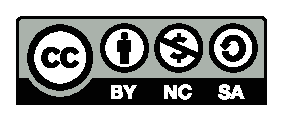
\includegraphics{CClicense.eps}}}

%\includeonly{manual/parts/part-usingtext,manual/parts/part-sections, manual/parts/part-previews,manual/parts/part-exercises}

%\includeonly{}

\begin{document}
\input table

\begin{titlepage}
\vspace*{0.5in}
\begin{center}
\fontsize{23}{12}\selectfont \textbf{Solutions for the Exercises}

\smallskip
\fontsize{23}{12}\selectfont \textbf{\emph{Mathematical Reasoning}}
%\textbf{\Huge{Mathematical Reasoning}} \\

%\smallskip
\textbf{\huge{\emph{Writing and Proof}}} \\
%\fontsize{23}{12}\selectfont \textbf{\emph{Writing and Proof}}\\
\vspace{0.3125in}
%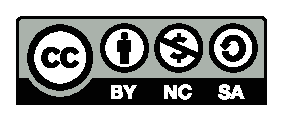
\includegraphics{CClicense.eps}
\includegraphics{CC-by-nc-sa.eps}

\vspace{0.3in}
\textbf{\large{Version 3, Version 2.1, and Version 2}} \\
\textbf{\large{\monthname~\the\day,~~\the\year}}

\vspace{1.0in}
\textbf{\huge{Ted Sundstrom}}



\smallskip
\Large{Professor Emeritus, Grand Valley State University}
\end{center}


\end{titlepage}

\newpage
\thispagestyle{empty}
$ $
\endinput



%\newpage
%\thispagestyle{empty}
%$ $

\newpage

\mainmatter
%\mainmatter
%\include{chapters/chapter1}
%\include{chapters/chapter2}
%\include{chapters/chapter3}
%\include{chapters/chapter4}
%\include{chapters/chapter5}
%\include{chapters/chapter6}
%\include{chapters/chapter7}
%\include{chapters/chapter8}
%\chapter{Finite and Infinite Sets} \label{C:topicsinsets}
\section{Finite Sets} \label{S:finitesets}
%\markboth{Chapter~\ref{C:topicsinsets}. Topics in Set Theory}{\ref{S:finitesets}. Finite Sets}
\setcounter{previewactivity}{0}
%
\begin{previewactivity}[\textbf{Equivalent Sets, Part 1}]\label{PA:equivalentsets} \hfill
\begin{enumerate}
\item Let $A$ and $B$ be sets and let $f$ be a function from $A$ to $B$.  $\left(f:A \to B \right)$.  Carefully complete each of the following using appropriate quantifiers:  (If necessary, review the material in Section~\ref{S:typesoffunctions}.)
\begin{enumerate}
\item The function $f$ is an injection provided that $\ldots .$
\item The function $f$ is not an injection provided that $\ldots .$
\item The function $f$ is a surjection provided that $\ldots .$
\item The function $f$ is not a surjection provided that $\ldots .$
\item The function $f$ is a bijection provided that $\ldots .$
\end{enumerate}
\end{enumerate}

\begin{defbox}{equivsets}{Let $A$ and $B$ be sets.  The set $A$ is \textbf{equivalent} to the set $B$ 
\index{equivalent sets}%
provided that there exists a bijection from the set $A$ onto the set $B$.  In this case, we write 
$A \approx B$.  
\label{sym:AequivB}%

\vskip6pt
When $A \approx B$, we also say that the set $A$ is in \textbf{one-to-one correspondence} 
\index{one-to-one correspondence}%
with the set $B$ and that the set $A$ has the same \textbf{cardinality} 
\index{cardinality}%
as the set $B$.
}
\end{defbox}
\noindent
\note  When $A$ is not equivalent to $B$, we write $A \not \approx B$.

%\enlargethispage{\baselineskip}
\setcounter{oldenumi}{\theenumi}
\begin{enumerate} \setcounter{enumi}{\theoldenumi}
%\begin{enumerate} \addtocounter{enumi}{1}
\item For each of the following, use the definition of equivalent sets to determine if the first set is equivalent to the second set.

\begin{enumerate}
\item $A = \left\{ 1, 2, 3 \right\}$ and $B = \left\{ a, b, c \right\}$  

\item $C = \left\{ 1, 2 \right\}$ and $B = \left\{ a, b, c \right\}$  

\item $X = \left\{ 1, 2, 3, \ldots, 10 \right\}$   and 
$Y = \left\{ 57, 58, 59, \ldots, 66 \right\}$
\end{enumerate}  

\item Let $D^+$ be the set of all odd natural numbers.   Prove that the function \linebreak
$f\x \mathbb{N} \to D^+$ defined by 
$f \left( x \right) = 2x - 1$, for all $x \in \mathbb{N}$,  is a bijection and hence that $\mathbb{N} \approx D^+$. 
\label{PA:equivalentsets5}%

%\item Let $r$ be an real number with $r > 0$.  Let $\left( 0, 1 \right)$ and 
%$\left( 0, r \right)$ be the open intervals from 0 to 1 and 0 to $r$, respectively, and let  
%$g: \left( 0, 1 \right) \to \left( 0, r \right)$ by $g \left( x \right) = rx$, for all $x \in \mathbb{R}$.  Prove that the function $g$ is a bijection and hence that 
%$\left( 0, 1 \right) \approx \left( 0, r \right)$. \label{PA:equivalentsets6}

\item Let $\R^+$ be the set of all positive real numbers.  Prove that the function 
\linebreak
$g\x \R \to \R^+$ defined by $g (x ) = e^x$, for all $x \in \R$ is a bijection and hence, that 
$\R \approx \R^+$.
\end{enumerate}
\end{previewactivity}
\hbreak

\endinput

\begin{previewactivity}[\textbf{Equivalent Sets, Part 2}]\label{PA:equivsets2} \hfill
\begin{enumerate}
\item Review Theorem~\ref{T:compositefunctions} in Section~\ref{S:compositionoffunctions}, Theorem~\ref{T:inversenotation} in Section~\ref{S:inversefunctions}, and 
Exercise~(\ref{exer:finversebijection}) in Section~\ref{S:inversefunctions}.

%\item Review the definitions of a reflexive relation on a set, a symmetric relation, a transitive relation, and an equivalence relation on a set in Section~\ref{S:equivrelations}.

\item Prove each part of the following theorem.
\begin{theorem} \label{T:equivsets} Let $A$, $B$, and $C$ be sets.

\begin{enumerate}
\item For each set $A$, $A \approx A$.  \label{T:equivsets1}

\item For all sets $A$ and $B$, if $A \approx B$, then 
$B \approx A$.  \label{T:equivsets2}

\item For all sets $A$, $B$, and $C$, if $A \approx B$ and 
$B \approx C$, then $A \approx C$.  \label{T:equivsets3}
\end{enumerate}
\end{theorem}
\end{enumerate}
%\textbf{Technical Note}:   The three properties we proved in this activity are very similar to the concepts of reflexive, symmetric, and transitive relations.  However, we do not consider equivalence of sets to be an equivalence relation on a set $U$ since an equivalence relation requires an underlying (universal) set 
%$U$.  In this case, our elements would be the sets $A$, $B$, and $C$, and these would then have to subsets of some universal set $W$ (elements of the power set of $W$).  For equivalence of sets, we are not requiring that the sets $A$, $B$, and $C$ be subsets of the same universal set.  So we do not use the term relation in regards to the equivalence of sets.  However, if $A$ and $B$ are sets and $A \equiv B$, then we often say that $A$ and $B$ are \textbf{equivalent sets}.
\end{previewactivity}
\hbreak

\endinput

%
\subsection*{Equivalent Sets}

In \typeu Activity~\ref*{PA:equivalentsets}, we introduced the concept of equivalent sets.  The motivation for this definition was to have a formal method for determining whether or not two sets ``have the same number of elements.''  This idea was described in terms of a one-to-one correspondence (a bijection) from one set onto the other set.  This idea may seem simple for finite sets, but as we will see, this idea has surprising consequences when we deal with infinite sets.  (We will soon provide precise definitions for finite and infinite sets.)

\newpar
\textbf{Technical Note}:   The three properties we proved in Theorem~\ref{T:equivsets} in \typeu Activity~\ref*{PA:equivsets2} are very similar to the concepts of reflexive, symmetric, and transitive relations.  However, we do not consider equivalence of sets to be an equivalence relation on a set $U$ since an equivalence relation requires an underlying (universal) set $U$.  In this case, our elements would be the sets $A$, $B$, and $C$, and these would then have to be subsets of some universal set $W$ (elements of the power set of $W$).  For equivalence of sets, we are not requiring that the sets $A$, $B$, and $C$ be subsets of the same universal set.  So we do not use the term relation in regards to the equivalence of sets.  However, if $A$ and $B$ are sets and 
$A \approx B$, then we often say that $A$ and $B$ are \textbf{equivalent sets}.

\hbreak

\begin{prog}[\textbf{Examples of Equivalent Sets}]\label{prog:equivsets} \hfill \\
We will use the definition of equivalent sets from \typeu Activity~\ref*{PA:equivalentsets} in all parts of this progress check.  It is no longer sufficient to say that two sets are equivalent by simply saying that the two sets have the same number of elements.

\begin{enumerate}
  \item Let $A = \left\{ 1, 2, 3, \ldots, 99, 100 \right\}$ and let 
$B = \left\{ 351, 352, 353, \ldots, 449, 450 \right\}$.  Define $f\x A \to B$ by $f(x) = x + 350$, for each $x$ in $A$.  Prove that $f$ is a bijection from the set $A$ to the set $B$ and hence, $A \approx B$.

\item Let $E$ be the set of all even integers and let $D$ be the set of all odd integers.  Prove that $E \approx D$ by proving that $F\x E \to D$, where $F \left( x \right) = x + 1$, for all $x \in E$, is a bijection.

\item Let $\left( 0, 1 \right)$ be the open interval of real numbers between 0 and 1.  Similarly, if $b \in \mathbb{R}$ with $b > 0$, let $\left( 0, b \right)$ be the open interval of real numbers between 0 and $b$. \label{A:equivsets4}

Prove that the function $f\x \left( 0, 1 \right) \to \left( 0, b \right)$ by $f \left( x \right) = bx$, for all 
$x \in \left( 0, 1 \right)$, is a bijection and hence 
$\left( 0, 1 \right) \approx \left( 0, b \right)$.
\end{enumerate}
\end{prog}
\hbreak
%
In Part~(\ref{A:equivsets4}) of Progress Check~\ref{prog:equivsets}, notice that if $b > 1$, then 
$\left( 0, 1 \right)$ is a proper subset of $\left( 0, b \right)$ and 
$\left( 0, 1 \right) \approx \left( 0, b \right)$.

Also, in Part~(\ref{PA:equivalentsets5}) of \typeu Activity~\ref*{PA:equivalentsets}, we proved that the set $D$ of all odd natural numbers is equivalent to $\mathbb{N}$, and we know that $D$ is a proper subset of $\mathbb{N}$.  

These results may seem a bit strange, but they are logical consequences of the definition of equivalent sets.  Although we have not defined the terms yet, we will see that one thing that will distinguish an infinite set from a finite set is that an infinite set can be equivalent to one of its proper subsets, whereas a finite set cannot be equivalent to one of its proper subsets.  

\endinput

\subsection*{Finite Sets}
In Section~\ref{S:setoperations}, we defined the \textbf{cardinality}
\index{cardinality!finite set}%
 of a finite set $A$, denoted by $\card (A)$, to be the number of elements in the set $A$.  Now that we know about functions and bijections, we can define this concept more formally and more rigorously.  First, for each $k \in \mathbb{N}$, we define $\mathbb{N}_k$ to be the set of all natural numbers between 1 and $k$, inclusive.  That is,
\label{sym:firstk}
\[
\mathbb{N}_k = \left\{ 1, 2, \ldots, k \right\}\!.
\]
We will use the concept of \textbf{equivalent sets}
\index{equivalent sets}%
 introduced in \typeu Activity~\ref*{PA:equivalentsets} to define a finite set.

\begin{defbox}{cardinalityfinite}{A set $A$ is a \textbf{finite set}
\index{finite set}%
\index{finite set!properties of|(}%
 provided that $A = \emptyset$ or there exists a natural number $k$ such that 
$A \approx \mathbb{N}_k$.  A set is an \textbf{infinite set}
\index{infinite set}%
 provided that it is not a finite set.

If $A \approx \mathbb{N}_k$, we say that the set $A$ has \textbf{cardinality}
\index{cardinality}%
 $\boldsymbol{k}$ (or \textbf{cardinal number}
\index{cardinal number}%
 $\boldsymbol{k}$), and we write  $\text{card} \left( A \right) = k$.  \label{sym:cardk} 

In addition, we say that the empty set has \textbf{cardinality 0} (or \textbf{cardinal number 0}), and we write $\text{card} \left( \emptyset \right) = 0$.}
\end{defbox}
%
Notice that by this definition, the empty set is a finite set.  In addition, for each 
$k \in \mathbb{N}$, the identity function on $\mathbb{N}_k$ is a bijection and hence, by definition, the set $\mathbb{N}_k$ is a finite set with cardinality $k$.

\begin{theorem}\label{T:equivfinitesets}
Any set equivalent to a finite nonempty set $A$ is a finite set and has the same cardinality as 
$A$.
\end{theorem}
%
\begin{myproof}
Suppose that $A$ is a finite nonempty set, $B$ is a set, and $A \approx B$.  Since $A$ is a finite set, there exists a $k \in \mathbb{N}$ such that $A \approx \mathbb{N}_k$.  We also have assumed that $A \approx B$ and so by part~(b) of Theorem~\ref{T:equivsets} (in \typeu Activity~\ref*{PA:equivsets2}), we can conclude that 
$B \approx A$.  Since $A \approx \mathbb{N}_k$, we can use part~(c) of Theorem~\ref{T:equivsets} to conclude that $B \approx \mathbb{N}_k$.  Thus, $B$ is finite and has the same cardinality as $A$.
\end{myproof}
%\hbreak

It may seem that we have done a lot of work to prove an ``obvious'' result in 
Theorem~\ref{T:equivfinitesets}.  The same may be true of the remaining results in this section, which give further results about finite sets.  One of the goals is to make sure that the concept of cardinality for a finite set corresponds to our intuitive notion of the number of elements in the set.  Another important goal is to lay the groundwork for a more rigorous and mathematical treatment of infinite sets than we have encountered before.  Along the way, we will see the mathematical distinction between finite and infinite sets.

The following two lemmas will be used to prove the theorem that states that every subset of a finite set is finite.

\begin{lemma} \label{L:addone}
If $A$ is a finite set and $x \notin A$, then $A \cup \left\{ x \right\}$ is a finite set and  
$\text{card} \!\left( A \cup \left\{ x \right\} \right) = \text{card}( A ) + 1$.
\end{lemma}
%
\begin{myproof}
Let $A$ be a finite set and assume $\text{card}( A ) = k$, where 
$k = 0$ or $k \in \mathbb{N}$.  Assume $x \notin A$.

If $A = \emptyset$, then $\text{card}( A ) = 0$ and 
$A \cup \left\{ x \right\} = \left\{ x \right\}$, which is equivalent to $\mathbb{N}_1$.  Thus, 
$A \cup \left\{ x \right\}$ is finite with cardinality 1, which equals 
$\text{card}( A ) + 1$.

If $A \ne \emptyset$, then $A \approx \mathbb{N}_k$, for some $k \in \mathbb{N}$.  This means that $\text{card}( A ) = k$, and there exists a bijection $f\x A \to \mathbb{N}_k$.  We will now use this bijection to define a function $g\x A \cup \left\{ x \right\} \to \mathbb{N}_{k+1}$ and then prove that the function $g$ is a bijection.  We define $g\x A \cup \left\{ x \right\} \to \mathbb{N}_{k+1}$ as follows:  For each 
$t \in A \cup \left\{ x \right\}$,
\[
g \left( t \right) = \left\{ \begin{gathered}
  f \left( t \right) \text{  if  }t \in A \hfill \\
  k + 1 \text{  if  }t = x. \hfill \\ 
\end{gathered}  \right.
\]
To prove that $g$ is an injection, we let $x_1, x_2 \in A \cup \left\{ x \right\}$ and assume 
$x_1 \ne x_2$.
\begin{itemize}
\item If $x_1, x_2 \in A$, then since $f$ is a bijection, 
$f( x_1 ) \ne f ( x_2 )$, and this implies that 
$g( x_1 ) \ne g( x_2 )$.

\item If $x_1 = x$, then since $x_2 \ne x_1$, we conclude that $x_2 \ne x$ and hence 
$x_2 \in A$.  So $g( x_1 ) = k + 1$, and since $f( x_2 ) \in \mathbb{N}_k$ and 
$g( x_2 ) = f ( x_2 )$, we can conclude that $g( x_1 ) \ne g( x_2 )$.

\item The case where $x_2 = x$ is handled similarly to the previous case.
\end{itemize}

\noindent
This proves that the function $g$ is an injection.  The proof that $g$ is a surjection is 
Exercise~(\ref{exer:addonesurjection}).  Since $g$ is a bijection, we conclude that $A \cup \left\{ x \right\} \approx \mathbb{N}_{k+1}$, and
\[
\text{card} \!\left(A \cup \left\{ x \right\} \right) = k + 1.
\]
Since $\text{card} \left(A \right) = k$, we have proved that
$\text{card} \!\left(A \cup \left\{ x \right\} \right) = \text{card}( A ) + 1.$
\end{myproof}
%\hbreak
%
%Lemma~\ref{L:addone} implies that adding one element to a finite set increases its cardinality by %one.  It is also true that removing one element from a finite set reduces the cardinality by one.  %The proof of Corollary~\ref{C:removeone} is left as Exercise~(\ref{exer:sec92corollary}).

%\begin{corollary} \label{C:removeone}
%If $A$ is a finite set and $x \in A$, then $A - \left\{ x \right\}$ is a finite set and  
%$\text{card} \left( A - \left\{ x \right\} \right) = \text{card} \left( A \right) - 1$.
%\end{corollary}
%\hbreak
%
\begin{lemma} \label{L:subsetsofNk}
For each natural number $m$, if $A \subseteq \mathbb{N}_m$, then $A$ is a finite set and 
$\text{card} \left( A \right) \leq m$.
\end{lemma}
%
\begin{myproof}
We will use a proof using induction on $m$.  For each $m \in \mathbb{N}$, let 
$P( m )$ be, ``If $A \subseteq \mathbb{N}_m$, then $A$ is finite and 
$\text{card}( A ) \leq m$.''

We first prove that $P( 1 )$ is true.  If $A \subseteq \mathbb{N}_1$, then 
$A = \emptyset$ or $A = \left\{ 1 \right\}$, both of which are finite and have cardinality less than or equal to the cardinality of $\mathbb{N}_1$.  This proves that $P( 1 )$ is true.

%\vskip6pt
For the inductive step, let $k \in \mathbb{N}$ and assume that $P( k )$ is true.  That is, assume that if $B \subseteq \mathbb{N}_k$, then $B$ is a finite set and 
$\text{card}( B ) \leq k$.  We need to prove that 
$P( k+1 )$ is true.

So assume that $A$ is a subset of $\mathbb{N}_{k+1}$.  Then $A - \left\{ k+1 \right\}$ is a subset of $\mathbb{N}_k$.  Since $P( k )$ is true, $A - \left\{ k+1 \right\}$ is a finite set and 
\[
\text{card} \!\left( A - \left\{ k+1 \right\} \right) \leq k.
\]
There are two cases to consider:  Either $k+1 \in A$ or $k+1 \not \in A$.

\vskip6pt
If $k+1 \not \in A$, then $A = A - \left\{ k+1 \right\}$.  Hence, $A$ is finite and
\[
\text{card} ( A ) \leq k < k+1.
\]

If $k+1 \in A$, then $A = ( A - \left\{ k+1 \right\} ) \cup \left\{ k+1 \right\}$. Hence, by Lemma~\ref{L:addone}, $A$ is a finite set and
\[
\text{card} ( A ) = 
\text{card} \!\left(  A - \left\{ k+1 \right\}  \right) + 1.
\]
Since $\text{card} \!\left( A - \left\{ k+1 \right\} \right) \leq k$, we can conclude that 
$\text{card} ( A ) \leq k + 1$. 

This means that we have proved the inductive step.  Hence, by mathematical induction, for each 
$m \in \mathbb{N}$, if $A \subseteq \mathbb{N}_m$, then $A$ is finite and 
$\text{card} ( A ) \leq m$.
\end{myproof}
%\hbreak
The preceding two lemmas were proved to aid in the proof of the following theorem.

\begin{theorem} \label{T:finitesubsets}
If $S$ is a finite set and $A$ is a subset of $S$, then $A$ is a finite set and 
$\text{card} ( A ) \leq \text{card} ( S )$.
\end{theorem}
%
\begin{myproof}
Let $S$ be a finite set and assume that $A$ is a subset of $S$.  If $A = \emptyset$, then $A$ is a finite set and $\text{card} ( A ) \leq \text{card} ( S )$.  So we assume that $A \ne \emptyset$.  

Since $S$ is finite, there exists a bijection $f\x S \to \mathbb{N}_k$ for some $k \in \mathbb{N}$.  In this case, $\text{card} ( S ) = k$.  We need to show that $A$ is equivalent to a finite set.  To do this, we define 
$g\x A \to f ( A )$ by
\begin{center}
$g ( x ) = f ( x )$ for each $x \in A$.
\end{center}
Since $f$ is an injection, we conclude that $g$ is an injection.  Now let 
$y \in f ( A )$.  Then there exists an $a \in A$ such that $f ( a ) = y$.  But by the definition of $g$, this means that $g ( a ) = y$, and hence $g$ is a surjection.  This proves that $g$ is a bijection.

Hence, we have proved that $A \approx f ( A )$.  Since $f ( A )$ is a subset of $\mathbb{N}_k$, we use Lemma~\ref{L:subsetsofNk} to conclude that $f ( A )$ is finite and $\text{card} ( f ( A ) ) \leq k$.  In addition, by 
Theorem~\ref{T:equivfinitesets}, $A$ is a finite set and 
$\text{card} ( A ) = \text{card} ( f ( A ) )$.  This proves that $A$ is a finite set and $\text{card} ( A ) \leq \text{card} ( S )$.
\end{myproof}
\hbreak

Lemma~\ref{L:addone} implies that adding one element to a finite set increases its cardinality by 1.  It is also true that removing one element from a finite nonempty set reduces the cardinality by 1.  The proof of Corollary~\ref{C:removeone} is 
Exercise~(\ref{exer:sec92corollary}).

\begin{corollary} \label{C:removeone}
If $A$ is a finite set and $x \in A$, then $A - \left\{ x \right\}$ is a finite set and  
$\text{card} \!\left( A - \left\{ x \right\} \right) = \text{card} ( A ) - 1$.
\end{corollary}
%
The next corollary will be used in the next section to provide a mathematical distinction between finite and infinite sets.
\begin{corollary} \label{C:propersubsets}
A finite set is not equivalent to any of its proper subsets.
\end{corollary}
%
\begin{myproof}
Let $B$ be a finite set and assume that $A$ is a proper subset of $B$.  Since $A$ is a proper subset of $B$, there exists an element $x$ in $B - A$.  This means that $A$ is a subset of 
$B - \left\{ x \right\}$.  Hence, by Theorem~\ref{T:finitesubsets},
\[
\text{card} ( A ) \leq \text{card} \!\left( B - \left\{ x \right\} \right).
\]
Also, by Corollary~\ref{C:removeone}
\[
\text{card} \!\left( B - \left\{ x \right\} \right) = \text{card} ( B ) - 1.
\]
Hence, we may conclude that $\text{card} ( A ) \leq \text{card} ( B ) - 1$ and that 
\[
\text{card} ( A ) < \text{card} ( B ).
\]
Theorem~\ref{T:equivfinitesets}
implies that $B \not \approx A$.  This proves that a finite set is not equivalent to any of its proper subsets.
\end{myproof}
\hbreak

\endinput

\subsection*{The Pigeonhole Principle}

The last property of finite sets that we will consider in this section is often called the 
\textbf{Pigeonhole Principle}.
\index{Pigeonhole Principle}%
  The ``pigeonhole'' version of this property says,  ``If $m$ pigeons go into $r$ pigeonholes and $m > r$, then at least one pigeonhole has more than one pigeon.''

In this situation, we can think of the set of pigeons as being equivalent to a set $P$ with cardinality $m$ and the set of pigeonholes as being equivalent to a set $H$ with cardinality 
$r$.  We can then define a function $f\x P \to H$ that maps each pigeon to its pigeonhole.  The Pigeonhole Principle states that this function is not an injection.  (It is not one-to-one since there are at least two pigeons ``mapped'' to the same pigeonhole.)

\begin{theorem} [\textbf{The Pigeonhole Principle}] \label{T:pigeonhole}
Let $A$ and $B$ be finite sets.  If $\text{card} ( A ) > \text{card} ( B )$, then any function $f\x A \to B$ is not an injection.
\end{theorem}
%
\begin{myproof}
Let $A$ and $B$ be finite sets. We will prove the contrapositive of the theorem, which is, 
if there exists a function $f\x A \to B$ that is an injection, then 
$\text{card} ( A ) \leq \text{card} ( B )$.

So assume that $f\x A \to B$ is an injection.  As in Theorem~\ref{T:finitesubsets}, we define a function $g\x A \to f ( A )$ by 
\begin{center}
$g ( x ) = f ( x )$ for each $x \in A$.
\end{center}
As we saw in Theorem~\ref{T:finitesubsets}, the function $g$ is a bijection.  But then 
$A \approx f ( A )$ and $f ( A ) \subseteq B$.  Hence, 
\begin{center}
$\text{card} ( A ) = \text{card} \!\left( f ( A ) \right)$ and 
$\text{card} \!\left( f ( A ) \right) \leq \text{card} ( B )$.
\end{center}
Hence, $\text{card} ( A ) \leq \text{card} ( B )$, and this proves the contrapositive.  Hence, if $\text{card} ( A ) > \text{card} ( B )$, then  any function $f\x A \to B$  is not an injection.
\end{myproof}
The Pigeonhole Principle has many applications in the branch of mathematics called ``combinatorics.''  Some of these will be explored in the exercises.
\hbreak
\index{finite set!properties of|)}%

\endinput


\endinput




\hbreak

\endinput

\begin{example}
Let $\mathcal{F}$ be the set of all functions from $\mathbb{N}$ to the set 
$\left\{ 0, 1 \right\}$.  This set is often denoted by $\left\{ 0, 1 \right\}^\mathbb{N}$.  We will prove that $\mathcal{F} \approx \mathcal{P} ( \mathbb{N} )$, the power set of 
$\mathbb{N}$.

To prove that $\mathcal{F} \approx \mathcal{P} ( \mathbb{N} )$, we will construct a function $G\x \mathcal{F} \to \mathcal{P} ( \mathbb{N} )$ and then prove that $G$ is a bijection.  Notice that the domain of the function $G$ will be a set of functions.  So, the inputs for $G$ will themselves be functions with domain $\mathbb{N}$ and codomain 
$\left\{ 0, 1 \right\}$.

So, we define $G\x \mathcal{F} \to \mathcal{P} ( \mathbb{N} )$ as follows:
\[
\text{For } f \in \mathcal{F}, \quad G ( f ) = \left\{x \in \mathbb{N} \mid 
f ( x ) = 1 \right\}.
\]
Notice that $G ( f ) \subseteq \mathbb{N}$ and hence 
$G ( f ) \in \mathcal{P} ( \mathbb{N} )$.

To prove that the function $G$ is an injection, we let $f_1, f_2 \in \mathcal{F}$ and suppose that 
$f_1 \ne f_2$.  Since $f_1\x  \mathbb{N} \to \left\{ 0, 1 \right\}$ and 
$f_2\x  \mathbb{N} \to \left\{ 0, 1 \right\}$, this means that 
\begin{center}
there exists an $m \in \mathbb{N}$ such that $f_1 ( m ) \ne f_2 ( m )$.
\end{center}
Since the codomain of both $f_1$ and $f_2$ is $\left\{ 0, 1 \right\}$, we may assume that 
$f_1 ( m ) = 1$ and $f_2 ( m ) = 0$.  (The proof for the case where 
$f_1 ( m ) = 0$ and $f_2 ( m ) = 1$ is similar.)  But then
\[
m \in \left\{x \in \mathbb{N} \mid f_1 ( x ) = 1 \right\} \text{ and } 
m \not \in \left\{x \in \mathbb{N} \mid f_2 ( x ) = 1 \right\}.
\]
That is, $m \in G ( f_1 )$ and $m \not \in G ( f_2 )$.  Hence, 
$G ( f_1 ) \ne G ( f_2 )$.  This proves that $G$ is an injection.

To show that $G$ is a surjection, we let $B \in \mathcal{P} ( \mathbb{N} )$.  So, 
$B \subseteq \mathbb{N}$.  We need to find a function $f \in \mathcal{F}$ such that 
$G ( f ) = B$.  We will use the \textbf{characteristic function} of the set $B$.  This was introduced in Section~\ref{S:moreaboutfunctions} on page~\pageref{charfunction}, and is defined as follows:  $\chi _B \x \mathbb{N} \to \left\{ {0, 1} \right\}$ by
\[
\chi _B ( x ) = \left\{ \begin{gathered}
  1\text{  if  }x \in B \hfill \\
  0\text{  if  }x \notin B \hfill \\ 
\end{gathered}  \right.
\]
Therefore, 
\[
G ( \chi_B ) = \left\{x \in \mathbb{N} \mid \chi_B ( x ) = 1 \right\} = B.
\]
This proves that the function $G$ is a surjection, and hence, $G$ is a bijection.  Therefore, we have proved that $\mathcal{F} \approx \mathcal{P} ( \mathbb{N} )$.
\end{example}
\hbreak
%


Hence,
$\text{card} ( A ) = k$.

Also, $\left\{ x \right\} \approx \left\{ k + 1 \right\}$.  In addition, 
$A \cap \left\{ x \right\} = \emptyset$ and 
$\mathbb{N}_k \cap \left\{ k + 1 \right\} = \emptyset$.  Hence, by Theorem~\ref{T:equivalentsets},
\[
A \cup \left\{ x \right\} \approx \mathbb{N}_k \cup \left\{ k + 1 \right\} = \mathbb{N}_{k+1}.
\]
This proves that $A \cup \left\{ x \right\}$ is a finite set with cardinality $k + 1$, and hence 
$\text{card} ( A \cup \left\{ x \right\} ) = \text{card} ( A ) + 1$.



We will now state a theorem that will prove useful in our study of equivalent sets.  Its proof will be outlined in Activity~\ref{A:theoremequivsets}

\begin{theorem} \label{T:equivalentsets}
Let $A$, $B$, $C$, and $D$ be sets with $A \approx B$ and $C \approx D$.  Then:
\begin{enumerate}
\item $A \times C \approx B \times D$. \label{T:equivalentsets1}

\item If $A$ and $C$ are disjoint and $B$ and $D$ are disjoint, then 
$A \cup C \approx B \cup D$. \label{T:equivalentsets2}
\end{enumerate}
\end{theorem}

\begin{activity}[Proof of Theorem~\ref{T:equivalentsets}] \label{A:theoremequivsets}

Let $A$, $B$, $C$, and $D$ be sets with $A \approx B$ and $C \approx D$.  Since $A \approx B$ and 
$C \approx D$, there exist bijections $f\x A \to B$ and $g\x C \to D$.

\begin{enumerate}
\item To prove that $A \times C \approx B \times D$, prove that the following function is a bijection:  $h\x A \times C \to B \times D$ where
\[
h ( a, c ) = ( f ( a ), g ( c ) )
\]
for all $( a, c ) \in A \times C$.

\item Now assume that $A \cap C = \emptyset$ and $B \cap D = \emptyset$.  To prove that 
$A \cup C \approx B \cup D$, prove that the following function is a bijection:  
$k\x A \cup C \to B \cup D$ where
\[
k ( x ) = \left\{ \begin{gathered}
  f ( x ) \text{  if  }x \in A \hfill \\
  g ( x ) \text{  if  }x \notin B \hfill \\ 
\end{gathered}  \right.
\]
for all $( a, c ) \in A \times C$.
\end{enumerate}
\end{activity}
\hbreak


\section*{Exercises \ref{S:finitesets}}

\begin{enumerate}
\item Prove that the function $g: A \cup \left\{ x \right\} \to \N_{k+1}$ in 
Lemma~\ref{L:addone} is a surjection. 
\label{exer:addonesurjection}%

\xitem Let $A$ be a subset of some universal set $U$.  Prove that if $x \in U$\!, then 
\linebreak $A \times \left\{ x \right\} \approx A$. 
\label{exer:sec92-1}%

\xitem Let $E^+$ be the set of all even natural numbers.  Prove that $\mathbb{N} \approx E^+$. \label{exer91:evennaturals}

\xitem  Prove Corollary~\ref{C:removeone}. 
\label{exer:sec92corollary}%

If $A$ is a finite set and $x \in A$, then $A - \left\{ x \right\}$ is a finite set and  \\
$\text{card} ( A - \left\{ x \right\} ) = \text{card} ( A ) - 1$.

\hint  One approach is to use the fact that $A = \left( A - \left\{ x \right\} \right) \cup \left\{x \right\}$.

\item Let $A$ and $B$ be sets.  Prove that 
\label{exer:sec92-finitesets}%
\begin{enumerate}
\yitem If $A$ is a finite set, then $A \cap B$ is a finite set.

\yitem If $A \cup B$ is a finite set, then $A$ and $B$ are finite sets.

\item If $A \cap B$ is an infinite set, then $A$ is an infinite set.

\item If $A$ is an infinite set or $B$ is an infinite set, then $A \cup B$ is an infinite set.
\end{enumerate}

\item There are over 7 million people living in New York City.  It is also known that the maximum number of hairs on a human head is less than 200,000.  Use the Pigeonhole Principle to prove that there are at least two people in the city of New York with the same number of hairs on their heads. 
\label{exer:sec92-pigeon}%


\item Prove the following propositions: 
\label{exer:sec92-7}%
\begin{enumerate}
\yitem If $A$, $B$, $C$, and $D$ are sets with $A \approx B$ and $C \approx D$,  then \linebreak
$A \times C \approx B \times D$. 
\label{exer:equivcartesian}%

\item If $A$, $B$, $C$, and $D$ are sets with $A \approx B$ and $C \approx D$ and if $A$ and $C$ are disjoint and $B$ and $D$ are disjoint, then $A \cup C \approx B \cup D$. 
\label{exer:equivunion}%
\end{enumerate}

\hint Since $A \approx B$ and $C \approx D$, there exist bijections $f:A \to B$ and $g:C \to D$.  To prove that $A \times C \approx B \times D$, prove that 
$h:A \times C \to B \times D$ is a bijection, where 
$h ( a, c ) = \left( f ( a ), g ( c ) \right)$, 
for all $( a, c ) \in A \times C$.

%If $A \cap C = \emptyset$ and $B \cap D = \emptyset$, then to prove that 
%$A \cup C \approx B \cup D$, prove that the following function is a bijection:  
%$k:A \cup C \to B \cup D$, where
%\[
%k ( x ) = \left\{ \begin{gathered}
%  f ( x ) \text{  if  }x \in A \hfill \\
%  g ( x ) \text{  if  }x \in C. \hfill \\ 
%\end{gathered}  \right.
%\]

\item Let  $A = \left\{ a, b, c \right\}$. 
\label{exer:sec927}%
\begin{enumerate}
\yitem Construct a function $f:\mathbb{N}_5 \to A$ such that $f$ is a surjection.

\item Use the function $f$ to construct a function $g:A \to \mathbb{N}_5$ so that \linebreak
$f \circ g = I_A$, where $I_A$ is the identity function on the set $A$.  Is the function $g$ an injection?  Explain.
\end{enumerate}

\item This exercise is a generalization of Exercise~(\ref{exer:sec927}). Let $m$ be a natural number, let $A$ be a set, and assume that $f:\mathbb{N}_m \to A$ is a surjection.  Define \linebreak
$g:A \to \mathbb{N}_m$ as follows: 
\label{exer:sec928}%

\begin{list}{}
\item For each $x \in A$, $g ( x ) = j$, where $j$ is the least natural number in 
$f^{-1} ( \left\{ x \right\} ) $.
\end{list}

Prove that $f \circ g = I_A$, where $I_A$ is the identity function on the set $A$, and prove that $g$ is an injection.

\item Let $B$ be a finite, nonempty set and assume that $f:B \to A$ is a surjection.  Prove that there exists a function $h:A \to B$ such that $f \circ h = I_A$ and $h$ is an injection.

\hint  Since $B$ is finite, there exists a natural number $m$ such that $\mathbb{N}_m \approx B$.  This means there exists a bijection $k:\mathbb{N}_m \to B$.  Now let $h = k \circ g$, where $g$ is the function constructed in Exercise~(\ref{exer:sec928}).

\end{enumerate}



\subsection*{Explorations and Activities}
\setcounter{oldenumi}{\theenumi}
\begin{enumerate} \setcounter{enumi}{\theoldenumi}
\item \textbf{Using the Pigeonhole Principle}.  \label{A:usingpigeon} 
\index{Pigeonhole Principle}%
For this activity, we will consider subsets of $\mathbb{N}_{30}$ that contain eight elements.  

\begin{enumerate}
\item One such set is $A = \left\{ 3, 5, 11, 17, 21, 24, 26, 29 \right\}$.  Notice that
\begin{align}
\left\{3, 21, 24, 26 \right\} &\subseteq A \quad \text{ and }   &3 + 21 + 24 + 26 &= 74 \notag \\
\left\{3, 5, 11, 26, 29 \right\} &\subseteq A \quad \text{ and }   &3 + 5 + 11 + 26 + 29 &= 74. \notag
\end{align}
Use this information to find two disjoint subsets of $A$ whose elements have the same sum.
\label{A:usingpigeon1}

\item Let $B = \left\{ 3, 6, 9, 12, 15, 18, 21, 24 \right\}$.  Find two disjoint subsets of $B$ whose elements have the same sum.  \note  By convention, if $T = \left\{ a \right\}$, where $a \in \mathbb{N}$, then the sum of the elements in $T$ is equal to $a$.

\item Now let $C$ be any subset of $\mathbb{N}_{30}$ that contains eight elements.
\begin{enumerate}
\item How many subsets does $C$ have?
\item The sum of the elements of the empty set is 0.  What is the maximum sum for any subset of 
$\mathbb{N}_{30}$ that contains eight elements?  Let $M$ be this maximum sum.

%\hint  Make the elements of a subset of $\mathbb{N}_{30}$ with 8 elements as large as possible.

\item Now define a function $f\x \mathcal{P} ( C ) \to \mathbb{N}_M$ so that for each 
$X \in \mathcal{P} ( C )$, $f ( X )$ is equal to the sum of the elements in $X$.

Use the Pigeonhole Principle to prove that there exist two subsets of $C$ whose elements have the same sum. \label{A:usingpigeon3c}
\end{enumerate}

\item If the two subsets in part~(\ref{A:usingpigeon3c}) are not disjoint, use the idea presented in part~(\ref{A:usingpigeon1}) to prove that there exist two disjoint subsets of $C$ whose elements have the same sum.


\item Let $S$ be a subset of $\mathbb{N}_{99}$ that contains 10 elements.  Use the Pigeonhole Principle to prove that there exist two disjoint subsets of $S$ whose elements have the same sum.
\label{exer:sec92-pigeon2}%
\end{enumerate}

\end{enumerate}


\hbreak

\endinput


\section{Countable Sets}\label{S:infinitesets}
%\markboth{Chapter~\ref{C:topicsinsets}. Topics in Set Theory}{\ref{S:infinitesets}. Countable 
%Sets}
\setcounter{previewactivity}{0}
%
\begin{previewactivity}[\textbf{Introduction to Infinite Sets}]\label{PA:introtoinfinite} \hfill \\
In Section~\ref{S:finitesets}, we defined a \textbf{finite set}
\index{finite set}%
 to be the empty set or a set $A$ such that $A \approx \mathbb{N}_k$ for some natural number $k$.    We also defined an 
\textbf{infinite set} 
\index{infinite set}%
to be a set that is not finite, but the question now is, ``How do we know if a set is infinite?''  
One way to determine if a set is an infinite set is to use 
Corollary~\ref{C:propersubsets}, which states that a finite set is not equivalent to any of its subsets.  We can write this as a conditional statement as follows:

\begin{list}{}
\item If $A$ is a finite set, then $A$ is not equivalent to any of its proper subsets.
\end{list}
\noindent
or more formally as
\begin{list}{}
\item For each set $A$, if $A$ is a finite set, then for each proper subset $B$ of $A$, $A \not\approx B$.
\end{list}

\begin{enumerate}
\item Write the contrapositive of the preceding conditional statement.  Then explain how this statement can be used to determine if a set is infinite.

\item Let $D^+$ be the set of all odd natural numbers.  In \typeu Activity~\ref*{PA:equivalentsets} from Section~\ref{S:finitesets}, we proved that $\mathbb{N} \approx D^+$. 
\label{PA:introtoinfinite2}%

\begin{enumerate}
\item Use this to explain carefully why $\mathbb{N}$ is an infinite set.

\item Is $D^+$ a finite set or an infinite set?  Explain carefully  how you know.
\end{enumerate}

\item Let $b$ be a positive real number.  Let $( 0, 1 )$ and 
$( 0, b )$ be the open intervals from 0 to 1 and 0 to $b$, respectively.  In 
Part~(\ref{A:equivsets4}) of Progress Check~\ref{prog:equivsets} 
(on page~\pageref{prog:equivsets}), 
%Beginning Activity~\ref{PA:equivalentsets} from Section~\ref{S:finitesets}, 
we proved that 
$( 0, 1 ) \approx ( 0, b )$. 
\label{PA:introtoinfinite3}%

\begin{enumerate}
\item Use a value for $b$ where $0 < b < 1$ to explain why $( 0, 1 )$ is an infinite set.

\item Use a value for $b$ where $b > 1$ to explain why $( 0, b )$ is an infinite set.
\end{enumerate}

\end{enumerate}
\end{previewactivity}
%\hbreak

\endinput




\begin{previewactivity}[\textbf{A Function from $\boldsymbol{\N}$ to $\boldsymbol{\Z}$}]\label{PA:functionNtoZ} \hfill \\
In this activity, we will define and explore a function $f:\mathbb{N} \to \mathbb{Z}$.  We will start by defining $f ( n )$ for the first few natural numbers $n$.

\begin{center}
\begin{tabular}[h]{l p{2cm} l}
$f ( 1 ) = 0$  &  &  \\
$f ( 2 ) = 1$  &  &  $f ( 3 ) = -1$ \\
$f ( 4 ) = 2$  &  &  $f ( 5 ) = -2$ \\
$f ( 6 ) = 3$  &  &  $f ( 7 ) = -3$\\
\end{tabular}
\end{center}
Notice that if we list the outputs of $f$ in the order 
$f ( 1 ), f ( 2 ), f ( 3 ), \ldots$,  we create the following list of integers:
$0, 1, -1, 2, -2, 3, -3, \ldots$.  We can also illustrate the outputs of this function with the following diagram:
\begin{figure}[h]
$$
\BeginTable
\BeginFormat
| c | c | c | c | c | c | c | c | c | c | c |
\EndFormat
" 1 " 2 " 3 " 4 " 5 " 6 " 7 " 8 " 9 " 10 " $\cdots$ " \\
" $\downarrow$ " $\downarrow$ " $\downarrow$ " $\downarrow$ " $\downarrow$ " $\downarrow$ " $\downarrow$ " $\downarrow$ " $\downarrow$ " $\downarrow$ " $\cdots$ "\\
" 0 " 1 " $-1$ " 2 " $-2$ " 3 " $-3$ " 4 " $-4$ " 5 "  $\cdots$ " \\
\EndTable
$$
\caption{A Function from $\N$ to $\Z$} \label{fig:functionNtoZ}
\end{figure}


\begin{enumerate}
\item If the pattern suggested by the function values we have defined continues, what are 
$f ( 11 )$ and $f ( 12 )$?  What is $f ( n )$ for $n$ from 13 to 16? 
\label{PA:functionNtoZ1}%

\item If the pattern of outputs continues, does the function $f$ appear to be an injection?  Does $f$ appear to be a surjection?  (Formal proofs are not required.)
\end{enumerate}

We will now attempt to determine a formula for $f ( n )$, where $n \in \mathbb{N}$.  We will actually determine two formulas:  one for when $n$ is even and one for when $n$ is odd.

\begin{enumerate} \setcounter{enumi}{2}
\item Look at the pattern of the values of $f ( n )$ when $n$ is even.  What appears to be a formula for $f ( n )$ when $n$ is even? 
\label{PA:functionNtoZ3}%

\item Look at the pattern of the values of $f ( n )$ when $n$ is odd.  What appears to be a formula for $f ( n )$ when $n$ is odd? 
\label{PA:functionNtoZ4}%

\item Use the work in Part~(\ref{PA:functionNtoZ3}) and Part~(\ref{PA:functionNtoZ4}) to complete the following:  Define $f\x \mathbb{N} \to \mathbb{Z}$, where
\[
f ( n ) = \left\{ \begin{gathered}
  ?? \text{  if  }n \text{ is even} \hfill \\
\\
  ?? \text{  if  }n \text{ is odd}. \hfill \\ 
\end{gathered}  \right.
\]
\label{PA:functionNtoZ5}%

\item Use the formula in Part~(\ref{PA:functionNtoZ5}) to
\begin{enumerate}
\item Calculate $f ( 1 )$ through $f ( 10 )$.  Are these results consistent with the pattern exhibited at the start of this activity?

\item Calculate $f ( 1000 )$ and $f ( 1001 )$.

\item Determine the value of $n$ so that $f ( n ) = 1000$.
\end{enumerate}
\end{enumerate} 
\end{previewactivity}
\hbreak

\endinput

%
In this section, we will describe several infinite sets and define the cardinal number for so-called countable sets.  Most of our examples will be subsets of some of our standard number systems such as $\mathbb{N}$, $\mathbb{Z}$, and $\mathbb{Q}$.  

%We will see that there are infinite sets that may appear to be different in size, and that there exist infinite sets that are not equivalent.

\subsection*{Infinite Sets}
In \typeu Activity~\ref*{PA:introtoinfinite}, we saw how to use Corollary~\ref{C:propersubsets} to prove that a set is infinite.  This corollary implies that if $A$ is a finite set, then $A$ is not equivalent to any of its proper subsets.  By writing the contrapositive of this conditional statement, we can restate Corollary~\ref{C:propersubsets} in the following form:

\vskip9pt
\noindent
\textbf{Corollary~\ref{C:propersubsets}}.
\emph{If a set $A$ is equivalent to one of its proper subsets, then $A$ is infinite.}

%\begin{theorem} \label{T:infinitesets}
%The set $A$ is an infinite set if and only if $A$ is equivalent to one of its proper subsets.
%\end{theorem}

%\begin{example} 
\newpar
In \typeu Activity~\ref*{PA:introtoinfinite}, we used Corollary~\ref{C:propersubsets} to prove that
\begin{itemize}
\item The set of natural numbers, $\mathbb{N}$, is an infinite set.

\item The open interval $( 0, 1 )$ is an infinite set.
\end{itemize}
%\end{example}
Although Corollary~\ref{C:propersubsets} provides one way to prove that a set is infinite, it is sometimes more convenient to use a proof by contradiction to prove that a set is infinite.  The idea is to use results from Section~\ref{S:finitesets} about finite sets to help obtain a contradiction.  This is illustrated in the next theorem.
\begin{theorem}\label{T:subsetisinfinite}
Let $A$ and $B$ be sets.
\begin{enumerate}
\item If $A$ is infinite and $A \approx B$, then $B$ is infinite.  \label{T:subsetisinfinite1}
\item If $A$ is infinite and $A \subseteq B$, then $B$ is infinite.  \label{T:subsetisinfinite2}
\end{enumerate}
\end{theorem}
%
\begin{myproof}
We will prove part~(\ref{T:subsetisinfinite1}).  The proof of part~(\ref{T:subsetisinfinite2}) is exercise~(\ref{exer:subsetisinfinite}) on page~\pageref{exer:subsetisinfinite}.

To prove part~(\ref{T:subsetisinfinite1}), we use a proof by contradiction and assume that $A$ is an infinite set, $A \approx B$, and $B$ is not infinite.  That is, $B$ is a finite set.  Since $A \approx B$ and $B$ is finite, Theorem~\ref{T:equivfinitesets} on page~\pageref{T:equivfinitesets} implies that $A$ is a finite set.  This is a contradiction to the assumption that $A$ is infinite.  We have therefore proved that if $A$ is infinite and $A \approx B$, then $B$ is infinite.
\end{myproof}

%\begin{activity}[Proof of Theorem~\ref{T:subsetisinfinite}] \label{A:subsetisfinite}
%Write a proof for both parts of Theorem~\ref{T:subsetisinfinite}.  For both parts, use a proof by contradiction.  For each proof, a theorem in Section~\ref{S:finitesets} will provide a contradiction.
%\end{activity}
\hbreak
%
%\begin{example}[Examples of Infinite Sets] \label{E:infinitesets} \hfill
%\begin{itemize}
%\item Theorem~\ref{T:subsetisinfinite} allows us to conclude that our standard number systems are infinite sets since they all have $\mathbb{N}$ as a subset.  So $\mathbb{Z}$, $\mathbb{Q}$, and $\mathbb{R}$ are all infinite sets.  In addition, the set of all positive rational numbers, 
%$\mathbb{Q}^+$, and the set of all positive real numbers, $\mathbb{R}^+$, are infinite sets.
%
%\item Let $D^+$ be the set of all odd natural numbers.  In Part~(\ref{PA:introtoinfinite2}) of Beginning Activity~\ref{PA:introtoinfinite}, we proved that $D^+ \approx \mathbb{N}$.  Therefore, by Theorem~\ref{T:subsetisinfinite}, $D^+$ is an infinite set.  In a similar manner, the set $E^+$ of all even natural numbers is an infinite set.  To do this, we can use the function $g\x \mathbb{N} \to E^+$ defined by $g ( x ) = 2x$ for all $x \in \mathbb{N}$.
%\end{itemize}
%\end{example}
\begin{prog}[\textbf{Examples of Infinite Sets}] \label{E:infinitesets} \hfill
\begin{enumerate}
\item In \typeu Activity~\ref*{PA:introtoinfinite}, we used Corollary~\ref{C:propersubsets} to prove that $\N$ is an infinite set.  Now use this and Theorem~\ref{T:subsetisinfinite} to explain why our standard number systems $( \Z, \Q, \text{ and } \R )$ are infinite sets.  Also, explain why the set of all positive rational numbers, 
$\Q^+$, and the set of all positive real numbers, $\R^+$, are infinite sets.

\item Let $D^+$ be the set of all odd natural numbers.  In Part~(\ref{PA:introtoinfinite2}) of \typeu Activity~\ref*{PA:introtoinfinite}, we proved that $D^+ \approx \mathbb{N}$.  Use 
Theorem~\ref{T:subsetisinfinite} to explain why $D^+$ is an infinite set.  

\item Prove that the set $E^+$ of all even natural numbers is an infinite set.
\end{enumerate}
\end{prog}
\hbreak

\endinput


\subsection*{Countably Infinite Sets}
In Section~\ref{S:finitesets}, we used the set $\mathbb{N}_k$ as the standard set with cardinality $k$ in the sense that a set is finite if and only if it is equivalent to 
$\mathbb{N}_k$.  In a similar manner, we will use some infinite sets as standard sets for certain infinite cardinal numbers.  The first set we will use is $\mathbb{N}$.  

We will formally define what it means to say the elements of a set can be ``counted'' using the natural numbers.  The elements of a finite set can be ``counted'' by defining a bijection (one-to-one correspondence) between the set and $\mathbb{N}_k$ for some natural number $k$.  We will be able to ``count'' the elements of an infinite set if we can define a one-to-one correspondence between the set and $\mathbb{N}$.

\begin{defbox}{aleph0}{The \textbf{cardinality of} $\boldsymbol{\mathbb{N}}$
\index{cardinality}%
\index{cardinality!natural numbers}%
\index{cardinality!$\aleph_0$}%
%\index{$\aleph_0$}%
 is denoted by $\aleph_0$.  
\label{sym:aleph0}%
 The symbol $\aleph$ is the first letter of the Hebrew alphabet, \textbf{aleph}.
\index{aleph}%
  The subscript 0 is often read as ``naught'' (or sometimes as ``zero'' or ``null'').  So we write
\[
\text{card}( \N ) = \aleph_0
\]
and say that the cardinality of $\mathbb{N}$ is ``aleph naught.''}
\end{defbox}
%
\begin{defbox}{countinfinite}{A set $A$ is \textbf{countably infinite}
\index{countably infinite set}%
 provided that 
$A \approx \mathbb{N}$.  In this case, we write
\[
\text{card}( A ) = \aleph_0.
\]
A set that is countably infinite is sometimes called a \textbf{denumerable}
\index{denumerable set}%
 set.  A set is 
\textbf{countable}
\index{countable set}%
 provided that it is finite or countably infinite.  An infinite set that is not countably infinite is called an \textbf{uncountable set}.
\index{uncountable set}%
}
\end{defbox}
%
\begin{prog}[\textbf{Examples of Countably Infinite Sets}]\label{prog:countablyinfinitesets} \hfill
\begin{enumerate}
\item In \typeu Activity~\ref*{PA:equivalentsets} from Section~\ref{S:finitesets}, we proved that 
$\mathbb{N} \approx D^+$, where $D^+$ is the set of all odd natural numbers.  Explain why 
$\text{card}( D^+ ) = \aleph_0$.

\item Use a result from Progress Check~\ref{E:infinitesets} to explain why 
$\text{card}( E^+ ) = \aleph_0$.

\item At this point, if we wish to prove a set $S$ is countably infinite, we must find a bijection between the set $S$ and some set that is known to be countably infinite.

Let $S$ be the set of all natural numbers that are perfect squares.  Define a function 
\[
f\x S \to \mathbb{\N}
\]
that can be used to prove that $S \approx \mathbb{N}$ and, hence, that 
$\text{card}( S ) = \aleph_0$.
\end{enumerate}
\end{prog}\hbreak
%
The fact that the set of integers is a countably infinite set is important enough to be called a theorem.  The function we will use to establish that $\N \approx \Z$ was explored in \typeu Activity~\ref*{PA:functionNtoZ}.

\begin{theorem}\label{T:ZequivtoN}
The set $\Z$ of integers is countably infinite, and so 
$\text{card}( \Z ) = \aleph_0$.
\end{theorem}
%
\begin{myproof}
To prove that $\N \approx \Z$, we will use the following function:
$f\x \N \to \Z$, where
%
\begin{equation} \notag
f ( n ) = 
\begin{cases}
\dfrac{n}{2}         &\text{if $n$ is even} \\
                      &                      \\
\dfrac{1-n}{2}       &\text{if $n$ is odd}.
\end{cases}
\end{equation}
%
From our work in \typeu Activity~\ref*{PA:functionNtoZ}, it appears that if $n$ is an even natural number, then $f ( n ) > 0$, and if $n$ is an odd natural number, then 
$f ( n ) \leq 0$.  So it seems reasonable to use cases to prove that $f$ is a surjection and that $f$ is an injection.
To prove that $f$ is a surjection, we let $y \in \mathbb{Z}$.
\begin{itemize}
\item If $y > 0$, then $2y \in \mathbb{N}$, and
\[
f ( 2y ) = \frac{2y}{2} = y.
\]
\item If $y \leq 0$, then $-2y \geq 0$ and $1 - 2y$ is an odd natural number.  Hence,
\[
f ( 1 - 2y ) = \frac{1 - (1 - 2y )}{2} = \frac{2y}{2}=y.
\]
\end{itemize}
These two cases prove that if $y \in \mathbb{Z}$, then there exists an $n \in \mathbb{N}$ such that \linebreak
$f ( n ) = y$.  Hence, $f$ is a surjection.

\vskip6pt
To prove that $f$ is an injection, we let $m, n \in \mathbb{N}$ and assume that  
$f ( m ) = f ( n )$.  First note that if one of $m$ and $n$ is odd and the other is even, then one of $f ( m )$ and $f ( n )$ is positive and the other is less than or equal to 0.  So if $f ( m ) = f ( n )$, then both $m$ and $n$ must be even or both $m$ and $n$ must be odd.
\begin{itemize}
\item If both $m$ and $n$ are even, then
\begin{center}
$f ( m ) = f ( n )$ implies that $\dfrac{m}{2} = \dfrac{n}{2}$
\end{center}
and hence that $m = n$.

\item If both $m$ and $n$ are odd, then
\begin{center}
$f ( m ) = f ( n )$ implies that $\dfrac{1-m}{2} = \dfrac{1-n}{2}$.
\end{center}
From this, we conclude that $1 - m$ = $1 - n$ and hence that $m = n$.  This proves that if 
$f ( m ) = f ( n )$, then $m = n$ and hence that $f$ is an injection.
\end{itemize}

Since $f$ is both a surjection and an injection, we see that $f$ is a bijection and, therefore, 
$\mathbb{N} \approx \mathbb{Z}$.  Hence, $\mathbb{Z}$ is countably infinite and
$\text{card} ( \Z ) = \aleph_0$.
\end{myproof}

The result in Theorem~\ref{T:ZequivtoN} can seem a bit surprising.  It exhibits one of the distinctions between finite and infinite sets.  If we add elements to a finite set, we will increase its size in the sense that the new set will have a greater cardinality than the old set.  However, with infinite sets, we can add elements and the new set may still have the same cardinality as the original set.  For example, there is a one-to-one correspondence between the elements of the sets $\N$ and $\Z$.  We say that these sets have the same cardinality.

Following is a summary of some of the main examples dealing with the cardinality of sets that we have explored.

\begin{itemize}
\item The sets $\mathbb{N}_k$, where $k \in \mathbb{N}$, are examples of sets that are countable and finite.
\item The sets $\mathbb{N}$, $\mathbb{Z}$, the set of all odd natural numbers, and the set of all even natural numbers are examples of sets that are countable and countably infinite.
\item We have not yet proved that any set is uncountable.
\end{itemize}

%

\endinput

\subsection*{The Set of Positive Rational Numbers}
If we expect to find an uncountable set in our usual number systems, the rational numbers might be the place to start looking.  One of the main differences between the set of rational numbers and the integers is that given any integer $m$, there is a next integer, namely $m + 1$.  This is not true for the set of rational numbers.  We know that $\Q$ is closed under division (by nonzero rational numbers) and we will see that this property implies that given any two rational numbers, we can also find a rational number between them.  In fact, between any two rational numbers, we can find infinitely many rational numbers.  It is this property that may lead us to believe that there are ``more'' rational numbers than there are integers.

The basic idea will be to ``go half way'' between two rational numbers.  For example, if we use $a = \dfrac{1}{3}$ and $b = \dfrac{1}{2}$, we can use
\[
\frac{a+b}{2} = \frac{1}{2} \left( \frac{1}{3} + \frac{1}{2} \right) = \frac{5}{12}
\]
as a rational number between $a$ and $b$.  We can then repeat this process to find a rational number between 
$\dfrac{5}{12}$ and $\dfrac{1}{2}$.

So we will now let $a$ and $b$ be any two rational numbers with $a < b$ and let $c_1 = \dfrac{a+b}{2}$.  We then see that%
\label{tworationals}%
\begin{align*}
c_1 - a &= \frac{a+b}{2} - a &  b- c_1 &= b - \frac{a+b}{2} \\
        &= \frac{a+b}{2} - \frac{2a}{2} &  &= \frac{2b}{2} - \frac{a+b}{2} \\
        &= \frac{b-a}{2}                &  &= \frac{b-a}{2}
\end{align*}
Since $b > a$, we see that $b - a > 0$ and so the previous equations show that $c_1 - a > 0$ and $b - c_1 > 0$.  We can then conclude that $a < c_1 < b$.

We can now repeat this process by using $c_2 = \dfrac{c_1 + b}{2}$ and proving that $c_1 < c_2 < b$.  In fact, for each natural number, we can define
\[
c_{k + 1} = \frac{c_k + b}{2}
\]
and obtain the result that $a < c_1 < c_2 < \cdots < c_n < \cdots < b$ and this proves that the set 
$\left\{ c_k \mid k \in \mathbb{N} \right\}$ is a countably infinite set where each element is a rational number between $a$ and $b$.  (A formal proof can be completed using mathematical induction.)  See Exercise~(\ref{exer:tworationals}).

This result is true no matter how close together $a$ and $b$ are.  For example, we can now conclude that there are infinitely many rational numbers between 0 and $\dfrac{1}{10000}$.  This might suggest that the set $\mathbb{Q}$ of rational numbers is uncountable.  Surprisingly, this is not the case.  We start with a proof that the set of positive rational numbers is countable.

\begin{theorem}\label{T:positiverationals}
The set of positive rational numbers is countably infinite.
\end{theorem}
%
\begin{myproof}
We can write all the positive rational numbers in a two-dimensional array as shown in 
Figure~\ref{fig:positiverationals}.
%
\begin{figure}[h]
\begin{center}
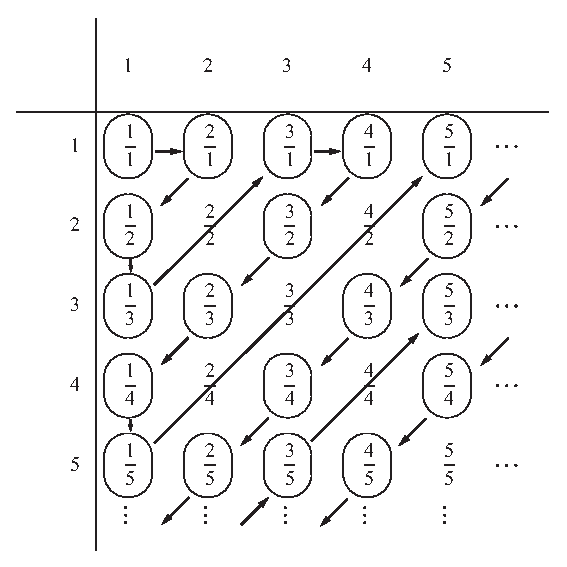
\includegraphics{figps-rationals.eps}
\caption{Counting the Positive Rational Numbers}\label{fig:positiverationals}
\end{center}
\end{figure}
The top row in Figure~\ref{fig:positiverationals} represents the numerator of the rational number, and the left column represents the denominator.  We follow the arrows in 
Figure~\ref{fig:positiverationals} to define $f\x \mathbb{N} \to \mathbb{Q}^+$.  The idea is to start in the upper left corner of the table and move to successive diagonals  as follows:
\begin{itemize}
\item We start with all fractions in which the sum of the numerator and denominator is 2 
$\left( \text{only } \dfrac{1}{1} \right)$.  So $f ( 1 ) = \dfrac{1}{1}$.

\item We next use those fractions in which the sum of the numerator and denominator is 3.  So 
$f ( 2 ) = \dfrac{2}{1}$ and $f ( 3 ) = \dfrac{1}{2}$.

\item We next use those fractions in which the sum of the numerator and denominator is 4.  So 
$f ( 4 ) = \dfrac{1}{3}$, $f ( 5 ) = \dfrac{3}{1}$.  We skipped 
$\dfrac{2}{2}$ since $\dfrac{2}{2} = \dfrac{1}{1}$.  In this way, we will ensure that the function $f$ is a one-to-one function.
\end{itemize}
We now continue with successive diagonals omitting fractions that are not in lowest terms.  This process guarantees that the function $f$ will be an injection and a surjection.  Therefore, 
$\mathbb{N} \approx \mathbb{Q}^+$ and $\text{card} ( \mathbb{Q}^+ ) = \aleph_0$.
\end{myproof}

\newpar
\note For another proof of Theorem~\ref{T:positiverationals}, see exercise~(\ref{A:Qcountable}) on page~\pageref{A:Qcountable}.

\newpar
Since $\mathbb{Q}^+$ is countable, it seems reasonable to expect that $Q$ is countable.  We will explore this soon.  On the other hand, at this point, it may also seem reasonable to ask, 
\begin{center}
``Are there any uncountable sets?''
\end{center}
The answer to this question is yes, but we will wait until the next section to prove that certain sets are uncountable.  We still have a few more issues to deal with concerning countable sets.
\endinput

\subsection*{Countably Infinite Sets}

\begin{theorem}\label{T:addonetocountable}
If $A$ is a countably infinite set, then $A \cup \left\{ x \right\}$ is a countably infinite set.
\end{theorem}
%
\begin{myproof}
Let $A$ be a  countably infinite set.  Then there exists a bijection $f\x \mathbb{N} \to A$.  Since $x$ is either in $A$ or not in $A$, we can consider two cases.

\newpar
If $x \in A$, then $A \cup \left\{ x \right\} = A$ and $A \cup \left\{ x \right\}$ is countably infinite.

\newpar
If $x \notin A$, define $g\x \mathbb{N} \to A \cup \left\{ x \right\}$ by
\begin{equation} \notag
g( n ) = 
\begin{cases}
x                        &\text{if $n = 1$} \\
f ( n - 1 )   &\text{if $n > 1$.}
\end{cases}
\end{equation}
The proof that the function $g$ is a bijection is Exercise~(\ref{exer:addonetocountable}).  Since $g$ is a bijection, we have proved that $A \cup \left\{ x \right\} \approx \N$ and hence, $A \cup \left\{ x \right\}$ is countably infinite.
\end{myproof}
%
\begin{theorem}\label{T:addfinitetocountable}
If $A$ is a countably infinite set and $B$ is a finite set, then $A \cup B$ is a countably infinite set.
\end{theorem}
%
\begin{myproof}
Exercise~(\ref{exer:addfinitetocountable}) on page~\pageref{exer:addfinitetocountable}.
\end{myproof}
%

Theorem~\ref{T:addfinitetocountable} says that if we add a finite number of elements to a countably infinite set, the resulting set is still countably infinite.  In other words, the cardinality of the new set is the same as the cardinality of the original set.  Finite sets behave very differently in the sense that if we add elements to a finite set, we will change the cardinality.  What may even be more surprising  is the result in Theorem~\ref{T:unionofcountable} that states that the union of two countably infinite (disjoint) sets is countably infinite.  The proof of this result is similar to the proof that the integers are countably infinite  (Theorem~\ref{T:ZequivtoN}).  In fact, if $A = \{a_1, a_2, a_3, \ldots \}$ and $B = \{b_1, b_2, b_3, \ldots \}$, then we can use the following diagram to help define a bijection from $\N$ to $A \cup B$.


\begin{figure}[h]
$$
\BeginTable
\BeginFormat
| c | c | c | c | c | c | c | c | c | c | c |
\EndFormat
" 1 " 2 " 3 " 4 " 5 " 6 " 7 " 8 " 9 " 10 " $\cdots$ " \\
" $\downarrow$ " $\downarrow$ " $\downarrow$ " $\downarrow$ " $\downarrow$ " $\downarrow$ " $\downarrow$ " $\downarrow$ " $\downarrow$ " $\downarrow$ " $\cdots$ "\\
" $a_1$ " $b_1$ " $a_2$ " $b_2$ " $a_3$ " $b_3$ " $a_4$ " $b_4$ " $a_5$ " $b_5$ "  $\cdots$ " \\
\EndTable
$$
\caption{A Function from $\N$ to $A \cup B$} \label{fig:functionNtoUnion}
\end{figure}


\begin{theorem}\label{T:unionofcountable}
If $A$ and $B$ are disjoint countably infinite sets,
\index{countably infinite sets!union of}%
 then $A \cup B$ is a countably infinite set.
\end{theorem}
%
\begin{myproof}
Let $A$ and $B$ be countably infinite sets and let $f\x \mathbb{N} \to A$ and 
$g\x \mathbb{N} \to B$ be bijections.  Define $h\x \mathbb{N} \to A \cup B$ by
\begin{equation} \notag
h( n ) = 
\begin{cases}
f \!\left( \dfrac{n+1}{2} \right)                        &\text{if $n$ is odd} \\
                                                       & \\
g \!\left( \dfrac{n}{2} \right)                          &\text{if $n$ is even}.
\end{cases}
\end{equation}
It is left as Exercise~(\ref{exer:unionofcountable}) on 
page~\pageref{exer:unionofcountable} to prove that the function $h$ is a bijection.
\end{myproof}

Since we can write the set of rational numbers $\Q$ as the union of the set of nonnegative rational numbers and the set of negative rational numbers, we can use the results in Theorem~\ref{T:positiverationals}, Theorem~\ref{T:addonetocountable}, and Theorem~\ref{T:unionofcountable} to prove the following theorem.

\begin{theorem}\label{T:Qiscountable}
The set $\mathbb{Q}$ of all rational numbers is countably infinite.
\end{theorem}
%
\begin{myproof}
Exercise~(\ref{exer:Qiscountable}) on page~\pageref{exer:Qiscountable}.
\end{myproof}
%\hbreak
%
\index{countably infinite sets!subsets of|(}%
In Section~\ref{S:finitesets}, we proved that any subset of a finite set is finite 
(Theorem~\ref{T:finitesubsets}).  A similar result should be expected for countable sets. We first prove that every subset of $\mathbb{N}$ is countable.  For an infinite subset $B$ of 
$\mathbb{N}$, the idea of the proof is to define a function $g\x  \mathbb{N} \to B$ by removing the elements from $B$ from smallest to the next smallest to the next smallest, and so on.  
We do this by defining the function $g$ recursively as follows:
\begin{itemize}
\item Let $g ( 1 )$ be the smallest natural number in $B$.
\item Remove $g ( 1 )$ from $B$ and let $g ( 2 )$ be the smallest natural number in \linebreak
$B - \left\{ g ( 1 ) \right\}$.
\item Remove $g ( 2 )$ and let $g ( 3 )$ be the smallest natural number in 
\linebreak
$B - \left\{ g ( 1 ), g ( 2 ) \right\}$.
\item We continue this process.  The formal recursive definition of $g\x  \mathbb{N} \to B$ is included in the proof of Theorem~\ref{T:subsetsofN}.
\end{itemize}
%
\begin{theorem}\label{T:subsetsofN}
Every subset of the natural numbers is countable.
\end{theorem}
%
\begin{myproof}
Let $B$ be a subset of $\mathbb{N}$.  If $B$ is finite, then $B$ is countable.  So we next assume that $B$ is infinite.  We will next give a recursive definition of a function 
$g\x  \mathbb{N} \to B$ and then prove that $g$ is a bijection.
\begin{itemize}
\item Let $g ( 1 )$ be the smallest natural number in $B$.
\item For each $n \in \mathbb{N}$, the set 
$B - \left\{ g ( 1 ), g ( 2 ), \ldots, g ( n ) \right\}$ is not empty since $B$ is infinite.  Define $g ( n + 1 )$ to be the smallest natural number in 
\linebreak
$B - \left\{ g ( 1 ), g ( 2 ), \ldots, g ( n ) \right\}$.
\end{itemize}
The proof that the function $g$ is a bijection is Exercise~(\ref{exer:subsetofN}) on page~\pageref{exer:subsetofN}.  
\end{myproof}
%
\begin{corollary}\label{C:subsetofcountable}
Every subset of a countable set is countable.
\end{corollary}
%
\begin{myproof}
Exercise~(\ref{exer:subsetofcountable}) on page~\pageref{exer:subsetofcountable}.
\end{myproof}
\index{countably infinite sets!subsets of|)}%

\hbreak

\endinput


\endinput



%\hrule
%

Since $\mathbb{Q}^+$ is countable, it seems reasonable to expect that $Q$ is countable.  We will explore this soon.  On the other hand, at this point, it may also seem reasonable to ask, 
\begin{center}
``Are there any uncountable sets?''
\end{center}

\begin{figure}[h]
\begin{center}
\setlength{\unitlength}{0.5cm}
\begin{picture}(20,20)
\put(4,18){1}
\put(7,18){2}
\put(10,18){3}
\put(13,18){4}
\put(16,18){5}

\put(2,15){1}
\put(2,12){2}
\put(2,9){3}
\put(2,6){4}
\put(2,3){5}

\put(0,16.5){\line(1,0){20}}
\put(3,0){\line(0,1){20}}

\put(4,15){$\dfrac{1}{1}$}
\put(7,15){$\dfrac{2}{1}$}
\put(10,15){$\dfrac{3}{1}$}
\put(13,15){$\dfrac{4}{1}$}
\put(16,15){$\dfrac{5}{1}$}
\put(18,15){$\cdots$}

\put(4.2,15.2){\oval(1.8,2.4)}
\put(7.2,15.2){\oval(1.8,2.4)}
\put(10.2,15.2){\oval(1.8,2.4)}
\put(13.2,15.2){\oval(1.8,2.4)}
\put(16.2,15.2){\oval(1.8,2.4)}

\put(4,12){$\dfrac{1}{2}$}
\put(7,12){$\dfrac{2}{2}$}
\put(10,12){$\dfrac{3}{2}$}
\put(13,12){$\dfrac{4}{2}$}
\put(16,12){$\dfrac{5}{2}$}
\put(18,12){$\cdots$}

\put(4.2,12.2){\oval(1.8,2.4)}
\put(10.2,12.2){\oval(1.8,2.4)}
\put(16.2,12.2){\oval(1.8,2.4)}

\put(4,9){$\dfrac{1}{3}$}
\put(7,9){$\dfrac{2}{3}$}
\put(10,9){$\dfrac{3}{3}$}
\put(13,9){$\dfrac{4}{3}$}
\put(16,9){$\dfrac{5}{3}$}
\put(18,9){$\cdots$}

\put(4.2,9.2){\oval(1.8,2.4)}
\put(7.2,9.2){\oval(1.8,2.4)}
\put(13.2,9.2){\oval(1.8,2.4)}
\put(16.2,9.2){\oval(1.8,2.4)}

\put(4,6){$\dfrac{1}{4}$}
\put(7,6){$\dfrac{2}{4}$}
\put(10,6){$\dfrac{3}{4}$}
\put(13,6){$\dfrac{4}{4}$}
\put(16,6){$\dfrac{5}{4}$}
\put(18,6){$\cdots$}

\put(4.2,6.2){\oval(1.8,2.4)}
\put(10.2,6.2){\oval(1.8,2.4)}
\put(16.2,6.2){\oval(1.8,2.4)}

\put(4,3){$\dfrac{1}{5}$}
\put(7,3){$\dfrac{2}{5}$}
\put(10,3){$\dfrac{3}{5}$}
\put(13,3){$\dfrac{4}{5}$}
\put(16,3){$\dfrac{5}{5}$}
\put(18,3){$\cdots$}

\put(4.2,3.2){\oval(1.8,2.4)}
\put(7.2,3.2){\oval(1.8,2.4)}
\put(10.2,3.2){\oval(1.8,2.4)}
\put(13.2,3.2){\oval(1.8,2.4)}

\put(4,1){$\vdots$}
\put(7,1){$\vdots$}
\put(10,1){$\vdots$}
\put(13,1){$\vdots$}
\put(16,1){$\vdots$}

\put(5.2,15){\vector(1,0){1}}

\put(6.5,14){\vector(-1,-1){1}}
\put(4.3,11){\vector(0,-1){.5}}

\put(5.2,10){\vector(1,1){4}}
\put(11.2,15){\vector(1,0){1}}
\put(12.5,14){\vector(-1,-1){1}}
\put(9.5,11){\vector(-1,-1){1}}
\put(6.5,8){\vector(-1,-1){1}}
\put(4.3,5){\vector(0,-1){.5}}
\put(5.2,4){\vector(1,1){10}}

\put(18.5,14){\vector(-1,-1){1}}
\put(15.5,11){\vector(-1,-1){1}}
\put(12.5,8){\vector(-1,-1){1}}
\put(9.5,5){\vector(-1,-1){1}}
\put(6.5,2){\vector(-1,-1){1}}

\put(8.5,1){\vector(1,1){1}}
\put(11.1,4.1){\vector(1,1){4}}

\put(18.5,8){\vector(-1,-1){1}}
\put(15.5,5){\vector(-1,-1){1}}
\put(12.5,2){\vector(-1,-1){1}}
\end{picture}
\caption{Counting the Positive Rational Numbers}\label{fig:positiverationals}
\end{center}
\end{figure}

\section*{Exercises \ref{S:infinitesets}}

\begin{enumerate}
\xitem State whether each of the following is true or false.
\label{exer:sec93-1}%
\begin{enumerate}
\item If a set $A$ is countably infinite, then $A$ is infinite.
\item If a set $A$ is countably infinite, then $A$ is countable.
\item If a set $A$ is uncountable, then $A$ is not countably infinite.
\item If $A \approx \mathbb{N}_k$ for some $k \in \mathbb{N}$, then $A$ is not countable.
\end{enumerate}

\item Prove that each of the following sets is countably infinite.
\label{exer:sec93-2}%
\begin{enumerate}
\item The set $F^+$ of all natural numbers that are multiples of 5
\item The set $F$ of all integers that are multiples of 5
\end{enumerate}
\begin{multicols}{2}
\begin{enumerate} \setcounter{enumii}{2}
\item $\left\{ \left. \dfrac{1}{2^k} \right| k \in \mathbb{N} \right\}$
\item $\left\{ n \in \mathbb{Z} \mid n \geq -10 \right\}$
\yitem $\mathbb{N} - \left\{ 4, 5, 6 \right\}$
\yitem $\left\{ m \in \mathbb{Z} \mid m \equiv 2 \pmod 3 \right\}$
\end{enumerate}
\end{multicols}

\item Prove part~(\ref{T:subsetisinfinite2}) of Theorem~\ref{T:subsetisinfinite}. 
\label{exer:subsetisinfinite}%

Let $A$ and $B$ be sets.  If $A$ is infinite and $A \subseteq B$, then $B$ is infinite.



\item Complete the proof of Theorem~\ref{T:addonetocountable} by proving the following:
\label{exer:addonetocountable}%

\noindent
Let $A$ be a countably infinite set and $x \notin A$.  If $f\x \mathbb{N} \to A$ is a bijection,  then $g$ is a bijection, where
$g\x \mathbb{N} \to A \cup \left\{ x \right\}$ by
\begin{equation} \notag
g( n ) = 
\begin{cases}
x                        &\text{if $n = 1$} \\
f ( n - 1 )   &\text{if $n > 1$}.
\end{cases}
\end{equation}

\xitem Prove Theorem~\ref{T:addfinitetocountable}. 
\label{exer:addfinitetocountable}%

If $A$ is a countably infinite set and $B$ is a finite set, then $A \cup B$ is a countably infinite set.

\hint  Let $\text{card} ( B ) = n$ and use a proof by induction on $n$.  
Theorem~\ref{T:addonetocountable} is the basis step.

\xitem Complete the proof of Theorem~\ref{T:unionofcountable} by proving the following: 
\label{exer:unionofcountable}%

Let $A$ and $B$ be disjoint countably infinite sets and let $f\x \mathbb{N} \to A$ and 
$g\x \mathbb{N} \to B$ be bijections.  Define $h\x \mathbb{N} \to A \cup B$ by
\begin{equation} \notag
h( n ) = 
\begin{cases}
f \!\left( \dfrac{n+1}{2} \right)                        &\text{if $n$ is odd} \\
                                                       & \\
g \!\left( \dfrac{n}{2} \right)                          &\text{if $n$ is even}.
\end{cases}
\end{equation}
Then the function $h$ is a bijection.

\xitem Prove Theorem~\ref{T:Qiscountable}.
\label{exer:Qiscountable}%

The set $\mathbb{Q}$ of all rational numbers is countable.

\hint  Use Theorem~\ref{T:addonetocountable} and Theorem~\ref{T:unionofcountable}.

\xitem Prove that if $A$ is countably infinite and $B$ is finite, then $A - B$ is countably infinite. 
\label{exer:countinf-finite}%

\item Define $f\x \mathbb{N} \times \mathbb{N} \to \mathbb{N}$ as follows:  For each 
$( m, n ) \in \mathbb{N} \times \mathbb{N}$, 
\label{exer:NxNbijection}%
\[
f ( m, n ) = 2^{m-1} (2n - 1 ).
\] 
\begin{enumerate}
\item Prove that $f$ is an injection.  \hint  If 
$f ( m, n ) = f ( s, t )$, there are three cases to consider:  $m > s$, $m < s$, and $m = s$. Use laws of exponents to prove that the first two cases lead to a contradiction.

\item Prove that $f$ is a surjection.  \hint  You may use the fact that if $y \in \mathbb{N}$, then $y = 2^k x$, where $x$ is an odd natural number and $k$ is a non-negative integer.  This is actually a consequence of the Fundamental Theorem of Arithmetic, Theorem~\ref{T:fundtheorem}.  [See Exercise~(\ref{exer:fundtheoremcons}) in Section~\ref{S:primefactorizations}.]

\item Prove that $\mathbb{N} \times \mathbb{N} \approx \mathbb{N}$ and hence that 
$\text{card} \left( \mathbb{N} \times \mathbb{N} \right) = \aleph_0$.
\end{enumerate}

\item Use Exercise~(\ref{exer:NxNbijection}) to prove that if $A$ and $B$ are countably infinite sets, then $A \times B$ is a countably infinite set.

\item Complete the proof of Theorem~\ref{T:subsetsofN} by proving that the function $g$ defined in the proof is a bijection from $\mathbb{N}$ to $B$. 
\label{exer:subsetofN}%

\hint  To prove that $g$ is an injection, it might be easier to prove that for all 
$r, s \in \mathbb{N}$, if $r \ne s$, then $g ( r ) \ne g ( s )$.  To do this, we may assume that $r < s$ since one of the two numbers must be less than the other.  Then notice that $g ( r ) \in \left\{ g( 1 ), g( 2 ), \ldots, g( s-1 ) \right\}$.

To prove that $g$ is a surjection, let $b \in B$ and notice that for some $k \in \mathbb{N}$, there will be $k$ natural numbers in $B$ that are less than $b$.

\item Prove Corollary~\ref{C:subsetofcountable}, which states that every subset of a countable set is countable. 
\label{exer:subsetofcountable}%

\hint  Let $S$ be a countable set and assume that $A \subseteq S$.  There are two cases:  $A$ is finite or $A$ is infinite.  If $A$ is infinite, let $f\x S \to \mathbb{N}$ be a bijection and define $g\x A \to f ( A )$ by $g ( x ) = f ( x )$, for each $x \in A$.

\item Use Corollary~\ref{C:subsetofcountable} to prove that the set of all rational numbers between 0 and 1 is countably infinite. 

\item \label{exer:tworationals} Let $a, b \in \mathbb{Q}$ with $a < b$. On page~\pageref{tworationals}, we proved that $c = \dfrac{a+b}{2}$ is a rational number and that $a < c < b$, which proves that here is a rational number between any two (unequal) rational numbers.
\begin{enumerate}
\item Now let  $c_1 = \dfrac{a+b}{2}$, and define $c_2 = \dfrac{c_1 + b}{2}$.  Prove that 
$c_1 < c_2 < b$ and hence, that $a < c_1 < c_2 < b$.


\item For each $k \in \mathbb{N}$, define
\[
c_{k+1} = \frac{c_k + b}{2}.
\]
Prove that for each $k \in \mathbb{N}$, $a < c_k < c_{k+1} < b$.  Use this to explain why the set 
$\left\{ c_k \mid k \in \mathbb{N} \right\}$ is an infinite set where each element is a rational number between $a$ and $b$.
\end{enumerate}
\end{enumerate}



\subsection*{Explorations and Activities}
\setcounter{oldenumi}{\theenumi}
\begin{enumerate} \setcounter{enumi}{\theoldenumi}
\item \textbf{Another Proof that $\mathbf{\Q^+}$ Is Countable}. \label{A:Qcountable} 
For this activity, it may be helpful to use the Fundamental Theorem of Arithmetic (see Theorem~\ref{T:fundtheorem} on page~\pageref{T:fundtheorem}).  Let $\Q^+$ be the set of positive rational numbers.  Every positive rational number has a unique representation as a fraction $\dfrac{m}{n}$, where $m$ and $n$ are relatively prime natural numbers.
We will now define a function $f\x  \Q^+ \to \N$ as follows:

\eighth
\noindent
If $x \in \Q^+$ and $x = \dfrac{m}{n}$, where $m, n \in \N$, $n \ne 1$ and $\gcd(m, n) = 1$, we write
\[
\begin{aligned}
m &= p_1^{\alpha_1} p_2^{\alpha_2} \cdots p_r^{\alpha_r}, \quad \text{and} \\
n &= q_1^{\beta_1} q_2^{\beta_2} \cdots q_s^{\beta_s}, 
\end{aligned}
\]
where $p_1$, $p_2$, \ldots, $p_r$ are distinct prime numbers, $q_1$, $q_2$, \ldots, $q_s$ are distinct prime numbers, and 
$\alpha_1$, $\alpha_2$, \ldots, $\alpha_r$ and $\beta_1$, $\beta_2$, \ldots, $\beta_s$ are natural numbers.    
%In addition, for each $j$ with $1 \leq j \leq r$ and for each $k$ with 
%$1 \leq k \leq s$, $p_j \ne q_k$.  
We also write $1 = 2^0$ when $m = 1$.  We then define

\[
f(x) = p_1^{2\alpha_1} p_2^{2\alpha_2} \cdots p_r^{2\alpha_r}
q_1^{2\beta_1 -1 } q_2^{2 \beta_2 - 1} \cdots q_s^{2 \beta_s - 1}.
\]

\noindent
If $x = \dfrac{m}{1}$, then we define 
$f(x) = p_1^{2\alpha_1} p_2^{2\alpha_2} \cdots p_r^{2\alpha_r} = m^2$.  

\begin{enumerate}
\item Determine $f \!\left( \dfrac{2}{3} \right)$, $f \!\left( \dfrac{5}{6} \right)$, 
$f ( 6 )$, $f ( \dfrac{12}{25} )$, 
$f \!\left( \dfrac{375}{392} \right)$, and $f \!\left( \dfrac{2^3 \cdot 11^3}{3 \cdot 5^4} \right)$.

\item If possible, find $x \in \Q^+$ such that $f(x) = 100$.

\item If possible, find $x \in \Q^+$ such that $f(x) = 12$.

\item If possible, find $x \in \Q^+$ such that $f(x) = 2^8 \cdot 3^5 \cdot 13 \cdot 17^2$.

\item Prove that the function $f$ is an injection.

\item Prove that the function $f$ is a surjection.

\item What has been proved?
\end{enumerate}
\end{enumerate}


\hbreak


\endinput





%
\section{Uncountable Sets}\label{S:uncountablesets}
%\markboth{Chapter~\ref{C:topicsinsets}. Topics in Set Theory}{\ref{S:uncountablesets}. 
%Uncountable Sets}
\setcounter{previewactivity}{0}
%
\begin{previewactivity}[\textbf{The Game of Dodge Ball}]\label{PA:dodgeball} \hfill \\
\index{Dodge Ball}%
(From \emph{The Heart of Mathematics: An Invitation to Effective Thinking} by Edward B. Burger and Michael Starbird, Key Publishing Company, \copyright 2000 by Edward B. Burger and Michael Starbird.)

Dodge Ball is a game for two players.  It is played on a game board such as the one shown in Figure~\ref{fig:dodgeball}.
\begin{figure}[h]
\begin{center}
\setlength{\unitlength}{0.5cm}
\begin{picture}(15,21)
\put(1,20){Player One's Array}
\put(1,19){\line(1,0){13}}
\put(1,17){\line(1,0){13}}
\put(1,15){\line(1,0){13}}
\put(1,13){\line(1,0){13}}
\put(1,11){\line(1,0){13}}
\put(1,9){\line(1,0){13}}
\put(1,7){\line(1,0){13}}

\put(1,7){\line(0,1){12}}
\put(2,7){\line(0,1){12}}
\put(4,7){\line(0,1){12}}
\put(6,7){\line(0,1){12}}
\put(8,7){\line(0,1){12}}
\put(10,7){\line(0,1){12}}
\put(12,7){\line(0,1){12}}
\put(14,7){\line(0,1){12}}

\put(1.3,17.5){1}
\put(1.3,15.5){2}
\put(1.3,13.5){3}
\put(1.3,11.5){4}
\put(1.3,9.5){5}
\put(1.3,7.5){6}

\put(1,5){Player Two's Row}
\put(2,4){\line(1,0){12}}
\put(2,3){\line(1,0){12}}
\put(2,1){\line(1,0){12}}

\put(2,1){\line(0,1){3}}
\put(4,1){\line(0,1){3}}
\put(6,1){\line(0,1){3}}
\put(8,1){\line(0,1){3}}
\put(10,1){\line(0,1){3}}
\put(12,1){\line(0,1){3}}
\put(14,1){\line(0,1){3}}

\put(2.8,3.3){1}
\put(4.8,3.3){2}
\put(6.8,3.3){3}
\put(8.8,3.3){4}
\put(10.8,3.3){5}
\put(12.8,3.3){6}

\put(0,21){\line(1,0){15}}
\put(0,0){\line(1,0){15}}
\put(0,0){\line(0,1){21}}
\put(15,0){\line(0,1){21}}
\end{picture}
\caption{Game Board for Dodge Ball}\label{fig:dodgeball}
\end{center}
\end{figure}
Player One has a 6 by 6 array to complete and Player Two has a 1 by 6 row to complete.  Each player has six turns as described next.
\begin{itemize}
\item Player One begins by filling in the first horizontal row of his or her table with a sequence of six X's and O's, one in each square in the first row.

\item Then Player Two places either an X or an O in the first box of his or her row.  At this point, Player One has completed the first row and Player Two has filled in the first box of his or her row with one letter.

\item The game continues with Player One completing a row with six letters (X's and O's), one in each box of the next row followed by Player Two writing one letter (an X or an O) in the next box of his or her row.  The game is completed when Player One has completed all six rows and Player Two has completed all six boxes in his or her row.
\end{itemize}

\newpar
\textbf{Winning the Game}
\begin{itemize}
\item Player One wins if any horizontal row in the 6 by 6 array is identical to the row that Player Two created.  (Player One matches Player Two.)

\item Player Two wins if Player Two's row of six letters is different than each of the six rows produced by Player One.  (Player Two ``dodges'' Player One.)
\end{itemize}
There is a winning strategy for one of the two players.  This means that there is plan by which one of the two players will always win.  Which player has a winning strategy?  Carefully describe this winning strategy.


\newpar
\textbf{Applying the Winning Strategy to Lists of Real Numbers} \\
Following is a list of real numbers between 0 and 1.  Each real number is written as a decimal number.
\begin{align*}
a_1 &= 0.1234567890   &  a_6 &= 0.0103492222 \\
a_2 &= 0.3216400000   &  a_7 &= 0.0011223344 \\
a_3 &= 0.4321593333   &  a_8 &= 0.7077700022 \\
a_4 &= 0.9120930092   &  a_9 &= 0.2100000000 \\
a_5 &= 0.0000234102   & a_{10} &= 0.9870008943 
\end{align*}
Use a method similar to the winning strategy in the game of Dodge Ball to write a real number (in decimal form) between 0 and 1 that is not in this list of 10 numbers.

\begin{enumerate}
  \item Do you think your method could be used for any list of 10 real numbers between 0 and 1 if the goal is to write a real number between 0 and 1 that is not in the list?
  \item Do you think this method could be extended to a list of 20 different real numbers?  To a list of 50 different real numbers?
  \item Do you think this method could be extended to a countably infinite list of real numbers?
\end{enumerate}

\end{previewactivity}
\hbreak

\endinput

\begin{previewactivity}[\textbf{Functions from a Set to Its Power Set}]\label{PA:powerset} \hfill \\
Let $A$ be a set.  In Section~\ref{S:setoperations}, we defined the \textbf{power set}
\index{power set}% 
$\mathcal{P} ( A )$ of $A$ to be the set of all subsets of $A$.  This means that
\begin{center}
$X \in \mathcal{P} ( A )$ if and only if $X \subseteq A$.
\end{center}
%
Theorem~\ref{T:powerset} in Section~\ref{S:setoperations} states that if a set $A$ has $n$ elements, then $A$ has $2^n$ subsets or that $\mathcal{P} ( A )$ has 
$2^n$ elements.  Using our current notation for cardinality, this means that
%
\begin{center}
if $\text{card} ( A ) = n$, then 
$\text{card} ( \mathcal{P} ( A ) ) = 2^n$.
\end{center}
%
(The proof of this theorem was Exercise~(\ref{exer:powerset}) on page~\pageref{exer:powerset}.)
%\begin{enumerate}
%\item Determine the power set of each of the following sets:
%\begin{multicols}{2}
%\begin{enumerate}
%\item $A = \left\{a, b \right\}$
%\item $B = \left\{a, b, c \right\}$
%\end{enumerate}
%\end{multicols}
%\end{enumerate}
%

We are now going to define and explore some functions from a set $A$ to its power set 
$\mathcal{P} ( A )$.  This means that the input of the function will be an element of $A$ and the output of the function will be a subset of $A$.

\begin{enumerate} 
\item Let $A = \left\{1, 2, 3, 4 \right\}$.  Define $f\x A \to \mathcal{P} ( A )$ by
%
\begin{multicols}{2}
$f ( 1 ) = \left\{ 1, 2, 3 \right\}$

$f ( 2 ) = \left\{ 1, 3, 4 \right\}$

$f ( 3 ) = \left\{ 1, 4 \right\}$

$f ( 4 ) = \left\{ 2, 4 \right\}$.
\end{multicols}
%
\begin{enumerate}
\item Is $1 \in f ( 1 )$?  Is $2 \in f ( 2 )$? Is 
$3 \in f ( 3 )$?  Is $4 \in f ( 4 )$?

\item Determine $S = \left\{ x \in A \mid x \notin f ( x ) \right\}$.

\item Notice that $S \in \mathcal{P} ( A )$.  Does there exist an element $t$ in $A$ such that $f ( t ) = S$?  That is, is $S \in \text{range} ( f )$?
 
\end{enumerate}

\item Let $A = \left\{1, 2, 3, 4 \right\}$.  Define $f\x A \to \mathcal{P} ( A )$ by 
%
\begin{center}
$f ( x ) = A - \left\{ x \right\}$ for each $x \in A$.
\end{center}
%
\begin{multicols}{2}
\begin{enumerate}
\item Determine $f ( 1 )$.  Is $1 \in f ( 1 )$?
\item Determine $f ( 2 )$.  Is $2 \in f ( 2 )$?
\item Determine $f ( 3 )$.  Is $3 \in f ( 3 )$?
\item Determine $f ( 4 )$.  Is $4 \in f ( 4 )$?
\end{enumerate}
\end{multicols}
%
\begin{enumerate} \setcounter{enumii}{4}
\item Determine $S = \left\{ x \in A \mid x \notin f ( x ) \right\}$.

\item Notice that $S \in \mathcal{P} ( A )$.  Does there exist an element $t$ in $A$ such that $f ( t ) = S$?  That is, is $S \in \text{range} ( f )$?
\end{enumerate}
%
\item Define $f\x \mathbb{N} \to \mathcal{P} ( \mathbb{N} )$ by
%
\begin{center}
$f ( n ) = \mathbb{N} - \left\{n^2, n^2-2n \right\}$, for each $n \in \mathbb{N}$.
\end{center}
%
\begin{enumerate}
\item Determine $f ( 1 )$, $f ( 2 )$, $f ( 3 )$, and 
$f ( 4 )$.  In each of these cases, determine if $k \in f ( k )$.
%
\item Prove that if $n > 3$, then $n \in f ( n )$.  \hint  Prove that if $n >3$, then 
$n^2 > n$ and $n^2 - 2n >n$.

\item Determine $S = \left\{ x \in \mathbb{N} \mid x \notin f ( x ) \right\}$.

\item Notice that $S \in \mathcal{P} ( \mathbb{N} )$.  Does there exist an element $t$ in $\mathbb{N}$ such that $f ( t ) = S$?  That is, is 
$S \in \text{range} ( f )$?

\end{enumerate}
\end{enumerate}
\end{previewactivity}
%\hbreak

\endinput



%
We have seen examples of sets that are countably infinite, but we have not yet seen an example of an infinite set that is uncountable.  We will do so in this section.  The first example of an uncountable set will be the open interval of real numbers $( 0, 1 )$.  The proof that this interval is uncountable uses a method similar to the winning strategy for Player Two in the game of Dodge Ball from \typeu Activity~\ref*{PA:dodgeball}.  Before considering the proof, we need to state an important result about decimal expressions for real numbers.

\subsection*{Decimal Expressions for Real Numbers}
\index{decimal expression!for a real number}%

In its decimal form, any real number $a$ in the interval $( 0, 1 )$ can be written as
$a = 0.a_1 a_2 a_3 a_4 \ldots ,$ where each $a_i$ is an integer with $0 \leq a_i \leq 9$.  For example,
\[
\frac{5}{12} = 0.416666 \ldots.
\]
We often abbreviate this as $\dfrac{5}{12} = 0.41 \overline{6}$ to indicate that the $6$ is repeated.  We can also repeat a block of digits.  For example, 
$\dfrac{5}{26} = 0.19 \overline{230769}$ to indicate that the block 230769 repeats.  That is, 
\[
\frac{5}{26} = 0.19230769230769230769 \ldots.
\]
There is only one situation in which a real number can be represented as a decimal in more than one way.  A decimal that ends with an infinite string of 9's is equal to one that ends with an infinite string of 0's.  For example, $0.3199999 \ldots$ represents the same real number as 
$0.3200000 \ldots .$  Geometric series can be used to prove that a decimal that ends with an infinite string of 9's is equal to one that ends with an infinite string of 0's, but we will not do so here.

\begin{defbox}{normalized}{A decimal representation of a real number $a$ is in \textbf{normalized form}
\index{decimal expression!normalized form}%
\index{normalized form!of a decimal expression}%
\label{normalizedform}%
 provided that there is no natural number $k$ such that for all natural numbers $n$ with $n > k$, $a_n = 9$.  That is, the decimal representation of $a$ is in normalized form if and only if it does not end with an infinite string of 9's.}
\end{defbox}

\newpar
One reason the normalized form is important is the following theorem (which will not be proved here).
\begin{theorem} \label{T:normalized} Two decimal numbers in normalized form are equal if and only if they have identical digits in each decimal position.
\end{theorem}

\endinput

\subsection*{Uncountable Subsets of $\boldsymbol{\mathbb{R}}$}
In the proof that follows, we will use only the normalized form for the decimal representation of a real number in the interval $( 0, 1 )$.
%\hbreak
%
\begin{theorem}\label{T:uncountableinterval}
The open interval $( 0, 1 )$ is an uncountable set.
\end{theorem}
%
\begin{myproof}
Since the interval $( 0, 1 )$ contains the infinite subset 
$\left\{\dfrac{1}{2}, \dfrac{1}{3}, \dfrac{1}{4}, \ldots \,\right\}$, we can use 
Theorem~\ref{T:subsetisinfinite}, to conclude that $( 0, 1 )$ is an infinite set.  So $( 0, 1 )$ is either countably infinite or uncountable.  We will prove that $( 0, 1 )$ is uncountable by proving that any function from $\N$ to $(0, 1)$ is not a surjection, and hence, there is no bijection from $\N$ to  $(0, 1)$.

So suppose that $f\x \mathbb{N} \to ( 0, 1 )$ is a function.  We will show that $f$ is not a surjection by showing that there exists an element in 
$( 0, 1 )$ that cannot be in the range of $f$.  Writing the images of the elements of 
$\mathbb{N}$ in normalized form, we can write
\[
\begin{aligned}
f ( 1 ) &= 0.a_{1 1} a_{1 2} a_{1 3} a_{1 4} a_{1 5} \ldots \\
f ( 2 ) &= 0.a_{2 1} a_{2 2} a_{2 3} a_{2 4} a_{2 5} \ldots \\
f ( 3 ) &= 0.a_{3 1} a_{3 2} a_{3 3} a_{3 4} a_{3 5} \ldots \\
f ( 4 ) &= 0.a_{4 1} a_{4 2} a_{4 3} a_{4 4} a_{4 5} \ldots \\
f ( 5 ) &= 0.a_{5 1} a_{5 2} a_{5 3} a_{5 4} a_{5 5} \ldots \\
                   & \vdots \\
f ( n ) &= 0.a_{n 1} a_{n 2} a_{n 3} a_{n 4} a_{n 5} \ldots \\
                   & \vdots \\
\end{aligned}
\]
Notice the use of the double subscripts. The number $a_{i j}$ is the $j^\text{th}$ digit to the right of the decimal point in the normalized decimal representation of $f ( i )$.

We will now construct a real number $b = 0.b_1 b_2 b_3 b_4 b_5 \ldots$ in $( 0, 1 )$ and in normalized form that is not in this list.  

\vskip6pt
\noindent
%\emph{Informal Side Note}:  
\note The idea is to start in the upper left corner and move down the diagonal in a manner similar to the winning strategy for Player Two in the game in 
\typeu Activity~\ref*{PA:dodgeball}.  At each step, we choose a digit that is not equal to the diagonal digit.
\vskip6pt

Start with $a_{1 1}$ in $f ( 1 )$.  We want to choose $b_1$ so that $b_1 \ne 0$, 
$b_1 \ne a_{1 1}$, and $b_1 \ne 9$. (To ensure that we end up with a decimal that is in normalized form, we make sure that each digit is not equal to 9.)  We then repeat this process with $a_{2 2}$, $a_{3 3}$, 
$a_{4 4}$, $a_{5 5}$, and so on.  So we let $b$ be the real number 
$b = 0.b_1 b_2 b_3 b_4 b_5 \ldots ,$ where for each $k \in \mathbb{N}$
\begin{equation} \notag
b_k = 
\begin{cases}
3         &\text{if $a_{k k} \ne 3$} \\
5         &\text{if $a_{k k} = 3$.}
\end{cases}
\end{equation}

\noindent
(The choice of 3 and 5 is arbitrary.  Other choices of distinct digits will also work.)

Now for each $n \in \mathbb{N}$, $b \ne f ( n )$ since $b$ and $f ( n )$ are in normalized form and $b$ and $f ( n )$ differ in the $n${th} decimal place.  Therefore, $f$ is not a surjection.  This proves that any function from $\mathbb{N}$ to $( 0, 1 )$ is not a surjection and hence, there is no bijection from $\mathbb{N}$ to $( 0, 1 )$.  Therefore, 
$( 0, 1 )$ is not countably infinite and hence must be an uncountable set.
\end{myproof}
\hbreak
%
\begin{prog} [\textbf{Dodge Ball and Cantor's Diagonal Argument}]\label{prog:diagonal} \hfill \\
The proof of Theorem~\ref{T:uncountableinterval} is often referred to as \textbf{Cantor's diagonal argument}.
\index{Cantor's diagonal argument}%
  It is named after the mathematician Georg Cantor, who first published the proof in 1874.  Explain the connection between the winning strategy for Player Two in Dodge Ball
\index{Dodge Ball}%
 (see \typeu Activity~\ref*{PA:dodgeball})  and the proof of Theorem~\ref{T:uncountableinterval} using Cantor's diagonal argument.
\end{prog}
\hbreak
%
The open interval $( 0, 1 )$ is our first example of an uncountable set.  The cardinal number of $( 0, 1 )$ is defined to be $\boldsymbol{c}$, 
\label{sym:continuum}% 
which stands for 
\textbf{the cardinal number of the continuum}.
\index{continuum}%
  So the two infinite cardinal numbers we have seen are $\aleph_0$ for countably infinite sets and $\boldsymbol{c}$.

\begin{defbox}{cardinalityc}{A set $A$ is said to have \textbf{cardinality}
\index{cardinality}%
\index{cardinality!$\boldsymbol{c}$}%
%\index{$\boldsymbol{c}$}%
  $\boldsymbol{c}$ provided that $A$ is equivalent to $( 0, 1 )$.  In this case, we write 
$\text{card} ( A ) = \boldsymbol{c}$ and say that the cardinal number of $A$ is 
$\boldsymbol{c}$.}
\end{defbox}

\noindent
The proof of Theorem~\ref{T:openintervals} is included in Progress Check~\ref{prog:openintervals}.

\begin{theorem}\label{T:openintervals}
Let $a$ and $b$ be real numbers with $a < b$.  The open interval $( a, b )$ is uncountable and has cardinality $\boldsymbol{c}$.
\end{theorem}
%
\begin{prog}[\textbf{Proof of Theorem~\ref{T:openintervals}}]\label{prog:openintervals} \hfill
\begin{enumerate}
\item In Part~(\ref{A:equivsets4}) of Progress Check~\ref{prog:equivsets}, we proved that if 
$b \in \R$ and $b > 0$, then the open interval $( 0, 1 )$ is equivalent to the open interval $( 0, b )$.  Now let $a$ and $b$ be real numbers with $a < b$.  Find a function 
\[
f\x  ( 0, 1 ) \to ( a, b )
\]
that is a bijection and conclude that the open interval $( 0, 1) \approx ( a, b )$.

\hint Find a linear function that passes through the points $( 0, a )$ and 
$( 1, b )$.  Use this to define the function $f$.  Make sure you prove that this function $f$ is a bijection.

\item Let $a, b, c, d$ be real numbers with $a < b$ and $c < d$.  Prove that the open interaval $( a, b )$ is equivalent to the open interval $( c, d )$.
\end{enumerate}
\end{prog}
\hbreak
%
\begin{theorem}\label{T:realsuncount}
The set of real numbers $\mathbb{R}$ is uncountable and has cardinality $\boldsymbol{c}$.
\end{theorem}
%
\begin{myproof}
Let $f\x  \left( -\dfrac{\pi}{2}, \dfrac{\pi}{2} \right) \to \mathbb{R}$ be defined by 
$f ( x ) = \tan x$, for each $x \in \mathbb{R}$.  The function $f$ is a bijection and, hence, 
$\left(-\dfrac{\pi}{2}, \dfrac{\pi}{2} \right) \approx \mathbb{R}$.  So by 
Theorem~\ref{T:openintervals}, $\mathbb{R}$ is uncountable and has cardinality $\boldsymbol{c}$.
\end{myproof}

\endinput

\subsection*{Cantor's Theorem}
\index{Cantor's Theorem}

We have now seen two different infinite cardinal numbers, $\aleph_0$ and $\boldsymbol{c}$.  It can seem surprising that there is more than one infinite cardinal number.  A reasonable question at this point is, ``Are there any other infinite cardinal numbers?''  The astonishing answer is that there are, and in fact, there are infinitely many different infinite cardinal numbers.  The basis for this fact is the following theorem, which states that a set is not equivalent to its power set.  The proof is  due to Georg Cantor (1845--1918),
\index{Cantor, Georg}%
and the idea for this proof was explored in \typeu Activity~\ref*{PA:powerset}. The basic idea of the proof is to prove that any function from a set $A$ to its power set cannot be a surjection.

\begin{theorem}[\textbf{Cantor's Theorem}]\label{T:cantor}
For every set $A$, $A$ and $\mathcal{P} ( A )$ do not have the same cardinality.
\end{theorem}
%
\begin{myproof}
Let $A$ be a set.  If $A = \emptyset$, then 
$\mathcal{P} ( A ) = \left\{ \emptyset \right\}$, which has cardinality 1.  Therefore, 
$\emptyset$ and $\mathcal{P} ( \emptyset )$ do not have the same cardinality.

Now suppose that $A \ne \emptyset$, and let $f\x  A \to \mathcal{P} ( A )$.  We will show that $f$ cannot be a surjection, and hence there is no bijection from $A$ to 
$\mathcal{P} ( A )$.  This will prove that $A$ is not equivalent to 
$\mathcal{P} ( A )$.  Define
\[
S = \left\{ x \in A \mid x \notin f ( x ) \right\}.
\]
Assume that there exists a $t$ in $A$ such that $f ( t ) = S$.  Now, either $t \in S$ or $t \notin S$.

\begin{itemize}
\item If $t \in S$, then $t \in \left\{ x \in A \mid x \notin f ( x ) \right\}$.  By the definition of $S$, this means that $t \notin f ( t )$.  However, 
$f ( t ) = S$ and so we conclude that $t \notin S$.  But now we have $t \in S$ and $t \notin S$.  This is a contradiction.

\item If $t \notin S$, then $t \notin \left\{ x \in A \mid x \notin f ( x ) \right\}$.  By the definition of $S$, this means that $t \in f ( t )$.  However, 
$f ( t ) = S$ and so we conclude that $t \in S$.  But now we have $t \notin S$ and $t \in S$.  This is a contradiction.
\end{itemize}
So in both cases we have arrived at a contradiction.  This means that there does not exist a 
$t$ in $A$ such that $f ( t ) = S$.  Therefore, any function from $A$ to 
$\mathcal{P} ( A )$ is not a surjection and hence not a bijection.  Hence, $A$ and 
$\mathcal{P} ( A )$ do not have the same cardinality. 
\end{myproof}
%\hbreak
%
\begin{corollary}\label{C:cantor}
$\mathcal{P} ( \mathbb{N} )$ is an infinite set that is not countably infinite.
\end{corollary}
%
\begin{myproof}
Since $\mathcal{P} ( \mathbb{N} )$ contains the infinite subset 
$\left\{ \left\{ 1 \right\}, \left\{ 2 \right\}, \left\{ 3 \right\} \ldots \,\right\}$, we can use 
Theorem~\ref{T:subsetisinfinite}, to conclude that $\mathcal{P} ( \mathbb{N} )$ is an infinite set.  By Cantor's Theorem (Theorem~\ref{T:cantor}), $\mathbb{N}$ and 
$\mathcal{P} ( \mathbb{N} )$ do not have the same cardinality.  Therefore, 
$\mathcal{P} ( \mathbb{N} )$ is not countable and hence is an uncountable set.
\end{myproof}
%
\subsection*{Some Final Comments about Uncountable Sets}
\begin{enumerate}
\item We have now seen that any open interval of real numbers is uncountable and has cardinality \
$\boldsymbol{c}$.  In addition, $\mathbb{R}$ is uncountable and has cardinality $\boldsymbol{c}$.  Now, Corollary~\ref{C:cantor} tells us that $\mathcal{P} ( \mathbb{N} )$ is uncountable.  A question that can be asked is, 
\begin{center}
``Does $\mathcal{P} ( \mathbb{N} )$ have the same cardinality as $\mathbb{R}$?''
\end{center}
The answer is yes, although we are not in a position to prove it yet.  A proof of this fact uses the following theorem, which is known as the Cantor-Schr\"{o}der-Bernstein Theorem.
\label{sec94:comment1}%
\end{enumerate}

\begin{theorem}[\textbf{Cantor-Schr\"{o}der-Bernstein}]\label{T:bernstein}
Let $A$ and $B$ be sets.  If there exist injections $f\x A \to B$ and $g\x B \to A$, then 
$A \approx B$.
\end{theorem}
\index{Cantor-Schr\"{o}der-Bernstein Theorem}%


In the statement of this theorem, notice that it is not required that the function $g$ be the inverse of the function $f$.  We will not prove the Cantor-Schr\"{o}der-Bernstein Theorem here.  
The following items will show some uses of this important theorem. 
%but a proof is given in Section~\ref{S:CSBproof}.  
%The following item will indicate another use of this theorem.

\begin{enumerate} \setcounter{enumi}{1}
\item The Cantor-Schr\"{o}der-Bernstein Theorem can also be used to prove that the closed interval 
$[ 0, 1 ]$ is equivalent to the open interval $( 0, 1 )$.  
See Exercise~(\ref{exer:closedinterval}) on page~\pageref{exer:closedinterval}.

\item Another question that was posed earlier is,
\begin{center}
``Are there other infinite cardinal numbers other than $\aleph_0$ and $\boldsymbol{c}$?''
\end{center}
Again, the answer is yes, and the basis for this is Cantor's Theorem (Theorem~\ref{T:cantor}).
We can start with $\text{card} ( \mathbb{N} ) = \aleph_0$.  We then define the following infinite cardinal numbers:
\begin{multicols}{2}
\begin{list}{}
\item $\text{card} ( \mathcal{P} ( \mathbb{N} ) ) = \alpha_1$.

\item $\text{card} ( \mathcal{P} ( \mathcal{P} ( \mathbb{N} ) ) ) = \alpha_2$.

\item $\text{card} ( \mathcal{P} ( \mathcal{P} ( \mathcal{P} ( \mathbb{N} ) ) ) ) = \alpha_3$. 
\label{sec94:comment3}%
\item $\vdots$
\end{list}
\end{multicols}

%\begin{multicols}{2}
%\begin{list}{}
%\item $\text{card} ( \mathcal{P} ( \mathbb{N} ) )$.
%
%\item $\text{card} ( \mathcal{P} ( \mathcal{P} ( \mathbb{N} ) ) )$.
%
%\item $\text{card} ( \mathcal{P} ( \mathcal{P} ( \mathcal{P} ( \mathbb{N} ) ) ) )$. 
%\label{sec94:comment3}%
%
%\item $\vdots$
%\end{list}
%\end{multicols}
Cantor's Theorem tells us that these are all different cardinal numbers, and so we are just using the lowercase Greek letter $\alpha$ (alpha) to help give names to these cardinal numbers.  In fact, although we will not define it here, there is a way to ``order'' these cardinal numbers in such a way that 
%\[
%\aleph_0 < \text{card} ( \mathcal{P} ( \mathbb{N} ) ) < \text{card} ( \mathcal{P} ( \mathcal{P} ( \mathbb{N} ) ) ) < \aleph_3 < \cdots.
%\]
\[
\aleph_0 < \alpha_1 < \alpha_2 < \alpha_3 < \cdots.
\]
Keep in mind, however, that even though these are different cardinal numbers, Cantor's Theorem does not tell us that these are the only cardinal numbers.

\item In Comment~(\ref{sec94:comment1}), we indicated that 
$\mathcal{P} ( \mathbb{N} )$ and $\mathbb{R}$ have the same cardinality.  Combining this with the notation in Comment~(\ref{sec94:comment3}), this means that 
\[
\alpha_1 = \boldsymbol{c}.
\]
However, this does not necessarily mean that $\boldsymbol{c}$ is the ``next largest'' cardinal number after 
$\aleph_0$.  A reasonable question is, ``Is there an infinite set with cardinality between 
$\aleph_0$ and $\boldsymbol{c}$?''  Rewording this in terms of the real number line, the question is, ``On the real number line, is there an infinite set of points that is not equivalent to the entire line and also not equivalent to the set of natural numbers?''  This question was asked by Cantor, but he was unable to find any such set.  He conjectured that no such set exists.  That is, he conjectured that $\boldsymbol{c}$ is really the next cardinal number after 
$\aleph_0$.  This conjecture has come to be known as the \textbf{Continuum Hypothesis}.
\index{Continuum Hypothesis}%
Stated somewhat more formally, the Continuum Hypothesis is
\begin{center}
There is no set $X$ such that $\aleph_0 < \text{card} ( X ) < \boldsymbol{c}$.
\end{center}
The question of whether the Continuum Hypothesis is true or false is one of the most famous problems in modern mathematics.  

Through the combined work of Kurt G\"{o}del
\index{G\"{o}del, Kurt}%
 in the 1930s and Paul Cohen
\index{Cohen, Paul}%
 in 1963, it has been proved that the Continuum Hypothesis cannot be proved or disproved from the standard axioms of set theory.  This means that either the Continuum Hypothesis or its negation can be added to the standard axioms of set theory without creating a contradiction.

\end{enumerate}
\hbreak 


\endinput



%\vskip6pt

%
%




\endinput

%\newpage
\section*{Exercises \ref{S:uncountablesets}}

\begin{enumerate}
\item Use an appropriate bijection to prove that each of the following sets has cardinality $\boldsymbol{c}$. 
\label{exer:sec94-1}%
\begin{multicols}{2}
\begin{enumerate}
\yitem $( 0, \infty )$
\yitem $( a, \infty )$, for any $a \in \mathbb{R}$
\item $\mathbb{R} - \left\{ 0 \right\}$
\item $\mathbb{R} - \left\{ a \right\}$, for any $a \in \mathbb{R}$
\end{enumerate}
\end{multicols}

\xitem Is the set of irrational numbers countable or uncountable? Prove that your answer is correct. 
\label{exer:irrationaluncount}%

\xitem Prove that if $A$ is uncountable and $A \subseteq B$, then $B$ is uncountable.
\label{exer:supersetofuncount}%

\xitem Do two uncountable sets always have the same cardinality?  Justify your conclusion. \label{exer93:uncountablesets}


\item Let  $C$  be the set of all infinite sequences, each of whose entries is the digit 0 or the digit 1.  For example,
\[
\begin{aligned}
\left( 1, 0, 1, 0, 1, 0, 1, 0, \ldots \right) &\in C; \\
\left( 0, 1, 0, 1, 1, 0, 1, 1, 1, 0, 1, 1, 1, 1, \ldots \right) &\in C; \\
\left( 2, 1, 0, 1, 1, 0, 1, 1, 1, 0, 1, 1, 1, 1, \ldots \right) &\notin C.
\end{aligned}
\]
Is the set  $C$  a countable set or an uncountable set?  Justify your conclusion.


\item The goal of this exercise is to use the Cantor-Schr\"{o}der-Bernstein Theorem to prove that the cardinality of the closed interval $[ 0, 1 ]$ is $\boldsymbol{c}$.
\label{exer:closedinterval}%

\begin{enumerate}
\item Find an injection $f\x  ( 0, 1 ) \to [ 0, 1 ]$.

\item Find an injection $h\x  [ 0, 1 ] \to ( -1, 2 )$.

\item Use the fact that $( -1, 2 ) \approx ( 0, 1 )$ to prove that there exists an injection 
$g\x  [ 0, 1 ] \to ( 0, 1 )$.  (It is only necessary to prove that the injection $g$ exists.  It is not necessary to determine a specific formula for 
$g ( x )$.)  

\note  Instead of doing Part~(b) as stated, another approach is to find an injection 
$k \x [0, 1] \to (0, 1)$.  Then, it is possible to skip Part~(c) and go directly to Part~(d).

\item Use the Cantor-Schr\"{o}der-Bernstein Theorem to conclude that \linebreak
$[ 0, 1 ] \approx ( 0, 1 )$ and hence that the cardinality of 
$[ 0, 1 ]$ is $\boldsymbol{c}$.
\end{enumerate}

\item In Exercise~(\ref{exer:closedinterval}), we proved that the closed interval $[ 0, 1 ]$ is uncountable and has cardinality $\boldsymbol{c}$.  Now let $a, b \in \mathbb{R}$ with $a < b$.  Prove that 
$[ a, b ] \approx [ 0, 1 ]$ and hence that $[ a, b ]$ is uncountable and has cardinality $\boldsymbol{c}$.



\item Is the set of all finite subsets of $\N$ countable or uncountable? Let $F$ be the set of all finite subsets of $\N$.  Determine the cardinality of the set $F$.

\eighth
\noindent
Consider defining a function $f:F \to \N$ that produces the following.
\begin{itemize}
  \item If $A = \{1, 2, 6 \}$, then $f(A) = 2^1 3^2 5^6$.
  \item If $B = \{3, 6 \}$, then $f(B) = 2^3 3^6$.
  \item If $C = \left\{ m_1, m_2, m_3, m_4 \right\}$ with $m_1 < m_2 < m_3 < m_4$, then 
           $f(C) = 2^{m_1} 3^{m_2} 5^{m_3} 7^{m_4}$.
\end{itemize}
It might be helpful to use the Fundamental Theorem of Arithmetic on page~\pageref{T:fundtheorem} and to denote the set of all primes as  $P = \left\{ p_1, p_2, p_3, p_4, \ldots \right\}$ with $p_1 < p_2 < p_3 < p_4 \cdots$.  Using the sets $A$, $B$, and $C$ defined above, we would then write
\[
f(A) = p_1^1 p_2^2 p_3^6, \quad f(B) = p_1^3 p_2^6, \quad \text{and} \quad f(C) = p_1^{m_1} p_2^{m_2} p_3^{m_3} p_4^{m_4}.
\]

\item In Exercise~(\ref{exer:irrationaluncount}), we showed that the set of irrational numbers is uncountable.  However, we still do not know the cardinality of the set of irrational numbers.  Notice that we can use $\Q^c$ to stand for the set of irrational numbers.

\begin{enumerate}
\item Construct a function $f\x \Q^c \to \R$ that is an injection.
\end{enumerate}
We know that any real number $a$ can be represented in decimal form as follows:
\[
a = A.a_1 a_2 a_3 a_4 \cdots a_n \cdots ,
\]
where $A$ is an integer and the decimal part $( 0.a_1 a_2 a_3 a_4 \cdots )$ is in normalized form.  (See page~\pageref{normalizedform}.)  We also know that the real number $a$ is an irrational number if and only $a$ has an infinite non-repeating decimal expansion.  We now associate with $a$ the real number
\setcounter{equation}{0}
\begin{equation}\label{exer:irrationalsuncount}
A.a_1 0 a_2 1 1 a_3 0 0 0 a_4 1 1 1 1 a_5 0 0 0 0 0 a_6 1 1 1 1 1 1 \cdots .
\end{equation}
Notice that to construct the real number in (\ref{exer:irrationalsuncount}), we started with the decimal expansion of $a$, inserted a 0 to the right of the first digit after the decimal point, inserted two 1's to the right of the second digit to the right of the decimal point, inserted three 0's to the right of the third digit to the right of the decimal point, and so on.

\begin{enumerate} \setcounter{enumii}{1}
\item Explain why the real number in (\ref{exer:irrationalsuncount}) is an irrational number.
\item Use these ideas to construct a function $g\x \R \to \Q^c$ that is an injection.
\item What can we now conclude by using the Cantor-Schr\"{o}der-Bernstein Theorem?
\end{enumerate}

\item Let $J$ be the unit open interval.  That is, $J = \left\{ x \in \R \mid 0 < x < 1 \right\}$ and let $S = \left\{ (x, y) \in \R \times \R \mid 0 < x < 1 \text{ and } 0 < y < 1 \right\}$.  We call $S$ the unit open square.  We will now define a function $f$ from $S$ to $J$.  Let 
$(a, b) \in S$ and write the decimal expansions of $a$ and $b$ in normalized form as
\begin{align*}
a &= 0.a_1 a_2 a_3 a_4 \cdots a_n \cdots \\
b &= 0.b_1 b_2 b_3 b_4 \cdots b_n \cdots .
\end{align*}
We then define $f(a, b) = 0.a_1 b_1 a_2 b_2 a_3 b_3 a_4 b_4 \cdots a_n b_n \cdots$.
\begin{enumerate}
\item Determine the values of $f ( 0.3, 0.625 )$, $f \!\left( \dfrac{1}{3}, \dfrac{1}{4} \right)$, and $f \!\left( \dfrac{1}{6}, \dfrac{5}{6} \right)$.

\item If possible, find $(x, y) \in S$ such that $f ( x, y ) = 0.2345$.

\item If possible, find $(x, y) \in S$ such that $f ( x, y ) = \dfrac{1}{3}$.

\item If possible, find $(x, y) \in S$ such that $f ( x, y ) = \dfrac{1}{2}$.

\item Explain why the function $f\x S \to J$ is an injection but is not a surjection.

\item Use the Cantor-Schr\"{o}der-Bernstein Theorem to prove that the cardinality of the unit open square $S$ is equal to $\boldsymbol{c}$. If this result seems surprising, you are in good company.  In a letter written in 1877 to the mathematician Richard Dedekind describing this result that he had discovered, Georg Cantor wrote, ``I see it but I do not believe it.''
\end{enumerate}
 
\end{enumerate}

\subsection*{Explorations and Activities}
\setcounter{oldenumi}{\theenumi}
\begin{enumerate} \setcounter{enumi}{\theoldenumi}
\item \textbf{The Closed Interval $\boldsymbol{ [ 0, 1 ]}$}.  \label{A:closedinterval}  In Exercise~(\ref{exer:closedinterval}), the Cantor-Schr\"{o}der-Bernstein Theorem was used to prove that the closed interval $[0, 1]$ has cardinality $\boldsymbol{c}$.  
%We have seen that $\text{card} \!\left( ( 0, 1 ) \right) = \boldsymbol{c}$ and 
%$\text{card} ( \mathbb{R} ) = \boldsymbol{c}$.  It would seem reasonable to expect that if we add the endpoints to the open interval $( 0, 1 )$, we would not change the cardinality.  That is, it might be reasonable to expect that 
%$\text{card} \!\left( [ 0, 1 ] \right) = \boldsymbol{c}$.  We have, in fact, indicated that the Cantor-Schr\"{o}der-Bernstein Theorem (Theorem~\ref{T:bernstein}) can be used to prove that this is true.  
This may seem a bit unsatisfactory since we have not proved the 
Cantor-Schr\"{o}der-Bernstein Theorem.  In this activity, we will prove that 
$\text{card} \!\left( [ 0, 1 ] \right) = \boldsymbol{c}$ by using appropriate bijections.

\begin{enumerate}
\item Let $f\x  [ 0, 1 ] \to [ 0, 1 )$ by
\begin{equation} \notag
f ( x ) = 
\begin{cases}
\dfrac{1}{n+1}         &\text{if $x=\dfrac{1}{n}$ for some $n \in \mathbb{N}$} \\
 %                     &                      \\
x        &\text{otherwise}.
\end{cases}
\end{equation}
\label{A:closedinterval1}%
%
\begin{enumerate}
\item Determine $f ( 0 )$, $f ( 1 )$, $f \!\left( \dfrac{1}{2} \right)$, 
$f \!\left( \dfrac{1}{3} \right)$, $f \!\left( \dfrac{1}{4} \right)$, and 
$f \!\left( \dfrac{1}{5} \right)$. 
\label{A:closedinterval1a}%
\item Sketch a graph of the function $f$.  \hint  Start with the graph of $y = x$ for 
$0 \leq x \leq 1$.  Remove the point $( 1, 1 )$ and replace it with the point 
$\!\left( 1, \dfrac{1}{2} \right)$.  Next, remove the point 
$\!\left( \dfrac{1}{2}, \dfrac{1}{2} \right)$ and replace it with the point 
$\!\left( \dfrac{1}{2}, \dfrac{1}{3} \right)$.  Continue this process of removing points on the graph of $y = x$ and replacing them with the points determined from the information in 
Part~(\ref{A:closedinterval1a}).  Stop after repeating this four or five times so that pattern of this process becomes apparent.

\item Explain why the function $f$ is a bijection.
\item Prove that $[ 0, 1 ] \approx [ 0, 1 )$.
\end{enumerate}
%
\item Let $g\x  [ 0, 1 ) \to ( 0, 1 )$ by
\begin{equation} \notag
g ( x ) = 
\begin{cases}
\dfrac{1}{2}           &\text{if $x=0$} \\
%                      &                      \\
\dfrac{1}{n+1}         &\text{if $x=\dfrac{1}{n}$ for some $n \in \mathbb{N}$} \\
%                      &                      \\
x        &\text{otherwise}.
\end{cases}
\end{equation}
\begin{enumerate}
\item Follow the procedure suggested in Part~(\ref{A:closedinterval1}) to sketch a graph of $g$.
\item Explain why the function $g$ is a bijection.
\item Prove that $[ 0, 1 ) \approx ( 0, 1 )$.
\end{enumerate}

\item Prove that $[ 0, 1 ]$ and $[ 0, 1 )$ are both uncountable and have cardinality $\boldsymbol{c}$.
\end{enumerate}
\end{enumerate}

\hbreak
\endinput

%
%\input{section94}
%\input{exercise94}

%\input{section95}

%\input{check-ch9}
%\newpage
\section{Chapter \ref{C:topicsinsets} Summary}

\subsection*{Important Definitions}
\begin{multicols}{2}
\begin{itemize}
\item Equivalent sets, page~\pageref*{equivsets}
\item Sets with the same cardinality, page~\pageref*{equivsets}
\item Finite set, page~\pageref*{cardinalityfinite}
\item Infinite set, page~\pageref*{cardinalityfinite}
\item Cardinality of a finite set, page~\pageref*{cardinalityfinite}
\item Cardinality of $\N$, page~\pageref*{aleph0}
\item $\aleph_0$, page~\pageref*{aleph0}
\item Countably infinite set, page~\pageref*{countinfinite}
\item Denumerable set, page~\pageref*{countinfinite}
\item Uncountable set, page~\pageref*{countinfinite}
\end{itemize}
\end{multicols}
\hbreak



\subsection*{Important Theorems and Results about Finite and Infinite Sets} 
\begin{itemize}
\item \textbf{Theorem~\ref{T:equivfinitesets}}.
\emph{Any set equivalent to a finite nonempty set $A$ is a finite set and has the same cardinality as $A$.}

\item \textbf{Theorem~\ref{T:finitesubsets}}.  
\emph{If $S$ is a finite set and $A$ is a subset of $S$, then $A$ is finite and 
$\text{card} ( A ) \leq \text{card} ( S )$.}

\item \textbf{Corollary~\ref{C:propersubsets}}.  
\emph{A finite set is not equivalent to any of its proper subsets.}

\item \textbf{Theorem~\ref{T:pigeonhole} [The Pigeonhole Principle]}.  
\emph{Let $A$ and $B$ be finite sets.  If $\text{card} ( A ) > \text{card} ( B )$, then any function $f\x A \to B$ is not an injection.}


\item \textbf{Theorem~\ref{T:subsetisinfinite}}.  
\emph{Let $A$ and $B$ be sets.
\begin{enumerate}
\item If $A$ is infinite and $A \approx B$, then $B$ is infinite.
\item If $A$ is infinite and $A \subseteq B$, then $B$ is infinite.
\end{enumerate}}


\item \textbf{Theorem~\ref{T:ZequivtoN}}.  
\emph{The set $\Z$ of integers is countably infinite, and so 
$\text{card} ( \Z ) = \aleph_0$.}


\item \textbf{Theorem~\ref{T:positiverationals}}. 
\emph{The set of positive rational numbers is countably infinite.}


\item \textbf{Theorem~\ref{T:addfinitetocountable}}.  
\emph{If $A$ is a countably infinite set and $B$ is a finite set, then $A \cup B$ is a countably infinite set.}


 
\item \textbf{Theorem~\ref{T:unionofcountable}}.  
\emph{If $A$ and $B$ are disjoint countably infinite sets, then $A \cup B$ is a countably infinite set.}


\item \textbf{Theorem~\ref{T:Qiscountable}}.  
\emph{The set $\mathbb{Q}$ of all rational numbers is countably infinite.}


\item \textbf{Theorem~\ref{T:subsetsofN}}.  
\emph{Every subset of the natural numbers is countable.}


\item \textbf{Corollary~\ref{C:subsetofcountable}}.  
\emph{Every subset of a countable set is countable.}


\item \textbf{Theorem~\ref{T:uncountableinterval}}.
\emph{The open interval $( 0, 1 )$ is an uncountable set.}


\item \textbf{Theorem~\ref{T:openintervals}}.
\emph{Let $a$ and $b$ be real numbers with $a < b$.  The open interval $( a, b )$ is uncountable and has cardinality $\boldsymbol{c}$.}


\item \textbf{Theorem~\ref{T:realsuncount}}.
\emph{The set of real numbers $\mathbb{R}$ is uncountable and has cardinality $\boldsymbol{c}$.}


\item \textbf{Theorem~\ref{T:cantor} [Cantor's Theorem]}.
\emph{For every set $A$, $A$ and $\mathcal{P} ( A )$ do not have the same cardinality.}


\item \textbf{Corollary~\ref{C:cantor}}.
\emph{$\mathcal{P} ( \mathbb{N} )$ is an infinite set that is not countably infinite.}


\item \textbf{Theorem~\ref{T:bernstein} [Cantor-Schr\"{o}der-Bernstein]}.
\emph{Let $A$ and $B$ be sets.  If there exist injections $f_1:A \to B$ and $f_2:B \to A$, then $A \approx B$.}





\end{itemize}

\hbreak

\endinput

\newpage
\section{Chapter \ref{C:topicsinsets} Summary}

\subsection*{Important Definitions}
\begin{multicols}{2}
\begin{itemize}
\item Equivalent sets, page~\pageref*{equivsets}
\item Sets with the same cardinality, page~\pageref*{equivsets}
\item Finite set, page~\pageref*{cardinalityfinite}
\item Infinite set, page~\pageref*{cardinalityfinite}
\item Cardinality of a finite set, page~\pageref*{cardinalityfinite}
\item Cardinality of $\N$, page~\pageref*{aleph0}
\item $\aleph_0$, page~\pageref*{aleph0}
\item Countably infinite set, page~\pageref*{countinfinite}
\item Denumerable set, page~\pageref*{countinfinite}
\item Uncountable set, page~\pageref*{countinfinite}
\end{itemize}
\end{multicols}
\hbreak



\subsection*{Important Theorems and Results about Finite and Infinite Sets} 
\begin{itemize}
\item \textbf{Theorem~\ref{T:equivfinitesets}}.
\emph{Any set equivalent to a finite nonempty set $A$ is a finite set and has the same cardinality as $A$.}

\item \textbf{Theorem~\ref{T:finitesubsets}}.  
\emph{If $S$ is a finite set and $A$ is a subset of $S$, then $A$ is finite and 
$\text{card} ( A ) \leq \text{card} ( S )$.}

\item \textbf{Corollary~\ref{C:propersubsets}}.  
\emph{A finite set is not equivalent to any of its proper subsets.}

\item \textbf{Theorem~\ref{T:pigeonhole} [The Pigeonhole Principle]}.  
\emph{Let $A$ and $B$ be finite sets.  If $\text{card} ( A ) > \text{card} ( B )$, then any function $f\x A \to B$ is not an injection.}


\item \textbf{Theorem~\ref{T:subsetisinfinite}}.  
\emph{Let $A$ and $B$ be sets.
\begin{enumerate}
\item If $A$ is infinite and $A \approx B$, then $B$ is infinite.
\item If $A$ is infinite and $A \subseteq B$, then $B$ is infinite.
\end{enumerate}}


\item \textbf{Theorem~\ref{T:ZequivtoN}}.  
\emph{The set $\Z$ of integers is countably infinite, and so 
$\text{card} ( \Z ) = \aleph_0$.}


\item \textbf{Theorem~\ref{T:positiverationals}}. 
\emph{The set of positive rational numbers is countably infinite.}


\item \textbf{Theorem~\ref{T:addfinitetocountable}}.  
\emph{If $A$ is a countably infinite set and $B$ is a finite set, then $A \cup B$ is a countably infinite set.}


 
\item \textbf{Theorem~\ref{T:unionofcountable}}.  
\emph{If $A$ and $B$ are disjoint countably infinite sets, then $A \cup B$ is a countably infinite set.}


\item \textbf{Theorem~\ref{T:Qiscountable}}.  
\emph{The set $\mathbb{Q}$ of all rational numbers is countably infinite.}


\item \textbf{Theorem~\ref{T:subsetsofN}}.  
\emph{Every subset of the natural numbers is countable.}


\item \textbf{Corollary~\ref{C:subsetofcountable}}.  
\emph{Every subset of a countable set is countable.}


\item \textbf{Theorem~\ref{T:uncountableinterval}}.
\emph{The open interval $( 0, 1 )$ is an uncountable set.}


\item \textbf{Theorem~\ref{T:openintervals}}.
\emph{Let $a$ and $b$ be real numbers with $a < b$.  The open interval $( a, b )$ is uncountable and has cardinality $\boldsymbol{c}$.}


\item \textbf{Theorem~\ref{T:realsuncount}}.
\emph{The set of real numbers $\mathbb{R}$ is uncountable and has cardinality $\boldsymbol{c}$.}


\item \textbf{Theorem~\ref{T:cantor} [Cantor's Theorem]}.
\emph{For every set $A$, $A$ and $\mathcal{P} ( A )$ do not have the same cardinality.}


\item \textbf{Corollary~\ref{C:cantor}}.
\emph{$\mathcal{P} ( \mathbb{N} )$ is an infinite set that is not countably infinite.}


\item \textbf{Theorem~\ref{T:bernstein} [Cantor-Schr\"{o}der-Bernstein]}.
\emph{Let $A$ and $B$ be sets.  If there exist injections $f_1:A \to B$ and $f_2:B \to A$, then $A \approx B$.}





\end{itemize}

\hbreak

\endinput



\endinput


\setcounter{page}{3}
\chapter*{Chapter \ref{C:intro}\\Introduction to \\Writing in Mathematics}
\section*{Section~\ref{S:prop} Conditional Statements}
\noindent

\begin{enumerate}
\item Sentences (a) , (c), (e), (f), (j), and  (k) are statements.  Sentence (h) is a statement if we are assuming that $n$ is a prime number means that  $n$ is a natural number.

%\exer{exer:sec11-1}{Sentences (a) , (d), and  (h) are propositions.  Sentence (f) is a proposition if we are assuming that n is a prime number means that  $n$ is an integer.}


\item
%\begin{list}{\bf{\ref{exer:sec11-2}}.} \item
\begin{tabular}[t]{| c | p{2.0in} | p{2.0in} |} \hline
  &  Hypothesis  &  Conclusion \\ \hline
\bf{(a)}  &  $n$ is a prime number  &  $n^2$ has three positive divisors \\ \hline
\bf{(b)}  &  $a$ is an irrational number and $b$ is an irrational number  &  $a \cdot b$ is an irrational number \\ \hline
\bf{(c)}  &  $p$ is a prime number  &  $p = 2$ or $p$ is an odd number  \\ \hline
\bf{(d)}  &  $p$ is a prime number and $p \ne 2$  &  $p$ is an odd number \\ \hline
\bf{(e)}  &  $p \ne 2$ and $p$ is even  &  $p$ is not prime \\  \hline
\end{tabular}

\item Statements (a), (c), and (d) are true.

\item (a) True when $a \ne 3$.  (b) True when $a= 3$.


\item In Part (c), the instructor would have lied.  Part (b) corresponds to the first row of the truth table for $P \to Q$ , Part (c) corresponds to the second row, and Part (d) corresponds to the last row of this truth table.


\item \begin{enumerate} \usecounter{enumii}
\item The function $g$ has a maximum value when $x = \dfrac{5}{16}$.

\item The function $h$ has a maximum value when $x = \dfrac{9}{2}$.

\item No conclusion can be made about the function $k$ from this theorem.

\item The function $j$ has a maximum value when $x = 0$.

\item The function $f$ has a maximum value when $x = \dfrac{-3}{8}$.

\item No conclusion can be made about the function $F$ from this theorem.
\end{enumerate}





\item \begin{enumerate} \usecounter{enumii} 
\item No conclusion can be made about the function $g$ from this theorem.

\item No conclusion can be made about the function $h$ from this theorem.

\item The function $k$ has two $x$-intercepts.

\item The function $j$ has two $x$-intercepts.

\item The function $f$ has two $x$-intercepts.

\item No conclusion can be made about the function $F$ from this theorem.
\end{enumerate}



\item \begin{enumerate} \usecounter{enumii}
\item The function $f$ has exactly one $x$-intercept.

\item No conclusion can be made about the function $g$ from these theorems.

\item By writing $h(x) = (-1)\left(x^3 - x + 5 \right)$, we can use Theorem A and Theorem B to conclude that the function $h$ has exactly one $x$-intercept.

\item No conclusion can be made about the function $k$ from these theorems.

\item No conclusion can be made about the function $r$ from these theorems.

\item By writing $F(x) = 2 \left(x^3 - x + \dfrac{7}{2} \right)$, we can use Theorem A and Theorem B to conclude that the function $F$ has exactly one $x$-intercept.
\end{enumerate}




\item \begin{enumerate} \usecounter{enumii}
\item The set of natural numbers is not closed under division.

\item The set of rational numbers is not closed under division since we cannot divide by zero.

\item The set of non-zero rational numbers is closed under division.

\item The set of positive rational numbers is closed under division.

\item The set of positive real numbers is not closed under subtraction.

\item The set of negative rational numbers is not closed under division.

\item The set of negative integers is closed under addition.
\end{enumerate}
\end{enumerate}



\subsection*{Explorations and Activities}
\setcounter{oldenumi}{\theenumi}
\begin{enumerate} \setcounter{enumi}{\theoldenumi}
%\begin{enumerate}[\exer{exer11:explore}]
\item \begin{enumerate} \usecounter{enumii}
\item Some possible conjectures are:
\begin{itemize}
\item If $n$ is a natural number, then the units digit of $4^n$ must be 4 or 6.
\item The units digit of the successive powers of 4 alternate between 4 and 6.
\item If $n$ is an odd natural number, then the units of digit of $4^n$ is 4, and if $n$ is an even natural number, then the units of digit of $4^n$ is 6.
\end{itemize}

\item If $n$ is a natural number, then the units digit of $\left( 7^n - 2^n \right)$ is 5.

\item If $f(x) = e^{2x}$, then:
\begin{multicols}{3}
$f'(x) = 2e^{2x}$

$f''(x) = 2^2 e^{2x}$

$f'''(x) = 2^3 e^{2x}$

$f^{(4)}(x) = 2^4 e^{2x}$

$f^{(5)}(x) = 2^5 e^{2x}$

$f^{(6)}(x) = 2^6 e^{2x}$
\end{multicols}

\textbf{Conjecture}:  If $n$ is a natural number, then $f^{(n)}(x) = 2^n e^{2x}$.

\end{enumerate}
\end{enumerate}

\hbreak
\endinput

\section*{Section \ref{S:direct} Constructing Direct Proofs}

\begin{enumerate}
\item \begin{enumerate} \usecounter{enumii} \item 
\begin{tabular}[t]{|p{0.4in}|p{1.6in}|p{1.6in}|}
  \hline
  \textbf{Step}  &  \textbf{Know}  &  \textbf{Reason} \\ \hline
  $P$  &  $m$ is an even integer.  &  Hypothesis \\ \hline
  $P1$ &  There exists an integers $k$ such that $m = 2k$. &  Definition of an even integer. \\ \hline
  $P2$  &  $m + 1 = 2k + 1$  &  Algebra \\ \hline
  $Q1$  &  There exists an integer $q$ such that $m +1 = 2q+1$  &  Substitution of $k = q$. \\ \hline
  $Q$  &  $m + 1$ is an odd integer. &  Definition of an odd integer. \\ \hline
\end{tabular}

A formal proof would be similar to the formal proof for Part~(b) given below.

\item Similar to Part~(a).  The main difference is that if there exist an integer $k$ such that $m = 2k + 1$, then $m + 1 = \left(2k + 1 \right) + 1 = 2 \left( k + 1 \right)$.

\noindent
\emph{\textbf{Proof}}.  Assume that $m$ is an odd integer.  We will prove that $m + 1$ is an even integer.  Since 
$m$ is odd, there exists an integer $k$ such that $m = 2k + 1$.  By adding 1 to both sides of this equation, we obtain
\[
m + 1 = \left( 2k + 1 \right) + 1.
\]
Then, using algebra, we obtain
\[
\begin{aligned}
m + 1 &= 2k + 2 \\
      &= 2 \left( k + 1 \right)
\end{aligned}
\]
Now, by the closure properties of the integers, $k + 1$ is an integer.  So, this proves that 
$m + 1$ is an even integer.  Therefore, we have proven that if $m$ is an odd integer, then 
$m + 1$ is an even integer.
\end{enumerate}



\item \begin{enumerate} \usecounter{enumii} 
\item Similar to Part~(c) except:  If there exist integers $m$ and $n$ such that $x = 2m$ and 
$y = 2n$, then $x + y = 2m + 2n = 2 \left(m + n \right)$. 

\item Similar to Part~(c) except:  If there exist integers $m$ and $n$ such that $x = 2m$ and 
$y = 2n+1$, then $x + y = 2m + \left(2n + 1 \right) = 2 \left(m + n \right) + 1$. 

\item \begin{tabular}[t]{|p{0.4in}|p{1.6in}|p{1.6in}|}
  \hline
  \textbf{Step}  &  \textbf{Know}  &  \textbf{Reason} \\ \hline
  $P$  &  $x$ and $y$ are odd integers.  &  Hypothesis \\ \hline
  $P1$ &  There exist integers $m$ and $n$ such that $x = 2m+1$ and $y = 2n+1$.  &  Definition of an odd integer. \\ \hline
  $P2$  &  $x + y = \left( 2m+1 \right) + \left( 2n+1 \right)$  &  Substitution \\ \hline
  $P3$  &  $x + y = 2m + 2n + 2$  &  Algebra  \\
        &  $x + y = 2 \left( {m+n+1} \right)$  &  \\ \hline
  $P4$  &  $\left( {m+n+1} \right)$ is an integer  &  Closure properties of the integers \\ \hline
  $Q1$  &  There exists an integer $q$ such that $x + y = 2q$  & $q = m+n+1$.  \\ \hline
  $Q$  &  $x + y$ is an even integer. &  Definition of an even integer. \\ \hline
\end{tabular}
\end{enumerate}



\item \begin{enumerate} \setcounter{enumii}{1}
%\emph{\item \textbf{Proof of (b)}}.  
\item Assume that $x$ is an even integer and $y$ is an odd integer.  We will prove that $x + y$ is an odd integer.  Since $x$ is even and $y$ is odd, there exist integers $m$ and $n$ such that
\[
x = 2m \quad \text{ and } \quad y = 2n + 1.
\]
By adding $x$ and $y$, we see that
\[
\begin{aligned}
x + y &= 2m + \left( 2n + 1 \right) \\
      &= 2m + 2n + 1 \\
      &= 2 \left( m + n \right) + 1 \\
\end{aligned}
\]
By the closure properties of the integers, $m + n$ is an integer.  So, the last equation proves that $x + y$ is an odd integer.  Therefore, we have proven that if $x$ is an even integer and $y$ is an odd integer, then $x + y$ is an odd integer.
\end{enumerate}


%\item \begin{enumerate} \usecounter{enumii} \item
%\begin{tabular}[t]{|p{0.4in}|p{1.6in}|p{1.6in}|}
%  \hline
%  \textbf{Step}  &  \textbf{Know}  &  \textbf{Reason} \\ \hline
%  $P$  &  $m$ is an even integer and $n$ is an integer.  &  Hypothesis \\ \hline
%  $P1$ &  There exists an integer $k$ $m = 2k$    &  Definition of an even integer. \\ \hline
%  $P2$  &  $m \cdot n = \left( 2k \right) n$  &  Substitution \\ \hline
%  $P3$  &  $m \cdot n = 2 \left( {kn} \right)$  &  Algebra  \\ \hline
%  $P4$  &  $\left( {kn} \right)$ is an integer  &  Closure properties of the integers \\ \hline
%  $Q1$  &  There exists an integer $q$ such that $m \cdot n = 2q$  & $q = kn$.  \\ \hline
%  $Q$  &  $m \cdot n$ is an even integer. &  Definition of an even integer. \\ \hline
%\end{tabular}
%
%\item \begin{tabular}[t]{|p{0.4in}|p{1.6in}|p{1.6in}|}
%  \hline
%  \textbf{Step}  &  \textbf{Know}  &  \textbf{Reason} \\ \hline
%  $P$  &  $n$ is an even integer.  &  Hypothesis \\ \hline
%  $P1$ &  $n^2 = n \cdot n$        &  Definition of an exponent. \\ \hline
%  $Q$  &  $n^2$ is an even integer. &  Exercise~(\ref{exer:evenoddmult}), Part~(a). \\ \hline
%\end{tabular}

%\item \begin{tabular}[t]{|p{0.4in}|p{1.6in}|p{1.6in}|}
%  \hline
%  \textbf{Step}  &  \textbf{Know}  &  \textbf{Reason} \\ \hline
%  $P$  &  $n$ is an odd integer.  &  Hypothesis \\ \hline
%  $P1$ &  $n^2 = n \cdot n$        &  Definition of an exponent. \\ \hline
%  $Q$  &  $n^2$ is an odd integer. &  Theorem~\ref{T:xyodd}. \\ \hline
%\end{tabular}
%\end{enumerate}


\item \begin{enumerate} %\usecounter{enumii}
\item We assume that $m$ is an even integer.  Then, by Part~(a) of 
Exercise~(3), $5m$ is an even integer, and by Part~(b) of 
Exercise~(3), $5m + 7$ is an odd integer.

\item We assume that $m$ is an odd integer.  Then, by Theorem~\ref{T:xyodd}, $5m$ is an odd integer, and by Part~(c) of Exercise~(\ref{exer:evenoddadd}), $5m + 7$ is an even integer.

\item We assume that $m$ and $n$ are odd integers.  Then, by Theorem~\ref{T:xyodd}, $mn$ is an odd integer, and by Part~(c) of Exercise~(3), $mn + 7$ is an even integer.
\end{enumerate}


\item \begin{enumerate} \usecounter{enumii}
\item We assume that $m$ is an even integer.  This means that there exists an integer $k$ such that $m = 2k$.  Substituting for $m$ in the expression $3m^2 + 2m + 3$, we obtain
\begin{align*}
3m^2 + 2m + 3 &= 3 \left( 2k \right)^2 + 2 \left( 2k \right) + 3 \\
              &= 12k^2 + 4k + 3 \\
              &= 2 \left( 6k^2 + 2k +1 \right) + 1
\end{align*}
By the closure properties of the integers, we conclude that $\left( 6k^2 + 2k +1 \right)$, and hence, the last equation proves that $3m^2 + 2m + 3$ is an odd integer.

\item We assume that $m$ is an odd integer.  By the Theorem~\ref{T:xyodd} and the results in Exercise~(\ref{exer:evenoddmult}), we conclude that $3m^2$ and $7m$ are both odd integers.  We can the use the results in Exercise~(\ref{exer:evenoddadd}) to concude that 
$3m^2 + 7m$ is an even integer and then that $3m^2 + 7m + 12$ is an even integer.
\end{enumerate}



\item \begin{enumerate} \usecounter{enumii}
\item Prove that they are not zero and their quotient is equal to 1; or prove that their difference is equal to 0.

\item Prove that it is greater than or equal to 0 and that it is less than or equal to 0.  Prove that its square is equal to 0.  Prove that its absolute value is equal to 0.

\item Prove that the two lines have a common perpendicular.  Prove that a transversal cuts the lines so that the alternate interior angles are equal.
\item Prove that two of the sides have the same length.  Prove that the triangle has two congruent angles.  Prove that an altitude of the triangle is a perpendicular bisector of a side of the triangle.
\end{enumerate}


%\begin{enumerate}[\exer{exer:sec12-pythag}]
%\item We assume that $m$ is a real number and that $m$, $m+1$, and $m+2$ are the lengths of the three sides of a right triangle.  Then, $m+2$ is the length of the hypotenuse and we can use the Pythagorean Theorem to obtain:
%\begin{align*}
%m^2 + \left( m + 1 \right)^2 &= \left(m + 2 \right)^2 \\
%               2m^2 + 2m + 1 &= m^2 + 4m + 4 \\
%                m^2 - 2m - 3 &= 0
%\end{align*}
%We now factor the left side of this equation to solve for $m$.  This gives \linebreak
%$(m - 3)(m + 1) = 0$ and we see that $m = 3$ or $m = -1$.  However, $m$ represents a length and hence, cannot be negative.  We conclude that $m = 3$.
%\end{enumerate}


\item \begin{enumerate} \usecounter{enumii}
\item The statement is false.  A counterexample is:  $a = 1$, $b = 2$, and $c = 1$.  With these values, we see that
\[
ab + ac = 1 \cdot 2 + 1 \cdot 1 = 3.
\]
So for this example, the hypothesis is true and the conclusion is false.

\item \emph{\textbf{Proof}}.  We assume that $b$ and $c$ are odd integers and that $a$ is an integer.  Since $b$ and $c$ are odd, there exist integers $m$ and $n$ such that $b = 2m + 1$ and $c = 2n + 1$.  We then see that
\begin{align*}
ab + ac &= a(2m + 1) + a(2n + 1) \\
        &= 2am + a + 2an + a \\
        &= 2am + 2an + 2a \\
        &= 2(am + an + a)
\end{align*}
Since $a$, $m$, and $n$ are integers, we can use the closure properties of the integers to conclude that $am + an + a$ is an integer.  So the last equation implies that $ab + ac$ is an even integer.  This proves that if $b$ and $c$ are odd integers and $a$ is an integer, then $ab + ac$ is an even integer.
\end{enumerate}


\item
\begin{tabular}[t]{|p{0.4in}|p{1.6in}|p{1.6in}|}
  \hline
  \textbf{Step}  &  \textbf{Know}  &  \textbf{Reason} \\ \hline
  $P$  &  $a$ and $b$ are non-negative real numbers and $a + b = 0$.  &  Hypothesis \\ \hline
  $P1$ &  $\left( a + b \right) + \left( -b \right) = 0 + \left( -b \right)$        &  Add $\left( -b \right)$ to both sides of the equation. \\ \hline
  $P2$ &  $a = -b$  &  Algebra. \\ \hline
  $P3$ &  $a \geq 0$ and $-b \leq 0$ &  Hypothesis and $b \geq 0$. \\ \hline
  $P4$ &  $a \geq 0$ and $a \leq 0$  &  Step $P3$ and substitution of $a = -b$. \\ \hline
  $Q$  &  $a = 0$. &  Zero is the only real number greater than or equal to 0 and less than or equal to 0.\\ \hline
\end{tabular}


\item \begin{enumerate} \usecounter{enumii}
\item  Some examples of type 1 integers are: $-5, -2, 1, 4, 7, 10$.
\item  Some examples of type 2 integers are: $-4, -1, 2, 5, 8, 11$.
\item  The statement appears to be true.
\end{enumerate}

%\begin{list}{} 
%\item \begin{list}{(b)}
%\item  Some examples are: -4, -1, 2, 5, 8, 11.
%\end{list}
%\end{list}
%
%\begin{list}{} 
%\item \begin{list}{(c)}
%\item  The statement appears to be true.
%\end{list}
%\end{list}

\item \begin{enumerate} \usecounter{enumii}
\item Let $a$ and $b$ be integers and assume that $a$ and $b$ are both type 1 integers.  Then, there exist integers $m$ and $n$ such that $a = 3m + 1$ and $b = 3n + 1$.  By adding $a$ and 
$b$, we see that
\[
\begin{aligned}
a + b &= \left( 3m + 1 \right) + \left( 3n + 1 \right) \\
      &= \left( 3m + 3n \right) + 2 \\
      &= 3 \left( m + n \right) + 2
\end{aligned}
\]
The closure properties of the integers imply that $m + n$ is an integer.  Therefore, the last equation tells us that $a + b$ is a type 2 integer.  Hence, we have proven that if $a$ and $b$ are both type 1 integers, then $a + b$ is a type 2 integer.

\item Similar to Part~(a) except:   If there exist integers $m$ and $n$ such that $a = 3m + 2$ and $b = 3n + 2$, then
\[
\begin{aligned}
a + b &= \left( 3m + 2 \right) + \left( 3n + 2 \right) \\
      &= 3m + 3n + 4 \\
      &= 3m + 3n + 3 + 1 \\
      &= 3 \left( m + n + 1 \right) + 1
\end{aligned}
\]

\item Similar to Part~(a) except:   If there exist integers $m$ and $n$ such that $a = 3m + 1$ and $b = 3n + 2$, then
\[
\begin{aligned}
a \cdot b &= \left( 3m + 1 \right) \cdot \left( 3n + 2 \right) \\
      &= 9mn + 6m + 3n + 2 \\
      &= 3 \left( 3mn + 2m + n \right) + 2
\end{aligned}
\]

\item Similar to Part~(a) except:   If there exist integers $m$ and $n$ such that $a = 3m + 2$ and $b = 3n + 2$, then
\[
\begin{aligned}
a \cdot b &= \left( 3m + 2 \right) \cdot \left( 3n + 2 \right) \\
      &= 9mn + 6m + 6n + 4 \\
      &= 9mn + 6m + 6n + 3 + 1 \\
      &= 3 \left( 3mn + + 2m + 2n + 1 \right) + 1
\end{aligned}
\]
\end{enumerate}


\item \begin{enumerate} \usecounter{enumii}
\item The sum of the two roots is
\begin{align*}
x_1 +  x_2 &= \frac{-b + \sqrt{b^2 - 4ac}}{2a} + \frac{-b - \sqrt{b^2 - 4ac}}{2a} \\
          &= \frac{-b + \sqrt{b^2 - 4ac} + -b - \sqrt{b^2 - 4ac}}{2a} \\
          &= \frac{-2b}{2a} \\
          &= - \frac{b}{a}
\end{align*}

\item The product of the two roots is
\begin{align*}
x_1 \cdot x_2 &= \frac{-b + \sqrt{b^2 - 4ac}}{2a} \cdot \frac{-b - \sqrt{b^2 - 4ac}}{2a} \\
          &= \frac{(-b)^2 - \left( \sqrt{b^2 - 4ac} \right)^2}{(2a)^2} \\
          &= \frac{b^2 - \left(b^2 - 4ac \right)}{4a^2} \\
          &= \frac{4ac}{4a^2} \\
          &= \frac{c}{a}
\end{align*}

\end{enumerate}




\item \begin{enumerate} \usecounter{enumii}
\item The quadratic formula is:  $x = \dfrac{-b \pm \sqrt{b^2 - 4ac}}{2a}$.  The quadratic equation $ax^2 + bx + c = 0$ has:
\begin{itemize}
\item No real number solution if $b^2 - 4ac < 0$.
\item One real number solution if $b^2 - 4ac = 0$.
\item Two real number solutions if $b^2 - 4ac > 0$.
\end{itemize}

\item The key is that if $a > 0$ and $c < 0$, then $-4ac > 0$ and hence 
\[
b^2 - 4ac = b^2 + \left( -4ac \right) > 0.
\]
In addition, $b^2 - 4ac > b^2$ and so, $\sqrt{b^2 - 4ac} > \left| b \right|$.  Thus, \\
$-b + \sqrt{b^2 - 4ac} > 0$, and hence, $\dfrac{-b + \sqrt{b^2 - 4ac}}{2a} > 0$.

\item The key is that if $\dfrac{b}{2} < \sqrt{ac}$, then by squaring both sides of this inequality, we get $\dfrac{b^2}{4} < ac$, and this implies that $b^2 - 4ac < 0$.  Hence, the equation $ax^2 + bx + c = 0$ has no real number solutions.
\end{enumerate}
\end{enumerate}
%\hbreak

\subsection*{Explorations and Activities}
%\begin{enumerate}[\exer{exer:pythag}]
\setcounter{oldenumi}{\theenumi}
\begin{enumerate} \setcounter{enumi}{\theoldenumi}
\item  \begin{enumerate} \usecounter{enumii} \setcounter{enumii}{1}
\item If $m = 5$, then $m + 7 = 12$ and $m + 8 = 13$, and 5, 12, 13 form a Pythagorean triple.  To determine if there are any other Pythagorean triples of this form, we let $m$ be a natural number and solve the equation
\[
m^2 + (m + 7)^2 = (m + 8)^2.
\]
Expanding the terms in parentheses and then using algebra, we obtain
\begin{align*}
m^2 + \left( m^2 + 14m + 49 \right) &= m^2 + 16m + 64 \\
          m^2 - 2m - 15 &= 0 \\
          (m - 5)(m + 3) &= 0
\end{align*}
This shows that $m = 5$ is the only natural number solution of this equation.  Therefore, 5, 12, 13 is the only Pythagorean triple of the form $m$, $m + 7$, $m + 8$, for some natural number $m$.


\item To determine if there are any Pythagorean triples of the form $m$, $m + 11$, $m + 12$ for some natural number $m$, we let $m$ be a natural number and solve the equation
\[
m^2 + (m + 11)^2 = (m + 12)^2.
\]
Expanding the terms in parentheses and then using algebra, we obtain
\begin{align*}
m^2 + \left( m^2 + 22m + 121 \right) &= m^2 + 24m + 144 \\
          m^2 - 2m - 23 &= 0 \\
\end{align*}
We can use the quadratic formula to find the solutions of this equation and note that there are no natural number solutions to this equation.  We therefore conclude that there is no Pythagorean triple of the form $m$, $m + 11$, $m + 12$, for some natural number $m$.
\end{enumerate}
\end{enumerate}



\begin{enumerate}[\exer{exer:morepythag}]
\item If we focus on the least even natural number in each Pythagorean triple and let $n$  be this even natural number with $n = 2m$, for some natural number $m$, we can see that each Pythagorean triple in the list is of the form $2m$, $m^2 - 1$, and $m^2 + 1$.  (Not necessarily in that order.)  So we will prove the folloiwng proposition:

\newpar
\textbf{Proposition}.  If $m$ is a natural number with $m \geq 2$, then the natural numbers $2m$, $m^2 - 1$, and $m^2 + 1$ form a Pythagorean triple.

\begin{myproof}
Let $m$ be a natural number with $m \geq 2$ and consider the natural numbers $2m$, $m^2 - 1$, and $m^2 + 1$.  Since $m \geq 2$, we see that $m^2 + 1$ is the largest of these three numbers.  We will now prove that these numbers form a Pythagorean triple by proving that $(2m)^2 + \left( m^2 - 1 \right)^2 = \left( m^2 + 1 \right)$.  We see that
\begin{align*}
(2m)^2 + \left( m^2 - 1 \right)^2 &= 4m^2 + \left( m^4 - 2m^2 + 1 \right) \\
                                  &= m^4 + 2m^2 + 1 \\
                                  &= \left( m^2 + 1 \right)
\end{align*}
This proves that if $m$ is a natural number with $m \geq 2$, then the natural numbers $2m$, $m^2 - 1$, and $m^2 + 1$ form a Pythagorean triple.              
\end{myproof}
\end{enumerate}
\hbreak

\endinput

\begin{tabular}[t]{|p{0.4in}|p{1.6in}|p{1.6in}|}
  \hline
  \textbf{Step}  &  \textbf{Know}  &  \textbf{Reason} \\ \hline
  $P$  &  $m$ is an odd integer.  &  Hypothesis \\ \hline
  $P1$ &  There exists an integers $k$ such that $m = 2k +1$. &  Definition of an odd integer. \\ \hline
  $P2$  &  $m +1 = 2k + 2$  &  Algebra \\ \hline
  $P3$  &  $m +1 = 2 \left( k + 1 \right)$  &  Algebra \\ \hline
  $Q1$  &  There exists an integer $q$ such that $m + 1 = 2q$  &  Substitution of $q = k + 1$. \\ \hline
  $Q$  &  $m + 1$ is an even integer. &  Definition of an even integer. \\ \hline
\end{tabular}


%\end{document}

\chapter*{Chapter \ref{C:logic}\\Logical Reasoning}
\section*{Section \ref{S:logop} Statements and Logical Operators}

\begin{enumerate}
\item The statement is not false and so must be true. When the hypothesis is false, the conditional statement is true.

\item \begin{multicols}{3}
\begin{enumerate}
\item $P$ is false.
\item $P \wedge Q$ is false.
\item $P \vee Q$ is false.
\end{enumerate}
\end{multicols}

\item \begin{multicols}{3}
\begin{enumerate}
\item $\mynot P \to Q$ is true.
\item $Q \to P$ is true.
\item $P \vee Q$ is true.
\end{enumerate}
\end{multicols}

\item \begin{enumerate}
\item $\mynot Q \to P$ is true.
\item $P$ is true.
\item Cannot determine if $P \wedge R$ is true or false.
\item Cannot determine if $R \to \mynot P$ is true or false.
\end{enumerate}


\item  $$
\BeginTable
    \BeginFormat
    | c | c | c | c |
    \EndFormat
     \_6
      | $P$ | $Q$ \|6 $P \to Q$ | $Q \to P$ |\\+22 \_6
      | T   |  T  \|6  T | T | \\ 
      | T   |  F  \|6  F | T | \\ 
      | F   |  T  \|6  F | F | \\ 
      | F   |  F  \|6  T | T | \\ \_6
 \EndTable
 $$
Statements (a) and (d) have the same truth table.  Statements (b) and (c) have the same truth table.


\item $$
\BeginTable
    \BeginFormat
    | c | c | c | c | c | c |
    \EndFormat
     \_6
      | $P$ | $Q$ \|6 $P \vee \mynot Q$ | $\mynot (P \vee Q)$ | $\mynot P \vee \mynot Q$ | $\mynot P \wedge \mynot Q$ | \\+22 \_6
      | T   |  T  \|6  T | F | F | F | \\ 
      | T   |  F  \|6  T | F | T | F | \\ 
      | F   |  T  \|6  F | F | T | F | \\ 
      | F   |  F  \|6  T | T | T | T | \\ \_6
 \EndTable
 $$
Statements (b) and (d) have the same truth table.


\item $$
\BeginTable
\BeginFormat
| c | c | c | c | c |
\EndFormat
\_6
       | $P$  |  $Q$  |  $R$  \|6  $P \wedge (Q \vee R)$  |  $(P \wedge Q) \vee (R \wedge R)$  | \\+22 \_6
          | T | T | T \|6 T | T | \\ 
          | T | T | F \|6 T | T |  \\ 
          | T | F | T \|6 T | T | \\ 
          | T | F | F \|6 F | F | \\ 
          | F | T | T \|6 F | F | \\ 
          | F | T | F \|6 F | F | \\ 
          | F | F | T \|6 F | F |  \\ 
          | F | F | F \|6 F | F |  \\ \_6
\EndTable
$$
The two statements have the same truth table.



\item \begin{multicols}{3}
\begin{enumerate}
\item True
\item False
\item True
\end{enumerate}
\end{multicols}

\item \begin{enumerate}
\item If the integer $x$ is even, then $x^2$ is even.
\item The integer $x$ is even implies that $x^2$ is even.
\item The integer  $x$  is even only if $x^2$   is even.
\item The integer $x^2$ is even is necessary for $x$ to be even.
\item The integer $x$ is even is sufficient for $x^2$ to be even.
\end{enumerate}

\item \begin{enumerate}
\item If $x^2$ is even, then the integer $x$ is even.
\item The integer $x^2$ is even implies that the integer $x$ is even.
\item The integer  $x^2$  is even only if the integer $x$ is even.
\item The integer $x$ is even is necessary for $x^2$ to be even.
\item The integer $x^2$ is even is sufficient for the integer $x$ to be even.
\end{enumerate}


\item $$
\BeginTable
    \BeginFormat
    | c | c | c | c | c | c |
    \EndFormat
     \_6
      | $P$ | $Q$ \|6 $\mynot Q \vee (P \to Q)$ | $Q \wedge (P \wedge \mynot Q$ | $(Q \wedge P) \wedge (P \to \mynot Q)$ | $\mynot Q \to (P \wedge \mynot P) $ | \\+22 \_6
      | T   |  T  \|6  T | F | F | T | \\ 
      | T   |  F  \|6  T | F | F | F | \\ 
      | F   |  T  \|6  T | F | F | T | \\ 
      | F   |  F  \|6  T | F | F | F | \\ \_6
 \EndTable
 $$


\item \begin{enumerate}
\item $$
\BeginTable
    \BeginFormat
    | c | c | c | c | c |
    \EndFormat
     \_6
      | $P$ | $Q$ \|6 $P \to Q$ | $(P \to Q) \wedge P$ | $[(P \to Q) \wedge P] \to Q$ | \\+22 \_6
      | T   |  T  \|6  T | T | T |  \\ 
      | T   |  F  \|6  F | F | T |  \\ 
      | F   |  T  \|6  T | F | T |  \\ 
      | F   |  F  \|6  T | F | T |  \\ \_6
 \EndTable
 $$


\item $$
\BeginTable
\BeginFormat
| c | c | c | c | c |
\EndFormat
\_6
       | $P$  |  $Q$  |  $R$  \|6  $(P \to Q) \wedge (Q \to R)$  |  $[(P \to Q) \wedge (Q \to R)] \to (P \to R)$  | \\+22 \_6
          | T | T | T \|6 T | T | \\ 
          | T | T | F \|6 F | T |  \\ 
          | T | F | T \|6 F | T | \\ 
          | T | F | F \|6 F | T | \\ 
          | F | T | T \|6 T | T | \\ 
          | F | T | F \|6 F | T | \\ 
          | F | F | T \|6 T | T |  \\ 
          | F | F | F \|6 T | T |  \\ \_6
\EndTable
$$
\end{enumerate}
\end{enumerate}




\subsection*{Explorations and Activities}
\setcounter{oldenumi}{\theenumi}
\begin{enumerate} \setcounter{enumi}{\theoldenumi}
\item $$
\BeginTable
\BeginFormat
|l|c|c|c|
\EndFormat
  \_
 | \textbf{English Form}  |  \textbf{Hypothesis}  |  \textbf{Conclusion} |  \textbf{Symbolic Form}  | \\+22  \_
 | If $P$, then $Q$.              |  $P$  |  $Q$  |  $P \to Q$  | \\ \_1
|  $Q$ only if $P$.               |  $Q$  |  $P$  |  $Q \to P$  | \\ \_1
|  $P$ is necessary for $Q$.      |  $Q$  |  $P$  |  $Q \to P$  | \\ \_1
|  $P$ is sufficient for $Q$.     |  $P$  |  $Q$  |  $P \to Q$  | \\ \_1
|  $Q$ is necessary for $P$.      |  $P$  |  $Q$  |  $P \to Q$  | \\ \_1
|  $P$ implies $Q$.               |  $P$  |  $Q$  |  $P \to Q$  | \\ \_1
|  $P$ only if $Q$.               |  $P$  |  $Q$  |  $P \to Q$  | \\ \_1
|  $P$ if $Q$.                    |  $Q$  |  $P$  |  $Q \to P$  | \\ \_1
|  If $Q$ then $P$.               |  $Q$  |  $P$  |  $Q \to P$  | \\ \_1
|  If  $\neg  Q$, then $\neg  P$. |  $\mynot Q$| $\mynot P$   | $\mynot Q \to \mynot P$       | \\ \_1
|  If $P$, then $Q \wedge R$.     |  $P$  |  $Q \wedge R$     | $P \to (Q \wedge R)$           | \\ \_1
|  If $P \vee Q$, then $R$.       |  $P \vee Q$   | $R$       | $(P \vee Q) \to R$           | \\ \hline
\EndTable
$$


\item \begin{enumerate}
  \item $(P \vee Q) \vee (U \wedge W)$ is true since $P \vee Q$ is true.
  \item $P \wedge (Q \to W)$.  It is not possible to tell if this is true or false since it is not possible to tell if $Q \to W$ is true or false.
  \item $P \wedge (W \to Q)$ is true since both $P$ and $W \to Q$ are true.
  \item $W \to (P \wedge U)$.  It is not possible to tell if this is true or false since $P \wedge U$ is false.
  \item $W \to (P \wedge \mynot U)$ is true since $P \wedge \mynot U$ is true.
  \item $(\mynot P \vee \mynot U) \wedge (Q \vee \mynot V)$ is true since both $(\mynot P \vee \mynot U)$ and 
$(Q \vee \mynot V)$ are true.
  \item $(P \wedge \mynot V) \wedge (U \vee W)$.  It is not possible to determine if this is true or false since it is not possible to determine if $U \vee W$ is true or false.
  \item $(P \vee \mynot Q) \to (U \wedge W)$ is false since $(P \vee \mynot Q)$ is true and $(U \wedge W)$ is false
  \item $(P \vee W) \to (U \wedge W)$ is false since $P \vee W$ is true and $U \wedge W$ is false.
  \item $(U \wedge \mynot V) \to (P \wedge W)$ is true since $(U \wedge \mynot V)$ is false.
\end{enumerate}


\end{enumerate}


\hbreak
\endinput

\section*{Section \ref{S:logequiv} Logically Equivalent Statements}

\begin{enumerate}
\item \begin{enumerate}
\item Converse:  If $a^2 = 25$, then $a = 5$.

Contrapositive:  If $a^2 \ne 25$, then $a \ne 5$.
\item Converse:  If Laura is playing golf, then it is not raining.

Contrapositive:  If Laura is not playing golf, then it is raining.
\item Converse:  If $a^4 \ne b^4$, then $a \ne b$.

Contrapositive:  If $a^4 = b^4$, then $a = b$.
\item Converse:  If $3a$ is an odd integer, then $a$ is an odd integer.

Contrapositive:  If $3a$ is an even integer, then $a$ is an even integer.
\end{enumerate}

\item \begin{enumerate}
\item Logically equivalent disjunction:  $a \ne 5$ or $a^2 = 25$.

Negation:  $a = 5$ and $a^2 \ne 25$.
\item Logically equivalent disjunction:  It is raining or Laura is playing golf.

Negation:  It is not raining and Laura is not playing golf.
\item Logically equivalent disjunction:  $a = b$ or $a^4 \ne b^4$.

Negation:  $a \ne b$ and $a^4 = b^4$.
\item Logically equivalent disjunction:  $a$ is an even integer or $3a$ is an odd integer.

Negation:  $a$ is an odd integer and $3a$ is an even integer.
\end{enumerate}

\item \begin{enumerate}
\item We will not win the first game or we will not win the second game.
\item They will not lose the first game and they will not lose the second game.
\item You mow the lawn and I will not pay you \$20.
\item We do not win the first game and we will play a second game.
\item I will not wash the car and I will not mow the lawn.
\item You graduate from college, and you will not get a job and you will not go to graduate school.
\item I play tennis, and I will  not wash the car and I will not do the dishes.
\item Clean your room or do the dishes, and you cannot go to see a movie.
\item It is not warm outside, or it does not rain and I will not play golf.
\end{enumerate}

\item $$ 
\BeginTable
    \BeginFormat
    | c | c | c | c | c | c |
    \EndFormat
     \_6
      | $P$ | $Q$ \|6 $P \leftrightarrow Q$ | $\left(P \to Q \right) \wedge \left(Q \to P\right)$ | $ Q \leftrightarrow P$ | $ \mynot P \leftrightarrow \mynot Q$ | \\+22 \_6
      | T   |  T  \|6  T | T | T | T | \\ 
      | T   |  F  \|6  F | F | F | F | \\ 
      | F   |  T  \|6  F | F | F | F | \\ 
      | F   |  F  \|6  T | T | T | T | \\ \_6
 \EndTable
 $$

\item \begin{enumerate}
\item $$
\BeginTable
\BeginFormat
| c | c | c | c | c |
\EndFormat
\_6
       | $P$  |  $Q$  |  $R$  \|6  $P \wedge (Q \vee R)$  |  $(P \wedge Q) \vee (P \wedge R)$  | \\+22 \_6
          | T | T | T \|6 T | T | \\ 
          | T | T | F \|6 T | T |  \\ 
          | T | F | T \|6 T | T | \\ 
          | T | F | F \|6 F | F | \\ 
          | F | T | T \|6 F | F | \\ 
          | F | T | F \|6 F | F | \\ 
          | F | F | T \|6 F | F |  \\ 
          | F | F | F \|6 F | F |  \\ \_6
\EndTable
$$
\item $$
\BeginTable
\BeginFormat
| c | c | c | c | c |
\EndFormat
\_6
       | $P$  |  $Q$  |  $R$  \|6  $P \vee (Q \wedge R)$  |  $(P \vee Q) \wedge (P \vee R)$  | \\+22 \_6
          | T | T | T \|6 T | T | \\ 
          | T | T | F \|6 T | T |  \\ 
          | T | F | T \|6 T | T | \\ 
          | T | F | F \|6 T | T | \\ 
          | F | T | T \|6 T | T | \\ 
          | F | T | F \|6 F | F | \\ 
          | F | F | T \|6 F | F |  \\ 
          | F | F | F \|6 F | F |  \\ \_6
\EndTable
$$

\end{enumerate}





\item $$
\BeginTable
\BeginFormat
| c | c | c | c | c | c | c |
\EndFormat
\_6
       | $P$  |  $Q$  |  $R$  \|6  $\left( P \vee Q \right) \to R$  |  $P \to R$  | $Q \to R$ | $\left( P \to R \right) \wedge \left( Q \to R \right)$ | \\+22 \_6
          | T | T | T \|6 T | T | T | T |\\ 
          | T | T | F \|6 F | F | F | F | \\ 
          | T | F | T \|6 T | T | T | T | \\\ 
          | T | F | F \|6 F | F | T | F | \\ 
          | F | T | T \|6 T | T | T | T |\\ 
          | F | T | F \|6 F | T | F | F |\\ 
          | F | F | T \|6 T | T | T | T | \\ 
          | F | F | F \|6 T | T | T | T | \\ \_6
\EndTable
$$




\item \begin{enumerate}
\item In this case, it may be better to work with the right side first.
\begin{align*}
\left( {P \to R} \right) \vee \left( {Q \to R} \right) &\equiv 
\left( \mynot P \vee R \right) \vee \left( \mynot Q \vee R \right) \\
&\equiv 
\left( \mynot P \vee \mynot Q \right) \vee \left( R \vee R \right) \\
&\equiv
\left( \mynot P \vee \mynot Q \right) \vee R \\
&\equiv 
\mynot \left( P \wedge Q \right) \vee R \\
&\equiv \left( P \wedge Q \right) \to R
\end{align*}

\item In this case, we start with the left side.
\begin{align*}
\left[ P \to \left( Q \wedge R \right) \right] &\equiv \mynot P \vee \left( Q \wedge R \right) \\
              &\equiv \left( \mynot P \wedge Q \right) \vee \left( \mynot P \wedge R \right) \\
              &\equiv \left( P \to Q \right) \wedge \left( P \to R \right)
\end{align*}
\end{enumerate}

\item It can be shown that the statements $(P  \vee Q) \wedge \mynot(P \wedge Q)$ and 
$(P \wedge \mynot Q) \vee (Q \wedge \mynot P)$ have the same truth table and hence, are logically equivalent.  Previously proven logical equivalencies can also be used as follows:
\begin{align*}
(P  \vee Q) \wedge \mynot(P \wedge Q) &\equiv (P \vee Q) \wedge (\mynot P \vee \mynot Q) \\
    &\equiv [P \wedge (\mynot P \vee \mynot Q)] \vee [Q \wedge (\mynot P \vee \mynot Q)] \\
    &\equiv [(P \wedge \mynot P) \vee (P \wedge \mynot Q)] \vee [(Q \wedge \mynot P) \vee (Q \wedge \mynot Q)] \\
    &\equiv (P \wedge \mynot Q) \vee (Q \wedge \mynot P)
\end{align*}

%\item \begin{enumerate}
%\item \begin{tabular}[t]{| c | c | c || c | c | c | c |} \hline
%$P$ & $Q$ & $R$ & $\left( P \wedge Q \right) \to R$ & $P \to R$ & $Q \to R$ &
%$\left( P \to R \right) \vee \left( Q \to R \right)$ \\ \hline
%
%T & T & T & T & T & T & T \\ \hline
%T & T & F & F & F & F & F \\ \hline
%T & F & T & T & T & T & T \\ \hline
%T & F & F & T & F & T & T \\ \hline
%F & T & T & T &\ T & T & T \\ \hline
%F & T & F & T & T & F & T \\ \hline
%F & F & T & T & T & T & T \\ \hline
%F & F & F & T & T & T & T \\ \hline
%\end{tabular}
%
%\item \begin{tabular}[t]{| c | c | c || c | c |} \hline
%$P$ & $Q$ & $R$ & $P \to \left( Q \wedge R \right)$ & 
%$\left( P \to Q \right) \wedge \left( P \to R \right)$ \\ \hline
%
%T & T & T & T & T  \\ \hline
%T & T & F & F & F  \\ \hline
%T & F & T & F & F  \\ \hline
%T & F & F & F & F  \\ \hline
%F & T & T & T & T  \\ \hline
%F & T & F & T & T  \\ \hline
%F & F & T & T & T  \\ \hline
%F & F & F & T & T  \\ \hline
%\end{tabular}
%\end{enumerate}

%\item \begin{tabular}[t]{| c | c || c | c | c |} \hline
%$P$ & $Q$ & $\mynot P$ & $ Q \wedge \mynot Q$ & $\mynot P \to \left( Q \wedge \mynot Q \right)$ \\ \hline
%T & T & F & F & T \\ \hline
%T & F & F & F & T \\ \hline
%F & T & T & F & F \\ \hline
%F & F & T & F & F \\ \hline
%\end{tabular}

\item \begin{enumerate}
\item The statement $\left( Q \wedge \mynot Q \right)$ is a contradiction, which we label as 
$C$. So,
\begin{align*}
\mynot P \to \left( Q \wedge \mynot Q \right) &\equiv \mynot P \to C \\
               &\equiv \mynot \left( \mynot P \right) \vee C \\
               &\equiv P \vee C \\
               &\equiv P
\end{align*}

\item \begin{align*}
\left( P \leftrightarrow Q \right) &\equiv \left( P \to Q \right) \wedge \left( Q \to P \right) \\
            &\equiv \left( \mynot P \vee Q \right) \wedge \left( \mynot Q \vee P \right)
\end{align*}

\item Using Part~(b), 
\begin{align*}
\mynot \left( P \leftrightarrow Q \right) &\equiv \mynot \left[ \left( \mynot P \vee Q \right) \wedge \left( \mynot Q \vee P \right) \right] \\
   &\equiv \mynot \left( \mynot P \vee Q \right) \vee \mynot \left( \mynot Q \vee P \right) \\
   &\equiv (P \wedge \mynot Q) \vee (Q \wedge \mynot P)
\end{align*}


\item \begin{align*}
\left(P \to Q \right) \to R &\equiv \left( \mynot P \vee Q \right) \to R \\
                     &\equiv \mynot \left( \mynot P \vee Q \right) \vee R \\
                     &\equiv \left( P \wedge \mynot Q \right) \vee R
\end{align*}


\item \begin{align*}
\left( P \to Q \right) \to R &\equiv \left( \mynot P \vee Q \right) \to R \\
           &\equiv \mynot \left( \mynot P \vee Q \right) \vee R \\
           &\equiv \left( P \wedge \mynot Q \right) \vee R \\
           &\equiv \left( P \vee R \right) \wedge \left( \mynot Q \vee R \right) \\
           &\equiv \left( \mynot P \to R \right) \wedge \left( Q \to R \right)
\end{align*}

\item \begin{align*}
\left[ \left( P \wedge Q \right) \to \left( R \vee S \right) \right] &\equiv 
\left[ \mynot \left( R \vee S \right) \to \mynot \left( P \wedge Q \right) \right] \\
&\equiv \left[ \left( \mynot R \wedge \mynot S \right) \to \left( \mynot P \vee \mynot Q \right) \right] \\
\end{align*}

\item \begin{align*}
\left[ \left( P \wedge Q \right) \to \left( R \vee S \right) \right] &\equiv 
\left[ \left( P \wedge Q \right) \wedge \mynot R  \to S \right] \\
&\equiv \left[ \left( P \wedge Q \wedge \mynot R \right) \to S \right]
\end{align*}

\item \begin{align*}
\left[ \left( P \wedge Q \right) \to \left( R \vee S \right) \right] &\equiv 
[\mynot(P \wedge Q) \vee (R \vee S)] \\
&\equiv [(\mynot P \vee \mynot Q) \vee (R \vee S)] \\
&\equiv (\mynot P \vee \mynot Q \vee R \vee S)
\end{align*}

\item \begin{align*}
\mynot \left[ \left( P \wedge Q \right) \to \left( R \vee S \right) \right] &\equiv 
[(P \wedge Q) \wedge \mynot (R \vee S)] \\
&\equiv [(P \wedge Q) \wedge (\mynot R \wedge \mynot S)] \\
&\equiv (P \wedge Q \wedge \mynot R \wedge \mynot S)
\end{align*}

\end{enumerate}


\item The given statement is of the form $P \to Q$.
\begin{enumerate}
\item This statement is $Q \to P$.  It is not equivalent to the given statement and it is not the negation of it.  It is the converse of the given statement.

\item This statement is $\mynot P \to \mynot Q$.  It is not equivalent to the given statement, and it is not its negation.

\item This statement is $\mynot Q \to \mynot P$.  It is the contrapositive of the given statement, and hence is equivalent to it.

\item This statement is $\mynot P \vee Q$.  It is equivalent to the given statement.

\item This statement is $\mynot Q \vee P$.  It is not equivalent to the given statement, and it is not its negation.

\item This statement is $P \wedge \mynot Q$.  It is the negation of the given statement.
\end{enumerate}

\item The given statement is of the form $P \to \left( Q \vee R \right)$.

\begin{enumerate}
\item This statement is $\left( Q \vee R \right) \to P$.  It is not equivalent to the given statement and it is not the negation of it.  It is the converse of the given statement.

\item This statement is $\left( \mynot Q \vee \mynot R \right) \to \mynot P$.  It is not equivalent to the given statement, and it is not its negation.

\item This statement is $P \wedge \left( \mynot Q \wedge \mynot R \right)$.  It is the negation of the given statement.

\item This statement is $\left( \mynot Q \wedge \mynot R \right) \to \mynot P$.  It is the contrapositive of the given statement and hence is equivalent to it.

\item This statement is $\mynot P \vee \left( Q \vee R \right)$.  It is equivalent to the given statement.

\item This statement is $\left( P \wedge \mynot R \right) \to Q$.  It is equivalent to the given statement.

\item This statement is $\left( P \vee \mynot Q \right) \to R$.  It is not equivalent to the given statement, and it is not its negation.
\end{enumerate}


\item The given statement is of the form $P \to \left( Q \vee R \right)$.
\begin{enumerate}
\item This statement is $\left( \mynot Q \wedge \mynot R \right) \to \mynot P$.  It is the contrapositive of the given statement and hence is equivalent to it.

\item This statement is $\left( Q \vee R \right) \to P$.  It is not equivalent to the given statement and it is not the negation of it.  It is the converse of the given statement.

\item This statement is $\left( \mynot Q \vee \mynot R \right) \to \mynot P$.  It is not equivalent to the given statement, and it is not its negation.

\item This statement is $\left( P \wedge \mynot Q \right) \to R$.  It is equivalent to the given statement.

\item This statement is $\left( P \vee \mynot Q \right) \to R$.  It is not equivalent to the given statement and it is not the negation of it.

\item This statement is $P \wedge \mynot Q \wedge \mynot R$.  It is the negation of the given statement.

\item This statement is $\mynot P \vee \left( Q \vee R \right)$.  It is equivalent to the given statement.
\end{enumerate}
\end{enumerate}


\subsection*{Explorations and Activities}
\setcounter{oldenumi}{\theenumi}
\begin{enumerate} \setcounter{enumi}{\theoldenumi}
\item Suppose we are trying to prove the following for integers  $x$  and  $y$:

\begin{center}
If  $x \cdot y$  is even then  $x$  is  even  or  $y$  is even.
\end{center}

\begin{enumerate}
%\item By letting  $P$  be the statement, ``$x \cdot y$ is even'', $Q$ be the statement, 
%``$x$  is even'', and  $R$  be the statement, ``$y$  is even'', we can write this statement in the symbolic form:
%\[
%P \to \left( {Q \vee R} \right).
%\]

\item The contrapositive of  $P \to \left( {Q \vee R} \right)$ can be written as  
$\mynot  \left( {Q \vee R} \right) \to \mynot  P$.  We can use one of De Morgan's Laws to rewrite the hypothesis of this conditional statement and obtain the following logical equivalency:

\[
\mynot  \left( {Q \vee R} \right) \to \mynot  P \equiv \left( {\mynot  Q \wedge \mynot  R} \right) \to \mynot  P.
\]

This shows that
\[
P \to \left( {Q \vee R} \right) \equiv \left( {\mynot  Q \wedge \mynot  R} \right) \to \mynot  P.
\]

\item Using the notation from Part (1),  $\mynot  P$ is, ``$x \cdot y$  is odd'',  
$\mynot  Q$  is, ``$x$  is odd'', and  $\mynot  R$  is, `$y$ is odd.''  So the logical equivalency in Part (2) tells us that  the given statement is logically equivalent to the following statement:

\begin{center}
If  $x$  is  odd and  $y$  is odd, then  $x \cdot y$  is odd.
\end{center}
\end{enumerate}

The statements in this activity are logically equivalent.  We now have the choice of proving either of the bulleted statements.  If we prove one, we prove the other, or if we show one is false, the other is also false.

We have proven the second statement in Section~\ref{S:direct}.  See Theorem~\ref{T:xyodd}.


\end{enumerate}

\hbreak
\endinput

\section*{Section \ref{S:predicates} Open Sentences and Sets}

\begin{enumerate}
\item \begin{enumerate}
\item This is the set of all real number solutions of the equation $2x^2 + 3x - 2 = 0$, which is $\left\{ {\dfrac{1}{2}, - 2} \right\}$. 
\item This is the set of all integer solutions of the equation $2x^2 + 3x - 2 = 0$, which is $\left\{ {- 2} \right\}$.
\item This is the set of all integers whose square is less than 25, which is 
$\left\{ -4, -3, -2, -1, 0, 1, 2, 3, 4 \right\}$.
\item This is the set of all natural numbers whose square is less than 25, which is 
$\left\{ {1,2,3,4} \right\}$
\item This is the set of all rational numbers that are 2 units from 2.5 on the number line, which is $\left\{ {-0.5,4.5} \right\}$.
\item This is the set of all integers that are less than or equal to 2.5 units from 2 on the number line, which is $\{0, 1, 2, 3, 4\}$.
\end{enumerate}

\item Some possible answers are
\begin{align*}
A &= \left\{ n^2 \mid n \in \N \right\}  \qquad B = \left\{ -\pi^n \mid n \text{~is a nonnegative integer} \right\} \\
C &= \left\{ 6n + 3 \mid n \text{~is a nonnegative integer} \right\}  = \left\{6n - 3 \mid n \in \N \right\}\\
D &= \left\{ 4n \mid n \in \Z \text{~and~} 0 \leq n \leq 25 \right\}
\end{align*}

\item The sets in (b) and (c) are equal to the given set.


\item \begin{multicols}{2}
\begin{enumerate}
\item $\{ -3 \}$
\item $\{ -8, 8 \}$
\item $\{ 1, 4, 9, 16, 25, 36, 49 \}$
\item $\{ 3, 5, 7, 9, 11, 13 \}$
\item $\{ 12, 14, 16, 18, \ldots \}$
\end{enumerate}
\end{multicols}



\item \begin{multicols}{2}
\begin{enumerate}
\item $\left\{ x\in \mathbb{Z} \mid x \geq 5 \right\}$
\item $\left\{ x\in \mathbb{Z} \mid x \text{ is even} \right\}$
\item $\left\{ x\in \mathbb{Q} \mid x > 0 \right\}$
\item $\left\{ x\in \mathbb{R} \mid  1 < x < 7 \right\}$
\item $\left\{ x\in \mathbb{R} \mid x^2 > 10 \right\}$
\end{enumerate}
\end{multicols}


\item \begin{enumerate}
\item The set $\left\{ \left. x \in \R \right| -3 \leq x \leq 5 \right\}$ is the set of all real numbers that are greater than or equal to $-3$ and less than or equal to 5.

\item The set $\left\{ \left. x \in \Z \right| -3 \leq x \leq 5 \right\}$ is the set of all integers that are greater than or equal to $-3$ and less than or equal to 5.  This set is equal to $\{ -3, -2, -1, 0, 1, 2, 3, 4, 5 \}$.

\item The set $\left\{ \left. x \in \R \right| x^2 = 16 \right\}$ is the set of all real numbers whose square is equal to 16.  This set is equal to $\{-4, 4\}$.

\item The set $\left\{ \left. x \in \R \right| x^2 + 16 = 0 \right\}$ is the set of all real numbers $x$ such that $x^2 + 16 = 0$.  This set is equal to the empty set.

\item The set $\left\{ \left. x \in \Z \right| x \text{ is odd } \right\}$ is the set of all odd integers, which is \\$\{ \ldots -3, -1,  1, 3, \ldots \}$.

\item The set $\left\{ \left. x \in \R \right| 3x - 4 \geq 17 \right\}$ is the set of all real numbers $x$ such that $3x - 4 \geq 17$.  This is equal to the set of all real numbers that are greater than or equal to 7.
\end{enumerate}
\end{enumerate}


\subsection*{Explorations and Activities}
\setcounter{oldenumi}{\theenumi}
\begin{enumerate} \setcounter{enumi}{\theoldenumi}
\item \begin{enumerate}
\item The set of all odd integers is not closed with respect to addition. For example, 3 and 5 are odd integers,
but $3 + 5 = 8$, and 8 is not an odd integer. In Theorem~\ref{T:xyodd} in Section~\ref{S:direct}, we proved that the set of all odd integers is closed with respect to multiplication.

\item The set of all even integers is closed with respect to addition. See Exercise~(\ref{exer:evenoddadd}), Part~(b) from Section~\ref{S:direct}. The set of all even integers is also closed with respect to multiplication. This is a consequence
of the result in Exercise~(\ref{exer:evenoddmult}), Part (a) from Section~\ref{S:direct}.

\item The set $A = \{1, 4, 7, 10,\ldots \}$ is not closed with respect to addition. For example, 1 and 4 are
elements of $A$, but $1 + 4 = 5$ and 5 is not in the set $A$. The set $A$, however, appears to be closed with
respect to multiplication. Any example of a product of two elements of $A$ will be in the set $A$. To
formally prove this, it is a good idea to first write the set $A$ using set builder notation.
\[
A = \{3n + 1 \mid n \text{ is a nonnegative integer} \}.
\]
If $x, y \in A$, then there exist non-negative integers $m$ and $n$ such that $x = 3m + 1$ and $y = 3n + 1$.
Then,
\begin{align*}
xy &= (3m + 1)(3n + 1) \\
   &= 9mn + 3m + 3n + 1 \\
   &= 3(3mn + m + n ) + 1
\end{align*}
Since $(3mn + m + n)$ is a non-negative integer, this shows that $xy \in A$, and hence, the set $A$ is closed under multiplication.

\item Any examples that are tried indicate that the set $B = \{ \ldots -6, -3, 0, 3, 6, 9, \ldots \}$ appears to be closed under addition and closed under multiplication. To formally prove this, it is a good idea to
first write the set $B$ using set builder notation.
\[
B = \{ 3n \mid n \in \Z \}.
\]
If $x, y \in B$, then there existintegers $m$ and $n$ such that $x = 3m$ and $y = 3n$. Then,
\begin{align*}
x + y &= 3m + 3n \\
      &= 3(m + n)
\end{align*}
Since $m + n$ is an integer, this shows that $x + y \in B$, and hence, the set $B$ is closed under addition.
In addition,
\begin{align*}
x y &= (3m)(3n) \\
      &= 3(3mn)
\end{align*}
Since $3mn$ is an integer, this shows that $x y \in B$, and hence, the set $B$ is closed under multiplication.

\item The set $C = \{3n + 1 \mid n \in \Z \}$ is closed under multiplication but is not closed under addition. The proof of these results is similar to the proof of the results in Part~(c) for the set $A$.

\item The set $D = \left\{ \left. \dfrac{1}{2^n} \right| n \in \N \right\}$ is not closed under addition. For example, $\dfrac{1}{2}$ and $\dfrac{1}{4}$ are in $D$, but
\[
\frac{1}{2} + \frac{1}{4} = \frac{3}{4}
\]
is not in $D$. The set $D$, however, is closed under multiplication. If $x, y \in D$, then there exist
natural numbers $m$ and $n$ such that $x = \dfrac{1}{2^m}$ and $y = \dfrac{1}{2^n}$.  Then
\begin{align*}
xy &= \frac{1}{2^m} \cdot \frac{1}{2^n} \\
   &= \frac{1}{2^m + n}
\end{align*}
Since $m + n$ is a natural number, the last equation shows that $xy \in D$ and hence, $D$ is closed under
multiplication.
\end{enumerate}


%\item \begin{enumerate}
%\item The set of all real numbers greater than or equal to $-3$ and less than or equal to 
%$5$.
%\item The set of all integers greater than or equal to $-3$ and less than or equal to 
%$5$.
%\item The set of all real numbers whose square is equal to 16.
%\item The set of all real numbers whose square plus 16 is equal to zero.
%\item The set of all odd integers.
%\item The set of all real numbers greater than or equal to 7.
%\end{enumerate}
%
%
%
%
%\item \begin{multicols}{2}
%\begin{enumerate}
%\item True statement.
%\item Predicate.  Truth set is $\left\{ \dfrac{14}{3} \right\}$.
%\item Predicate.  Truth set is $x \in \mathbb{R} \mid x \geq 0$.
%\item Predicate.  Truth set is $\mathbb{R}$.
%\item True statement.
%\item False statement.
%\item False statement.
%\item Predicate.  Truth set is $\emptyset$.
%\item True statement.
%\item True statement.
%\item False statement.
%\item Predicate.  Truth set is $\left\{ 1, 4, 9, 16, 25, \ldots \right\}$.
%\end{enumerate}
%\end{multicols}
%
%\pagebreak
%\item \begin{enumerate}
%\item It is not a statement since $x$ is an unquantified variable.
%\item It is a true statement.
%\item It is a false statement.
%\item It is a true statement.
%\item $\left\{ -20, -10, -5, -4, -2, -1, 1, 2, 4, 5, 10, 20 \right\}$
%\end{enumerate}

\end{enumerate}
\hbreak
\endinput

\section*{Section \ref{S:quantifier} Quantifiers and Negations}

\begin{enumerate}
\item \begin{enumerate}
\item There exists a rational number $x$ such that $x^2 - 3x - 7 = 0$.  Using the quadratic formula, the two solutions of the equation are $\dfrac{3 \pm \sqrt{37}}{2}$, neither of which is a rational number.  Therefore, the statement is false.
\item There exist a real number $x$ such that $x ^ 2 + 1 = 0$.  This statement is false since the square of any real number is greater than or equal to 0, and so for each real number $x$, $x^2 + 1 \geq 1$.
\item There exists a natural number $m$ such that $m^2 < 1$.  This is false since for each natural number $m$, $m \geq 1$ and so $m^2 \geq 1$.
\end{enumerate}



\item \begin{enumerate}
\item Any odd integer is a counterexample.
\item $x = 0$ is a counterexample.
\item Any negative real number is a counterexample.
\item $m = 1$ is a counterexample.
\item Any negative integer is a counterexample.
\item $x = \frac{\pi}{2}$ is a counterexample.
%\item Both solutions for the equation are irrational.
%\item Any odd integer is a counterexample.
%\item For each $x \in \mathbb{R}, x^2 + 1 \ne 0$.
\end{enumerate}

\item \begin{enumerate}
\item There exists a rational number $x$ such that $x > \sqrt{2}$. \\
The negation is, $\left( {\forall x \in \mathbb{Q}} \right)\left( {x \leq \sqrt 2 } \right)$, or\\ for each rational number $x$, $x \le \sqrt{2}$.

\item For each rational number $x$, $x^2 - 2 \ne 0$. \\
The negation is, $\left( \exists x \in \mathbb{Q} \right) \left( x^2 - 2 = 0 \right)$, or\\ 
there exists a rational number $x$ such that $x^2 - 2 = 0$.

\item For each integer $x$, $x$ is even or $x$ is odd. \\
The negation is, $\left( \exists x \in \mathbb{Z} \right) \left( x \text{ is odd and $x$ is even} \right)$, or \\
there exists an integer $x$ such that $x$ is odd and $x$ is even.

\item There exists a rational number $x$ such that $\sqrt{2} < x < \sqrt{3}$. \\
The negation is, $\left( {\forall x \in \mathbb{Q}} \right)\left( {x \leq \sqrt 2 \text{ or } x \geq \sqrt 3 } \right)$, or \\
for each rational number $x$, $x \leq \sqrt 2$ or $x \geq \sqrt 3$.

\item For each integer $x$, if $x^2$ is odd, then $x$ is odd. \\
The negation is, $\left( \exists x \in \mathbb{Z} \right) \left( x^2 \text{ is odd and $x$ is even} \right)$, or \\
there exists an integer $x$ such that $x^2$ is odd and $x$ is even.

\item For each natural number $n$, if $n$ is a perfect square, then $\left( 2^n - 1 \right)$ is not a prime number. \\
The negation is, $\left( \exists n \in \mathbb{N} \right) \left( n \text{ is a perfect square and 
$\left( 2^n - 1 \right)$ is a prime number} \right)$, or 
there exists a natural number $n$ such that $n$ is a perfect square and $\left( 2^n - 1 \right)$ is a prime number.

\item For each natural number $n$, $n^2 - n + 41$ is a prime number. \\
The negation is, $\left( \exists n \in \mathbb{N} \right) \left( \left( n^2 - n + 41 \right) \text{ is not a prime number} \right)$, or 
there exists a natural number $n$ such that $n^2 - n + 41$ is not a prime number.

\item There exists a real number $x$ such that $\cos \left( 2x \right) = 2 \left( \cos x \right)$. \\
The negation is, $\left( {\forall x \in \mathbb{R}} \right) \left( \cos \left( 2x \right) \ne 2 \left( \cos x \right) \right)$, or \\
for each real number $x$, $\cos \left( 2x \right) \ne 2 \left( \cos x \right)$.
\end{enumerate}

\item \begin{enumerate}
\item There exist integers $m$ and $n$ such that $m > n$.
\item There exists an integer $m$ such that for each integer $n$, $m > n$.
\item For each integer $m$, thee exists an integer $n$ such that $m > n$.
\item For each integer $m$ and for each integer $n$, $m > n$.
\item There exists an integer $n$ such that for each integer $m$, $m^2 > n$.
\item For each integer $n$, there exists an integer $m$ such that $m^2 > n$.
\end{enumerate}

\item \begin{enumerate}
\item $\left( \forall m \right) \left( \forall n \right) \left( m \le n \right)$.  \\
For all integers $m$ and $n$ , $m \le n$.

\item $\left( \forall m \right) \left( \exists n \right) \left( m \le n \right)$.  \\
For each integer $m$, there exists an integer $n$ such that $m \le n$.

\item $\left( \exists m \right) \left( \forall n \right) \left( m \le n \right)$.  \\
There exists an integer $m$ such that for each integer $n$ such that $m \le n$.

\item $\left( \exists m \right) \left( \exists n \right) \left( m \le n \right)$.  \\
There exist integers $m$ and $n$ such that $m \le n$.

\item $\left( \forall n \right) \left( \exists m \right) \left( m \le n \right)$.  \\
For each integer $n$, there exists an integer $m$ such that  $m^2 \le n$.

\item $\left( \exists n \right) \left( \forall m \right) \left( m \le n \right)$.  \\
There exists an integer $n$ such that for each integer $m$, $m^2 \le n$.
\end{enumerate}



\item \begin{enumerate}
\item It is not a statement since $x$ is an unquantified variable.
\item It is a true statement.
\item It is a false statement.
\item It is a true statement.
\item $\left\{ -20, -10, -5, -4, -2, -1, 1, 2, 4, 5, 10, 20 \right\}$
\end{enumerate}


\item \begin{enumerate}
\item It is not a statement since $x$ is an unquantified variable.
\item It is a true statement.
\item It is a true statement.
\item It is a false statement.
\item $\left\{ x \in \R \mid x \ne 0 \right\}$
\end{enumerate}



\item \begin{enumerate}
\item We can use $x = 2$ for a counterexample.  For $x = 2$, there is no integer $y$ such that $2y = 1$.  Any integer except $x = 1$ and $x = -1$ is a counterexample.
\item $\left( \forall x \in \Z^* \right) \left( \exists y \in \Z^* \right) (xy = 1)$.
\item $\left( \exists x \in \Z^* \right) \left( \forall y \in \Z^* \right) (xy \ne 1)$.
\item There exists a nonzero integer $x$ such that for each nonzero integer $y$, $xy \ne 1$.
\end{enumerate}


\item \begin{enumerate}
\item The integer $m$ satisfies the divides property provided that \\$\left( \forall a, b \in \Z \right) \left( \text{if } m \mid (ab), \text{ then } m \mid a \text{ or } m \mid b \right)$.
\item The integer $m$ does not satisfy the divides property provided that \\$\left( \exists a, b \in \Z \right) \left(  m \mid (ab), \text{ and } m \text{ does not divide } a \text{ and } m \text{ does not divide } b \right)$.
\item The integer $m$ does not satisfy the divides property provided that there exist integers $a$ and $b$ such that $m$ divides $ab$, $m$ does not divide $a$, and $m$ does not divide $b$.
\end{enumerate}



\item \begin{enumerate}
\item A function $f$ with domain $\mathbb{R}$ is strictly increasing provided that \\
$\left( \forall x, y \in \mathbb{R} \right) \left( f \left( x \right) < \left( y \right) \text{ whenever } x < y \right)$.

\item A function $f$ with domain $\mathbb{R}$ is not strictly increasing provided that \\
$\left( \exists x, y \in \mathbb{R} \right) \left( f \left( x \right) \ge \left( y \right) \text{ and } x < y \right)$.

\item A function $f$ with domain $\mathbb{R}$ is not strictly increasing provided that there exist real numbers $x$ and $y$ such that $f \left( x \right) \ge \left( y \right)$ and $x < y$.
\end{enumerate}

\item \begin{enumerate}
\item A function $f$ is continuous at the real number $a$ provided that \\
$\left( \forall \epsilon > 0 \right) \left( \exists \delta > 0 \right) 
\left( \left| x - a \right| < \delta \to \left| f \left( x \right) - f \left( a \right) \right| < \epsilon \right)$

\item A function $f$ is not continuous at the real number $a$ provided that \\
$\left( \exists \epsilon > 0 \right) \left( \forall \delta > 0 \right) 
\left[ \left( \exists x \right) \left( \left| x - a \right| < \delta \text{ and } 
\left| f \left( x \right) - f \left( a \right) \right| \ge \epsilon \right) \right]$.  Notice the existential quantifier for $x$ due to the hidden universal quantifier for the conditional sentence in Part~(a).

\item A function $f$ is not continuous at the real number $a$ provided that there exists an $\epsilon > 0$ such that for all $\delta > 0$, there exists an $x$ such that 
$\left| x - a \right| < \delta$ and 
$\left| f \left( x \right) - f \left( a \right) \right| \ge \epsilon$.
\end{enumerate}


\item \begin{enumerate}
\item  An operation $*$ on a set $A$ is not commutative provided that there exist $x, y \in A$ such that 
$x*y \ne y*x$.
\item  A nonzero element $a$ is a ring $R$ is not a zero divisor provided that for each nonzero element $b$ in $R$, $ab \ne 0$.
\item A set $M$ of real numbers is not a neighborhood of the real number $a$ provided that for each positive real number $\epsilon$, the open interval $(a - \epsilon, a + \epsilon)$ is not contained in $M$.
\item A sequence of real numbers $\{x_1, x_2, \ldots, \x_k, \ldots \}$ is not a Cauchy sequence provided that there exists a positive real number $\epsilon$ such that for every natural number $N$, there exist $m,n \in \N$ such that $m > N$, $n > N$, and $|x_n - x_m | \geq \epsilon$.
\end{enumerate}
\end{enumerate}


\subsection*{Explorations and Activities}
\setcounter{oldenumi}{\theenumi}
\begin{enumerate} \setcounter{enumi}{\theoldenumi}
\item \begin{enumerate}
\item Examples of natural numbers that are prime numbers are:  11, 13, 17, 19, 23, 29, 31, 37.

\item The conditional statement,``For all  $d \in \mathbb{N}$, if  $d$  is a factor of  $p$, then  $d = 1$ or  $d = p$'', means that the only natural number factors of  $p$  are  1  and  $p$.  Hence, this means that  $p$  is a prime number.

\item Examples of composite numbers are:  4, 6, 8, 9, 14, 15, 16, 18, 20, 21 since each of these numbers can be factored into a product of two natural numbers, neither of which is 1.

\item An integer  $n$ is a composite number provided that it is greater than one and that there exists a $d \in \mathbb{N}$  such that  $d$  is a factor of  $n$  and  $d \ne 1$ and  $d \ne n$.
\end{enumerate}



\item \begin{enumerate}
\item Let  $A$  be a subset of the real numbers.  A number  $b$  is called an upper bound for the set  $A$ provided that $\left( \forall x \in A\right) \left( x \leq b \right)$.

\item Three different upper bounds for the set  
$A = \left\{ {\left. {x \in \mathbb{R} } \right| 1 \leq x \leq 3} \right\}$
 are  3, $\pi $, and 20.

\item The set  $A = \left\{ {x \in \mathbb{R}\left.   \right| x > 0} \right\}$
 does not have an upper bound since for all real numbers  $b$, there exists an element  $a \in A$
 such that  $a > b$.

\item Three different real numbers that are not upper bounds for the set  
$A = \left\{ {\left. {x \in \mathbb{R} } \right| 1 \leq x \leq 3} \right\}$
 are 2.99, 1, and $-5$.

\item Let  $A$  be a subset of the real numbers.  A number  $b$  is not an upper bound for the set  $A$   provided that  $\left( \exists x \in A\right) \left( x > b \right)$.

\item Let  $A$  be a subset of the real numbers.  A number  $b$  is not an upper bound for the set  $A$  provided that there exist an element  $x$  in  $A$  such that  $x > b$.

\item The examples in Part (4) are consistent with  Part (6) as the following shows:

\begin{itemize}
\item The number 2.99  is not an upper bound for  $A$  since  $3 \in A$ and  $3 > 2.99$.

\item The number 1  is not an upper bound for  $A$  since  $3 \in A$ and  $3 > 1$.

\item The number $-5$  is not an upper bound for  $A$  since  $3 \in A$ and  $3 >  - 5$.
\end{itemize}

\end{enumerate}




\item \begin{enumerate}
\item The universal quantifier was used for the real number  $\beta $
  since  $\beta $  represents an upper bound for  $A$  and the least upper bound  $\alpha $
 must be less than or equal to every other upper bound for  $A$.

%\item We use one of De Morgan's Laws to negate a conjunction: 
%\[
%\mynot \left( {P \wedge Q} \right) \equiv \mynot P \vee \mynot Q.
%\]

\item A real number  $\alpha $ is not the least upper bound for  $A$  provided that  
\[
\mynot P\left( \alpha  \right) \vee \left[ {\left( {\exists \beta  \in \mathbb{R}} \right)\left( {P\left( \beta  \right) \wedge \left( {\alpha  > \beta } \right)} \right)} \right].
\]

\item A real number  $\alpha $ is not the least upper bound for  $A$  provided that  $\alpha $ is not an upper bound for  $A$  or there exists an upper bound  $\beta $  for  $A$  such that  $\alpha  > \beta $.
\end{enumerate}



\end{enumerate}
\hbreak
\endinput



\chapter*{Chapter \ref{C:proofs}\\Constructing and Writing Proofs in Mathematics}

\section*{Section \ref{S:directproof}  Direct Proofs}

\begin{enumerate}
\item  \begin{enumerate}
\item Since $a \mid b$ and $a \mid c$, there exist integers $m$ and $n$ such that $b = am$ and $c = an$.  Hence,
\begin{align*}
b - c &= am - an \\
      &= a(m - n)
\end{align*}
Since $m - n$ is an integer (by the closure properties of the integers), the last equation implies that $a$ divides $b - c$.

\item Since $n$ is an odd integer, there exists an integer $k$ such that $n = 2k + 1$.  Then
\begin{align*}
n^3 &= (2k + 1)^3 \\
    &= 8k^3 + 12k^2 + 6k + 1 \\
    &= 2\left( 4k^3 + 6k^2 + 3k \right) + 1
\end{align*}
From the closure properties of the integers, we conclude that $\left( 4k^3 + 6k^2 + 3k \right)$ is an integer and so the last equation implies that $n^3$ is an odd integer.

\item We assume $a$ is an integer and that 4 divides $(a - 1)$.  Hence, there exists an integer $m$ such that $a - 1 = 4m$ or $a = 4m + 1$.  We then see that
\begin{align*}
a^2 - 1 &= (4m + 1)^2 - 1 \\
        &= 16m^2 + 8m + 1 - 1 \\
        &= 4 \left( 4m^2 + 2m \right)
\end{align*}
Since the integers are closed under addition and multiplication, we conclude that  $\left( 4m^2 + 2m \right)$ is an integer.  Hence, the last equation implies that 4 divides $\left( a^2 - 1 \right)$.
\end{enumerate}


\item \begin{enumerate}
\item The natural number 9 is a counterexample.
\item The natural number 5 is a counterexample.  With $n = 5$, $\left( 3 \cdot 2^5 + 2 \cdot 3^5 + 1 \right) = 583$ and $583 = 11 \cdot 53$.
\item A counterexample is $x = 0$ and $y = 0$.  With these values $\sqrt{x^2 + y^2} = 0$ and $2xy = 0$.
\item The integer 3 is a counterexample.  Using $a = 3$, $a^2 - 1 = 8$ and $a - 1 = 2$.  The integer 4 divides 8 but 4 does not divide 2.
\end{enumerate}


\item \begin{enumerate}
\item If $a \mid b$, then there exists an integer $m$ such that $b = am$.  Then, \\
$bc = \left( am \right)c = a \left( mc \right)$ and hence, $a \mid \left( bc \right)$.

\item The statement is false.  One counterexample is $b = 3$ and $c = 4$.

\item Since $a$ divides $(b - 1)$ and $a$ divides $(c - 1)$, there exist integers $m$ and $n$ such that $b - 1 = am$ and $c - 1 = an$.  So $b = 1 + am$ and $c = 1 + an$.  We then see that
\begin{align*}
bc - 1 &= (1 + am)(1 + an) - 1 \\
       &= (1 + am + an + a^2 mn) - 1 \\
       &= a(m + n + amn)
\end{align*}
Since $(m + n + amn)$ is an integer, this proves that $a$ divides $(bc - 1)$.

\item This statement is false.  One counterexample is $n = 5$.  With this value, $n^2 - 1 = 21$ and 7 divides 21.  However, $n - 2 = 3$ and 7 does not divide 3.

\item This statement is false.  One counterexample is $n = 0$.  Actually, any even integer will be a counterexample.

\item If $n$ is odd, then there exists an integer $m$ such that $n = 2m + 1$, and
\begin{align*}
4n^2 + 7n + 6 &= 6m^2 + 30m + 17 \\
              &= 2 \left( 3m^2 + 15m + 8 \right) + 1.
\end{align*}
So $4n^2 + 7n + 6$ is an odd integer.

\item The statement is false.  One counterexample is $d = 2$, $a = 5$, and $b = 3$.

\item This statement is false.  One counterexample is $a = 6$, $b = 3$, and $c = 4$.
\end{enumerate}


\item \begin{enumerate}
\item The only divisors of 1 are 1 and $-1$.
\item If $a \mid b$ and $b \mid a$, then there exist integers $m$ and $n$ such that 
$b = am$ and $a = bn$.  Substituting for $a$ gives $b = \left( bn \right) m$.  Since $b \ne 0$, this implies that $1 = nm$.  But then $n = \pm 1$ and hence, $a = \pm b$.
\end{enumerate}


\item If $a \mid ( 4n + 3 )$ and $a \mid ( 2n + 1 )$, then there exist integers $m$ and $q$ such that
\[
4n + 3 = am \qquad \text{and} \qquad 2n + 1 = aq.
\]
Multiplying the second equation by 2 yields $4n + 2 = 2aq$.  If we subtract this from the first equation, we obtain $1 = a ( m - 2q )$.  This implies that $a \mid 1$ and hence, 
$a = \pm 1$.


\item \begin{enumerate}
\item If $a \mid ( 8n + 7 )$ and $a \mid ( 4n + 1 )$, then there exist integers $m$ and $q$ such that
\[
8n + 7 = am \qquad \text{and} \qquad 4n + 1 = aq.
\]
Multiplying both sides of the second equation by 2 yields $8n + 2 = 2aq$.  If we subtract the sides of this from the corresponding sides of the first equation, we obtain $5 = a ( m - 2q )$.  This implies that $a$ divides 5. 

\item If $a \mid ( 9n + 5 )$ and $a \mid ( 6n + 1 )$, then there exist integers $m$ and $q$ such that
\[
9n + 5 = am \qquad \text{and} \qquad 6n + 1 = aq.
\]
If we multiply both sides of the first equation by 2 and multiply both sides of the second equation by 3, we obtain
\[
18n + 10 = 2am \qquad \text{and} \qquad 18n + 3 = 3aq.
\]
If we now subtract the corresponding sides of these two equations, we obtain $7 = 2am - 3 aq$ or 
$7 = a(2m - 3q)$.  This implies that $a$ divides 7. 

\item Since $n$ is odd, there exists an integer $k$ such that $n = 2k + 1$.  We substitute and use algebra to obtain
\begin{align*}
n^4 + 4n^2 + 11 &= (2k + 1)^4 + 4(2k + 1)^2 + 11 \\
                &= 16k^4 + 32k^3 + 40k^2 + 24k + 16 \\
                &= 8 \left( 2k^4 + 4k^3 + 5k^2 + 3k + 2 \right)
\end{align*}
This proves that 8 divides $\left( n^4 + 4n^2 + 11 \right)$.

\item This statement is false.  A counterexample is $n = 1$.
\end{enumerate}



\item \begin{enumerate}
\item If $a \equiv 0 \pmod n$, then $n \mid \left( a - 0 \right)$, or $n \mid a$.
\item If $n \mid a$, then $n \mid \left( a - 0 \right)$ and hence, $a \equiv 0 \pmod n$.
\end{enumerate}



\item Assuming that $a$ and $b$ are both congruent to 2 modulo 3, there exist integers $m$ and $n$ such that $a = 3m + 2$ and $b = 3n + 2$.  Then,
\begin{align*}
a + b &= (3m + 2) + (3n + 2) \\
      &= 3m + 3n + 3 + 1 \\
      &= 3(m + n + 1) + 1
\end{align*}
and this proves that $a + b \equiv 1 \pmod 3$.  Also,
\begin{align*}
ab &= (3m + 2)(3n + 2) \\
   &= 9mn + 6m + 6n + 4 \\
   &= 3(3mn + 2m + 2n + 1 ) + 1
\end{align*}
and this proves that $ab \equiv 1 \pmod 3$.



\item Assuming that $a \equiv 7 \pmod 8$ and $b \equiv 3 \pmod 8$, there exist integers $m$ and $n$ such that $a = 8m + 7$ and $b = 8n + 3$.  Then,
\begin{align*}
a + b &= (8m + 7) + (8n + 3) \\
      &= 8m + 8n + 8 + 2 \\
      &= 8(m + n + 1) + 2
\end{align*}
and this proves that $a + b \equiv 2 \pmod 8$.  Also,
\begin{align*}
ab &= (8m + 7)(8n + 3) \\
   &= 64mn + 24m + 56n + 21 \\
   &= 8(8mn + 3m + 7n + 2) + 5
\end{align*}
and this proves that $ab \equiv 5 \pmod 8$.



\item \begin{enumerate}
\item This statement is false.  A counterexample is $a = 3$ and $b = 2$.  With these values 
$\mod{ab}{0}{6}$ and $a \not \equiv 0 \pmod 6$  and $b \not \equiv 0 \pmod 6$.


\item Assuming $\mod{a}{2}{8}$, we know that 8 divides $a - 2$ and hence, there exists an integer $m$ such that $a - 2 = 8m$.  So $a = 2 + 8m$ and
\begin{align*}
a^2 - 4 &= (2 + 8m)^2 - 4 \\
        &= 32m + 64m^2 \\
        &= 8 \left( 4m + 8m^2 \right)
\end{align*}
This proves that 8 divides $\left( a^2 - 4 \right)$ and hence, $\mod{a^2}{4}{8}$.


\item This statement is false.  Notice that if $a = 6$, then $a^2 = 36$ and $\mod{36}{4}{8}$.  However, 
$6 \not \equiv 2 \pmod 8$, and so $a = 6$ is a counterexample.
\end{enumerate}


\item \begin{enumerate}
\item Since $a - a = 0$ and $n$ divides 0, $\mod{a}{a}{n}$.

\item If  $a \equiv b \pmod n$,  then  $n \mid ( a - b )$.  Hence, there exists an integer $k$ such that $a - b = nk$.  Then, $b - a = n ( -k )$ and $b \equiv a \pmod n$.

\item If $a \equiv b \pmod n$ and $b \equiv b \pmod n$,  then  $n \mid ( a - b )$ and $n \mid (b - c)$.  Hence, there exists an integer $k$ such that $a - b = nk$ and there exists an integer $m$ such that 
$b - c = nm$.  If we add the corresponding sides of these two equations, we obtain
\begin{align*}
(a - b) + (b - c) &= nk + nm \\
          (a - c) &= n(k + m)
\end{align*}
Since $(k + m)$ is an integer, the last equation shows that $n$ divides $(a - c)$ and hence, $\mod{a}{c}{b}$.
\end{enumerate}


\item If $a \equiv b \pmod n$ and $c \equiv d \pmod n$, then $n \mid \left( a - b \right)$ and 
$n \mid \left( c - d \right)$.  Hence, there exist integers $m$ and $q$ such that 
$a - b = nm$ and $c - d = nq$.  Solving for $a$ and $c$, we obtain
\[
a = b + nm \qquad \text{and} \qquad c = d + nq.
\]
\begin{enumerate}
\item So, $a + c = \left( b + nm \right) + \left( d + nq \right)$.  This implies that
\[
\left( a + c \right) - \left( b + d \right) = n \left( m + q \right),
\]
and hence, $\left( a + c \right) \equiv \left( b + d \right) \pmod n$.

\item Also, $ac = \left( b + nm \right) \left( d + nq \right)$.  This implies that
\[
ac - bd = n \left( bq + dm + mnq \right),
\]
and hence, $ac \equiv bd \pmod n$.
\end{enumerate}


\item \begin{enumerate}
\item The quadratic formula gives the solutions for the quadratic equation $ax^2 + bx + c = 0$ and is
\[
x = \frac{-b \pm \sqrt{b^2 - 4ac}}{2a}.
\]
The discriminant is $b^2 - 4ac$.
\begin{itemize}
  \item If $b^2 - 4ac > 0$, then the quadratic equation has two real number solutions.
  \item If $b^2 - 4ac = 0$, then the quadartic equation has one real number solution.
  \item if $b^2 - 4ac < 0$, then the quadratic equation has no real number solutions.
\end{itemize}

\item If $a > 0$ and $c < 0$, then $-4ac > 0$ and hence, $b^2 - 4ac > 0$.  Therefore, the discriminant is positive and the quadratic equation has two real number solutions.  Since $-4ac > 0$, we also see that
\[
b^2 - 4ac > b^2.
\]
From this, we conclude that $\sqrt{b^2 - 4ac} > \sqrt{b^2}$ and so, $\sqrt{b^2 - 4ac} > b$ and hence, 
$-b + \sqrt{b^2 - 4ac} > 0$.  In addition $a > 0$ and so the solution $\dfrac{-b + \sqrt{b^2 - 4ac}}{2a}$ is a positive real number.

\item If $a \ne 0$, $b > 0$, and $\dfrac{b}{2} < \sqrt{ac}$, then $\dfrac{b^2}{4} < ac$ and hence, $b^2 < 4ac$.  This implies that $b^2 - 4ac < 0$ and so the quadrtic equation has no real number solutions.
\end{enumerate}


\item If $(a, b)$ is on or inside the circle $(x - 1)^2 + (y - 2)^2 = 4$, then we know that 
$(a - 1)^2 + (b - 2)^2 \leq 4$, and so 
\[
(a - 1)^2 \leq 4 \qquad \text{and} \qquad (b - 2)^2 \leq 4.  
\]
This two inequalities imply that
\[
-2 \leq a - 1 \leq 2 \qquad \text{and} \qquad -2 \leq b - 2 \leq 4.
\]
We can then conclude that $-1 \leq a \leq 3$ and $0 \leq b \leq 4$.  We can now rewrite the inequality $(a - 1)^2 + (b - 2)^2 \leq 4$ as follows:
\begin{align*}
(a^2 - 2a + 1) + (b^2 - 4b + 4) &\leq 4 \\
a^2 + b^2 &\leq -1 + 2a + 4b \\
a^2 + b^2 &\leq -1 + 2(3) + 4(4) \\
a^2 + b^2 &\leq 21.
\end{align*}
This implies that $a^2 + b^2 < 26$ and hence, $(a, b)$ is inside the circle $x^2 + y^2 = 26$.




\item With $x^2 + y^2 = r^2$, we have the following:
\begin{enumerate}
\item $2x + 2y \dfrac{dy}{dx} = 0$.  Solving for $\dfrac{dy}{dx}$ gives 
$\dfrac{dy}{dx} = -\dfrac{x}{y}$.

\item If $(a, b)$ is on the circle, the slope of the line tangent to the circle at $(a, b)$ is 
$-\dfrac{a}{b}$.

\item The slope of the radius from the origin to the point $(a, b)$ is $\dfrac{b}{a}$.  So the product of this slope with the slope of the tangent line in~(b) is $-1$.  This means that the radius is perpendicular to the line tangent to the circle.
\end{enumerate}


\item \begin{enumerate}
\item This statement is false.  One counterexample is $x = -1$ and $y = -1$.

\item Let $x, y \in \R$.  We start with the fact that $(x - y)^2 \geq 0$.  We then have 
$0 \leq x^2 - 2xy + y^2$.  We now add $4xy$ to both sides of this inequality.  This gives
\begin{align*}
4xy &\leq x^2 + 2xy + y^2 \\
 xy &\leq \frac{(x + y)^2}{4} \\
 xy &\leq \left( \frac{x + y}{2} \right)^2.
\end{align*}

\item Let $x$ and $y$ be nonnegative real numbers.  We can use the result in Part~(b) to prove this result.  Since $xy \geq 0$ and $\dfrac{x+y}{2} \geq 0$, we can take the square root of both sides of the inequality in Part~(b) to obtain
\[
\sqrt{xy} \leq \frac{x + y}{2}.
\]
\end{enumerate}


\item Let $a$ be a real number and let $y = x(a - x)$.  When $x = \dfrac{a}{2}$, we see that $y = \dfrac{a^2}{4}$.  Now for any real number $x$, we can use the result in Part~(b) of Exercise~(16) to see that
\begin{align*}
x(a - x) &\leq \left( \frac{x + (a - x)}{2} \right)^2 \\
x(a - x) &\leq \left( \frac{a}{2} \right)^2 \\
x(a - x) &\leq \frac{a^2}{4}
\end{align*}
This shows that the maximum value for $y = x(a - x)$ occurs when $x = \dfrac{a}{2}$.


\item \begin{enumerate} \setcounter{enumii}{1}
\item The area of the right triangle is $\dfrac{1}{2}xh$.  Using the Pythagorean Theorem, we see that $h^2 + \dfrac{x^2}{4} = x^2$ and this implies that $h^2 = \dfrac{3}{4} x^2$.  Since $h$ and $x$ are positive, $h = \dfrac{\sqrt{3}}{2} x$, and so the area of the right triangle is
\[
\frac{1}{2}xh = \frac{\sqrt{3}}{4}x^2.
\]

\item The area of the equilateral triangle on the hypotenuse is $\dfrac{\sqrt{3}}{4}c^2$ and by the Pythagorean Theorem $c^2 = a^2 + b^2$.  Therefore,
\begin{align*}
\frac{\sqrt{3}}{4}c^2 &= \frac{\sqrt{3}}{4}(a^2 + b^2) \\
                      &= \frac{\sqrt{3}}{4}a^2 + \frac{\sqrt{3}}{4}b^2
\end{align*}
This shows that the area of the equilateral triangle on the hypotenuse is equal to the sum of the areas of the equilateral triangles on the other two sides.
\end{enumerate}
\end{enumerate}



\subsection*{Evaluation of Proofs}
\setcounter{oldenumi}{\theenumi}
\begin{enumerate} \setcounter{enumi}{\theoldenumi}
\item \begin{enumerate}
\item This proof is not well-written.  The assumptions for the proposition are not stated at the beginning of the proof and there is no indication of what will be proven.  In particular, the variables $m$ and $n$ are not defined in the body of the proof. Also,  the important equations are not displayed.  A better way to write the proof is as follows:

\begin{myproof}
Let $m$ be an even integer.  Then there exists an integer $n$ such that $m = 2n$.  Using this, we see that
\begin{align*}
5m + 4 &= 5(2n) + 4 \\
       &= 2(5n + 2).
\end{align*}
Using the closure properties of the integers, we know that $(5n + 2)$ is an integer and, so, the last equation implies that $5m + 4$ is an even integer.  This proves that if $m$ is an even  integer, then $5m + 4$ is an even integer.
\end{myproof}


\item The proposition is true, but the proof is not a valid proof.  Basically, the proof begins with the conclusion of the proposition and proceeds to prove the hypothesis.  This is essentially a proof of the converse of the proposition.


In addition, the assumptions for the proposition are not stated at the beginning of the proof and there is no indication of what will be proven.  In particular, the variables $x$ and $y$ are not defined in the body of the proof.  
Following is a valid proof of this proposition.

\begin{myproof}
Let $x$ and $y$ be positive real numbers and assume that $x \ne y$.  We will prove that 
$\dfrac{x}{y} + \dfrac{y}{x} > 2$.  Since $x \ne y$, we can conclude that $x - y \ne 0$ and hence, $(x - y)^2 > 0$.  From this, we obtain
\begin{align*}
      (x - y)^2 &> 0 \\
x^2 - 2xy + y^2 &> 0 \\
      x^2 + y^2 &> 2xy.
\end{align*}
We also know that $xy \ne 0$ and so, we can divide both sides of the last inequality to obtain
\begin{align*}
           \frac{x^2 + y^2 }{xy}&> \frac{2xy}{xy} \\
\frac{x^2}{xy} + \frac{y^2}{xy} &> 2 \\
      \frac{x}{y} + \frac{y}{x} &> 2.
\end{align*}
So we have proved that for all real numbers $x$ and $y$, if $x \ne y$, $x > 0$, and $y >0$, then $\dfrac{x}{y} + \dfrac{y}{x} > 2$.
\end{myproof}


\item This proposition is false.  A counterexample is $a = 4$, $b = 2$, and $c = 3$.  In this case, 
$bc = 12$ and so, $a \mid (bc)$.  However, $a$ does not divide $b$, and $a$ does not divide $c$.

\vskip6pt
\noindent
The problem with the proposed proof is that from the fact that $bc = mna$, it is not possible to conclude that $b = ma$ or $c = na$.


\item We should not start the counterexample with the equation $\left( a^b \right)^c = a^{\left( b^c \right)}$ since by doing so, we are implying the equation is true.  We could write that with $a = 2$, $b = 3$, and $c = 2$, we see that

\begin{align*}
\left( a^b \right)^c &= \left( 2^3 \right)^2 &\text{and}& &a^{\left( b^c \right)} &= 2^{\left( 3^2 \right)} \\
                   &= 8^2  & & & &= 2^9\\
                   &= 64   & & & &= 512
\end{align*}
Since $64 \ne 512$, this is a counterexample that shows the proposition is false.
\end{enumerate}
\end{enumerate}


\subsection*{Explorations and Activities}
\setcounter{oldenumi}{\theenumi}
\begin{enumerate} \setcounter{enumi}{\theoldenumi}
\item \begin{enumerate}
\item The integers that are congruent to 5 modulo 6 are in the set \\  
$\left\{ { \ldots ,  - 13,  - 7,  - 1, 5, 11, 17,  \ldots } \right\}$.

\item For each integer  $m$  from Part (1), $m^2  \equiv 1 \pmod 6$.  

\item For each integer $m$, if $\mod{m}{5}{6}$, then $\mod{m^2}{1}{6}$.

\item \textbf{Proposition}:  For all  $m \in \mathbb{Z}$, if  $m \equiv 5 \pmod 6$, then  
$m^2  \equiv 1 \pmod 6$.
\begin{myproof}
Let $m$ be an integer and assume that $m \equiv 5 \pmod 6$.  We will prove that 
$m^2  \equiv 1 \pmod 6$.  From the assumption, we know that 6 divides $(m - 5)$ and hence, there exists an integer $k$ such that $m - 5 = 6k$.  We can then conclude that 
$m = 5 + 6k$ and use algebra as follows:
\begin{align*}
m^2 - 1 &= \left( 5 + 6k \right)^2 - 1 \\
        &= \left( 25 + 60k + 36k^2 \right) - 1 \\
        &= 24 + 60k + 36k^2 \\
        &= 6 \left( 4 + 10k + 6k^2 \right)
\end{align*}
From the closure properties of the integers, we know that 
$\left( {4 + 10k + 6k^2 } \right)$ is an integer, and hence, the last equation proves that 6 divides $\left( m^2 - 1 \right)$, which in turn means that $m^2  \equiv 1 \pmod 6$.  This proves that if $m \equiv 5 \pmod 6$, then  $m^2  \equiv 1 \pmod 6$.
\end{myproof}
\end{enumerate}


\item \begin{enumerate}
\item \textbf{Theorem}.  The only Pythagorean triple consisting of three consecutive natural numbers is 3, 4, 5.

\begin{myproof}
Let $n$ be a natural number.  We can then represent .  For these three numbers to form a Pythgorean triple, we need $n^2 + (n + 1)^2 = (n + 2)^2$.  We rewrite this equation as follows:
\begin{align*}
n^2 + (n + 1)^2 &= (n + 2)^2 \\
n^2 + \left( n^2 + 2n + 1 \right) &= n^2 + 4n + 4 \\
n^2 - 2n - 3 &= 0
\end{align*}
We can factor the left side of the last equation and solve the resulting equation.  This gives $(n - 3)(n + 1) = 0$.  The solutions are $n = 3$ and $n = -1$.  Since $n$ is a natural number, we conclude $n = 3$.  This proves that the only Pythagorean triple consisting of three consecutive natural numbers is 3, 4, 5.
\end{myproof}


\item We represent three natural numbers as $m$, $m + 7$, and $m +8$, for some integer $m$.  For these three numbers to form a Pythgorean triple, we need $m^2 + (m + 7)^2 = (m + 8)^2$.  We rewrite this equation as follows:
\begin{align*}
m^2 + (m + 7)^2 &= (m + 8)^2 \\
m^2 + \left( m^2 + 14m + 49 \right) &= m^2 + 16m + 64 \\
m^2 - 2m - 15 &= 0
\end{align*}
We can factor the left side of the last equation and solve the resulting equation.  This gives $(m - 5)(m + 3) = 0$.  The solutions are $m = 5$ and $m = -3$.  Since $m$ is a natural number, we conclude $m = 5$.  This proves that the only Pythagorean triple of the form $m$, $m + 7$, and $m + 8$ is 5, 12, 13.
\end{enumerate}

\end{enumerate}

\hbreak
\endinput

\section*{Section \ref{S:moremethods} More Methods of Proof}

\begin{enumerate}
\item \begin{enumerate}
\item If there exists an integer $k$ such that $n = 2k$, then $n^3 = 8k^3 = 2 \left( 4k^3 \right)$.

\item Prove the contrapositve:  If $n$ is odd, then $n^3$ is odd.  In this case, if there exists an integer $k$ such that $n = 2k + 1$, then
\[
\begin{aligned}
n^3 &= 8k^3 + 12k^2 + 6k + 1 \\
    &= 2 \left( 4k^3 + 6k^2 + 3k) + 1\right).
\end{aligned}
\]

\item The two conditional statements in Part~(a) prove this biconditional statement.

\item The two conditional statements whose conjuction is equivalent to this biconditional statement are the contrapositives of the statements in Parts~(a) and~(b).
\end{enumerate}

\item \begin{enumerate}
\item The contrapositive is:  Let  $a$  and  $b$  be integers.  If  
$ab \equiv 0\left( {\bmod 6} \right)$, then  $a \equiv 0\left( {\bmod 6} \right)$  or   
$b \equiv 0\left( {\bmod 6} \right)$.

\item The proposition is false.  A counterexample is $a = 3$ and $b = 2$.
\end{enumerate}

\item \begin{enumerate}
\item The contrapositive is:  For all positive real numbers $a$ and $b$,  if $a = b$, then 
$\sqrt{ab} = \dfrac{a + b}{2}$.

\item The statement is true.  If $a = b$, then $\dfrac{a + b}{2} = \dfrac{2a}{2} = a$, and \\
$\sqrt{ab} = \sqrt{a^2} = a$.
\end{enumerate}



\item \begin{enumerate}
\item True.  If $a \equiv 2 \pmod 5$, then there exists an integer $k$ such that $a - 2 = 5k$.  
Then, 
\[
a^2 = \left( 2 + 5k \right)^2 = 4 + 20k + 25k^2.  
\]
This means that $a^2 - 4 = 5 \left( 4k + 5k^2 \right)$, and hence, $a^2 \equiv 4 \pmod 5$.

\item False.  A counterexample is $a = 3$.

\item False.  Part~(b) shows this is false.
\end{enumerate}


\item The proposition is true.  The contrapositive, which is:  For all integers $a$ and $b$, if $a$ is odd and $b$ is odd, then $ab$ is odd.  This is true by Theorem~1.8 in Section~1.2.


\item \begin{enumerate}
\item For each integer $a$, if $a \equiv 3 \pmod 7$, then $(a^2 + 5a) \equiv 3 \pmod 7$, and if $(a^2 + 5a) \equiv 3 \pmod 7$, then $a \equiv 3 \pmod 7$.

\item For each integer $a$, if $a \equiv 3 \pmod 7$, then $(a^2 + 5a) \equiv 3 \pmod 7$ is true.  To prove this, if $a \equiv 3 \pmod 7$, then there exists an integer $k$ such that 
$a = 3 + 7k$.  We can then prove that
\[
a^2 + 5a = 24 + 77k + 49k^2 = 3 + 7(3 + 11k + 7k^2).
\]
This shows that $(a^2 + 5a) \equiv 3 \pmod 7$.

For each integer $a$,if $(a^2 + 5a) \equiv 3 \pmod 7$, then $a \equiv 3 \pmod 7$ is false.  A counterexample is $a = 6$.  When $a = 6$, $a^2 + 5a = 66$ and 
$66 \equiv 3 \pmod 7$ and $6 \not \equiv 3 \pmod 7$.

\item Since one of the two conditional statements in Part~(b) is false, the given proposition is false.
\end{enumerate}



\item \begin{enumerate}
\item For each integer $a$, if $a \equiv 2 \pmod 8$, then $(a^2 + 4a) \equiv 4 \pmod 8$, and if $(a^2 + 4a) \equiv 4 \pmod 8$, then $a \equiv 2 \pmod 8$.

\item For each integer $a$, if $a \equiv 2 \pmod 8$, then $(a^2 + 4a) \equiv 4 \pmod 8$ is true.  To prove this, if $a \equiv 2 \pmod 8$, then there exists an integer $k$ such that 
$a = 2 + 8k$.  We can then prove that
\[
a^2 + 4a = 4 + 32k + 64k^2 = 4 + 8(4k + 8k^2).
\]
This shows that $(a^2 + 4a) \equiv 2 \pmod 8$.

For each integer $a$,if $(a^2 + 4a) \equiv 4 \pmod 8$, then $a \equiv 2 \pmod 8$ is false.  A counterexample is $a = 6$.  When $a = 6$, $a^2 + 4a = 60$.  We note that $60 \equiv 4 \pmod 8$ and $6 \not \equiv 2 \pmod 8$.

\item Since one of the two conditional statements in Part~(b) is false, the given proposition is false.
\end{enumerate}


\item %\begin{multicols}{2}
\begin{enumerate}
\item  $A = \dfrac{1}{2}ab$.  An isosceles triangle is a triangle in which two sides have equal length.

\item $c^2 = a^2 + b^2$
\end{enumerate}
%\end{multicols}

\begin{enumerate} \setcounter{enumii}{2}
%\item An isosceles triangle is a triangle in which two sides have equal length.

\item If the triangle is an isosceles triangle, then $a = b$.  Consequently, 
$A = \dfrac{1}{2}a^2$.  Using the Pythagorean Theorem, we see that
\[
c^2 = a^2 + a^2 = 2a^2.
\]
Hence, $a^2 = \dfrac{1}{2}c^2$, and we obtain $A = \dfrac{1}{2}a^2 = \dfrac{1}{4}c^2$.

Conversely, if the area of this isosceles triangle is $A = \dfrac{1}{4}c^2$, then since the area is also $\dfrac{1}{2}ab$, we see that
\[
\begin{aligned}
\frac{1}{4}c^2 &= \frac{1}{2}ab \\
c^2 &= 2ab \\
\end{aligned}
\]
We now use the Pythagoren Theorem to conlcude that $a^2 + b^2 = 2ab$.  This equation can be rewrttten as follows:
\[
\begin{aligned}
a^2 - 2ab + b^2 &= 0 \\
\left( a - b \right)^2 &= 0. \\
\end{aligned}
\]
The last equation implies that $a = b$ and hence the right triangle is an isosceles triangle.
\end{enumerate}

\item  The statement is true.  It is easier to prove the contrapositive, which is:

\begin{list}{}
\item For each positive real number $x$, if $\sqrt{x}$ is rational, then $x$ is rational.
\end{list}
If there exist positive integers $m$ and $n$ such that $\sqrt{x} = \dfrac{m}{n}$, then 
$x = \dfrac{m^2}{n^2}$.



\item The statement is true.  One way to prove this is to prove the following two conditional statements:
\begin{itemize}
\item If $n$ is even, then 4 divides $n^2$.
\item If 4 divides $n^2$, then $n$ is even.
\end{itemize}
Use a direct proof for the first conditional statement and prove the contrapositive of the second condtional statement.


\item If $a$ is an integer and $a^2 - 1$ is even, then $a^2$ is odd.  This implies that $a$ is odd and hence, there exists an integer $k$ such that $a = 2k + 1$.  So
\begin{align*}
a^2 - 1 &= (2k + 1)^2 - 1 \\
        &= 4(k^2 + k),
\end{align*}
and this proves that 4 divides $a^2 - 1$.


\item From the Pythagorean Theorem, $a^2 + m^2 = (m + 1)^2$, and this implies that 
$a^2 + m^2 = m^2 + 2m + 1$.  From this, we see that $a^2 = 2m + 1$.  Therefore, $a^2$ is odd and hence, $a$ is odd.


\item If $p, q \in \Q$ with $p < q$, then let $x = \dfrac{p + q}{2}$.  Since $\Q$ is closed under addition and division by nonzero numbers, $x \in \Q$.  In addition,
\[
2p < p + q  < 2q,
\]
and hence, $p < \dfrac{p + q}{2} < q$.  This proves that there exists a rational number $x$ such that $p < x < q$.


\item \begin{enumerate}
\item True. If $x = 2$ and $y = -1$, then $4x + 6y = 2$.

\item False.  For all integers $x$ and $y$, 3 divides $6x + 15y$.

\item True.  If $x = 4$ and $y = -1$, then $6x + 15y = 9$.
\end{enumerate}


\item Let $f(x) = x^3 - 4x$. Then $f(4) = 0$ and $f(5) = 25$.  By the Intermediate Value Theorem, there exists a real number $x$ with $4 < x < 5$ such that $f(x) = 7$. 


\item Let $y_{\text{max}}$ be the largest of $y_1$, $y_2$, $y_3$, and $y_4$.  For each $i$ with $1 \leq i \leq 4$, $y_{\text{max}} \geq y_i$.  Hence,
\[
\overline y \leq \frac{4 y_{\text{max}}}{4},
\]
or $\overline y \leq y_{\text{max}}$.  Since $y_{\text{max}} = y_i$ for some $i$ with 
$1 \leq i \leq 4$, this proves that there exists a $y_i$ with $1 \leq i \leq 4$ such that 
$y_i \geq \overline y$.



\item  We are given that $a$ and $b$ are natural numbers and that $a^2 = b^3$.
\begin{enumerate}
\item Assume that $a$ is even.  Then there exists an integer $k$ such that $a = 2k$.  So,
\[
4k^2 = b^3.
\]
Hence, $b^3$ is even and by Exercise~(1), $b$ is even. So, there exists an integer $m$ such that $b = 2m$.  Since $a^2 = b^3$, we see that $4k^2 = 8m^3$.  Hence, $k^2$ is even.  By 
Theorem~\ref{T:n2isodd}, $k$ is even.  So, there exists an integer $q$ such that $k = 2q$ and since $a = 2k$, we see that $a = 4q$.  Hence, 4 divides $a$.

\item Since 4 divides $a$, there exist an integer $n$ such that $a = 4n$.  Using this, we see that $b^3 = 16n^2$. So, $b^3$ is even and hence $b$ is even and there exists an integer $m$ such that $b = 2m$.  This implies that
\[
\begin{aligned}
8m^3 &= 16n^2 \\
m^3 &= 2n^2 \\
\end{aligned}
\]
Hence, $m^3$ is even and so by Exercise~(1), $m$ is even.  Since $b = 2m$, we see that 4 divides $b$.

\item If 4 divides $b$, then since $a^2 = b^3$, we conclude that $a^2$ is even.  But this implies that $a$ is even (Theorem~\ref{T:n2isodd}).  Hence, by Part~(a), 4 divides $a$.  So, there exist integers $s$ and $t$ such that $b = 4s$ and $a = 4t$.  Hence,
\[
\begin{aligned}
16t^2 &= 64s^3 \\
t^2 &= 4s^3 \\
\end{aligned}
\]
So, $t^2$ is even and hence $t$ must be even.  Since $a = 4t$, we conclude that 8 divides $a$.

\item Use Parts~(a), (b), and~(c).

\item $a = 8$, $b = 4$.
\end{enumerate}

\item Let $a$ and $b$ be integers with $a \ne 0$.  We will prove the contrapositive.  So assume that the equation $ax^3 + bx + \left( b + a \right) = 0$ has a solution that is an natural number.  Let $n$ be a natural number that is a solution of this equation.  Then
\[
\begin{aligned}
an^3 + bn + \left( b + a \right) &= 0 \\
an^3 + a &= -bn - b \\
a \left(n + 1\right) \left(n^2 - n + 1 \right) &= -b \left( n + 1 \right) \\
a \left( n^2 - n + 1 \right) &= -b \\
\end{aligned}
\]
The last equation can be used to conclude that $a \mid b$, and this completes the proof of the contrapositive.
\end{enumerate}


\subsection*{Evaluation of Proofs}
\setcounter{oldenumi}{\theenumi}
\begin{enumerate} \setcounter{enumi}{\theoldenumi}
\item \begin{enumerate}
\item The proposition is true, but the proof is not a valid proof.  Basically, the proof begins with the conclusion of the proposition and proceeds to prove the hypothesis.  This is essentially a proof of the converse of the proposition.

In addition, the assumptions for the proposition are not stated at the beginning of the proof and there is no indication of what will be proven.  In particular, the variable $m$ is not defined in the body of the proof.  
Following is a valid proof of this proposition.

\begin{myproof}
Let $m$ be an odd integer.  We will prove that $m + 6$ is an odd integer.  Since $m$ is odd, there exists an integer $n$ such that
\[
m = 2n + 1.
\]
By adding 6 to both sides of this equation, we obain 
\[
\begin{aligned}
m +6 &= (2n + 1) + 6 \\
     &= (2n + 6) + 1 \\
     &= 2(n + 3) + 1.
\end{aligned}
\]
By the closure properties of the integers, $(n + 3)$ is an integer, and hence, the last equation implies that $m + 6$ is an odd integer.  This proves that if $m$ is an odd integer, then $m+6$ is an odd integer.
\end{myproof}


\item The proposition is true, but the proof is not a valid proof.  Basically, the proof begins with the conclusion of the proposition and proceeds to prove the hypothesis.  This is essentially a proof of the converse of the proposition.

In addition, the assumptions for the proposition are not stated at the beginning of the proof and there is no indication of what will be proven.  In particular, the variables $m$ and $n$ are not defined in the body of the proof.

It is important to realize that a direct proof of this proposition is really not possible.  It is better to prove the contrapositive of this proposition as follows:

\begin{myproof}
We will prove the contrapositive of this proposition.  So we will prove,

\begin{list}{}
\item For all integers $m$ and $n$, if $m$ is an odd integer and $n$ is an odd integer, then $mn$ is an odd integer.
\end{list}
\vskip6pt
\noindent
So we let $m$ and $n$ be odd integers.  We will prove that $mn$ is an odd integer.  Since $m$ and $n$ are odd, there exist integers $p$ and $q$ such that $m = 2p + 1$ and $n = 2q + 1$.  Using these equations, we see that
\begin{align*}
mn &= (2p + 1)(2q + 1) \\
   &= 4pq + 2p + 2q + 1 \\
   &= 2(2pq + p + q) + 1.
\end{align*}
Using the closure properties of the integers, we know that $(2pq + p + q)$ is an integer and, hence, the last equation implies that $mn$ is odd.  This proves the contrapositive of the proposition.  Therefore, we have proven that for all integers $m$ and $n$, if $mn$ is an even integer, then $m$ is even or $n$ is even.
\end{myproof}
\end{enumerate}
\end{enumerate}



\subsection*{Explorations and Activities}
\setcounter{oldenumi}{\theenumi}
\begin{enumerate} \setcounter{enumi}{\theoldenumi}
\item \begin{enumerate}
\item If we use the symbolic form  
$\left( {\mynot  Q \wedge \mynot  R} \right) \to \mynot  P$  as a model for this proposition, then  $P$  is, ``3 divides the product  $a \cdot b$'',  $Q$  is, ``3  divides  $a$'', and  $R$ is, 
``3 divides  $b$.''  

\item A  symbolic form for the contrapositive of   
$\left( {\mynot  Q \wedge \mynot  R} \right) \to \mynot  P$ is  $P \to \left( {Q \vee R} \right)$.

\item For all integers $a$  and  $b$, if  3  divides the product  $a \cdot b$, then  3  divides  $a$  or  3  divides  $b$.

\item \begin{enumerate}
  \item When  $a = 5$, we see that  $2 \cdot 3 + 5\left( { - 1} \right) = 1$.
  \item When  $a = 2$, we see that  $1 \cdot 3 + 2\left( { - 1} \right) = 1$.
  \item When $a =  - 2$, we see that  $1 \cdot 3 + \left( { - 2} \right)\left( 1 \right) = 1$.
\end{enumerate}

\item
For all integers $a$  and  $b$, if  3  divides the product  $a \cdot b$, then  3  divides  $a$  or  3  divides  $b$.

\begin{myproof}
Let  $a$  and  $b$  be integers.  We will prove this proposition by proving that if  3  divides the product  $a \cdot b$ and  3  does not divide  $a$, then  3  divides  $b$.

So, assume that   3  divides the product  $a \cdot b$  and  3  does not divide  $a$.  Since  3  divides  $a \cdot b$, there exists an integer  $m$  such that
\setcounter{equation}{0}
\begin{equation} \label{eq:act312a}
a b = 3m,
\end{equation}
%
and since  3  does not divide  $a$, there exist integers  $x$  and  $y$  such that
\begin{equation} \label{eq:act312b}
3x + ay = 1.
\end{equation}

If we multiply equation~(\ref{eq:act312b}) by  $b$, we obtain
\begin{equation} \label{eq:act312c}
3bx + aby = b.
\end{equation}

We can now use equation~(\ref{eq:act312a}) to substitute for  $a b$ in 
Equation~(\ref{eq:act312c}).  This gives:
\[
3bx + 3my = b.
\]
Factoring a  3  from the left side of this equation gives 
\[
3\left( {bx + my} \right) = b.
\]
By the closure properties of the integers, we know that  $bx + my$ is an integer, and hence we have proven that  3 divides  $b$.  So, we have proven that if  3  divides the product  
$a \cdot b$, then  3  divides  $a$  or  3  divides  $b$.
\end{myproof}
\end{enumerate}

\end{enumerate}


\hbreak

\endinput

\section*{Section \ref{S:contradiction} Proof by Contradiction}

\begin{enumerate}
\item
\begin{enumerate} 
\item $P \vee C$
\item If $P \vee C$ is true, then we know that $P$ is true or $C$ is true.  However, $C$ is a contradiction, and by definition, it is false.  Therefore, $P$ must be true.
\item If we prove the negation of $P$ implies a contradiction, then we have proven that the disjunction of $P$ with a contradiction is true.  Since the contradiction is false, $P$ must be true.
\end{enumerate}




\item \begin{enumerate}
\item This statement is true.  Use a proof by contradiction.  So assume that $a$ and $b$ are integers, $a$ is even, $b$ is odd, and 4 divides $a^2 + b^2$.  So there exist integers $m$ and 
$n$ such that
\[
a = 2m \qquad \text{and} \qquad a^2 + b^2 = 4n.
\]
Substitute $a = 2m$ into the second equation and use algebra to rewrite in the form 
$b^2 = 4(n - m^2)$.  This means that $b^2$ is even and hence, that $b$ is even.  This is a contradiction to the assumption that $b$ is odd.


\item This statement is true.  Use a proof by contradiction.  So assume that $a$ and $b$ are integers, $a$ is even, $b$ is odd, and 6 divides $a^2 + b^2$.  So there exist integers $m$ and 
$n$ such that
\[
a = 2m \qquad \text{and} \qquad a^2 + b^2 = 6n.
\]
Substitute $a = 2m$ into the second equation and use algebra to rewrite in the form 
$b^2 = 2(3n - 2m^2)$.  This means that $b^2$ is even and hence, that $b$ is even.  This is a contr

\item This statement is true.  Use a proof by contradiction.  So assume that $a$ and $b$ are integers, $a$ is even, $b$ is odd, and 4 divides $a^2 + 2b^2$.  So there exist integers $m$ and 
$n$ such that
\[
a = 2m \qquad \text{and} \qquad a^2 + 2b^2 = 4n.
\]
Substitute $a = 2m$ into the second equation and use algebra to rewrite in the form 
$b^2 = 2(n - m^2)$.  This means that $b^2$ is even and hence, that $b$ is even.  This is a contradiction to the assumption that $b$ is odd.

\item This statement is true.  Use a direct proof.  Since $a$ and $b$ are odd, there exist integers $m$ and $n$ such that
\[
a = 2m + 1 \qquad \text{and} \qquad b = 2n + 1.
\]
We then see that
\begin{align*}
a^2 + 3b^2 &= 4m^2 + 4m + 1 + 12n^2 + 12n + 3 \\
           &= 4\left( m^2 + m + 3n^2 + 3n + 1 \right).
\end{align*}
This shows that 4 divides $a^2 + 3b^2$.
\end{enumerate}





\item
\begin{enumerate}
\item Let  $r$  be a real number such that $r^2 = 18$.  We will prove that  $r$  is irrational using a proof by contradiction.  So, we assume that  $r$  is a rational number.

\item  Use the fact that $\sqrt{18} = 3\sqrt{2}$.  So, if we assume that $\sqrt{18}$ is rational, then $\dfrac{\sqrt{18}}{3}$ is rational, and hence $\sqrt{2}$ is rational.  This is a contradiction.
\end{enumerate}


\item Use a proof by contradiction.  If $\sqrt[3]{2}$ is rational, then there exist nonzero integers $m$ and $n$ such that $\sqrt[3]{2} = \dfrac{m}{n}$ and $m$ and $n$ have no common factor greater than 1.  By cubing both sides of this equation, we can see that $2n^3 = m^3$.  This means that $m^3$ is even and hence, $m$ is even.  So there exists an integer $k$ such that 
$m = 2k$.  We can then use this to obtain the following:
\begin{align*}
2n^3 &= 8k^3 \\
 n^3 &= 4k^3.
\end{align*}
Hence, $n^3$ is even and so, $n$ is even.  This means that $m$ and $n$ are both even and have a common factor of 2.  This is a contradiction to the assumption that $m$ and $n$ have no common factor greater than 1.



\item \begin{enumerate}
\item Use a proof by contradiction.  So, we assume that there exist real numbers $x$ and $y$ such that $x$ is rational, $y$ is irrational, and $x + y$ is rational.  Since the rational numbers are closed under addition, this implies that $\left( x + y \right) - x$ is a rational number.  Since $\left( x + y \right) - x = y$, we conclude that $y$ is a rational number and this contradicts the assumption that $y$ is irrational.

\item Use a proof by contradiction.  So, we assume that there exist nonzero real numbers $x$ and $y$ such that $x$ is rational, $y$ is irrational, and $xy$ is rational.  Since the rational numbers are closed under division by nonzero rational numbers, this implies that 
$\dfrac{xy}{x}$ is a rational number.  Since $\dfrac{xy}{x} = y$, we conclude that $y$ is a rational number and this contradicts the assumption that $y$ is irrational.
\end{enumerate}

\item
\begin{enumerate}
\item This statement is false.  A counterexample is $x = \sqrt{2}$.
\item This statement is true since the contrapositive is true.  The contrapositive is:
\begin{list}{}
\item For any real number $x$, if $\sqrt{x}$ is rational, then $x$ is rational.
\end{list}
If there exist integers $a$ and $b$ with $b \ne 0$ such that $sqrt{x} = \dfrac{a}{b}$, then 
$x^2 = \dfrac{a^2}{b^2}$ and hence, $x^2$ is rational.

\item This statement is false.  A counterexample is $x = \sqrt{2}$, $y = -\sqrt{2}$.

\item This statement is true since the contrapositive is true.  The contrapositive is:
\begin{list}{}
\item For every pair of real numbers $x$ and $y$, if $x$ is rational and $y$ is rational, then 
$x + y$ is rational.
\end{list}
\end{enumerate}


\item \begin{enumerate}
\item $(3 + \sqrt{2}) + (-\sqrt{2}) = 3$

\item Even though $\sqrt{2}$ and $\sqrt{5}$ are irrational numbers, based on these facts alone, we cannot conclude that $\sqrt{2} + \sqrt{5}$ is irrational since there do exist irrational numbers whose sum is a rational number.

\item To prove that $\sqrt{2} + \sqrt{5}$ is irrational, use a proof by contradiction.  So, if we assume that $\sqrt{2} + \sqrt{5}$ is rational, then we can write
\[
\sqrt{2} + \sqrt{5} = a
\]
where $a \in \mathbb{Q}$.  Rewrite this equation as $\sqrt{5} = a - \sqrt{2}$ and then square both sides.  This gives
\[
5 = a^2 - 2a \sqrt{2} + 2.
\]
Rewrite this as $\sqrt{2} = \dfrac{a^2 - 3}{2a}$.  This proves that $\sqrt{2}$ is rational, which is a contradiction.
\end{enumerate}


\item \begin{enumerate}
\item Use a proof by contradiction.  Assume that there exists a real number $x$ such that 
$(x + \sqrt{2})$ is rational and $(x - \sqrt{2})$ is rational.  The rational numbers are closed under subtraction.  Hence, we may conclude that the sum of these two rational numbers is rational.  However,
\[
(x + \sqrt{2}) - (x - \sqrt{2}) = 2 \sqrt{2}.
\]
This implies that $2 \sqrt{2}$ is rational, which in turn, implies that $\sqrt{2}$ is rational.  This is a contradiction.

\item One generalization is the following:  For each real number $x$, if $y$ is an irrational number, then $(x + y)$ is irrational or $(x - y)$ is irrational.  A proof can be obtained by replacing $\sqrt{2}$ with $y$ in the proof in Part~(a).
\end{enumerate}



\item Use a proof by contradiction.  So assume that $x$ and $y$ are positive real numbers and that $\sqrt{x + y} > \sqrt{x} + \sqrt{y}$.  After squaring both sides of this inequality, we see that $x + y > x + 2 \sqrt{x} \sqrt{y} + y$.  This implies that $0 > \sqrt{xy}$.  This is a contradiction since $\sqrt{xy}$ is a positive number.


\item Use a proof by contradiction.  Assume there exists a real number $x$ such that 
$x(1 - x) > \dfrac{1}{4}$.  By first multiplying both sides of this inequality by 4 and then using algebra, we obtain
\begin{align*}
4x - 4x^2 &> 1 \\
        0 &> 4x^2 - 4x + 1 \\
        0 &> (2x - 1)^2.
\end{align*}
This is a contradiction since for every real number $x$, $(2x - 1)^2 \geq 0$.


\item
\begin{enumerate}
\item $\log_2 32 = 5$.  So, $\log_2 32$ is a rational number.

\item Assume that $\log_2 3$ is a rational number.  So, if $\log_2 3 = a$, then $2^a = 3$.  This means that $a > 0$.  So, there exist natural numbers $m$ and $n$ such that
\[
2^{m/n} = 3.
\]
From this, we conclude that $2^m = 3^n$.  However, $2^m$ is even and $3^n$ is odd.  This is a contradiction.
\end{enumerate}


\item Assume that $m$ is an integer solution of the equation $x^3 - 4x^2 = 7$.  This means that 
$m^3 - 4m^2 = 7$, and we can write $m\left( m^2 - 4m \right) = 7$.  From this we conclude that 
$m$ divides 7, and hence, $m$ must be $-7$, $-1$, $1$, or $7$.  By substitution, we can check that none of these integers is a solution of the equation $x^3 - 4x^2 = 7$.





\item \begin{enumerate}
\item A direct proof is possible.
\[
\begin{aligned}
\left( \sin \theta + \cos \theta \right)^2 &= \sin^2 \theta + 2 \left( \sin \theta \right) \left( \cos \theta \right) + \cos^2 \theta \\
                                           &= 1 + \sin \left( 2 \theta \right) \\
\end{aligned}
\]
Since $0 < \theta < \dfrac{\pi}{2}$, we see that $0 < 2 \theta < \pi$, and hence, 
$\sin \left( 2 \theta \right) > 0$.  Thus, we can conclude that 
$\left( \sin \theta + \cos \theta \right)^2 > 1$ and hence that \\
$\left( \sin \theta + \cos \theta \right) > 1$.

\item Use a proof by contradiction.  Assume there exist nonzero real numbers $a$ and $b$ such that $\sqrt{a^2 + b^2} = a + b$.  If we square both sides of this equation, we obtain 
$a^2 + b^2 = a^2 + 2ab + b^2$, and this equation implies that $2ab = 0$.  This is a contradiction since $a \ne 0$ and $b \ne 0$.

\item Use a proof by contradiction.  Assume $n$ is an integer greater than 2 and that there exists an integer $m$ such that $n$ divides $m$ and $n + m = nm$.  So, there exists an integer $k$ such that $m = nk$.  Substituting this into the equation $n + m = nm$ yields
\[
\begin{aligned}
n + nk &= n^2 k \\
n \left( 1 + k \right) &= n \left( nk \right) \\
\end{aligned}
\]
Since $n > 2$, we can conclude that $1 + k = nk$ and this implies that 
$1 = n \left( k - 1 \right)$.  Hence, $n$ divides 1 and this is a contradiction since $n > 2$.


\item Use a proof by contradiction.  Assume there exist positive real numbers $a$ and $b$ such that
\[
\frac{2}{a} + \frac{2}{b} = \frac{4}{a + b}.
\]
If we multiply both sides of this equation by $ab \left( a + b \right)$, we obtain
\[
\begin{aligned}
2b \left( a + b \right) + 2a \left( a + b \right) &= 4ab \\
2a^2 + 2b^2 + 4ab &= 4ab \\
2 \left( a^2 + b^2 \right) &= 0. \\
\end{aligned}
\]
The last equation is a contradiction since both $a$ and $b$ are positive and so the left side of the equation must be positive.
\end{enumerate}


\item Using a proof by contradiction, we assume that $n$, $n + 1$, and $n + 2$ are three consecutive natural numbers such that $(n + 2)^3 = (n + 1)^3 + n^3$.  Expanding the terms in this equation and collecting like terms gives
\begin{align*}
          n^3 - 3n^2 - 9n - 7 &= 0 \\
n \left( n^2 - 3n - 9 \right) &= 7.
\end{align*}
The last equation implies that $n$ divides 7 and so $n = 1$ or $n = 7$.  However, this is a contradiction since $3^3 \ne 2^3 + 1^3$ and $9^3 \ne 8^3 + 7^3$.



\item \begin{enumerate}
\item $20^2 + 21^2 = 841$ and $29^2 = 841$.

\item $3, 4, 5$ and $5, 12, 13$ are Pythagorean triples.

\item The proposition is true.  Use a proof by contradiction.  Assume $a$, $b$, and $c$ are integers, $a^2 + b^2 = c^2$, and $a$ is odd and $b$ is odd.  This means that $a^2$ and $b^2$ are odd and hence, $a^2 + b^2$ must be even.  Therefore, $c^2$ is even and hence, $c$ is even.  so there exist integers $m$, $n$, and $k$ such that
\begin{center}
$a = 2m + 1$, \quad $b = 2n + 1$, \quad and $c = 2k$.
\end{center}
We now substitute these expressions into $a^2 + b^2 = c^2$.  This gives
\[
\begin{aligned}
\left( 4m^2 + 4m + 1 \right) + \left( 4n^2 + 4n + 1 \right) &= 4k^2 \\
4 \left( k^2 - m^2 - m - n^2 - n \right)&= 2. \\
\end{aligned}
\]
The last equation implies that 4 divides 2, which is a contradiction.
\end{enumerate}

\item \begin{enumerate}
\item For all integers $a$ and $b$, $b^2 \ne 4a + 2$.

\item  Use a proof by contradiction.  Assume there exist integers $a$ and $b$ such that 
$b^2 = 4a + 2$.  This equation can be rewritten as $b^2 = 2 \left( 2a + 1 \right)$.  Therefore, $b^2$ is even and hence $b$ is even.  This means that there exists an integer $k$ such that 
$b = 2k$.  Substituting this into the equation $b^2 = 4a + 2$ gives
\[
\begin{aligned}
4k^2 &= 4a + 2 \\
4 \left( k^2 - a^2 \right) &= 2. \\
\end{aligned}
\]
This equation implies that 4 divides 2, which is a contradiction.
\end{enumerate}


\item Use a proof by contradiction.  So, assume that $n$ is a natural number greater than 1, $a$ is the smallest positive factor of $n$, and $a$ is not prime.  This means that there exists a natural number $b$ such that $b$ divides $a$ and $1 < b < a$.  But then, $b$ divides $n$ and $a$ is not the smallest positive factor of $n$.

It is also possible to prove the contrapositive.



\item If the array could be completed to be a magic square, then the sum would have to be 23.  (Consider the diagonal from the top right to the bottom left.)  Then, the entry in the first row and first column would have to be 5, and then the entry in the first row and third column would have to be 15.  This would make the sum of the entries in the third column too large.  So, we cannot form a magic square.


\item Since the sum of the 9 digits is 45, the sum of each row must be 15.  This means that the sum of each column must be 15, and the sum of each diagonal must be 15.  Using these results and the 3 in the center position, we see that each of the following must be true:
\[
a + h = 12 \qquad c + f = 12 \qquad d + e = 12 \qquad \text{and} \qquad b + g = 12.
\]
So there must be four different pairs of digits whose sum is 12.  However, using each of the digits 1 through 9 only once, the only ways to have a sum of 12 are
\[
3 + 9 \qquad 4 + 8 \qquad \text{and} \qquad 5 + 7.
\]
This is a contradiction.

\newpar
Another way to obtain a contradiction, is to notice that each of the other 8 digits must be added to the center digit, 3.  In particular, 1 must be added to 3.  Since $1 + 3 = 4$, it is not possible to find another digit $x$ with $1 + 3 + x = 15$.
\end{enumerate}



\subsection*{Evaluation of Proofs}
\setcounter{oldenumi}{\theenumi}
\begin{enumerate} \setcounter{enumi}{\theoldenumi}
\item \begin{enumerate}

\item This proposition is false.  A counterexample is $x = \sqrt{2}$ and $m = 0$.  In this case, $x$ is irrational, but $mx = 0$ and so, $mx$ is rational.  However, if we change the proposition to read, ``For each real number $x$, if $x$ is irrational and $m$ is a nonzero integer, then $mx$ is irrational,'' then the proposition is true.  

An argument can be made that this is a valid proof for the revised proposition.  One writing issue is that there is not indication of what will be proven at the beginning of the proof.  However, the proof rests on the fact that if it is true that $x \ne \dfrac{a}{b}$, for all integers $a$ and $b$ with $b \ne 0$, then it is also true that $mx \ne \dfrac{ma}{b}$, for all integers $a$ and $b$ with $b \ne 0$.  Although this is true, it always makes me a little uneasy when trying to make conclusions with ``unequal.''  This can be avoided using a proof by contradiction for the revised proposition.

\begin{myproof}
We will use a proof by contradiction.  So we will assume that there exists a real number $x$ and a nonzero integer $m$ such that $x$ is irrational and $mx$ is rational.  Since $mx$ is rational, there exist integers $c$ and $d$ with $d \ne 0$ such that $mx = \dfrac{c}{d}$.  If we now divide both sides of this equation by the nonzero integer $m$, we obtain
\[
x = \frac{c}{md}.
\]
Since $c$ and $md$ are integers and $md \ne 0$, the last equation implies that $x$ is rational.  This is a contradiction to the assumption that $x$ is irrational.  Therefore, the proposition is not false, and we have proved that for each real number $x$, if $x$ is irrational and $m$ is an integer, then $mx$ is irrational.
\end{myproof}


\item The proposition is true, and this is a well-written proof.


\item This proposition is true, but the proof is not a valid proof.  A mistake is made by using $x = 3$.  The proof is started well and it is properly assumed that there exists a real number $x$ such that $x(1 - x) > \dfrac{1}{4}$.  However, by using $x = 3$, the only thing that is proved is that the real number that was assumed to exist is not $x = 3$.  

\newpar
To obtain a contradiction from the inequality $4x(1 - x) > 1$, rewrite the inequality as $4x - 4x^2 > 1$ and then obtain
\begin{align*}
-\left( 4x - 4x^2 \right) &< -1 \\
4x^2 - 4x + 1 &< 0 \\
(2x - 1)^2 &< 0
\end{align*}
Since $(2x - 1)$ is a real number, the last inequality is a contradiction.
\end{enumerate}
\end{enumerate}


\subsection*{Explorations and Activities}
\setcounter{oldenumi}{\theenumi}
\begin{enumerate} \setcounter{enumi}{\theoldenumi}
\item \textbf{Proposition}: Let  $a$, $b$, and $c$  be integers.  If  3  divides  $a$,  3  divides  $b$,  and  $c \equiv 1 \pmod 3$, then the equation $ax + by = c$ has no solution in which both  $x$  and  $y$  are integers.

\begin{myproof}
A proof by contradiction will be used.  So, we assume that the statement is false.  That is, we assume that $a$, $b$, and $c$ are integers, that  3  divides both  $a$  and  $b$, that  $c \equiv 1 \pmod 3$,  and that  the equation
\[
ax + by = c
\]
has a solution in which both  $x$  and  $y$  are integers.

So, let  $m$  and  $n$  be integers  such that 
\setcounter{equation}{0}
\begin{equation} \label{eq:act317a}
am  + bn  = c.
\end{equation}
Since  3  divides both  $a$  and  $b$, we know there exist integers  $q$  and  $r$  such that
\[
a = 3q\text{  and  }b = 3r.
\]
Substituting these equations into equation~(\ref{eq:act317a}) gives
\begin{align} 
  3qm + 3rn &= c \notag \\ 
  3\left( {qm + rn} \right) &= c.  \label{eq:act317b}
\end{align}
Now, equation~(\ref{eq:act317b}) tells us that  3  divides  $c$ and hence, that  
$c \equiv 0 \pmod 3$, but this contradicts the assumption that  $c \equiv 1 \pmod 3$.  Thus, the assumption that the proposition is false is incorrect and we have proven that if  3  divides  $a$,  3  divides  $b$,  and  $c \equiv 1 \pmod 3$, then the equation $ax + by = c$  has no solution in which both  $x$  and  $y$  are integers.
\end{myproof}



\item \begin{multicols}{2}
\begin{enumerate}
\item $x = \dfrac{{ - 2 \pm \sqrt {12} }}{2}$

\item $x = \dfrac{{ - 4 \pm \sqrt 8 }}{2}$

%\item $x = \dfrac{{ - 2 \pm i\sqrt {20} }}{2}$
\end{enumerate}
\end{multicols}

\begin{enumerate} \setcounter{enumii}{3}
\item A proof by contradiction is reasonable since the conclusion of the conditional statement is in the form of a negation.  With a proof by contradiction, we have the additional assumption that the equation $x^2  + 2mx + 2n = 0$ has an integer solution.

\item We assume that there exists an integer  $m$  and there exists an odd integer $n$  such that the equation $x^2  + 2mx + 2n = 0$ has an integer solution for  $x$.

\item
\noindent
\textbf{Proposition}.  For all integers $m$ and $n$, if $n$ is odd, then the equation
   \[
   x^2+2mx+2n=0
   \]
   has no integer solution for $x$.
\begin{myproof}
We will use a proof by contradiction.  So, we assume that the proposition is false.  That is, we assume that there exists an integer  $m$  and there exists an odd integer $n$  such that the equation $x^2  + 2mx + 2n = 0$ has an integer solution for  $x$.  We will let  $r$ represent an integer solution for this equation.  So, we have integers  $m$, $n$, and  $r$, with  $n$  being an odd integer, and
\setcounter{equation}{0}
\begin{equation} \label{eq:act318a}
r^2  + 2mr + 2n = 0.
\end{equation}
We can rewrite equation~(\ref{eq:act318a}) in the following form:
\begin{align}
  r^2  &=  - 2mr - 2n \notag \\ 
       &= 2\left( { - 2m - n} \right) \label{eq:act318b} 
\end{align} 
Since  $\left( { - 2m - n} \right) \in \mathbb{Z}$, equation~(\ref{eq:act318b}) implies that  
$r^2 $ is an even integer.  So, by Theorem 3.6, we may conclude that  $r$  is an even integer.  Consequently, there exists an integer  $k$  such that  $r = 2k$.  If we substitute this into equation~(\ref{eq:act318a}), we obtain
\begin{align}
  \left( {2k} \right)^2  + 2m\left( {2k} \right) + 2n &= 0 \notag \\ 
                                     4k^2  + 4mk + 2n &= 0 \label{eq:act318c} 
\end{align}
We now solve equation~(\ref{eq:act318c}) for  $n$ and obtain
\[
\begin{aligned}
  2n &=  - 4k^2  - 4mk \\ 
  2n &= 4\left( { - k^2  - mk} \right) \\ 
   n &=  - 2\left( { - k^2  - mk} \right) \\ 
\end{aligned} 
\]
However, since  $\left( { - k^2  - mk} \right)$ is an integer, this last equation tells us that  
$n$  is an even integer.  This contradicts the assumption that  $n$  is an odd integer.  So, our assumption that the proposition is false is incorrect, and we have proven that if  $m$  and  $n$  are integers and  $n$  is odd, then the equation  $x^2  + 2mx + 2n = 0$ has no integer solution for  x.
\end{myproof}
\end{enumerate}

\end{enumerate}




\hbreak

\endinput

\section*{Section \ref{S:cases} Using Cases in Proofs}

\begin{enumerate}
\item Use the fact that $n^2 + n = n \left( n+1 \right)$.

%\item
%\begin{enumerate}
%\item Use $m = k - 1$.  Then, $m +1 = k$, and $m + 2 = k + 1$.
%\item Use $n^3 - n = n \left( n - 1 \right) \left( n + 1 \right) = 
%\left( n - 1 \right) n \left( n + 1 \right)$.
%\end{enumerate}

\item If there exists a  solution of the equation $x^2 + x - u = 0$ that is an integer, then we can conclude that there exists an integer $n$ such that $n^2 + n - u = 0$.  Then,
\[
u = n \left( n + 1 \right).
\]
From Exercise~(1), we know that $n(n + 1)$ is even and hence, $u$ is even.  This contradicts the assumption that $u$ is odd.


\item If $n$ is an odd integer, then there exists an integer $m$ such that $n = 2m + 1$.  Use two cases: (1) $m$ is even; (2) $m$ is odd.  If $m$ is even, then there exists an integer $k$ such that $m = 2k$ and this means that $n = 2(2k) + 1$ or $n = 4k + 1$.  If $m$ is odd, then there exists an integer $k$ such that $m = 2k + 1$.  Then $n = 2(2k + 1) + 1$ or $n = 4k + 3$.


\item If $a \in \Z$ and $a^2 = a$, then $a(a - 1) = 0$.  Since the product is equal to zero, at least one of the factors must be zero.  In the first case, $a = 0$.  In the second case, 
$a - 1 = 0$ or $a = 1$.


\item
\begin{enumerate}
\item Two cases that can be used are:  (i) $d \mid a$, (ii) $d \mid b$.  In the case where $d \mid a$, there exists an integer $k$ such that $a = dk$.  Then, $ab = d \left( bk \right)$, which proves that $d \mid \left( ab \right)$.  The case where $d \mid b$ is handled similarly.

\item Let $a$, $b$, and $d$ be integers.  If $d$ does not divide the product $ab$, then $d$ does not divide $a$ and $d$ does not divide $b$.

\item Let $a$, $b$, and $d$ be integers.  If $d$ divides the product $ab$, then $d$ divides $a$ or $d$ divides $b$.  This is false.  A counterexample is:  $a = 4$, $b = 3$, $d = 6$.
\end{enumerate}


\item \begin{enumerate}
\item The statement, for all integers $m$ and $n$, if 4 divides $\left(m^2 + n^2 - 1 \right)$, then $m$ and $n$ are consecutive integers, is false.  A counterexample is $m = 2$ and $n = 5$.

The statement, for all integers $m$ and $n$, if $m$ and $n$ are consecutive integers, then 4 divides $\left(m^2 + n^2 - 1 \right)$, is true.  To prove this, let $n = m + 1$.  Then
\[
m^2 + n^2 - 1 = 2m^2 + 2m = 2m(m + 1).
\]
We have proven the $m(m + 1)$ is even.  (See Exercise~(1).)  So this can be used to prove that 4 divides $\left(m^2 + n^2 - 1 \right)$.

\item The biconditional statement is true. First assume both $m$ and $n$ are even or both $m$ and $n$ are odd. Use two cases.  If both are even, then use the fact that there exist integers 
$j$ and $k$ such that $m = 2j$ and $n = 2k$.  If both are odd, then use the fact that there exist integers $j$ and $k$ such that $m = 2j + 1$ and $n = 2k + 1$.  In both cases, it can be proven that 4 divides $m^2 - n^2$.

For the converse, use a proof by contradiction.  So assume that  This is equivalent to the following:
\begin{list}{}
\item There exists integers $m$ and $n$ such that 4 divides $m^2 - n^2$ and one of $m$ or $n$ is even and the other is odd.
\end{list}
So there exists an integer $q$ such that $m^2 - n^2 = 4q$.  For one case, assume that $m$ is odd and $n$ is even.  Then there exist integers $j$ and $k$ such that $m = 2j + 1$ and $n = 2k$.  We can then prove that
\begin{align*}
m^2 - n^2 &= \left(4j^2 + 4j + 1 \right) - 4k^2 \\
       4q &=4 \left( j^2 + j - k^2 \right) + 1.
\end{align*}
The last equation implies that 4 divides 1, which is a contradiction.  The other case when $m$ is even and $n$ is odd is proven similarly.
\end{enumerate}


\item The proposition is true.  If $n$ is odd, then there exists an integer $m$ such that 
$n = 2m + 1$.  We then see that $n^2 = 4m^2 + 4m + 1$ and, hence, $n^2 - 1 = 4m(m + 1)$.  From Exercise~(1), $m(m + 1)$ is even and so there exists an integer $k$ such that 
$m(m + 1) = 2k$.  Then
\[
n^2 - 1 = 4(2k) = 8k,
\]
and this proves that 8 divides $n^2 - 1$.


\setcounter{equation}{0}
\item Use a proof by contradiction.  Assume there exist natural numbers $a$ and $n$ with 
$n \geq 2$ such that $a^2 + 1 = 2^n$.  If $a$ is even, then $a^2 + 1$ is odd, which is a contradiction since $2^n$ is even.  So now assume that $a$ is odd.  Then there exists an integer $k$ such that $a = 2k + 1$.  Since $a^2 + 1 = 2^n$, we then see that
\begin{equation}
4k^2 + 4k + 2 = 2^n.
\end{equation}
We now use the assumption that $n \geq 2$ and write $2^n = 4 \cdot 2^{n-2}$.  Using this and 
equation~(1), we have
\[
2 = 4 \left(2^{n-2} - k^2 - k \right),
\]
and this implies that 4 divides 2, which is a contradiction. 


\item \begin{enumerate}
\item If $a \ne 0$, then the equation $ax + b = 0$ has a rational number solution, which is 
$- \dfrac{b}{a}$.

\setcounter{equation}{0}
\item Let $a$, $b$, and $c$ be odd integers.  Assume the equation has a rational number solution $\dfrac{p}{q}$, where $p$ and $q$ are integers, $q > 0$, and $p$ and $q$ have no common factor greater than 1.  We then see that
\begin{align}
a \frac{p^2}{q^2} + b \frac{p}{q} + c &= 0 \notag \\
a p^2 + bpq + cq^2 &= 0.
\end{align}
Since $p$ and $q$ have no common factor greater than 1, both cannot be even.  If both are odd, then the left side of equation~(1)is an odd integer, and this is a contradiction.  If one of $p$ and $q$ is odd and the other is even, then the left side of equation~(1) is also an odd integer, which is a contradiction.

\item The proposition is false.  A counterexample is $a = 1$, $b = 1$, $c = 1$, and $d = 1$.  The integer $-1$ is a solution of the equation $x^3 + x^2 + x + 1 = 0$.
\end{enumerate}


\item \begin{enumerate}
\item Use three cases.  If $x = 0$, then $|-x| = |-0| = 0 = |x|$.  For the second case, if 
$x > 0$, then $-x < 0$ and
\[
|-x| = - (-x) = x = |x|.
\]
For the last case, if $x < 0$, then $-x > 0$ and
\[
|-x| = -x = |x|.
\]

\item If $x > 0$ and $y > 0$, then $xy > 0$ and
\[
|xy| = xy = |x||y|.
\]
If $x > 0$ and $y < 0$, then $xy < 0$ and
\[
|xy| = -(xy) = = x (-y) = |x||y|.
\]
If $x < 0$ and $y > 0$, then $xy < 0$ and
\[
|xy| = -(xy) = = (-x)y = |x||y|.
\]
If $x < 0$ and $y < 0$, then $xy > 0$ and
\[
|xy| = (xy) = = (-x) (-y) = |x||y|.
\]
\end{enumerate}


\item \begin{enumerate}
\item For each real number $x$, $\left| x \right| \geq a$ if and only if $x \geq a$ or 
$x \leq -a$.

\item There are two cases:  $|x| < a$ or $|x| = a$.  In the first case, we have $-a < x < a$ and in the second case, we have $x = a$ or $x = -a$.  So in both cases, we have $-a \leq x \leq a$.

\item For each real number $x$, $\left| x \right| > a$ if and only if $x > a$ or 
$x < -a$.
\end{enumerate}


\item \begin{enumerate}
\item If $x > 0$, then $\dfrac{1}{x} > 0$ and $\left| \dfrac{1}{x} \right| = \dfrac{1}{x} = \dfrac{1}{|x|}$.

If $x < 0$, then $\dfrac{1}{x} < 0$ and $\left| \dfrac{1}{x} \right| = - \dfrac{1}{x} = 
\dfrac{1}{-x} = \dfrac{1}{|x|}$.

\item We start with $|x| = |x + y + (-y)|$ and rewrite this as $|x| = |(x -y) + y|$ and then apply the triangle inequality.
\begin{align*}
      |x| &\leq |x - y| + |y|, \quad \text{and hence,} \\
|x| - |y| &\leq |x - y|.
\end{align*}
This proves that $|x - y| \geq |x| - |y|$.

\item This follows from the result in Part~(b).
\end{enumerate}
\end{enumerate}




\subsection*{Evaluation of Proofs}
\setcounter{oldenumi}{\theenumi}
\begin{enumerate} \setcounter{enumi}{\theoldenumi}
\item \begin{enumerate}
\item The proposition is true.  However, this is not a valid proof.  The problem is that when we get to the equation $n\left( an^2 + b \right) = 3$, we cannot conclude that $n = 3$.  What we can conclude is that $n$ divides 3 since $n$ is a natural number and $ \left( an^2 + b\right)$ is an integer.  This means that $n = 1$ or $n = 3$.  We can now revised the given proof using two cases.
One minor writing issue is that two consecutive paragraphs started with the word ``so.''  Following is a proof of this proposition.


\begin{myproof}
We will prove the contrapositive, which is
\begin{list}{}
\item For all nonzero integers $a$ and $b$, if the equation $ax^3 + 2bx = 3$ has a solution that is a natural number, then $a + 2b = 3$ or $9a + 2b = 1$.
\end{list}
\vskip6pt
\noindent
So we let $a$ and $b$ be nonzero integers and assume that the natural number $n$ is a solution of the equation $ax^3 + 2bx = 3$.  We will prove that $a + 2b = 3$ or $9a + 2b = 1$.  We have
\begin{align*}
an^3 + 2bn &= 3 \qquad \text{or}\\
n \left( an^2 + 2b \right) &= 3.
\end{align*}
This means that we can conclude 3 divides $n$ since $n$ is a natural number and 
$ \left( an^2 + 2b\right)$ is an integer.  Hence, $n = 1$ or $n = 3$.  We now use these as two cases.
\begin{itemize}
\item In the case where $n = 1$, we substitute $n = 1$ in the equation $an^3 + 2bn = 3$ and obtain 
$a + 2n = 3$.

\item In the case where $n = 3$, we substitute $n = 3$ in the equation $an^3 + 2bn = 3$ and obtain $27a + 6b = 3$.  Dividing both sides of this equation by 3 shows that $9a + 2b = 1$.  
\end{itemize}
In both cases, we have $a + 2n = 3$ or $9a + 2b = 1$.  This concludes the proof of the contrapositive of the proposition, and so we have proved that for all nonzero integers $a$ and $b$, if $a + 2b \ne 3$ and 
$9a + 2b \ne 1$, then the equation $ax^3 + 2bx = 3$ does not have a solution that is a natural number.
\end{myproof}


\item The proposition is true.  However, the proof by contradiction is not set up correctly.  The assumptions at the beginning of a proof by contradiction should be the following:
\begin{list}{}
\item There exist nonzero integers $a$ and $b$ such that $a + 2b \ne 3$ and $9a + 2b \ne 1$ and that the equation $ax^3 + 2bx = 3$ has a solution that is a natural number.
\end{list}
\vskip6pt
\noindent
So we can also conclude that there exists a natural number $n$ such that $an^3 + 2bn = 3$.  In addition, although it is correct, the work that leads to equation~(2) is not necessary.  We can work with the equation $an^3 + 2bn = 3$ without substituting for $2b$.  Finally, the end of the proof requires two cases and only one is given.   Following is a proof by contradiction of this proposition.


\setcounter{equation}{0}
\begin{myproof}
We will use a proof by contradiction.  So we assume that there exist nonzero integers $a$ and $b$ such that $a + 2b \ne 3$ and $9a + 2b \ne 1$ and that the equation $ax^3 + 2bx = 3$ has a solution that is a natural number.  This means that there exists a natural number $n$ such that $an^3 + 2bn = 3$.  So we have
\begin{align*}
               an^3 + 2bn &= 3 \\
n \left( an^2 + b \right) &= 3.
\end{align*}

By the closure properties of the integers, $\left( an^2 + b \right)$ is an integer and, hence, the last equation implies that $n$ divides 3.  So $n = 1$ or $n = 3$.  

\begin{itemize}
\item When we substitute $n = 1$ into the equation $an^3 + 2bn = 3$, we obtain 
$a + 2b = 3$.  This is a contradiction to the assumption that $a + 2b \ne 3$.  

\item When we substitute $n = 3$ into the equation $an^3 + 2bn = 3$, we obtain 
$27a + 6b = 3$ and, hence, $9a + 2b = 1$.  This is a contradiction since to the assumption that $9a + 2b \ne 3$.
\end{itemize}

So we obtain a contradiction in both cases, and this proves that the negation of the proposition is false and, hence, the proposition is true.  
\end{myproof}
\end{enumerate}
\end{enumerate}



\subsection*{Explorations and Activities}
\setcounter{oldenumi}{\theenumi}
\begin{enumerate} \setcounter{enumi}{\theoldenumi}
\item \begin{enumerate}
\item One example is $x = 5$ and $y = -7$.  In this case, 
\[
\left| x + y \right| = \left| 2 \right| = 2 \qquad \text{and} \qquad \left| x \right| + \left| y \right| = 5 + 7 = 12.
\]
So for these values of $x$ and $y$, we see that 
$\left| x + y \right| \leq \left| x \right| + \left| y \right|$.

\item Let $r$ be a real number. In the case where $r \geq 0$, we see that $\left| r \right| = r$ and this implies that $r \leq \left| r \right|$. In addition, $-\left| r \right| \leq 0$ and so 
$-\left| r \right| \leq r$.  So in this case, $-\left| r \right| \leq r \leq \left| r \right|$.

In the case where $r < 0$, we see that $\left| r \right| = -r$ and hence, 
$r = -\left| r \right|$.  This implies that 
$-\left| r \right| \leq r$. In addition, $\left| r \right| > 0$ and so 
$r < \left| r \right|$.  So in this case, $-\left| r \right| \leq r \leq \left| r \right|$.

Since the result is true in both cases, we have proven that for each real number $r$, 
$-\left| r \right| \leq r \leq \left| r \right|$.

\item Let $x$ and $y$ be real numbers.  By the result in Part~(2), we see that
\begin{align*}
-\left| x \right| &\leq x \leq \left| x \right| \quad \text{and} \\
-\left| y \right| &\leq y \leq \left| y \right|.
\end{align*}
If we now add the corresponding parts of these inequalities, we obtain
\begin{align*}
-\left| x \right| - \left| y \right| &\leq x + y \leq \left| x \right| + \left| y \right| \\
-\left( \left| x \right| + \left| y \right| \right) &\leq x + y \leq \left| x \right| + \left| y \right|
\end{align*}
We can now use Part~(a) of Theorem~3.25 to conclude that 
$\left| x + y \right| \leq \left| x \right| + \left| y \right|$.
\end{enumerate}

\end{enumerate}

\hbreak

\endinput

\section*{Section \ref{S:divalgo} The Division Algorithm and Congruence}


\begin{enumerate}

\item In this case,  $n = 3q + 2$, and when we substitute, we obtain
\[
\begin{aligned}
  n^3  - n &= \left( {3q + 2} \right)^3  - \left( {3q + 2} \right) \\ 
           &= \left( {27q^3  + 54q^2  + 36q + 8} \right) - \left( {3q + 2} \right) \\ 
           &= 3\left( {9q^3  + 18q^2  + 11q + 2} \right) \\ 
\end{aligned} 
\]
By the Closure Properties of the integers,  $9q^3  + 18q^2  + 11q + 2$  is an integer.  This proves that in this case, 3  divides  $n^3  - n$.

\item \begin{enumerate}
\item The first case is when $\mod{n}{0}{3}$.  We can then use Theorem~\ref{T:propsofcong} to conclude that $\mod{n^3}{0^3}{3}$ or that $\mod{n^3}{0}{3}$.  So in this case, $\mod{n^3}{n}{3}$.

\noindent
For the second case, $\mod{n}{1}{3}$.  We can then use Theorem~\ref{T:propsofcong} to conclude that $\mod{n^3}{1^3}{3}$ or that $\mod{n^3}{1}{3}$.  So in this case, $\mod{n^3}{n}{3}$.

\noindent
The last case is when $\mod{n}{2}{3}$.  We then get $\mod{n^3}{2^3}{3}$ or $\mod{n^3}{8}{3}$.  Since $\mod{8}{2}{3}$, we can use the transitive property to conclude that $\mod{n^3}{2}{3}$, and so $\mod{n^3}{n}{3}$.

\noindent
Since we have proved it in all three cases, we conclude that for each integer $n$, $\mod{n^3}{n}{3}$.

\item Since $\mod{n^3}{n}{3}$, we use the definition of congruence to conclude that 3 divides $\left( n^3 - n \right)$.
\end{enumerate}

%\item In this case, $n \equiv 2 \pmod 3$. So $n^3 \equiv 2^3 \pmod 3$ and, hence,
%\begin{align*}
%\left(n^3 - n \right) &\equiv (8 - 2) \pmod 3 \\
%                      &\equiv 6 \pmod 3 \\
%                      &\equiv 0 \pmod 3.
%\end{align*}


%\item \begin{enumerate}
%\item Use $m = k - 1$.  Then, $m +1 = k$, and $m + 2 = k + 1$.
%
%\item Use $n^3 - n = n \left( n - 1 \right) \left( n + 1 \right) = 
%\left( n - 1 \right) n \left( n + 1 \right)$.
%
%\item Use cases based on congruence modulo 6.  For example,
%\begin{itemize}
%\item If $n \equiv 0 \pmod 6$, then $n^3 - n \equiv 0^3 - 0 \pmod 6$ and so 
%$n^3 - n \equiv 0 \pmod 6$.
%
%\item If $n \equiv 2 \pmod 6$, then $n^3 - n \equiv 2^3 - 2 \pmod 6$ and so 
%$n^3 - n \equiv 6 \pmod 6$ and $n^3 - n \equiv 0 \pmod 6$.
%
%\item If $n \equiv 4 \pmod 6$, then $n^3 - n \equiv 4^3 - 4 \pmod 6$ and so 
%$n^3 - n \equiv 60 \pmod 6$ and $n^3 - n \equiv 0 \pmod 6$.
%\end{itemize}
%\end{enumerate}
 


\item If  $a \equiv b \pmod n$,  then  $n \mid ( a - b )$.  Hence, there exists an integer $k$ such that $a - b = nk$.  Then, $b - a = n ( -k )$ and $b \equiv a \pmod n$.

\item \begin{enumerate}
\item The contrapositive is:  For each integer $a$, if 3 does not divide $a$, then 3 does not divide $a^2$.
\item Use the Division Algorithm to set up cases.  Assuming 3 does not divide $a$, we know that $a = 3q + 1$ or $a = 3q + 2$.

For $a = 3q + 1$, $a^2 = 9q^2 + 6q + 1 = 3\left( 3q^2 + 2q + \right) + 1$ and so 3 does not divide $a^2$.

For $a = 3q + 2$, $a^2 = 9q^2 + 12q + 4 = 3\left( 3q^2 + 4q + 1 \right) + 1$ and so 3 does not divide $a^2$.

\end{enumerate}

\item
\begin{enumerate}
\item $a \equiv 0 \pmod n$ if and only if $n \mid \left( a - 0 \right)$.

\item Let  $a \in \mathbb{Z}$.  Corollary~\ref{C:congtorem} tell us that  if  $a \not \equiv 0 \left( {\bmod 3} \right)$, then  \\
$a \equiv 1 \pmod 3$ or  
$a \equiv 2 \pmod 3$.

\item Part (b) tells us we can use a proof by cases using the following two cases:  
(1) $a \equiv 1 \pmod 3$;  (2) $a \equiv 2 \pmod 3$.

So, if $a \equiv 1 \pmod 3$, then by Theorem~\ref{T:propsofcong}, 
$a \cdot a \equiv 1 \cdot 1 \pmod 3$, and hence, $a^2 \equiv 1 \pmod 3$.

If $a \equiv 2 \pmod 3$, then by Theorem~\ref{T:propsofcong}, 
$a \cdot a \equiv 2 \cdot 2 \pmod 3$, and hence, $a^2 \equiv 4 \pmod 3$.  Since 
$4 \equiv 1 \pmod 3$, this implies that $a^2 \equiv 1 \pmod 3$.
\end{enumerate}


%\item \begin{enumerate}
%\item The first case is when $\mod{n}{0}{3}$.  We can then use Theorem~\ref{T:propsofcong} to conclude that $\mod{n^3}{0^3}{3}$ or that $\mod{n^3}{0}{3}$.  So in this case, $\mod{n^3}{n}{3}$.
%
%\noindent
%For the second case, $\mod{n}{1}{3}$.  We can then use Theorem~\ref{T:propsofcong} to conclude that $\mod{n^3}{1^3}{3}$ or that $\mod{n^3}{1}{3}$.  So in this case, $\mod{n^3}{n}{3}$.
%
%\noindent
%The last case is when $\mod{n}{2}{3}$.  We then get $\mod{n^3}{2^3}{3}$ or $\mod{n^3}{8}{3}$.  Since $\mod{8}{2}{3}$, we can use the transitive property to conclude that $\mod{n^3}{2}{3}$, and so $\mod{n^3}{n}{3}$.
%
%\noindent
%Since we have proved it in all three cases, we conclude that for each integer $n$, $\mod{n^3}{n}{3}$.
%
%\item Since $\mod{n^3}{n}{3}$, we use the definition of congruence to conclude that 3 divides $\left( n^3 - n \right)$.
%\end{enumerate}





%\item In a proof by contradiction, we assume that there exists a natural number $n$ such that 
%$a = \sqrt{3n + 2}$ is a natural number.  We then see that $a^2 = 3n + 2$.  However, this implies that $a^2 \equiv 2 \pmod 3$ and this contradicts the result in Part~(c) of Exercise~3).



\item
The contrapositive is:  Let $a$ and $b$ be integers.  If $a \not\equiv 0 \pmod3$ and 
$b \not\equiv 0 \pmod 3$, then $ab \not\equiv 0 \pmod 3$.

Using Exericise~(3b), we can use the following four cases: \\ 
(1) $a \equiv 1 \pmod 3$ and $b \equiv 1 \pmod 3$; \\
(2) $a \equiv 1 \pmod 3$ and $b \equiv 2 \pmod 3$; \\
(3) $a \equiv 2 \pmod 3$ and $b \equiv 1 \pmod 3$; \\
(4) $a \equiv 2 \pmod 3$ and $b \equiv 2 \pmod 3$. \\
In all four cases, we use Theorem~\ref{T:propsofcong} to conclude that 
$ab \not\equiv 0 \pmod 3$.


\item \begin{enumerate}
\item This follows from Exercise~(6) and the fact that  $3 \mid k$ if and only if  
$k \equiv 0 \pmod 3$.
\item This follows directly from Part~(a) using $a = b$.
\end{enumerate}


\item \begin{enumerate}
\item Mimic the proof of Theorem~3.18 that $\sqrt{2}$ is irrational.  In this case, if we assume that $\sqrt{3}$ is rational, then there exist integers $m$ and $n$ with $n > 0$ and $m$ and $n$ have no common factor greater than 1 such that $\sqrt{3} = \dfrac{m}{n}$.  We can then use algebra to prove that $3n^2 = m^2$.  This means that 3 divides $m^2$ and, hence, by Exercise~(6b), 3 divides $m$.  So there exists an integer $p$ such that $m = 3p$.  We can then obtain $3n^2 = 9p^2$ and $n^2 = 3p^2$.  This implies that 3 divides $n^2$ and, hence, that 3 divides $n$.  This contradicts the assumption that $m$ and $n$ have no common factor greater than 1.

\item Assume that $\sqrt{12}$ is rational and write $\sqrt{12} = p$.  So $p \in \Q$.  Now write 
$\sqrt{12} = 2 \sqrt{3}$ and conclude that $\sqrt{3} = \dfrac{p}{2}$.  This means that $\sqrt{3}$ is a rational number, which is a contradiction.
\end{enumerate}


\item In a proof by contradiction, we assume that there exists a natural number $n$ such that 
$a = \sqrt{3n + 2}$ is a natural number.  We then see that $a^2 = 3n + 2$.  However, this implies that $a^2 \equiv 2 \pmod 3$ and this contradicts the result in Part~(c) of Exercise~3).



\item \begin{enumerate}
\item Use $m = k - 1$.  Then, $m +1 = k$, and $m + 2 = k + 1$.

\item Use $n^3 - n = n \left( n - 1 \right) \left( n + 1 \right) = 
\left( n - 1 \right) n \left( n + 1 \right)$.

\item Use cases based on congruence modulo 6.  For example,
\begin{itemize}
\item If $n \equiv 0 \pmod 6$, then $n^3 - n \equiv 0^3 - 0 \pmod 6$ and so 
$n^3 - n \equiv 0 \pmod 6$.

\item If $n \equiv 2 \pmod 6$, then $n^3 - n \equiv 2^3 - 2 \pmod 6$ and so 
$n^3 - n \equiv 6 \pmod 6$ and $n^3 - n \equiv 0 \pmod 6$.

\item If $n \equiv 4 \pmod 6$, then $n^3 - n \equiv 4^3 - 4 \pmod 6$ and so 
$n^3 - n \equiv 60 \pmod 6$ and $n^3 - n \equiv 0 \pmod 6$.
\end{itemize}
\end{enumerate}

\item  \begin{enumerate}
\item Assume that $m$ is a perfect square.  Then there exists an integer $a$ such that $m = a^2$.  If $\mod{a}{0}{5}$, then $\mod{a^2}{0}{5}$ and if $a \not\equiv 0 \pmod 5$, then by Proposition~\ref{prop:congmod5},  
 $a^2 \equiv 1 \pmod 5$ or $a^2 \equiv 4 \pmod 5$.  So $a^2$ and hence $m$ must be congruent to 0, 1, or 4 modulo 5.  This contradicts the fact that $5,344,580,232,468,953,153 \equiv 3 \pmod 5$.

\item Use the same reasoning as in Part~(a).  We see that \\$\mod{782,456,231,189,002,288,438}{3}{5}$ and so it is not a perfect square.
\end{enumerate}






\item \begin{enumerate}
\item If $5 \mid a^2$, then $a^2 \equiv 0 \pmod 5$.  If 5 does not divide $a$, then 
$a \not\equiv 0 \pmod 5$ and by Proposition~\ref{prop:congmod5}, $a^2 \not\equiv 0 \pmod 5$.  This is a contradiction and, hence, 5 must divide $a$.

\item Mimic the proof of Theorem~3.18 that $\sqrt{2}$ is irrational.  In this case, if we assume that $\sqrt{5}$ is rational, then there exist integers $m$ and $n$ with $n > 0$ and $m$ and $n$ have no common factor greater than 1 such that $\sqrt{5} = \dfrac{m}{n}$.  We can then use algebra to prove that $5n^2 = m^2$.  This means that 5 divides $m^2$ and, hence, by Part~(a), 5 divides $m$.  So there exists an integer $p$ such that $m = 5p$.  We can then obtain $5n^2 = 25p^2$ and $n^2 = 5p^2$.  This implies that 5 divides $n^2$ and, hence, that 5 divides $n$.  This contradicts the assumption that $m$ and $n$ have no common factor greater than 1.
\end{enumerate}


\item \begin{enumerate}
\item Use six cases.  If $a \not\equiv 0 \pmod 7$, then $a$ must be congruent to 1, 2, 3, 4, 5, or 6 modulo 7.  In each case, prove that $a^2 \not\equiv 0 \pmod 7$.

\item The contrapositive of this statement is equivalent to the statement in Part~(a).

\item Mimic the proof in Exercise~(9) that $\sqrt{5}$ is irrational.  In this case, if we assume that $\sqrt{7}$ is rational, then there exist integers $m$ and $n$ with $n > 0$ and $m$ and $n$ have no common factor greater than 1 such that $\sqrt{7} = \dfrac{m}{n}$.  We can then use algebra to prove that $7n^2 = m^2$.  This means that 7 divides $m^2$ and, hence, by Part~(a), 7 divides $m$.  So there exists an integer $p$ such that $m = 7p$.  We can then obtain 
$7n^2 = 49p^2$ and $n^2 = 7p^2$.  This implies that 7 divides $n^2$ and, hence, that 7 divides 
$n$.  This contradicts the assumption that $m$ and $n$ have no common factor greater than 1.
\end{enumerate}


\item \begin{enumerate}
\item If an integer $a$ has a remainder of 6 when divided by 7, then $a \equiv 6 \pmod 7$.  Then, $a^2 \equiv 6^2 \pmod 7$ or $a^2 \equiv 36 \pmod 7$.  Since $36 \equiv 1 \pmod 7$, we can use the transitive property to conclude that $a^2 \equiv 1 \pmod 7$.  This means that $a^2$ has a remainder of 1 when divided by 7.

\item If an integer $a$ has a remainder of 11 when divided by 12, then $a \equiv 11 \pmod 12$.  Then, $a^2 \equiv 11^2 \pmod 12$ or $a^2 \equiv 121 \pmod 12$.  Since $121 \equiv 1 \pmod 12$, we can use the transitive property to conclude that $a^2 \equiv 1 \pmod 12$.  This means that 
$a^2$ has a remainder of 1 when divided by 12.

\item If an integer $a$ has a remainder of $(n - 1)$ when divided by $n$, then 
$a \equiv (n - 1) \pmod n$.  Then, $a^2 \equiv (n - 1)^2 \pmod n$ or 
$a^2 \equiv (n^2 - 2n + 1) \pmod n$.  Since $(n^2 - 2n + 1) \equiv 1 \pmod n$, we can use the transitive property to conclude that $a^2 \equiv 1 \pmod n$.  This means that $a^2$ has a remainder of 1 when divided by $n$.
\end{enumerate}


\item If an integer $a$ has a remainder of $(n - 2)$ when divided by $n$, then 
$a \equiv (n - 2) \pmod n$.  Then, $a^2 \equiv (n - 2)^2 \pmod n$ or 
$a^2 \equiv (n^2 - 4n + 4) \pmod n$.  Since $(n^2 - 4n + 4) \equiv 4 \pmod n$, we can use the transitive property to conclude that $a^2 \equiv 4 \pmod n$.  So, if $n = 3$, then 
$a^2 \equiv 1 \pmod 3$ and $a^2$ has a remainder of 1 when divided by 3.  If $n = 4$, then 
$a^2 \equiv 0 \pmod 4$ and $a^2$ has a remainder of 0 when divided by 4.  If $n > 4$, then $a^2$ has a remainder of 4 when divided by $n$.


\item Prove the contrapositive, which is:  If $n$ is a prime number and $n \ne 3$, then 
$3$ divides $\left( n^2 + 2 \right)$.  Since $n$ is a prime number that is not equal to 3, we can conclude that $n \not\equiv 0 \pmod 3$.  Then, by Exercise~(4c), $n^2 \equiv 1 \pmod 3$, and hence, $\left( n^2 + 2 \right) \equiv 3 \pmod 3$.  From this, we see that 
$\left( n^2 + 2 \right) \equiv 0 \pmod 3$, which implies that $3 \mid \left( n^2 + 2 \right)$.



\item \begin{enumerate}
\item First make the argument that if $n$ is odd, then $n$  must be congruent to 1, 3, 5, or 7 modulo 8.  Then use these as four cases.
\begin{itemize}
\item If $n \equiv 1 \pmod 8$, then $n^2 \equiv 1^2 \pmod 8$ or $n^2 \equiv 1 \pmod 8$.

\item If $n \equiv 3 \pmod 8$, then $n^2 \equiv 3^2 \pmod 8$ or $n^2 \equiv 9 \pmod 8$.  
Since $9 \equiv 1 \pmod 8$, then $n^2 \equiv 1 \pmod 8$.

\item If $n \equiv 5 \pmod 8$, then $n^2 \equiv 5^2 \pmod 8$ or $n^2 \equiv 25 \pmod 8$.  
Since $25 \equiv 1 \pmod 8$, then $n^2 \equiv 1 \pmod 8$.

\item If $n \equiv 7 \pmod 8$, then $n^2 \equiv 7^2 \pmod 8$ or $n^2 \equiv 49 \pmod 8$.  
Since $49 \equiv 1 \pmod 8$, then $n^2 \equiv 1 \pmod 8$.
\end{itemize}

\item This is equivalent to the proposition in Exercise~(7) in Section 3.4 since 
$n^2 \equiv 1 \pmod 8$ if and only if 8 divides $(n^2 - 1)$.

\item From Part~(a), we know that $n^2 \equiv 1 \pmod 8$.  So there exists an integer $k$ such that $n^2 = 8k + 1$.  From Exercise~(8b), we also know that $\mod{n^2}{1}{3}$.  Now look at cases for $k$ modulo 3.

\begin{itemize}
  \item If $\mod{k}{1}{3}$, then since $n^2 = 8k + 1$, we see that $\mod{n^2}{9}{3}$ or $\mod{n^2}{0}{3}$, which is a contradiction.
  \item If $\mod{k}{2}{3}$, then since $n^2 = 8k + 1$, we see that $\mod{n^2}{17}{3}$ or $\mod{n^2}{2}{3}$, which is a contradiction.
\end{itemize}
We can then conclude that $\mod{k}{0}{3}$ and so there exists an integer $m$ such that $k = 3m$.  Substituting $k = 3m$ into $n^2 = 8k + 1$, we see that $n^2 = 24m + 1$ or $\mod{n^2}{1}{24}$.
\end{enumerate}


\item Prove the contrapositive.  So assume that 3 does not divide $a$ and 3 does not divide 
$b$.  We can then conclude that $a \not\equiv 0 \pmod 3$ or $b \not\equiv 0 \pmod 3$ and then by Exercise~(3c), $a^2 \equiv 1 \pmod 3$ or $b^2 \equiv 1 \pmod 3$.  We can then use two cases.
\begin{itemize}
\item For the first case, $a^2 \equiv 1 \pmod 3$.  We know that $b^2 \equiv 0 \pmod 3$ or 
$b^2 \equiv 1 \pmod 3$ and hence,  $a^2 + b^2 \equiv 1 \pmod 3$ or 
$a^2 + b^2 \equiv 2 \pmod 3$.  So we can conclude that $a^2 + b^2 \not\equiv 0 \pmod 3$ and hence, 3 does not divide $(a^2 + b^2)$.

\item For the second case, $b^2 \equiv 1 \pmod 3$.  We know that $a^2 \equiv 0 \pmod 3$ or 
$a^2 \equiv 1 \pmod 3$ and hence,  $a^2 + b^2 \equiv 1 \pmod 3$ or 
$a^2 + b^2 \equiv 2 \pmod 3$.  So we can conclude that $a^2 + b^2 \not\equiv 0 \pmod 3$ and hence, 3 does not divide $(a^2 + b^2)$.
\end{itemize}


\item Use three cases to prove that $\left(a^3 + 23a \right) \equiv 0 \pmod 3$.
\begin{itemize}
\item If $a \equiv 0 \pmod 3$, then $a^3 \equiv 0 \pmod 3$ and 
$23a \equiv 0 \pmod 3$ and, hence, $\left(a^3 + 23a \right) \equiv 0 \pmod 3$.

\item If $a \equiv 1 \pmod 3$, then $a^3 \equiv 1 \pmod 3$ and 
$23a \equiv 23 \pmod 3$ and, hence, $\left(a^3 + 23a \right) \equiv 24 \pmod 3$, which implies that $\left(a^3 + 23a \right) \equiv 0 \pmod 3$.

\item If $a \equiv 2 \pmod 3$, then $a^3 \equiv 8 \pmod 3$ and 
$23a \equiv 46 \pmod 3$ and, hence, $\left(a^3 + 23a \right) \equiv 54 \pmod 3$, which implies that $\left(a^3 + 23a \right) \equiv 0 \pmod 3$.
\end{itemize}


\item \begin{enumerate}
\item This statement is false.  A counterexample is $a = 3$ and $b = 2$.

\item This statement is false.  A counterexample is $a = 4$ and $b = 2$.

\item This statement is false.  A counterexample is $a = 5$ and $b = 5$.

\item This statement is false.  A counterexample is $a = 5$ and $b = 11$.
\end{enumerate}




\item \begin{enumerate}
\item All the integers resulting from these calculations are congruent to 0 modulo 5.

\item If $(m + n) \equiv 0 \pmod 5$, then there exists an integer $k$ such that $m + n = 5k$.  Also, with $a \equiv b \pmod 5$, there exists an integer $q$ such that $a = b + 5q$.  We then see that
\begin{align*}
ma + nb &= m(b + 5q) + nb \\
        &= mb + 5mq + nb \\
        &= (m + n)b + 5mq \\
        &= 5kb + 5mq \\
        &= 5(kb + mq).
\end{align*}
This proves that $(ma + nb) \equiv 0 \pmod 5$.  Alternatively, since $a \equiv b \pmod 5$, we can conclude that $na \equiv nb \pmod 5$ and, hence, 
\begin{align*}
(ma + nb) &\equiv (ma + na) \pmod 5 \\
(ma + nb) &\equiv (m + n)a \pmod 5 \\
(ma + nb) &\equiv 0 \pmod 5.
\end{align*}
\end{enumerate}
\end{enumerate}


\subsection*{Evaluation of Proofs}
\setcounter{oldenumi}{\theenumi}
\begin{enumerate} \setcounter{enumi}{\theoldenumi}
\item \begin{enumerate}
\item The proposition is true, but the proof is not valid.  The conclusion of the conditional statement is used in the proof.  This occurs when it is stated that for 
$(2a + b) \equiv 0 \pmod 3$, there exists an integer $x$ such that $2a + b = 3x$.  The goal is to prove that $(2a + b) \equiv 0 \pmod 3$.

Perhaps this mistake could have been avoided if it was stated at the beginning of the proof that we will prove that $(2a + b) \equiv 0 \pmod 3$.  Following is a proof of this proposition.

\begin{myproof}
We assume $a, b \in \Z$ and $(a + 2b) \equiv 0 \pmod 3$ and will prove that 
$(2a + b) \equiv 0 \pmod 3$.  This means that 3 divides $a + 2b$ and, hence, there exists an integer $m$ such that $a + 2b = 3m$.  If we multiply both sides of this equation by 2, we obtain
\begin{align*}
    2a + 4b &= 6m \\
2a + 3b + b &= 6m \\
     2a + b &= 3(2m - 1).
\end{align*}
Since $m$ is an integer, $(2m - 1)$ is an integer and so, the last equation implies that 3 divides $2a + b$ and, hence, $2a + b \equiv 0 \pmod 3$.  This proves that if $(a + 2b) \equiv 0 \pmod 3$, then $(2a + b) \equiv 0 \pmod 3$.
\end{myproof}

\noindent
\textbf{Another Way to Do the Proof}.  
This proof could also be done using congruence arithmetic instead of using ``divides.''  The idea is that if $(a + 2b) \equiv 0 \pmod 3$, we can multiply both sides of this congruence by 2 to obtain
\[
2a + 4b \equiv 0 \pmod 3.
\]
Then, since $3b \equiv 0 \pmod 3$, we can subtract corresponding sides of the two congruences to obtain
\[
2a + b \equiv 0 \pmod 3.
\]

\item This is a good start for a proof.  However, the proof is not complete since there are five cases for $m$ modulo 5.  The five cases should also be defined in the first paragraph of the proof. A little more detail could also be provided in the last three cases. Following is a complete proof of the proposition.  In addition, a concluding paragraph is needed for the proof.

\begin{myproof}
Let $m \in \Z$.  We will prove that 5 divides $\left(m^5 - m \right)$ by proving that 
$\left(m^5 - m \right) \equiv 0 \pmod 5$.  We will use five cases since $m$ must be congruent to 0, 1, 2, 3, or 4 modulo 5.

\begin{itemize}
\item For the first case, if $m \equiv 0 \pmod 5$, then $m^5 \equiv 0 \pmod 5$ and, hence, 
$\left(m^5 - m \right) \equiv 0 \pmod 5$.

\item For the second case, if $m \equiv 1 \pmod 5$, then $m^5 \equiv 1 \pmod 5$ and, hence, 
$\left(m^5 - m \right) \equiv (1 - 1) \pmod 5$, which means that 
$\left(m^5 - m \right) \equiv 0 \pmod 5$.

\item For the third case, if $m \equiv 2 \pmod 5$, then $m^5 \equiv 32 \pmod 5$ and, hence, 
$\left(m^5 - m \right) \equiv (32 - 2) \pmod 5$, which means that 
$\left(m^5 - m \right) \equiv 30 \pmod 5$.  Since $32 \equiv 0 \pmod 5$, we can use the transitive property of congruence to conclude that $\left(m^5 - m \right) \equiv 0 \pmod 5$.

\item For the fourth case, if $m \equiv 3 \pmod 5$, then $m^5 \equiv 243 \pmod 5$ and, hence, 
$\left(m^5 - m \right) \equiv (243 - 3) \pmod 5$, which means that 
$\left(m^5 - m \right) \equiv 240 \pmod 5$.  Since $240 \equiv 0 \pmod 5$, we can use the transitive property of congruence to conclude that $\left(m^5 - m \right) \equiv 0 \pmod 5$.

\item For the fifth case, if $m \equiv 4 \pmod 5$, then $m^5 \equiv 1024 \pmod 5$ and, hence, 
$\left(m^5 - m \right) \equiv (1024 - 4) \pmod 5$, which means that 
$\left(m^5 - m \right) \equiv 1020 \pmod 5$.  Since $1020 \equiv 0 \pmod 5$, we can use the transitive property of congruence to conclude that $\left(m^5 - m \right) \equiv 0 \pmod 5$.
\end{itemize}
So in all five cases, we have proved that $\left(m^5 - m \right) \equiv 0 \pmod 5$, and this proves that for each integer $m$, 5 divides $\left(m^5 - m \right)$.
\end{myproof}
\end{enumerate}
\end{enumerate}




\subsection*{Explorations and Activities}
\setcounter{oldenumi}{\theenumi}
\begin{enumerate} \setcounter{enumi}{\theoldenumi}
\item \begin{enumerate} \setcounter{enumii}{2}
\item The statement is false.  A counterexample is $a = 12$.
\item The examples from Part~(b) suggest this statement is true.

\noindent
\textbf{Proposition.}
Let  $a \in \mathbb{Z}$.  If  2  divides  $a$  and  3  divides  $a$, then  6  divides  $a$.

\noindent
\textbf{\emph{Proof}}:  Let  $a \in \mathbb{Z}$ and assume that  2  divides  $a$  and  3  divides  $a$.  We will prove that  6 divides  $a$.  Since  3  divides  $a$, there exists an integer  $n$  such that
\[
a = 3n.
\]
The integer  $n$  is either even or it is odd.  We will show that it must be even by obtaining a contradiction if it assumed to be odd.  So, assume that  $n$  is odd. Then, there exists an integer $m$ such that  $n = 2m + 1$.  Substituting this into the previous equation gives
\[
a = 6m + 3.
\]
However, this implies that $a = 2 \left( 3m + 1 \right) + 1$ and hence, $a$ must be odd.  This contradicts the assumption that 2 divides $a$.  This proves that $n$ cannot be odd, and hence must be even.

So, there exists an integer $k$ such that $n = 2k$.  Substituting this into the equation $a = 3n$ shows that $a = 6k$.  Hence, 6 divides $a$.  This proves that if 2 divides $a$ and 3 divides $a$, then 6 divides $a$. \qedsymbol
\end{enumerate}


\item
\begin{enumerate}
\item Since  $3^4  \equiv 81 \pmod{100}$, we can use Theorem 3.24 to conclude that
\[
\begin{aligned}
  3^4  \cdot 3^4  &\equiv 81 \cdot 81 \pmod{100} \\ 
  3^8  &\equiv 6561 \pmod{100} \\ 
  3^8  &\equiv 61 \pmod{100} \\ 
\end{aligned}
\]
We then square both sides of this congruence to obtain  
$3^{16}  \equiv 3721 \pmod{100}$ and hence that  $3^{16}  \equiv 21 \pmod{100}$.  This tells us that the last two digits in the decimal representation of  $3^{16} $are  21.

\item Since  $3^4  \equiv 81 \pmod{100}$ and  $3^{16}  \equiv 21 \pmod{100}$, we conclude that  
$3^4  \cdot 3^{16}  \equiv 81 \cdot 21 \pmod{100}$. Since  $81 \cdot 21 = 1701$, we see that this implies that  $3^{20}  \equiv 1 \pmod{100}$. This tells us that the last two digits in the decimal representation of  $3^{20} $ are  01.

\item $3^{20}  \equiv 1 \pmod{100}$ and so  
$\left( {3^{20} } \right)^{20}  \equiv 1^{20} \pmod{100}$  or  
$3^{400}  \equiv 1 \pmod{100}$. This tells us that the last two digits in the decimal representation of  $3^{400} $ are  01.

\item 
\begin{tabular}[t]{l l}
$3^4 \equiv 81 \pmod {100}$ & $3^8 \equiv 61 \pmod {100}$ \\
$3^{16} \equiv 21 \pmod {100}$ & $3^{32} \equiv 41 \pmod {100}$ \\
$3^{64} \equiv 81 \pmod {100}$ & $3^{128} \equiv 61 \pmod{100}$ \\
$3^{256} \equiv 21 \pmod {100}$ & $3^{512} \equiv 41 \pmod {100}$ \\
$3^{1024} \equiv 81 \pmod {100}$ & $3^{2048} \equiv 61 \pmod {100}$ \\
\end{tabular}

Now use the fact that $3356 = 2048 + 1024 + 256 + 16 + 8 + 4$ to conclude that
\[
\begin{aligned}
3^{3356} &\equiv 61 \cdot 81 \cdot 61 \cdot 21 \cdot 61 \cdot 9 \pmod {100} \\
         & \equiv 21 \pmod {100} \\
\end{aligned}
\]
The last two digits of $3^{3356}$ are 21.


\item \begin{multicols}{2}
$4^2  \equiv 16 \pmod{100}$

$4^4  \equiv 56 \pmod{100}$

$4^8  \equiv 36 \pmod{100}$

$4^{16}  \equiv 96 \pmod{100}$

$4^{32}  \equiv 16 \pmod{100}$

$4^{64}  \equiv 56 \pmod{100}$

$4^{128}  \equiv 36 \pmod{100}$

$4^{256}  \equiv 96 \pmod{100}$

$4^{512}  \equiv 16 \pmod{100}$

\end{multicols}
Now,  $804 = 512 + 256 + 32 + 4$.  So,  
$4^{804}  = 4^{512}  \cdot 4^{256}  \cdot 4^{32}  \cdot 4^4 $.  This means that
\[
\begin{aligned}
  4^{804}  &\equiv 4^{512}  \cdot 4^{256}  \cdot 4^{32}  \cdot 4^4  \pmod{100} \hfill \\
  4^{804}  &\equiv 16 \cdot 96 \cdot 16 \cdot 56 \pmod{100} \hfill \\
  4^{804}  &\equiv 56 \pmod{100}. \hfill \\ 
\end{aligned}
\]

This tells us that the last two digits in the decimal representation of  $4^{804} $
 are  56.

\item 
\begin{tabular}[t]{l l}
$7^2 \equiv 49 \pmod {100}$ & $7^4 \equiv 1 \pmod {100}$ \\
$7^{8} \equiv 1 \pmod {100}$ & $7^{16} \equiv 1 \pmod {100}$ \\
$7^{32} \equiv 1 \pmod {100}$ & $7^{64} \equiv 1 \pmod{100}$ \\
$7^{128} \equiv 1 \pmod {100}$ & $7^{256} \equiv 1 \pmod {100}$ \\
\end{tabular}

Now use the fact that $403 = 256 + 128 + 16 + 2 + 1$ to conclude that
\[
\begin{aligned}
7^{403} &\equiv 1 \cdot 1 \cdot 1 \cdot 49 \cdot 7 \pmod {100} \\
         & \equiv 43 \pmod {100} \\
\end{aligned}
\]
The last two digits of $7^{403}$ are 43.
\end{enumerate}

\end{enumerate}
\hbreak

\endinput







\section*{Section \ref{S:reviewproofs} Review of Proof Methods}


\begin{enumerate}
\item If $(a, b)$ is on or inside the circle $(x - 1)^2 + (y - 2)^2 = 4$, then we know that 
$(a - 1)^2 + (b - 2)^2 \leq 4$, and so 
\[
(a - 1)^2 \leq 4 \qquad \text{and} \qquad (b - 2)^2 \leq 4.  
\]
This two inequalities imply that
\[
-2 \leq a - 1 \leq 2 \qquad \text{and} \qquad -2 \leq b - 2 \leq 4.
\]
We can then conclude that $-1 \leq a \leq 3$ and $0 \leq b \leq 4$.  We can now rewrite the inequality $(a - 1)^2 + (b - 2)^2 \leq 4$ as follows:
\begin{align*}
(a^2 - 2a + 1) + (b^2 - 4b + 4) &\leq 4 \\
a^2 + b^2 &\leq -1 + 2a + 4b \\
a^2 + b^2 &\leq -1 + 2(3) + 4(4) \\
a^2 + b^2 &\leq 21.
\end{align*}
This implies that $a^2 + b^2 < 26$ and hence, $(a, b)$ is inside the circle $x^2 + y^2 = 26$.


\item With $x^2 + y^2 = r^2$, we have the following:
\begin{enumerate}
\item $2x + 2y \dfrac{dy}{dx} = 0$.  Solving for $\dfrac{dy}{dx}$ gives 
$\dfrac{dy}{dx} = -\dfrac{x}{y}$.

\item If $(a, b)$ is on the circle, the slope of the line tangent to the circle at $(a, b)$ is 
$-\dfrac{a}{b}$.

\item The slope of the radius from the origin to the point $(a, b)$ is $\dfrac{b}{a}$.  So the product of this slope with the slope of the tangent line in~(b) is $-1$.  This means that the radius is perpendicular to the line tangent to the circle.
\end{enumerate}


\item \begin{enumerate}
\item  This statement is true.  If we assume that 3 does not divide $a$, then we can use two cases.  In the first case, assume $\mod{a}{1}{3}$ and then use congruence arithmetic to show that $\mod{\left(2a^2 + 1 \right)}{0}{3}$.  This proves that if $\mod{a}{1}{3}$, then 3 divides $\left(2a^2 + 1 \right)$.  The second case when $\mod{a}{2}{3}$ is done in a similar manner.

\item This statement is true.  Prove the contrapositive, which is ``For each integer $a$, if 3 divides $a$, then 3 does not divide $\left(2a^2 + 1 \right)$.''  Since 3 divides $a$, we know that $\mod{a}{0}{3}$ and we can use congruence arithmetic to prove that $\mod{\left(2a^2 + 1 \right)}{1}{3}$, and hence, 3 does not divide $\left(2a^2 + 1 \right)$.

\item By using parts~(a) and~(b), we see that this statement is true.
\end{enumerate}


\item Use a proof by contradiction.  Assume that there exists a real number $x$ and there exists an irrational number $q$ such that $(x + q)$ is rational and $(x - q)$ is rational.  Since the rational numbers are closed under subtraction, this implies that $(x + q) - (x - q) = 2q$ is a rational number.  However, if $2q$ is rational, then $q$ is rational.  This is a contradiction to the assumption that $q$ is irrational.


\item We know that $\sqrt{2}$ is irrational.  Now consider the real number $q = \sqrt{2}^{\sqrt{2}}$.  The real number $q$ is either rational or irrational.
\begin{itemize}
\item If $q$ is rational, then we can use $u = \sqrt{2}$ and $v = \sqrt{2}$ as an example where $u$ and $v$ are irrational and $u^v$ is rational.

\item If $q$ is irrational, then use $u = \sqrt{2}^{\sqrt{2}}$ and $v = \sqrt{2}$.  We then see that
\begin{align*}
u^v &= \left( \sqrt{2}^{\sqrt{2}} \right)^{\sqrt{2}} \\
    &= \sqrt{2}^{\left( \sqrt{2} \cdot \sqrt{2} \right)} \\
    &= \sqrt{2}^2 \\
    &= 2
\end{align*}
So in this case, we have an example where $u$ and $v$ are irrational and $u^v$ is rational.
\end{itemize}
These two cases prove that there exist irrational numbers $u$ and $v$ such that $u^v$ is rational.



\item  We are given that $a$ and $b$ are natural numbers and that $a^2 = b^3$.
\begin{enumerate}
\item Assume that $a$ is even.  Then there exists an integer $k$ such that $a = 2k$.  So,
\[
4k^2 = b^3.
\]
Hence, $b^3$ is even and by Exercise~(1), $b$ is even. So, there exists an integer $m$ such that $b = 2m$.  Since $a^2 = b^3$, we see that $4k^2 = 8m^3$.  Hence, $k^2$ is even.  By 
Theorem~\ref{T:n2isodd}, $k$ is even.  So, there exists an integer $q$ such that $k = 2q$ and since $a = 2k$, we see that $a = 4q$.  Hence, 4 divides $a$.

\item Since 4 divides $a$, there exist an integer $n$ such that $a = 4n$.  Using this, we see that $b^3 = 16n^2$. So, $b^3$ is even and hence $b$ is even and there exists an integer $m$ such that $b = 2m$.  This implies that
\[
\begin{aligned}
8m^3 &= 16n^2 \\
m^3 &= 2n^2 \\
\end{aligned}
\]
Hence, $m^3$ is even and so by Exercise~(1), $m$ is even.  Since $b = 2m$, we see that 4 divides $b$.

\item If 4 divides $b$, then since $a^2 = b^3$, we conclude that $a^2$ is even.  But this implies that $a$ is even (Theorem~\ref{T:n2isodd}).  Hence, by Part~(a), 4 divides $a$.  So, there exist integers $s$ and $t$ such that $b = 4s$ and $a = 4t$.  Hence,
\[
\begin{aligned}
16t^2 &= 64s^3 \\
t^2 &= 4s^3 \\
\end{aligned}
\]
So, $t^2$ is even and hence $t$ must be even.  Since $a = 4t$, we conclude that 8 divides $a$.

\item Use Parts~(a), (b), and~(c).

\item $a = 8$, $b = 4$.
\end{enumerate}

\item Let $a$ and $b$ be integers with $a \ne 0$.  We will prove the contrapositive.  So assume that the equation $ax^3 + bx + \left( b + a \right) = 0$ has a solution that is a natural number.  Let $n$ be a natural number that is a solution of this equation.  Then
\[
\begin{aligned}
an^3 + bn + \left( b + a \right) &= 0 \\
an^3 + a &= -bn - b \\
a \left(n + 1\right) \left(n^2 - n + 1 \right) &= -b \left( n + 1 \right) \\
a \left( n^2 - n + 1 \right) &= -b \\
\end{aligned}
\]
The last equation can be used to conclude that $a \mid b$, and this completes the proof of the contrapositive.


\item \begin{enumerate}
\item  Use a proof by contradiction.  So assume that there exist natural numbers $a$, $b$, and $c$ with $a < b < c$ such that $a$, $b$, and $c$ form a Pythagorean triple and 3 does not divide $a$ and 3 does not divide $b$.  Then by Exercise~(\ref{exer:sec34-4}) in Section~\ref{S:divalgo}, $\mod{a^2}{1}{3}$ and $\mod{b^2}{1}{3}$.  Since $c^2 = a^2 + b^2$, we can then conclude that $\mod{c^2}{2}{3}$.  However, using Exercise~(\ref{exer:sec34-4}) in Section~\ref{S:divalgo} in Section~\ref{S:divalgo} again, we can conclude that $\mod{c^2}{0}{3}$ or $\mod{c^2}{1}{3}$ and so we have a contradiction.

\item Use a proof by contradiction.  So assume that there exist natural numbers $a$, $b$, and $c$ with $a < b < c$ such that $a$, $b$, and $c$ form a Pythagorean triple and 5 does not divide $a$ and 5 does not divide $b$ and 5 does not divide $c$.  Then by Proposition~\ref{prop:congmod5}, we know that
\begin{itemize}
\item $\mod{a^2}{1}{5}$ or $\mod{a^2}{4}{5}$;
\item $\mod{b^2}{1}{5}$ or $\mod{b^2}{4}{5}$;
\item $\mod{c^2}{1}{5}$ or $\mod{c^2}{4}{5}$.
\end{itemize}
We will now use the fact that $c^2 = a^2 + b^2$ to also determine the value of $c^2$ modulo 5.  Using the values for $a^2$ and $b^2$ modulo 5 and the facts that $\mod{1 + 1}{2}{5}$, $\mod{1 + 4}{0}{5}$, $\mod{4 + 1}{0}{5}$, and $\mod{4 + 4}{3}{5}$, we see that $c^2$ is congruent to 0, 2, or 3 modulo 5.  However, this contradicts the earlier conclusion that $\mod{c^2}{1}{5}$ or $\mod{c^2}{4}{5}$.  So we conclude that 5 divides $a$ or 5 divides $b$ or 5 divides $c$.
\end{enumerate}


\item \begin{enumerate}
\item One such Pythagorean triple is 5, 12, 13.
\item One such Pythagorean triple is 7, 24, 25.
\item Let $m$ be an odd natural number that is greater than 1.  We then know that $m^2 - 1$ is an even natural number and hence, $\left( \dfrac{m^2 - 1}{2} \right)$ is a natural number.  We notice that
\begin{align*}
\frac{m^2 - 1}{2} + 1 &= \frac{m^2 - 1 + 2}{2} \\
                      &= \frac{m^2 + 1}{2}
\end{align*}
Hence, $\left( \dfrac{m^2 - 1}{2} \right)$ and $\left( \dfrac{m^2 + 1}{2} \right)$ are consecutive natural numbers.  We now prove that $m$, $\left( \dfrac{m^2 - 1}{2} \right)$, and $\left( \dfrac{m^2 + 1}{2} \right)$ form a Pythagorean triple.
\begin{align*}
m^2 + \left( \frac{m^2 - 1}{2} \right)^2 &= m^2 + \frac{m^4 - 2m^2 + 1}{4} \\
                                         &= \frac{4m^2 + m^4 -2m^2 + 1}{4} \\
                                         &= \frac{m^4 + 2m^2 + 1}{4} \\
                                         &= \left(  \frac{m^2 + 1}{2} \right)^2
\end{align*}
This proves that $m$, $\left( \dfrac{m^2 - 1}{2} \right)$, and $\left( \dfrac{m^2 + 1}{2} \right)$ form a Pythagorean triple.
\end{enumerate}


\item \begin{enumerate}
\item $50 = 3 + 47$, \quad $142 = 71 + 71$, \quad $150 = 11 + 139$.
%\item \begin{align*}
%50 &= 3 + 47  &  142 &= 71 + 71  &  150 &= 11 + 139
%\end{align*}

\item We assume Goldbach's conjecture is true and let $n$ be an integer that is greater than 5.

If $n$ is even, then $n \geq 6$ and so $n - 2 \geq 4$ and $n -2$ is even.  We can then use Goldbach's conjecture to conclude that there exist prime numbers $p$ and $q$ such that $n - 2 = p + q$.  Then
\[
n = 2 + p + q,
\]
and so $n$ can be written as the sum of three primes.

If $n$ is odd, then $n \geq 7$ and so $n - 3$ is an even integer that is greater than 4.  We can then use Goldbach's conjecture to conclude that there exist prime numbers $p$ and $q$ such that $n - 3 = p + q$.  Then
\[
n = 3 + p + q,
\]
and so $n$ can be written as the sum of three primes.

Since we have proved it for even and odd integers, we have proved that Goldbach's Conjecture implies that every integer greater than $5$ can be written as a sum of three primes.


\item We assume Goldbach's Conjecture is true and let $n$ be an odd integer that is greater than 7. We have seen in part~(b) that $n$ can be written as the sum of three primes.  So we write
\[
n = p + q + r,
\]
where $p$, $q$, and $r$ are prime numbers.  If all three of these primes are odd, then we are done.  Otherwise, since $n$ is odd, two of the primes must be even.  Since the only even prime number is 2, we will use $p = 2$ and $q = 2$ and so
\[
n = 2 + 2 + r,
\]
where $r$ is a prime and since $n > 7$, $r > 3$.  We now use $2 = 3 - 1$ and write
\begin{align*}
n &= (3 - 1) + (3 - 1) + r \\
n &= 3 + 3 + (r - 2)
\end{align*}
Now, $(r - 2)$ is an odd number and $r - 2 > 1$.  We now rewrite the previous equation as follows:
\begin{align*}
n & = 3 + (3 + (r - 2)) \\
n & = 3 + (r + 1)
\end{align*}
Since $r$ is odd and $r > 3$, we see that $r + 1$ is even and $r + 1 > 4$.  So if Goldbach's Conjecture is true, there exist prime numbers $u$ and $v$ such that $r + 1 = u + v$.  Since $(r + 1)$ is even, both $u$ and $v$ must be odd primes.  So we have
\[
n = r + u + v
\]
and $r$, $u$, and $v$ are odd primes.  This proves that every odd integer that is greater than 7 is the sum of three odd prime numbers.

\end{enumerate}



\item Let $p$ and $q$ be twin primes other than 3 and 5.  We will let $q = p + 2$.  We then see that
\begin{align*}
pq + 1 &= p(p + 2) + 1 \\
       &= p^2 + 2p + 1 \\
       &= (p + 1)^2
\end{align*}
This proves that $pq + 1$ is a perfect square.  We will now look at cases for $p$ based on congruence modulo 6.  We first note that since $p$ is an odd prime, then $p$ cannot be congruent to 0, 2, or 4 modulo 6.  In addition, since $p$ is an odd prime other than 3, $p$ cannot be congruent to 3 modulo 6.  Finally, if $\mod{p}{1}{6}$, then $\mod{q}{3}{6}$, and this is not possible.  So we conclude that $\mod{p}{5}{6}$.  Therefore, there exists an integer $k$ such that $p = 6k + 5$ and so $q = 6k + 7$.  We then see that
\begin{align*}
pq + 1 &= (6k + 5)(6k + 7) + 1 \\
       &= 36k^2 + 72k + 36 \\
       &= 36 \left( k^2 + 2k + 1 \right)
\end{align*}
This proves that 36 divides $pq + 1$.


\item \begin{enumerate}
\item Since $(a + b)^2 = a^2 + 2ab + b^2$, we see that 
\[
(a + b)^2 - \left( a^2 + b^2 \right) = 2ab.
\]
This implies that $\mod{(a + b)^2}{\left( a^2 + b^2 \right)}{2}$.

\item Since $(a + b)^3 = a^3 + 3a^2 b + 3a b^2 + b^3$, we see that 
\[
(a + b)^3 - \left( a^3 + b^3 \right) = 3 \left( a^2 b + a b^2 \right).
\]
This implies that $\mod{(a + b)^3}{\left( a^3 + b^3 \right)}{3}$.

\item This statement is false.  A counterexample is $a = 1$ and $b = 1$.  For these values, 
$\mod{(a + b)^4}{0}{4}$ and $\mod{\left( a^4 + b^4 \right)}{2}{4}$.

\item Since $(a + b)^5 = a^5 + 5a^4 b + 10 a^3 b^2 + 10 a^2 b^3 + 5a b^4 + b^5$, we see that 
\[
(a + b)^5 - \left( a^5 + b^5 \right) = 5 \left( a^4 b + 2a^3 b^2 + 2a^2 b^3+ a b^4 \right).
\]
This implies that $\mod{(a + b)^5}{\left( a^5 + b^5 \right)}{5}$.
\end{enumerate}



\item \begin{enumerate}
\item $f ' (x) = 3ax^2 + 2bx + c$ and $f '' (x) = 6ax + 2b$.

\item The critical points of the function $f$ correspond to solutions of the equation $f'(x) = 0$.  Since this is a quadratic equation, there are at most two solutions and so the function $f$ has at most two critical points.

\noindent
At at point of inflection, we have $f ''(x) = 0$.  The only solution for this equation is $x =  - \dfrac{b}{3a}$.  Also notice that
\begin{itemize}
\item If $a > 0$ and $x >  - \dfrac{b}{3a}$, then $3ax + b > 0$ and $6ax + 2b > 0$.  So $f''(x) > 0$ and the graph of $f$ is concave up.  If $a > 0$ and $x <  - \dfrac{b}{3a}$, then $3ax + b < 0$ and $6ax + 2b < 0$.  So $f''(x) < 0$ and the graph of $f$ is concave down.

\item If $a < 0$ and $x >  - \dfrac{b}{3a}$, then $3ax + b < 0$ and $6ax + 2b < 0$.  So $f''(x) < 0$ and the graph of $f$ is concave down.  If $a > 0$ and $x <  - \dfrac{b}{3a}$, then $3ax + b > 0$ and $6ax + 2b > 0$.  So $f''(x) > 0$ and the graph of $f$ is concave up.
\end{itemize}
Since the graph of $f$ changes concavity in both cases, we see that the only inflection point of the function $f$ is when $x =  - \dfrac{b}{3a}$.
\end{enumerate}
\end{enumerate}




\subsection*{Explorations and Activities}
\setcounter{oldenumi}{\theenumi}
\begin{enumerate} \setcounter{enumi}{\theoldenumi}
\item \begin{enumerate}
\item When $a = 2$ and $b = 2$, we see that $c^3 = 8$ and since $c$ is an integer, this is a contradiction.

\item If $a$ and $b$ are both odd prime numbers, then $a^3 + b^3$ is an even natural number.  This means that $c^3$ is even and hence, that $c$ is even.  However, $c$ is prime and so $c = 2$.  This is a contradiction since $c$ must be greater than both $a$ and $b$.

\item If one of $a$ and $b$ is even and the other is odd, then one of them must be equal to 2.  We can use $b = 2$.  Since $b = 2$ and $a$ is odd and $c^3 = a^3 + b^3$, we see that $c^3$ is odd and hence, $c$ is odd.  We now write $b^3 = 2 = c^3 - a^3$ and factor as follows:
\[
8 = (c - a) \left( c^2 + ac + a^2 \right).
\]
This implies that $\left( c^2 + ac + a^2 \right)$ is a factor of 8, and since $a$ and $c$ are both odd, 
$\left( c^2 + ac + a^2 \right)$ is odd.  The only odd factor of 8 is 1 and so we obtain
\[
c^2 + ac + a^2 = 1.
\]
This is a contradiction since $\left( c^2 + ac + a^2 \right) > 1$.
\end{enumerate}

\item \begin{enumerate}
\item The following table shows the possible values for an integer $x$ modulo 9 and $x^3$ modulo 9.
$$
\BeginTable
\BeginFormat
|c | c | c | c | c | c | c | c | c | c |
\EndFormat
\_
|$x$|0|1|2|3|4|5|6|7|8| \\+22 \_
|$x^3$|0|1|8|0|1|8|0|1|8| \\+33 \_
\EndTable
$$

\item For all integers $x$ and $y$, there are three possibilities for $x^3$ modulo 9 and three possibilities for $y^3$ modulo 9.  The following table shows the nine cases for $x^3 + y^3$ modulo 9.
$$
\BeginTable
\BeginFormat
|c | c |c|c|c|c|c|c|c|c|
\EndFormat
\_
|$x^3$|0|0|0|1|1|1|8|8|8| \\+33 \_
|$y^3$|0|1|8|0|1|8|0|1|8| \\+33 \_
|$x^3+y^3$|0|1|8|1|2|0|8|0|7| \\+33 \_
\EndTable
$$

\item The table in Part~(b) shows that for all integers $x$ and $y$, $x^3+y^3$ is congruent (modulo 9) to 0, 1, 2, 7, or 8.  So if $\mod{k}{3}{9}$, then $k$ cannot be written as the sum of the cubes of two integers.
\item The table in Part~(b) shows that for all integers $x$ and $y$, $x^3+y^3$ is congruent (modulo 9) to 0, 1, 2, 7, or 8.  So if $\mod{k}{4}{9}$, then $k$ cannot be written as the sum of the cubes of two integers.

\item The table in Part~(b) can be used to prove the following theorem:
\begin{list}{}
\item For each integer $k$, if $k$ is congruent (modulo 9) to 3, 4, 5, or 6, then $k$ cannot be written as the sum of the cubes of two integers.
\end{list}

\item Let $x$, $y$, and $z$ be integers.  From Part~(b), we see that there are five possibilities for $x^3+y^3$.  From Part~(a), there are three possibilities for $z^3$.  So we will use 15 cases to examine $x^3+y^3+z^3$ as is shown in the following table.
$$
\BeginTable
\BeginFormat
| c | c | c | 
\EndFormat
\_
| $x^3 + y^3$ | $z^3$ | $x^3+y^3+z^3$ | \\+33 \_
|0|0|0| \\+11 \_
|0|1|1| \\+11\_
|0|8|8| \\+11\_
|1|0|1| \\+11\_
|1|1|2| \\+11\_
|1|8|0| \\+11\_
|2|0|2| \\+11\_
|2|1|3| \\+11\_
|2|8|1| \\+11\_
|7|0|7| \\+11\_
|7|1|8| \\+11\_
|7|8|6| \\+11\_
|8|0|8| \\+11\_
|8|1|0| \\+11\_
|8|8|7| \\+11\_
\EndTable
$$

\item The table in Part~(7) shows that for all integers $x$, $y$, and $z$, $x^3+y^3+z^3$ is congruent (modulo 9) to 0, 1, 2, 3, 6, 7, or 8.  So if $\mod{k}{4}{9}$, then $k$ cannot be written as the sum of the cubes of three integers.

\item The table in Part~(f) can be used to prove the following theorem:
\begin{list}{}
\item For each integer $k$, if $k$ is congruent (modulo 9) to 4 or 5, then $k$ cannot be written as the sum of the cubes of three integers.
\end{list}

\end{enumerate}
\note There are, of course, other ways to prove the result in Part~(h).  For example, if we consider all possible cases for $x$, $y$, and $z$ using congruence modulo 9, there would be $9^3 = 729$ cases to consider.  Probably the most important thing is to first prove Part~(a).  Then there are 3 cases each for $x^3$, $y^3$, and $z^3$ resulting in $3^3 = 27$ cases.  By using Part~(b) and~(f), we end up with $9+15 = 24$ cases.  This is a slight improvement, but along the way, we also get the result in Part~(b).
\end{enumerate}
\hbreak
\endinput








\chapter*{Chapter \ref{C:induction}  \\Mathematical Induction}
\section*{Section \ref{S:mathinduction} The Principle of Mathematical Induction}

\begin{enumerate}
\item The sets in Parts~(a) and~(b) are inductive.  The set in Part~(c) is not inductive since 10 is in the set but 11 is not in the set.  The set in Part~(d) is not inductive since 500 is in the set but 501 is not in the set.



\item \begin{enumerate}
\item A finite non-empty subset of the integers $A$ has a largest element $M$.  Since $M \in A$ and $M+1 \notin A$, $A$ is not inductive.

\item The empty set is inductive since the statement ``For each integer $k$, if 
$x \in \emptyset$, then $x + 1 \in \emptyset$'' is a true conditional statement.  
\end{enumerate}



\item \begin{enumerate}
\item For each  $n \in \mathbb{N}$, let  $P\left( n \right)$ be, 
$2 + 5 + 8 +  \cdots  + \left( {3n - 1} \right) = \dfrac{{n\left( {3n + 1} \right)}}{2}$.  Verify that  
$P\left( 1 \right)$  is true.   For the inductive step, let $k \in \mathbb{N}$ and assume that 
$P \left( k \right)$ is true.  Then,
\[
  2 + 5 + 8 + \cdots  + \left( {3k - 1} \right) = \frac{{k \left( {3k + 1} \right)}}{2}. 
\]
We now add $3 \left( k + 1 \right) - 1$ to both sides of this equation.  This gives
\begin{align*}
  2 + 5 + 8 + \cdots  + 3 \left( {k + 1} \right)-1 &= 
           \frac{{k \left( {3k + 1} \right)}}{2} + \left( 3 \left( k + 1 \right) - 1 \right) \\   
   &= \frac{{k \left( {3k + 1} \right)}}{2} + \left( {3k + 2} \right)
\end{align*}
If we now combine the terms on the right side of the equation into a single fraction, we obtain
\begin{align*} 
 2 + 5 + 8 +  \cdots  + \left( {3k - 1} \right) + 3 \left( {k + 1} \right)-1  &= \frac{k \left( 3k + 1 \right) + 6k+4}{2} \\
   &= \frac{ 3k^2 + 7k + 4}{2} \\
   &= \frac{ \left( k + 1 \right) \left( 3k + 4 \right)}{2} \\
   &= \frac{ \left( k + 1 \right) \left( 3 \left( k + 1 \right) + 1 \right)}{2}. \\
\end{align*}
This proves that if  $P\left( k \right)$ is true, then $P\left( {k + 1} \right)$ is true.

\item For each  $n \in \mathbb{N}$, let  $P\left( n \right)$ be, 
$1 + 5 + 9 +  \cdots  + \left( {4n - 3} \right) = n(2n - 1)$.  Verify that  
$P\left( 1 \right)$  is true.   For the inductive step, let $k \in \mathbb{N}$ and assume that 
$P \left( k \right)$ is true.  Then,
\[
  1 + 5 + 9 + \cdots  + \left( {4k - 3} \right) = k(2k - 1). 
\]
We now add $4 \left( k + 1 \right) - 3$ to both sides of this equation.  This gives
\begin{align*}
  1 + 5 + 9 + \cdots  + 4 \left( {k + 1} \right)-3 &= 
           k(2k - 1) +( 4 \left( k + 1 \right) - 3) \\   
   &= k(2k - 1) +( 4k + 1).
\end{align*}
If we now combine  terms on the right side of the equation, we obtain
\begin{align*}
  1 + 5 + 9 + \cdots  + 4 \left( {k + 1} \right)-3 &= k(2k - 1) +( 4k + 1) \\
                                                   &= 2k^2 + 3k + 1\\
                                                   &= (k + 1)(2k + 1) \\
                                                   &= (k + 1)(2(k + 1) - 1).
\end{align*}
This proves that if  $P\left( k \right)$ is true, then $P\left( {k + 1} \right)$ is true.

\item For each $n \in \mathbb{N}$, let  $P\left( n \right)$ be 
$\sum\limits_{j = 1}^n {j^3 }  = \left[ {\dfrac{{n\left( {n + 1} \right)}}{2}} \right]^2$.  Verify that  $P\left( 1 \right)$  is true.   For the inductive step, let $k \in \mathbb{N}$ and assume that $P \left( k \right)$ is true.  Then,
\[
\sum\limits_{j = 1}^k {j^3 }  = \left[ {\frac{{k\left( {k + 1} \right)}}{2}} \right]^2.
\]
We now add $\left( k + 1 \right)^3$ to both sides of this equation.  This gives
\[
\begin{aligned}
\sum\limits_{j = 1}^k {j^3 } + \left( k + 1 \right)^3 &= 
\left[ {\frac{{k\left( {k + 1} \right)}}{2}} \right]^2 + \left( k + 1 \right)^3 \\
\sum\limits_{j = 1}^{k+1} {j^3} &= 
\frac{{\left[ {k\left( {k + 1} \right)} \right]^2  + 4\left( {k + 1} \right)^3 }}{4} \\
  &= \frac{\left( k + 1 \right)^2 \left( k^2 + 4k + 4 \right) }{4} \\
  &= \left[ \frac{\left( k + 1 \right) \left( k + 2 \right)}{2} \right]^2 \\
\end{aligned}
\]
This proves that if  $P\left( k \right)$ is true, then $P\left( {k + 1} \right)$ is true.
\end{enumerate}


\item $\left( {1^3  + 2^3  + 3^3  +  \cdots  + n^3 } \right) = \left( {1 + 2 + 3 +  \cdots  + n} \right)^2$.


\item \begin{enumerate}
\item We factor a 3 from the expression and obtain
\begin{align*} 3 + 6 + 9 + \cdots + 3n &=3 \left( 1 + 2 + 3 +  \cdots  + n \right) \\
                                       &= 3 \left( \frac{{n\left( {n + 1} \right)}}{2} \right) \\
                                       &= \frac{{3n\left( {n + 1} \right)}}{2}.
\end{align*}

\item Since there are $n$ terms on the left side of the equation, we can subtract $n$ from the left side by subtracting $1$ from each term.  This gives
\begin{align*}
(3 - 1) + (6 - 1) + (9 - 1) + \cdots + (3n - 1) &= \frac{{3n( {n + 1} )}}{2} - n \\
2 + 5 + 8 + \cdots (3n - 1) &= \frac{{3n( {n + 1} )}}{2} - n.
\end{align*}

\item Simplifying the result in Part~(b), we obtain
\begin{align*}
2 + 5 + 8 + \cdots (3n - 1) &= \frac{{3n( {n + 1} ) - 2n}}{2} \\
                            &= \frac{3n^2 + n}{2} \\
                            &= \frac{n(3n + 1)}{2}.
\end{align*}

\end{enumerate}

%\item \begin{enumerate}
%\item \[
%\begin{aligned} 3 \left( 1 + 2 + 3 +  \cdots  + n \right) &= 3 \left( \frac{{n\left( {n + 1} \right)}}{2} \right) \\
%  &= \frac{{3n\left( {n + 1} \right)}}{2}
%\end{aligned}
%\]
%\item $\left( {1^3  + 2^3  + 3^3  +  \cdots  + n^3 } \right) = \left( {1 + 2 + 3 +  \cdots  + n} \right)^2$.
%\end{enumerate}

\item \begin{enumerate} \setcounter{enumii}{1}
\item The conjecture is that  for each  $n \in \mathbb{N}$,  
$\sum\limits_{j = 1}^n {\left( {2j - 1} \right)}  = n^2 $.
\item The following indicates one way to prove the inductive step.
\begin{align*}
 \sum\limits_{j = 1}^{k + 1} {\left( {2j - 1} \right)}  &= \sum\limits_{j = 1}^k {\left( {2j - 1} \right)}  + \left[ {2\left( {k + 1} \right) - 1} \right] \\ 
   &= \sum\limits_{j = 1}^k {\left( {2j - 1} \right)}  + \left[ {2k + 1} \right] \\
   &= k^2 + 2k + 1 \\
   &= \left( k + 1 \right)^2.
\end{align*}
\end{enumerate}



\item \begin{enumerate} \setcounter{enumii}{4}
\item  For each natural number $n$, $4^n \equiv 1 \pmod 3$.

\item For each natural number $n$, let $P(n)$ be, ``$4^n \equiv 1 \pmod 3$.''  Since 
$4^1 \equiv 1 \pmod 3$, we see that $P(1)$ is true.  Now let $k \in \N$ and assume that 
$P(k)$ is true.  That is, assume that
\[
4^k \equiv 1 \pmod 3.
\]
Multiplying both sides of this congruence by 4 gives
\[
4^{k+1} \equiv 4 \pmod 3.
\]
However, $4 \equiv 1 \pmod 3$ and so by using the transitive property of congruence, we see that 
$4^{k+1} \equiv 1 \pmod 3$.  This proves that if $P(k)$ is true, then $P(k+1)$ is true.
\end{enumerate}



\item \begin{enumerate}
\item Let $P \left( n \right)$ be ``3 divides $\left( 4^n - 1 \right)$.''  For the inductive step, if 3 divides $ \left( 4^k -1 \right)$, then there exists an integer $m$ such that $4^k -1 = 3m$.  Hence,
\[
\begin{aligned}
4^k &= 1 + 3m \\
4^k \cdot 4 &= 4 \left( 1 + 3m \right) \\
4^{k+1} - 1 &= 3 \left(1 + 4m \right). \\
\end{aligned}
\]
So, if 3 divides $ \left( 4^k -1 \right)$, then 3 divides $ \left( 4^{k+1} -1 \right)$.

\item Let $P \left( n \right)$ be ``6 divides $\left( n^3 - n \right)$.''  For the inductive step, if 3 divides $ \left( k^3 -k \right)$, then there exists an integer $m$ such that $k^3 - k = 6m$.  Hence,
\[
\begin{aligned}
\left( k + 1 \right)^3 - \left( k  + 1 \right) &= \left( k^3 + 3k^2 + 3k + 1 \right) - k - 1 \\
  &= \left( k^3 - 1 \right) + 3k \left( k + 1 \right) \\
  &= 6m + 3k \left( k + 1 \right) \\
\end{aligned}
\]
The next step is to prove that $k \left( k + 1 \right)$ is an even number.  Then, there exists an integer $q$ such that $k \left( k + 1 \right) = 2q$.  We then see that
\[
\begin{aligned}
\left( k + 1 \right)^3 - \left( k  + 1 \right) &= 6m + 6q \\
                                               &= 6 \left( m + q \right). \\
\end{aligned}
\]
This proves that if 3 divides $k^3 - k$, then 3 divides 
$\left( k + 1 \right)^3 - \left( k + 1 \right)$.
\end{enumerate}



\item $4^n  \equiv 1 \pmod 3$  if and only if  3 divides $4^n - 1$.


\item Let $P \left( n \right)$ be ``3 divides $(n^3 + 23n)$.''  Verify that $P(1)$ is true.  For the inductive step, if $k \in \N$ and $P(k)$ is true, then 3 divides 
$(k^3 + 23k) $.  So there exists an integer $m$ such that $k^3 +23k = 6m$.  Hence,
\begin{align*}
( k + 1 )^3 + 23( k  + 1) &= \left( k^3 + 3k^2 + 3k + 1 \right) +23(k + 1) \\
  &= (k^3 + 23k) + (3k^2 + 3k + 24) \\
  &= 6m + 3( k^2 + k + 8) \\
  &= 3(2m + k^2 + k + 8).
\end{align*}
This proves that if $P(k)$ is true, then $P(k+1)$ is true.

In Exercise~(18) from Section 3.5, it was proved that 3 divides $(n^3 + 23n)$ for all integers $n$.  Using induction, this was proved only for all natural numbers.



\item \begin{enumerate} \setcounter{enumii}{1}
\item The conjecture is that 3 divides $5^n - 2^n$.

\item If 3 divides $5^k - 2^k$, then there exists an integer $m$ such that \\
$5^k - 2^k = 3m$.  Then
\[
\begin{aligned}
5^k &= 3m + 2^k \\
5^{k+1}  &= 5 \left( 3m + 2^k \right) \\
         &= 15m + 5 \cdot 2^k \\
         &= 15m + \left( 3 + 2 \right) \cdot 2^k \\
         &= 3 \left( 5m + 2^k \right) + 2^{k+1}. \\
\end{aligned}
\]
So $5^{k+1} - 2^{k+1} = 3 \left( 5m + 2^k \right)$.  This proves that if 3 divides $5^k - 2^k$, then 3 divides $5^{k+1} - 2^{k+1}$.
\end{enumerate}


\item If $(x - y)$ divides $\left( x^k - y^k \right)$, then there exists an integer $m$ such that \\
$\left( x^k - y^k \right) = m(x - y)$.  Then
\[
\begin{aligned}
x^k &= m(x - y) + y^k \\
x^{k+1}  &=  x\left( m(x - y) + y^k \right) \\
         &= mx(x - y) + xy^k \\
         &= mx(x - y) + \left( (x - y) + y \right)y^k \\
         &= mx(x - y) + (x - y)y^k + y^{k+1} \\
x^{k+1} - y^{k+1} &= (x - y)\left( mx + y^k \right).
\end{aligned}
\]
This proves that if $(x - y)$ divides $x^k - y^k$, then $(x - y)$ divides 
$x^{k+1} - y^{k+1}$, which proves the inductive step for a proof by induction.

If we use $x = 5$ and $y = 2$, we will get the result in Exercise~(11).



\item The Basis Step is the assumption that   $a \equiv b \pmod n$.  For the Inductive Step, assume that $a^k \equiv b^k \pmod n$.  Then, use Property~(\ref{T:propsofcong2}) of Theorem~\ref{T:propsofcong} to conclude that
\[
\begin{aligned}
a^k \cdot a &\equiv b^k \cdot b \pmod n \\
a^{k+1} &\equiv b^{k+1} \pmod n. \\
\end{aligned}
\]
This proves the Inductive Step.



\item Let $P(n)$ be, ``9 divides $\left( n^3 + (n + 1)^3 + (n + 2)^3 \right)$.  Then $P(1)$ is true since $1^3 + 2^3 + 3^3 = 36$.  So let $k$ be a natural number and assume that 
$P(k)$ is true.  This means that there exists a natural number $m$ such that
\[
k^3 + (k + 1)^ + (k + 2)^3 = 9m.
\]
We do the following algebra for $P(k + 1)$.
%\begin{align*}
%(k + 1)^3 + (k + 2)^3 + (k + 3)^3 &= (k + 1)^3 + (k + 2)^3 + \left(k^3 + 9k^2 + 27k + 27 \right) \\
%          &= k^3 + (k + 1)^3 + (k + 2)^3 + 9\left( k^2 + 3k + 3 \right) \\
%          &= 9m + 9\left( k^2 + 3k + 3 \right) \\
%          &= 9 \left( m + k^2 + 3k + 3 \right).
%\end{align*}
\begin{align*}
(k + 1)^3 + (k + 2)^3 &+ (k + 3)^3 \\
 &= (k + 1)^3 + (k + 2)^3 + \left(k^3 + 9k^2 + 27k + 27 \right) \\
          &= k^3 + (k + 1)^3 + (k + 2)^3 + 9\left( k^2 + 3k + 3 \right) \\
          &= 9m + 9\left( k^2 + 3k + 3 \right) \\
          &= 9 \left( m + k^2 + 3k + 3 \right).
\end{align*}
The last equation can be used to prove that if $P(k)$ is true, then $P(k + 1)$ is true.


%\item Let $P(n)$ be the predicate, ``$5^n \equiv 1 \pmod 4$.''  $P(1)$ is true since 
%$5 \equiv 1 \pmod 4$.  So let $k$ be a natural number and assume that $P(k)$ is true.  So
%\[
%5^k \equiv 1 \pmod 4.
%\]
%We now multiply both sides of this congruence by 5 and obtain $5^{k+1} \equiv 5 \pmod 4$.  Therefore, $5^{k+1} \equiv 1 \pmod 4$ and this proves that if $P(k)$ is true, then 
%$P(k+1)$ is true.



\item %\begin{multicols}{2}
\begin{enumerate}
\item $\dfrac{{d^2 y}}{{dx^2 }} = a^2 e^{ax}$

\item $\dfrac{{d^3 y}}{{dx^3 }} = a^3 e^{ax}$
%\end{enumerate}
%\end{multicols}

%\begin{enumerate} \setcounter{enumii}{2}
\item The conjecture is that $\dfrac{{d^n y}}{{dx^n }} = a^n e^{ax}$.

\item $P \left( n \right)$ is ``$\dfrac{{d^n y}}{{dx^n }} = a^n e^{ax}$.''
If $\dfrac{{d^k y}}{{dx^k }} = a^k e^{ax}$, then 
\begin{align*}
\frac{{d^{k+1} y}}{{dx^{k+1} }} &= \frac{d}{dx} \left( \dfrac{{d^k y}}{{dx^k }} \right) \\
  &= \frac{d}{dx} \left( a^k e^{ax} \right) \\
  &=  a^k  \frac{d}{dx} \left( e^{ax} \right) \\
  &=  a^{k+1} e^{ax}.
\end{align*}
This proves that if $P \left( k \right)$ is true, then $P \left( k + 1 \right)$ is true.
\end{enumerate}



\item \begin{enumerate}
\item $\displaystyle\int_{0}^{\pi/2} \sin^{\,2} x \, dx = \left( \left. \frac{x}{2} - \frac{1}{2} \sin x \cos x \right) \right|_0^{\frac{\pi}{2}} = \dfrac{\pi}{4}$ and 

$\displaystyle\int_{0}^{\pi/2} \sin^{\,4} x \, dx = \left( \left. -\frac{1}{4} \sin^{3}x \cos x \right) \right|_0^{\frac{\pi}{2}} + \frac{3}{4} \displaystyle\int_{0}^{\pi/2} \sin^{\,2} x \, dx = \dfrac{3 \pi}{16}$

\item The basis step (with $n = 1$) was done in Part~(a).  For the inductive step, let $k$ be a natural number and assume that
\[
\int_{0}^{\pi/2} \sin^{\,2k}x \, dx = \frac{1 \cdot 3 \cdot 5 \cdots (2k - 1)}{2 \cdot 4 \cdot 6 \cdots (2k)} \frac{\pi}{2}.
\]
Then,
\begin{align*}
\int_{0}^{\pi/2} \sin^{\,2(k+1)}x \, dx &= \int_{0}^{\pi/2} \sin^{\,2k + 2}x \, dx \\
  &= \left( \left. -\frac{1}{2k + 2} \sin^{2k+1}x \cos x \right) \right|_0^{\frac{\pi}{2}} \\ &+ \frac{2k+1}{2k+2} \int_{0}^{\pi/2} \sin^{2k}x \, dx \\
  &= 0 + \frac{2k+1}{2k} \left(\frac{1 \cdot 3 \cdot 5 \cdots (2k - 1)}{2 \cdot 4 \cdot 6 \cdots (2k)} \frac{\pi}{2} \right) \\
  &= \frac{1 \cdot 3 \cdot 5 \cdots (2k - 1)(2k + 1)}{2 \cdot 4 \cdot 6 \cdots (2k)(2k + 2)} \frac{\pi}{2},
\end{align*}
and this proves the inductive step and proves that for all natural numbers $n$,
\[
\int_{0}^{\pi/2} \sin^{\,2n}x \, dx = \frac{1 \cdot 3 \cdot 5 \cdots (2n - 1)}{2 \cdot 4 \cdot 6 \cdots (2n)} \frac{\pi}{2}.
\]

For the second Wallis Sine Formula, we first see that
\begin{align*}
\int_{0}^{\pi/2} \sin^{\,3} x \, dx &= \left( \left. -\frac{1}{3} \sin^{2}x \cos x \right) \right|_0^{\frac{\pi}{2}} + \frac{2}{3} \int_{0}^{\pi/2} \sin x \, dx  \\
             &= 0 + \frac{2}{3} = \frac{2}{3}.
\end{align*}
This proves the basis step ($n = 1$) for the induction proof.  For the inductive step, let $k$ be a natural number and assume that
\[
\int_{0}^{\pi/2} \sin^{\,2k+1}x \, dx = \frac{2 \cdot 4 \cdot 6 \cdots (2k)}{1 \cdot 3 \cdot 5 \cdots (2k + 1)}.
\]
Then,
\begin{align*}
\int_{0}^{\pi/2} \sin^{\,2(k+1) + 1}x \, dx &= \int_{0}^{\pi/2} \sin^{\,2k + 3}x \, dx \\
  &= \left( \left. -\frac{1}{2k + 3} \sin^{2k+2}x \cos x \right) \right|_0^{\frac{\pi}{2}} \\ &+ \frac{2k+2}{2k+3} \int_{0}^{\pi/2} \sin^{2k+1}x \, dx \\
  &= 0 + \frac{2k+2}{2k+3} \left(\frac{2 \cdot 4 \cdot 6 \cdots (2k)}{1 \cdot 3 \cdot 5 \cdots (2k+1)} \right) \\
  &= \frac{2 \cdot 4 \cdot 6 \cdots (2k)(2k + 2)}{1 \cdot 3 \cdot 5 \cdots (2k+1)(2k + 3)},
\end{align*}
and this proves the inductive step and proves that for all natural numbers $n$,
\[
\int_{0}^{\pi/2} \sin^{\,2n+1}x \, dx = \frac{2 \cdot 4 \cdot 6 \cdots (2n)}{1 \cdot 3 \cdot 5 \cdots (2n + 1)}.
\]

\item For the basis step for the first Wallis Cosine Formula,
\[
\int_{0}^{\pi/2} \cos^{\,2} x \, dx = \left( \left. \frac{x}{2} + \frac{1}{2} \sin x \cos x \right) \right|_0^{\frac{\pi}{2}} = \dfrac{\pi}{4}.
\]
For the inductive step, let $k$ be a natural number and assume that
\[
\int_{0}^{\pi/2} \cos^{\,2k}x \, dx = \frac{1 \cdot 3 \cdot 5 \cdots (2k - 1)}{2 \cdot 4 \cdot 6 \cdots (2k)} \frac{\pi}{2}.
\]
Then,
\begin{align*}
\int_{0}^{\pi/2} \cos^{\,2(k+1)}x \, dx &= \int_{0}^{\pi/2} \cos^{\,2k + 2}x \, dx \\
  &= \left( \left. \frac{1}{2k + 2} \cos^{2k+1}x \sin x \right) \right|_0^{\frac{\pi}{2}} \\ &+ \frac{2k+1}{2k+2} \int_{0}^{\pi/2} \cos^{2k}x \, dx \\
  &= 0 + \frac{2k+1}{2k} \left(\frac{1 \cdot 3 \cdot 5 \cdots (2k - 1)}{2 \cdot 4 \cdot 6 \cdots (2k)} \frac{\pi}{2} \right) \\
  &= \frac{1 \cdot 3 \cdot 5 \cdots (2k - 1)(2k + 1)}{2 \cdot 4 \cdot 6 \cdots (2k)(2k + 2)} \frac{\pi}{2},
\end{align*}
and this proves the inductive step and proves that for all natural numbers $n$,
\[
\int_{0}^{\pi/2} \cos^{\,2n}x \, dx = \frac{1 \cdot 3 \cdot 5 \cdots (2n - 1)}{2 \cdot 4 \cdot 6 \cdots (2n)} \frac{\pi}{2}.
\]
For the second Wallis Cosine Formula, we first see that
\begin{align*}
\int_{0}^{\pi/2} \cos^{\,3} x \, dx &= \left( \left. \frac{1}{3} \cos^{2}x \sin x \right) \right|_0^{\frac{\pi}{2}} + \frac{2}{3} \int_{0}^{\pi/2} \cos x \, dx  \\
             &= 0 + \frac{2}{3} = \frac{2}{3}.
\end{align*}
This proves the basis step ($n = 1$) for the induction proof.  For the inductive step, let $k$ be a natural number and assume that
\[
\int_{0}^{\pi/2} \cos^{\,2k+1}x \, dx = \frac{2 \cdot 4 \cdot 6 \cdots (2k)}{1 \cdot 3 \cdot 5 \cdots (2k + 1)}.
\]
Then,
\begin{align*}
\int_{0}^{\pi/2} \cos^{\,2(k+1) + 1}x \, dx &= \int_{0}^{\pi/2} \cos^{\,2k + 3}x \, dx \\
  &= \left( \left. \frac{1}{2k + 3} \cos^{2k+2}x \sin x \right) \right|_0^{\frac{\pi}{2}} \\ &+ \frac{2k+2}{2k+3} \int_{0}^{\pi/2} \cos^{2k+1}x \, dx \\
  &= 0 + \frac{2k+2}{2k+3} \left(\frac{2 \cdot 4 \cdot 6 \cdots (2k)}{1 \cdot 3 \cdot 5 \cdots (2k+1)} \right) \\
  &= \frac{2 \cdot 4 \cdot 6 \cdots (2k)(2k + 2)}{1 \cdot 3 \cdot 5 \cdots (2k+1)(2k + 3)},
\end{align*}
and this proves the inductive step and proves that for all natural numbers $n$,
\[
\int_{0}^{\pi/2} \cos^{\,2n+1}x \, dx = \frac{2 \cdot 4 \cdot 6 \cdots (2n)}{1 \cdot 3 \cdot 5 \cdots (2n + 1)}.
\]
\end{enumerate}


\item \begin{enumerate}
\item The set $Q$ is not an inductive set.

\item The set of all real numbers greater than or equal to 1 is not an inductive set.
\end{enumerate}
\end{enumerate}


\subsection*{Evaluation of Proofs}
\setcounter{oldenumi}{\theenumi}
\begin{enumerate} \setcounter{enumi}{\theoldenumi}
\item \begin{enumerate}
\item This proposition is true, but the proposed induction proof has several flaws.  First, the predicate $P(n)$ is not defined correclty.  The predicate $P(n)$ should be,
\[
1 + 4 + 7 + \cdots + \left( 3n - 2 \right) = \frac{n(3n - 1)}{2}.
\]
In addition, the basis step is not proven correctly, and in the induction step, the display starts with the conclusion of the conditional statement instead of starting with $P(k)$ and using it to prove that $P(k + 1)$ must then be true.  Following is a well-written induction proof of this proposition.

\quarter
\setcounter{equation}{0}
\begin{myproof}
We will prove this proposition using mathematical induction.  So we let $P ( n )$ be the predicate
\[
1 + 4 + 7 + \cdots + \left( 3n - 2 \right) = \frac{n(3n - 1)}{2}.
\]
Using $n = 1$, the sum on the left side is equal to 1, and we see that 
$\dfrac{n(3n - 1)}{2} = 2$.  Hence, $P \left( 1 \right)$ is true.

For the induction step, we assume that $P( k )$ is true.  That is, we assume that
\begin{equation}
1 + 4 + 7 + \cdots + \left( 3k - 2 \right) = \frac{k \left(3k -1 \right)}{2} .
\end{equation}
We now need to prove that $P(k + 1)$ is true.  That is, we need to prove that
\[
1 + 4 + 7 + \cdots + ( 3k - 2 ) + \left( 3(k+1) - 2 \right) = \frac{(k + 1) \left(3(k + 1) -1 \right)}{2}
\]
or that
\begin{equation}
1 + 4 + 7 + \cdots + ( 3k - 2 ) + (3k - 1) = \frac{(k + 1) (3k + 2)}{2}.
\end{equation}

\noindent
Using the assumption that $P(k)$ is true (equation~(1)) and some algebra, we see that
\begin{align*}
1 + 4 + 7 + \cdots &+ ( 3k - 2 ) + \left( 3 (k + 1) - 2 \right) \\
  &= 
\left[ 1 + 4 + 7 + \cdots + ( 3k - 2 ) \right] + (3k + 1) \\
    &= \frac{k(3k - 1)}{2} + (3k + 1) \\
    &= \frac{(3k^2 - k) + 2(3k + 1)}{2} \\
    &= \frac{3k^2 + 5k + 2}{2} \\
    &= \frac{(k + 1)(3k + 2)}{2}
\end{align*}
Comparing this last equation to equation~(2), we see that we have proved that if $P(k)$ is true, then $P(k + 1)$ is true.  Hence, by the Principle of Mathematical Induction, we have proved that for each natural number $n$, $1 + 4 + 7 + \cdots + \left( 3n - 2 \right) = 
\dfrac{n \left(3n - 1 \right)}{2}$.
\end{myproof}

\item This proposition is true, but the proposed induction proof has several flaws.  First, the predicate $P(n)$ is not defined correclty.  This is supposed to be a predicate or open sentence.  $P(n)$ in the proposed proof is defined as the output of a function.  Given a natural number $n$, $P(n)$ would then be a number.  How can a number be true or false?  The 
\textbf{predicate} $P(n)$ should be,
\[
1 + 4 + 7 + \cdots + \left( 3n - 2 \right) = \frac{n(3n - 1)}{2}.
\]
So any of the references to $P(1)$ and $P(n)$ in the proposed proof need to be fixed.  A  well-written induction proof of this proposition is given in Part~(a) of this exercise.


\item This proposition is clearly false since there do exist dogs that are not the same breed.  The problem with the proposed induction proof lies in the induction step.  In particular, the problem is that the argument presented does not apply when $k = 1$.  In this case, the set $D_1$ has 1 element, the set $D_2$ has one element, but $D_1 \cap D_2 = \emptyset$.  So in this case, we cannot conclude that the two dogs in the set $D_1 \cup D_2$ have the same color.  So in the induction step, it is possible to prove that

\begin{list}{}
\item For all natural numbers $k$ with $k \geq 2$, if $P(k)$ is true, then \\$P(k + 1)$ is true.
\end{list}

\vskip6pt
\noindent
However, the conditional statement, if $P(1)$ is true, then $P(2)$ is true, cannot be proven.

\vskip6pt
\noindent
So it is possible to prove that if any set of two dogs consists of dogs of the same breed, then for each $n \in \N$ with $n \geq 2$, any set of $n$ dogs consists of dogs of the same breed.
\end{enumerate}
\end{enumerate}


\subsection*{Explorations and Activities}
\setcounter{oldenumi}{\theenumi}
\begin{enumerate} \setcounter{enumi}{\theoldenumi}
\item \setcounter{equation}{0}
Let  $P\left( n \right)$ be, $1 + 2 +  \cdots  + n = \dfrac{{n^2  + n + 1}}
{2}$.

\begin{enumerate}
\item Let  $k \in \mathbb{N}$.  Complete the following proof that if  $P\left( k \right)$ is true, then  $P\left( {k + 1} \right)$ is true.

Let  $k \in \mathbb{N}$.  Assume that  $P\left( k \right)$ is true.  That is, assume that
\begin{equation} \label{eq:act52a}
1 + 2 +  \cdots  + k = \frac{{k^2  + k + 1}}{2}.
\end{equation}

The goal is to prove that  $P\left( {k + 1} \right)$ is true.  That is, we need to prove that
\begin{equation} \label{eq:act52b}
1 + 2 +  \cdots  + k + \left( {k + 1} \right) = \frac{{\left( {k + 1} \right)^2  + \left( {k + 1} \right) + 1}}{2}.
\end{equation}

To do this, we add  $\left( {k + 1} \right)$ to both sides of Equation~(\ref{eq:act52a}).  This gives
\[
\begin{aligned}
  1 + 2 +  \cdots  + k + \left( {k + 1} \right) &= \frac{{k^2  + k + 1}}{2} + \left( {k + 1} \right) \\ 
               &= \frac{{k^2  + 3k + 3}}{2} \\ 
               &= \frac{{\left( {k^2  + 2k + 1} \right) + \left( {k + 2} \right)}}{2} \\ 
               &= \frac{{\left( {k + 1} \right)^2  + \left( {k + 1} \right) + 1}}{2} \\ 
\end{aligned}
\]
This proves that if  $P\left( k \right)$ is true, then  $P\left( {k + 1} \right)$ is true.

\item The propositions  $P\left( 1 \right)$, $P\left( 2 \right)$,  $P\left( 3 \right)$, and 
$P\left( 4 \right)$  are all false.
\end{enumerate}

\item \begin{enumerate}
\item There are 8 regions when there are 4 equally spaced points on the circle.

\item The pattern seems to indicate that when a point is added, the number of regions doubles.  If this pattern continues, there would be 16 regions when there are 5 equally spaced points on the circle.

\item If the pattern continues, there would be 32 regions when there are 6 equally spaced points on the circle.

\item There are 16 regions when there are 5 equally spaced points on the circle, and there are 30 
regions when there are 6 equally spaced points on the circle.

\item This activity is intended to show that we cannot assume that a pattern continues, we must prove that the pattern continues.  One way to do this is to use mathematical induction, and this activity shows that the inductive step is a necessary part of a proof by induction.

\end{enumerate}

\end{enumerate}



\hbreak
\endinput


\left( -1 \right)^{n-1} \dfrac{ \left( n - 1 \right)!}{x^n}$


\item For the inductive step, the following trigonometric identities are useful:
\begin{list}{}
\item $\cos \left( \alpha + \beta \right) = \cos \alpha \cos \beta - \sin \alpha \sin \beta$.
\item $\sin \left( \alpha + \beta \right) = \sin \alpha \cos \beta + \cos \alpha \sin \beta$.

\end{list}
If $\left[ {\cos x + i(\sin x)} \right]^k  = \cos (kx) + i\left( {\sin (kx)} \right)$, then
\[
\begin{aligned}
\left[ {\cos x + i(\sin x)} \right]^{k+1} &= \left[ {\cos x + i(\sin x)} \right]^k \left[ {\cos x + i \left(\sin x \right)} \right] \\
  &= \left( \cos (kx) + i {\sin (kx)} \right) \left( \cos x + i \left(\sin x \right) \right) \\
  &= \left( \cos \left( kx \right) \cos x - \sin \left( kx \right) sin x \right) + 
      i \left( \sin \left( kx \right) cos x + \cos \left( kx \right) \sin x \right)\\
  &= \cos \left(kx + x \right) + i \sin \left( kx + x \right) \\
  &= \cos \left( \left( k + 1 \right ) x \right) + i \sin \left( \left( k + 1 \right ) x \right).\\ 
\end{aligned}
\]


\item \begin{enumerate}
\item $\dfrac{{dy}}{{dx}} = \dfrac{1}{x}$,$\dfrac{{d^2 y}}{{dx^2 }} = -\dfrac{1}{x^2}$,
$\dfrac{{d^3 y}}{{dx^3 }} = \dfrac{2}{x^3}$, and $\dfrac{{d^4 y}}{{dx^4 }} = -\dfrac{6}{x^4}$.

\item $P \left( n \right)$ is 
``$\dfrac{{d^n y}}{{dx^n }} = \left( -1 \right)^{n-1} \dfrac{ \left( n - 1 \right)!}{x^n}$.''

If $\dfrac{{d^k y}}{{dx^k }} = \left( -1 \right)^{k-1} \dfrac{ \left( k - 1 \right)!}{x^k}$, then 
\[
\begin{aligned}
\frac{{d^{k+1} y}}{{dx^{k+1} }} &= \frac{d}{dx} \left( \dfrac{{d^k y}}{{dx^k }} \right) \\
  &= \frac{d}{dx} \left( ( -1 \right)^{k-1} \frac{ \left( k - 1 \right)!}{x^k} \\
  &=  \left( -1 \right)^{k-1} \cdot \left( -k \right) \left( k - 1 \right)! x^{-k-1} \\
  &=  \left( -1 \right)^k \frac{k!}{x^{k+1}}. \\
\end{aligned}
\]
This proves that if $P \left( k \right)$ is true, then $P \left( k + 1 \right)$ is true.
\end{enumerate}



\item Let $n$ be a natural number.  $P \left( n \right)$ is 
``$n^3 + \left( n+1 \right)^3 + \left( n+2 \right)^3$ is a multiple of 9.''  $P \left( 1 \right)$ is true since $1^3 + 2^3 + 3^3 = 36$.  So, let $k$ be a natural number and assume that
\begin{center}
$k^3 + \left( k + 1 \right)^3 + \left( k + 2 \right)^3$ is a multiple of 9.
\end{center}
So, there exists an integer $m$ such that
\[
k^3 + \left( k + 1 \right)^3 + \left( k + 2 \right)^3 = 9m.
\]
The goal is to prove that 
$\left( k + 1 \right)^3 + \left( k + 2 \right)^3 + \left( k + 3 \right)$ is a multiple of 9.  Using algebra, we see that
\[
\begin{aligned}
\left( k + 1 \right)^3 + \left( k + 2 \right)^3 &+ \left( k + 3 \right)^3 \\
  &= \left( k + 1 \right)^3 + \left( k + 2 \right)^3 + \left( k^3 + 9k^2 + 27k + 27 \right) \\
  &= k^3 + \left( k + 1 \right)^3 + \left( k + 2 \right)^3 + \left( 9k^2 + 27k + 27 \right) \\
  &= 9m + \left( 9k^2 + 27k + 27 \right) \\
  &= 9 \left( m + k^2 + 3k + 3 \right). \\
\end{aligned}
\]
This proves that if $P \left( k \right)$ is true, then $P \left( k + 1 \right)$ is true.





\section*{Section \ref{S:otherinduction} Other Forms of Mathematical Induction}

\begin{enumerate}
\item \begin{enumerate}
\item Let $P \left( n \right)$ be, ``$3^n > 1 + 2^n$.''  $P \left( 2 \right)$ is true.

If $P \left( k \right)$ is true, then $3^k > 1 + 2^k$.  Multiplying both sides of this inequality by 3 gives
\[
3^{k + 1} > 3 + 3 \cdot 2^k.
\]
Now, since $3 > 1$ and $3 \cdot 2^k > 2^{k + 1}$, we see that $3 + 3 \cdot 2^k > 1 + 2^{k+1}$ and hence, $3^{k + 1} > 1 + 2^{k+1}$.  Thus, if $P \left( k \right)$ is true, then $P \left( k +1  \right)$ is true.

\item Let $P \left( n \right)$ be, ``$2^n  > \left( n + 1 \right)^2$.''  $P \left( 6 \right)$ is true.

If $P \left( k \right)$ is true, then $2^k  > \left( k + 1 \right)^2$.  Multiplying both sides of this inequality by 2 yields
\[
\begin{aligned}
2^{k + 1} &> 2 \left( k + 1 \right)^2, \text{ or } \\
2^{k + 1} &> 2k^2 + 4k + 2.
\end{aligned}
\]
Now, for $k \geq 6$ and $k^2 > 2$, and hence $2k^2 > k^2 + 2$.  So, from the inequality 
$2^{k + 1} > 2k^2 + 4k + 2$, we see that
\[
\begin{aligned}
2^{k + 1} &> k^2 + 4k + 4 \\
2^{k + 1} &> \left( k + 2 \right)^2.
\end{aligned}
\]
Thus, if $P \left( k \right)$ is true, then $P \left( k +1  \right)$ is true.

\item Let $P \left( n \right)$ be, ``$\left( {1 + \dfrac{1}{n}} \right)^n  < n$.''  
$P \left( 3 \right)$ is true.

If $P \left( k \right)$ is true, then $\left( {1 + \dfrac{1}{k}} \right)^k  < k$.  Multiplying both sides of this inequality by $\left( 1 + \dfrac{1}{k} \right)$ gives
\[
\begin{aligned}
\left( {1 + \frac{1}{k}} \right)^{k+1}  &< k \left( 1 + \frac{1}{k} \right) \\
\left( {1 + \frac{1}{k}} \right)^{k+1}  &< k + 1.
\end{aligned}
\]
Now, since $\dfrac{1}{k+1} < \dfrac{1}{k}$ and hence, 
$\left( {1 + \dfrac{1}{k + 1}} \right)^{k+1} < \left( {1 + \dfrac{1}{k}} \right)^{k+1}$.  Using this and the last displayed inequality, we see that 
\[
\left( {1 + \dfrac{1}{k + 1}} \right)^{k+1} < k + 1.
\]
Thus, if $P \left( k \right)$ is true, then $P \left( k +1  \right)$ is true.
\end{enumerate}


\item We see that when $n = 1$, $n^2 < 2^n$.  In addition, it appears that for each $n \in \N$ with $n \geq 5$, $n^2 < 2^n$.  For an induction proof, let $P(n_)$ be ``$n^2 < 2^n$.''

\noindent
For $n = 5$, $n^2 = 25$ and $2^n = 32$.  So $P(5)$ is true.  For the inductive step, let $k \in \N$ with $k \geq 5$ and assume that $P(k)$ is true.  That is, assume that $k^2 < 2^k$.   We need to prove that 
$(k + 1)^2 < 2^{k+1}$.

\noindent
We multiply both sides of $k^2 < 2^k$ by 2 to obtain $2k^2 < 2^{k+1}$.  We now note that since $k \geq 5$,
\begin{align*}
k^2 &\geq 5k \\
k^2 &> 2k + k \\
k^2 &> 2k + 1
\end{align*}
So $2k^2 > k^2 + (2k + 1)$ or $(k + 1)^2 < 2k^2$.  Since we already have $2k^2 < 2^{k+1}$, we can conclude that $(k + 1)^2 < 2^{k + 1}$.  This proves that if $P(k)$ is true, then $P(k + 1)$ is true and the inductive step has been established.


\item For $1 \leq n \leq 6$, $n! < 3^n$.  For $n \in \N$ with $n \geq 7$, let $P(n)$ be $n! > 3^n$.  We then see that $P(7)$ is true since $7! = 5040$ and $3^7 = 2187$.

\noindent
For the inductive step, let $k \in \N$ with $k \geq 7$ and assume that $P(k)$ is true.    That is, assume that
\setcounter{equation}{0}
\begin{equation}
k! > 3^k.
\end{equation}
We need to prove that $P(k + 1)$ is true or that $(k + 1)! > 3^{k+1}$.  So we multiply both sides of equation~(1) by $(k + 1)$ to obtain $(k + 1)! > (k + 1)\cdot 3^k$.  Since $(k + 1) > 3$, we can conclude that 
$(k + 1) \cdot 3^k > 3^{k + 1}$ and hence, that $(k + 1)! > 3^{k+1}$.  This proves that if $P(k)$ is true, then $P(k + 1)$ is true, which proves the inductive step.





\item \begin{enumerate} \setcounter{enumii}{2}
\item For $n \geq 2$, $\left( {1 - \dfrac{1}{4}} \right)\left( {1 - \dfrac{1}{9}} \right)\left( {1 - \dfrac{1}{{16}}} \right) \cdots \left( {1 - \dfrac{1}{{n^2 }}} \right) = \dfrac{n+1}{2n}$.

\item $P \left( n \right)$ is the predicate in Part~(c).  If $P \left( k \right)$ is true, then
\[
\left( {1 - \frac{1}{4}} \right)\left( {1 - \frac{1}{9}} \right)\left( {1 - \frac{1}{{16}}} \right) \cdots \left( {1 - \frac{1}{{k^2 }}} \right) = \frac{k+1}{2k}.
\]
We now multiply both sides of this equation by 
$\left( 1 - \dfrac{1}{\left( k+1 \right)^2} \right)$, which gives
\[
\left( {1 - \frac{1}{4}} \right)\left( {1 - \frac{1}{9}} \right)\left( {1 - \frac{1}{{16}}} \right) \cdots \left( {1 - \frac{1}{{k^2 }}} \right) \left( 1 - \dfrac{1}{\left( k+1 \right)^2} \right) 
\]
\[
\begin{aligned}
  \ &= \frac{k+1}{2k} \left( 1 - \dfrac{1}{\left( k+1 \right)^2} \right) \\
  \ &= \frac{k+1}{2k} \cdot \frac{k^2 + 2k}{ \left( k + 1 \right)^2} \\
  \ &= \frac{k + 2}{2 \left( k + 1 \right)}. \\
\end{aligned}
\]
Thus, if $P \left( k \right)$ is true, then $P \left( k +1  \right)$ is true.  
\end{enumerate}



\item The proposition is true.  Let $P \left( n \right)$ be, ``$8^n \mid \left( {4n} \right)!$.''  Then, $P \left( 0 \right)$ is true.  If $P \left( k \right)$ is true, then 
$8^k \mid \left( {4k} \right)!$ and so there exists an integer $q$ such that
\[
\left( 4k \right)! = 8^kq.
\]
Multiply both sides of this equation by 
$\left( 4k + 4\right) \left( 4k + 3 \right) \left( 4k + 2 \right) \left( 4k + 1 \right)$.  This gives
\[
\begin{aligned}
\left( 4 \left( k + 1 \right) \right)! 
  &= 8^kq \left( 4k + 4\right) \left( 4k + 3 \right) \left( 4k + 2 \right) \left( 4k + 1 \right) \\
  &= 8^kq \left[ 4 \left( k + 1 \right) \left( 4k + 3 \right) \cdot 2 \left( 2k + 1 \right) \left( 4k + 1 \right) \right] \\
  &= 8^{k+1} q \left( k + 1 \right) \left( 4k + 3 \right) \left( 2k + 1 \right) \left( 4k + 1 \right) \\
\end{aligned}
\]
This implies that $8^{k+1}$ divides $\left( 4 \left( k + 1 \right) \right)!$. Hence, if 
$P \left( k \right)$ is true, then $P \left( k + 1 \right)$ is true.


\item \begin{enumerate}
\item $\dfrac{{dy}}{{dx}} = \dfrac{1}{x}$,$\dfrac{{d^2 y}}{{dx^2 }} = -\dfrac{1}{x^2}$,
$\dfrac{{d^3 y}}{{dx^3 }} = \dfrac{2}{x^3}$, and $\dfrac{{d^4 y}}{{dx^4 }} = -\dfrac{6}{x^4}$.

\item $P \left( n \right)$ is 
``$\dfrac{{d^n y}}{{dx^n }} = \left( -1 \right)^{n-1} \dfrac{ \left( n - 1 \right)!}{x^n}$.''

If $\dfrac{{d^k y}}{{dx^k }} = \left( -1 \right)^{k-1} \dfrac{ \left( k - 1 \right)!}{x^k}$, then 
\[
\begin{aligned}
\frac{{d^{(k+1)} y}}{{dx^{(k+1)} }} &= \frac{d}{dx} \left( \dfrac{{d^k y}}{{dx^k }} \right) \\
  &= \frac{d}{dx} \left( ( -1 \right)^{k-1} \frac{ \left( k - 1 \right)!}{x^k} \\
  &=  \left( -1 \right)^{k-1} \cdot \left( -k \right) \left( k - 1 \right)! x^{-k-1} \\
  &=  \left( -1 \right)^k \frac{k!}{x^{k+1}}. \\
\end{aligned}
\]
This proves that if $P \left( k \right)$ is true, then $P \left( k + 1 \right)$ is true.
\end{enumerate}


\item If $n$ is 4, 5, 7, 8, 9, or 10 or if $n \geq 12$, then there exist non-negative integers 
$x$ and $y$ such that $n = 4x + 5y$.

Let $P \left( n \right)$ be, ``There exist non-negative integers $x$ and $y$ such that 

$n = 4x + 5y.$''  Verify that $P \left( 12 \right)$, $P \left( 13 \right)$, $P \left( 14 \right)$, $P \left( 15 \right)$, and $P \left( 16 \right)$ are true.  Now let $k \in \mathbb{N}$ with 
$k \geq 16$ and assume that $P \left( 12 \right), P \left( 13 \right), \ldots, P \left( k \right)$ are true.  Then, $k - 4 \geq 12$ and hence $P \left( k - 4 \right)$ is true.  So, there exist non-negative integers $s$ and $t$ such that
\[
k - 4 = 4s + 5t.
\]
Then,
\begin{align*}
(k - 4) + 5 &= 4s + 5t + 5 \\
     k + 1  &= 4s +5(t + 1)
\end{align*}
This shows that if $P \left( 12 \right), P \left( 13 \right), \ldots, P \left( k \right)$ are true, then  $P \left( k + 1 \right)$ is true.



\item Let $P \left( n \right)$ be, ``$n$ can be written as the sum of at least two natural numbers, each of which is a 2 or a 3.''  $P \left( 4 \right)$, $P \left( 5 \right)$, and 
$P \left( 6 \right)$ are true.

Now let $k \in \mathbb{N}$ with $k \geq 6$.  Assume that $P \left( 4 \right), P \left( 5 \right), \ldots, P \left( k \right)$ are true.  Since
\[
k + 1 = \left( k - 2 \right) + 3,
\]
and $4 \leq k - 2 < k$, we see that $P \left( k - 2 \right)$ is true.  Hence, $ k - 2$ is a sum of at least 2 natural numbers, each of which is a 2 or a 3.  So, the displayed equation implies that $k + 1$ is a sum of at least 2 natural numbers, each of which is a 2 or a 3, and hence, 
$P \left( k + 1 \right)$ is true.



\item Let $P \left( n \right)$ be, ``$n$ can be written as the sum of at least two natural numbers, each of which is a 2 or a 5.''  $P \left( 6 \right)$, $P \left( 7 \right)$, 
$P \left( 8 \right)$, $P \left( 9 \right)$ and $P \left( 10 \right)$ are true.

Now let $k \in \mathbb{N}$ with $k \geq 10$.  Assume that $P \left( 6 \right), P \left( 7 \right), \ldots, P \left( k \right)$ are true.  Since
\[
k + 1 = \left( k - 4 \right) + 5,
\]
and $6 \leq k - 4 < k$, we see that $P \left( k - 4 \right)$ is true.  Hence, $ k - 4$ is a sum of at least 2 natural numbers, each of which is a 2 or a 5.  So, the displayed equation implies that $k + 1$ is a sum of at least 2 natural numbers, each of which is a 2 or a 5, and hence, 
$P \left( k + 1 \right)$ is true.

%\item If $n \geq 5$, then $n^2 < 2^n$.  Let $P \left( n \right)$ be, ``$n^2 < 2^n$.''  
%$P \left( 5 \right)$ is true since $5^2 = 25$ and $2^5 = 32$.
%
%Let $k$ be a natural number greater than or equal to 5 and assume that $P \left( k \right)$ is true.  Then, $k^2 < 2^k$.  We must prove that $P \left( k + 1 \right)$ is true.  That is, we must prove that $\left( k + 1 \right)^2 < 2^{k + 1}$.  This is equivalent to proving
%\[
%k^2 + 2k + 1 < 2^{k+1}.
%\]
%Now, $k^2 < 2^k$ and hence, 
%\[
%\left( k + 1 \right)^2 = k^2 + 2k + 1 < 2^k + 2k + 1.
%\]
%In addition, since $k > 4$, $k^2 > 4k = 2k + 2k$.  
%Also, since $k > 4$, we see that $2k + 2k > 2k + 2 \cdot 4 > 2k + 1$.  Hence, $k^2 > 2k + 2k$ and 
%$2k + 2k > 2k + 1$.  Therefore, $k^2 > 2k + 1$ or $2k + 1 < k^2$.  Hence, we see that
%\[
%\begin{aligned}
%\left( k + 1 \right)^2 &< 2^k + 2k + 1 \\
%                      &< 2^k + 2^k.
%\end{aligned}
%\]
%Since $2^k + 2^k = 2^{k+1}$, we conclude that $\left( k + 1 \right)^2 < 2^{k+1}$.  This proves that if $P \left( k \right)$ is true, then $P \left( k + 1 \right)$ is true.






\item Let $x$ be a real number with $x > -1$.  Let $P \left( n \right)$ be 
``$\left( 1 + x \right)^n > 1 + nx.$''  Verify that $P \left( 2 \right)$ is true.

Let $k \in \mathbb{N}$ with $k \geq 2$ and assume that $P \left( k \right)$ is true.  Then,
\[
\left( 1 + x \right)^k > 1 + kx.
\]
Since $x > -1$, we see that $1 + x > 0$.  Hence, if we multiply both sides of the previous inequality by $1 + x$, we obtain:
\[
\begin{aligned}
\left( 1 + x \right)^{k+1} &> \left( 1 + kx \right) \left( 1 + x \right) \\
\left( 1 + x \right)^{k+1} &> 1 + kx + x + kx^2 \\
\left( 1 + x \right)^{k+1} &> 1 + \left(k + 1 \right) x. \\
\end{aligned}
\]
Hence, if $P \left( k \right)$ is true, then $P \left( k + 1 \right)$ is true.



\item Let $P \left( m \right)$ be
\[
\left( {1 + \frac{1}{2}} \right)
\left( {1 - \frac{1}{3}} \right)
\left( {1 + \frac{1}{4}} \right) 
\cdots 
\left( {1 + \frac{{\left( { - 1} \right)^{2m+1} }}{2m+1}} \right) = 1.
\]
This is equivalent to
\[
\left( {1 + \frac{1}{2}} \right)
\left( {1 - \frac{1}{3}} \right)
\left( {1 + \frac{1}{4}} \right)
\left( {1 - \frac{1}{5}} \right) 
\cdots 
\left( 1 + \frac{1}{2m} \right) \left( {1 - \frac{1}{2m+1}} \right) = 1.
\]
$P \left( 1 \right)$ is true since $\dfrac{3}{2} \cdot \dfrac{2}{3} = 1$.  Let $k \in \mathbb{N}$ assume that $P \left( k \right)$ is true.  Then
\[
\left( {1 + \frac{1}{2}} \right)
\left( {1 - \frac{1}{3}} \right)
\left( {1 + \frac{1}{4}} \right)
\left( {1 - \frac{1}{5}} \right) 
\cdots 
\left( 1 + \frac{1}{2k} \right) \left( {1 - \frac{1}{2k+1}} \right) = 1.
\]
To see if $P \left( k + 1 \right)$ is true, we multiply both sides of the previous equation by
\[
\left(1 + \frac{1}{2k+2} \right) \left( 1 - \frac{1}{2k+3} \right).
\]
But notice that
\[
\begin{aligned}
\left(1 + \frac{1}{2k+2} \right) \left( 1 - \frac{1}{2k+3} \right) &=
\frac{2k+3}{2k+2} \cdot \frac{2k+2}{2k+3} \\
&= 1. \\
\end{aligned}
\]
Hence,
\[
\begin{aligned}
\left( {1 + \frac{1}{2}} \right)
\left( {1 - \frac{1}{3}} \right)
\cdots 
\left(1 + \frac{1}{2k+2} \right) \left( 1 - \frac{1}{2k+3} \right) &= 1 \cdot 1 \\
 &= 1.
\end{aligned}
\]
This proves that if $P \left( k \right)$ is true, then $P \left( k + 1 \right)$ is true.



\item Let $P \left( n \right)$ be, ``Any set with $n$ elements has 
$\dfrac{n \left( n - 1 \right)}{2}$ 2-element subsets.''  $P \left( 1 \right)$ is true since any set with only one element has no 2-element subsets.

Let $k \in \mathbb{N}$ and assume that $P \left( k \right)$ is true.  This means that any set with $k$ elements has $\dfrac{k \left( k - 1 \right)}{2}$ 2-element subsets.  Now let $A$ be a set with 
$k + 1$ elements, and let $x \in A$.  Then, the set $A - \left\{ x \right\}$ is a set with $k$ elements.  So, $A - \left\{ x \right\}$ has $\dfrac{k \left( k - 1 \right)}{2}$ 2-element subsets.  These are also 2-element subsets of $A$.  The other 2-element subsets of $A$ are of the form 
$\left\{ x, y \right\}$ where $y \in A - \left\{ x \right\}$.  There are $k$ such 2-element subsets of $A$.  So, the total number of 2-element subsets of $A$ is
\[
\begin{aligned}
\frac{k \left( k - 1 \right)}{2} + k &= \frac{k \left( k - 1 \right) +2k}{2} \\
                                     &= \frac{ \left( k + 1 \right) k}{2}. \\
\end{aligned}
\]
This proves that if $P \left( k \right)$ is true, then $P \left( k + 1 \right)$ is true.




%


\item \begin{enumerate}
\item Let $P(n)$ be, $\dfrac{1}{1 \cdot 2} + \dfrac{1}{2 \cdot 3} + \cdots + \dfrac{1}{n (n + 1 )} = \dfrac{n}{n+1}$.  Verify that $P(1)$ is true.  Now let $k \in \N$ and assume that $P(k)$ is true.  That is, assume that
\[
\frac{1}{1 \cdot 2} + \frac{1}{2 \cdot 3} + \cdots + \frac{1}{k (k + 1 )} = \frac{k}{k+1}.
\]
Then,
\begin{align*}
\frac{1}{1 \cdot 2} + \frac{1}{2 \cdot 3} + \cdots + \frac{1}{k (k + 1 )} &+ \frac{1}{(k + 1)(k + 2)} \\
 &=  \frac{k}{k+1} + \frac{1}{(k + 1)(k + 2)} \\
 &= \frac{k(k + 2) + 1}{(k + 1)(k + 2)} \\
 &= \frac{k^2 + 2k + 1}{(k + 1)(k + 2)} \\
 &= \frac{(k + 1)^2}{(k + 1)(k + 2)} \\
 &= \frac{k + 1}{k + 2}.
\end{align*}
This proves that if $P(k)$ is true, then $P(k + 1)$ is true.

\item Use the result from Part~(a) as follows:
\begin{align*}
\frac{1}{3 \cdot 4} + \frac{1}{4 \cdot 5} + \cdots &+ \frac{1}{n (n + 1 )} \\
&= \frac{1}{1 \cdot 2} + \frac{1}{3 \cdot 4} + \frac{1}{4 \cdot 5} + \cdots + \frac{1}{n (n + 1 )} - \frac{1}{1 \cdot 2} - \frac{1}{2 \cdot 3} \\
  &= \frac{n}{n + 1} - \frac{1}{2} - \frac{1}{6} \\
  &= \frac{n}{n + 1} - \frac{2}{3} \\
  &= \frac{n - 2}{3n + 3}.
\end{align*}

\item Let $P(n)$ be $1 \cdot 2 + 2 \cdot 3 + 3 \cdot 4 + \cdots + n (n + 1 ) = \dfrac{n (n + 1 ) (n + 2 )}{3}$.  Verify that $P(1)$ is true.  Now let $k \in \N$ and assume that $P(k)$ is true.  That is, assume that
\[
1 \cdot 2 + 2 \cdot 3 + 3 \cdot 4 + \cdots + k (k + 1 ) = \dfrac{k (k + 1 ) (k + 2 )}{3}.
\]
For $P(k + 1)$, we add $(k + 1)(k + 2)$ to both sides of this equation.  This gives
\begin{align*}
1 \cdot 2 + 2 \cdot 3 + 3 \cdot 4 + \cdots &+ k (k + 1 ) + (k + 1)(k + 2) \\
   &= \dfrac{k (k + 1 ) (k + 2 )}{3} + (k + 1)(k + 2) \\
   &= \frac{k (k + 1 ) (k + 2 ) + 3(k + 1)(k + 2)}{3} \\
   &= \frac{(k + 1)(k + 2)(k + 3)}{3}.
\end{align*}
This proves that if $P(k)$ is true, then $P(k + 1)$ is true.
\end{enumerate}


\item For each natural number $n$, we let $P(n)$ be, 
``$\left( \dfrac{n^3}{3} + \dfrac{n^2}{2} + \dfrac{7n}{6} \right)$ is a natural number.''

For the basis step, we let $n = 1$ and notice that
\[
\frac{1}{3} + \frac{1}{2} + \frac{7}{6} =2.
\]
For the inductive step, we let $k$ be a natural number and assume that $P(k)$ is true.  That is, we assume that
\begin{center}
$R = \left( \dfrac{k^3}{3} + \dfrac{k^2}{2} + \dfrac{7k}{6}  \right)$ is a natural number.
\end{center}
We now need to prove that $P(k+1)$ is true or that
\begin{center}
$S = \left( \dfrac{(k+1)^3}{3} + \dfrac{(k+1)^2}{2} + \dfrac{7(k+1)}{6} \right)$ is a natural number.
\end{center}
We will use algebra to expand and simplify the expression in $P(k+1)$.  This gives
\begin{align*}
S &= \dfrac{(k+1)^3}{3} + \dfrac{(k+1)^2}{2} + \dfrac{7(k+1)}{6} \\
  &= \frac{k^3 + 3k^2 + 3k + 1}{3} + \frac{k^2 + 2k + 1}{2} + \frac{7k + 7}{6} \\
  &= \left( \frac{k^3}{3} + \frac{k^2}{2} + \frac{7k}{6} \right) + \frac{6k^2 + 6k + 2 + 6k + 3 + 7}{6} \\
  &= R + \left( k^2 + 2k + 2 \right).
\end{align*}
We have assumed that $R$ is an integer and we know that $\left( k^2 + 2k + 2 \right)$ is an integer.  So the last equation proves that $S$ is an integer.  This proves that if 
$P(k)$ is true, then $P(k+1)$ is true and the inductive step has been established.  Therefore, by the Principle of Mathematical Induction, we conclude that for each natural number $n$, 
$\left( \dfrac{n^3}{3} + \dfrac{n^2}{2} + \dfrac{7n}{6} \right)$ is an integer.




\item For each natural number $n$, we let $P(n)$ be, 
``$\left( \dfrac{n^5}{5} + \dfrac{n^4}{2} + \dfrac{n^3}{3} - \dfrac{n}{30} \right)$ is a natural number.''

For the basis step, we let $n = 1$ and notice that
\[
\left( \dfrac{n^5}{5} + \dfrac{n^4}{2} + \dfrac{n^3}{3} - \dfrac{n}{30} \right) = \frac{1}{5} + \frac{1}{2} + \frac{1}{3} - \frac{1}{30} = 1.
\]
For the inductive step, we let $k$ be a natural number and assume that $P(k)$ is true.  That is, we assume that
\begin{center}
$R = \left( \dfrac{k^5}{5} + \dfrac{k^4}{2} + \dfrac{k^3}{3} - \dfrac{k}{30} \right)$ is a natural number.
\end{center}
We now need to prove that $P(k+1)$ is true or that
\begin{center}
$S = \left( \dfrac{(k+1)^5}{5} + \dfrac{(k+1)^4}{2} + \dfrac{(k+1)^3}{3} - \dfrac{k+1}{30} \right)$ is a natural number.
\end{center}
We will use algebra to expand and simplify the expression in $P(k+1)$.  This gives
\begin{align*}
S = \frac{k^5 + 5k^4 + 10k^3 + 10k^2 + 5k + 1}{5} &+ \frac{k^4 + 4k^3 + 6k^2 + 4k + 1}{2} \\
&+ \frac{k^3 + 3k^2 + 3k + 1}{3} - \frac{k+1}{30}
\end{align*}
Doing more algebra yields the following:
\begin{align*}
S = \left( \frac{k^5}{5} + k^4 + 2k^3 + 2k^2 + k + \frac{1}{5} \right) &+ \left( \frac{k^4}{2} + 2k^3 + 3k^2 + 2k + \frac{1}{2} \right) \\
 &+ \left( \frac{k^3}{3} + k^2 + k + \frac{1}{3} \right) - \frac{k}{30} - \frac{1}{30} \\
\end{align*}
We finally obtain
\begin{align*}
S &= \left( \frac{k^5}{5} + \frac{k}{2} + \frac{k^3}{3} - \frac{k}{30} \right) + \left( k^4 + 4k^3 + 6k^2 + 4k + 1 \right) \\
&= R + \left( k^4 + 4k^3 + 6k^2 + 4k + 1 \right)
\end{align*}
We have assumed that $R$ is an integer and we know that $\left( k^4 + 4k^3 + 6k^2 + 4k + 1 \right)$ is an integer.  So the last equation proves that $S$ is an integer.  This proves that if 
$P(k)$ is true, then $P(k+1)$ is true and the inductive step has been established.  Therefore, by the Principle of Mathematical Induction, we conclude that for each natural number $n$, 
$\left( \dfrac{n^5}{5} + \dfrac{n^4}{2} + \dfrac{n^3}{3} - \dfrac{n}{30} \right)$ is an integer.






\item \begin{enumerate}
\item Let $n \in \N$.  If $n = 1$, then $n = 2^0 \cdot 1$.  If $n > 1$, then $n$ is a product of prime numbers.  If $n$ is odd, then $n$ is a product of odd prime numbers 
$p_1$, $p_2$, \ldots, $p_r$.  So if $m = p_1 p_2 \cdots p_r$, then $n = 2^0 m$, and $m$ is odd.  If $n$ is even, then one (or more) of its prime factors must be 2.  This means that there is a natural number $k$ such that $2^k$ divides $n$ but $2^{k+1}$ does not divide 
$n$.  Therefore, there exist odd prime numbers $p_1$, $p_2$, \ldots, $p_r$ such that 
$n = 2^k p_1 p_2 \cdots p_r$.  So if $m = p_1 p_2 \cdots p_r$, then $n = 2^k m$, and $m$ is odd.

\item Assume that $n = 2^k m$ and $n = 2^q p$ where $m$ and 
$p$ are odd natural numbers and $k$ and $q$ are nonnegative integers.
\begin{itemize}
\item If $k < q$, then $2^k m = 2^q p$ implies that $m = 2^{q -k} p$.  This is a contradiction since the left side of the equation is an odd number and the right side is an even number.

\item If $k > q$, then $2^k m = 2^q p$ implies that $2^{k-q}m = p$.  This is a contradiction since the left side of the equation is an even number and the right side is an odd number.
\end{itemize}
Therefore, $k = q$ and hence, $2^k m = 2^k p$ and this implies that $m = p$.
\end{enumerate}
\end{enumerate}



\subsection*{Evaluation of Proofs}
\setcounter{oldenumi}{\theenumi}
\begin{enumerate} \setcounter{enumi}{\theoldenumi}
\item \begin{enumerate}
\item This could be a very condensed version of an induction proof if it included a proof of the basis step.  However, to be complete, the predicate should be defined first, and it should be clear when the basis step is being proved and when the induction step is being proved.  Following is a well-written induction proof of this proposition.

\setcounter{equation}{0}
\begin{myproof}
We will use a proof by mathematical induction.  So for each natural number $n$, we let
\begin{center}
$P(n)$ be ``$2^n > 1+n$.''
\end{center}
We first prove that $P(2)$ is true.  When $n = 2$, $2^n = 4$ and $1 + n = 3$.  Since $4 > 3$, we see that $P(2)$ is true.

We now let $k$ be a natural number with $k \geq 2$ and assume that $P(k)$ is true.  That is, we assume that
\begin{equation}
2^k > 1 + k.
\end{equation}
The goal now is to prove that $P(k + 1)$ is true.  That is, we need to prove that
\begin{equation}
2^{k + 1} > 1 + (k + 1).
\end{equation}
To do this, we multiply both sides of inequality~(1) and obtain
\begin{align*}
2 \cdot 2^k &> 2(1 + k) \\
  2^{k + 1} &> 2 + k \\
  2^{k + 1} &> 1 + (k + 1).
\end{align*}
Comparing the last inequality to inequality~(2), we see we have proved that if $P(k)$ is true, then $P(k + 1)$ is true.  Hence, the inductive step has been established and by the Extended Principle of Mathematical Induction, we have proved that for all natural numbers $n$ with 
$n \geq 2$, $2^n > 1 + n$.
\end{myproof}

\item This is a good proof of the proposition.  A few small improvements can be made.  First, in the inductive step, it would be nice to state that we need to prove that $P(k + 1)$ is true or that there exist nonnegative integers $u$ and $v$ such that $k + 1 = 2u + 5v$.  (Notice that $x$ and 
$y$ were not used here.)  One technical point is that instead of saying that this proves that 
$P(k + 1)$ is true, it is better to say that this proves that if $P(6 ), P (7 ), \ldots P (k )$ are true, then $P(k + 1)$ is true.

\quarter
\begin{myproof}
We will use a proof by induction.  For each natural number $n$, we let $P( n )$ be, 
``There exist nonnegative integers $x$ and $y$ such that $n = 2x + 5y$.''
Since
\begin{align} \notag
6 &= 3 \cdot 2 + 0 \cdot 5  &  7 &= 2 + 5 \\ \notag
8 &= 4 \cdot 2 + 0 \cdot 5  &  9 &= 2 \cdot 2 + 1 \cdot 5 \notag 
\end{align}
we see that $P(6 ), P(7 ), P(8 )$, and $P( 9 )$ are true.  

We now suppose that for some natural number $k$ with $k \geq 10$ that 
$P(6 ), P (7 ), \ldots P (k )$ are true.  We need to prove that $P(k + 1)$ is true or that there exist nonnegative integers $u$ and $v$ such that $k + 1 = 2u + 5v$.  Now
\[
k + 1 = \left(k - 4 \right) + 5.
\]
Since $k \geq 10$, we see that $k - 4 \geq 6$ and, hence, $P(k - 4 )$ is true.  So
$k - 4 = 2x + 5y$ and, hence,
\[
\begin{aligned}
k + 1 &= \left(2x + 5y \right) + 5 \\
      &= 2x + 5 \left(y + 1 \right)\!.
\end{aligned}
\]
This proves that if $P(6 ), P (7 ), \ldots P (k )$ are true, then $P(k + 1)$ is true, and hence, by the Second Principle of Mathematical Induction, we have proved that for each natural number $n$ with $n \geq 6$, there exist nonnegative integers $x$ and $y$ such that $n = 2x + 5y$.     
\end{myproof}
\end{enumerate}
\end{enumerate}



\subsection*{Explorations and Activities}
\setcounter{oldenumi}{\theenumi}
\begin{enumerate} \setcounter{enumi}{\theoldenumi}
\item \begin{enumerate}
\item Draw a diagonal to divide the quadrilateral into two triangles.  Conclude that the sum of the angles of a convex quadrilateral is $360^\circ$.

\item Draw a line between two vertices of the pentagon to divide it into a triangle and a quadrilateral.  Use this to conclude that the sum of the angles of a convex pentagon is 
$540^\circ$.

\item Draw a line between two vertices of the hexagon to divide it into a triangle and a pentagon.  Use this to conclude that the sum of the angles of a convex hexagon is 
$720^\circ$.

\item Let $P(n)$ be, ``The sum of the angles of a convex polygon with $n$ sides is 
$(n - 2)180^\circ$.  The basis step is the theorem in Euclidean geometry for the sum of the angles of a triangle.  We have also established that $P(4)$, $P(5)$, and $P(6)$ are true.  For the inductive step, let $k \in \N$ with $k \geq 3$ and assume that $P(k)$ is true.

Now consider a convex polygon with $(k + 1)$ sides.  Pick one of the vertices of this polygon and call its adjacent vertices $A$ and $B$.  If we draw a line segment between $A$ and $B$, we will divide this polygon into a triangle and a convex polygon with $k$ sides.  This means that the sum of the angles of this convex polygon with $(k + 1)$ sides is
\[
(k - 2)180^\circ + 180^\circ = (k - 1) 180^\circ,
\]
and this shows that if $P(k)$ is true, then $P(k + 1)$ is true.
\end{enumerate}


\item For the inductive step, the following trigonometric identities are useful:
\begin{list}{}
\item $\cos \left( \alpha + \beta \right) = \cos \alpha \cos \beta - \sin \alpha \sin \beta$.
\item $\sin \left( \alpha + \beta \right) = \sin \alpha \cos \beta + \cos \alpha \sin \beta$.

\end{list}
If $\left[ {\cos x + i(\sin x)} \right]^k  = \cos (kx) + i\left( {\sin (kx)} \right)$, then
\begin{align*}
\left[ {\cos x + i(\sin x)} \right]^{k+1} &= \left[ {\cos x + i(\sin x)} \right]^k \left[ {\cos x + i \left(\sin x \right)} \right] \\
  &= \left( \cos (kx) + i {\sin (kx)} \right) \left( \cos x + i \left(\sin x \right) \right) \\
  &= \left( \cos \left( kx \right) \cos x - \sin \left( kx \right) \sin x \right) \\
  &+ i \left( \sin \left( kx \right) \cos x + \cos \left( kx \right) \sin x \right)\\
  &= \cos \left(kx + x \right) + i \sin \left( kx + x \right) \\
  &= \cos \left( \left( k + 1 \right ) x \right) + i \sin \left( \left( k + 1 \right ) x \right)
\end{align*}

\end{enumerate}


\hbreak
\endinput

\section*{Section \ref{S:recursion} Induction and Recursion}

\begin{enumerate}
\item  If  $a_k = k!$, then
\begin{align*}
a_{k+1} &= \left( k + 1 \right)a_k \\
        &= \left( k + 1 \right) k! \\
        &= \left( k + 1 \right)! \\
\end{align*}







\item
\begin{enumerate}
\item Let $P \left( n \right)$ be, ``$f_{4n}$ is a multiple of 3.''  Since $f_4 = 3$, 
$P \left( 1 \right)$ is true.  If $P \left( k \right)$ is true, then there exists an integer $m$ such that $f_{4k} = 3m$.  Then,
\[
\begin{aligned}
f_{4 \left( k + 1 \right)} &= f_{4k + 4} \\
                           &= f_{4k+3} + f_{4k+2} \\
                 &= \left( f_{4k+2} + f_{4k+1} \right) + \left( f_{4k+1} + f_{4k} \right) \\
                 &= f_{4k+2} + 2 f_{4k+1} + f_{4k} \\
                 &= f_{4k+1} + f{4k} + 2 f_{4k+1} + f_{4k} \\
                 &= 3 f_{4k+1} + 2 f_{4k} \\
                 &= 3 f_{4k+1} + 2 \left( 3m \right) \\
                 &= 3 \left( f_{4k+1} + 2m \right) \\
\end{aligned}
\]
This proves that if $P \left( k \right)$ is true, then $P \left( k + 1\right)$ is true.

\item Let $P \left( n \right)$ be, ``$f_{5n}$ is a multiple of 5.''  Since $f_5 = 5$, 
$P \left( 1 \right)$ is true.  If $P \left( k \right)$ is true, then there exists an integer $m$ such that $f_{5k} = 5m$.  Then,
\[
\begin{aligned}
f_{5 \left( k + 1 \right)} &= f_{5k + 5} \\
                           &= f_{5k+4} + f_{5k+3} \\
                 &= \left( f_{5k+3} + f_{5k+2} \right) + \left( f_{5k+2} + f_{5k+1} \right) \\
                 &= f_{5k+3} + 2 f_{5k+2} + f_{5k+1} \\
         &= \left( f_{5k+2} + f_{5k+1} \right) + 2 \left( f_{5k+1} + f_{5k} \right) + f_{5k+1} \\
         &= f_{5k+2} +4 f_{5k+1} + 2 f_{5k} \\
         &= \left( f_{5k+1} + f_{5k} \right) + 4f_{5k + 1} + 2 f_{5k} \\
                 &= 5 f_{5k+1} + 3 f_{5k} \\
                 &= 5 f_{5k+1} + 3 \left( 5m \right) \\
                 &= 5 \left( f_{5k+1} + 3m \right) \\
\end{aligned}
\]
This proves that if $P \left( k \right)$ is true, then $P \left( k + 1\right)$ is true.

\item Let $P \left( n \right)$ be, ``$f_1  + f_2  +  \cdots  + f_{n - 1}  = f_{n + 1}  - 1$.''  Since $f_1 = f_3 - 1$, $P \left( 2 \right)$ is true.  For $k \geq 2$, if $P \left( k \right)$ is true, then $f_1  + f_2  +  \cdots  + f_{k - 1}  = f_{k + 1}  - 1$.  Then,
\[
\begin{aligned}
\left( f_1  + f_2  +  \cdots  + f_{k - 1} \right) + f_k  &= \left( f_{k + 1}  - 1 \right) + f_k \\
            &= \left( f_{k+1} + f_k \right) - 1 \\
            &= f_{k+2} - 1.
\end{aligned}
\]
This proves that if $P \left( k \right)$ is true, then $P \left( k + 1\right)$ is true.

\item Let $P \left( n \right)$ be, ``$f_1  + f_3  +  \cdots  + f_{2n - 1}  = f_{2n}$.''  Since 
$f_1 = f_2$, $P \left( 1 \right)$ is true.  For $k \in \mathbb{N}$, if $P \left( k \right)$ is true, then $f_1  + f_3  +  \cdots  + f_{2k - 1}  = f_{2k}$.  Then,
\[
\begin{aligned}
\left( f_1  + f_3  +  \cdots  + f_{2k - 1} \right) + f_{2k+1}  &= 
f_{2k} + f_{2k+1} \\
\left( f_1  + f_3  +  \cdots  + f_{2k - 1} \right) + f_{2 \left( k + 1 \right) - 1}  &= 
f_{2k+2} \\
f_1  + f_3  +  \cdots  + f_{2k - 1} + f_{2 \left( k + 1 \right) - 1}  &= 
f_{2 \left(k+1 \right)} \\          
\end{aligned}
\]
This proves that if $P \left( k \right)$ is true, then $P \left( k + 1\right)$ is true.

\item Let $P \left( n \right)$ be, ``$f_2  + f_4  +  \cdots  + f_{2n}  = f_{2n + 1}  - 1$.''  Since $f_2 = f_3 - 1$, $P \left( 1 \right)$ is true.  For $k \in \mathbb{N}$, if 
$P \left( k \right)$ is true, then $f_2  + f_4  +  \cdots  + f_{2k}  = f_{2k + 1}  - 1$.  Then,
\[
\begin{aligned}
\left( f_2  + f_4  +  \cdots  + f_{2k} \right) + f_{2k+2}  &= 
\left( f_{2k+1} - 1 \right) + f_{2k+2} \\
f_2  + f_4  +  \cdots  + f_{2k} + f_{2 \left( k+1 \right)}  &= f_{2k+1} + f_{2k+2} -1 \\
                                                            &= f_{2k+3} - 1 \\
                                                        &= f_{2 \left( k + 1 \right) + 1} - 1. \\          
\end{aligned}
\]
This proves that if $P \left( k \right)$ is true, then $P \left( k + 1\right)$ is true.

\item Let $P \left( n \right)$ be, ``$f_1^2  + f_2^2  +  \cdots  + f_n^2  = f_n f_{n + 1} $.''  Since $f_1^2 = f_1 f_2$, $P \left( 1 \right)$ is true.  For $k \in \mathbb{N}$, if 
$P \left( k \right)$ is true, then $f_1^2  + f_2^2  +  \cdots  + f_k^2  = f_k f_{k + 1} $.  Then,
\[
\begin{aligned}
\left( f_1^2  + f_2^2  +  \cdots  + f_k^2  \right) + f_{k+1}^2  &= 
f_k f_{k + 1} + f_{k+1}^2 \\
f_1^2  + f_2^2  +  \cdots  + f_k^2 + f_{k+1}^2  &= f_{k+1} \left( f_k + f_{k+1} \right) \\
                                                &= f_{k+1} f_{k+2}         
\end{aligned}
\]
This proves that if $P \left( k \right)$ is true, then $P \left( k + 1\right)$ is true.

\item Let $P \left( n \right)$ be, ``$f_{3n+1}$ and $f_{3n+2}$ are both odd.''  
$P \left( 0 \right)$ is true since $f_1 = 1$ and $f_2 = 1$.  For $k \in \mathbb{Z}$ with 
$k \geq 0$, if $P \left( k \right)$ is true, then $f_{3k+1}$ and $f_{3k+2}$ are both odd.  Then,
\[
\begin{aligned}
f_{3 \left( k + 1 \right) + 1} &= f_{3k + 4} \\
                               &= f_{3k + 3} + f_{3k + 2}. \\
\end{aligned}
\]
Now, by Proposition~\ref{P:thirdfibonacci}, $f_{3k+3}$ is even and by the inductive assumption, 
$f_{3k+2}$ is odd.  Hence, $f_{3 \left( k + 1 \right) + 1}$ is odd.  In addition,
\[
\begin{aligned}
f_{3 \left( k + 1 \right) + 2} &= f_{3k + 5} \\
                               &= f_{3k + 4} + f_{3k + 3}. \\
\end{aligned}
\]
By Proposition~\ref{P:thirdfibonacci}, $f_{3k+3}$ is even and we have just proven above that 
$f_{3k+4}$ is odd.  Therefore, $f_{3 \left( k + 1 \right) + 2}$ is odd.

This proves that if $P \left( k \right)$ is true, then $P \left( k + 1\right)$ is true.
\end{enumerate}



\item Using Part~(f) of Exercise~(\ref{exer:sec53-fib}), we obtain
\begin{align*}
\frac{f_1^2  + f_2^2  +  \cdots  + f_n^2 + f_{n+1}^2}{f_1^2  + f_2^2  +  \cdots  + f_n^2}  &= 
\frac{f_{n+1}f_{n+2}}{f_n f_{n + 1}}  \\
  &= \frac{f_{n+2}}{f_n} \\
  &= \frac{f_{n} + f_{n+1}}{f_n} \\
  &= 1 + \frac{f_{n+1}}{f_n}.
\end{align*}



\item \begin{enumerate}
\item $\dfrac{\alpha^1 - \beta^1}{\alpha - \beta} = 1 = f_1$.

\item $\dfrac{\alpha^2 - \beta^2}{\alpha - \beta} = \dfrac{( \alpha - \beta)( \alpha + \beta )}{\alpha - \beta} = \alpha + \beta = 1 = f_2$.

\item  In what follows, we will use the facts that $\alpha + 1 = \alpha^2$ and $\beta + 1 = \beta^2$.
\begin{align*}
f_3 &= f_2 + f_1 = \frac{\alpha^2 - \beta^2}{\alpha - \beta} + \frac{\alpha - \beta}{\alpha - \beta} \\
    &= \frac{\alpha^2 - \beta^2 + \alpha - \beta}{\alpha - \beta} \\
    &= \frac{\left( \alpha^2 + \alpha \right) - \left(\beta^2 + \beta \right)}{\alpha - \beta} \\
    &= \frac{ \alpha(\alpha + 1) - \beta(\beta + 1)}{\alpha - \beta} \\
    &= \frac{\alpha \cdot \alpha^2 - \beta \cdot \beta^2}{ \alpha - \beta} \\
    &= \frac{\alpha^3 - \beta^3}{\alpha - \beta}
\end{align*}

\item Let $P(n)$ be $f_n = \dfrac{\alpha^n - \beta^n}{\alpha - \beta}$.  We have seen that $P(1)$, $P(2)$, and $P(3)$ are true.  So let $k \in \N$ with $k \geq 2$ and assume that $P(1), P(2), \ldots, P(k)$ are true.  We prove that $P(k + 1)$ is true as follows:
\begin{align*}
f_{k+1} &= f_k + f_{k-1} = \frac{\alpha^k - \beta^k}{\alpha - \beta} + \frac{\alpha^{k-1} - \beta^{k-1}}{\alpha - \beta} \\
    &= \frac{\alpha^2 - \beta^2 + \alpha - \beta}{\alpha - \beta} \\
    &= \frac{\left( \alpha^k + \alpha^{-1} \right) - \left(\beta^k + \beta^{k-1} \right)}{\alpha - \beta} \\
    &= \frac{ \alpha^{k-1}(\alpha + 1) - \beta^{k-1}(\beta + 1)}{\alpha - \beta} \\
    &= \frac{\alpha^{k-1} \cdot \alpha^2 - \beta^{k-1} \cdot \beta^2}{ \alpha - \beta} \\
    &= \frac{\alpha^{k+1} - \beta^{k+1}}{\alpha - \beta}
\end{align*}
This proves that if $P(1), P(2), \ldots, P(k)$ are true, then $P(k + 1)$ is true.
\end{enumerate}



\item The conjecture is true.  We will show that $f_nf_{n+3}$, $2f_{n+1}f_{n+2}$, and 
$\left( f_{n+1}^2 + f_{n+2}^2 \right)$ form a Pythagorean triple by proving that 
$\left( f_nf_{n+3} \right)^2 + \left( 2f_{n+1}f_{n+2} \right)^2 = \left( f_{n+1}^2 + f_{n+2}^2 \right)^2$.  We will use the facts that $f_n = f_{n+2} - f_{n+1}$ and $f_{n+3} = f_{n+2} + f_{n+1}$
\begin{align*}
\left( f_nf_{n+3} \right)^2 + \left( 2f_{n+2}f_{n+1} \right)^2 &= 
\left[ \left( f_{n+2} - f_{n+1} \right)\left( f_{n+2} + f_{n+1} \right) \right]^2 + 4f_{n+2}^2 f_{n+1}^2 \\
   &= \left[ f_{n+2}^2 - f_{n+1}^2 \right] + 4f_{n+2}^2 f_{n+1}^2 \\
   &= \left[ f_{n+2}^4 - 2f_{n+2}^2 f_{n+1}^2 + f_{n+1}^4 \right] + 4f_{n+2}^2 f_{n+1}^2 \\
   &= f_{n+2}^4 + 2f_{n+2}^2 f_{n+1}^2 + f_{n+1}^4 \\
   &= \left( f_{n+2}^2 + f_{n+1}^2 \right)^2
\end{align*}
This proves that that $f_nf_{n+3}$, $2f_{n+1}f_{n+2}$, and 
$\left( f_{n+1}^2 + f_{n+2}^2 \right)$ form a Pythagorean triple


\item If $a_k = a \cdot r^{k - 1}$, then
\begin{align*}
a_{k+1} &= r \cdot a_k \\
        &= r \left( a \cdot r^{k-1} \right) \\
        &= a \cdot r^k. \\
\end{align*}



\item If $S_k  = a + a \cdot r + a \cdot r^2  +  \cdots  + a \cdot r^{k - 1}$, then
\begin{align*}
S_{k + 1}  &= a + r \cdot S_k \\
           &= a + r \left( a + a \cdot r + a \cdot r^2  +  \cdots  + a \cdot r^{k - 1} \right) \\
           &= a + \left( a \cdot r + a \cdot r^2 + a \cdot r^3  +  \cdots  + a \cdot r^k \right) \\
           &= a + a \cdot r + a \cdot r^2 + a \cdot r^3  +  \cdots  + a \cdot r^k. \\
\end{align*}


\item Let  $P( n )$  be, ``$S_n  = a\left( {\dfrac{{1 - r^n }}{{1 - r}}} \right)$.''
We first prove that $P \left( 1 \right)$ is true.  For  $n = 1$,  $S_1  = a$  and  
\[
a\left( {\frac{{1 - r^n }}{{1 - r}}} \right) = a\left( {\frac{{1 - r}}{{1 - r}}} \right) = a.
\]
This proves that  $P\left( 1 \right)$ is true.

\setcounter{equation}{0}
For the inductive step, let  $k \in \mathbb{N}$ and assume that  
$P( k )$ is true.  That is, assume that
%
\begin{equation}
S_k  = a\left( {\frac{{1 - r^k }}{{1 - r}}} \right).
\end{equation}
%
The goal now is to prove that  $P\left( {k + 1} \right)$ is true or that  
\[
S_{k + 1}  = a\left( {\dfrac{{1 - r^{k + 1} }}{{1 - r}}} \right).
\]
We start by using the recurrence relation for the sequence,
\[
S_{k + 1}  = a + r \cdot S_k.
\]
We now substitute the expression for $S_k$ from equation~(1) into this relation to find
%
\begin{align} \notag
  S_{k + 1}  &= a + r \cdot S_k  \\ 
             &= a + r \cdot a\left( {\frac{{1 - r^k }}{{1 - r}}} \right). \\ \notag 
\end{align}
%
We can now factor an  $a$  from the right side of equation~(2) and obtain
%
\begin{equation}
S_{k + 1}  = a\left( {1 + r\left( {\frac{{1 - r^k }}{{1 - r}}} \right)} \right).
\end{equation}
%
Next, we rewrite the right side of equation~(3) as a single fraction by finding a common denominator and performing the following algebraic steps:
%
\begin{align*}
  S_{k + 1}  &= a\left( {1 + r\left( {\frac{{1 - r^k }}{{1 - r}}} \right)} \right) \\ 
             &= a\left( {\frac{{\left( {1 - r} \right) + r\left( {1 - r^k } \right)}}
{{1 - r}}} \right) \\ 
             &= a\left( {\frac{{1 - r + r - r^{k + 1} }}{{1 - r}}} \right) \\ 
             &= a\left( {\frac{{1 - r^{k + 1} }}{{1 - r}}} \right)
\end{align*}
%
This last equation shows that  if $P(k)$ is true, then $P( {k + 1} )$  is true.


\item \begin{enumerate}
\item $a_2 = 7$, $a_3 = 9$, $a_4 = 11$, $a_5 = 13$, $a_6 = 15$.

\item For each $n \in \N$, $a_n = 5 + 2(n - 1)$.

\item Let $P(n)$ be ``$a_n = 5 + 2(n - 1)$.''  We have seen that $P(1), P(2), \ldots P(6)$ are true.  For the inductive step, let $k \in \N$ and assume that $P(k)$ is true.  That is, assume that
\[
a_k = 5 + 2(k - 1).
\]
We now need to prove $P(k+1)$ or that $a_{k+1} = 5 + 2k$.  We see that
\begin{align*}
a_{k+1} &= a_k + 2 \\
        &= 5 + 2(k - 1) + 2 \\
        &= 5 + 2k
\end{align*}
This proves that if $P(k)$ is true, then $P(k + 1)$ is true.
\end{enumerate}



\item \begin{enumerate}
\item $a_2 = c + d$, $a_3 = c + 2d$, \ldots, $a_8 = c + 7d$.
\item For each $n \in \N$, $a_n = c + (n - 1)d$.
\item Let $P(n)$ be ``$a_n = c + (n - 1)d$.''  We have seen that $P(1), P(2), \ldots P(8)$ are true.  For the inductive step, let $k \in \N$ and assume that $P(k)$ is true.  That is, assume that
\[
a_k = c + (k - 1)d.
\]
We now need to prove $P(k+1)$ or that $a_{k+1} = c + k d$.  We see that
\begin{align*}
a_{k+1} &= a_k + d \\
        &= c + (k - 1)d + d \\
        &= c + k d
\end{align*}
This proves that if $P(k)$ is true, then $P(k + 1)$ is true.
\end{enumerate}



\item For each natural number $n$, let $P(n)$ be ``$a_n = 2^n + (-1)^n$. For $n = 1$, we see that
\[
2^1 + (-1)^1 = 1 = a_1,
\]
and so $P(1)$ is true.  In addition, for $n = 2$,
\[
2^2 + (-1)^2 = 5 = a_2,
\]
and so $P(2)$ is true. Now let $k \in \N$ with $k \geq 2$ and assume that \\$P(1), P(2), \ldots P(k)$ are true.  We need to prove that $P(k + 1)$ is true or that $a_{k+1} = 2^{k+1} + (-1)^{k+1}$.  We start with the recursion formula and then use the assumptions that $P(k)$ and $P(k-1)$ are true.
\begin{align*}
a_{k+1} &= a_k + 2a_{k-1} \\
        &= \left( 2^k + (-1)^k \right) + 2\left( 2^{k-1} + (-1)^{k-1} \right) \\
        &= \left( 2^k + (-1)^k \right) + \left( 2^k + 2 \cdot (-1)^{k-1} \right) \\
        &= \left( 2^k + 2^k \right) + \left( (-1)^k + 2 \cdot (-1)^{k-1} \right) \\
        &= 2 \cdot 2^k + (-1)^{k-1} \left( (-1) + 2 \right) \\
        &= 2^{k+1} + (-1)^{k-1}
\end{align*}
However, $(-1)^{k+1} = (-1)^{k-1}(-1)^2 = (-1)^{k-1}$ and so the last equation shows that 
$a_{k+1} = 2^{k+1} + (-1)^{k+1}$.  This proves that if $P(1), P(2), \ldots P(k)$ are true, then $P(k+1)$ is true.





\item Let $P \left( n \right)$ be, ``$a_n < 3$.''  Since $a_1 = 1$, $P \left( 1 \right)$ is true.  For $k \in \mathbb{N}$, if $P \left( k \right)$ is true, then $a_k < 3$.  Now,
\[
a_{k+1} = \sqrt{5 + a_k}.
\] 
Since $a_k < 3$, this implies that $a_{k+1} < \sqrt{8}$ and hence, $a_{k+1} < 3$.

This proves that if $P \left( k \right)$ is true, then $P \left( k + 1\right)$ is true.





\item 
\begin{enumerate} \setcounter{enumii}{1}
\item The conjecture is that $a_n = 2^n - 1$.

\item Let $P \left( n \right)$ be, ``$a_n = 2^n - 1$.''  Since $a_1 = 1$, $P \left( 1 \right)$ is true, and since $a_2 = 3$, $P \left( 2 \right)$ is true.  Let $k \in \mathbb{N}$ with $k \geq 2$.  Assume that $P \left( 1 \right)$, $P \left( 2 \right)$, \ldots, $P \left( k \right)$ are true.  Then, $a_{k+1} = 3 a_k - 2 a_{k-1}$.  Since $k \geq 2$, $a_k = 2^k - 1$, and since $k - 1 \geq 1$, 
$a_{k-1} = 2^{k-1} - 1$.  Hence,
\[
\begin{aligned}
a_{k+1} &= 3 a_k - 2 a_{k-1} \\
        &= 3 \left( 2^k - 1 \right) - 2 \left(2^{k-1} - 1 \right) \\
        &= 3 \cdot 2^k - 3 - 2 \cdot 2^{k-1} + 2 \\
        &= 3 \cdot 2^k - 2^k - 1 \\
        &= 2 \cdot 2^k - 1 \\
        &= 2^{k+1} - 1. \\
\end{aligned}
\]
This proves that if $P \left( 1 \right)$, $P \left( 2 \right)$, \ldots, $P \left( k \right)$ are true,  then $P \left( k + 1\right)$ is true.
\end{enumerate}



\item \begin{enumerate}
\item $a_3 = \dfrac{3}{2}$, $a_4 =\dfrac{7}{4}$, $a_5 =\dfrac{37}{24}$, $a_6 =\dfrac{451}{336}$.

\item Let $P \left( n \right)$ be, ``$1 \leq a_n  \leq 2$.'' $P \left( 1 \right)$ and  
$P \left( 2 \right)$ are true.  Let $k \in \mathbb{N}$ with $k \geq 3$ and assume that 
$P \left( 1 \right)$, $P \left( 2 \right)$, \ldots, $P \left( k \right)$ are true.  Since 
$k \geq 3$, $k -1 \geq 2$, and hence
\[
a_{k + 1} = \frac{1}{2} \left( a_k + \frac{2}{a_{k-1}} \right).
\]
Now, $a_k \leq 2$ and since $a_{k-1} \geq 1$, we conlcude that $\dfrac{2}{a_{k-1}} \leq 2$.  Hence,
\[
\begin{aligned}
a_{k + 1} &= \frac{1}{2} \left( a_k + \frac{2}{a_{k-1}} \right) \\
          & \leq \frac{1}{2} \left( 2 + 2 \right). \\
\end{aligned}
\]
Thus, $a_{k+1} \leq 2$.  In addition, $a_k \geq 1$ and since $a_{k-1} \leq 2$, we conlcude that $\dfrac{2}{a_{k-1}} \geq 1$.  Hence,
\[
\begin{aligned}
a_{k + 1} &= \frac{1}{2} \left( a_k + \frac{2}{a_{k-1}} \right) \\
          & \geq \frac{1}{2} \left( 1 + 1 \right). \\
\end{aligned}
\]
Thus, $a_{k+1} \geq 1$, and this proves that if $P \left( 1 \right)$, $P \left( 2 \right)$, \ldots, $P \left( k \right)$ are true,  then $P \left( k + 1\right)$ is true.
\end{enumerate}



\item \begin{enumerate}
\item $a_4 = 3$, $a_5 =5$, $a_6 =9$, $a_7 =17$.

\item Let $P \left( n \right)$ be, ``$a_n \leq 2^{n-2}$.''  $P \left( 2 \right)$, 
$P \left( 3 \right)$, and $P \left( 4 \right)$ are true.  Let 
$k \in \mathbb{N}$ with $k \geq 4$ and assume that $P \left( 1 \right)$, $P \left( 2 \right)$, \ldots, $P \left( k \right)$ are true.  Then,
\[
a_{k+1} = a_k + a_{k-1} + a_{k-2}.
\]
Since $k \geq 4$, we see that $k - 2 \geq 2$ and hence, $a_k \leq 2^{k-2}$, \\
$a_{k-1} \leq 2^{k-3}$, and $a_{k-2} \leq 2^{k-4}$. Hence,
\[
\begin{aligned}
a_{k+1} & \leq 2^{k-2} + 2^{k-3} + 2^{k-4} \\
a_{k+1} & \leq 2^{k-4} \left( 2^2 + 2 + 1 \right) \\
a_{k+1} & \leq 2^{k-4} \left( 2^2 + 2^2 \right) \\
a_{k+1} & \leq 2^{k-4} \left( 2 \cdot 2^2 \right) \\
a_{k+1} & \leq 2^{k-1}. \\
\end{aligned}
\]
This proves that if $P \left( 1 \right)$, $P \left( 2 \right)$, \ldots, $P \left( k \right)$ are true,  then $P \left( k + 1\right)$ is true.
\end{enumerate}



\item \begin{enumerate} \setcounter{enumii}{1}
\item \begin{multicols}{3}
$a_2 = 5$

$a_3 = 23$

$a_4 = 119$

$a_5 = 719$

$a_6 = 5039$

$a_7 = 40319$

$a_8 = 362879$

$a_9 = 3628799$

$a_{10} = 39916799$
\end{multicols}

\item The conjecture is: $a_n = \left( n + 1 \right)! - 1$.

\item Let $P \left( n \right)$ be: $a_n = \left( n + 1 \right)! - 1$.  Verify that 
$P \left( 1 \right)$ is true.

For the inductive step, let $k \in \mathbb{N}$ and assume that $P \left( k \right)$ is true.  That is, assume that
\[
a_k = \left( k + 1 \right)! - 1.
\]
We need to prove that $P \left( k + 1 \right)$ is true or that 
$a_{k+1} = \left( k + 2 \right)! - 1$.  We start by adding 
$\left( k + 1 \right) \left( k + 1 \right)!$ to both sides of the equation for 
$P \left( k \right)$.
\[
\begin{aligned}
a_k + \left( k + 1 \right) \left( k + 1 \right)! &= \left( \left( k + 1 \right)! - 1 \right) + \left( k + 1 \right) \left( k + 1 \right)! \\
a_{k+1} &= \left( k + 1 \right)! \left[ 1 + \left( k + 1 \right) \right] - 1 \\
a_{k+1} &= \left( k + 1 \right)! \left( k + 2 \right) - 1 \\
a_{k+1} &= \left( k + 2 \right)! - 1. \\
\end{aligned}
\]
This proves that if $P \left( k  \right)$ is true, then $P \left( k + 1 \right)$ is true.
\end{enumerate}



\item Let $P(n)$ be, ``4 divides $a_{3n}$.''  Then $P(1)$ is true since $a_3 = 4$.  So let $k$ be a natural number and assume that $P(k)$ is true.  This means that 4 divides $a_{3k}$ and, hence, there exists an integer $m$ such that
\[
a_{3k} = 4m.
\]
Using this equation and the recursion formula, we obtain the following:
\begin{align*}
a_{3(k + 1)} &= a_{3k + 3} \\
             &= a_{3k + 2} + 3a_{3k + 1} \\
             &= \left( a_{3k + 1} + 3a_{3k} \right) + 3a_{3k + 1} \\
             &= 4a_{3k + 1} + 3(4m) \\
             &= 4 \left( a_{3k + 1} + 3m \right).
\end{align*}
Hence, 4 divides $a_{3(k + 1)}$ and this proves that if $P(k)$ is true, then 
$P(k + 1)$ is true.




\item \begin{enumerate}
\item Let $P(n)$ be, ``$L_n = 2f_{n+1} - f_n$.''  First, verify that $P(1)$ and $P(2)$ are true.  Now let $k$ be a natural number with $k \geq 2$ and assume that $P(1)$, $P(2)$, \ldots, 
$P(k)$ are all true. Since $P(k)$ and $P(k-1)$ are both assumed to be true, we can use them to help prove that $P(k+1)$ must then be true as follows:
\begin{align*}
L_{k+1} &= L_k + L_{k-1} \\
        &= \left( 2f_{k+1} - f_k \right) + \left( 2f_k - f_{k-1} \right) \\
        &= 2 \left( f_{k+1} + f_k \right) - \left( f_k + f_{k-1} \right) \\
        &= 2f_{k+2} - f_{k+1}.
\end{align*}



\item Let $P(n)$ be, ``$5f_n = L_{n-1} + L_{n+1}$.''  First, verify that $P(2)$ and $P(3)$ are true.  Now let $k$ be a natural number with $k \geq 3$ and assume that $P(2)$, $P(3)$, \ldots, 
$P(k)$ are all true. Since $P(k)$ and $P(k-1)$ are both assumed to be true, we can use them to help prove that $P(k+1)$ must then be true as follows:
\begin{align*}
5f_{k+1} &= 5f_k + 5f_{k-1} \\
        &= \left( L_{k-1} + L_{k+1} \right) + \left( L_{k-2} + L_k \right) \\
        &= \left( L_{k-1} + L_{k-2} \right) - \left( L_k + L_{k+1} \right) \\
        &= L_k + L_{k+2}.
\end{align*}


\item Let $P(n)$ be, ``$L_n = f_{n+2} - f_{n-2}$.''  First, verify that $P(3)$ and $P(4)$ are true.  Now let $k$ be a natural number with $k \geq 3$ and assume that $P(3)$, $P(4)$, \ldots, 
$P(k)$ are all true. Since $P(k)$ and $P(k-1)$ are both assumed to be true, we can use them to help prove that $P(k+1)$ must then be true as follows:
\begin{align*}
L_{k+1} &= L_k + L_{k-1} \\
        &= \left( f_{k+2} - f_{k-2} \right) + \left( f_{k+1} - f_{k-3} \right) \\
        &= \left( f_{k+2} + f_{k+1} \right) - \left( f_{k-2} + f_{k-3} \right) \\
        &= f_{k+3} - f_{k-1}.
\end{align*}
\end{enumerate}


\item Let $P(n)$ be ``$L_n = \alpha^n + \beta^n$.  Notice that $\alpha + \beta = 1 = L_1$ and so $P(1)$ is true.  In addition,
\begin{align*}
\alpha^2 + \beta^2 &= \frac{6 + 2\sqrt{5}}{4} + \frac{6 - 2\sqrt{5}}{4} \\
                   &= 3 \\
                   &= L_3
\end{align*}
and so $P(2)$ is true.  We now let $k$ be a natural number with $k \geq 2$ and assume that $P(1), P(2), \ldots , P(k)$ are true.  In particular, we have assumed that $L_k = \alpha^k + \beta^k$ and $L_{k-1} = \alpha^{k-1} + \beta^{k-1}$.  We now need to prove that $P(k +1)$ is true.
\begin{align*}
L_{k+1} &= L_k + L_{k-1} \\
        &= \left( \alpha^k + \beta^k \right) + \left( \alpha^{k-1} + \beta^{k-1} \right) \\
        &= \left( \alpha^k + \alpha^{k-1} \right) + \left( \beta^k + \beta^{k-1} \right) \\
        &= \alpha^{k-1}(\alpha + 1) + \beta^{k-1}(\beta + 1) \\
        &= \alpha^{k-1} \cdot \alpha^2 + \beta^{k-1} \cdot \beta^2 \\
        &= \alpha^{k + 1} + \beta^{k + 1}.
\end{align*}
This proves that if $P(1), P(2), \ldots , P(k)$ are true, then $P(k + 1)$ is true.


\item \begin{enumerate}
\item Using the formula from the previous exercise, we obtain
\begin{align*}
\frac{f_{2n}}{f_n} &= \dfrac{\dfrac{\alpha^{2n} - \beta^{2n}}{\alpha - \beta}}{\dfrac{\alpha^{n} - \beta^{n}}{\alpha - \beta}}  \\
                   &= \frac{\left( \alpha^n - \beta^n \right) \left( \alpha^n + \beta^n \right)}{\alpha^n - \beta^n} \\
                   &= \alpha^n + \beta^n \\
                   &= L_n
\end{align*}


\item This result follows from Part~(a) of Exercise~(\ref{exer:lucasnumbers}).  An induction proof can also be done.  Let $P(n)$ be, 
``$f_{n+1} = \dfrac{f_n + L_n}{2}$.''  First, verify that $P(1)$ and $P(2)$ are true.  Now let 
$k$ be a natural number with $k \geq 2$ and assume that $P(1)$, $P(2)$, \ldots, 
$P(k)$ are all true. Since $P(k)$ and $P(k-1)$ are both assumed to be true, we can use them to help prove that $P(k+1)$ must then be true as follows:
\begin{align*}
f_{k + 2} &= f_{k+1} + f_k \\
          &= \frac{f_k + L_k}{2} + \frac{f_{k-1} + L_{k-1}}{2} \\
          &= \frac{\left( f_k + f_{k-1} \right) + \left( L_k + L_{k-1} \right)}{2} \\
          &= \frac{f_{k+1} + L_{k+1}}{2}.
\end{align*}


\item This result follows from the result in Part~(b) of of Exercise~(\ref{exer:lucasnumbers}).  To see this, use the fact that 
$L_{n-1} = L_{n+1} - L_n$ in the result from Part~(b) as follows:
\begin{align*}
5f_n &= L_{n-1} + L_{n+1} \\
     &= L_{n+1} - L_n + L_{n+1} \\
     &= 2L_{n+1} - L_n \\
2L_{n+1} &= L_n + 5f_n.
\end{align*}
If Part~(b) of Exercise~(\ref{exer:lucasnumbers}) is not assigned, an induction can be done.  Let $P(n)$ be, 
``$L_{n+1} = \dfrac{L_n + 5f_n}{2}$.''  First, verify that $P(1)$ and $P(2)$ are true.  Now let 
$k$ be a natural number with $k \geq 2$ and assume that $P(1)$, $P(2)$, \ldots, 
$P(k)$ are all true. Since $P(k)$ and $P(k-1)$ are both assumed to be true, we can use them to help prove that $P(k+1)$ must then be true as follows:
\begin{align*}
L_{k + 2} &= L_{k+1} + L_k \\
          &= \frac{L_k + 5f_k}{2} + \frac{L_{k-1} + 5f_{k-1}}{2} \\
          &= \frac{\left( L_k + L_{k-1} \right) + 5\left( f_k + f_{k-1} \right)}{2} \\
          &= \frac{L_{k+1} + 5f_{k+1}}{2}.
\end{align*}


\item This result follows from the result in Part~(a) of Exercise~(\ref{exer:lucasnumbers}).  To see this, use the fact that 
$f_{n+1} = f_{n} + f_{n-1}$ in the result from Part~(b) as follows:
\begin{align*}
L_n &= 2f_{n+1} - f_n \\
    &= f_{n+1} + \left( f_n + f_{n-1} \right) - f_n \\
    &= f_{n+1} + f_{n-1}.
\end{align*}
If Part~(a) of Exercise~(\ref{exer:lucasnumbers}) is not assigned, an induction can be done.  Let $P(n)$ be, 
``$L_n = f_{n+1} + f_{n-1}$.''  First, verify that $P(1)$ and $P(2)$ are true.  Now let 
$k$ be a natural number with $k \geq 2$ and assume that $P(1)$, $P(2)$, \ldots, 
$P(k)$ are all true. Since $P(k)$ and $P(k-1)$ are both assumed to be true, we can use them to help prove that $P(k+1)$ must then be true as follows:
\begin{align*}
L_{k+1} &= L_k + L_{k-1} \\
        &= \left( f_{k+1} + f_{k - 1} \right) + \left( f_k + f_{k-2} \right) \\
        &= \left( f_{k+1} + f_k \right) + \left( f_{k-1} + f_{k-2} \right) \\
        &= f_{k+2} + f_k.
\end{align*}
\end{enumerate}
\end{enumerate}



\subsection*{Evaluation of Proofs}
\setcounter{oldenumi}{\theenumi}
\begin{enumerate} \setcounter{enumi}{\theoldenumi}
%\item \begin{enumerate}
\item This is a well-written proof of the proposition.
%\end{enumerate}
\end{enumerate}


\subsection*{Explorations and Activities}
\setcounter{oldenumi}{\theenumi}
\begin{enumerate} \setcounter{enumi}{\theoldenumi}
\item \begin{enumerate}
\item The amount of money in the account at the end of the third period equals the amount of money in the account at the end of the second period plus the interest earned during the third period.  The amount of money in the account at the end of the second period is  $V_2 $, and the interest earned during the third period is  $i \cdot V_2 $.  Hence,  $V_3  = V_2  + i \cdot V_2 $.  So, 
\[
\begin{aligned}
V_3  &= V_2  + i \cdot V_2  \\ 
     &= \left( {1 + i} \right)V_2  \\ 
     &= \left( {1 + i} \right)\left[ {\left( {1 + i} \right)^2 R} \right] \\ 
     &= \left( {1 + i} \right)^3 R \\ 
\end{aligned}
\]
\item The amount of money in the account at the end of the $\left( {n + 1} \right)^{st} $
 period equals the amount of money in the account at the end of the $n^{th} $ period plus the interest earned during the $n^{th} $ period.  The amount of money in the account at the end of the $n^{th} $ period is  $V_n $, and the interest earned during the $\left( {n + 1} \right)^{st}$ period is  $i \cdot V_n $.  Hence,  $V_{n + 1}  = V_n  + i \cdot V_n $.

\item  The following equations show that this is a geometric sequence with intial term  $\left( {1 + i} \right)$ and a common ratio of  $R$.
\begin{align*}
V_{n + 1}  &= V_n  + i \cdot V_n \\
V_{n + 1}  &= \left( {1 + i} \right)V_n
\end{align*}

\item For each  $n \in \mathbb{N}$,  $V_n  = \left( {1 + i} \right)^n R$.
\end{enumerate}


\item \begin{enumerate}
\item For each $n \in \mathbb{N}$, $S_{n+1} = R + \left( {1+i} \right) S_n$.

\item This is a geometric series with initial condition  $S_1 = R$ and recurrence relation  \\
$S_{n+1} = R + \left( {1+i} \right) S_n$.  So in the  formula for a geometric series,
\[
a = r \text{ and } r = \left( {1+i} \right).
\]
So,
\[
\begin{aligned}
  S_n  &= a\left( {\frac{{1 - r^n }}{{1 - r}}} \right) \\
       &= R\left( {\frac{{1 - \left( {1 + i} \right)^n }}{{1 - \left( {1 + i} \right)}}} \right) \\
       &= R\left( {\frac{{1 - \left( {1 + i} \right)^n }}{{ - i}}} \right) \\
       &= R\left( {\frac{{\left( {1 + i} \right)^n  - 1}}{i}} \right)  \\ 
\end{aligned}
\]
\item Using $R = 200$, $i = \dfrac{0.06}{12} = 0.005$, and $n = 20 \cdot 12 = 240$, we use the formula in Part (2) and get $S_{240} = 92408.18$.  This means that there will be \$92,408.18 in the account at the end of 20 years.  The total amount deposited is 240 times \$200 or \$48,000.  Thus, the total amount of interest accumulated in the account during the 20 years is \$52,408.18. 
\end{enumerate}
\end{enumerate}
\hbreak



\endinput


%
%\item Let $P(n)$ be, ``$L_n = \dfrac{f_{2n}}{f_n}$.''  First, verify that $P(1)$ and $P(2)$ are true.  Now let $k$ be a natural number with $k \geq 2$ and assume that $P(1)$, $P(2)$, \ldots, 
%$P(k)$ are all true. Since $P(k)$ and $P(k-1)$ are both assumed to be true, we can use them to help prove that $P(k+1)$ must then be true as follows:
%\begin{align*}
%L_{k+1} &= L_k + L_{k-1} \\
%        &= \frac{f_{2k}}{f_k} + \frac{f_{2k - 2}}{f_{k - 1}}
%\end{align*}
%
%
%\item Before assigning this problem (or problem (e)), it may be useful to prove Binet's formulas for the Fibonacci and its analog for the Lucas numbers using mathematical induction.  This can be done as an assignment or an activity.  I had assumed it would not be difficult to construct an induction proof for this identity, but I have not yet been able to do so.  


For Binet's formulas, we let
\[
\alpha = \dfrac{1 + \sqrt{5}}{2}\quad \text{and} \quad \beta = \dfrac{1 - \sqrt{2}}{2}.
\]
These are the two roots of the quadratic equation 
$x^2 - x - 1 = 0$.  So we know that $\alpha^2 = \alpha + 1$ and $\beta^2 = \beta + 1$.  Binet's formula for the Fibonacci numbers and its analog for the Lucas numbers state that for each natural number $n$,
\[
f_n = \frac{\alpha^n - \beta^n}{\alpha - \beta} \quad \text{and} \quad 
L_n = \alpha^n + \beta^n.
\]
Once these formulas have been proved, we can let $n \in \N$ and see that
\begin{align*}
\frac{f_{2n}}{f_n} &= \frac{\dfrac{\alpha^n - \beta^n}{\alpha - \beta}}{\dfrac{\alpha^n - \beta^n}{\alpha - \beta}} \\
       &= \frac{\alpha^{2n} - \beta^{2n}}{\alpha^n - \beta^n} \\
       &= \frac{\left( \alpha^n + \beta^n \right)\left( \alpha^n - \beta^n \right)}{ \alpha^n - \beta^n} \\
       &= \alpha^n + \beta^n \\
       &= L_n.
\end{align*}

To prove the formula involving the Fibonacci numbers, we let $P(n)$ be, 
``$f_n = \dfrac{\alpha^n - \beta^n}{\alpha - \beta}$.''  We verify that $P(1)$ and $P(2)$ are true.  We then let $k \in \N$ with $k \geq 2$ and assume that 
$P(1), P(2), \ldots , P(k)$ are true.  In particular, $P(k-1)$ and $P(k)$ are assumed to be true so that
\[
f_{k-1} = \frac{\alpha^{k-1} - \beta^{k-1}}{\alpha - \beta} \quad \text{and} \quad
f_k = \frac{\alpha^k - \beta^k}{\alpha - \beta}.
\]
We then see that
\begin{align*}
f_{k+1} &= f_k + f_{k-1} \\
        &= \frac{\alpha^k - \beta^k}{\alpha - \beta} + \frac{\alpha^{k-1} - \beta^{k-1}}{\alpha - \beta} \\
        &= \frac{\left( \alpha^k + \alpha^{k-1} \right) - \left( \beta^k + \beta^{k-1} \right)}{\alpha - \beta} \\
        &= \frac{\alpha^{k-1} (\alpha + 1) - \beta^{k-1}(\beta + 1)}{\alpha - \beta} \\
        &= \frac{\alpha^{k-1} \cdot \alpha^2 - \beta^{k-1}\cdot \beta^2}{\alpha - \beta} \\
        &= \frac{\alpha^{k+1} - \beta^{k+1}}{\alpha - \beta}.
\end{align*}
This proves that if $P(1), P(2), \ldots , P(k)$ are true, then $P(k+1)$ is true, and so by induction, we have proved Binet's formula for the Fibonacci numbers.

\vskip6pt
We use a similar induction proof for the formula for the Lucas numbers.  In this case,
\begin{align*}
L_{k+1} &= L_k + L_{k-1} \\
        &= \left( \alpha^k + \beta^k \right) + \left( \alpha^{k-1} + \beta^{k-1} \right) \\
        &= \left( \alpha^k + \alpha^{k-1} \right) + \left( \beta^k + \beta^{k-1} \right) \\
        &= \alpha^{k-1}(\alpha + 1) + \beta^{k-1}(\beta + 1) \\
        &= \alpha^{k-1} \cdot \alpha^2 + \beta^{k-1} \cdot \beta^2 \\
        &= \alpha^{k + 1} + \beta^{k + 1}.
\end{align*}


\item See the comments for Part~(d).  This formula follows from the formula in Part~(d),or Binet's formulas can be used.
\begin{align*}
f_n L_n &= \frac{\alpha^n - \beta^n}{\alpha - \beta} \cdot \left( \alpha^n + \beta^n \right) \\
        &= \frac{\alpha^{2n} - \beta^{2n}}{\alpha - \beta} \\
        &= f_{2n}.
\end{align*}

\item This result follows from the result in Part~(a).  However, a separate induction proof could be done if Part~(a) is not assigned.  Let $P(n)$ be, 
``$f_{n+1} = \dfrac{f_n + L_n}{2}$.''  First, verify that $P(1)$ and $P(2)$ are true.  Now let 
$k$ be a natural number with $k \geq 2$ and assume that $P(1)$, $P(2)$, \ldots, 
$P(k)$ are all true. Since $P(k)$ and $P(k-1)$ are both assumed to be true, we can use them to help prove that $P(k+1)$ must then be true as follows:
\begin{align*}
f_{k + 2} &= f_{k+1} + f_k \\
          &= \frac{f_k + L_k}{2} + \frac{f_{k-1} + L_{k-1}}{2} \\
          &= \frac{\left( f_k + f_{k-1} \right) + \left( L_k + L_{k-1} \right)}{2} \\
          &= \frac{f_{k+1} + L_{k+1}}{2}.
\end{align*}


\item This result follows from the result in Part~(b).  To see this, use the fact that 
$L_{n-1} = L_{n+1} - L_n$ in the result from Part~(b) as follows:
\begin{align*}
5f_n &= L_{n-1} + L_{n+1} \\
     &= L_{n+1} - L_n + L_{n+1} \\
     &= 2L_{n+1} - L_n \\
2L_{n+1} &= L_n + 5f_n.
\end{align*}
If Part~(b) is not assigned, an induction can be done.  Let $P(n)$ be, 
``$L_{n+1} = \dfrac{L_n + 5f_n}{2}$.''  First, verify that $P(1)$ and $P(2)$ are true.  Now let 
$k$ be a natural number with $k \geq 2$ and assume that $P(1)$, $P(2)$, \ldots, 
$P(k)$ are all true. Since $P(k)$ and $P(k-1)$ are both assumed to be true, we can use them to help prove that $P(k+1)$ must then be true as follows:
\begin{align*}
L_{k + 2} &= L_{k+1} + L_k \\
          &= \frac{L_k + 5f_k}{2} + \frac{L_{k-1} + 5f_{k-1}}{2} \\
          &= \frac{\left( L_k + L_{k-1} \right) + 5\left( f_k + f_{k-1} \right)}{2} \\
          &= \frac{L_{k+1} + 5f_{k+1}}{2}.
\end{align*}


\item This result follows from the result in Part~(a).  To see this, use the fact that 
$f_{n+1} = f_{n} + f_{n-1}$ in the result from Part~(b) as follows:
\begin{align*}
L_n &= 2f_{n+1} - f_n \\
    &= f_{n+1} + \left( f_n + f_{n-1} \right) - f_n \\
    &= f_{n+1} + f_{n-1}.
\end{align*}
If Part~(a) is not assigned, an induction can be done.  Let $P(n)$ be, 
``$L_n = f_{n+1} + f_{n-1}$.''  First, verify that $P(1)$ and $P(2)$ are true.  Now let 
$k$ be a natural number with $k \geq 2$ and assume that $P(1)$, $P(2)$, \ldots, 
$P(k)$ are all true. Since $P(k)$ and $P(k-1)$ are both assumed to be true, we can use them to help prove that $P(k+1)$ must then be true as follows:
\begin{align*}
L_{k+1} &= L_k + L_{k-1} \\
        &= \left( f_{k+1} + f_{k - 1} \right) + \left( f_k + f_{k-2} \right) \\
        &= \left( f_{k+1} + f_k \right) + \left( f_{k-1} + f_{k-2} \right) \\
        &= f_{k+2} + f_k.
\end{align*}


\item This result follows from the result in Part~(b) by dividing both sides of the equation in~(b) by 5.  If Part~(b) is not assigned, an induction can be done.  Let $P(n)$ be, 
``$f_n = \dfrac{L_{n+1} + L_{n-1}}{5}$.''  First, verify that $P(1)$ and $P(2)$ are true.  Now let 
$k$ be a natural number with $k \geq 2$ and assume that $P(1)$, $P(2)$, \ldots, 
$P(k)$ are all true. Since $P(k)$ and $P(k-1)$ are both assumed to be true, we can use them to help prove that $P(k+1)$ must then be true as follows:
\begin{align*}
f_{k + 1} &= f_k + f_{k-1} \\
          &= \frac{L_{k+1} + L_{k-1}}{5} + \frac{L_k + L_{k-2}}{5} \\
          &= \frac{\left( L_{k+1} + L_k \right) + \left( L_{k-1} + L_{k-2} \right)}{5} \\
          &= \frac{L_{k+2} + L_k}{5}.
\end{align*}
\end{enumerate}


\item \begin{enumerate}
\item This is a well-written proof of the proposition.
\end{enumerate}


\end{enumerate}



\hbreak


\endinput











\chapter*{Chapter \ref{C:settheory}\\Set Theory}
\section*{Section \ref{S:setoperations} Sets and Set Operations}

\begin{enumerate}
\item \begin{tabular}[t]{p{1.2in} p{1.2in} p{1.2in}}
(a) $A = B$  &  (c) $C \ne D$  &  (e) $A \not \subseteq D$ \\
(b) $A \subseteq B$  &  (d) $C \subseteq D$ &  \\
\end{tabular}


\item In both cases, the two sets have precisely the same elements.  The order in which the elements are written is not important, and it makes no difference how many times a certain element is repeated in the list.


\item \begin{tabular}[t]{r c l c r c l }
$A$ & $\subset, \subseteq , \ne$ & $B$ &  &  $\emptyset$ & $\subset , \subseteq , \ne$ & $A$  \\
5   & $\in$ & $C$ & & $\left\{ 5 \right\}$ & $\subset , \subseteq , \ne$ & $C$ \\
$A$ & $\subset, \subseteq , \ne$ & $C$ &  &  $\left\{ 1,2 \right\}$ & $\subset, \subseteq , \ne$ & $B$ \\
$\left\{ 1,2 \right\}$ & $\ne$ & $A$ &  &  $\left\{ 3,2,1 \right\}$ & $\subset, \subseteq , \ne$ & $D$ \\
4  &  $\notin$ &  $B$ &  &  $D$ &  $\ne$ &  $\emptyset$ \\
$\left| A \right|$ &  $=$ & $\left| D \right|$ & & $\left| A \right|$ & $\ne$ & $\left| B \right|$ \\
$A$ & $\in$ &  $\mathcal{P} \left( A \right)$ & & $A$ & $\in$ &  $\mathcal{P} \left( B \right)$ \\
\end{tabular}


\item \begin{tabular}[t]{l l l}
$\mathbb{N} \subset \mathbb{Z}$  &  $\mathbb{N} \subset \mathbb{Q}$ & 
$\mathbb{N} \subset \mathbb{R}$   \\
$\mathbb{Z} \subset \mathbb{Q}$  &  $\mathbb{Z} \subset \mathbb{R}$   & $\mathbb{Q} \subset \mathbb{R}$ \\
\end{tabular}


\item \begin{enumerate}
\item The set $\left\{ {a, b} \right\}$ is a not a subset of  $\left\{ {a, c, d, e} \right\}$
 since  $b \in \left\{ {a, b} \right\}$ and  $b \notin \left\{ {a, c, d, e} \right\}$.

\item $\left\{ { - 2,0,2} \right\} = \left\{ {x \in \mathbb{Z} \mid  
x\text{ is even  and  }x^2  < 5} \right\}$ since both sets have precisely the same elements.

\item $\emptyset \subseteq \left\{ 1 \right\}$ since the following statement is true:
For every $x \in U$, if $x \in \emptyset$, then $x \in \left\{ 1 \right\}$.

\item The statement is false.  The set $\left\{ a \right\}$ is an element of 
$\mathcal{P} \left( A \right)$.
\end{enumerate}


\item \begin{enumerate}
\item $x \notin A \cap B$ if and only if $x \notin A$ or $x \notin B$.

\item $x \notin A \cup B$ if and only if $x \notin A$ and $x \notin B$.

\item $x \notin A - B$ if and only if $x \notin A$ or $x \in B$
\end{enumerate}



\item \begin{multicols}{2}
\begin{enumerate}
  \item $A \cap B = \left\{ 5, 7 \right\}$
  \item $A \cup B = \left\{ 1, 3, 4, 5, 6, 7, 9 \right\}$
  \item $\left( {A \cup B} \right)^c = \left\{ 2, 8, 10 \right\}$
  \item $A^c  \cap B^c = \left\{ 2, 8, 10 \right\}$
  \item $( {A \cup B} ) \cap C = \left\{ {3, 6, 9} \right\}$
  \item $A \cap C = \left\{ 3, 6 \right\}$
  \item $B \cap C = \left\{ 9 \right\}$
  \item $( {A \cap C} ) \cup ( {B \cap C} ) = \left\{ 3, 6, 9 \right\}$
  \item $B \cap D = \emptyset$
  \item $\left( {B \cap D} \right)^c = U$
  \item $A - D = \left\{ 3, 5, 7 \right\}$
  \item $B - D = \left\{ 1, 5, 7, 9 \right\}$
\end{enumerate}
\end{multicols}
\begin{enumerate} \setcounter{enumii}{12}
  \item $\left( {A - D} \right) \cup \left( {B - D} \right) = \left\{ 1, 3, 5, 7, 9 \right\}$
  \item $\left( {A \cup B} \right) - D = \left\{ 1, 3, 5, 7, 9 \right\}$
\end{enumerate}


\item \begin{enumerate}
\item $A \cap B = \{7, 9, 11, 13, \ldots \, \}$

\item $A \cup B = \{1, 3, 5, 7, 8, 9, 10, 11, \ldots \, \}$

\item $(A \cup B)^c = \{2, 4, 6 \}$

\item $A^c \cap B^c = \{2, 4, 6 \}$

\item $( {A \cup B} ) \cap C = \{3, 9, 12, 15, 18, \ldots \, \}$

\item $( {A \cap C} ) \cup ( {B \cap C} ) = \{3, 9, 12, 15, 18, \ldots \, \}$

\item $B \cap D = \emptyset$

\item $(B \cap D)^c = \N$

\item $A - D = \{7, 9, 11, 13, \ldots \, \}$

\item $B - D = \{1, 3, 5, 7, 9, \ldots \, \}$

\item $(A - D) \cup (B - D) = \{1, 3, 5, 7, 9, \ldots \, \}$

\item $(A \cup B) - D = \{1, 3, 5, 7, 9, \ldots \, \}$
\end{enumerate}





\item \begin{enumerate}
\item For each $x \in U$, if $x \in \left( P - Q \right)$, then $x \in R \cap S$.

\item There exists an $x \in U$ such that $x \in \left( P - Q \right)$ and $x \notin R \cap S$.

\item For each $x \in U$, if $x \notin R \cap S$, then $x \notin \left( P - Q \right)$.
\end{enumerate}



\item If $A \subseteq B$, then $B^c \subseteq A^c$.
\begin{enumerate}
\item One conditional statement is the given statement.  The hypothesis can be written as a conditional statement as follows:  If $x \in A$, then $x \in B$.  The conclusion can be written as a conditional statement as follows:  If $y \in B^c$, then $y \in A^c$.

\item The contrapositive is:  For all $A$, $B$, and $C$ that are subsets of $U$, if $B^c \not \subseteq A^c$, then $A \not \subseteq B$.

\item The negation is:   There exist $A$, $B$, and $C$ that are subsets of $U$ such that $A \subseteq B$ and $B^c \not \subseteq A^c$.



%\item $\left( \forall A,B \in \mathcal{P} \left( U \right) \right) \left[ \left( A \subseteq B \right) \to \left( B^c \subseteq A^c \right) \right]$
%
%\item $\left( \exists A,B \in \mathcal{P} \left( U \right) \right) \left[ \left[ A \subseteq B \right] \wedge \left( B^c \not \subseteq A^c \right) \right]$
%
%\item $\left( \forall A,B \in \mathcal{P} \left( U \right) \right) \left[  \left( B^c \not \subseteq A^c \right) \to \left( A \not \subseteq B \right)\right]$
\end{enumerate}



\item Following are Venn diagrams for the situations that are described.
\begin{figure}[h]
\begin{center}
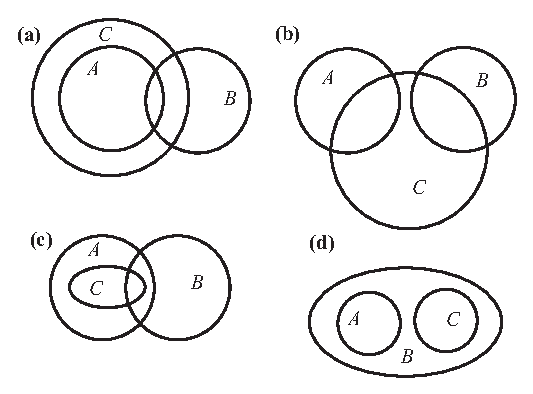
\includegraphics{xfig-exer12-41.eps}
\end{center}
\end{figure}


\item Using the standard setup for Venn diagrams with 3 sets,
\begin{enumerate}
\item $A \cap B$ corresponds to regions 2, 5.

\item $A \cap C$ corrresponds to regions 4, 5.

\item $(A \cap B) \cup (A \cap C)$ corresponds to regions 2, 4, 5.

\item $B \cup C$ corresponds to regions 2, 3, 4, 5, 6, 7.

\item $A \cap (B \cup C)$ corresponds to regions 2, 4, 5.

\item $(A \cap B) - C$ corresponds to region 2.
\end{enumerate}


\item \begin{enumerate}
\item Assume that $n$ is the sum of four consecutive integers.  So there exists an integer $k$ such that $n = (k - 1) + k + (k + 1) + (k + 2)$.  We then see that $n = 4k + 2$ and hence, 
$n \equiv 2 \pmod 4$.  Now assume that $n \equiv 2 \pmod 4$.  So there exists an integer $m$ such that $n = 4m + 2$.  We then see that $n = (m - 1) + m + (m + 1) + (m + 2)$ and hence, 
$n$ is the sum of four consecutive integers.

\item The set of all integers that are the sum of four consecutive integers is 
$\left\{ n \in \Z \mid n \equiv 2 \pmod 4 \right\}$.

\item The set of all natural numbers that are the sum of four consecutive integers is 
$\{10, 14, 18, 22, \ldots \, \}$.

\item Assume that $n$ is the sum of eight consecutive integers.  So there exists an integer $k$ such that
\[
n = (k - 3) + (k - 2) + (k - 1) + k + (k + 1) + (k + 2) + (k + 3) + (k + 4).
\]
We then see that $n = 8k + 4$ and hence, $n \equiv 4 \pmod 8$.  Now assume that 
$n \equiv 4 \pmod 8$.  So there exists an integer $m$ such that $n = 8m + 4$.  We then see that 
\[
n = (m - 3) + (m - 2) + (m - 1) + m + (m + 1) + (m + 2) + (m + 3) + (m + 4) 
\]
and hence, $n$ is the sum of eight consecutive integers.

\item The set of all integers that are the sum of eight consecutive integers is 
$\left\{ n \in \Z \mid n \equiv 4 \pmod 8 \right\}$.

\item The set of all natural numbers that are the sum of eight consecutive integers is 
$\{36, 44, 52, 60, \ldots \, \}$.
\end{enumerate}


\item This statement is false.  For a counterexample, we can use $U = \Z$ and let $A$ be the set of all odd integers and let $B$ be the set of all even integers.  In this case, 
$A \not\subseteq B$, $A \ne B$, and $B \not\subseteq A$.
\end{enumerate}




\subsection*{Explorations and Activities}
\setcounter{oldenumi}{\theenumi}
\begin{enumerate} \setcounter{enumi}{\theoldenumi}
\item \begin{enumerate}
\item The interval $\left( {a, b} \right)$  is a proper subset of   $\left( {a, b} \right]$ since 
$ b \in \left( a, b \right]$ and $b \notin \left( a, b \right)$.

\item The interval $\left[ a, b \right]$ is not a subset of $\left( a, + \infty \right)$ since 
$a \in \left[ a, b \right]$ and $a \notin \left( a + \infty \right)$.

\item $\left[ -3, 7 \right] \cap \left( 5, 9 \right] = \left( 5, 7 \right]$

\item $\left\{ {x \in \mathbb{R}} \mid \left| x \right| \leq 0.01 \right\} = \left[ -0.01, 0.01 \right]$

\item $\left\{  x \in \mathbb{R} \mid \left| x \right| > 2 \right\} = \left( { - \infty , 2} \right) \cup \left( {2, \infty } \right)$
\end{enumerate}


\item \begin{enumerate}
\item $[2, 5] \cap [-1, +\infty) = [2, 5]$ and $[2, 5] \cup [-1, +\infty] = [-1, +\infty)$

\item $[2, 5] \cap [3.4, +\infty) = [3.4, 5]$ and $[2, 5] \cup [3.4, +\infty) = [2, +\infty)$

\item $[2, 5] \cap [7, +\infty) = \emptyset$ and $[2, 5] \cup [7, +\infty)$ cannot be expressed as a single interval.

\item If $c \leq a$, then $[a, b] \cap [c, +\infty) = [a, b]$. If $a < c < b$, then 
$[a, b] \cap [c, +\infty) = [c, b]$.  If $c = b$, then $[a, b] \cap [c, +\infty) = {b}$.  If 
$b < c$, then $[a, b] \cap [c, +\infty) = \emptyset$.

\item If $c \leq a$, then $[a, b] \cup [c, +\infty) = [c, +\infty)$. If $a < c \leq b$, then 
$[a, b] \cup [c, +\infty) = [a, +\infty)$.  If $b < c$, then $[a, b] \cup [c, +\infty)$ cannot be expressed as a single interval.
\end{enumerate}



\item \setcounter{equation}{0}
\noindent
\textbf{Theorem~\ref{T:powerset}}.  Let  $n$  be a nonnegative integer and let  $A$  be a subset of some universal set.  If  $A$  is a finite set with  $n$  elements, then  $A$  has  $2^n $  subsets.  That is,  if  $\left| A \right| = n$, then  $\left| {\mathcal{P}\left( A \right)} \right| = 2^n $.

\vskip6pt
\noindent
For each nonnegative integer  $n$, let  $P\left( n \right)$ be, if  $A$  is a finite set with  
$n$  elements, then  $A$  has  $2^n $  subsets.

\begin{enumerate}
\item The statement  $P\left( 0 \right)$ is true since the empty set has  $2^0  = 1$ subset. 

\item The statement  $P\left( 1 \right)$ is true since a set with one element has  $2^1  = 2$ subsets.

The statement  $P\left( 2 \right)$ is true since a set with two elements has  $2^2  = 4$
 subsets. (The subsets of  $\left\{ {a, b} \right\}$ are  
$\emptyset$ , $\left\{ a \right\}, \left\{ b \right\}$, $\left\{ {a, b} \right\}$.)

\item Now assume that  $k$  is a nonnegative integer and assume that  $P\left( k \right)$ is true.  That is, assume that if a set has  $k$  elements, then that set has  $2^k $ subsets. 

Let  $A$  be a subset of the universal set with  $\left| A \right| = k + 1$, and let  $x \in A$.  Then, the set  $B = A - \left\{ x \right\}$  has  $k$  elements.  Since  $P\left( k \right)$
 is true, the set  $B$  has  $2^k $ subsets.

Now, by Lemma~\ref{L:inductivestepforsubsets},  each subset of  $A$  is a subset of  $B$  or a set of the form  
$C = B \cup \left\{ x \right\}$ where  $C$  is a subset of  $B$.  So, if  $B$  has  $2^k $
 subsets, then the number of subsets of  $A$ is equal to
\[
2^k  + 2^k  = 2 \cdot 2^k  = 2^{k + 1} .
\]
This proves that if  $P\left( k \right)$ is true, then  $P\left( {k + 1} \right)$ is true.  Hence, by the Second Principle of Mathematical Induction,  $P\left( n \right)$ is true for each nonnegative integer  $n$.
\end{enumerate}

\end{enumerate}





\hbreak
\endinput

\item 
\begin{enumerate}
\item 
\begin{figure}[h]
\includegraphics[2.5cm,1.8cm]{xfigexer-41-9a.bmp}
\end{figure}

\item 
\begin{figure}[h]
\includegraphics[2.5cm,1.8cm]{xfigexer-41-9b.bmp}
\end{figure}

\section*{Section \ref{S:provingset} Proving Set Relationships}

\begin{enumerate}
%\item \begin{enumerate}
%\item If $x \in A$, then there exists an integer $k$ such that $x = 9k$.  This means that 
%$x = 3 \left( 3k \right)$ and since $3k \in \mathbb{Z}$, we see that $x \in B$.
%
%\item The set $B$ is not a subset of $A$ since there exist elements (such as 3 and 6) that are in 
%$B$ but not in $A$.
%\end{enumerate}

\item \begin{enumerate}
\item The set  $A$  is  a subset of  $B$.  If  $x \in A$, then  
$ - 2 < x < 2$.  Hence,  $x < 2$ and we conclude that  $x \in B$.

\item The set  $B$  is not a subset of  $A$ since there exist real numbers that are in  $B$  but not in  $A$.  For example, $-4$ and $-3$ are in $B$ but not in $A$.
\end{enumerate}


\item 
\begin{enumerate}\setcounter{enumii}{1}
\item Assume that $A \subseteq B$ and that $B \subseteq C$, and let $x \in A$.  Then, $x \in B$ since $A$ is a subset of $B$, and since $B$ is a subset of $C$, this implies that $x \in C$.  Hence,$A \subseteq C$.
\end{enumerate}


\item \begin{enumerate} \setcounter{enumii}{1}
\item To prove that $A \subseteq B$, let $x \in A$.  Then, $x \equiv 7 \pmod 8$ and so, 
$8 \mid \left( x - 7 \right)$.  This means that there exists an integer $m$ such that
\[
x - 7 = 8m.
\]
By adding 4 to both sides of this equation, we see that $x - 3 = 8m + 4$, or 
$x - 3 = 4 \left( 2m + 1 \right)$.  From this, we conclude that $4 \mid \left( x - 3 \right)$ and that $x \equiv 3 \pmod 4$.  Hence, $x \in B$.

\item $B \not \subseteq A$.  For example, $3 \in B$ and $3 \notin A$.
\end{enumerate}


\item \begin{enumerate} \setcounter{enumii}{1}
\item To prove that $C \subseteq D$, let $x \in C$.  Then, $x \equiv 7 \pmod 9$ and so, 
$9 \mid \left( x - 7 \right)$.  This means that there exists an integer $m$ such that
\[
x - 7 = 9m.
\]
By adding 6 to both sides of this equation, we see that $x - 1 = 9m + 6$, or 
$x - 1 = 3 \left( 3m + 2 \right)$.  From this, we conclude that $3 \mid \left( x - 1 \right)$ and that $x \equiv 1 \pmod 3$.  Hence, $x \in D$.

\item $D \not \subseteq C$.  For example, $4 \in D$ and $4 \notin C$.
\end{enumerate}


\item \begin{enumerate}
\item $A = \left\{ x \in \Z \mid \mod{x}{2}{3} \right\} = B = \left\{ y \in \Z \mid 6 \text{ divides } (2y - 4) \right\}$.

\noindent
Notice that if $x \in A$, then there exists an integer $m$ such that $x - 2 = 3m$.  We can use this equation to see that $2x - 4 = 6m$ and so 6 divides $(2x - 4$.  Therefore, $x \in B$.

\noindent
Conversely, if $y \in B$, then there exists an integer $m$ such that $2y - 4 = 6m$.  Hence, $y - 2 = 3m$, which implies that $\mod{y}{2}{3}$ and $y \in A$.

\item For $A = \left\{ x \in \Z \mid \mod{x}{3}{4} \right\}$ and 
$B = \left\{ y \in \Z \mid 3 \text{ divides } (y - 2) \right\}$, none of the relations are true.  We can see that $A \not \subseteq B$ since $3 \in A$ and $3 \notin B$.  We can also see that $B \not \subseteq A$ since $2 \in B$ and $2 \notin A$.  In addition, the two sets are not disjoint since $11 \in (A \cap B)$.

\item If $A = \left\{ x \in \Z \mid \mod{x}{1}{5} \right\}$ and 
$B = \left\{ y \in \Z \mid \mod{y}{7}{10} \right\}$, then $A \cap B = \emptyset$.

\noindent
Use a proof by contradiction and assume that $A \cap B \ne \emptyset$.  So there exists an $x$ in $A \cap B$.  We can then conclude that there exist integers $m$ and $n$ such that $x - 1 = 5m$ and $x - y = 10n$.  So $x = 5m + 1$ and $x = 10n + 7$.  We then see that
\begin{align*}
5m + 1 &= 10n + 7 \\
5(m - 2n) &= 6
\end{align*}
The last equation implies that 5 divides 6, and this is a contradiction.
\end{enumerate}


\item \begin{enumerate}
\item We will use the fact that $x^2 - 3x - 10 = (x + 2)(x - 5)$.  Let 
$a \in \left\{x \in \R \mid x^2 - 3x - 10 < 0 \right\}$.  We can then conclude that 
\[
(a + 2)(a - 5) < 0
\]
and this means that either $a + 2 < 0$ and $a - 5 > 0$ or 
$a + 2 > 0$ and $a - 5 < 0$.  However, in the first case, $a < -2$ and $a > 5$ and this is  impossible.  Therefore, $a > -2$ and $a < 5$, which means that $-2 < a < 5$ and 
$a \in \left\{ x \in \R \mid -2 < x < 5 \right\}$.  

We now assume that 
$b \in \left\{ x \in \R \mid -2 < x < 5 \right\}$.  Then $-2 < b < 5$.  This implies that 
$b + 2 > 0$ and $b - 5 < 0$ and, hence, $(b + 2)(b - 5) < 0$ or $b^2 - 3b - 10 < 0$.  Therefore, 
$b \in \left\{x \in \R \mid x^2 - 3x - 10 < 0 \right\}$ and we have proved that 
\[
\left\{x \in \R \mid x^2 - 3x - 10 < 0 \right\} = \left\{ x \in \R \mid -2 < x < 5 \right\}
\]
since we have proved that each set is a subset of the other set.

\item We will use the fact that $x^2 - 5x + 6 = (x - 2)(x - 3)$.  Let 
$a \in \left\{x \in \R \mid x^2 - 5x + 6 < 0 \right\}$.  We can then conclude that 
\[
(a - 2)(a - 3) < 0
\]
and this means that either $a - 2 < 0$ and $a - 3 > 0$ or 
$a - 2 > 0$ and $a - 3 < 0$.  However, in the first case, $a < 2$ and $a > 3$ and this is  impossible.  Therefore, $a > 2$ and $a < 3$, which means that $2 < a < 3$ and 
$a \in \left\{ x \in \R \mid 2 < x < 3 \right\}$.  

We now assume that 
$b \in \left\{ x \in \R \mid 2 < x < 3 \right\}$.  Then $2 < b < 3$.  This implies that 
$b - 2 > 0$ and $b - 3 < 0$ and, hence, $(b - 2)(b - 3) < 0$ or $b^2 - 5b + 6 < 0$.  Therefore, 
$b \in \left\{x \in \R \mid x^2 - 5x + 6 < 0 \right\}$ and we have proved that 
\[
\left\{x \in \R \mid x^2 - 5x + 6 < 0 \right\} = \left\{ x \in \R \mid 2 < x < 3 \right\}
\]
since we have proved that each set is a subset of the other set.

\item Let $a \in \left\{x \in \R \mid x^2 \geq 4 \right\}$.  Then $a^2 - 4 \geq 0$ or 
$(a + 2)(a - 2) \geq 0$.  This means that $a + 2 \leq 0$ and $a - 2 \leq 0$ or $a + 2 \geq 0$ and 
$a - 2 \geq 0$.  In the first case, $a \leq -2$ and in the second case, $a \geq 2$. This proves that $a \leq -2$ or $a \geq 2$ and, hence, 
$a \in \left\{x \in \R \mid x \leq -2 \right\} \cup \left\{x \in \R \mid x \geq 2 \right\}$.

Now let 
$b \in \left\{x \in \R \mid x \leq -2 \right\} \cup \left\{x \in \R \mid x \geq 2 \right\}$.  Then $b \leq -2$ or $b \geq 2$.  In the first case, $b + 2 \leq 0$ and $b - 2 \leq 0$ and, hence, 
$(b + 2)(b - 2) \geq 0$, which means $b^2 \geq 4$.  In the second case, $b + 2 \geq 0$ and 
$b - 2 \geq 0$ and, hence, $(b + 2)(b - 2) \geq 0$, which means $b^2 \geq 4$.  In both cases, 
$b \in \left\{x \in \R \mid x^2 \geq 4 \right\}$.  So we have proved that
\[
\left\{x \in \R \mid x^2 \geq 4 \right\} = \left\{x \in \R \mid x \leq -2 \right\} \cup \left\{x \in \R \mid x \geq 2 \right\}
\]
since we have proved that each set is a subset of the other set.
\end{enumerate}


\item \begin{enumerate}
\item Let $x \in A \cap B$.  Then, $x \in A$ and $x \in B$.  This proves that 
$A \cap B \subseteq A$.

\item Let $x \in A$.  Then, the statement ``$x \in A$ or $x \in B$'' is true.  Hence, 
$A \subseteq A \cup B$.

\item By Part~(a), $A \cap A \subseteq A$.  Now, let $x \in A$.  Then, the statement 
``$x \in A$ and $x \in A$'' is true.  Hence, $A \subseteq A \cap A$ and so, $A \cap A = A$.

\item By Part~(b), $A \subseteq A \cup A$.  Now, let $x \in A \cup A$.  Then, the statement 
``$x \in A$ or $x \in A$'' is true.  Hence, $x \in A$, and therefore, $A \cup A \subseteq A$ and so, $A \cup A = A$.

\item We know that $\emptyset \subseteq A \cap \emptyset$.  By Part~(a), 
$A \cap \emptyset \subseteq \emptyset$.  Therefore, $A \cap \emptyset = \emptyset$.

\item By Part~(b), $A \subseteq A \cup \emptyset$.  So, let $x \in A \cup \emptyset$.  Then, 
$x \in A$ or $x \in \emptyset$.  Since $x$ cannot be in the empty set, we conclude that $x \in A$.  Therefore, $A \cup \emptyset \subseteq A$ and so, $A \cup \emptyset = A$.
\end{enumerate}


\item We still need to prove that if $B^c \subseteq A^c$, then $A \subseteq B$.  We will prove the contrapositive.  So we assume there exists an element $y$ in $A$ such that $y \notin B$.  Then $y \notin A^c$ and $y \in B^c$.  This means that $B^c \not\subseteq A^c$ and this proves the contrapositive.


%\item The statement is true.  Prove the contrapositive, which is ``If $A \not\subseteq B$, then 
%$A \cap B^c \ne \emptyset$.``  So, we assume $A \not\subseteq B$.  This means that there exists an element $x$ that is in $A$ and not in $B$.  From this, we conclude that $x \in A$ and $x \in B^c$.  Consequently, $A \cap B^c \ne \emptyset$.

\item The statement is true.  To prove it, use a proof by contradiction.  So, we assume that 
$A \cap B$ and $A - B$ are not disjoint.  This means that there exists an element $x$ such that 
$x \in A \cap B$ and $x \in A - B$.  Since $x \in A \cap B$, we conclude that $x \in B$, and since $x \in A - B$, we conclude that $x \notin B$.  This is a contradiction.  Therefore, 
$A \cap B$ and $A - B$ are disjoint.


\item Prove the contrapositive.  So assume that $A$ and $B$ are subsets of some universal set $U$ and that $A \not \subseteq B$.  Then, there exists an element $x \in A$ such that $x \notin B$.  We can then conclude that $x in A$ and $x \in B^c$.  Hence, $x \in A \cap B^c$ and $A \cap B^c \ne \emptyset$.  This proves the contrapositive.




\item \begin{enumerate}
\item This statement is false.  With $U = \N$, a counterexample is $A = \{1\}$, 
$B = \{ 1, 2, 3 \}$, $C = \{ 2 \}$, and $D = \{ 2, 3 \}$.  An appropriate Venn diagram could also be used to provide a counterexample.

\item This statement is true.  Use a proof by contradiction.  So assume that $A \subseteq B$, $C \subseteq D$, and 
$A \cap C \ne \emptyset$.  Since $A \cap C \ne \emptyset$, let $x \in A \cap C$.  Since $A \subseteq B$, $x \in B$, and since $C \subseteq D$, $x \in D$. This means that $B \cap D \ne \emptyset$, which contradicts the assumption that $B$ and $D$ are disjoint.
\end{enumerate}


\item \begin{enumerate}
\item Assume that $A$ is a subset of $B$, and let $x \in A \cap C$.  Then, $x \in A$ and 
$x \in C$.  Since $x \in A$ and $A \subseteq B$, we know that $x \in B$.  Thus, $x \in B$ and 
$x \in C$, and hence $x \in B \cap C$.  Therefore, if $x \in A \cap C$, then $x \in B \cap C$ and hence, $A \cap C \subseteq B \cap C$.

\item Assume that $A$ is a subset of $B$, and let $x \in A \cup C$.  Then, $x \in A$ or 
$x \in C$.  In the case where $x \in A$, we see that $x \in B$ since $A \subseteq B$.  So, in this case, $x \in B \cup C$.  In the case where $x \in C$, we also conclude that $x \in B \cup C$. Therefore, if $x \in A \cup C$, then $x \in B \cup C$ and hence, $A \cup C \subseteq B \cup C$.
\end {enumerate}


\item \begin{enumerate}
\item The statement is false.  A counterexample is $A = \left\{ 1, 2 \right\}$, 
$B = \left\{ 2, 3 \right\}$, and $C = \left\{ 2 \right\}$.  Then, $A \cap C = \left\{ 2 \right\}$ and $B \cap C = \left\{ 2 \right\}$, but $A \not\subseteq B$.

\item The statement is false.  A counterexample is $A = \left\{ 1, 2 \right\}$, 
$B = \left\{ 1 \right\}$, and $C = \left\{ 2, 3 \right\}$.  Then, 
$A \cup C = \left\{ 1, 2, 3 \right\}$ and $B \cup C = \left\{ 1, 2, 3 \right\}$, but 
$A \not\subseteq B$.

\item This statement is false.  The counterexample for Part~(b) is also a counterexample for this statement.

\item This statement is false.  The counterexample for Part~(a) is also a counterexample for this statement.
%A counterexample is $A = \{1, 2, 3\}$, $B = \{2 \}$, and 
%$C = \{1, 2, 3 \}$.  Then $A \cap C = \{1, 2, 3 \}$, $B \cup C = \{1, 2, 3 \}$, and $A \ne B$.

\item This statement is true.  To prove that $A \subseteq B$, let $x \in A$.  Then 
$x \in A \cup C$ and since $A \cup C = B \cup C$, $x \in B \cup C$.  So $x \in B$ or $x \in C$.  If $x \in C$, then $x \in A \cap C$ and since $A \cap C = B \cap C$, $x \in B \cap C$.  This means that $x \in B$.  So $x$ must be in $B$ and this proves that $A \subseteq B$.  The proof that $B \subseteq A$ is similar.
\end{enumerate}


\item To prove $B \subseteq C$, let $x \in B$.  Use two cases: $x \in A$ or $x \notin A$.  If $x \in A$, then $x \in A \cap B$.  Since $A \cap B = A \cap C$, $x \in A \cap C$ and therefore, $x \in C$.  If $x \notin A$, then $x \in A^c$ and $x \in A^c \cap B$.  Since 
$A^c \cap B = A^c \cap C$, $x \in A^c \cap C$ and therefore, $x \in C$.  In both cases, $x \in C$ and this proves that $B \subseteq C$.  Now use a similar proof to prove that $C \subseteq B$.


\item \begin{enumerate}
\item If $A \subseteq B$, then $A \cap B^c = \emptyset$ was proved in Proposition~4.14.  For the converse, prove the contrapositive, which states that if $A \cap B^c \ne \emptyset$, then 
$A \not\subseteq B$. Since $A \cap B^c \ne \emptyset$, there exists an element 
$x \in A \cap B^c$.  This means that $x \in A$ and $x \notin B$, which implies that 
$A \not\subseteq B$.

\item First, assume $A \subseteq B$.  We know that $B \subseteq A \cup B$, so let 
$x \in A \cup B$.  Then $x \in A$ or $x \in B$. However, if $x \in A$, then since 
$A \subseteq B$.  So in both cases, $x \in B$ and hence, $A \cup B \subseteq B$.  This proves that if $A \subseteq B$, then $A \cup B = B$.

Now assume that $A \cup B = B$ and let $x \in A$. Then $x \in A \cup B$ and since 
$A \cup B = B$, we see that $x \in B$.  Hence, $A \subseteq B$.

\item First, assume $A \subseteq B$.  We know that $A \cap B \subseteq A$, so let 
$x \in A$.  Then $x \in B$ and, hence, $x \in A \cap B$. This proves that if $A \subseteq B$, then $A \cap B = A$.

Now assume that $A \cap B = A$ and let $x \in A$. Then since $A \cap B = A$, $x \in A \cap B$, and we see that $x \in B$.  Therefore, $A \subseteq B$.

\item The following conditional statement is false:
\begin{list}{}
\item If $A \subseteq B \cup C$, then $A \subseteq B$ or $A \subseteq C$.
\end{list}
A counterexample is $A = \{1, 2, 3 \}$, $B = \{1, 2 \}$, and $C = \{2, 3 \}$.

The following conditional statement is true:
\begin{list}{}
\item If $A \subseteq B $ or $A \subseteq C$, then $A \subseteq B \cup C$.
\end{list}
\item Assume $A \subseteq B$ and $A \subseteq C$ and let $x \in A$.  Then $x \in B$ and $x \in C$ and hence, $x \in B \cap C$, and we conclude that $A \subseteq B \cap C$.

Now assume $A \subseteq B \cap C$.  Since $B \cap C \subseteq B$ and $B \cap C \subseteq C$, we can conclude that $A \subseteq B$ and $A \subseteq C$.
\end{enumerate}


\item \begin{enumerate}
\item If $a \in T$, then $a \in S \cup T$ and hence, $a \in X \cup Y$.

\item If $a \in T$, then $a \notin S$.

\item If $a \in T$, then $a \in X \cup Y$, which means that $a \in X$ or $a \in Y$.  However, if $a \in X$, then since $X \subseteq S$, we know that $a$ must be in $S$.  However, we have shown in Part~(b) that $a \notin S$.  Therefore, $a \notin X$ and hence, $a$ must be in $Y$.  
Consequently, $T \subseteq Y$.
\end{enumerate}



%\item The statement is true.  Assume that $a$ and $b$ are integers with $a \ne 0$ and that $a \mid b$.  Now, let 
%$x \in \mathbb{Z}$ with $x \ne 0$.  We will prove that $ax \mid bx$.  Since $a \mid b$, there exists an integer $k$ such that $b = ak$.  Multiplying both sides of this equation by $x$ gives 
%$bx = \left( ax \right) k$.  This proves that $ax \mid bx$.
%
%\item \begin{enumerate}
%\item One way is to prove that a certain even natural number greater than 2 cannot be written as the sum of two prime numbers.
%
%\item  Prove the contrapositive, which is:
%\begin{list}{}
%\item  If Goldbach's conjecture is true, then every odd integer greater than 5 is the sum of three prime numbers.
%\end{list}
%To prove this, let $n$ be an odd integer that is greater than 5.  Then, $n-3$ is an even integer that is greater than 2.  If Goldbach's Conjecture is true, then there exist prime numbers $p$ and $q$ such that $n - 3 = p + q$.  Then,
%\[
%n = p + q + 3,
%\]
%and we see that $n$ is the sum of three prime numbers.
%\end{enumerate}
\end{enumerate}




\subsection*{Evaluations of Proofs}
\setcounter{oldenumi}{\theenumi}
\begin{enumerate} \setcounter{enumi}{\theoldenumi}
\item \begin{enumerate}
\item This proposition is false.  Following is a counterexample.

\noindent
Let $U = \Z$ and let $A = \{1 \}$, $B = \{2 \}$, and $C = \{1, 3\}$.  In this example, 
$A \not \subseteq B$ and $B \notsubseteq C$ and $A \subseteq C$.

\vskip6pt
\noindent
A problem with the proposed proof is that $x$ was used for two different elements.  We can only conclude that there exists an element in $A$ that is not in $B$ and that there exists an element in $B$ that is not in $C$.  There is no guarantee that these two elements must be the same.  So if we use $x$ for the element that is in $A$ but not in $B$, we must use a different letter for the element that is in $B$ but not in $C$.

\item This proposition is false.  Following is a counterexample.

\noindent
Let $U = \Z$ and let $A = \{1 \}$, $B = \{1, 2 \}$, and $C = \{1, 3\}$.  In this example, 
$A \cap B = \{1 \}$, $A \cap C = \{1 \}$ and so, $A \cap B = A \cap C$.  However, $B \ne C$.

\noindent
There is a problem in the second paragraph in the proposed proof.  We can get to the conclusion that $x \notin A \cap C$.  However, care was not taken at this point.  From here, it is only possible to conclude that $x \notin A$ or $x \notin C$.  The fact that $x \notin A$ does not allow us to conclude that $x$ must be in $C$.


\item This proposition is false.  Following is a counterexample.

\noindent
Let $U = \Z$ and let $A = \{1 \}$, $B = \{2, 3 \}$, and $C = \{1, 2, 3\}$.  In this example, 
$A \not \subseteq B$, $B \subseteq C$, and $A \subseteq C$.

\vskip6pt
\noindent
In the proposed proof, it is legitimate to conclude that there exists an element $x$ such that 
$x \in A$ and $x \notin B$.  However, the assumption that $B \subseteq C$ allows us to conclude that if $y \in B$, then $y \in C$ or that if $y \notin C$, then $y \notin B$.  We cannot use this assumption to conclude that $x \notin C$ because $x \notin B$.
\end{enumerate}
\end{enumerate}



\subsection*{Explorations and Activities}
\setcounter{oldenumi}{\theenumi}
\begin{enumerate} \setcounter{enumi}{\theoldenumi}
\item \begin{enumerate}
\item Let  $a = 20$, $b = 12$, and  $d = 4$.  In this case,  $d \mid a$ and $d \mid b$. 
\begin{center}
\begin{tabular}[t]{| c | c | c | c |} \hline
$x$  &  $y$  &  $ax + by$  &	Does  $d$  divide  $ax + by$? \\ \hline
1  &	1  &	32  &	Yes \\ \hline
1  &	$-1$ &	8   &	Yes \\ \hline
2  &	2  &	64  &	Yes \\ \hline
2  &	$-3$ &	4   &	Yes \\ \hline
$-2$ &	3  &	$-4$  &	Yes \\ \hline
$-2$ &	$-5$ &	$-100$ & Yes \\ \hline
\end{tabular}
\end{center}

\item Let  $a = 21$, $b =  - 6$, and  $d = 3$. In this case,  $d \mid a$ and $d \mid b$.
\begin{center}
\begin{tabular}[t]{| c | c | c | c |} \hline
$x$  &  $y$  &  $ax + by$  &	Does  $d$  divide  $ax + by$? \\ \hline
1  &	1  &	15  &	Yes \\ \hline
1  &	$-1$ &	27  &	Yes \\ \hline
2  &	2  &	30  &	Yes \\ \hline
2  &	$-3$ &	60   &	Yes \\ \hline
$-2$ &	3  &	$-60$  &	Yes \\ \hline
$-2$ &	$-5$ &	$-72$ & Yes \\ \hline
\end{tabular}
\end{center}

\item \textbf{Proposition~\ref{P:divlinearcomb}}.  Let $a$, $b$, and  $d$  be integers.  If  $d$  divides  $a$  and  $d$  divides  $b$, then for all integers  $x$  and  $y$,  $d$  divides  $ax + by$.

\begin{myproof}
Let $a$, $b$, and  $d$  be integers, and assume that $d$  divides  $a$  and  $d$  divides  $b$.  We will prove that for all integers  $x$  and  $y$,  $d$  divides  $ax + by$.

So, let  $x \in \mathbb{Z}$ and let  $y \in Z$.  Since  $d$  divides  $a$ and $d$ divides $b$, there exist an integers  $m$ and $n$  such that
\[
a = md \qquad \text{ and } \qquad b = nd.
\]
We substitute the expressions for  $a$  and  $b$  given in these two equations into  $ax + by$.  This gives
\[
\begin{aligned}
  ax + by &= \left( {md} \right)x + \left( {nd} \right)y \\ 
          &= d\left( {mx + ny} \right). \\ 
\end{aligned} 
\]
By the closure properties of the integers,  $mx + ny$ is an integer, and hence we may conclude that  $d$  divides  $ax + by$.  Since  $x$  and  $y$  were chosen as arbitrary integers, we have proven that if  $d$  divides  $a$  and  $d$  divides  $b$, then for all integers  $x$  and  $y$,  $d$  divides  $ax + by$.
\end{myproof}


\end{enumerate}
\end{enumerate}

\hbreak




\endinput

\section*{Section \ref{S:setproperties} Properties of Set Operations}

\begin{enumerate}
\item \begin{enumerate}
\item Let  $x \in \left( A^c \right)^c$.  Then  $x \notin A^c$, and if $x \notin A^c$, then 
$x \in A$.  Therefore, $\left( A^c \right)^c \subseteq A$.  Now let $y \in A$.  Then, 
$y \notin A^c$ and hence, $y \in \left( A^c \right)^c$.  Therefore, 
$A \subseteq \left( A^c \right)^c$.

\item If $x \in A - \emptyset$, then $x \in A$ and $x \notin \emptyset$.  Therefore, $x \in A$ and hence, $A - \emptyset \subseteq A$.  Also, if $y \in A$, then since $y \notin \emptyset$, 
$y \in A - \emptyset$.  Therefore, $A \subseteq A - \emptyset$.

\item  First, $\emptyset^c \subseteq U$.  Also, if $x \in U$, then $x \notin \emptyset$ and hence, 
$x \in \emptyset^c$.  Therefore, $U \subseteq \emptyset^c$.

\item By Part~(c), $\emptyset^c = U$. Hence, by $\left( \emptyset^c \right)^c = U^c$.  Therefore, by Part~(a), $\emptyset = U^c$.
\end{enumerate}



\item We will first prove that $A \cap \left( B \cup C \right) \subseteq \left( A \cap B \right) 
\cup \left( A \cap C \right)$.  Let $x \in A \cap \left( B \cup C \right)$.  Then $x \in A$ and 
$x \in B \cup C$.  So we will use two cases: \\
(1) $x \in B$; (2) $x \in C$.

In Case~(1), $x \in A \cap B$ and hence, $x \in \left( A \cap B \right) \cup \left( A \cap C \right)$.  In Case~(2), $x \in  A \cap C$ and hence, $x \in \left( A \cap B \right) \cup \left( A \cap C \right)$.  This proves that $A \cap \left( B \cup C \right) \subseteq \left( A \cap B \right) 
\cup \left( A \cap C \right)$.

We now prove that $\left( A \cap B \right) \cup \left( A \cap C \right) \subseteq 
A \cap \left( B \cup C \right)$.  
Let $x \in \left( A \cap B \right) \cup \left( A \cap C \right)$.  Then, $x \in A \cap B$ or 
$x \in A \cap C$.  If $x \in A \cap B$, then $x \in A$ and $x \in B$.  Therefore, $x \in A$ and 
$x \in B \cup C$.  So, we may conclude that $x \in A \cap \left( B \cup C \right)$.  In a similar manner, we can prove that if $x \in A \cap C$, then $x \in A \cap \left( B \cup C \right)$.  This proves that $\left( A \cap B \right) \cup \left( A \cap C \right) \subseteq 
A \cap \left( B \cup C \right)$, and hence that $A \cap \left( B \cup C \right) = \left( A \cap B \right) \cup \left( A \cap C \right)$. 



\item Let $x \in \left( A \cap B \right)^c$.  Then, $x \notin A \cap B$.  This means that 
$x \notin A$ or $x \notin B$ and hence that $x \in A^c$ or $x \in B^c$.  This proves that 
$\left( A \cap B \right)^c \subseteq A^c \cup B^c$.

Now, let $x \in A^c \cup B^c$.  Then, $x \in A^c$ or $x \in B^c$.  This means that $x \notin A$ or 
$x \notin B$.  In both of these cases, we may conclude that $x \notin A \cap B$ and hence that 
$x \in \left( A \cap B \right)^c$.  Therefore, 
$A^c \cup B^c \subseteq \left( A \cap B \right)^c$.



\item \begin{enumerate}
\item $A - \left( {B \cup C} \right) = \left( {A - B} \right) \cap \left( {A - C} \right)$.

\item Let $x \in A - \left( {B \cup C} \right)$.  Then, $x \in A$ and $x \notin \left( B \cup C 
\right)$.  Hence, we may conclude that $x \notin B$ and $x \notin C$.  So,
\begin{list}{}
\item $x \in A$ and $x \notin B$.  Therefore, $x \in A - B$.
\item $x \in A$ and $x \notin C$.  Therefore, $x \in A - C$.
\end{list}
Thus, $x \in \left( A - B \right) \cap \left( A - C \right)$ and this proves that 
$A - \left( {B \cup C} \right) \subseteq \left( {A - B} \right) \cap \left( {A - C} \right)$.

Now, let $x \in \left( {A - B} \right) \cap \left( {A - C} \right)$.  Then, $x \in A - B$ and 
$x \in A - C$.  Hence, $x \in A$, $x \notin B$, and $x \notin C$.  This means that 
$x \in A$ and $x \notin B \cup C$.  Hence, $x \in A - \left( B \cup C \right)$, and this proves that $\left( {A - B} \right) \cap \left( {A - C} \right) \subseteq  A - \left( B \cup C \right)$.

\item 
\[
\begin{aligned}
\left( A - B \right) \cap \left( A - C \right) &= \left( A \cap B^c \right) \cap \left( A \cap C^c \right) \\
  &= \left( A \cap A \right) \cap \left( B^c \cap C^c \right) \\
  &= A \cap \left( B \cup C \right)^c \\
  &= A - \left( B \cup C \right).
\end{aligned}
\]
\end{enumerate}



\item \begin{enumerate}
\item $A - \left( {B \cap C} \right) = \left( {A - B} \right) \cup \left( {A - C} \right)$.

\item Let $x \in A - \left( {B \cap C} \right)$.  Then, $x \in A$ and 
$x \notin \left( B \cap C \right)$.  So, $x \notin B$ or $x \notin C$.  This means that 
$x \in A$ and $x \notin B$ or that $x \in A$ and $x \notin C$.  Hence, 
$x \in \left( A - B \right) \cup \left( A - C \right)$.  This proves that 
$A - \left( {B \cap C} \right) \subseteq \left( A - B \right) \cup \left( A - C \right)$.

Now let $x \in \left( A - B \right) \cup \left( A - C \right)$.  Then, $x \in A - B$ or 
$x \in A - C$.  If $x \in A - B$, then $x \in A$ and $x \notin B$ and hence, 
$x \notin B \cap C$.  Therefore, $x \in A - \left( B \cap C \right)$.  Similary, if $x \in A - C$, then $x \in A - \left( B \cap C \right)$.  This proves that 
$\left( A - B \right) \cup \left( A - C \right) \subseteq A - \left( B \cap C \right)$.

\item 
\[
\begin{aligned}
A - \left( B \cap C \right) &= A \cap \left( B \cap C \right)^c \\
  &= A \cap \left( B^c \cup C^c \right) \\
  &= \left( A \cap B^c \right) \cup \left( A \cap C^c \right) \\
  &= \left( A - B \right) \cup \left( A - C \right). \\
\end{aligned}
\]
\end{enumerate}


\item \begin{enumerate}
\item \begin{align*}
(A - C) \cap (B - C) &= (A \cap C^c) \cap (B \cap C^c) \\
                     &= (A \cap B) \cap (C^c \cap C^c) \\
                     &= (A \cap B) \cap C^c \\
                     &= (A \cap B) - C.
\end{align*}

\item \begin{align*}
(A \cup B) - (A \cap B) &= (A \cup B) \cap (A \cap B)^c \\
                        &= (A \cup B) \cap (A^c \cup B^c) \\
               &= \left[ (A \cup B) \cap A^c \right] \cup \left[ (A \cup B) \cap B^c \right] \\
               &= \left[ (A \cap A^c) \cup (B \cap A^c) \right] \cup \left[ (A \cap B^c) \cup (B \cap B^c) \right] \\
               &= \left[ \emptyset \cup (B \cap A^c) \right] \cup \left[ (A \cap B^c) \cup \emptyset \right] \\
               &= (B \cap A^c) \cup (A \cap B^c) \\
               &= (B - A) \cup (A - B) \\
               &= (A - B) \cup (B - A).
\end{align*}
\end{enumerate}



\item \begin{enumerate}
\item The Venn diagrams should show that $\left( A - B \right) - C \subseteq A - \left( B - C \right)$.

\item Let $x \in \left( A - B \right) - C$.  Then, $x \in \left( A - B \right)$ and 
$x \notin C$.  Since $x \in \left( A - B \right)$, we conclude that $x \in A$ and $x \notin B$.  However,\linebreak
$x \notin B$ implies that $x \notin \left( B - C \right)$.  Therefore, 
$x \in A - \left( B - C \right)$ and $\left( A - B \right) - C \subseteq A - \left( B - C \right)$.
\end{enumerate}


\item \begin{enumerate}
\item The Venn diagrams should show that $A - (B - C) = (A - B) \cup \left( A - C^c \right)$.

\item Using the algebra of sets, we see that
\begin{align*}
A - (B - C) &= A -  \left(B \cap C^c \right)\\
            &= A \cap \left(B \cap C^c \right)^c \\
            &= A \cap \left( B^c \cup \left( C^c \right)^c \right) \\
            &= \left( A \cap B^c \right) \cup \left( A \cap \left( C \right)^c \right) \\
            &= (A - B) \cup \left( A - C^c \right)
\end{align*}

\end{enumerate}


\item \begin{enumerate}
\item If $x \in A \cap \left( B - A \right)$, then $x \in A$ and $x \in B - A$.  However, if 
$x \in B - A$, then $x \notin A$.  This contradicts the conclusion that $x \in A$.  Therefore, 
$A$ and $B - A$ are disjoint.

\item Let $x \in A \cup B$.  Then $x \in A$ or $x \in B$.  If $x \in A$, then 
$x \in A \cup \left( B - A \right)$.  If $x \in B$, then $x \in A$ or $x \notin A$.  In the first case, $x \in A \cup \left( B - A \right)$, and in the second case, $x \in B - A$ and so 
$x \in A \cup \left( B - A \right)$.  Thus, $A \cup B \subseteq A \cup \left( B - A \right)$

Now, since $B - A \subseteq B$, it can be seen that 
$A \cup \left( B - A \right) \subseteq A \cup B$.
\end{enumerate}



\item \begin{enumerate}
\item If $x \in A - B$ and $x \in A \cap B$, then $x \notin B$ and $x \in B$.  This is impossible.  Therefore, $A - B$ and $A \cap B$ are disjoint.

\item Since $A - B \subseteq A$ and $A \cap B \subseteq A$, it is seen that 
$\left( A - B \right) \cup \left( A \cap B \right) \subseteq A$.

Now, let $x \in A$.  Then $x \in B$ or $x \notin B$.  If $x \in B$, then $x \in A \cap B$.  If 
$x \notin B$, then $x \in A - B$.  In both cases, 
$x \in \left( A - B \right) \cup \left( A \cap B \right)$.  Therefore, 
$A \subseteq \left( A - B \right) \cup \left( A \cap B \right)$.
\end{enumerate}


\item \begin{enumerate}
\item \begin{align*}
A - (A \cap B^c) &= A \cap (A \cap B^c)^c \\
                 &= A \cap (A^c \cup B) \\
                 &= (A \cap A^c) \cup (A \cap B) \\
                 &= \emptyset \cup (A \cap B) \\
                 &= A \cap B.
\end{align*}

\item \begin{align*}
\left( A^c \cup B \right)^c \cap A &= \left( A \cap B^c \right) \cap A \\
                                   &= A \cap B^c \\
                                   &= A - B.
\end{align*}

\item \begin{align*}
(A \cup B) - A &= (A \cup B) \cap A^c \\
               &= (A \cap A^c) \cup (B \cap A^c) \\
               &= \emptyset \cup (B - A) \\
               &= B - A.
\end{align*}

\item \begin{align*}
(A \cup B) - B &= (A \cup B) \cap B^c  &  A - (A \cap B) &= A \cap (A \cap B)^c \\
               &= (A \cap B^c) \cup (B \cap B^c) &       &= A \cap (A^c \cup B^c)  \\
               &= (A - B) \cup \emptyset         &       &= (A \cap A^c) \cup (A \cap B^c) \\
               &= A - B.                         &       &= \emptyset \cup (A - B) \\
               &                                 &       &= A - B.
\end{align*}

\item \begin{align*}
(A \cup B) - (A \cap B) &= (A \cup B) \cap (A \cap B)^c \\
                        &= (A \cup B) \cap (A^c \cup B^c) \\
               &= \left[ (A \cup B) \cap A^c \right] \cup \left[ (A \cup B) \cap B^c \right] \\
               &= \left[ (A \cap A^c) \cup (B \cap A^c) \right] \cup \left[ (A \cap B^c) \cup (B \cap B^c) \right] \\
               &= \left[ \emptyset \cup (B \cap A^c) \right] \cup \left[ (A \cap B^c) \cup \emptyset \right] \\
               &= (B \cap A^c) \cup (A \cap B^c)
\end{align*}
\end{enumerate}
\end{enumerate}



\subsection*{Evaluations of Proofs}
\setcounter{oldenumi}{\theenumi}
\begin{enumerate} \setcounter{enumi}{\theoldenumi}
\item \begin{enumerate}
\item This proposition is false.  Following is a counterexample.

\vskip6pt
\noindent
Let $U = \Z$ and let $A = \{1, 2, 3, 4 \}$, $B = \{3, 4 \}$, and $C = \{1, 2, 3\}$.  In this example,
\begin{align*}
(B - C) &= \{4 \} & A - (B - C) &= \{1, 2, 3 \} \\
B \cup C &= \{1, 2, 3, 4 \}  &  A - (B \cup C) &= \emptyset.
\end{align*}


\vskip6pt
\noindent
The first step in the proposed proof is incorrect.  It appears that the $A$ was distributed through $(B - C)$ to obtain $(A - B) - (A - C)$.  This is not correct.

\vskip6pt
\noindent
There is also an error in the third line of display in the proposed proof.  That third line should have $A \cap (B^c \cap C^c)$ instead of $A \cap (B^c \cap B^c)$.  With this correction, the proposed proof is still not valid.

\item This proposition is true, and the proposed proof is valid but not well-written.  The assumptions are not stated at the beginning of the proof and there is no indication of what will be proved.  In addition, the last set of equations needs more explanation and many of the equations should be displayed.  Following is a well-written proof.

\begin{myproof}
We let $A$, $B$, and $C$ be subsets of some universal set $U$ and will prove that 
$A - \left(B \cup C \right) = \left(A - B \right) \cap \left(A - C \right)$.

We first write $A - \left(B \cup C \right) = A \cap \left(B \cup C \right)^c$ and then use one of De Morgan's Laws to obtain
\[ 
A - \left(B \cup C \right)= A \cap \left(B^c \cap C^c \right).
\]
We now use the fact that $A = A \cap A$ and the commutative and  associative laws of intersection to obtain the following:

\begin{align*}
A - \left(B \cup C \right) &= (A \cap A) \cap (B^c \cap C^c) \\ 
                           &= \left(A \cap B^c \right) \cap \left(A \cap C^c \right).
\end{align*}
We finally use the facts that $A \cap B^c = A - B$ and $A \cap C^c = A - C$ to rewrite the last equation to obtain
\begin{align*}
A - \left(B \cup C \right) &= \left(A \cap B^c \right) \cap \left(A \cap C^c \right) \\
                           &= (A - B) \cap (A - C). \qedhere
\end{align*}
\end{myproof}

\end{enumerate}
\end{enumerate}



\subsection*{Explorations and Activities}
\setcounter{oldenumi}{\theenumi}
\begin{enumerate} \setcounter{enumi}{\theoldenumi}
\item \begin{itemize}
\item Both addition and multiplication of the real numbers are commutative and associative.  Both union and intersection of sets are commutative and associative.

\item In the real numbers, there is one distributive property:  multiplication is distributive over addition.  However, for sets, there are two distributive properties:  intersection is distributive over union and union is distributive over intersection.

\item The number zero is an additive identity for addition of the real numbers.  The empty set can be considered an identity for the operation of union since  $A \cup \emptyset  = A$ 
for each set  $A$.

\item The number one is a multiplicative identity for addition of the real numbers.  The universal set  $U$  can be considered an identity for the operation of intersection since  $A \cap U = A$
for each set  $A$.
\end{itemize}

\end{enumerate}

\hbreak

\endinput



\section*{Section \ref{S:cartesian} Cartesian Products}

STOPPED HERE

\begin{enumerate}
\item \begin{enumerate}
\item $A \times B = \left\{ {\left( {1, a} \right), \left( {1, b} \right), \left( {1, c} \right), \left( {1, d} \right), \left( {2, a} \right), \left( {2, b} \right), \left( {2, c} \right), \left( {2, d} \right)} \right\}$.

\item $B \times A = \left\{ {\left( {a, 1} \right), \left( {b, 1} \right), \left( {c, 1} \right), \left( {d, 1} \right), \left( {a, 2} \right), \left( {b, 2} \right), \left( {c, 2} \right), \left( {d, 2} \right)} \right\}$.

\item $A \times C = \left\{ { \left( 1, 1 \right), \left( {1, a} \right), \left( {1, b} \right), \left( 2, 1 \right), \left( {2, a} \right), \left( {2, b} \right)} \right\}$.

\item $A^2 = \left\{ \left( 1, 1 \right), \left( 1, 2 \right), \left( 2, 1 \right), \left( 2, 2 \right) \right\}$.

\item $A \times \left( {B \cap C} \right) = \left\{ {\left( {1, a} \right), \left( {1, b} \right), \left( {2, a} \right), \left( {2, b} \right)} \right\}$.

\item $\left( A \times B \right) \cap \left( A \times C \right) = 
\left\{ {\left( {1, a} \right), \left( {1, b} \right), \left( {2, a} \right), \left( {2, b} \right)} \right\}$.

\item $A \times \emptyset = \emptyset$.

\item $B \times \left\{ 2 \right\} = \left\{ \left( a, 2 \right), \left( b, 2 \right), 
\left( c, 2 \right), \left( d, 2 \right) \right\}$.
\end{enumerate}

\item \begin{enumerate}
\item $\left[ 0, 2 \right] \times \left[ 1, 3 \right] = \left\{ \left( x, y \right) \in \mathbb{R} \times \mathbb{R} \mid 0 \leq x \leq 2, 1 \leq y \leq 3 \right\}$.

\item $\left( 0, 2 \right) \times \left[ 1, 3 \right] = \left\{ \left( x, y \right) \in \mathbb{R} \times \mathbb{R} \mid 0 < x < 2, 1 \leq y \leq 3 \right\}$.

\item $\left[ 2, 3 \right] \times \left\{ 1 \right\} = \left\{ \left( x, 1 \right) \in \mathbb{R} \times \mathbb{R} \mid 2 \leq x \leq 3 \right\}$.

\item $\left\{ 1 \right\} \times \left[ 2, 3 \right] = \left\{ \left( 1, y \right) \in \mathbb{R} \times \mathbb{R} \mid 2 \leq y \leq 3 \right\}$.

\item $\mathbb{R} \times \left( 2, 4 \right) = \left\{ \left( x, y \right) \in \mathbb{R} \times \mathbb{R} \mid 2 < y < 4 \right\}$.

\item $\left( 2, 4 \right) \times \mathbb{R} = \left\{ \left( x, y \right) \in \mathbb{R} \times \mathbb{R} \mid 2 < x < 4 \right\}$.

\item $\mathbb{R} \times \left\{ -1 \right\} = \left\{ \left( x, -1 \right) \mid x \in \mathbb{R} \right\}$.

\item $\left\{ -1 \right\} \times \left[ 1, +\infty \right] = \left\{ \left( -1, y \right) \in \mathbb{R} \times \mathbb{R} \mid y \geq 1 \right\}$.
\end{enumerate}

\item Let $u \in A \times \left( {B \cap C} \right)$. Then, there exists $x \in A$ and there exists  $y \in B \cap C$ such that  $u = \left( {x, y} \right)$.  Since  $y \in B \cap C$, we know that  $y \in B$ and  $y \in C$.  So,  we have:
\begin{list}{}
\item $u = \left( x, y \right) \in A \times B$ and  $u = \left( x, y \right) \in A \times C$.
\end{list}
Hence, $u \in \left( A \times B \right) \cap \left( A \times C \right)$ and this proves that 
$A \times \left( {B \cap C} \right) \subseteq \left( A \times B \right) \cap \left( A \times C \right)$.

Now let $v \in \left( A \times B \right) \cap \left( A \times C \right)$.  Then, 
$v \in A \times B$ and $v \in A \times C$.  So, there exists an $s$ in $A$ and a $t$ in $B$ such that $v = \left( s, t \right)$.  But, since $v$ is also in $A \times C$, we see that $t$ must also be in $C$.  Thus, $t \in B \cap C$ and so, $v \in A \times \left( B \cap C \right)$.  This proves that $\left( A \times B \right) \cap \left( A \times C \right) \subseteq A \times \left( B \cap C \right)$.

\item Let  $u \in \left( {A \cup B} \right) \times C$. Then, there exists $x \in A \cup B$ and there exists  $y \in C$ such that  $u = \left( {x, y} \right)$.  Since  $x \in A \cup B$, we know that  $x \in A$  or  $x \in B$.  In the case where $x \in A$, we see that $u \in A \times C$, and in the case where $x \in B$, we see that $u \in B \times C$.  Hence, 
$u \in \left( A \times C \right) \cup \left( B \times C \right)$.  This proves that 
$\left( {A \cup B} \right) \times C \subseteq \left( {A \times C} \right) \cup \left( {B \times C} \right)$.

Now let $v \in \left( {A \times C} \right) \cup \left( {B \times C} \right)$.  Then, 
$v \in A \times C$ or $v \in B \times C$.  In the case where $v \in A \times C$, there exist 
$s \in A$, $t \in C$ such that $v = \left( s, t \right)$.  However, since $s \in A$, we know that $s \in A \cup B$.  Hence, $v \in \left( A \cup B \right) \times C$.  In a similar manner, we can show that if $v \in B \times C$, then $v \in \left( A \cup B \right) \times C$.  This proves that 
$\left( {A \times C} \right) \cup \left( {B \times C} \right) \subseteq \left( {A \cup B} \right) \times C$.

\item Let $u \in A \times \left( {B - C} \right)$. Then, there exists $x \in A$ and there exists  $y \in B - C$ such that  $u = \left( {x, y} \right)$.  Since  $y \in B - C$, we know that  
$y \in B$ and  $y \notin C$.  So,  we have:
\begin{list}{}
\item $u = \left( x, y \right) \in A \times B$ and  $u = \left( x, y \right) \notin A \times C$.
\end{list}
Hence, $u \in \left( A \times B \right) - \left( A \times C \right)$ and this proves that 
$A \times \left( {B - C} \right) \subseteq \left( A \times B \right) - \left( A \times C \right)$.

Now let $v \in \left( A \times B \right) - \left( A \times C \right)$.  Then, 
$v \in A \times B$ and $v \notin A \times C$.  So, there exists an $s$ in $A$ and a $t$ in $B$ such that $v = \left( s, t \right)$.  But, since $v$ is not in $A \times C$, we see that $s$ is not in $A$ or $t$ is not in $C$.  But we already know that $s \in A$.  Therefore, $t \notin C$.  Thus, $t \in B - C$ and so, $v \in A \times \left( B - C \right)$.  This proves that 
$\left( A \times B \right) - \left( A \times C \right) \subseteq A \times \left( B - C \right)$.

\item Assume $T \subseteq A$, and let $u \in T \times B$.  Then, there exists $t \in T$ and there exists $b \in B$ such that $u = \left( t, b \right)$.  Since $T \subseteq A$, we see that 
$t \in A$ and hence, $u \in A \times B$.  Therefore, $T \times B \subseteq A \times B$.

\item \begin{enumerate}
\item $A \times B = \left\{ \left( 1, 2 \right) \right\}$ and 
$B \times A = \left\{ \left( 2, 1 \right) \right\}$.  Since 
$\left( 1, 2 \right) \ne \left( 2, 1 \right)$, we see that $A \times B \ne B \times A$.

\item $\left( A \times B \right) \times C = \left\{ \left( \left( 1, 2 \right), 3 \right) \right\}$ and
$A \times \left( B \times C \right) = \left\{ \left( 1, \left( 2, 3 \right) \right) \right\}$.
\end{enumerate} 

\item Assume $A = B$.  Then $A \times B = A \times A = B \times A$.  Now assume that 
$A \times B = B \times A$, and let $x \in A$.  Since $B \ne \emptyset$, there exists a $b$ in $B$.  This means that $\left( x, b \right) \in A \times B$, and hence 
$\left( x, b \right) \in B \times A$.  This means that $x \in B$ (and $b \in A$).  Therefore, 
$A \subseteq B$.  We prove that $B \subseteq A$ in a similar manner.

\item Assume that $A \times B = A \times C$ and that $A \ne \emptyset$.  Let $x \in B$.  Since 
$A \ne \emptyset$, there exists an element $a$ in $A$.  Then, 
$\left( a, x \right) \in A \times B$, and hence, $\left( a, x \right) \in A \times C$.  Therefore, 
$x \in C$ and hence, $B \subseteq C$.  The fact that $C \subseteq B$ can be proven in a similar manner.
\end{enumerate}



\subsection*{Explorations and Activities}
\setcounter{oldenumi}{\theenumi}
\begin{enumerate} \setcounter{enumi}{\theoldenumi}
\item \begin{enumerate}
\item Notice that $\left( {3, 5} \right) = \left\{ {\left\{ 3 \right\},\left\{ {3, 5} \right\}} \right\}$ and that  $\left( {5, 3} \right) = \left\{ {\left\{ 5 \right\},\left\{ {5, 3} \right\}} \right\}$.  Each of these ordered pairs is a set whose elements are sets.  In particular,
\begin{center}
$\left\{ 3 \right\} \in \left( {3, 5} \right)$ and 
$\left\{ 3 \right\} \notin \left( {5, 3} \right)$.

$\left\{ 5 \right\} \notin \left( {3, 5} \right)$ and 
$\left\{ 5 \right\} \in \left( {5, 3} \right)$.
\end{center}
Hence, as sets, $\left( {3, 5} \right) \ne \left( {5, 3} \right)$.

\item Let  $A$  and  $B$  be sets and let  $a,c \in A$  and  $b,d \in B$.  We will prove that  $\left( {a,b} \right) = \left( {c,d} \right)$  if and only if  $a = c$ and $b = d$.

First, assume that $a = c$ and $b = d$.  Then, $\left\{ a \right\} = \left\{ c \right\}$ and 
$\left\{ a, b \right\} = \left\{ c, d \right\}$.  This means that 
$\left\{ {\left\{ a \right\},\left\{ {a, b} \right\}} \right\} = 
\left\{ {\left\{ c \right\},\left\{ {c, d} \right\}} \right\}$ and hence, 
$\left( {a,b} \right) = \left( {c,d} \right)$.

Now assume that $\left( {a,b} \right) = \left( {c,d} \right)$.  Then, 
$\left\{ {\left\{ a \right\},\left\{ {a, b} \right\}} \right\} = 
\left\{ {\left\{ c \right\},\left\{ {c, d} \right\}} \right\}$, and hence
\[
\left\{ a \right\} \in \left\{ {\left\{ c \right\},\left\{ {c, d} \right\}} \right\}.
\]
In the case where $c = d$, then  $a$ must be equal to $c$. In addition,
\[
\left\{ a, b \right\} \in \left\{ {\left\{ c \right\},\left\{ {c, d} \right\}} \right\},
\]
and hence, $a = b = c = d$.  

In the case where $c \ne d$, then 
$\left\{ a \right\} \in \left\{ {\left\{ c \right\},\left\{ {c, d} \right\}} \right\}$ implies that $\left\{ a \right\} = \left\{ c \right\}$ and hence, $a = c$.  Now, $a \ne b$ since if 
$a = b$, then the set $\left\{ {\left\{ a \right\},\left\{ {a, b} \right\}} \right\}$ would only contain one set as an element and the equal set 
$\left\{ {\left\{ c \right\},\left\{ {c, d} \right\}} \right\}$ would contain two sets as elements since $c \ne d$.  Because the two ordered pairs are equal, we conclude that 
$\left\{ a, b \right\} = \left\{ c, d \right\}$.  Since we have already proven that $a = c$, we may conclude that $b = d$.  This completes the proof.

\item Let $A$, $B$, and $C$ be sets and let $x \in A$, $y \in B$, and $z \in C$.  The \textbf{ordered triple} $(x, y, z)$ is defined to be the set $\left\{ \left\{ x \right\}, \left\{ x, y \right\}, \left\{ x, y, z \right\} \right\}$.  That is,
\[
\left( x, y, z \right) = 
\left\{ \left\{ x \right\}, \left\{ x, y \right\}, \left\{ x, y, z \right\} \right\}.
\]




\end{enumerate}


\end{enumerate}
\hbreak
\endinput

\section*{Section \ref{S:indexfamily} Indexed Families of Sets}

\begin{enumerate}
\item For each natural number $n$, let $A_n = \{ n, n + 1, n + 2, n + 3 \}$.
\begin{multicols}{2}
\begin{enumerate}
\item $\bigcap\limits_{j=1}^{3}A_j = \{3, 4 \}$

\item $\bigcup\limits_{j=1}^{3}A_j = \{3, 4, 5, 6 \}$

\item $\bigcap\limits_{j=3}^{7}A_j = \emptyset$

\item $\bigcup\limits_{j=3}^{7}A_j = \{3, 4, 5, 6, 7, 8, 9, 10 \}$

\item $A_9 \cap \left(\:\bigcup\limits_{j=3}^{7}A_j \right) = \{9, 10 \}$

\item $\bigcup\limits_{j=3}^{7}\left( A_9 \cap A_j \right) = \{9, 10 \}$
\end{enumerate}
\end{multicols}


\item For each natural number $n$, let $A_n = \{ k \in \N \mid k \geq 7\}$.
\begin{multicols}{2}
\begin{enumerate}
\item $\bigcap\limits_{j=1}^{5}A_j = \{5, 6, 7, \ldots \, \}$

\item $\left(\: \bigcap\limits_{j=1}^{5}A_j \right)^c = \{1, 2, 3, 4 \}$

\item $\bigcap\limits_{j=1}^{5}A_j^c = \emptyset$

\item $\bigcup\limits_{j=1}^{5}A_j^c = \{1, 2, 3, 4 \}$

\item $\bigcup\limits_{j=1}^{5}A_j = \N$

\item $\left(\: \bigcup\limits_{j=1}^{5}A_j \right)^c = \emptyset$

\item $\bigcap\limits_{j \in \N}^{}A_j = \emptyset$

\item $\bigcup\limits_{j \in \N}^{}A_j = \N$
\end{enumerate}
\end{multicols}


\item \begin{enumerate}
\item $\bigcup\limits_{k \in \Lambda}^{}T_k = \{ x \in \R \mid -100 \leq x \leq 100 \}$

\item $\bigcap\limits_{k \in \Lambda}^{}T_k = \{ x \in \R \mid -1 \leq x \leq 1 \}$

\item $\bigcup\limits_{k \in \Lambda}^{}T_k = \R$

\item $\bigcap\limits_{k \in \Lambda}^{}T_k = \{ 0 \}$

\item $\bigcup\limits_{k \in \N}^{}T_k = \R$

\item $\bigcap\limits_{k \in \N}^{}T_k = \{ x \in \R \mid -1 \leq x \leq 1 \}$
\end{enumerate}


\item \begin{enumerate}
\item We let $\beta \in \Lambda$ and let $x \in A_\beta$.  Then $x \in A_\alpha$, for at least one 
$\alpha \in \Lambda$ and, hence, 
$x \in \bigcup\limits_{\alpha \in \Lambda}^{}A_\alpha$.  This proves that 
$A_\beta \subseteq \bigcup\limits_{\alpha \in \Lambda}^{}A_\alpha$.

\item We first let 
$x \in \left(\:\bigcup\limits_{\alpha \in \Lambda}^{}A_\alpha \right)^c$.  This means that $x \notin \left(\:\bigcup\limits_{\alpha \in \Lambda}^{}A_\alpha \right)$, and this means that for each $\alpha \in \Lambda$, $x \notin A_{\alpha}$.  Hence, for each $\alpha \in \Lambda$, $x \in A_{\alpha}^c$, which implies that 
$x \in \bigcap\limits_{\alpha \in \Lambda}^{}A_{\alpha}^c$.  Therefore, 
\[
\left(\:\bigcup\limits_{\alpha \in \Lambda}^{}A_\alpha \right)^c \subseteq \bigcap\limits_{\alpha \in \Lambda}^{}A_{\alpha}^c.
\]

We now let $y \in \bigcap\limits_{\alpha \in \Lambda}^{}A_{\alpha}^c$.  Then for each 
$\alpha \in \Lambda$, $y \in A_{\alpha}^c$ or $y \notin A_{\alpha}$, and therefore, 
$y \notin \left(\:\bigcup\limits_{\alpha \in \Lambda}^{}A_\alpha \right)$.  From this, we conclude that \linebreak
$y \in \left(\:\bigcup\limits_{\alpha \in \Lambda}^{}A_\alpha \right)^c$, and this proves that
\[
\bigcap\limits_{\alpha \in \Lambda}^{}A_{\alpha}^c \subseteq \left(\:\bigcup\limits_{\alpha \in \Lambda}^{}A_\alpha \right)^c.
\]
\end{enumerate}



\item \begin{enumerate}
\item We first let 
$x \in B \cap \left(\:\bigcup\limits_{\alpha \in \Lambda}^{}A_{\alpha} \right)$.  Then $x \in B$ and $x \in \bigcup\limits_{\alpha \in \Lambda}^{}A_{\alpha} $.  This means that there exists an $\alpha \in \Lambda$ such that $x \in A_\alpha$.  Hence, 
$x \in B \cap A_\alpha$, which implies that 
$x \in \bigcup\limits_{\alpha \in \Lambda}^{} \left( B \cap A_{\alpha} \right)$.  This proves that 
$B \cap \left(\bigcup\limits_{\alpha \in \Lambda}^{}A_{\alpha} \right) 
\subseteq \bigcup\limits_{\alpha \in \Lambda}^{} \left( B \cap A_{\alpha} \right)$.
 
We now let 
$y \in \bigcup\limits_{\alpha \in \Lambda}^{} \left( B \cap A_{\alpha} \right)$.  So there exists an $\alpha \in \Lambda$ such that $y \in B \cap A_{\alpha}$.  Then $y \in B$ and 
$y \in A_{\alpha}$, which implies that $y \in B$ and  
$y \in \bigcup\limits_{\alpha \in \Lambda}^{}A_{\alpha}$.  Therefore, 
$y \in B \cap \left(\:\bigcup\limits_{\alpha \in \Lambda}^{}A_{\alpha} \right)$, and this proves that 
$\bigcup\limits_{\alpha \in \Lambda}^{} \left( B \cap A_{\alpha} \right) \subseteq B \cap \left(\bigcup\limits_{\alpha \in \Lambda}^{}A_{\alpha} \right)$.

\item We first let 
$x \in B \cup \left(\:\bigcap\limits_{\alpha \in \Lambda}^{}A_{\alpha} \right)$.  Then $x \in B$ or $x \in \bigcap\limits_{\alpha \in \Lambda}^{}A_{\alpha} $.  This means for all 
 $\alpha \in \Lambda$, $x \in A_\alpha$ and, hence, for all $\alpha \in \Lambda$, 
$x \in B \cup A_\alpha$.  This implies that 
$x \in \bigcap\limits_{\alpha \in \Lambda}^{} \left( B \cup A_{\alpha} \right)$, and this proves that 
$B \cup \left(\bigcap\limits_{\alpha \in \Lambda}^{}A_{\alpha} \right) 
\subseteq \bigcap\limits_{\alpha \in \Lambda}^{} \left( B \cup A_{\alpha} \right)$.
 
We now let 
$y \in \bigcap\limits_{\alpha \in \Lambda}^{} \left( B \cup A_{\alpha} \right)$.  So for all $\alpha \in \Lambda$, $y \in B \cup A_{\alpha}$.  Then $y \in B$ or 
$y \in A_{\alpha}$.  So if $y \notin B$, then for all $\alpha \in \Lambda$, 
$y \in A_{\alpha}$, and so we can conclude that $y \in B$ or 
$y \in  \left(\:\bigcap\limits_{\alpha \in \Lambda}^{}A_{\alpha} \right)$.  Therefore, 
$y \in B \cup \left(\:\bigcap\limits_{\alpha \in \Lambda}^{}A_{\alpha} \right)$, and this proves that $\bigcap\limits_{\alpha \in \Lambda}^{} \left( B \cup A_{\alpha} \right) \subseteq B \cup \left(\:\bigcap\limits_{\alpha \in \Lambda}^{}A_{\alpha} \right)$.
\end{enumerate}



\item \begin{enumerate}
\item Using the distributive law twice, we obtain
\begin{align*}
\left(\: \bigcup\limits_{\alpha \in \Lambda}^{}A_\alpha\right) \cap \left(\: \bigcup\limits_{\beta \in \Gamma}^{}B_\beta \right) &= \bigcup\limits_{\beta \in \Gamma}^{} \left[ \left(\: \bigcup\limits_{\alpha \in \Lambda}^{}A_\alpha\right) \cap B_{\beta} \right] \\ &= 
\bigcup\limits_{\beta \in \Gamma}^{} \left[\: \bigcup\limits_{\alpha \in \Lambda}^{} \left(A_{\alpha} \cap B_{\beta} \right) \right].
\end{align*}

\item Using the distributive law twice, we obtain
\begin{align*}
\left(\: \bigcap\limits_{\alpha \in \Lambda}^{}A_\alpha\right) \cup \left(\: \bigcap\limits_{\beta \in \Gamma}^{}B_\beta \right) &= \bigcap\limits_{\beta \in \Gamma}^{} \left[ \left(\: \bigcap\limits_{\alpha \in \Lambda}^{}A_\alpha\right) \cup B_{\beta} \right] \\ &= 
\bigcap\limits_{\beta \in \Gamma}^{} \left[\: \bigcap\limits_{\alpha \in \Lambda}^{} \left(A_{\alpha} \cup B_{\beta} \right) \right].
\end{align*}
\end{enumerate}


\item \begin{enumerate}
\item Let $x \in \bigcup\limits_{\alpha \in \Gamma}^{}A_\alpha$.  Then there exists an 
$\alpha \in \Gamma$ such that $x \in A_{\alpha}$.  Since $\Gamma \subseteq \Lambda$, we conclude that $\alpha \in \Lambda$ and, hence, $x \in \bigcup\limits_{\alpha \in \Lambda}^{}A_\alpha$.

\item Let $x \in \bigcap\limits_{\alpha \in \Lambda}^{}A_\alpha$.  Then for each  
$\alpha \in \Lambda$, $x \in A_{\alpha}$.  Since $\Gamma \subseteq \Lambda$, we conclude that 
for each $\alpha \in \Gamma$, $x \in A_{\alpha}$ and, hence, 
$x \in \bigcap \limits_{\alpha \in \Gamma}^{}A_\alpha$.
\end{enumerate}



\item \begin{enumerate}
\item Let $x \in B$.  For each $\alpha \in \Lambda$, $B \subseteq A_\alpha$ and, hence, 
$x \in A_\alpha$.  This means that for each 
$\alpha \in \Lambda$, $x \in A_\alpha$  and, hence, 
$x \in \bigcap\limits_{\alpha \in \Lambda}^{}A_\alpha$.  Therefore, 
$B \subseteq \bigcap\limits_{\alpha \in \Lambda}^{}A_\alpha$.

\item Let $x \in \bigcup\limits_{\alpha \in \Lambda}^{}A_\alpha$.  So there exists an 
$\alpha \in \Lambda$ such that $x \in A_{\alpha}$.  Since $A_{\alpha} \subseteq C$, we see that 
$x \in C$ and, hence, $\bigcup\limits_{\alpha \in \Lambda}^{}A_\alpha \subseteq C$.
\end{enumerate}



\item Let $m, n \in \N$ with $m \ne n$.  Use a proof by contradiction and assume that 
$A_m \cap A_n \ne \emptyset$.  First assume that $m < n$.  There exists a real number $x$ such that $x \in A_m \cap A_n$.  From this, we conclude that $m - 1 < x < m$.  Now since $m < n$, we conclude that $m \leq n-1$ and hence, $x \leq n - 1$.  This means that $x \notin A_n$, which is a contradiction.  A similar proof can be used in the case where $n < m$.  This proves that 
if $m \ne n$, then $A_m \cap A_n = \emptyset$ and that $\left\{ A_n \left| n \in \N \right. \right\}$ is a pairwise disjoint family of sets.

To prove that $\bigcup\limits_{n \in \N}^{}A_n = \left( \R^+ - \N \right)$, we first notice that if $x \in A_n$ for some natural number $n$, then $n -1 < x < n$, and this implies that 
$x \in \R^+$ and $x \notin \N$.  Therefore, $x \in \R^+ - \N$.  From this, we conclude that 
$\bigcup\limits_{n \in \N}^{}A_n \subseteq \left( \R^+ - \N \right)$.  We now let 
$y \in \R^+ - \N$.  Let $n$ be the smallest natural number such that $y < n$.  Then, $y$ must be greater than $n - 1$ and, hence, $n - 1 < y < n$.  Therefore, $y \in A_n$ and 
$y \in \bigcup\limits_{n \in \N}^{}A_n$.  This proves that 
$\R^+ - \N \subseteq \bigcup\limits_{n \in \N}^{}A_n$.



\item \begin{enumerate}
\item This is false.  For example, if $j < k$, then $k \in A_j \cap A_k$.

\item This is true. If $\bigcap\limits_{k \in \N}^{}A_k \ne \emptyset$, then there exists a natural number $m$ such that $m \in \bigcap\limits_{k \in \N}^{}A_k$ and this implies that for every natural number $n$, $m \in A_n$ and, hence, $m \geq n$.  This is not possible.
\end{enumerate}



\item For each natural number $n$, let 
$A_n = \left\{ x \in R \left| \,\dfrac{1}{n} < x < 1 \right. \right\}$.  Then 
$\left\{ A_n \mid n \in \N \right\}$ is an indexed family of sets satisfying the three conditions.



\item \begin{enumerate}
\item We first rewrite the set difference and then use a distributive law.
\begin{align*}
\left(\:\bigcup\limits_{\alpha \in \Lambda}^{}A_{\alpha} \right) - B 
            &= \left(\:\bigcup\limits_{\alpha \in \Lambda}^{}A_{\alpha} \right) \cap B^c \\
            &= \bigcup\limits_{\alpha \in \Lambda}^{}\left( A_\alpha \cap B^c \right) \\
            &=\bigcup\limits_{\alpha \in \Lambda}^{} \left( A_{\alpha} - B \right) \\
\end{align*}

\item Let $x \in \left(\:\bigcap\limits_{\alpha \in \Lambda}^{}A_{\alpha} \right) - B$.  Then 
$x \notin B$ and for each $\alpha \in \Lambda$, $x \in A_{\alpha}$.  This means that for each 
$\alpha \in \Lambda$, $x \in A_{\alpha} - B$ and hence, 
$x \in \bigcap\limits_{\alpha \in \Lambda}^{} \left( A_{\alpha} - B \right)$.

Now let $y \in \bigcap\limits_{\alpha \in \Lambda}^{} \left( A_{\alpha} - B \right)$.  For each 
$\alpha \in \Lambda$, $y \in A_{\alpha} - B$ and hence, $y \in A_{\alpha}$ and $y \notin B$.  Therefore, $y \in \left(\:\bigcap\limits_{\alpha \in \Lambda}^{}A_{\alpha} \right) - B$.

\item We first rewrite the set difference and then use one of De Morgan's laws.
\begin{align*}
B - \left(\:\bigcup\limits_{\alpha \in \Lambda}^{}A_{\alpha} \right) &= 
B\cap \left(\:\bigcup\limits_{\alpha \in \Lambda}^{}A_{\alpha} \right)^c \\
  &= B \cap \left(\:\bigcap\limits_{\alpha \in \Lambda}^{}A_{\alpha}^c \right) \\
  &= \bigcap\limits_{\alpha \in \Lambda}^{}\left( B \cap A_{\alpha}^c \right) \\
  &= \bigcap\limits_{\alpha \in \Lambda}^{}\left( B -A \right).
\end{align*}

\item We first rewrite the set difference and then use one of De Morgan's laws and then the distributive law.
\begin{align*}
B - \left(\:\bigcap\limits_{\alpha \in \Lambda}^{}A_{\alpha} \right) &= 
B\cap \left(\:\bigcap\limits_{\alpha \in \Lambda}^{}A_{\alpha} \right)^c \\
  &= B \cap \left(\:\bigcup\limits_{\alpha \in \Lambda}^{}A_{\alpha}^c \right) \\
  &= \bigcup\limits_{\alpha \in \Lambda}^{}\left( B \cap A_{\alpha}^c \right) \\
  &= \bigcup\limits_{\alpha \in \Lambda}^{}\left( B -A \right).
\end{align*}
\end{enumerate}
\end{enumerate}



\subsection*{Explorations and Activities}
\setcounter{oldenumi}{\theenumi}
\begin{enumerate} \setcounter{enumi}{\theoldenumi}
\item \begin{enumerate}
\item $\bigcup\limits_{r \in \R^*}^{}C_r = \R \times \R$ \quad and \quad 
$\bigcap\limits_{r \in \R^*}^{}C_r = \emptyset$.

\item $\bigcup\limits_{r \in \R^*}^{}D_r = \R \times \R$ \quad and \quad 
$\bigcap\limits_{r \in \R^*}^{}D_r = \left\{ \left( 0, 0 \right) \right\}$.

\item $\bigcup\limits_{r \in \R^*}^{}T_r = \R \times \R - \left\{ \left( 0, 0 \right) \right\}$ \quad and \quad 
$\bigcap\limits_{r \in \R^*}^{}T_r = \emptyset$.

\item Only $\mathscr{C} = \left\{ C_r \mid r \in \R^* \right\}$ is a collection of pairwise disjoint sets.
\end{enumerate}

\noindent
Now let $I$ be the closed interval $[0, 2]$ and let $J$ be the closed interval $[1, 2]$.

\begin{enumerate} \setcounter{enumii}{4}
\item $\bigcup\limits_{r \in I}^{}C_r = D_2$ \qquad $\bigcap\limits_{r \in I}^{}C_r = \emptyset$

$\bigcup\limits_{r \in J}^{}C_r = D_2 - \left\{ (x, y) \in \R \times \R \mid x^2 + y^2 < 1 \right\}$ \qquad $\bigcap\limits_{r \in J}^{}C_r = \emptyset$

\item $\bigcup\limits_{r \in I}^{}D_r = D_2$ \qquad 
$\bigcap\limits_{r \in I}^{}D_r = \left\{ \left( 0, 0 \right) \right\} = D_0$

$\bigcup\limits_{r \in J}^{}D_r = D_2$ \qquad $\bigcap\limits_{r \in J}^{}D_r = D_1$


\item $\left( \bigcup\limits_{r \in I}^{}D_r \right)^c = {D_2}^c = T_2$ \qquad 
$\left( \bigcap\limits_{r \in I}^{}D_r \right)^c = {D_0}^c = T_0$
 
$\left( \bigcup\limits_{r \in J}^{}D_r \right)^c = {D_2}^c = T_2$ \qquad 
$\left( \bigcap\limits_{r \in J}^{}D_r \right)^c = {D_1}^c = T_1$.


\item $\bigcup\limits_{r \in I}^{}T_r = \R \times \R - \left\{ \left( 0, 0 \right) \right\} = T_0$ \qquad 
$\bigcap\limits_{r \in I}^{}T_r = T_2$

$\bigcup\limits_{r \in J}^{}T_r = T_1$ \qquad 
$\bigcap\limits_{r \in J}^{}T_r = T_2$


\item By De Morgan's Laws:

$\left( \bigcup\limits_{r \in I}^{}D_r \right)^c = \bigcap\limits_{r \in I}^{}{D_r}^c = \bigcap\limits_{r \in I}^{}T_r$ \\
$\left( \bigcap\limits_{r \in I}^{}D_r \right)^c = \bigcup\limits_{r \in I}^{}{D_r}^c = \bigcup\limits_{r \in I}^{}T_r$

$\left( \bigcup\limits_{r \in J}^{}D_r \right)^c = \bigcap\limits_{r \in J}^{}{D_r}^c = \bigcap\limits_{r \in J}^{}T_r$ \\
$\left( \bigcap\limits_{r \in J}^{}D_r \right)^c = \bigcup\limits_{r \in J}^{}{D_r}^c = \bigcup\limits_{r \in J}^{}T_r$
\end{enumerate}

\end{enumerate}

\hbreak
\endinput


\item We first rewrite the set difference.
\begin{align*}
\left(\:\bigcap\limits_{\alpha \in \Lambda}^{}A_{\alpha} \right) - B 
            &= \left(\:\bigcap\limits_{\alpha \in \Lambda}^{}A_{\alpha} \right) \cap B^c \\
            &= \bigcap\limits_{\alpha \in \Lambda}^{}\left( A_\alpha \cap B^c \right) \\
            &=\bigcap\limits_{\alpha \in \Lambda}^{} \left( A_{\alpha} - B \right) \\
\end{align*}




\chapter*{Chapter \ref{C:functions} \\Functions}
\section*{Section \ref{S:introfunctions} Introduction to Functions}

\begin{enumerate}
\item \begin{enumerate}
\item 
$f \left( -3 \right) = 15$, 
$f \left( -1 \right) = 3$, 
$f \left( 1 \right) = -1$, 
$f \left( 3 \right) = 3$.

\item The set of preimages of  0  is $\{0, 2 \}$. The set of preimages of 4  is   
$\left\{ \dfrac{{2 - \sqrt {20} }}{2}, \dfrac{{2 + \sqrt {20} }}{2} \right\}$.  (Use the quadratic formula.)

%\item There are no preimages of  -2 since the equation $x^2 - 2x = -2$ has no real number solutions.

\addtocounter{enumii}{1}
\item $\text{range} \left( f \right) = \left\{ y \in \mathbb{R} \mid y \geq  - 1 \right\}$.
\end{enumerate}

\item \begin{enumerate}
\item $s \left( -3 \right) = 9$,
$s \left( -1 \right) = 1$,
$s \left( 1 \right) = 1$,
$s \left( 3 \right) = 9$.




\item The set of preimages of  0  is $\{ 0 \}$. The set of preimages of 2 is 
$\{ -\sqrt{2}, \sqrt{2} \}$.

\addtocounter{enumii}{1}
\item $\text{range} \left( s \right) = \left\{ y \in \mathbb{R} \mid y \geq  0 \right\} = 
\mathbb{R}^*$.
\end{enumerate}



%\item Only (a) can be used to represent a function from  $A$  to  $B$.  In Part~(a), each element of $A$ is associated with exactly one element of $B$.  In Part~(b), the element 2 in $A$ is associated with 2 elements in $B$, and in Part~(c), the element 3 in $A$ is not associated with an element in $B$.


\item \begin{enumerate}
\item 
$f \left( -7 \right) = 10$, 
$f \left( -3 \right) = 6$, 
$f \left( 3 \right) = 0$, 
$f \left( 7 \right) = -4$.

\item The set of preimages of 5 is $\{ -2 \}$. The set of preimages of 4 is $\{ -1 \}$.

\item $\text{range} \left( f \right) = \mathbb{Z}$.
\end{enumerate}




\item \begin{enumerate}
\item 
$f \left( -7 \right) = -13$, 
$f \left( -3 \right) = -5$, 
$f \left( 3 \right) = 7$, 
$f \left( 7 \right) = 15$.

\item The set of preimages of  5 is  $\left\{ 2 \right\}$.  There set of preimages of 4 is 
the empty set.

\item $\text{range} \left( f \right) = \left\{ y \in \mathbb{Z} \mid y \text{ is odd } \right\}$.  That is, the range of $f$ is the set of all odd integers.
\end{enumerate}

\item \begin{enumerate}
\item $\text{dom}( k ) = \left\{ {x \in \mathbb{R}  \mid x \geq 3} \right\}$,  
$\text{range} ( k ) = \left\{ y \in \mathbb{R} \mid y \geq 0 \right\}$.

\item $\text{dom} ( F ) = \left\{ {x \in \mathbb{R} \mid x > \frac{1}{2}} \right\}$,  
$\text{range} ( F ) = \mathbb{R}$.

\item $\text{dom} ( f ) = \mathbb{R}$,
$\text{range} ( f ) = \left\{ y \in \mathbb{R} \mid -1 \leq y \leq 1 \right\}$.

\item $\text{dom} ( g ) = \left\{ {x \in \mathbb{R} \mid x \ne 2\text{  and  }x \ne  - 2} \right\}$, \\
$\text{range} ( g ) = \left\{ { {y \in \mathbb{R} } \mid y > 0} \right\} \cup 
\left\{ {y \in \mathbb{R} \mid y \leqslant  - 1} \right\}$.

\item $\text{dom} (G) = \R$, 
$\text{range} (G) = \left\{ y \in \R \mid 4 \leq y \leq 12 \right\}$.
\end{enumerate}



\item \begin{enumerate}
\item $d ( 1 ) = 1$, $d ( 2 ) = 2$, $d ( 3 ) = 2$, 
$d ( 4 ) = 3$, $d ( 8 ) = 4$, $d ( 9 ) = 3$

\item The only natural number $n$ such that $d ( n ) = 1$ is $n = 1$ since every other natural number has at least two divisors.  So the set of preimages of 1 is $\{1\}$.

\item The only natural numbers  $n$  such that $d( n ) = 2$   are the prime numbers. The set of preimages of the natural number  2 is the set of prime numbers.

\item The statement is false.  A counterexample is $m = 2$ and $n = 3$ since 
$d( 2 ) = 2$ and $d( 3 ) = 2$.

\item $d \left( 2^0 \right) = 1$, $d \left( 2^1 \right) = 2$, $d \left( 2^2 \right) = 3$, 
$d \left( 2^3 \right) = 4$, $d \left( 2^4 \right) = 5$, \\
$d \left( 2^5 \right) = 6$, and $d \left( 2^6 \right) = 7$.

\item Let $P \left( n \right)$ be, ``$d \left( 2^n \right) = n + 1$.''  $P \left( 0 \right)$ is true.  Let $k \in \mathbb{Z}$ with $k \geq 0$ and assume that $P \left( k \right)$ is true.  Then,
\begin {center}
$d \left( 2^k \right) = k + 1$.
\end{center}
This means that $2^k$ has $k + 1$ divisors.  Now, any divisor of $2^k$ is also a divisor of 
$2^{k+1}$.  The only other divisor of $2^{k+1}$ is $2^{k+1}$.  Thus,
\[
\begin{aligned}
d \left( 2^{k + 1} \right)&= ( k + 1 ) + 1 \\
                      &= k + 2.
\end{aligned}
\]
This proves that if $P( k )$ is true, then $P( k + 1 )$ is true.
\end{enumerate}


\item \begin{enumerate}
\item The domain of $S$ is $\mathbb{N}$, the codomain of $S$ is the power set of $\mathbb{N}$, and for each $n \in \mathbb{N}$, $S ( n )$ is the set of all the distinct natural number divisors of $n$.

\item For example:  $S( 3 ) = \left\{ {1, 3} \right\}$, 
$S( 8 ) = \left\{ {1, 2, 4, 8} \right\}$, \\
$S( {15} ) = \left\{ {1, 3, 5, 15} \right\}$.

\item For example:  $S( 3 ) = \left\{ {1, 3} \right\}$, 
$S( 11 ) = \left\{ {1,11} \right\}$, 
$S( 31 ) = \left\{ {1, 31} \right\}$.

\item $\left| S ( 1 ) \right| = 1$.  Since every natural number greater than 1 has at least 2 natural number divisors, there is no other natural number $n$ such that 
$\left| S ( n ) \right| = 1$.

\item If $n$ is a prime number, then $\left| S ( n ) \right| = 2$.

\item $d ( n ) = \left| S ( n ) \right|$.

\item The statement is true.  For example, if $m < n$, then $n \in S ( n )$ but 
$n \notin S ( m )$.  Therefore, $S ( m ) \ne S ( n )$.  Similarly, if $m > n$, then $S ( m ) \ne S ( n )$.

\item The statement is false.  For example, if $T = \left\{ 2 \right\}$, then using Part~(d), we see that there is no natural number $n$ such that $S ( n ) = T$.
\end{enumerate}
\end{enumerate}



\subsection*{Explorations and Activities}
\setcounter{oldenumi}{\theenumi}
\begin{enumerate} \setcounter{enumi}{\theoldenumi}
\item Let  $A = \left\{ {a, b, c, d} \right\}$, $B = \left\{ {a, b, c} \right\}$, and  
$C = \left\{ {s, t, u, v} \right\}$.  In each of the following exercises, draw an arrow diagram to represent your function when it is appropriate.

\begin{enumerate}
\item Define  $f:A \to C$  by  $f( a ) = s$, $f( b ) = t$, 
$f( c ) = u$, $f( d ) = v$.  The range of  $f$  is the set  $C$. 

\item Define  $f:A \to C$  by  $f( a ) = u$, $f( b ) = u$, 
$f( c ) = u$, $f( d ) = v$.  The range of  $f$  is the set   
$\left\{ {u, v} \right\}$.

\item It is not possible to have a function  $f:B \to C$ whose range is the set   $C$  since the range of such a function can contain at most 3 elements.

\item Define  $f:A \to C$  by  $f( a ) = u$, $f( b ) = u$, 
$f( c ) = u$, $f( d ) = u$.  The range of  $f$  is the set   
$\left\{ u \right\}$.

\item The function in Part (a) is a function  $f:A \to C$  that satisfies the following condition:

\begin{list}{}
\item For all  $x, y \in A$,  if  $x \ne y$, then  $f( x ) \ne f( y )$.
\end{list}

\item It is not possible to create a function  $f:A \to \left\{ {s, t, u} \right\}$ that satisfies the following condition:

\begin{list}{}
\item For all  $x, y \in A$,  if  $x \ne y$, then  $f( x ) \ne f( y )$.
\end{list}

If  $f( a ), f( b ), f( c )$ are all distinct values, then  
$f( d )$ must be equal to one of them.
\end{enumerate}


\end{enumerate}


\hbreak
\endinput



\section*{Section \ref{S:moreaboutfunctions} More about Functions}

\begin{enumerate}
\item \begin{enumerate}
\item $f(0) = 4$, $f(1) = 0$, $f(2) = 3$, $f(3) = 3$, $f(4) = 0$

\item $g(0) = 4$, $g(1) = 0$, $g(2) = 3$, $g(3) = 3$, $g(4) = 0$

\item The function $f$ is equal to the function $g$.
\end{enumerate}



\item \begin{enumerate}
\item $f(0) = 4$, $f(1) = 5$, $f(2) = 2$, $f(3) = 1$, $f(4) = 2$, $f(5) = 5$

\item $g(0) = 4$, $g(1) = 4$, $g(2) = 0$, $g(3) = 3$, $g(4) = 5$, $g(5)= 0$

\item The function $f$ is not equal to the function $g$.
\end{enumerate}



%\item \begin{enumerate}
%\item $f( 0 ) = 0$, $f( 1 ) = 1, f( 2 ) = 1$, 
%$f( 3 ) = 1$, $f( 4 ) = 1.$
%
%\addtocounter{enumii}{1}
%\item $f = \left\{ {( {0, 0} ), ( {1, 1} ), ( {2, 1} )( {3, 1} ), ( {4, 1} )} \right\}$.
%
%\item The function $f$ is not a constant function.
%\end{enumerate}
%
%\item \begin{enumerate}
%\item $g( 0 ) = 0$, $g( 1 ) = 1, g( 2 ) = 2$, 
%$g( 3 ) = 3$, $g( 4 ) = 1.$
%
%\addtocounter{enumii}{1}
%\item $g = \left\{ {( {0, 0} ), ( {1, 1} ), ( {2, 2} )( {3, 3} ), ( {4, 4} )} \right\}$.
%
%\item The function $g$ is equal to the indentity function on $\mathbb{Z}_5$.
%\end{enumerate}


\item \begin{enumerate}
\item $f(2) = 9$, $f(-2) = 9$, $f(3) = 14$, $f(\sqrt{2} = 7$

\item $g(0) = 5$, $g(2) = 9$, $g(-2) = 9$, $g(3) = 14$, $g(\sqrt{2}) = 7$

\item The function $f$ is not equal to the function $g$ since they do not have the same domain.

\item The function $h$ is equal to the function $f$ since if $x \ne 0$, then 
$\dfrac{x^2 + 5x}{x} = x^2 + 5$.

\end{enumerate}

\item \begin{enumerate}
\item $\left\langle {a_n } \right\rangle $  where  $a_n  = \dfrac{1}{{n^2 }}$  for each  
$n \in \mathbb{N}$.  The domain is  $\mathbb{N}$.

\item $\left\langle {a_n } \right\rangle $  where  $a_n  = \dfrac{1}{{3^n }}$  for each  
$n \in \mathbb{N}$.  The domain is  $\mathbb{N}$.

\item $\left\langle {a_n } \right\rangle $  where  $a_n  = ( -1 )^{n}$  for each  $n \in \mathbb{N} \cup {0}$.  The domain is  $\mathbb{N} \cup {0}$.

\item $\left\langle {a_n } \right\rangle $  where  $a_n  = \cos ( {n\pi } )$  for each  $n \in \mathbb{N} \cup {0}$.  The domain is  $\mathbb{N} \cup {0}$.  This is equal to the sequence in Part (c).
\end{enumerate}



\item \begin{enumerate}
\item
\begin{multicols}{3}
$p_1 ( 1, x ) = 1$

$p_1 ( 2, x ) = 2$

$p_1 ( 1, y ) = 1$

$p_1 ( 2, y ) = 2$

$p_1 ( 1, z ) = 1$

$p_1 ( 2, z ) = 2$
\end{multicols}

\item
\begin{multicols}{3}
$p_2 ( 1, x ) = x$

$p_2 ( 2, x ) = x$

$p_2 ( 1, y ) = y$

$p_2 ( 2, y ) = y$

$p_2 ( 1, z ) = z$

$p_2 ( 2, z ) = z$
\end{multicols}
\item $\text{range} ( p_1 ) = A$ and $\text{range} ( p_2 ) = B$

\item The statement is false.  For example, $ ( 1, x ) \ne ( 1, y )$ and \\
$p_1 ( 1, x ) = p_1 ( 1, y )$
\end{enumerate}


\item Let $P ( n )$ be, ``A convex polygon with $n$ sides has $\dfrac{n ( n-3 )}{2}$ sides.''  Then, $P ( 3 )$ is true since a triangle has no diagonals and hence $d ( 3 ) = 0$.
  
Let  $k \in D$  and assume that $P ( k )$ is true.  So, we assume that a convex polygon with  $k$  sides has  $\dfrac{{k( {k - 3} )}}{2}$  diagonals.   Now let  $Q$  be convex polygon with  $( {k + 1} )$ sides.  Let  $v$  be one of the 
$( {k + 1} )$ vertices of $P$  and let  $u$  and  $w$  be the two vertices adjacent to  $v$.  By drawing the line segment from  $u$  to  $w$ and omitting the vertex  $v$, we form a convex polygon with  $k$  sides.  Since we are assuming that $P ( k )$ is true, this polygon has $\dfrac{{k( {k - 3} )}}{2}$  diagonals.  These are also diagonals of the convex polygon $Q$.  The other diagonals of $Q$ are formed by connecting the vertex  $v$ to the 
$k - 1$ vertices of $Q$ that are not adjacent to $v$.  So, the total number of diagonals of $Q$ is
\[
\begin{aligned}
\frac{{k( {k - 3} )}}{2} + ( k - 1 ) &= 
\frac{k ( k - 3 ) + 2 ( k - 1 )}{2} \\
  &= \frac{k^2 - 3k + 2k - 2}{2} \\
  &= \frac{k^2 - k - 2}{2} \\
  &= \frac{( k + 1 ) ( k - 2 )}{2} \\
  &= \frac{( k + 1 ) \left[ ( k + 1 ) - 3 \right]}{2}. \\
\end{aligned}
\]
This proves that if $P ( k )$ is true, then $P ( k + 1 )$ is true.



\item \begin{enumerate}
\item $f( { - 3, 4} ) = 9$, $f( { - 2, - 7} ) =  - 23$

\item $\left\{ { {( {m, n} ) \in \mathbb{Z} \times \mathbb{Z} } \mid m = 4 - 3n} \right\}$
\end{enumerate}


\item \begin{enumerate}
\item $g ( 3, 5 ) = ( 6, -2 )$, \qquad
$g ( -1, 4 ) = ( -2, -5 )$.

\item $( 0, 0 )$ is the only preimage of $( 0, 0 )$.

\item The set of  preimages of $( 8, -3 )$ is $\left\{ ( 4, 7 ) \right\}$. 

\item The set of  preimages of $( 1, 1 )$ is $\emptyset$ since the first coordinate of $f(m, n)$ is always an even integer.

\item Part~(d) shows that the statement is false since there does not exist an 
$( m, n ) \in \mathbb{Z} \times \mathbb{Z}$ such that 
$f ( m, n ) = ( 1, 1 )$.
\end{enumerate}



\item \begin{enumerate}
\item $\det \left[ {\begin{array}{*{20}c}
   3 & 5  \\
   4 & 1  \\
\end{array} } \right] =  - 17, \det \left[ {\begin{array}{*{20}c}
   1 & 0  \\
   0 & 7  \\
 \end{array} } \right] = 7, \text{and det}\left[ {\begin{array}{*{20}c}
   3 & { - 2}  \\
   5 & 0  \\
 \end{array} } \right] = 10$

\item The process of finding the determinant of a 2 by 2 matrix over $\mathbb{R}$ can be thought of as a function from $\mathcal{M}_{2, 2}$ to $\mathbb{R}$.  So, the domain is 
$\mathcal{M}_{2, 2}$ and the codomain is $\mathbb{R}$.  That is, 
$\det : \mathcal{M}_{2, 2} \to \mathbb{R}$ where
\[
\det \left[ {\begin{array}{*{20}c}
   a & b  \\
   c & d  \\
\end{array} } \right] = ad - bc.
\]
\end{enumerate}

\item \begin{enumerate}
\item $\left[ {\begin{array}{*{20}c}
   3 & 5  \\
   4 & 1  \\
\end{array} } \right]^T =  \left[ {\begin{array}{*{20}c}
   3 & 4  \\
   5 & 1  \\
\end{array} } \right]$, \qquad
$\left[ {\begin{array}{*{20}c}
   1 & 0  \\
   0 & 7  \\
\end{array} } \right]^T =  \left[ {\begin{array}{*{20}c}
   1 & 0  \\
   0 & 7  \\
\end{array} } \right]$, \\
$\left[ {\begin{array}{*{20}c}
   3 & -2  \\
   5 & 0  \\
\end{array} } \right]^T =  \left[ {\begin{array}{*{20}c}
   3 & 5  \\
   -2 & 0  \\
\end{array} } \right]$

\item The process of finding the transpose of a 2 by 2 matrix over $\mathbb{R}$ can be thought of as a function from $\mathcal{M}_{2, 2}$ to $\mathcal{M}_{2, 2}$.  So, the domain is 
$\mathcal{M}_{2, 2}$ and the codomain is $\mathcal{M}_{2, 2}$.  That is, 
$\text{tran} : \mathcal{M}_{2, 2} \to \mathcal{M}_{2, 2}$ where
\[
\text{tran}\left[ {\begin{array}{*{20}c}
   a & b  \\
   c & d  \\
\end{array} } \right] = \left[ {\begin{array}{*{20}c}
   a & b  \\
   c & d  \\
\end{array} } \right]^T = \left[ {\begin{array}{*{20}c}
   a & c  \\
   b & d  \\
\end{array} } \right].
\]
\end{enumerate}
\end{enumerate}




\subsection*{Explorations and Activities}
\setcounter{oldenumi}{\theenumi}
\begin{enumerate} \setcounter{enumi}{\theoldenumi}
\item \begin{enumerate}
\item \begin{enumerate}
\item For each  $f \in C_{\left[ {a, b} \right]} $, we can associate one real number given by 
$ dx$.  So we can define  $I:C_{\left[ {a, b} \right]}  \to \mathbb{R}$
by
\[
I\left( f \right) =  \int_a^b {f\left( x \right) dx}, \text{ for each }  
f \in C_{\left[ {a, b} \right]}.
\]

\item $I \left( f \right) =\int_0^2 {\left( x^2+1 \right)}  dx = \left. {\left( {\dfrac{1}{3}x^3  + x} \right)} \right|_0^2  = \dfrac{{14}}{3}$.

\item $I\left( g \right) = \int_0^2 \text{sin} \left( \pi x \right) dx = 
\left. {\left( {\dfrac{{ - 1}}{\pi }\cos \left( {\pi x} \right)} \right)} \right|_0^2  = 0$
\end{enumerate}

\item We determine that
\begin{align*}
\int {\left( {x^2  + 1} \right) dx} &= \dfrac{1}{3}x^3  + x + c  \text{ where } c 
\text{ is a real number and that} \\
\int {\cos \left( 2x \right) dx} &= \dfrac{1}{2}\sin \left( 2x \right) + c 
\text{ where } c  \text{ is a real number}.
\end{align*}
 

\item This does not define a function from  $C_{\left[ {0, 1} \right]} $ to  $T$  since  
$A\left( f \right)$ represents infinitely many functions that are antiderivatives of  $f$.

\item If  $f$  is continuous on the interval  $\left[ {a, b} \right]$, then by the Fundamental Theorem of Calculus,  the function  $g$  (where  
$g\left( x \right) =  \int_a^x {f\left( t \right) dt}$ is one particular antiderivative of  $f$.  That is, each input  $f \in C_{\left[ {a, b} \right]} $  has one output  $g$.  In this case,  $g'\left( x \right) = f\left( x \right)$  and  $g\left( a \right) = 0$.




\end{enumerate}
\end{enumerate}
\hbreak

\endinput

\section*{Section \ref{S:typesoffunctions} Types of Functions}

\begin{enumerate}
\item \begin{enumerate}
\item One possibility is to have $A = \{a, b \}$,$B = \{ 1, 2, 3 \}$ and draw an arrow diagram for $f\x A \to B$ with $f(a) = 1$ and $f(b) = 2$.

\item One possibility is to have $A = \{a, b \}$,$B = \{ 1, 2 \}$ and draw an arrow diagram for $f\x A \to B$ with $f(a) = 1$ and $f(b) = 2$.

\item One possibility is to have $A = \{a, b \}$,$B = \{ 1, 2, 3 \}$ and draw an arrow diagram for $f\x A \to B$ with $f(a) = 1$ and $f(b) = 1$.

\item One possibility is to have $A = \{a, b, c \}$,$B = \{ 1, 2 \}$ and draw an arrow diagram for $f\x A \to B$ with $f(a) = 1$, $f(b) = 2$, and $f(c) = 1$.

\item The arrow diagrams in (a), (c), or (d) can be used.
\end{enumerate}


\item \begin{enumerate}
\item The function $f$ is not an injection and is not a surjection.

\item The function $g$ is not an injection and is not a surjection.

\item The function $F$ is an injection and is a surjection.
\end{enumerate}


\item \begin{enumerate}
\item The function $f$ is an injection.  To prove this, let $x_1, x_2 \in \mathbb{Z}$ and assume that $f ( x_1 ) = f ( x_2 )$.  Then,
\[
\begin{aligned}
3x_1 + 1 &= 3x_2 + 1 \\
    3x_1 &= 3x_2 \\
     x_1 &= x_2. \\
\end{aligned}
\]
Hence, $f$ is an injection.  Now, for each $x \in \mathbb{Z}$, $3x + 1 \equiv 1 \pmod 3$, and hence 
$f ( x ) \equiv 1 \pmod 3$.  This means that there is no integer $x$ such that 
$f ( x ) = 0$.  Therefore, $f$ is not a surjection.

\item The proof that $F$ is an injection is similar to the proof in Part~(a) that $f$ is an injection.  To prove that $F$ is a surjection, let $y \in \mathbb{Q}$.  Then, 
$\dfrac{y-1}{3} \in \mathbb{Q}$ and $F \left( \dfrac{y-1}{3} \right) = y$ and hence, $F$ is a surjection.
%\end{enumerate}


%\item \begin{enumerate}
\item The function $g$ is a bijection.  The essential idea is that if $a^3 = b^3$, then 
$\sqrt[3]{a^3} = \sqrt[3]{b^3}$ and hence $a = b$.  In addition, if $y \in \mathbb{R}$, then 
$\sqrt[3]{y} \in \mathbb{R}$ and $g ( \sqrt[3]{y} ) = y$.  Hence, $g$ is a surjection.

\item The function $f$ is an injection.  The proof is similar to the proof in Part~(a).  However, the function $f$ is not a surjection.  For example, $\sqrt[3]{2} \notin \mathbb{Q}$ and hence, there is no $x \in \mathbb{Q}$ such that $f ( x ) = 2$.

\item $k: \mathbb{R} \to \mathbb{R}$  by  $k( x ) = e^{ - x^2 }$.  
The function $k$ is not an injection since $k(1) = k(-1)$.  Now we also know that 
$e^{x^2} \geq 1$ and so
\[
e^{-x^2} = \frac{1}{e^{x^2}} \leq 1.
\]
This can be used to explain why $k$ is not a surjection.

\item $K: \mathbb{R^*} \to \mathbb{R}$  by  $K( x ) = e^{ - x^2 }$.  
The function $K$ is not a surjection for the same reason that the function $k$ in Part~(e) is not a surjection.  To prove that $K$ is an injection, let $a, b \in \R^*$ and assume that 
$K(a) = K(b)$.  Then
\[
e^{-a^2} = e^{-b^2},
\]
and this implies that $-a^2 = -b^2$ or that $a^2 = b^2$.  We can now use the facts that 
$a \geq 0$ and $b \geq 0$ to conclude that $a = b$.  Hence, $K$ is an injection.


\item $K_1: \mathbb{R^*} \to T$  by  $K_1( x ) = e^{ - x^2 }$.  
%The function  $K_1$  is an injection and is a surjection.
The proof that $K_1$ is an injection is similar to the proof that the function $K$ in 
Part~(f) is an injection.  To prove that $K_1$ is a surjection, let $y \in T$.  This means that 
$y \in \R$ and $0 < y \leq 1$.  This means that $\ln y < 0$ and hence, $-\ln y > 0$.  So, if 
$x = \sqrt{-\ln y}$, then $x \in \R^*$ and $x^2 = -\ln y$.  Therefore,
\begin{align*}
K_1(x) &=  e^{-(-\ln y)} \\
     &= e^{\ln y} \\
     &= y.
\end{align*}
This proves that $K_1$ is a surjection.

\item $h: \R \to \R$ by $h(x) = \dfrac{2x}{x^2 + 4}$.  Since $h(1) = h(4)$, the function $h$ is not an injection.  Using calculus, we can see that the function $h$ has a maximum when $x = 2$ and a minimum when $x = -2$, and so for each $x \in \R$, $h(-2) \leq h(x) \leq h(2)$ or
\[
-\frac{1}{2} \leq h(x) \leq \frac{1}{2}.
\]
This can be used to prove that $h$ is not a surjection.

\item $H: \left\{ x \in \R \mid x \geq 0 \right\} \to \left\{ y \in \R \left| 0 \leq y \leq \dfrac{1}{2} \right. \right\}$ by $H(x) = \dfrac{2x}{x^2 + 4}$.  %The function $H$ is an injection and is a surjection.
The proof that $H$ is not an injection is similar to the proof that $h$ is not an injection in part~(h).  To prove that $H$ is a surjection, we first note that $H(0) = 0$.  In addition, if $0 < y <\dfrac{1}{2}$, then we can solve $H(x) = y$ and obtain
\begin{align*}
\frac{2x}{x^2 + 4} &= y \\
yx^2 - 2x + 4y &= 0 \\
x &= \frac{2 \pm \sqrt{4 - 16y^2}}{2y} \\
x &= \frac{1 \pm \sqrt{1 - 4y^2}}{2y}
\end{align*}
Since $0 < y \leq \dfrac{1}{2}$, $(1 - 4y^2) > 0$ and hence, $x \in \R$.  We can now verify that
\[
H \left( \frac{1 + \sqrt{1 - 4y^2}}{2y} \right) = y.
\]
Hence, $H$ is a surjection.
\end{enumerate}



\item \begin{enumerate}
\item Let $F: \mathbb{R} \to \mathbb{R}$ be defined by $F ( x ) = 5x + 3$ for all 
$x \in \mathbb{R}$.  Let  $x_1, x_2 \in \mathbb{R}$ and assume that 
$F ( x_1 ) = F ( x_2 )$.  Then,
\[
\begin{aligned}
5x_1 + 3 &= 5x_2 + 3 \\
    5x_1 &= 5x_2 \\
     x_1 &= x_2. \\
\end{aligned}
\]
Hence, $F$ is an injection.  Now let $y \in \mathbb{R}$.  Then, $\dfrac{y - 3}{5} \in \mathbb{R}$ and 
\[
\begin{aligned}
F \left( \frac{y - 3}{5} \right) &= 5 \left( \frac{y - 3}{5} \right) + 3 \\
                         &= ( y - 3 ) + 3 \\
                         &= y. \\
\end{aligned}
\]
Thus, $F$ is a surjection and hence $F$ is a bijection.


\item The proof that $G$ is an injection is similar to the proof in Part~(a) that $F$ is an injection.  Now, for each $x \in \mathbb{Z}$, $5x + 3 \equiv 3 \pmod 5$, and hence 
$G ( x ) \equiv 3 \pmod 5$.  This means that there is no integer $x$ such that 
$G ( x ) = 0$.  Therefore, $G$ is not a surjection.

\item Let  $a, b \in \mathbb{R} - \{4 \}$ and assume that 
$f( a ) = f( b )$.  Then,
\begin{align*}
\frac{3a}{a - 4} &= \frac{3b}{b - 4} \\
       3a(b - 4) &= 3b(a - 4) \\
       3ab - 12a &= 3ab - 12b \\
            -12a &= -12b \\
               a &= b.
\end{align*}
So $f$ is an injection.

Use a proof by contradiction to show there is no $a \in \R - \{4 \}$ such that $f(a) = 3$.  Assume such an $a$ exists.  Then
\begin{align*}
\frac{3a}{a - 4} &= 3 \\
3a &= 3a - 12 \\
 0 &= - 12,
\end{align*}
and this is a contradiction.  Therefore, for all $x \in \R - \{4\}$, $f(x) \ne 3$ and $f$ is not a surjection.

\item The function $g$ is a bijection.  The proof that is an injection is similar to the proof that $f$ is an injection in Part~(c).  To prove that it is a surjection let 
$y \in \R - \{3 \}$.  Then, $\dfrac{4y}{y - 3} \in \R - \{4\}$ and
\begin{align*}
g \left(\frac{4y}{y - 3}\right) &= \frac{3 \left(\dfrac{4y}{y - 3}\right)}{\left(\dfrac{4y}{y - 3}\right) - 4} \\
   &= \frac{12y}{4y - 4(y - 3)} \\
   &= \frac{12y}{12} \\
   &= y.
\end{align*}
This proves that $g$ is a surjection.
\end{enumerate}



%\item The function $f$ is not an injection.  For example,
%\[
%f(0) = -\frac{1}{4} \qquad \text{and} \qquad f (8) = -\frac{1}{4}.
%\]
%The function $f$ is not a surjection since $f(x) \ne 1$ for all $x \in \R$.  To prove this, assume there exists an $x \in \R$ such that $f(x) = 1$.  Then
%\begin{align*}
%2x - 1 &= x^2 + 4 \\
%x^2 -2x + 5 &= 0.
%\end{align*}
%The quadratic formula can then be used to show that $x \notin \R$ and this is a contradiction.
%

%\item \begin{enumerate}
%\item The function $f$ is not an injection since $f(1) = f(-1)$.  Now we also know that 
%$e^{x^2} \geq 1$ and so
%\[
%e^{-x^2} = \frac{1}{e^{x^2}} \leq 1.
%\]
%This can be used to explain why $f$ is not a surjection.
%
%\item The function $g$ is not a surjection for the same reason that the function $f$ in Part~(a) is not a surjection.  To prove that $g$ is an injection, let $a, b \in \R^*$ and assume that 
%$g(a) = g(b)$.  Then
%\[
%e^{-a^2} = e^{-b^2},
%\]
%and this implies that $-a^2 = -b^2$ or that $a^2 = b^2$.  We can now use the facts that 
%$a \geq 0$ and $b \geq 0$ to conclude that $a = b$.  Hence, $g$ is an injection.
%
%\item The proof that $h$ is an injection is similar to the proof that the function $g$ in 
%Part~(b) is an injection.  To prove that $h$ is a surjection, let $y \in T$.  This means that 
%$y \in \R$ and $0 < y \leq 1$.  This means that $\ln y < 0$ and hence, $-\ln y > 0$.  So, if 
%$x = \sqrt{-\ln y}$, then $x \in \R*$ and $x^2 = -ln y$.  Therefore,
%\begin{align*}
%h(x) &=  e^{-(-\ln y)} \\
%     &= e^{\ln y} \\
%     &= y.
%\end{align*}
%This proves that $h$ is a surjection.
%\end{enumerate}


%\item The function $f$ is an injection but is not a surjection.  To prove that it is an injection, let $a, b \in \R$ and assume that $f(a) = f(b)$.  There are four cases.
%\begin{itemize}
%\item $a \geq 0$ and $b < 0$.  This is not possible since in this case, $f(a) \geq 0$ and 
%$f(b) < -1$.
%\item $a < 0$ and $b \geq 0$.  This is not possible since in this case, $f(a) < -1$ and 
%$f(b) \geq 0$.
%\item $a \geq 0$ and $b \geq 0$.  In this case, $a^2 = b^2$ and since both $a$ and $b$ are nonnegative, $a = b$.
%\item $a < 0$ and $b < 0$.  In this case, $a - 1 = b - 1$ and hence, $a = b$.
%\end{itemize}
%Therefore, $f$ is an injection.  To prove that $f$ is not a surjection, we note that if 
%$x \geq 0$, then $f(x) \geq 0$ and if $x < 0$, then $f(x) < -1$.  Therefore, for all 
%$x \in \R$, $f(x) \ne -0.5$.
%\begin{figure}[h]
%\begin{center}
%\scalebox{0.5}{\includegraphics{xfig-exer8-63.eps}}
%\end{center}
%\end{figure}




%\item \begin{enumerate}
%\item Notice that if $x \in [0, 1]$ and $0 < x < 1$, then $0 < g(x) < 0.5$.
%Let $a, b \in [0,1]$ and assume that $g(a) = g(b)$.  Consider three cases.
%\begin{itemize}
%\item If $a = 0$, then $g(a) = 0.8$.  If $b \ne 0$, then $g(b) < 0.8$, which is not possible since $g(b) = g(a) =0.8$.  Therefore, $b = 0$ and hence, $a = b$.
%
%\item If $a = 1$, then $g(a) = 0.6$.  If $b \ne 1$, then $g(b) \ne 0.6$, which is not possible since $g(b) = g(a) =0.6$.  Therefore, $b = 1$ and hence, $a = b$.
%
%\item If $0 < a < 1$, then $0 < g(a) < 0.5$.  Since $g(0) = 0.8$ and $g(1) = 0.6$, in order for $g(b)$ to equal $g(a)$, we must have $0 < b < 1$.  Hence, $0.5a = 0.5b$ and hence, $a = b$.
%\end{itemize}
%Therefore, $g$ is an injection. The function $g$ is not an injection since for all 
%$x \in [0, 1]$, $g(x) \ne 0.9$.
%
%\item The function $h$ is not an injection since $h(0) = h(2)$.  The function $h$ is a surjection since $h(0) = 0$ and $h(1) = 1$.
%\end{enumerate}
%


\item The sum of the divisors function $s$ is not an injection.  For example, 
$s ( 6 ) = s ( 11 )$.  This function is also not a surjection.  For example, for all 
$x \in \mathbb{N}$, $s ( x ) \ne 2$ and for all  
$x \in \mathbb{N}$, $s ( x ) \ne 5$.



\item The number of divisors function $d$ is not an injection since for every prime number $p$, $d ( p ) = 2$.  This function is, however, a surjection.  To see this, use 
Exercise~(\ref{exer:numberofdivisors}) from Section~\ref{S:introfunctions}.  In this exercise, it was proven that $d ( 2^n ) = n + 1$ for each integer $n$ with $n \geq 0$.  Hence, $d ( 1 ) = 1$ and if $k \in \mathbb{N}$, then $2^{k-1} \in \mathbb{N}$ and 
$d ( 2^{k-1} ) = k$.



\item The birthday function is not an injection since there exists different people with the same birthday.  The birthday function is a surjection since there has been a person born on each day of the year.

\item \begin{enumerate}
\item Let $f:\mathbb{Z} \times \mathbb{Z} \to \mathbb{Z}$ be defined by  
$f( {m, n} ) = 2m + n$.  The function $f$ is not an injection.  For example, 
$f ( 1, 1 ) = 3$ and $f ( 0, 3 ) = 3$.  The function $f$ is a surjection.  To see this, let $n \in \mathbb{Z}$.  Then, 
$( 0, n ) \in \mathbb{Z} \times \mathbb{Z}$ and 
$f ( 0, n ) = n$.

\item Let $g:\mathbb{Z} \times \mathbb{Z} \to \mathbb{Z}$ be defined by  
$g( {m, n} ) = 6m + 3n$.  The function $g$ is not an injection.  For example, 
$g ( 1, 1 ) = 9$ and $g ( 0, 3 ) = 9$.  For each 
$( m, n ) \in \mathbb{Z} \times \mathbb{Z}$, $g ( m, n )$ is a multiple of 3.  Therefore, $g$ is not a surjection.
\end{enumerate}



\item \begin{enumerate}
\item Let 
$f:\mathbb{R} \times \mathbb{R} \to \mathbb{R} \times \mathbb{R}$ be defined by  
$f( {x, y} ) = ( {2x, x + y} )$. To prove that $f$  is an injection, we assume that  
$( {a, b} ) \in \mathbb{R} \times \mathbb{R}$, 
$( {c, d} ) \in \mathbb{R} \times \mathbb{R}$, and that  
$f( {a, b} ) = f( {c, d} )$.  This means that
\[
( {2a, a + b} ) = ( {2c, c + d} ).
\]
Since this equation is an equality of ordered pairs, we see that
\[
\begin{aligned}
       2a &= 2c \text{, and} \\ 
    a + b &= c + d. \\ 
\end{aligned}
\]
The first equation implies that $a = c$.  Substituting this into the second equation shows that 
$b = d$.  Hence, 
\[
( {a, b} ) = ( {c, d} ),
\]
and we have shown that if $f( {a, b} ) = f( {c, d} )$, then  
$( {a, b} ) = ( {c, d} )$.  Therefore,  $f$  is an injection.

Now, to determine if  $f$  is a surjection, we let  
$( {r, s} ) \in \mathbb{R} \times \mathbb{R}$. To find an ordered pair 
$( {a, b} ) \in \mathbb{R} \times \mathbb{R}$ such that  
$f( {a, b} ) = ( {r, s} )$, we need
\[
( {2a, a + b} ) = ( {r, s} ).
\]
That is, we need
\[
\begin{aligned}
      2a &= r\text{, and} \\ 
   a + b &= s. \\ 
\end{aligned}
\]
Solving this system for  $a$  and  $b$  yields  
\[
a = \frac{{r}}{2} \text{ and } b = \frac{{2s - r}}{2}.
\]
Since  $r, s \in \mathbb{R}$, we can conclude that  $a \in \mathbb{R}$ and 
$b \in \mathbb{R}$ and hence that  
\mbox{$( {a, b} ) \in \mathbb{R} \times \mathbb{R}$}.  So,
\[
\begin{aligned}
  f( {a, b} ) &= f\left( {\frac{{r}}{2}, \frac{{2s - r}}{2}} \right) \\ 
                         &= \left( {2\left( {\frac{{r}}{2}} \right),\frac{{r}}{2} + \frac{{2s - r}}{2}} \right) \\ 
                         &= ( {r, s} ). \\ 
\end{aligned} 
\]
This proves that for all  $( {r, s} ) \in \mathbb{R} \times \mathbb{R}$, there exists  $( {a, b} ) \in \mathbb{R} \times \mathbb{R}$ such that  
$f( {a, b} ) = ( {r, s} )$.  Hence, the function  $f$  is a surjection.  Since  $f$  is both an injection and a surjection,  it is a bijection.

\item Let $g:\mathbb{Z} \times \mathbb{Z} \to \mathbb{Z} \times \mathbb{Z}$ be defined by  
$g( {x, y} ) = ( {2x, x + y} )$.  The proof that $g$ is an injection is almost identical to the proof that $f$ is an injection in Part~(a).  Now, for each 
$( x, y ) \in \mathbb{Z} \times \mathbb{Z}$, the first coordinate of 
$g ( x, y )$ is an even integer.  Therefore, $g$ is not a surjection.
\end{enumerate}


\item The function $f$ is not an injection.  For example, $f(0, 0) = 0$ and 
$f(1, 0) = 0$. The function $f$ is a surjection.  To prove this, let $z \in \R$.  Then 
$\dfrac{z}{3} \in \R$ and $f \left(0, \dfrac{z}{3} \right) = z$.


\item The function $g$ is not an injection.  For example, $g(0, 0) = 0$ and 
$g \left( 0, \pi \right) = 0$.  The function $g$ is a surjection.  To prove this, let 
$z \in \R$.  Then $\sqrt[3]{z - 2} \in \R$ and 
$g \left( \sqrt[3]{z - 2}, \dfrac{\pi}{2} \right) = z$.


\item Let $A$ be a nonempty set.  The identity function $I_A$ on the set $A$ is a bijection.

\item Let  $A$  and  $B$  be two non-empty sets.  Define  
$p_1 :A \times B \to A \text{ by }  \\
p_1 ( {a, b} ) = a$ for every  
$( {a, b} ) \in A \times B$.

\begin{enumerate}
\item Let $a \in A$.  Since $B \ne \emptyset$, there exists an element $b$ in $B$.  Therefore, 
$p_1 ( a, b ) = a$, and hence, $p_1$ is a surjection.

\item If $B = \left\{ b \right\}$, then the second coordinate of every element of $A \times B$ is $b$.  So, if $( a_1, b )$ and $( a_2, b )$ are in $A \times B$ and 
$p_1 ( {a_1, b} ) = p_1 ( {a_2, b} )$, then $a_1 = a_2$, and hence,
$( a_1, b ) = ( a_2, b )$.  Therefore, $p_1$ is an injection.

\item If the set $B$ contains more than one element, then $p_1$ is not an injection.  To see this, assume $b, c \in B$ with $b \ne c$.  If $a \in A$, then 
$( a, b ) \ne ( a, c )$ and 
$p_1 ( a, b ) = p_1 ( a, c )$.
\end{enumerate}


\item The function $f$ is a bijection.  Before proving this, first note that if $n$ is an odd natural number, then
\[
f(n) = \frac{1 - (2n - 1)}{4} = \frac{2 - 2n}{4} = \frac{1 - n}{2},
\]
and so $f(n) \leq 0$.  If $n$ is an even natural number, 
\[
f(n) = \frac{1 + (2n - 1)}{4} = \frac{n}{2},
\]
and so $f(n) > 0$.

\noindent
So now assume that $m, n \in \N$ and $f(m) = f(n)$.  Then, from the arguments above, we know that either both $m$ and $n$ are odd or both $m$ and $n$ are even.  If they are both odd, then
\begin{align*}
\frac{1 - m}{2} &= \frac{1 - n}{2} \\
2 - 2m &= 2 - 2n \\
m &= n
\end{align*}
If $m$ and $n$ are both even, then
\begin{align*}
\frac{m}{2} &= \frac{n}{2} \\
m &= n
\end{align*}
These two cases prove that if $f(m) = f(n)$, then $m = n$, which proves that $f$ is an injection.

\noindent
To prove that $f$ is a surjection let $y \in \Z$.  If $y > 0$, then $2y$ is an even natural number and
\[
f(2y) = \frac{2y}{2} = y.
\]
If $y \leq 0$, then $n = -2y + 1$ is an odd natural number and 
\[
f(n) = f(-2y + 1) = \frac{1 - (-2y + 1)}{2} = y.
\]
This proves that for each $y \in \Z$, there exists an $n \in \N$ such that $f(n) = y$ and so $f$ is a surjection.




\item The function $A$ is not an injection.  For example, if $f$ and $g$ are real functions defined by $f ( x ) = x$ and $g ( x ) = \dfrac{1}{2}$ for each 
$x \in \mathbb{R}$, then $f, g \in C$ and
\[
\begin{aligned}
A ( f ) &= \int_0^1 {f( x ) \, dx} = \frac{1}{2}, \text{and} \\
A ( g ) &= \int_0^1 {g( x ) \, dx} = \frac{1}{2}. \\
\end{aligned}
\]
The function $A$ is a surjection.  To prove this, let $y \in \mathbb{R}$.  Define the real function $k$ by $k ( x ) = y$ for each $x \in \mathbb{R}$.  Then, $k \in C$ and 
\[
A ( k ) = \int_0^1 {k( x ) \, dx} = y.
\]


\item Let $A = \left\{ ( m, n ) \mid m \in \mathbb{Z}, n \in \mathbb{Z}, \text{ and } n \ne 0 \right\}$.  Define $f\x A \to \mathbb{Q}$ as follows:

\begin{list}{}
\item For each $( m, n ) \in A$, $f ( m, n ) = \dfrac{m+n}{n}$.
\end{list}
\begin{enumerate}
\item The function $f$ is not an injection.  For example, $f(0, 1) = 0$ and $f(0, 2) = 0$.  

\item The function $f$ is a surjection.  To prove this, let $y \in \Q$.  Then, there exist integers $a$ and $b$ with $b \ne 0$ such that $y = \frac{a}{b}$.  Then, $a - b \in \Z$ and
\[
f(a - b, b) = \frac{(a - b) + b}{b} = \frac{a}{b} = y.
\]
\end{enumerate}
\end{enumerate}

\subsection*{Explorations and Activities}
\setcounter{oldenumi}{\theenumi}
\begin{enumerate} \setcounter{enumi}{\theoldenumi}
\setcounter{equation}{0}
\item \begin{enumerate}
\item This proof is not set up correctly, and there are several problems with the way the proof is written.   A minor point is that the proof does not contain a definition of the function $f$.  This should be included so that the proof is self-contained.  A standard procedure to prove that the function $f$ is an injection is to assume that $f(a, b) = f(c, d)$ and then prove that $(a, b) = (c, d)$.  This proof starts with an assumption that $(a, b) = (c, d)$.  In addition, a little more explanation is needed for the work shown in the second display of the proof, and the notation is incorrect in the equation in the last display.  Following is a well-written proof of this proposition.


\quarter
\begin{myproof}
We let $f$ be the function $f\x\R \times \R \to \R \times \R$ defined by  
$f( {x, y} ) = ( {2x + y, x - y} )$.  To prove that $f$ is an injection , we assume 
$(a, b)$ and $(c, d)$ are in $\R \times \R$ and $f(a, b) = f(c, d)$.  We will prove that 
$(a, b) = (c, d)$.  From the assumption that $f(a, b) = f(c, d)$, we obtain
\[
(2a + b, a - b) = (2c + d, c - d).
\]
We will use systems of equations to prove that $a = c$ and $b = d$.  By equating the corresponding coordinates in the ordered pairs in the previous equation, we see that
\begin{align}
2a + b &= 2c + d \\
 a - b &=  c - d
\end{align}
We now add the corresponding sides of these two equations to obtain $3a = 3c$ and, hence, $a = c$.
  Since $a = c$, we can use equation~(2) to obtain $a - b = a - d$, which implies that $b = d$. Hence, we may conclude that $(a, b) = (c, d)$, and this proves that the function $f$ is an injection.
\end{myproof}

\item This is a good proof of the proposition, but the start of the proof should be rewritten.  In particular, the function $f$ should be defined in the body of the proof and it should be stated that we will prove that $f$ is a surjection.  Following is a revised version of this proof.

\begin{myproof}
We let $f$ be the function $f\x\R \times \R \to \R \times \R$ defined by  
$f( {x, y} ) = ( {2x + y, x - y} )$.  To prove that $f$ is a surjection, we let 
$(a, b) \in \R \times \R$ and will prove that there exists an $(x, y) \in \R \times \R$ such that $f(x, y) = (a, b)$.  So, we need to find an ordered pair such that $f(x, y) = (a, b)$. That is, we need $(2x + y, x - y) = (a, b)$, or
\[
2x + y = a \qquad \text{and} \qquad x - y = b.
\]
Treating these two equations as a system of equations and solving for $x$ and $y$, we find that
\[
x = \frac{a + b}{3} \qquad \text{and} \qquad y = \frac{a - 2b}{3}.
\]
Hence, $x$ and $y$ are real numbers, $(x, y) \in \R \times \R$, and
\begin{align*}
f(x, y) &= f \left( \frac{a + b}{3}, \frac{a - 2b}{3} \right) \\
        &= \left(2 \left( \frac{a + b}{3} \right) + \frac{a - 2b}{3}, \frac{a + b}{3} - \frac{a - 2b}{3} \right) \\
        &= \left( \frac{2a + 2b + a - 2b}{3}, \frac{a + b - a + 2b}{3} \right) \\
        &= \left( \frac{3a}{3}, \frac{3b}{3} \right) \\
        &= (a, b).
\end{align*}
Therefore, we have proved that for every $(a, b) \in \R \times \R$, there exists an 
$(x, y) \in \R \times \R$ such that $f(x, y) = (a, b)$.  This proves that the function $f$ is a surjection.
\end{myproof}
\end{enumerate}
\end{enumerate}




\subsection*{Explorations and Activities}
\setcounter{oldenumi}{\theenumi}
\begin{enumerate} \setcounter{enumi}{\theoldenumi}
\item \begin{enumerate}
\item The function $f$ is an injection but is not a surjection.  To prove that it is an injection, let $a, b \in \R$ and assume that $f(a) = f(b)$.  There are four cases.
\begin{itemize}
\item $a \geq 0$ and $b < 0$.  This is not possible since in this case, $f(a) \geq 0$ and 
$f(b) < -1$.
\item $a < 0$ and $b \geq 0$.  This is not possible since in this case, $f(a) < -1$ and 
$f(b) \geq 0$.
\item $a \geq 0$ and $b \geq 0$.  In this case, $a^2 = b^2$ and since both $a$ and $b$ are nonnegative, $a = b$.
\item $a < 0$ and $b < 0$.  In this case, $a - 1 = b - 1$ and hence, $a = b$.
\end{itemize}
Therefore, $f$ is an injection.  To prove that $f$ is not a surjection, we note that if 
$x \geq 0$, then $f(x) \geq 0$ and if $x < 0$, then $f(x) < -1$.  Therefore, for all 
$x \in \R$, $f(x) \ne -0.5$.
%\begin{figure}[h]
%\begin{center}
%\scalebox{0.5}{\includegraphics{xfig-exer8-63.eps}}
%\end{center}
%\end{figure}


\item Notice that if $x \in [0, 1]$ and $0 < x < 1$, then $0 < g(x) < 0.5$.
Let $a, b \in [0,1]$ and assume that $g(a) = g(b)$.  Consider three cases.
\begin{itemize}
\item If $a = 0$, then $g(a) = 0.8$.  If $b \ne 0$, then $g(b) < 0.8$, which is not possible since $g(b) = g(a) =0.8$.  Therefore, $b = 0$ and hence, $a = b$.

\item If $a = 1$, then $g(a) = 0.6$.  If $b \ne 1$, then $g(b) \ne 0.6$, which is not possible since $g(b) = g(a) =0.6$.  Therefore, $b = 1$ and hence, $a = b$.

\item If $0 < a < 1$, then $0 < g(a) < 0.5$.  Since $g(0) = 0.8$ and $g(1) = 0.6$, in order for $g(b)$ to equal $g(a)$, we must have $0 < b < 1$.  Hence, $0.5a = 0.5b$ and hence, $a = b$.
\end{itemize}
Therefore, $g$ is an injection. The function $g$ is not an injection since for all 
$x \in [0, 1]$, $g(x) \ne 0.9$.

\item The function $h$ is not an injection since $h(0) = h(2)$.  The function $h$ is a surjection since $h(0) = 0$ and $h(1) = 1$.
\end{enumerate}


\item \begin{enumerate}
\item The determinant function is not an injection.  For example,
\[
\det \left[ {\begin{array}{*{20}c}
   1 & 0  \\
   0 & 1  \\
\end{array} } \right] =  \det \left[ {\begin{array}{*{20}c}
   1 & 2  \\
   0 & 1  \\
 \end{array} } \right].
\]
The determinant function is a surjection.  To prove this, let $a \in \mathbb{R}$.  Then
\[
\det \left[ {\begin{array}{*{20}c}
   a & 0  \\
   0 & 1  \\
\end{array} } \right] =  a.
\]

\item The transpose function is a bijection.  To prove it is an injection, let 
$\left[ {\begin{array}{*{20}c}
   a & b  \\
   c & d  \\
\end{array} } \right], \left[ {\begin{array}{*{20}c}
   p & q  \\
   r & s  \\
\end{array} } \right] \in \mathcal{M}_{2}(\R)$ and assume that
\[
\text{tran}\left[ {\begin{array}{*{20}c}
   a & b  \\
   c & d  \\
 \end{array} } \right] = \text{tran}\left[ {\begin{array}{*{20}c}
   p  &  q \\
   r & s  \\
 \end{array} } \right].
\]
Then, $\left[ {\begin{array}{*{20}c}
   a & c  \\
   b & d  \\
\end{array} } \right] = \left[ {\begin{array}{*{20}c}
   p & r  \\
   q & s  \\
\end{array} } \right]$.  Therefore, $a = p$, $b = q$, $c = r$, and $d = s$ and hence, 
$\left[ {\begin{array}{*{20}c}
   a & b  \\
   c & d  \\
\end{array} } \right] = \left[ {\begin{array}{*{20}c}
   p & q  \\
   r & s  \\
\end{array} } \right]$.  To prove that the transpose function is a surjection, let 
$\left[ {\begin{array}{*{20}c}
   a & b  \\
   c & d  \\
\end{array} } \right] \in \mathcal{M}_{2}(\R)$.  Then,
\[
\text{tran}\left[ {\begin{array}{*{20}c}
   a & c  \\
   b & d  \\
 \end{array} } \right] = \left[ {\begin{array}{*{20}c}
   a & b  \\
   c & d  \\
 \end{array} } \right].
\]

\item The function $F$ is not an injection.  For example
\[
F \left[ {\begin{array}{*{20}c}
   0 & 0  \\
   0 & 0  \\
\end{array} } \right] =  0 \qquad \text{and} \qquad
F \left[ {\begin{array}{*{20}c}
   1 & 1  \\
   1 & 1  \\
\end{array} } \right] =  0.
\]
The function $F$ is a surjection.  To prove this, let $y \in \R$.  Consider three cases.
\begin{itemize}
\item If $y = 0$, then $F \left[ {\begin{array}{*{20}c}
   0 & 0  \\
   0 & 0  \\
\end{array} } \right] =  0 = y$.

\item If $y > 0$, then $\sqrt{y} \in \R$ and $F \left[ {\begin{array}{*{20}c}
   \sqrt{y} & 0  \\
   0 & 0  \\
\end{array} } \right] =  \left( \sqrt{y} \right)^2 = y$.

\item If $y < 0$, then $\sqrt{-y} \in \R$ and $F \left[ {\begin{array}{*{20}c}
   0 & \sqrt{-y}  \\
   0 & 0  \\
\end{array} } \right] =  -\left( \sqrt{-y} \right)^2 = y$.

\end{itemize}

\end{enumerate}

\end{enumerate}
\hbreak
\endinput

\section*{Section \ref{S:compositionoffunctions} Composition of Functions}

\begin{enumerate}
\item \begin{enumerate}
\item It is possible to determine $\left( {g \circ f} \right)\left( x \right)$  for all  
$x \in \mathbb{R}$.  In fact,
\[
\begin{aligned}
\left( {g \circ f} \right)\left( x \right) &= g \left( x^2 + 1 \right) \\
                                           &= \frac{1}{x^2 + 1}. \\
\end{aligned}
\]
\item Let  $f:A \to T$ and  $g:B \to C$.  If $T \subseteq B$, then the composite function 
$g \circ f:A \to C$ can be defined.
\end{enumerate}


\item $( {g \circ h} ):\mathbb{R} \to \mathbb{R}$  by  
$( {g \circ h} )( x ) = g( {h( x )} ) = g\!\left( {x^3 } \right) = 3x^3  + 2$.

$( {h \circ g} ):\mathbb{R} \to \mathbb{R}$  by  
$( {h \circ g} )( x ) = h( {g( x )} ) = h( {3x + 2} ) = ( {3x + 2} )^3 $.

\noindent
This shows that $h \circ g \ne g \circ h$ or that composition of functions is not commutative.


\item \begin{enumerate}
\item $F\left( x \right) = \left( {g \circ f} \right)\left( x \right)$, where 
$f\left( x \right) = e^x$  and $g\left( x \right) = \cos x$.

\item $G\left( x \right) = \left( {g \circ f} \right)\left( x \right)$ where 
$f\left( x \right) = \cos x$ and $g\left( x \right) = e^x $.

\item $H\left( x \right) = \left( {g \circ f} \right)\left( x \right)$, 
$f\left( x \right) = \sin x$, $g\left( x \right) = \frac{1}{x}$.

\item $K\left( x \right) = \left( {g \circ f} \right)\left( x \right)$, 
$f\left( x \right) = e^{-x^2}$, $g\left( x \right) = \cos x$.
\end{enumerate}




\item \begin{enumerate}
\item For each  $x \in A$, $\left( {f \circ I_A } \right)\left( x \right) = f\left( {I_A \left( x \right)} \right) = f\left( x \right)$.  Therefore, $f \circ I_A  = f$.

\item For each  $x \in A$, $\left( {I_B \circ f } \right)\left( x \right) = I_B \left( {f \left( x \right)} \right) = f\left( x \right)$.  Therefore, $I_B \circ f  = f$.
\end{enumerate}


\item \begin{enumerate}
\item $\left[ {\left( {h \circ g} \right) \circ f} \right]\left( x \right) = \sqrt[3]{{\sin \left( {x^2 } \right)}}$; 
$\left[ {h \circ \left( {g \circ f} \right)} \right]\left( x \right) = \sqrt[3]{{\sin \left( {x^2 } \right)}}$.

\item 
$\left[ {\left( {h \circ g} \right) \circ f} \right]\left( x \right) 
  = \left[ \left( {h \circ g} \right) \right] \left( f \left( x \right) \right)
  = h \left( g \left( f \left( x \right) \right) \right).$

$\left[ {h \circ \left( {g \circ f} \right)} \right]\left( x \right) 
  = h \left( \left( g \circ f \right) \left( x \right) \right) 
  = h \left( g \left( f \left( x \right) \right) \right)$. 
\end{enumerate}



\item Let  $A$, $B$, and  $C$  be nonempty sets and let  $f:A \to B$  and  $g:B \to C$.  If  $f$  and  $g$  are both injections, then  $g \circ f$  is an injection. 

\textbf{\emph{Proof:}} Let  $A$, $B$, and  $C$  be nonempty sets and let  $f:A \to B$  and  
$g:B \to C$.  Assume that $f$  and  $g$  are both injections.  Let  $x, y \in A$ and assume that  
$\left( {g \circ f} \right)\left( x \right) = \left( {g \circ f} \right)\left( y \right)$.  Then,
\[
g \left( f \left( x \right) \right) = g \left( f \left( y \right) \right),
\] 
and since $g$ is an injection, we conclude that $f \left( x \right) = f \left( y \right)$.  Now, since $f$ is an injection, we see that $x = y$ and hence $g \circ f$ is an injection.





\item \begin{enumerate}
\item $f: \mathbb{R} \to \mathbb{R}$ by $f \left( x \right) = x$, 
$g: \mathbb{R} \to \mathbb{R}$ by $g \left( x \right) = x^2$.  The function $f$ is a surjection, but $g \circ f$ is not a surjection.

\item $f: \mathbb{R} \to \mathbb{R}$ by $f \left( x \right) = x$, 
$g: \mathbb{R} \to \mathbb{R}$ by $g \left( x \right) = x^2$.  The function $f$ is an injection, but $g \circ f$ is not an injection.

\item $f: \mathbb{R} \to \mathbb{R}$ by $f \left( x \right) = x^2$, 
$g: \mathbb{R} \to \mathbb{R}$ by $g \left( x \right) = x$.  The function $g$ is a surjection, but $g \circ f$ is not a surjection.

\item $f: \mathbb{R} \to \mathbb{R}$ by $f \left( x \right) = x^2$, 
$g: \mathbb{R} \to \mathbb{R}$ by $g \left( x \right) = x$.  The function $g$ is an injection, but $g \circ f$ is not an injection.

\item $f:\mathbb{R}^+ \to \mathbb{R}$ by $f \left( x \right) = e^x$, 
$g:\mathbb{R} \to \mathbb{R}$ by $g \left( x \right) = \ln x$.  The function $f$ is not a surjection but the function $g \circ f$ is a surjection.

\item By Part~(\ref{T:morecompositefunctions1}) of Theorem~\ref{T:morecompositefunctions}, this is not possible since if $g \circ f$ is an injection, then $f$ is an injection.

\item By Part~(\ref{T:morecompositefunctions2}) of Theorem~\ref{T:morecompositefunctions}, this is not possible since if $g \circ f$ is a surjection, then $g$ is a surjection.

\item $f:\mathbb{R} \to \mathbb{R}$ by $f \left( x \right) = e^x$, 
$g:\mathbb{R} \to \mathbb{R}$ by $g \left( x \right) = x^2$.  The function $g$ is not an injection but the function $g \circ f$ is an injection. 
$\left[ \left( g \circ f \right) \left( x \right) = e^{2x}.\right]$
\end{enumerate}



\item \begin{enumerate}
\item Verify that $f^2(x) = x + 2$, $f^3(x) = x + 3$, and $f^4(x) = x + 4$.  Let $P(n)$ be 
``$f^n(x) = x + n$.  We have verified that the basis step is true.  So let $k \in \N$ and assume that $P(k)$ is true.  So $f^k(x) = x + k$.  Then
\begin{align*}
f^{k+1}(x) &= \left( f \circ f^k \right)(x) \\
           &= f \left( f^k(x) \right) \\
           &= f(x + k) \\
           &= (x + k) + 1 \\
           &= x + (k + 1).
\end{align*}
This proves that if $P(k)$ is true, then $P(k + 1)$ is true.

\item Verify that $f^2(x) = a^2x + ab + b$, $f^3(x) = a^3x + a^2b+ab+b$, and $f^4(x) = a^4x + a^3b + a^2b+ab+b$.  Let $P(n)$ be \\``$f^n(x) = a^nx + a^{n-1}b + a^{n-2}b + \cdots a^2b + ab + b$''.  We have verified that the basis step is true.  So let $k \in \N$ and assume that $P(k)$ is true.  So $f^k(x) = a^kx + a^{k-1}b + \cdots a^2b + ab + b$.  Then
\begin{align*}
f^{k+1}(x) &= \left( f \circ f^k \right)(x) \\
           &= f \left( f^k(x) \right) \\
           &= f\left(a^kx + a^{k-1}b + \cdots a^2b + ab + b \right) \\
           &= a\left(a^kx + a^{k-1}b + \cdots a^2b + ab + b \right) + b \\
           &= a^{k+1}x + a^kb + a^{k-1}b + \cdots + a^2b + ab + b.
\end{align*}
This proves that if $P(k)$ is true, then $P(k + 1)$ is true.

\item Let $P(n)$ be ``$f^{n+1} = f^n \circ f$''.  Then $P(1)$ is true since 
$f^2 = f \circ f = f^1 \circ f$.  Now let $k \in \N$ and assume that $P(k)$ is true.  That is, assume that $f^{k+1} = f^k \circ f$.  We then see that
\begin{align*}
f^{k+2} &= f \circ f^{k+1} \\
        &= f \circ \left( f^k \circ f \right) \\
        &= \left( f \circ f^k \right) \circ f \\
        &= f^{k+1} \circ f.
\end{align*}
This proves that if $P(k)$ is true, then $P(k + 1)$ is true.
\end{enumerate}
\end{enumerate}



\subsection*{Explorations and Activities}
\setcounter{oldenumi}{\theenumi}
\begin{enumerate} \setcounter{enumi}{\theoldenumi}
\item Let  $A$, $B$, and  $C$  be nonempty sets and let  $f\x A \to B$  and  $g\x B \to C$.

\begin{enumerate} 
\item One example is:  $A = \left\{ {a, b} \right\}$, $B = \left\{ {p, q, r} \right\}$, 
$C = \left\{ {x, y} \right\}$.

$f\x A \to B$  with  $f\left( a \right) = p$ and  $f\left( b \right) = q$.

$g\x B \to C$ with  $g\left( p \right) = x$, $g\left( q \right) = y$, and  $g\left( r \right) = x$. 

Then,
$g \circ f\x A \to C$  with  $\left( {g \circ f} \right)\left( a \right) = x$  and   
$\left( {g \circ f} \right)\left( b \right) = y$, the function  $f$  is an injection,  $g$  is not an injection, and  $g \circ f$ is an injection.

\item This is not possible.  If  $f$  is not an injection, then there exist  $s, t \in A$ with  
$s \ne t$  and  $f\left( s \right) = f\left( t \right)$.  Then,  
$g\left( {f\left( s \right)} \right) = g\left( {f\left( t \right)} \right)$ and hence, $g \circ f$
is not an injection.

\item This is not possible.  If  $g$  is not a surjection, then there exists a  $y \in C$ such that  $g\left( x \right) \ne y$ for all  $x \in B$.  So, for each  $a \in A$,  
$f\left( a \right) \in B$ and hence  $g\left( {f\left( a \right)} \right) \ne y$.  This means that  $g \circ f$ is not a surjection.

\item One example is:  $A = \left\{ {a, b} \right\}$, $B = \left\{ {p, q, r} \right\}$, 
$C = \left\{ {x, y} \right\}$.

$f\x A \to B$  with  $f\left( a \right) = p$ and  $f\left( b \right) = q$.

$g\x B \to C$ with  $g\left( p \right) = x$, $g\left( q \right) = y$, and  $g\left( r \right) = x$. 

Then, $g \circ f\x A \to C$  with  $\left( {g \circ f} \right)\left( a \right) = x$  and   
$\left( {g \circ f} \right)\left( b \right) = y$, the function  $f$  is not a surjection,  $g$  is not a surjection, and  $g \circ f$ is a surjection.

\end{enumerate}



\item \begin{enumerate}
\item Let  $A$, $B$, and  $C$  be nonempty sets and let  $f:A \to B$  and  $g:B \to C$.  If  
$g \circ f:A \to C$  is an injection, then  $f:A \to B$  is an injection.

\textbf{\emph{Proof:}}  Let  $A$, $B$, and  $C$  be nonempty sets and let  $f:A \to B$  and  
$g:B \to C$.  Assume that $g \circ f$ is an injection.  To prove that $f$ is an injection, we let $x$ and $y$ be in $A$ and assume that $f \left( x \right) = f \left( y \right)$.  Since $f \left( x \right)$ is in $B$, we can use the function $g$ to conclude that
\[
\begin{aligned}
g \left( f \left( x \right) \right) &= g \left( f \left( y \right) \right) \\
\left( g \circ f \right) \left( x \right) &= \left( g \circ f \right) \left( y \right). \\
\end{aligned}
\]
Since $g \circ f$ is an injection, the last equation implies that $x = y$. Hence, $f$ is an injection.

\item Let  $A$, $B$, and  $C$  be nonempty sets and let  $f:A \to B$  and  $g:B \to C$.  If  
$g \circ f:A \to C$  is a surjection, then  $g:B \to C$  is a surjection.

\textbf{\emph{Proof:}}  Let  $A$, $B$, and  $C$  be nonempty sets and let  $f:A \to B$  and  
$g:B \to C$, and assume that $g \circ f$ is a surjection.  To prove that $g$ is a surjection, we let $z \in C$.  Now, since $g \circ f$ is a surjection, there exists an $x \in A$ such that
\[
\left( g \circ f \right) \left( x \right) = z,
\]
and this implies that $g \left( f \left( x \right) \right) = z$.  In addition, 
$f \left( x \right) \in B$ and hence using $y = f \left( x \right)$, we have proven that there exists an element $y \in B$ such that $g \left( y \right) = z$.  Therefore, $g$ is a surjection.
\end{enumerate}


\end{enumerate}

\hbreak


\endinput

\section*{Section \ref{S:inversefunctions} Inverse Functions}

\begin{enumerate}
\item \begin{enumerate}
\item The inverse of $f$ will not be a function in this situation.  One example is $f:A \to B$ by $f \left( 1 \right) = a$, $f \left( 2 \right) = b$, and $f \left( 3 \right) = a$.  Then, 
$f^{-1} = \left\{ \left( a, 1 \right), \left( b, 2 \right), \left( a, 3 \right) \right\}$.

\item The inverse of $g$ will be a function in this situation.  One example is $g:A \to B$ by 
$g \left( 1 \right) = c$, $g \left( 2 \right) = b$, and $g \left( 3 \right) = a$.  Then, 
$g^{-1} = \left\{ \left( a, 3 \right), \left( b, 2 \right), \left( c, 1 \right) \right\}$.
\end{enumerate}



\item \begin{enumerate}
\item The function $f$ is a bijection.

\item $f^{ - 1}  = \left\{ {\left( {c,a} \right),\left( {b,b} \right),\left( {d,c} \right),\left( {a,d} \right)} \right\}$.

\addtocounter{enumii}{1}
\item $\left( {f^{ - 1}  \circ f} \right)\left( x \right) = x = \left( {f \circ f^{ - 1} } \right)\left( x \right)$.  This illustrates Corollary~\ref{C:inversecomposition}.
\end{enumerate}



\item \begin{enumerate}
\item This is a use of Corollary~\ref{C:inversecomposition} since the cube root function and the cubing function are inverse functions of each other and consequently, the composition of the cubing function with the cube root function is the identity function.

\item This is a use of Corollary~\ref{C:inversecomposition} since the natural logarithm function  and the exponential function with base $e$ are inverse functions of each other and consequently, the composition of the natural logarithm function with the exponential function with base $e$ is the identity function.

\item They are similar because they both use the concept of an inverse function to ``undo'' one side of the equation.
\end{enumerate}



\item Let $y \in B$.  Since $f$ is a surjection, there exists an $x$ in $A$ such that 
$f(x) = y$.  By Theorem~6.29, we conclude that $f^{-1}(y) = x$.  We then see that 
\begin{align*}
\left( f \circ f^{-1} \right)(y) &= f \left( f^{-1}(y) \right) \\
                                 &= f(x) \\
                                 &= y.
\end{align*}
Hence, for each $y \in B$, $\left( f \circ f^{-1} \right)(y) = y$.


\item Let $A$ and $B$ be nonempty sets and let $f\x A \to B$ be a bijection.  Then
\begin{itemize}
\item $f^{-1} \circ f = I_A$

\item $f \circ f^{-1} = I_B$
\end{itemize}



\item \begin{enumerate}
\item If  $g \circ f = I_A $, then  $f$  is an injection.

\textbf{\emph{Proof}.}  Let $x, y \in A$ and assume that 
$f \left( x \right) = f \left( y \right)$.  Then, applying $g$ to both sides of this equation yields
\[
\begin{aligned}
g \left( f \left( x \right) \right) &= g \left( f \left( y \right) \right) \\
\left( g \circ f \right) \left( x \right) &= \left( g \circ f \right) \left( y \right). \\
\end{aligned}
\]
Since $g \circ f = I_A $, the last equation implies that $x = y$ and hence that $f$ is an injection.

\item If  $f \circ g = I_B $, then  $f$  is a surjection.

\textbf{\emph{Proof}.}  Assume that $f \circ g = I_B $, and let $ y \in B$.  Then,
\[
\begin{aligned}
\left( f \circ g \right) \left( y \right) &= I_B \left( y \right) \\
f \left( g \left( y \right) \right) &= y. \\
\end{aligned}
\]
Notice that $g \left( y \right) \in A$ and so if $a = g \left( y \right)$, then there exists an 
$a \in A$ such that $f \left( a \right) = y$.  This proves that $f$ is a surjection.

\item If $g \circ f = I_A$ and $f \circ g = I_B$, then by Part~(a), $f$ is an injection, and by Part~(b), $f$ is a surjection.  Similary, by Part~(a), $g$ is a surjection, and by Part~(b), $g$ is an injection.  Hence, both $f$ and $g$ are bijections.

Now let $x \in A$ and $y \in B$.  Since $g \circ f = I_A$ and $f \circ g = I_B$, we can see that 
$y = f \left( x \right)$ if and only if $x = g \left( y \right)$.  Hence, $g = f^{-1}$. 
\end{enumerate}


\item \begin{enumerate}
\item $f:\mathbb{R} \to \mathbb{R}$ is defined by $f\left( x \right) = e^{ - x^2 } $.  Since this function is not an injection, the inverse of $f$ is not a function.

\item $g:\mathbb{R}^*  \to \left( {0, 1} \right]$ is defined by $g\left( x \right) = e^{ - x^2 }$.  In this case, $g$ is a bijection and hence, the inverse of $g$ is a function.

To see that $g$ is an injection, assume that $x, y \in \mathbb{R}^*$ and that 
$e^{-x^2} = e^{-y^2}$.  Then, $x^2 = y^2$ and since $x, y \geq 0$, we see that $x = y$.  To see that $g$ is a surjection, let $y \in \left( 0, 1 \right]$.  Then, $\ln y < 0$ and $- \ln y > 0$, and $g \left( \sqrt{-\ln y} \right) = y$.
\end{enumerate}


\item \begin{enumerate}
\item If $f:\mathbb{R} \to \mathbb{R}$ is defined by  $f\left( x \right) = x^2 $, then the inverse of $f$ is not a function since $f$ is not a bijection.

\item The function $s: \mathbb{R}^* \to \mathbb{R}^*$ by $s \left( x \right) = x^2$ is both an injection and a surjection.

\item The inverse of $s$ is a function and for $y \in \mathbb{R}^*$, 
$s^{-1} \left( y \right) = x$ if and only if $x^2 = y$.  Hence, $x$ is the non-negative square root of $y$ and so, $s^{-1} \left( y \right) = \sqrt y$.

\item True.  
\item False.  Any negative number can be used as a counterexample.  
\end{enumerate}



%\item \begin{enumerate}
%\item 
%\[
%\begin{aligned}
%y &= e^{2x - 1} \\
%\ln y &= 2x - 1 \\
%x &= \frac{1}{2}\left( \ln y + 1 \right)\\
%\end{aligned}
%\]
%
%\item $g: \mathbb{R}^+ \to \mathbb{R}$ by 
%$g \left( y \right) = \dfrac{1}{2}\left( \ln y + 1 \right)$.
%
%\item \begin{multicols}{2}
%\[
%\begin{aligned}
%\left( g \circ f \right) \left( x \right) &= g \left( e^{2x-1} \right) \\
%                               &= \frac{1}{2} \ln \left( \left( 2x - 1 \right) + 1 \right) \\ 
%                               &= \frac{1}{2} \ln \left( 2x \right) \\
%                               &= \frac{1}{2} \left( 2 \ln x \right) \\
%                               &= \ln{x}.\\
%\end{aligned}
%\]
%
%\[
%\begin{aligned}
%\left( f \circ g \right) \left( y \right) &= f \left( \frac{1}{2} \left( \ln y + 1 \right)\right) \\
%                         &= e^{2 \frac{1}{2} \left( \ln y + 1 \right) - 1} \\
%                         &= e^{\left( \ln y + 1 \right) - 1 } \\
%                         &= e^{\ln y} \\
%                         &= y. \\
%\end{aligned}
%\]
%\end{multicols}
%
%\item  In this case, $g \circ f = I_{\mathbb{R}}$ and 
%$f \circ g = I_{\mathbb{R}^+}$.
%\end{enumerate}









\item If  $f:A \to B$ is a bijection, then  $f^{ - 1} :B \to A$ is also a bijection.

\textbf{\emph{Proof}.}  If $b_1, b_2 \in B$ and 
$f^{-1} \left( b_1 \right) = f^{-1} \left( b_2 \right)$, then
\[
\begin{aligned}
f \left( f^{-1} \left( b_1 \right) \right) &= f \left( f^{-1} \left( b_1 \right) \right) \\
                                       b_1 &= b_2, \\
\end{aligned}
\]
and hence, $f^{-1}$ is an injection.  Now, let $a \in A$.  Then, $f \left( a \right) = b$ and hence, $f^{-1} \left( f \left( a \right) \right) = a$.  Hence, $f^{-1}$ is a surjection.

\item For each natural number  $k$, let  $A_k $ be a set, and for each natural number  $n$, let  $f_n :A_n  \to A_{n + 1} $.  For each natural number  $n$  with  $n \geq 2$, if  $f_1 , f_2 ,  \ldots , f_n $ are all bijections, then  
$f_n  \circ f_{n - 1}  \circ  \cdots  \circ f_2  \circ f_1 $ is a bijection and
\[
\left( {f_n  \circ f_{n - 1}  \circ  \cdots  \circ f_2  \circ f_1 } \right)^{ - 1}  = f_1^{ - 1}  \circ f_2^{ - 1}  \circ  \cdots  \circ f_{n - 1}^{ - 1}  \circ f_n^{ - 1}.
\]

\textbf{\emph{Proof}.} (By mathematical induction)  Using the given notation, let 
$P \left( n \right)$ be if  $f_1 , f_2 ,  \ldots , f_n $ are all bijections, then  
$f_n  \circ f_{n - 1}  \circ  \cdots  \circ f_2  \circ f_1 $ is a bijection and
\[
\left( {f_n  \circ f_{n - 1}  \circ  \cdots  \circ f_2  \circ f_1 } \right)^{ - 1}  = f_1^{ - 1}  \circ f_2^{ - 1}  \circ  \cdots  \circ f_{n - 1}^{ - 1}  \circ f_n^{ - 1}.
\]
The basis step $\left( n = 2 \right)$ is Theorem~\ref{compositionofbijections}.  Now assume that $k \in \mathbb{N}$, $k \geq 2$, and $P \left( k \right)$ is true.  To prove that 
$P \left( k + 1 \right)$ is true, we assume that $f_1 , f_2 ,  \ldots , f_k, f_{k+1}$ are all bijections.  Since $P \left( k \right)$ is true, we conclude that 
$f_k  \circ f_{k - 1}  \circ  \cdots  \circ f_2  \circ f_1$ is a bijection.  Now, 
\[
f_{k+1}  \circ f_{k}  \circ  \cdots  \circ f_2  \circ f_1 = 
f_{k+1} \circ \left[ f_k  \circ f_{k - 1}  \circ  \cdots  \circ f_2  \circ f_1 \right],
\]
and so by Theorem~\ref{compositionofbijections} is a bijection.  In addition,
\[
\begin{aligned}
\left( {f_{k+1}  \circ f_{k}  \circ  \cdots  \circ f_2  \circ f_1 } \right)^{ - 1}  &= 
\left[ f_{k+1} \circ \left( f_k  \circ f_{k - 1}  \circ  \cdots  \circ f_2  \circ f_1 \right) \right]^{-1} \\
  &= \left( f_k  \circ f_{k - 1}  \circ  \cdots  \circ f_2  \circ f_1 \right)^{-1} \circ f_{k+1}^{-1} \\
  &= \left( f_1^{ - 1}  \circ f_2^{ - 1}  \circ  \cdots  \circ f_{k - 1}^{ - 1}  \circ f_k^{ - 1} \right) \circ f_{k+1}^{-1} \\
  &=f_1^{ - 1}  \circ f_2^{ - 1}  \circ  \cdots  \circ f_{k - 1}^{ - 1}  \circ f_k^{ - 1} \circ f_{k+1}^{-1}. \\
\end{aligned}
\]
This proves that if $P \left( k \right)$ is true, then $P \left( k + 1 \right)$ is true.



\item \begin{enumerate}
\item Since the function $f$ is not an injection and is not a surjection, the inverse of 
$f$ is not a function.

\item We first prove that $F$ is an injection.  Let $a, b \in \R^*$ and assume that 
$F(a) = F(b)$.  Then $a^2 - 4 = b^2 - 4$, which implies that $a^2 = b^2$.  Since both $a$ and $b$ are nonnegative, we can take the square root of both sides of this equation to prove that $a = b$.  Therefore, $F$ is an injection.

Now let $y \in T$.  Then $y \in \R$ and $y \geq -4$.  We can then conclude that 
$y + 4 \geq 0$ and hence, $\sqrt{y + 4} \in \R^*$.  So if $x = \sqrt{y + 4}$, then
\begin{align*}
F(x) &= x^2 - 4 \\
     &= (y + 4) - 4 \\
     &= y.
\end{align*}
This shows that $F$ is a surjection and that for each $y \in T$, $F^{-1}(y) = \sqrt{y + 4}$.
\end{enumerate}



\item \begin{enumerate}
\item $f^{-1} = \{ (4, 0), (0, 1), (3, 2), (3, 3), (0, 4) \}$.  $f^{-1}$ is not a function since $f^{-1}$ contains ordered pairs that have the same first coordinate and different second coordinates.

\item $g^{-1} = \{ (4, 0), (0, 1), (2, 2), (1, 3), (3, 4) \}$.  $g^{-1}$ is a function and 
$g^{-1}(0) = 1$, $g^{-1}(1) = 3$, $g^{-1}(2) = 2$, $g^{-1}(3) = 4$, and $g^{-1}(4) = 0$.

\item \begin{multicols}{2}
$\sqrt[3]{0} = 0$ since $0^3 = 0$.

$\sqrt[3]{1} = 1$ since $1^3 = 1$.

$\sqrt[3]{2} = 3$ since $3^3 = 2$.

$\sqrt[3]{3} = 2$ since $2^3 = 3$.

$\sqrt[3]{4} = 4$ since $4^3 = 4$.
\end{multicols}

\item Since it possible to define a cube root for each element of $R_5$, we can write 
$g^{-1}(y) = \sqrt[3]{y - 4} \pmod 5 = \sqrt[3]{y + 1} \pmod 5$.
\end{enumerate}
\end{enumerate}



\subsection*{Explorations and Activities}
\setcounter{oldenumi}{\theenumi}
\begin{enumerate} \setcounter{enumi}{\theoldenumi}
\item \begin{enumerate}
\item Draw the graph of $f \left( x \right) = 2x^3 - 7$ using $-3 \leq x \leq 3$ and 
$-60 \leq y \leq 40$.  Since each horizontal line hits the graph of  $f$  exactly once, the graph indicates that the function  $f$  is both an injection and surjection.

\newpar
To prove that $f$ is an injection, we let $a, b \in \R$ and assume that $f(a) = f(b)$.  This implies that 
$2a^3 - 7 = 2b^3 - 7$ and from this, we can conclude that $a^3 = b^3$.  We now take the cube root of both sides of this equation and obtain $a = b$.  This proves that $f$ is an injection.

\newpar
Now let $b \in \R$ (codomain).  To prove that $f$ is a surjection, we will prove that there exists an $a \in \R$ such that $f(a) = b$.  For this to be true, we need $2a^3 - 7 = b$.  If we solve this for $a$, we obtain 
$a = \sqrt[3]{\dfrac{b + 7}{2}}$.  Since $b \in \R$, we conclude that $a = \sqrt[3]{\dfrac{b + 7}{2}} \in \R$, and furthermore,
\begin{align*}
f(a) &= 2a^3 - 7 \\
     &= 2 \left( \sqrt[3]{\dfrac{b + 7}{2}} \right)^3 - 7 \\
     &= 2 \left( \dfrac{b + 7}{2} \right) - 7 \\
     &= (b + 7) - 7 \\
     &= b
\end{align*}
This proves that for each $b \in \R$, there exists an $a \in \R$ such that $f(a) = b)$ and hence, that $f$ is a surjection.


\item We can solve the equation $y = 2x^3 - 7$ for $y$ as follows:
\begin{align}
  y &= 2x^3  - 7  &  x^3  &= \frac{{y + 7}}{2} \notag \\
2x^3 &= y + 7     &    x &= \sqrt[3]{{\frac{{y + 7}}{2}}} \notag
\end{align}

So,  $f^{ - 1} :\mathbb{R} \to \mathbb{R}$ where  
$f^{ - 1} \left( y \right) = \sqrt[3]{{\dfrac{{y + 7}}{2}}}$.

\item Using the formulas for $f$ and $f^{-1}$, we see that:
\begin{align}
f^{ - 1} \left( {f\left( x \right)} \right) &= f^{ - 1} \left( {2x^3  - 7} \right)  & 
f\left( {f^{ - 1} \left( y \right)} \right) &= f\left( {\sqrt[3]{{\frac{{y + 7}}
{2}}}} \right) \notag\\
   &= \sqrt[3]{{\frac{{\left( {2x^3  - 7} \right) + 7}}{2}}} &
   &= 2\left( {\sqrt[3]{{\frac{{y + 7}}{2}}}} \right)^3  - 7 \notag \\
   &= \sqrt[3]{{x^3 }}  &     &= 2\left( {\frac{{y + 7}}{2}} \right) - 7 \notag \\
   &= x                 &     &= y \notag
\end{align}
\noindent
\textbf{Note}:  If we write  $y = f( x )$ for the function  $f$, we are using  $x$  as the independent variable (input) and  $y$  as the dependent variable (output).  In the case where  $f^{ - 1} $ is a function, we write  $x = f^{ - 1} ( y )$, and  $y$  is the independent variable for  $f^{ - 1} $.  However, when we are using real functions, we frequently want to graph them.  So we traditionally write each function as a function of  $x$.  Even if we have 
\[
f^{ - 1} ( y ) = \sqrt[3]{{\frac{{y + 7}}{2}}}, 
\]
we will frequently write 
\[
f^{ - 1} ( x ) = \sqrt[3]{{\frac{{x + 7}}{2}}}.
\]


\item If we solve the equation $y = e^{2x - 1}$ for $x$, we obtain $x = \dfrac{\ln(y) + 1}{2}$.

\item We can define $h: \R^+ \to \R$ by $h(y) = \dfrac{\ln(y) + 1}{2}$ for each $y \in \R^+$.

\item Let $x \in \R$ and let $y \in \R^+$.  We then see that
\begin{align*}
(h \circ g)(x) &= h \left( g(x) \right)  &  (g \circ h)(y) &= g \left( h(y) \right) \\
               &= h \left( e^{2x - 1} \right) &  &= g \left( \frac{\ln(y) + 1}{2} \right) \\
               &= \frac{\ln \left( e^{2x - 1} \right) + 1}{2} & &= e^{2 \left( \frac{\ln(y) + 1}{2} \right) - 1} \\
               &= \frac{(2x - 1) + 1)}{2} & &= e^{\left( \ln(y) + 1 \right) - 1} \\
               &= x   &  &= e^{\ln(y)} \\
               &      &  &= y
\end{align*}


\item By Part~(c) of Exercise~(6), we can conclude that $g$ and $h$ are bijections and that $h = g^{-1}$
\end{enumerate}



\item \begin{enumerate}
\item Let $f: \R \to \R$ be defined by $f(x) = \sin x$.  Since the range of the sine function is the closed interval $[-1, 1]$, the function $f$ is not a surjection.  Since the sine function is periodic, the function $f$ is not an injection.  Consequently, the inverse of $f$ is not a function.

\item Let $F:\left[ {- \dfrac{{\pi }}{2}, \dfrac{\pi }{2}} \right] \to \left[ { - 1, 1} \right]$
be defined by $F\left( x \right) = \sin x$.  For all 
$x, t \in \left[ {- \dfrac{{\pi }}{2}, \dfrac{\pi }{2}} \right]$, if $x \ne t$, then 
$\sin x \ne \sin t$, and so, the function $F$ is an injection.  Also, for each 
$y \in [-1, 1]$, there exists an $x \in \left[ {- \dfrac{{\pi }}{2}, \dfrac{\pi }{2}} \right]$ such that $\sin x = y$.  Hence, $F$ is a surjection and so, $F$ is a bijection.

\item The domain of the inverse sine function is the closed interval $[-1, 1]$, and the range of the inverse sine function is the closed interval 
$\left[ {- \dfrac{{\pi }}{2}, \dfrac{\pi }{2}} \right]$.

\item We know that if $F$ is a bijection (and so $F^{-1}$ is a function), then
\begin{equation}
F^{-1}(y) = x \text{ if and only if } F(x) = y.
\end{equation}
For this particular function
\begin{center}
$F(x) = y$ means that $y = \sin x$ and $-\dfrac{\pi}{2} \leq x \leq \dfrac{\pi}{2}$,
\end{center}
and that
\begin{center}
$F^{-1}(y) = x$ means that $\text{Sin}^{-1}y = x$.
\end{center}
Using this information in equation~(1), we see that
\begin{center}
$\text{Sin}^{-1}y = x$ if and only if $y = \sin x$ and 
$-\dfrac{\pi}{2} \leq x \leq \dfrac{\pi}{2}$.
\end{center}
\end{enumerate}

\end{enumerate}

\hbreak

\endinput

\section*{Section \ref{S:functionsonsets} Functions Acting on Sets}

\begin{enumerate}
\item \begin{enumerate}
\item There exists an $x \in A \cap B$ such that $f \left( x \right) = y$.

\item There exists an $x \in A \cup B$ such that $f \left( x \right) = y$.

\item There exists an $a \in A$ such that $f \left( a \right) = y$ and there exists a 
$b \in B$ such that $f \left( b \right) = y$.

\item There exists an $a \in A$ such that $f \left( a \right) = y$ or there exists a 
$b \in B$ such that $f \left( b \right) = y$.

\item $f \left( x \right) \in C \cap D$

\item $f \left( x \right) \in C \cup D$

\item $f \left( x \right) \in C$ and $f \left( x \right) \in D$

\item $f \left( x \right) \in C$ or $f \left( x \right) \in D$
\end{enumerate}

\item \begin{multicols}{2}
\begin{enumerate}
\item $f \left( A \right) = \left[ -9, -3 \right]$.

\item $f^{-1} \left( f \left( A \right) \right) = \left[ 2, 5 \right]$.

\item $f^{-1} \left( C \right) = \left[ -1, \dfrac{3}{2} \right]$.

\item $f \left( f^{-1} \left( C \right) \right) = \left[ -2, 3 \right]$.

\item $f \left( A \cap B \right) = \left[ -5, -3 \right]$.

\item $f \left( A \right) \cap f \left( B \right) = \left[ -5, -3 \right]$.

\item $f^{-1} \left( C \cap D \right) = \left[ -1, 0 \right]$.

\item $f^{1} \left( C \right) \cap f^{-1} \left( D \right) = \left[ -1, 0 \right]$.
\end{enumerate}
\end{multicols}

\item \begin{enumerate}
\item $g \left( A \times A \right) = \left\{6, 12, 18, 24, 36, 54, 72, 108, 216 \right\}$.

\item $g^{-1} \left( C \right) = \left\{ \left( 1, 1 \right), \left( 2, 1 \right), 
\left( 1, 2 \right) \right\}$.

\item $g^{-1} \left( g \left( A \times A \right) \right) = A \times A$.

\item $g \left( g^{1} \left( C \right) \right) = \left\{ 6, 12, 18 \right\}$
\end{enumerate}

\item \begin{enumerate}
\item $\text{range} \left( F \right) = F \left( S \right) = \left\{1, 4, 9, 16 \right\}$.

\item $f \left( A \right) = \left\{ f \left( x \right) \mid x \in A \right\} = \text{range} \left( f \right)$.

\item Let $y \in f \left( A \right)$.  Then, there exists an $x$ in $A$ such that 
$f \left( x \right) = y$.  Since $g \left( x \right) = f \left( x \right)$, we see that 
$g \left( x \right) = y$, and so the function $g$ is a surjection.
\end{enumerate}

\item To prove $f \left( A \cup B \right) \subseteq f \left( A \right) \cup f \left( B \right)$, let $y \in f \left( A \cup B \right)$.  Then there exists an $x \in A \cup B$ such that 
$f \left( x \right) = y$.  

\begin{itemize}
\item If $x \in A$, then $y = f \left( x \right)$ is in $f \left( A \right)$.

\item If $x \in B$, then $y = f \left( x \right)$ is in $f \left( B \right)$.
\end{itemize}
In both cases, $y = f \left( x \right) \in f \left( A \right) \cup f \left( B \right)$ and hence, 
$f \left( A \cup B \right) \subseteq f \left( A \right) \cup f \left( B \right)$.

Now let $y \in f \left( A \right) \cup f \left( B \right)$.  If $y \in f \left( A \right)$, then there exists an $x \in A$ such that $y = f \left( x \right)$.  Since $A \subseteq A \cup B$, this implies that $y = f \left( x \right) \in f \left( A \cup B \right)$.  In a similar manner, we can prove that if $y \in f \left( B \right)$, then $y \in f \left( A \cup B \right)$.  Therefore, 
$f \left( A \right) \cup f \left( B \right) \subseteq f \left( A \cup B \right)$.

\item Let $x \in f^{-1} \left( C \cap D \right)$.  This means that 
$f \left( x \right) \in C \cap D$.  Hence, $f \left( x \right) \in C$ and 
$f \left( x \right) \in D$ and therefore, $x \in f^{-1} \left( C \right)$ and 
$x \in f^{-1} \left( D \right)$.  Consequently, $x \in f^{-1} \left( C \right) \cap f^{-1} \left( D \right)$ and so 
$f^{-1} \left( C \cap D \right) \subseteq f^{-1} \left( C \right) \cap f^{-1} \left( D \right)$.

Now let $x \in f^{-1} \left( C \right) \cap f^{-1} \left( D \right)$.  Then 
$f \left( x \right) \in C$ and $f \left( x \right) \in D$.  This means that 
$f \left( x \right) \in C \cap D$ and so, $x \in f^{-1} \left( C \cap D \right)$.  Therefore, \linebreak
$f^{-1} \left( C \right) \cap f^{-1} \left( D \right) \subseteq f \left( x \right) \in C$.

\item Let $y \in f \left( f^{-1} \left( C \right) \right)$.  Then there exists an $x$ in 
$f^{-1} \left( C \right)$ such that \linebreak
$f \left( x \right) = y$. However, if  $x \in f^{-1} \left( C \right)$, then 
$f \left( x \right) \in C$.  Therefore, $y \in C$ and hence, 
$f \left( f^{-1} \left( C \right) \right) \subseteq C$.

\item \begin{enumerate}
\item  Assume $A \subseteq B$ and let $y \in f \left( A \right)$.  Then there exists an 
$x \in A$ such that $f \left( x \right) = y$.  Since $A \subseteq B$, we see that $x \in B$ and hence, $y = f \left( x \right) \in f \left( B \right)$.  Therefore, 
$f \left( A \right) \subseteq f \left( B \right)$.

\item The statement is false.  Following is one counterexample.
\begin{multicols}{4}
$S = \left\{ 1, 2, 3 \right\}$

$T = \left\{ a, b \right\}$

$A = \left\{ 1 \right\}$

$B = \left\{ 2, 3 \right\}$
\end{multicols}
$f: S \to T$ by $f \left( 1 \right) = a$, $f \left( 2 \right) = a$, $f \left( 3 \right) = b$.

Then,

$f \left( A \right) = \left\{a \right\}$ and $f \left( B \right) = \left\{ a, b \right\}$.  So, 
$f \left( A \right) \subseteq f \left( B \right)$ and $A \not \subseteq B$.
\end{enumerate}

\item \begin{enumerate}
\item Assume $C \subseteq D$ and let $x \in f^{-1} \left( C \right)$.  This means that 
$f \left( x \right) \in C$ and hence, $f \left( x \right) \in D$.  Therefore,  
$x \in f^{-1} \left( D \right)$ and $f^{-1} \left( C \right) \subseteq f^{-1} \left( D \right)$.

\item The statement is false.  Following is one counterexample.
\begin{multicols}{4}
$S = \left\{ 1, 2, 3 \right\}$

$T = \left\{ a, b \right\}$

$C = \left\{ a \right\}$

$D = \left\{ b \right\}$
\end{multicols}
$f: S \to T$ by $f \left( 1 \right) = b$, $f \left( 2 \right) = b$, $f \left( 3 \right) = b$.

Then,

$f^{-1} \left( C \right) = \emptyset$ and $f^{-1} \left( D \right) = S$.  So, 
$f^{-1} \left( C \right) \subseteq f^{-1} \left( D \right)$ and $C \not \subseteq D$.
\end{enumerate}

\item The statement is false.  Following is one counterexample.
\begin{multicols}{4}
$S = \left\{ 1, 2, 3 \right\}$

$T = \left\{ a, b \right\}$

$A = \left\{ 1 \right\}$

$B = \left\{ 2, 3 \right\}$
\end{multicols}
$f: S \to T$ by $f \left( 1 \right) = a$, $f \left( 2 \right) = a$, $f \left( 3 \right) = b$.

Then,

$f \left( A \right) \cap f \left( B \right) = \left\{ a \right\}$ and $f \left( A \cap B \right) = \emptyset$.
%$f \left( Af \left( A \right) \cap f \left( B \right) \cap B \right) = \emptyset$.

\item Let $f: \mathbb{R} \to \mathbb{R}$ by $f \left( x \right) = x^2$ for all 
$x \in \mathbb{R}$.  
\begin{enumerate}
\item If $A = \left[ 0, 1 \right]$, then 
$f \left( A \right) = \left[ 0, 1 \right]$ and 
$f^{-1} \left( f \left( A \right) \right) = \left[ -1, 1 \right]$.  So in this case, 
$A \subset f^{-1} \left( f \left( A \right) \right)$.

\item Let $C = \left[ - 1, 1 \right]$.  Then, $f^{-1} \left( C \right) = \left[ 0, 1 \right]$ and 
$f \left( f^{-1} \left( C \right) \right) = \left[ 0, 1 \right]$.  So in this case, 
$f \left( f^{-1} \left( C \right) \right) \subset C$.
\end{enumerate}

\item The proposition is true.  By Theorem~\ref{T:imageofinvimage}, 
$A \subseteq f^{-1} \left( f \left( A \right) \right)$.  Now let 
$x \in f^{-1} \left( f \left( A \right) \right)$.  Then, 
$f \left( x \right) \in f \left( A \right)$, which means that there exists an $a \in A$ such that 
$f \left( a \right) = f \left( x \right)$.  Since $f$ is an injection, $x = a$ and hence, 
$x \in A$.  Thefore, $f^{-1} \left( f \left( A \right) \right) \subseteq A$.

\item The proposition is true.  By Theorem~\ref{T:imageofinvimage},
$f \left( f^{-1} \left( C \right) \right) \subseteq C$.  Let $y \in C$.  Since $f$ is a surjection, there exists an $x \in S$ such that $f \left( x \right) = y$.  This means that 
$x \in f^{-1} \left( C \right)$ and hence, $f \left( x \right) \in C$.  Therefore, 
$y \in C$ and hence, $C \subseteq f \left( f^{-1} \left( C \right) \right)$.

\item Assume that $f : S \to T$ is an injection and let $A$ and $B$ be subsets of $S$.  By 
Theorem~\ref{T:imageofoperations}, 
$f \left( A \cap B \right) \subseteq f \left( A \right) \cap f \left( B \right)$.  Now let 
$y \in f \left( A \right) \cap f \left( B \right)$.  Since $y \in f \left( A \right)$, there exists an $a \in A$ such that $f \left( a \right) = y$.  Similarly, there exists a $b \in B$ such that $f \left( b \right) = y$.  Therefore, $f \left( a \right) = f \left( b \right)$ and since 
$f$ is an injection, $a = b$.  Therefore, $a \in A \cap B$ and hence, 
$y = f \left( a \right) \in f \left( A \cap B \right)$.  So, 
$f \left( A \right) \cap f \left( B \right) \subseteq f \left( A \cap B \right)$.

Now assume that $f \left( A \cap B \right) \subseteq f \left( A \right) \cap f \left( B \right)$ for all subsets $A$ and $B$ of $S$.  Let $a, b \in A$ and assume that 
$a \ne b$.  Let $A = \left\{ a \right\}$ and $B = \left\{ b \right\}$.  Then 
$A \cap B = \emptyset$ and so $f \left( A \cap B \right) = \emptyset$.  By our assumption, this means that $f \left( A \right) \cap f \left( B \right) = \emptyset$ and this implies that 
$f \left( a \right) \ne f \left( b \right)$.  Therefore, $f$ is an injection.


\hbreak
\end{enumerate}

\endinput

\item It is possible to prove that 
$f \left( A \right) - f \left( B \right) \subseteq f \left( A - B \right)$.  Let \linebreak
$y \in f \left( A \right) - f \left( B \right)$.  Then, $y \in f \left( A \right)$ and 
$y \notin f \left( B \right)$.  So there exists an $a$ in $A$ such that $f \left( a \right) = y$, 
and since $y \notin f \left( B \right)$, $f \left( a \right) \notin f \left( B \right)$. Therefore, $a \notin B$ and so $a \in A - B$.  From this, we see that 
$y = f \left( a \right) \in f \left( A - B \right)$.

It is also possible to prove that if $f$ is an injection, then 
$f \left( A - B \right) = f \left( A \right) - f \left( B \right)$.  Let 
$y \in f \left( A - B \right)$.  There exists an $x \in A - B$ such that $f \left( x \right) = y$.  Since $x \in A$, $y = f \left( x \right) \in f \left( A \right)$.  Now assume that 
$f \left( x \right) \in f \left( B \right)$.  Then there exists a $b$ in $B$ such that 
$f \left( x \right) = f \left( b \right)$.  Since $f$ is an injection, we conclude that $x = b$.  But this means that $x \in B$, which contradicts the fact that $x \in A - B$.  Therefore 
$y = f \left( x \right) \notin f \left( B \right)$ and so 
$y \in f \left( A \right) - f \left( B \right)$, and we have proven that 
$f \left( A - B \right) = f \left( A \right) - f \left( B \right)$.



\chapter*{Chapter \ref{C:equivrelations} \\Equivalence Relations}
\section*{Section \ref{S:relations} Relations}

\begin{enumerate}
\item \begin{enumerate}
\item The set  $A \times B$  contains  9  ordered pairs.  
\[
A \times B = \left\{ \left( a, p \right), \left( a, q \right), \left( a, r \right), 
\left( b, p \right), \left( b, q \right), \left( b, r \right), 
\left( c, p \right), \left( c, q \right), \left( c, r \right) \right\}
\]
The set  $A \times B$  is a relation from  $A$  to  $B$  since $A \times B$  is a subset of  $A \times B$.

\item The set  $R$  is a relation from  $A$  to  $B$  since  $R \subseteq A \times B$.

\item $\text{dom}\left( R \right) = A$, $\text{range}\left( R \right) = \left\{ {p, q} \right\}$.

%\item $R^{ - 1}  = \left\{ {\left( {p, a} \right), \left( {q, b} \right), \left( {p, c} \right), \left( {q, a} \right)} \right\}$.
\end{enumerate}



\item \begin{enumerate}
\item The statement is false since $\left( c, c \right) \notin R$.
\item The statement is true since whenever $\left( x, y \right) \in R$, $\left( y, x \right)$ is also in $R$.
\item The statement is false since $\left( a, c \right) \in R$, $\left( c, b \right) \in R$, but 
$\left( a, b \right) \notin R$.
\item The statement is false since $\left( a, a \right) \in R$ and $\left( a, c \right) \in R$.
\end{enumerate}



\item \begin{enumerate}
\item The domain of  $D$  consists of the female citizens of the U.S. whose mother is a female citizen of the U.S.

\item The range of  $D$  consists of those female citizens of the U.S. who have a daughter that is a female citizen of the U.S.

\item Whether or not the relation $D$ is a function from $A$ to $A$ is somewhat ambiguous.  If we assume that $A$ is the set of all living female citizens of the U.S., then $D$ is not a function since there exist female citizens whose mothers are not living.  Even if we allow $A$ to contain females that are not living, it is quite likely that $D$ is not a function since it is virtually certain that there exist female citizens of the U.S. whose mothers are not citizens of the U.S.

%\item $D^{-1} = \left\{ \left( y, x \right) \in A \times A \mid y \text{ is the mother of } x \right\}$.
\end{enumerate}



\item \begin{enumerate}
\item $\left( {S, T} \right) \in R$ means that $S \subseteq T$.

\item The domain of the subset relation is $\mathcal{P} \left( U \right)$.

\item The range of the subset relation is $\mathcal{P} \left( U \right)$.

%\item $R^{-1} = \left\{ \left(T, S \right) \in \mathcal{P} \left( U \right) \times 
%\mathcal{P} \left( U \right) \mid S \subseteq T \right\}$.

\item The relation $R$ is not a function from $\mathcal{P} \left( U \right)$ to 
$\mathcal{P} \left( U \right)$ since any proper subset of $U$ is a subset of more than one subset of $U$.
\end{enumerate}



\item \begin{enumerate}
\item The domain of the ``element of'' relation is $U$.

\item The range of the ``element of'' relation is $\mathcal{P} \left( U \right)$.

%\item $R^{-1} = \left\{ \left(S, x \right) \in \mathcal{P} \left( U \right) \times U 
%\mid x \in S \right\}$.

\item If $U$ contains more than one element, then the relation $R$ is not a function from $U$ to $\mathcal{P} \left( U \right)$ since any element of $U$ would be an element of more than one subset of $U$.  If $U = \left\{ x \right\}$, then $R = \left\{ \left( x, U \right) \right\}$ and $R$ is a function from $U$ to $\mathcal{P} \left( U \right)$.
\end{enumerate}



\item $S = \left\{ {\left( {x, y} \right) \in \mathbb{R} \times \mathbb{R} \mid x^2  + y^2  = 100} \right\}$
\begin{enumerate}
\item $\left\{ {\left. {x \in \mathbb{R}\,} \right| \left( {x, 6} \right) \in S} \right\} = \left\{ { - 8, 8} \right\}$. \\ $\left\{ {\left. {x \in \mathbb{R}\,} \right| \left( {x, 9} \right) \in S} \right\} = \left\{ { - \sqrt {19} , \sqrt {19} } \right\}$.

\item The domain of the relation $S$ is the closed interval $\left[ -10, 10 \right]$.

The range of the relation $S$ is the closed interval $\left[ -10, 10 \right]$.

%\item $S^{-1} = S$.

\item The relation $S$ is not a function from $\mathbb{R}$ to $\mathbb{R}$.

\item The graph of the relation $S$ is the circle of radius 10 whose center is at the origin.
\end{enumerate}



\item $S = \left\{ {\left( {x, y} \right) \in \mathbb{R} \times \mathbb{R}   \mid y = \sqrt {100 - x^2 } } \right\}$
\begin{enumerate}
\item $\left\{ {\left. {x \in \mathbb{R}\,} \right| \left( {x, 6} \right) \in S} \right\} = \left\{ { - 8, 8} \right\}$. \\ $\left\{ {\left. {x \in \mathbb{R}\,} \right| \left( {x, 9} \right) \in S} \right\} = \left\{ { - \sqrt {19} , \sqrt {19} } \right\}$.

\item The domain of the relation $S$ is the closed interval $\left[ -10, 10 \right]$.

The range of the relation $S$ is the closed interval $\left[ 0, 10 \right]$.

%\item $S^{-1} = \left\{ {\left( {x, y} \right) \in \mathbb{R} \times \mathbb{R} \mid x^2  + y^2  = 100} \text{ and } y \geq 0 \right\}$

\item The relation $S$ is a function from $\mathbb{R}$ to $\mathbb{R}$.

\item The graph of the relation $S$ is the top half of the circle of radius 10 whose center is at the origin.
\end{enumerate}


\item \begin{enumerate}
\item $\text{dom}(R) = \{ x \in \R \mid -\sqrt{10} \leq x \leq \sqrt{10} \}$

$\text{range}(R) = \{ y \in \R \mid -\sqrt{10} \leq y \leq \sqrt{10} \}$

The graph of $R$ is a circle with radius $\sqrt{10}$ and center at the origin.

\item $\text{dom}(S) = \{ x \in \R \mid x \geq -10 \}$, 
$\text{range}(S) = \R$

The graph of $R$ is a parabola that opens to the right and has its vertex at $(-10, 0)$.

\item $\text{dom}(T) = \{ x \in \R \mid -10 \leq x \leq 10 \}$

$\text{range}(T) = \{ y \in \R \mid -10 \leq y \leq 10 \}$ \quad 
The graph of $T$ is a square with vertices at $(10, 0)$, $(0, 10)$, $(-10, 0)$, and $(0, -10)$. 

\item $\text{dom}(R) = \R$, $\text{range}(R) = \R$ \quad 
The graph of $R$ consists of the two straight lines whose equations are $y = x$ and $y = -x$.
\end{enumerate}


\item \begin{enumerate}
\item $R = \left\{ (a, b) \in \Z \times \Z \left| \left| a - b \right| \leq 2 \right. \right\}$

\item $\text{dom}(R) = \Z$ and $\text{range}(R) = \Z$

\item $\{ x \in \Z \mid x \mathrel{R} 5 \} = \{3, 4, 5, 6, 7 \} = \{ x \in \Z \mid 5 \mathrel{R} x \}$

\item The integers $x$ and $y$ for which $x \mathrel{R} 8$, $8 \mathrel{R} y$, but 
$x \mathrel{\not \negthickspace R} y$ are the following: 

\begin{multicols}{3}
$x = 6, y = 10$

$x = 6, y = 9$
 
$x = 7, y = 10$

$x = 10, y = 6$

$x = 9, y = 6$

$x = 7, y = 10$
\end{multicols}

\item $\{ x \in \Z \mid x \mathrel{R} a \} = \{a - 2, a - 1, a, a + 1, a + 2 \}$
\end{enumerate}



\item $R_{  < }  = \left\{ { {\left( {x, y} \right) \in \mathbb{R} \times \mathbb{R} } \mid x < y} \right\}$
\begin{enumerate}
\item The domain of $R_{  < }$ is $\mathbb{R}$.

\item The range of $R_{  < }$ is $\mathbb{R}$.

%\item $R_{<}^{-1} = \left\{ \left( {y, x} \right) \in \mathbb{R} \times \mathbb{R} \mid x <  y \right\} = \left\{ \left( {y, x} \right) \in \mathbb{R} \times \mathbb{R} \mid y > x \right\}$ 

\item The relation $R_{<}^{-1}$ is not a function.  For example, 
$\left( 0, 1 \right) \in R_{<}^{-1}$ and $\left( 0, 2 \right) \in R_{<}^{-1}$.
\end{enumerate}

%\item Let  $A$  and  $B$  be nonempty sets, and let  $R$  and  $S$  be relations from  $A$  to  $B$. If  $R \subseteq S$, then  $R^{ - 1}  \subseteq S^{ - 1} $.
%
%\textbf{\emph{Proof}.}  The key idea is that if $\left( b, a \right) \in R^{ - 1}$, then 
%$\left( a, b \right) \in R$.  Hence, $\left( a, b \right) \in S$ since $R \subseteq S$.  Thus, 
%$\left( b, a \right) \in S^{ - 1}$ and so, $R^{-1} \subseteq S^{-1}$.

\end{enumerate}




\subsection*{Explorations and Activities}
\setcounter{oldenumi}{\theenumi}
\begin{enumerate} \setcounter{enumi}{\theoldenumi}
\item \noindent
\textbf{Theorem~\ref{T:inverserelations}}.  Let  $R$  be a relation from the set  $A$  to the set  $B$.  Then,
\begin{enumerate}
\item The domain of  $R^{ - 1} $ is the range of  $R$.  That is, 
$\text{dom}\left( {R^{ - 1} } \right) = \text{range}\left( R \right)$.

\item The range of  $R^{ - 1} $  is the domain of  $R$.   That is, 
$\text{range}\left( {R^{ - 1} } \right) = \text{dom}\left( R \right)$.

\item The inverse of  $R^{ - 1} $  is  R.  That is, $\left( {R^{ - 1} } \right)^{ - 1}  = R$.
\end{enumerate}

\begin{myproof}
Let  $R$  be a relation from the set  $A$  to the set  $B$.  For Part (1), we will first prove that  $\text{dom}\left( {R^{ - 1} } \right) \subseteq \text{range}\left( R \right)$.  So, let  
$y \in \text{dom}\left( {R^{ - 1} } \right)$.  This means that there exists an  $x \in A$ such that
\[
\left( {y, x} \right) \in R^{ - 1}.
\]
Using the definition of the inverse relation, this means that  $\left( {x, y} \right) \in R$, and hence,  $y \in \text{range}\left( R \right)$.  This proves that  
$\text{dom}\left( {R^{ - 1} } \right) \subseteq \text{range}\left( R \right)$.

Now let  $y \in \text{range}\left( R \right)$.  Then, there exists an  $x \in A$ such that  
$\left( {x, y} \right) \in R$.  But this means that  
\[
\left( {y, x} \right) \in R^{ - 1} 
\]
and hence,  $y \in \text{dom}\left( {R^{ - 1} } \right)$.  Consequently,  
$\text{range}\left( R \right) \subseteq \text{dom}\left( {R^{ - 1} } \right)$ and hence, 
$\text{dom}\left( {R^{ - 1} } \right) = \text{range}\left( R \right)$.
\vskip6pt

We will now prove Part (2) that  
$\text{range}\left( {R^{ - 1} } \right) = \text{dom}\left( R \right)$.  This will also be done by proving that each set is a subset of the other.  So, let  
$x \in \text{range}\left( {R^{ - 1} } \right)$. This means that there exists a  $y \in B$ such that  
\[
\left( {y, x} \right) \in R^{ - 1}.
\]
This in turn means that
\[
\left( {x, y} \right) \in R,
\]
and hence that  $x \in \text{dom}\left( R \right)$.  This proves that  
$\text{range}\left( {R^{ - 1} } \right) \subseteq \text{dom}\left( R \right)$. 

Now let $x \in \text{dom}\left( R \right)$.  Then, there exists a  $y \in B$ such that  
$\left( {x, y} \right) \in R$.  Consequently,  
\[
\left( {y, x} \right) \in R^{ - 1} 
\]
and so, $x \in \text{range}\left( {R^{ - 1} } \right)$.  This proves that  
$\text{dom}\left( R \right) \subseteq \text{range}\left( {R^{ - 1} } \right)$ and hence that \\ $\text{range}\left( {R^{ - 1} } \right) = \text{dom}\left( R \right)$.
\vskip6pt

Part (3) is proven using the following set equalities:

\[
\begin{aligned}
\left( {R^{ - 1} } \right)^{ - 1}  &= \left\{ {\left. {\left( {x, y} \right) \in A \times B} \right| \left( {y, x} \right) \in R^{ - 1} } \right\} \\ 
                                   &= \left\{ {\left. {\left( {x, y} \right) \in A \times B} \right| \left( {x, y} \right) \in R} \right\} \\ 
                                   &= R  \\
\end{aligned} 
\]
\end{myproof}

\end{enumerate}
\hbreak

\endinput

\section*{Section \ref{S:equivrelations} Equivalence Relations}

\begin{enumerate} 
\item The relation $R$ is not reflexive on $A$.  For example, $\left( a, a \right) \notin R$.
The relation $R$ is not symmetric since $\left( a, b \right) \in R$ and 
$\left( b, a \right) \notin R$.  
The relation $R$ is transitive since the conditional statement, ``If $x \mathrel{R} y$ and $y \mathrel{R} z$, then $x \mathrel{R} z$'', is a true conditional statement.
The relation $R$ is not an equivalence relation.



\vskip6pt
\BeginTable
\BeginFormat
| p(2.25in) | p(2.25in) | 
\EndFormat
" \textbf{2. (a)} " \textbf(b) " \\
" \setlength{\unitlength}{0.5cm}
\begin{picture}(8,6)
\put(1,5){\circle*{.25}}
\put(7,5){\circle*{.25}}
\put(7,1){\circle*{.25}}
\put(1.2,5.2){\vector(1,0){5.6}}
%\put(7,4.8){\vector(0,-1){3.6}}
\put(6.8,4.8){\vector(-1,0){5.6}}
\put(0.6,5.3){$a$}
\put(7.3,5.3){$b$}
\put(7.3,0.8){$c$}
\end{picture} " 
\setlength{\unitlength}{0.5cm}
\begin{picture}(8,6)
\put(1,5){\circle*{.25}}
\put(7,5){\circle*{.25}}
\put(7,1){\circle*{.25}}
\put(1.2,5){\vector(1,0){5.6}}
\put(7,4.8){\vector(0,-1){3.6}}
\put(1.2,5){\vector(3,-2){5.6}}
\put(0.6,5.3){$a$}
\put(7.3,5.3){$b$}
\put(7.3,0.8){$c$}
\end{picture}
" \\
" \textbf{(c)} " \textbf{(d)} " \\
" \setlength{\unitlength}{0.5cm}
\begin{picture}(8,6)
\put(1,5){\circle*{.25}}
\put(7,5){\circle*{.25}}
\put(7,1){\circle*{.25}}
\put(1.2,5.2){\vector(1,0){5.6}}
\put(6.8,4.8){\vector(-1,0){5.6}}
\put(1,4){\circle{2}}
\put(1,3){\vector(1,0){0}}
\put(7,4){\circle{2}}
\put(7,3){\vector(-1,0){0}}
\put(0.6,5.3){$a$}
\put(7.3,5.3){$b$}
\put(7.3,0.8){$c$}
\end{picture} " 
\setlength{\unitlength}{0.5cm}
\begin{picture}(8,6)
\put(1,5){\circle*{.25}}
\put(7,5){\circle*{.25}}
\put(7,1){\circle*{.25}}
\put(1.2,5){\vector(1,0){5.6}}
\put(7,4.8){\vector(0,-1){3.6}}
%\put(1.2,5){\vector(3,-2){5.6}}
\put(0.6,5.3){$a$}
\put(7.3,5.3){$b$}
\put(7.3,0.8){$c$}
\end{picture} " \\
\EndTable

\vskip6pt
\BeginTable
\BeginFormat
| p(2.25in) | p(2.25in) | 
\EndFormat
" \hspace{6pt} \textbf{(e)} " " \\
" \setlength{\unitlength}{0.5cm}
\begin{picture}(8,6)
\put(1,5){\circle*{.25}}
\put(7,5){\circle*{.25}}
\put(7,1){\circle*{.25}}
\put(1.2,5.2){\vector(1,0){5.6}}
\put(6.8,4.8){\vector(-1,0){5.6}}
\put(1,4){\circle{2}}
\put(1,3){\vector(1,0){0}}
\put(7,4){\circle{2}}
\put(7,3){\vector(-1,0){0}}
\put(8,1){\circle{2}}
\put(8,2){\vector(-1,0){0}}
\put(0.6,5.3){$a$}
\put(7.3,5.3){$b$}
\put(7.3,0.8){$c$}
\end{picture} " " \\
\EndTable


\addtocounter{enumi}{1}


\item One example of an equivalence relation on $A =\left\{ 1, 2, 3, 4, 5 \right\}$ is: 

$R = \left\{ \left( 1, 1 \right), \left( 2, 2 \right), \left( 3, 3 \right), \left( 4, 4 \right), \left( 5, 5 \right), \left( 1, 2 \right), \left( 2, 1 \right) \right\}$.



\item The relation $R$ is not reflexive on $A$.  For example, $\left( 4, 4 \right) \notin R$.
The relation $R$ is symmetric.  If $\left( a, b \right) \in R$, then 
$\left| a \right| + \left| b \right| = 4$.  Therefore, $\left| b \right| + \left| a \right| = 4$, and hence, $\left( b, a \right) \in R$.
The relation $R$ is not transitive.  For example, $\left( 4, 0 \right) \in R$, 
$\left( 0, 4 \right) \in R$, and $\left( 4, 4 \right) \notin R$.
The relation $R$ is not an equivalence relation.


\item The relation $R$ is reflexive since for each $a \in \Z$, $|a - a| = 0$ and hence, 
$a \mathrel{R} a$.  The relation $R$ is symmetric since for all $a, b \in \Z$, 
$|a - b| = |b - a|$.   Therefore, if $a \mathrel{R} b$, then $b \mathrel{R} a$.  The relation $R$ is not transitive.  For example, $1 \mathrel{R} 4$, $4 \mathrel{R} 7$, and 
$1 \mathrel{\not \negthickspace R} 7$.  So the relation $R$ is not an equivalence relation.






\item For  $a, b \in \mathbb{R}$,  $a \sim b$ if and only if  
$f\left( a \right) = f\left( b \right)$.
\begin{enumerate}
\item The relation $\sim$ is an equivalence relation on $\mathbb{R}$.  

For $a \in \mathbb{R}$, $a \sim a$ since $f \left( a \right) = f \left( a \right)$.  So, $\sim$ is reflexive.

For $a, b \in \mathbb{R}$, if $a \sim b$, then  $f \left( a \right) = f \left( b \right)$.  So, 
$f \left( b \right) = f \left( a \right)$. Hence, $b \sim a$ and $\sim$ is symmetric.

For $a, b,c  \in \mathbb{R}$, if $a \sim b$ and $b \sim c$, then  
$f \left( a \right) = f \left( b \right)$ and $f \left( b \right) = f \left( c \right)$.  So, 
$f \left( a \right) = f \left( c \right)$. Hence, $a \sim c$ and $\sim$ is transitive.

\item  $C = \left\{ { {x \in \mathbb{R} } \mid x \sim 5} \right\} = \left\{ -5, 5 \right\}$.
\end{enumerate}



\item \begin{enumerate}
\item The proof that $\sim$ is an equivalence relation is identical to the proof in Exercise~(6).

\item  $C = \left\{ { {x \in \mathbb{R} } \mid x \sim 5} \right\} = \left\{ -2, 5 \right\}$.
\end{enumerate}



\item $C = \left\{ { {x \in \mathbb{R} } \mid x \sim \pi} \right\} = 
\left\{ n \pi \mid n \in \mathbb{Z} \right\}$.



\item For  $a, b \in \mathbb{R}$,  $a \sim b$  if and only if   $a - b$  is an integer.
\begin{enumerate}
%\item The relation $\sim$ is an equivalence relation.
%
%For $x \in \mathbb{R}$, $x - x = 0$ and 0 is an integer.  Therefore, $x \sim x$ and $\sim$ is reflexive.
%
%For $x, y \in \mathbb{R}$, if $x \sim y$, then $x - y$ is an integer.  This implies that $y - x$ is an integer and so, $y \sim x$.  Therefore, $\sim$ is symmetric.
%
%For $x, y, z \in \mathbb{R}$, if $x \sim y$ and $y \sim z$, then $x - y$ is an integer and 
%$y - z$ is an integer.  Since, $x - z = \left( x - y \right) + \left( y - z \right)$, we see that $x - z$ is an integer.  Therefore,  $x \sim z$ and $\sim$ is transitive.

\item Four elements in the set $C = \left\{ { {x \in \Q } \mid x \sim \dfrac{5}{7} } \right\}$ are:  $\dfrac{5}{7}$, $\dfrac{12}{7}$, $\dfrac{19}{7}$, and $\dfrac{-2}{7}$.

\item $C = \left\{ x \in \mathbb{Q}  \mid x \sim \dfrac{5}{7} \right\} = 
\left\{ n + \dfrac{5}{7} \mid n \in \mathbb{Z} \right\}$

\item $C = \left\{ \ldots, \dfrac{-9}{7}, \dfrac{-2}{7}, \dfrac{5}{7}, \dfrac{12}{7}, \dfrac{19}{7}, \ldots \, \right\}$
\end{enumerate}



\item \begin{enumerate}
\item The relation $\sim$ is an equivalence relation on $\Z$.  It is reflexive since for each integer $a$, $a + a = 2a$ and hence, $2$ divides $a + a$.  Now let $a, b \in \Z$ and assume that 2 divides $a + b$.  Then, $a$ and $b$ must either both be odd or both be even.  In both cases, 2 divides $b + a$ and hence, $\sim$ is symmetric.  Finally, let $a, b, c \in \Z$ and assume that 
$a \sim b$ and $b \sim c$.  Since 2 divides $a + b$, $a$ and $b$ must both be odd or both be even.  In the case that $a$ and $b$ are both odd, then $b \sim c$ implies that $c$ must be odd.  Hence, $a + c$ is even and $a \sim c$.  A similar proof shows that if $a$ and $b$ are both even, then $a \sim c$.  Therefore, $\sim$ is transitive.

\item The relation $\approx$ is not reflexive on $\Z$ since $2 \not\approx 2$.  The relation $\approx$ is not transitive since $2 \approx 1$, $1 \approx 5$, and $2 \not\approx 5$.  However, the relation $\approx$ is symmetric.  To prove this, if $a, b \in \Z$ and $a \approx b$, then 
$a + b = b + a$ and 3 divided $a + b$ if and only if 3 divides $b + a$.  Therefore, $b \approx a$.
\end{enumerate}



\item \begin{enumerate}
\item The relation  $\sim$ is not reflexive on  $\mathcal{P}\left( U \right)$  since  $U \cap U \ne \emptyset $.

The relation  $\sim$ is symmetric since  if  $A \cap B = \emptyset $ then  
$B \cap A = \emptyset $.

The relation  $\sim$  is not transitive.  For an example, let  
$U = \left\{ {1, 2, 3, 4, 5} \right\}$, $A = \left\{ {1, 2} \right\}$, 
$B = \left\{ {3, 4} \right\}$, and  $C = \left\{ {1, 5} \right\}$.  Then,  
$A \cap B = \emptyset $,  $B \cap C = \emptyset $, but  $A \cap C \ne \emptyset $.

\item The relation  $ \approx $  is reflexive on  $\mathcal{P}\left( U \right)$  since for all  
$A \in \mathcal{P}\left( U \right)$,  $\left| A \right| = \left| A \right|$.

The relation  $ \approx $ is symmetric since  for all  $A, B \in \mathcal{P}\left( U \right)$, if  $\left| A \right| = \left| B \right|$, then  $\left| B \right| = \left| A \right|$.  That is, if  $A$  has the same number of elements as  $B$, then  $B$  has the same number of elements as  $A$.

The relation  $ \approx $ is transitive since  for all  $A, B, C \in \mathcal{P}\left( U \right)$, if  $\left| A \right| = \left| B \right|$ and  $\left| B \right| = \left| C \right|$, then  $\left| A \right| = \left| C \right|.$  That is,  if  $A$  and  $B$  have the same number of elements and  $B$  and  $C$  have the same number of elements, then  $A$  and  $C$  have the same number of elements.

Therefore, the relation $\approx$ is an equivalence relation on $\mathcal{P}\left( U \right)$.
\end{enumerate}




\item For $A \in \mathcal{P} \left( U \right)$, the identity function $I_A$ is a bijection.  Therefore, $A \sim A$ and $\sim$ is reflexive.

Let $A, B \in \mathcal{P} \left( U \right)$ and assume that $A \sim B$.  This means there is a bijection $f: A \to B$.  Then, by Exercise~(\ref{exer:finversebijection}) in 
Section~\ref{S:inversefunctions}, $f^{-1}:B \to A$ is a bijection, and hence, $B \sim A$.  Therefore, $\sim$ is symmetric.

Let $A, B, C \in \mathcal{P} \left( U \right)$ and assume that $A \sim B$ and $B \sim C$.  This means there is a bijection $f: A \to B$ and a bijection $g:B \to C$.  Then, by 
Theorem~\ref{T:compositefunctions} in Section~\ref{S:compositionoffunctions}, 
$g \circ f: A \to C$ is a bijection, and hence, $A \sim C$.  Therefore, $\sim$ is transitive.



\item \begin{enumerate}
\item The relation $\sim$ is an equivalence relation on $\Z$.  For each $a \in \Z$, 
$2a + 3a = 5a$ and, hence, $2a + 3a \equiv \pmod 5$ and $a \sim a$.  Therefore, the relation 
$\sim$ is reflexive on $\Z$.  Now let $a, b \in \Z$ and assume that $a \sim b$.  Then 
$2a + 3b \equiv 0 \pmod 5$.  If we multiply both sides of this congruence by 4, we obtain 
$8a + 12b \equiv 0 \pmod 5$, and this implies that $2b + 3a \equiv 0 \pmod 5$ or that 
$b \sim a$.  This proves that $\sim$ is symmetric.

Finally, let $a, b, c \in \Z$ and assume that $a \sim b$ and $b \sim c$.  Then
\[
2a + 3b \equiv 0 \pmod 5 \qquad \text{and} \qquad 2b + 3c \equiv 0 \pmod 5.
\]
If we add the corresponding sides of these two congruences, we obtain 
$(2a + 5b + 3c) \equiv \pmod 5$ or $2a + 3c \equiv 0$.  So $a \sim c$ and the relation $\sim$ is transitive.

\item The relation $\approx$ is not an equivalence relation on $\Z$.  First, it is not reflexive as is shown by the fact that $1 \not\approx 1$.  Also, the relation $\approx$ is not symmetric since $2 \approx 1$ but $1 \not\approx 2$.  Finally, the relation $\approx$ is not transitive.  For example, $2 \approx 1$, $1 \approx 3$, and $2 \not\approx 3$.
\end{enumerate}



\item \begin{enumerate}
\item The relation $\sim$ is not an equivalence relation.  It is a symmetric relation since for each $x \in \R$, $x^2 \geq 0$ and hence, $x \sim x$.  The relation $\sim$ is also symmetric since for all $x, y \in \R$, $xy \geq 0$ if and only if $yx \geq 0$.  However, the relation 
$\sim$ is not transitive.  For example, $2 \sim 0$, $0 \sim -2$, and $2 \not\sim -2$. 

\item The relation $\approx$ is not an equivalence relation on $\R$.  For example, it is not reflexive since $2 \not\approx 2$.  It is a symmetric relation since for all $x, y \in \R$, 
$xy \leq 0$ if and only if $yx \leq 0$.  The relation $\approx$ is also not transitive.  For example, $2 \approx -2$, $-2 \approx 2$, and $2 \not\approx 2$.
\end{enumerate}



\item For  $\left( {a, b} \right), \left( {c, d} \right) \in \mathbb{R} \times \mathbb{R}$,  $\left( {a, b} \right) \approx \left( {c, d} \right)$ if and only if  \\
$a^2  + b^2  = c^2  + d^2 $.

\begin{enumerate}
\item Let $\left( {a, b} \right) \in \mathbb{R} \times \mathbb{R}$.  Since 
$a^2 + b^2 = a^2 + b^2$, we see that $\left( {a, b} \right) \approx \left( {a, b} \right)$ and hence, $\approx$ is reflexive.

Let $\left( {a, b} \right), \left( {c, d} \right) \in \mathbb{R} \times \mathbb{R}$ and assume that $\left( {a, b} \right) \approx \left( {c, d} \right)$.  Then, $a^2  + b^2  = c^2  + d^2 $, and this implies that $c^2  + d^2  = a^2  + b^2 $.  Hence, 
$\left( {a, b} \right) \approx \left( {c, d} \right)$ and $\approx$ is symmetric.

Let $\left( {a, b} \right), \left( {c, d} \right), \left( {p, q} \right) \in \mathbb{R} \times \mathbb{R}$ and assume that $\left( {a, b} \right) \approx \left( {c, d} \right)$ and 
$\left( {c, d} \right) \approx \left( {p, q} \right)$.  Then, $a^2  + b^2  = c^2  + d^2 $ and 
$c^2  + d^2  = p^2  + q^2 $.  From these two equations, we see that 
$a^2  + b^2  = p^2  + q^2 $ and hence that $\left( {a, b} \right) \approx \left( {p, q} \right)$.  Therefore, $\approx$ is transitive.

\item The ordered pairs $\left( 4, 3 \right)$, $\left( -4, 3 \right)$, 
$\left( -3, -4 \right)$, and $\left( 5, 0 \right)$ are in \\
$C = \left\{ { {\left( {x, y} \right) \in \mathbb{R} \times \mathbb{R} } \mid                 \left( {x, y} \right) \approx \left( {4, 3} \right)} \right\}$.

\item The set $C$ consists of all points on the circle of radius 5 whose center is at the origin.
\end{enumerate}
\end{enumerate}




\subsection*{Evaluations of Proofs}
\setcounter{oldenumi}{\theenumi}
\begin{enumerate} \setcounter{enumi}{\theoldenumi}
\item \begin{enumerate}
\item This proposition is false.  If $A = \{1, 2, 3, 4 \}$, then the relation  
$R  = \left\{ {\left( {1, 1} \right), \left( {2, 2} \right), \left( {1, 2} \right), \left( {2, 1} \right)} \right\}$ is symmetric and transitive but is not reflexive on  
$A$.

\noindent
The mistake in this proof is in the use of quantifiers and conditional statements.  To prove that a relation $R$ on a set $A$ is reflexive, we need to prove that for every $x \in A$, 
$x \mathrel{R} x$.  In order to use the argument in the proposed proof that $x \mathrel{R} x$, there has to exist an element $y \in A$ such that $x \mathrel{R} y$.  This is not guaranteed by the definition of a relation.  Notice that in the counterexample, there is no $y$ in $A$ such that $3 \mathrel{R} y$.

\item The essential ideas of a proof of this proposition are in the proposed proof.  An introductory paragraph is needed in the proof so that it is a self-contained proof.  In addition, there are several revisions that can be made to make this a better proof.  First, the proof that the relation is reflexive is not done correctly.  The proof starts with the assumption that $a \sim a$, which is what needs to be proven.  In addition, some more explanation is needed for the proofs of the symmetric and transitive properties.  Following is a revised proof of this proposition.

\setcounter{equation}{0}
\begin{myproof}
Let $\sim$ be a relation on $\Z$ where for all $a, b \in \Z$,  
$a \sim b$ if and only if $\left( a + 2b \right) \equiv 0 \pmod 3$.  We will prove the relation 
$\sim$ is an equivalence relation on $\Z$.  To prove that $\sim$ is reflexive, we let $a \in \Z$.
Then $\left( a + 2a \right) \equiv 0 \pmod 3$ since 
$\left( 3a \right) \equiv 0 \pmod 3$. Therefore, $\sim$ is reflexive on $\Z$.  

Now let $a, b \in \Z$ and assume that $a \sim b$.  Then 
$\left( a + 2b \right) \equiv 0 \pmod 3$, and if we multiply both sides of this congruence by 2, we get
\begin{align}
2\left( a + 2b \right) &\equiv 2 \cdot 0 \pmod 3 \notag \\
\left( 2a + 4b \right) &\equiv 0 \pmod 3.
\end{align}
We now use the fact that $3b \equiv 3b \pmod 3$ and congruence~(1) to obtain
\begin{align*}
\left( 2a + 4b \right) - 3b  &\equiv 0 - 3b \pmod 3  \\
\left( b + 2a \right) &\equiv 0 \pmod 3. 
\end{align*}
This means that $b \sim a$ and hence, $\sim$ is symmetric.

Finally, we let $a, b, c \in \Z$ and assume that $a \sim b$ and $b \sim c$.  This means that 
$\left( a + 2b \right) \equiv 0\pmod 3$ and 
$\left( b + 2c \right) \equiv 0\pmod 3$.  By adding the corresponding sides of these two congruences, we obtain
\begin{align}
\left( a + 2b \right) + \left( b + 2c \right) &\equiv 0 + 0 \pmod 3 \notag \\
\left( a + 3b + 2c \right) &\equiv 0 \pmod 3.
\end{align}
We now use the fact that $3b \equiv 3b \pmod 3$ and congruence~(2) to obtain
\begin{align*}
\left( a + 3b + 2c \right) - 3b  &\equiv 0 - 3b \pmod 3 \\
\left( a + 2c \right) &\equiv 0 \pmod 3.
\end{align*}
This means that $a \sim c$.  Hence, the relation$\sim$ is transitive and we have proved that 
$\sim$ is an equivalence relation on $\Z$.
\end{myproof}
\end{enumerate}
\end{enumerate}



\subsection*{Explorations and Activities}
\setcounter{oldenumi}{\theenumi}
\begin{enumerate} \setcounter{enumi}{\theoldenumi}
\item \begin{enumerate}
\item A relation $R$ on a set $A$ is not circular provided that there exist $x$, $y$, and $z$ in $A$ such that 
$x \mathrel{R} y$, $y \mathrel{R} z$, and $z \mathrel{\not \negthickspace R} x$.

\item For an example of a relation that is circular, draw a directed graph in which $R = \{ (1, 2), (2, 3), (3, 1) \}$.  So the only arrows would be for  $1 \mathrel{R} 2$, $2 \mathrel{R} 3$, and $3 \mathrel{R} 1$.

\noindent
For an example of a relation that is not circular, draw a directed graph in which $R = \{ (1, 2), (2, 3) \}$.  So the only arrows would be for  $1 \mathrel{R} 2$ and  $2 \mathrel{R} 3$.

\item For an example of a relation that is transitive and not circular, draw a directed graph in which $R = \{ (1, 2), (2, 3), (3, 1) \}$.  So the only arrows would be for  $1 \mathrel{R} 2$, $2 \mathrel{R} 3$, and $3 \mathrel{R} 1$.

\noindent
For an example of a relation that is transitive and not circular, draw a directed graph in which $R = \{ (1, 2), (2, 3), (1, 3) \}$.  So the only arrows would be for  $1 \mathrel{R} 2$, $2 \mathrel{R} 3$, and $1 \mathrel{R} 3$.


  
\item First, assume the relation $R$ is an equivalence relation on $A$.  Since it is then a reflexive relation, we need only prove it is circular.  So let $a, b, c \in A$ and assume that 
$a \sim b$ and $b \sim c$.  Then since $\sim$ is transitive, $a \sim c$ and since $\sim$ is symmetric, we conclude that $c \sim a$.  This proves that $\sim$ is circular.

Now assume that $\sim$ is reflexive and circular.  To prove that $\sim$ is symmetric, we let 
$a, b \in A$ and assume that $a \sim b$.  However, we also know that $\sim$ is reflexive and hence, $b \sim b$.  Now, since $a \sim b$ and $b \sim b$ and $\sim$ is circular, we conclude that $b \sim a$.  This proves that $\sim$ is symmetric.  To prove it is transitive, let 
$a, b, c \in A$ and assume that $a \sim b$ and $b \sim c$.  Since $\sim$ is circular, we conclude that $c \sim a$ and since $\sim$ is symmetric, we conclude that $a \sim c$.  This proves that $\sim$ is transitive and hence, $\sim$ is an equivalence relation on $A$.



%\item \begin{enumerate}
\item A relation $R$ on a set $A$ is not antisymmetric provided that there exist $x$ and $y$ in $A$ such that 
$x \mathrel{R} y$, $y \mathrel{R} x$, and $x \ne y$.

\item The equality relation on $A$ (in which the only arrows are loops at each of the three vertices) is an antisymmetric relation.

\noindent
For an example of a relation that is not antisymmetric, draw a directed graph in which $R = \{ (1, 2), (2, 1) \}$.  So the only arrows would be for  $1 \mathrel{R} 2$ and  $2 \mathrel{R} 1$.



\item To prove the first proposition, assume that $R$ is both symmetric and antisymmetric.  We will prove that $R$ is transitive.  So let $a, b, c \in A$ and assume that $a \mathrel{R} b$ and 
$b \mathrel{R} c$. Since $R$ is symmetric, we can conclude that $b \mathrel{R} a$.  So we have 
$a \mathrel{R} b$ and $b \mathrel{R} a$.  Since $R$ is antisymmetric, this implies that 
$a = b$.  However, we then have $a = b$ and $b \mathrel{R} c$.  Hence, $a \mathrel{R} c$ and we have proven that $R$ is transitive.

\noindent
The second proposition is false.  A counterexample is $A = \{ x, y \}$ and $R = \{ (x, x) \}$.  This relation is both symmetric and antisymmetric but is not reflexive.
\end{enumerate}

\end{enumerate}

\hbreak
\endinput
















\item \begin{multicols}{2} 
\begin{enumerate}
\item 
\setlength{\unitlength}{0.5cm}
\begin{picture}(8,6)
\put(1,5){\circle*{.25}}
\put(7,5){\circle*{.25}}
\put(7,1){\circle*{.25}}
\put(1.2,5.2){\vector(1,0){5.6}}
%\put(7,4.8){\vector(0,-1){3.6}}
\put(6.8,4.8){\vector(-1,0){5.6}}
\put(0.6,5.3){$a$}
\put(7.3,5.3){$b$}
\put(7.3,0.8){$c$}
\end{picture}

\item 
\setlength{\unitlength}{0.5cm}
\begin{picture}(8,6)
\put(1,5){\circle*{.25}}
\put(7,5){\circle*{.25}}
\put(7,1){\circle*{.25}}
\put(1.2,5){\vector(1,0){5.6}}
\put(7,4.8){\vector(0,-1){3.6}}
\put(1.2,5){\vector(3,-2){5.6}}
\put(0.6,5.3){$a$}
\put(7.3,5.3){$b$}
\put(7.3,0.8){$c$}
\end{picture}

\item 
\setlength{\unitlength}{0.5cm}
\begin{picture}(8,6)
\put(1,5){\circle*{.25}}
\put(7,5){\circle*{.25}}
\put(7,1){\circle*{.25}}
\put(1.2,5.2){\vector(1,0){5.6}}
\put(6.8,4.8){\vector(-1,0){5.6}}
\put(1,4){\circle{2}}
\put(1,3){\vector(1,0){0}}
\put(7,4){\circle{2}}
\put(7,3){\vector(-1,0){0}}
\put(0.6,5.3){$a$}
\put(7.3,5.3){$b$}
\put(7.3,0.8){$c$}
\end{picture}

\item 
\setlength{\unitlength}{0.5cm}
\begin{picture}(8,6)
\put(1,5){\circle*{.25}}
\put(7,5){\circle*{.25}}
\put(7,1){\circle*{.25}}
\put(1.2,5){\vector(1,0){5.6}}
\put(7,4.8){\vector(0,-1){3.6}}
%\put(1.2,5){\vector(3,-2){5.6}}
\put(0.6,5.3){$a$}
\put(7.3,5.3){$b$}
\put(7.3,0.8){$c$}
\end{picture}

\item 
\setlength{\unitlength}{0.5cm}
\begin{picture}(8,6)
\put(1,5){\circle*{.25}}
\put(7,5){\circle*{.25}}
\put(7,1){\circle*{.25}}
\put(1.2,5.2){\vector(1,0){5.6}}
\put(6.8,4.8){\vector(-1,0){5.6}}
\put(1,4){\circle{2}}
\put(1,3){\vector(1,0){0}}
\put(7,4){\circle{2}}
\put(7,3){\vector(-1,0){0}}
\put(8,1){\circle{2}}
\put(8,2){\vector(-1,0){0}}
\put(0.6,5.3){$a$}
\put(7.3,5.3){$b$}
\put(7.3,0.8){$c$}
\end{picture}
\end{enumerate}
\end{multicols}

\section*{Section \ref{S:equivclasses} Equivalence Classes}

\begin{enumerate}
\item \begin{enumerate}
\item Use the directed graph to examine all the cases necessary to prove that $\sim$ is an equivalence relation.

\item $\left[ a \right] = \left[ b \right] = \left\{ a,b \right\}$; $\left[ c \right] = \left\{ c \right\}$; $\left[ d \right] = \left[ e \right] = \left\{ d,e \right\}$.
\end{enumerate}



\item Followingis the directed graph for this equivalence relation.
\begin{figure}[h]
\begin{center}
\scalebox{0.8}{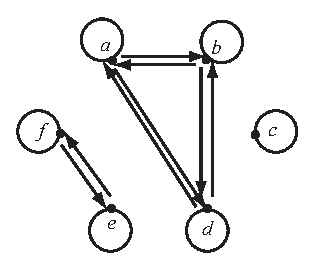
\includegraphics{figps-exer2-73.eps}}
\end{center}
\end{figure}

The equivalence class are
\[
[a] = [b] = [d] = \{a, b, d \}, \quad [c] = \{ c \}, \quad [e] = [f] = \{ e, f \}.
\]



\item Let   $A = \left\{ {0, 1, 2, 3,  \ldots , 999, 1000} \right\}$.  Define the relation  $R$  on  $A$  as follows:  For  $x, y \in A$,  $x \mathrel{R} y$ if and only if  $x$  and  $y$  have the same number of digits.

Let $x \in A$.  Since $x$ has the same number of digits as itself, the relation $\mathrel{R}$ is reflexive.  Now let $x, y, z \in A$.  If $x \mathrel{R} y$, then $x$  and  $y$  have the same number of digits.  Hence, $y$ and $x$ have the same number of digits and $y \mathrel{R} x$, and so $\mathrel{R}$ is symmetric.

If $x \mathrel{R} y$ and $y \mathrel{R} z$, then $x$  and  $y$  have the same number of digits and 
$y$  and  $z$  have the same number of digits.  Hence, $x$  and  $z$  have the same number of digits, and so $x \mathrel{R} z$.  Therefore, $\mathrel{R}$ is transitive.

The equivalence classes are:  
$\left\{ 0, 1, 2, \ldots , 9 \right\}$, $\left\{ 10, 11, 12, \ldots , 99 \right\}$, \\
$\left\{ 100, 101, 102, \ldots , 999 \right\}$, $\left\{ 1000 \right\}$.



\item The congruence classes for the relation of congruence modulo 5 on the set of integers are:

\begin{multicols}{2}$\left[ 0 \right] = \left\{ 5n \mid n \in \mathbb{Z} \right\}$

$\left[ 1 \right] = \left\{ 5n +1 \mid n \in \mathbb{Z} \right\}$

$\left[ 2 \right] = \left\{ 5n + 2 \mid n \in \mathbb{Z} \right\}$

$\left[ 3 \right] = \left\{ 5n + 3 \mid n \in \mathbb{Z} \right\}$

$\left[ 4 \right] = \left\{ 5n + 4 \mid n \in \mathbb{Z} \right\}$
\end{multicols}


\item \begin{enumerate}
\item Let $a, b, c \in \Z_9$.  Since $a^2 \equiv a^2 \pmod 9$, we see that $a \sim a$ and $\sim$ is reflexive.  Also, if $a \sim b$, then $a^2 \equiv b^2 \pmod 9$ and hence, by the symmetric property of congruence, $b^2 \equiv a^2 \pmod 9$.  This proves that $\sim$ is symmetric.  Finally, if $a \sim b$ and $b \sim c$, then 
$a^2 \equiv b^2 \pmod 9$ and $b^2 \equiv c^2 \pmod 9$.  By the transitive property of congruence, we conclude that $a^2 \equiv c^2 \pmod 9$ and hence, $a \sim c$.  This proves that $\sim$ is transitive.  The distinct equivalence classes are
\[
\{ 0, 3, 6 \}, \quad \{ 1, 8 \}, \quad \{2, 7 \}, \quad \{4, 5 \}.
\]
\item The proof that $\approx$ is an equivalence relation on $\Z_9$ is similar to the proof in Part~(a) that $\sim$ is an equivalence relation on $\Z_9$.  The distinct equivalence classes for $\approx$ are
\[
\{ 0, 3, 6 \}, \quad \{ 1, 4, 7 \}, \quad \{2, 5, 8 \}.
\]
\end{enumerate}



\item \begin{enumerate}
\item Let $x \in \left[ \dfrac{5}{7} \right]$.  Then $x - \dfrac{5}{7} \in \Z$, which means that there is an integer $m$ such that $x - \dfrac{5}{7} = m$, or $x = \dfrac{5}{7} + m$.  This proves that \linebreak
$x \in \left\{ \left. m + \dfrac{5}{7} \right| m \in \Z \right\}$ and, hence, that
$\left[ \dfrac{5}{7} \right] \subseteq \left\{ \left. m + \dfrac{5}{7} \right| m \in \Z \right\}$.

Now let $y \in \left\{ \left. m + \dfrac{5}{7} \right| m \in \Z \right\}$.  So there exists an integer $m$ such that $y = m + \dfrac{5}{7}$.  This means that $y - \dfrac{5}{7} = m$ and hence, $y - \dfrac{5}{7} \in \Z$.  Therefore, $y \sim \dfrac{5}{7}$, which means that $y \in \left[ \dfrac{5}{7} \right]$ and 
$\left\{ \left. m + \dfrac{5}{7} \right| m \in \Z \right\} \subseteq \left[ \dfrac{5}{7} \right]$.

\item If $a \in \Z$, then $[a] = \Z$.

\item Define $f\x \Z \to \left[ \dfrac{5}{7} \right]$ by $f(m) = m + \dfrac{5}{7}$ for each $m \in \Z$.  To prove $f$ is an injection, let $m, n \in \Z$ and assume that 
$f(m) = f(n)$.  Then $m + \dfrac{5}{7} = n + \dfrac{5}{7}$, which implies that $m = n$.  Therefore, $f$ is an injection.  To prove that $f$ is a surjection, let 
$y \in  \left[ \dfrac{5}{7} \right]$.  By Part~(a), there exists an $m \in \Z$ such that 
$y = m + \dfrac{5}{7}$.  We then see that $f(m) = y$ and $f$ is a surjection.
\end{enumerate}


\item \begin{enumerate}
\item If $x \in \R$, then $x - x = 0$ and hence, $x \sim x$.  So the relation $\sim$ is reflexive.  Now let $x, y \in \R$ and assume that $x \sim y$.  Then $x - y \in \Q$ and hence, $-(x - y) \in \Q$.  This means that $y - x \in \Q$ and hence, $y \sim x$.  Therefore, $\sim$ is symmetric.  Now let $x, y, z \in \R$ and assume that $x \sim y$ and 
$y \sim z$.  Then $x - y \in \Q$ and $y - z \in \Q$.  We can then conclude that 
$(x - y) + (y - z) \in \Q$ or that $x - z \in \Q$.  Hence, $x \sim z$ and the relation 
$\sim$ is transitive.

\item The following real numbers are in $\left[ \sqrt{2} \right]$:  $\sqrt{2}$, 
$1 + \sqrt{2}$, $-1 + \sqrt{2}$, $\dfrac{1}{2} + \sqrt{2}$, $\dfrac{2}{3} + \sqrt{2}$.

\item If $a \in \Q$, then $[a] = \Q$.

\item Let $x \in \left[ \sqrt{2} \right]$.  Then $x - \sqrt{2} \in \Q$, which means that there is a rational number $q$  such that $x - \sqrt{2} = q$, or $x = \sqrt{2} + q$.  This proves that $x \in \left\{ \left. r + \sqrt{2} \right| r \in \Q \right\}$ and, hence, that
$\left[ \sqrt{2} \right] \subseteq \left\{ \left. r + \sqrt{2} \right| r \in \Q \right\}$.

Now let $y \in \left\{ \left. r + \sqrt{2} \right| r \in \Q \right\}$.  So there exists a rationalnumber  $r$ such that $y = r + \sqrt{2}$.  This means that $y - \sqrt{2} = r$ and hence, $y - \sqrt{2} \in \Q$.  Therefore, $y \sim \sqrt{2}$, which means that 
$y \in \left[ \sqrt{2} \right]$ and 
$\left\{ \left. r + \sqrt{2} \right| r \in \Q \right\} \subseteq \left[ \sqrt{2} \right]$.

\item Define $f\x \Q \to \left[ \sqrt{2} \right]$ by $f(r) = r + \sqrt{2}$ for each $r \in \Q$.  To prove $f$ is an injection, let $p, r \in \Q$ and assume that 
$f(p) = f(r)$.  Then $p + \sqrt{2} = r + \sqrt{2}$, which implies that $p = r$.  Therefore, $f$ is an injection.  To prove that $f$ is a surjection, let 
$y \in  \left[ \sqrt{2} \right]$.  By Part~(d), there exists an $r \in \Q$ such that 
$y = r + \sqrt{2}$.  We then see that $f(r) = y$ and $f$ is a surjection.
\end{enumerate}


\item For this equivalence relation,
\begin{align*}
[0] &= \{ 5m \mid m \in \Z \} & [1] &= \{ 5m + 1 \mid m \in \Z \} \\
[2] &= \{ 5m + 2 \mid m \in \Z \}  &  [3] &= \{ 5m + 3 \mid m \in \Z \} \\
[4] &= \{ 5m + 4 \mid m \in \Z \}
\end{align*}



\item $A = \mathbb{Z} \times \left( {\mathbb{Z} - \left\{ 0 \right\}} \right)$.  For  
$\left( {a, b} \right), \left( {c, d} \right) \in A$,  
$\left( {a, b} \right) \approx \left( {c, d} \right)$ if and only if  $ad = bc$.

\begin{enumerate}
\item Let $\left( a, b \right) \in A$.  Since $ab = ba$, we see that 
$\left( a, b \right) \approx \left( a, b \right)$, and hence, $\approx$ is reflexive.

Now let $\left( a, b \right), \left( c, d \right) \in A$ and assume that 
$\left( a, b \right) \approx \left( c, d \right)$.  Then, $ad = bc$.  Hence, $cb = da$ and 
$\left( c, d \right) \approx \left( a, b \right)$.  Therefore, $\approx$ is symmetric.

Finally, let $\left( a, b \right), \left( c, d \right), \left( m, n \right) \in A$ and assume that 
$\left( a, b \right) \approx \left( c, d \right)$ and that 
$\left( c, d \right) \approx \left( m, n \right)$.  We conclude that
\begin{center}
$ad = bc$ and $cn = dm$.
\end{center}
We multiplby both sides of the first of these equations by $n$ to obtain $adn = bcn$.  We then subsitute $cn = dm$ on the right side of this equation to obtain
\[
adn = bdm.
\]
Since $d \ne 0$, we cancel $d$ from both sides of this equation to obtain $an = bm$.  This proves that $\left( a, b \right) \approx \left( m, n \right)$, and hence, $\approx$ is transitive.

\item In the proof that $\approx$ is an equivalence relation, we needed to have $d \ne 0$ to be able to cancel this from both sides of an equation.  This is why it was necessary to assume that second coordinate in the ordered pairs in $A$ are not zero.

\item $\left( a, b \right) \approx \left( 2, 3 \right)$ if and only if  $3a = 2b$.


\item $\left( a, b \right) \in \left[ \left( 2, 3 \right) \right]$ if and only if $3a = 2b$.  All examples must satisfy this equation.

\item $\left[ \left( 2, 3 \right) \right] = \left\{ \left( a, b \right) \in A \mid 3a = 2b \right\}$.
\end{enumerate}



\item The result stated in the exercise is incorrect.  The relation $\sim$ is not an equivalence relation.  It can be redefined to be an equivalence relation as follows:
\begin{center}
For $x, y \in \R$, $x \sim y$ if and only if either $x = 0$ and $y = 0$ or $xy > 0$.
\end{center}
In this case, the equivalence classes are
\[
\{ 0 \}, \quad \{ x \in \R \mid x > 0 \}, \quad \{ x \in \R \mid x < 0 \}.
\]



\item \begin{enumerate}
\item $[ (0, 0) ] = \{ (0, 0) \}$.

\item $[ (2, 3) ] = \{ (x, y) \in \R \times \R \mid x^2 + y^2 = 13$.  This equivalence class consists of the points in the plane on a circle of radius $\sqrt{13}$ centered at the origin.

\item Except for $[(0, 0)]$, the equivalence classes for this equivalence relation consist of points on a circle whose center is the origin.

\item Let $C_0 = \{ (0, 0) \}$ and for each positive real number $r$, let $C_r$ be the set of points on the circle of radius $r$ whose center is at the origin.  Then
\[
C_r = [ (r, 0) ].
\]
Now let $(a, b) \in \R \times \R$ and let $r = \sqrt{a^2 + b^2}$.  Then, $[a, b] = [r, 0]$ and so the set of all equivalence classes of $\sim$ is 
\[
T =  \{ C_r \mid r \in \R^* \}.
\]
Now define $f\x \R^* \to T$ by $f(r) = C_r$.  The work above shows that $f$ is a surjection.  So let $r, s \in \R^*$ and assume that $f(r) = f(s)$.  This means that 
$C_r = C_s$ and this implies that $r^2 = s^2$ or that $r = s$.  So the function $f$ is an injection.
\end{enumerate}





\item \begin{enumerate}
\item For each  $a, b \in A$,    $a\nsim b$ if and only if   
        $\left[ a \right] \cap \left[ b \right] = \emptyset $.

\textbf{\emph{Proof}.}  If $a\nsim b$, then $\left[ a \right] \ne \left[ b \right]$.  Hence, by Theorem~\ref{T:propsofequivclasses}, $\left[ a \right] \cap \left[ b \right] = \emptyset $.  In addition, if $a \sim b$, then by Theorem~\ref{T:propsofequivclasses}, 
$\left[ a \right] = \left[ b \right]$ and so, 
$\left[ a \right] \cap \left[ b \right] \ne \emptyset $.  This proves that if $a \sim b$, then , $\left[ a \right] \cap \left[ b \right] \ne \emptyset $ and hence that if 
$\left[ a \right] \cap \left[ b \right] = \emptyset $, then $a \nsim b$.

\item Statement~(3) in Theorem~\ref{T:propsofequivclasses} is logically equivalent to, 
``For each  $a, b \in A$,   if  $\left[ a \right] \ne \left[ b \right]$, then   
$\left[ a \right] \cap \left[ b \right] = \emptyset $.''  This uses the following logical equivalency:  $\mynot P \vee Q \equiv P \to Q$.

\item This is the contrapositive of the statement in~(b).
\end{enumerate}
\end{enumerate}


\subsection*{Explorations and Activities}
\setcounter{oldenumi}{\theenumi}
\begin{enumerate} \setcounter{enumi}{\theoldenumi}
\item Let  $A = \left\{ {a, b, c, d, e} \right\}$ and let  
$\mathcal{C} = \left\{ {\left\{ {a, b, c} \right\}, \left\{ {d, e} \right\}} \right\}$. 

\begin{enumerate}
\item $\mathcal{C}$ is a partition of $A$  since each set in  $\mathcal{C}$  is nonempty, each element of  $A$  is in one set contained in  $\mathcal{C}$ , and the two unequal subsets  of  $A$  contained in  $\mathcal{C}$  are disjoint.

\item Let  $x \in A$.  Then ,  $x \sim x$ since there exists a set  $T$  in  $\mathcal{C}$  such that  $x \in T$ and  $x \in T$.  This means that the relation  $\sim$  is reflexive on  $A$.
\vskip6pt
Now let  $x, y \in A$ and assume that  $x \sim y$.  Then, there exists a set  $T$  in  
$\mathcal{C}$  such that  $x \in T$ and  $y \in T$.  But then,  $y \in T$ and  $x \in T$, and hence,  $y \sim x$.  Therefore, the relation  $\sim$  is symmetric.
\vskip6pt

Finally, let  $x, y, z \in A$  and assume that  $x \sim y$  and  $y \sim z$.  Then, there exists a set  $T$  in  $\mathcal{C}$  such that  $x \in T$ and  $y \in T$  and  there exists a set  $V$  in  $\mathcal{C}$  such that  $y \in V$ and  $z \in V$.  Since  $y \in T \cap V$, we can conclude that  $T \cap V \ne \emptyset $.  Since  $T$  and  $V$  are sets in the partition  $\mathcal{C}$ , this implies that  $T = V$.  Therefore,  $x \in T$ and  $z \in T$ and hence, the relation  $\sim$  is transitive. So, we have proven that  $\sim$  is an equivalence relation on  $A$.
\vskip6pt

The equivalence classes for $\mathcal{C}$ are:  $\left[ a \right] = \left[ b \right] = \left[ c \right] = \left\{ {a, b, c} \right\}$  and   
$\left[ d \right] = \left[ e \right] = \left\{ {d, e} \right\}$.  These are the same subsets of 
$A$ that form the partition $\mathcal{C}$.


\item Repeat the proof in Part (b).

\item Let  $a \in A$  and let  $T \in \mathcal{C}$ such that  $a \in T$.  Now assume that  
$x \in \left[ a \right]$.  Then,  $x \sim a$ and hence,  there exists a set  $V$  in  
$\mathcal{C}$  such that  $x \in V$ and  $a \in V$.  Since  $a \in T \cap V$, we know that  
$T \cap V \ne \emptyset $, and  since  $T$  and  $V$  are sets in the partition  $\mathcal{C}$, this implies that  $T = V$.   Therefore, $x \in T$, and we conclude that  
$\left[ a \right] \subseteq T$.

Now let  $x \in T$.  Then by the definition of  $\sim$,  $x \sim a$ and  
$x \in \left[ a \right]$.  This proves that  $T \subseteq \left[ a \right]$ and hence that  
$\left[ a \right] = T$.
\end{enumerate}



\item Let $I$ be the identity matrix in $\mathcal{M}_{n, n}\left( \R \right)$.
\begin{enumerate}
\item For $A \in \mathcal{M}_{n, n}\left( \R \right)$, $A = IAI^{-1}$ and so $A \sim A$.  Hence, the relation $\sim$ is reflexive.  

Now let $A, B, C \in \mathcal{M}_{n, n}\left( \R \right)$.  First assume that $A \sim B$.  Then there exists an invertible matrix $P$ in $\mathcal{M}_{n, n}\left( \R \right)$ such that $B = PAP^{-1}$.  From linear algebra, we know that $P^{-1}$ is invertible and so
\begin{align*}
P^{-1}BP &= P^{-1} \left( PAP^{-1} \right) P \\
         &= \left( P^{-1}P \right) A \left( P^{-1} P \right) \\
         &= A.
\end{align*}
Hence, $B \sim A$ and the relation $\sim$ is symmetric.  Now assume that $A \sim B$ and 
$B \sim C$.  Then there exist invertible matrices $P$ and $Q$ in 
$\mathcal{M}_{n, n}\left( \R \right)$ such that $B = PAP^{-1}$ and $C = QBQ^{-1}$.  We then see that
\begin{align*}
C &= Q \left( PAP^{-1} \right) Q^{-1} \\
  &= \left(QP \right) A \left( P^{-1} Q^{-1} \right) \\
  &= \left( QP \right) A \left( QP \right)^{-1}.
\end{align*}
This proves that the relation $\sim$ is transitive and hence, $\sim$ is an equivalence relation.

\item Let $A, B, C \in \mathcal{M}_{n, n}\left( \R \right)$.  Since $\det(A) = \det(A)$, we see that $A \mathrel{R} A$ and $R$ is reflexive.  In addition, if $\det(A) = \det(B)$, then $\det(B) = \det(A)$.  This can be used to prove that $R$ is symmetric.  Finally, if 
$\det(A) = \det(B)$ and $\det(B) = \det(C)$, then $\det(A) = \det(C)$.  This can be used to prove that $R$ is transitive.

\item For this problem, $\sim$ is an equivalence relation on $\R$. Let $A, B, C \in \mathcal{M}_{n, n}\left( \R \right)$.  Since $\det(A) \in \R$ and $\sim$ is reflexive, 
$\det(A) \sim \det(A)$.  This proves that $\approx$ is reflexive on 
$\mathcal{M}_{n, n}\left( \R \right)$.  Now assume that $A \approx B$.  Then $\det(A) \sim \det(B)$.  Since $\sim$ is symmetric, we conclude that $\det(B) \sim \det(A)$ and hence, 
$B \approx A$.  This proves that $\approx$ is symmetric.

Finally, assume that $A \approx B$ and $B \approx C$.  Then $\det(A) \sim \det(B)$ and 
$\det(B) \sim \det(C)$.  Since $\sim$ is transitive, we can conclude that 
$\det(A) \sim \det(C)$.  Hence, $A \approx C$ and so $\approx$ is transitive.  This proves that $\approx$ is an equivalence relation on $\mathcal{M}_{n, n}\left( \R \right)$.
\end{enumerate}

\end{enumerate}
\hbreak
\endinput

\section*{Section \ref{S:modulararithmetic} Modular Arithmetic}

\begin{enumerate}

\item \begin{enumerate}
\item
%\begin{center}
\begin{tabular}{ c | c  c  c  c p{0.5in} c | c  c  c c}
$\oplus$ & $\left[ 0 \right]$ & $\left[ 1 \right]$ & $\left[ 2 \right]$ & $\left[ 3 \right]$ & &   $\odot$ & $\left[ 0 \right]$ & $\left[ 1 \right]$ & $\left[ 2 \right]$ & $\left[ 3 \right]$  \\ \cline{1-5} \cline{7-11}

$\left[ 0 \right]$ & $\left[ 0 \right]$ & $\left[ 1 \right]$ & $\left[ 2 \right]$ & $\left[ 3 \right]$&  & 
$\left[ 0 \right]$ & $\left[ 0 \right]$ & $\left[ 0 \right]$ & $\left[ 0 \right]$ & $\left[ 0 \right]$ 
\\ 

$\left[ 1 \right]$ & $\left[ 1 \right]$ & $\left[ 2 \right]$ & $\left[ 3 \right]$ & $\left[ 0 \right]$ &  & 
$\left[ 1 \right]$ & $\left[ 0 \right]$ & $\left[ 1 \right]$ & $\left[ 2 \right]$ & $\left[ 3 \right]$
\\ 

$\left[ 2 \right]$ & $\left[ 2 \right]$ & $\left[ 3 \right]$ & $\left[ 0 \right]$ & $\left[ 1 \right]$ &  & 
$\left[ 2 \right]$ & $\left[ 0 \right]$ & $\left[ 2 \right]$ & $\left[ 0 \right]$ & $\left[ 2 \right]$
\\ 

$\left[ 3 \right]$ & $\left[ 3 \right]$ & $\left[ 0 \right]$ & $\left[ 1 \right]$ & $\left[ 2 \right]$ &  & 
$\left[ 3 \right]$ & $\left[ 0 \right]$ & $\left[ 3 \right]$ & $\left[ 2 \right]$ & $\left[ 1 \right]$
\\ 

\end{tabular}
%\end{center}

\item
\begin{tabular}{ c | c  c  c  c  c  c  c}
$\oplus$ & $\left[ 0 \right]$ & $\left[ 1 \right]$ & $\left[ 2 \right]$ & $\left[ 3 \right]$ & 
$\left[ 4 \right]$ & $\left[ 5 \right]$ & $\left[ 6 \right]$  \\ \hline

$\left[ 0 \right]$ & $\left[ 0 \right]$ & $\left[ 1 \right]$ & $\left[ 2 \right]$ & 
$\left[ 3 \right]$ & $\left[ 4 \right]$ & $\left[ 5 \right]$ & $\left[ 6 \right]$  \\ 

$\left[ 1 \right]$ & $\left[ 1 \right]$ & $\left[ 2 \right]$ & $\left[ 3 \right]$ & 
$\left[ 4 \right]$ & $\left[ 5 \right]$ & $\left[ 6 \right]$ & $\left[ 0 \right]$  \\ 

$\left[ 2 \right]$ & $\left[ 2 \right]$ & $\left[ 3 \right]$ & $\left[ 4 \right]$ & 
$\left[ 5 \right]$ & $\left[ 6 \right]$ & $\left[ 0 \right]$ & $\left[ 1 \right]$  \\ 

$\left[ 3 \right]$ & $\left[ 3 \right]$ & $\left[ 4 \right]$ & $\left[ 5 \right]$ & 
$\left[ 6 \right]$ & $\left[ 0 \right]$ & $\left[ 1 \right]$ & $\left[ 2 \right]$ \\ 

$\left[ 4 \right]$ & $\left[ 4 \right]$ & $\left[ 5 \right]$ & $\left[ 6 \right]$ & 
$\left[ 0 \right]$ & $\left[ 1 \right]$ & $\left[ 2 \right]$ & $\left[ 3 \right]$  \\ 

$\left[ 5 \right]$ & $\left[ 5 \right]$ & $\left[ 6 \right]$ & $\left[ 0 \right]$ & 
$\left[ 1 \right]$ & $\left[ 2 \right]$ & $\left[ 3 \right]$ & $\left[ 4 \right]$  \\ 

$\left[ 6 \right]$ & $\left[ 6 \right]$ & $\left[ 0 \right]$ & $\left[ 1 \right]$ & 
$\left[ 2 \right]$ & $\left[ 3 \right]$ & $\left[ 4 \right]$ & $\left[ 5 \right]$  \\ 
\end{tabular}

\vskip 9pt

\begin{tabular}{ c | c  c  c  c  c  c  c}
$\odot$ & $\left[ 0 \right]$ & $\left[ 1 \right]$ & $\left[ 2 \right]$ & $\left[ 3 \right]$ & 
$\left[ 4 \right]$ & $\left[ 5 \right]$ & $\left[ 6 \right]$  \\ \hline

$\left[ 0 \right]$ & $\left[ 0 \right]$ & $\left[ 0 \right]$ & $\left[ 0 \right]$ & 
$\left[ 0 \right]$ & $\left[ 0 \right]$ & $\left[ 0 \right]$ & $\left[ 0 \right]$  \\ 

$\left[ 1 \right]$ & $\left[ 1 \right]$ & $\left[ 2 \right]$ & $\left[ 3 \right]$ & 
$\left[ 4 \right]$ & $\left[ 5 \right]$ & $\left[ 6 \right]$ & $\left[ 0 \right]$  \\ 

$\left[ 2 \right]$ & $\left[ 0 \right]$ & $\left[ 2 \right]$ & $\left[ 4 \right]$ & 
$\left[ 6 \right]$ & $\left[ 1 \right]$ & $\left[ 3 \right]$ & $\left[ 5 \right]$  \\ 

$\left[ 3 \right]$ & $\left[ 0 \right]$ & $\left[ 3 \right]$ & $\left[ 6 \right]$ & 
$\left[ 2 \right]$ & $\left[ 5 \right]$ & $\left[ 1 \right]$ & $\left[ 4 \right]$  \\ 

$\left[ 4 \right]$ & $\left[ 0 \right]$ & $\left[ 4 \right]$ & $\left[ 1 \right]$ & 
$\left[ 5 \right]$ & $\left[ 2 \right]$ & $\left[ 6 \right]$ & $\left[ 3 \right]$  \\ 

$\left[ 5 \right]$ & $\left[ 0 \right]$ & $\left[ 5 \right]$ & $\left[ 3 \right]$ & 
$\left[ 1 \right]$ & $\left[ 6 \right]$ & $\left[ 4 \right]$ & $\left[ 2 \right]$  \\ 

$\left[ 6 \right]$ & $\left[ 0 \right]$ & $\left[ 6 \right]$ & $\left[ 5 \right]$ & 
$\left[ 4 \right]$ & $\left[ 3 \right]$ & $\left[ 2 \right]$ & $\left[ 1 \right]$  \\ 
\end{tabular}

\item
\begin{tabular}{ c | c  c  c  c  c  c  c c}
$\oplus$ & $\left[ 0 \right]$ & $\left[ 1 \right]$ & $\left[ 2 \right]$ & $\left[ 3 \right]$ & 
$\left[ 4 \right]$ & $\left[ 5 \right]$ & $\left[ 6 \right]$ & $\left[ 7 \right]$  \\ \hline

$\left[ 0 \right]$ & $\left[ 0 \right]$ & $\left[ 1 \right]$ & $\left[ 2 \right]$ & 
$\left[ 3 \right]$ & $\left[ 4 \right]$ & $\left[ 5 \right]$ & $\left[ 6 \right]$ & 
$\left[ 7 \right]$  \\ 

$\left[ 1 \right]$ & $\left[ 1 \right]$ & $\left[ 2 \right]$ & $\left[ 3 \right]$ & 
$\left[ 4 \right]$ & $\left[ 5 \right]$ & $\left[ 6 \right]$ & $\left[ 7 \right]$ & 
$\left[ 0 \right]$ \\ 

$\left[ 2 \right]$ & $\left[ 2 \right]$ & $\left[ 3 \right]$ & $\left[ 4 \right]$ & 
$\left[ 5 \right]$ & $\left[ 6 \right]$ & $\left[ 7 \right]$ & $\left[ 0 \right]$ & 
$\left[ 1 \right]$  \\ 

$\left[ 3 \right]$ & $\left[ 3 \right]$ & $\left[ 4 \right]$ & $\left[ 5 \right]$ & 
$\left[ 6 \right]$ & $\left[ 7 \right]$ & $\left[ 0 \right]$ & $\left[ 1 \right]$ & 
$\left[ 2 \right]$  \\ 

$\left[ 4 \right]$ & $\left[ 4 \right]$ & $\left[ 5 \right]$ & $\left[ 6 \right]$ & 
$\left[ 7 \right]$ & $\left[ 0 \right]$ & $\left[ 1 \right]$ & $\left[ 2 \right]$ & 
$\left[ 3 \right]$  \\ 

$\left[ 5 \right]$ & $\left[ 5 \right]$ & $\left[ 6 \right]$ & $\left[ 7 \right]$ & 
$\left[ 0 \right]$ & $\left[ 1 \right]$ & $\left[ 2 \right]$ & $\left[ 3 \right]$ & 
$\left[ 4 \right]$  \\ 

$\left[ 6 \right]$ & $\left[ 6 \right]$ & $\left[ 7 \right]$ & $\left[ 0 \right]$ & 
$\left[ 1 \right]$ & $\left[ 2 \right]$ & $\left[ 3 \right]$ & $\left[ 4 \right]$ & 
$\left[ 5 \right]$  \\ 

$\left[ 7 \right]$ & $\left[ 7 \right]$ & $\left[ 0 \right]$ & $\left[ 1 \right]$ & 
$\left[ 2 \right]$ & $\left[ 3 \right]$ & $\left[ 4 \right]$ & $\left[ 5 \right]$ & 
$\left[ 6 \right]$  \\ 
\end{tabular}

\vskip 9pt

\begin{tabular}{ c | c  c  c  c  c  c  c c}
$\odot$ & $\left[ 0 \right]$ & $\left[ 1 \right]$ & $\left[ 2 \right]$ & $\left[ 3 \right]$ & 
$\left[ 4 \right]$ & $\left[ 5 \right]$ & $\left[ 6 \right]$ & $\left[ 7 \right]$  \\ \hline

$\left[ 0 \right]$ & $\left[ 0 \right]$ & $\left[ 0 \right]$ & $\left[ 0 \right]$ & 
$\left[ 0 \right]$ & $\left[ 0 \right]$ & $\left[ 0 \right]$ & $\left[ 0 \right]$ & 
$\left[ 0 \right]$  \\ 

$\left[ 1 \right]$ & $\left[ 0 \right]$ & $\left[ 1 \right]$ & $\left[ 2 \right]$ & 
$\left[ 3 \right]$ & $\left[ 4 \right]$ & $\left[ 5 \right]$ & $\left[ 6 \right]$ & 
$\left[ 7 \right]$ \\ 

$\left[ 2 \right]$ & $\left[ 0 \right]$ & $\left[ 2 \right]$ & $\left[ 4 \right]$ & 
$\left[ 6 \right]$ & $\left[ 0 \right]$ & $\left[ 2 \right]$ & $\left[ 4 \right]$ & 
$\left[ 6 \right]$  \\ 

$\left[ 3 \right]$ & $\left[ 0 \right]$ & $\left[ 3 \right]$ & $\left[ 6 \right]$ & 
$\left[ 1 \right]$ & $\left[ 4 \right]$ & $\left[ 7 \right]$ & $\left[ 2 \right]$ & 
$\left[ 5 \right]$  \\ 

$\left[ 4 \right]$ & $\left[ 0 \right]$ & $\left[ 4 \right]$ & $\left[ 0 \right]$ & 
$\left[ 4 \right]$ & $\left[ 0 \right]$ & $\left[ 4 \right]$ & $\left[ 0 \right]$ & 
$\left[ 4 \right]$  \\ 

$\left[ 5 \right]$ & $\left[ 0 \right]$ & $\left[ 5 \right]$ & $\left[ 2 \right]$ & 
$\left[ 7 \right]$ & $\left[ 4 \right]$ & $\left[ 1 \right]$ & $\left[ 6 \right]$ & 
$\left[ 3 \right]$  \\ 

$\left[ 6 \right]$ & $\left[ 0 \right]$ & $\left[ 6 \right]$ & $\left[ 4 \right]$ & 
$\left[ 2 \right]$ & $\left[ 0 \right]$ & $\left[ 6 \right]$ & $\left[ 4 \right]$ & 
$\left[ 2 \right]$  \\ 

$\left[ 7 \right]$ & $\left[ 0 \right]$ & $\left[ 7 \right]$ & $\left[ 6 \right]$ & 
$\left[ 5 \right]$ & $\left[ 4 \right]$ & $\left[ 3 \right]$ & $\left[ 2 \right]$ & 
$\left[ 1 \right]$  \\ 
\end{tabular}
\end{enumerate}




\item \begin{enumerate}
\item $\left[ x \right] = \left[ 1 \right]$ or $\left[ x \right] = \left[ 3 \right]$. 

\item $\left[ x \right] = \left[ 1 \right]$, $\left[ x \right] = \left[ 3 \right]$, 
$\left[ x \right] = \left[ 5 \right]$, or $\left[ x \right] = \left[ 7 \right]$.

\item $\left[ x \right] = \left[ 1 \right]$, $\left[ x \right] = \left[ 2 \right]$, 
$\left[ x \right] = \left[ 3 \right]$, or $\left[ x \right] = \left[ 4 \right]$.

\item The equation has no solution.

\item $\left[ x \right] = \left[ 2 \right]$ or $\left[ x \right] = \left[ 3 \right]$.

\item $\left[ x \right] = \left[ 1 \right]$.

\item The equation has no solution.

\item The equation has no solution.
\end{enumerate}



\item \begin{enumerate}
\item The statement is false.  By using the multiplication table for $\mathbb{Z}_6$, we see that a counterexample is $\left[ a \right] = \left[ 2 \right]$.

\item The statement is true.  By using the multiplication table for $\mathbb{Z}_5$, we see that:

\begin{multicols}{2}
\begin{list}{}
\item $\left[ 1 \right] \odot \left[ 1 \right] = \left[ 1 \right]$.

\item $\left[ 2 \right] \odot \left[ 3 \right] = \left[ 1 \right]$.

\item $\left[ 3 \right] \odot \left[ 2 \right] = \left[ 1 \right]$.

\item $\left[ 4 \right] \odot \left[ 4 \right] = \left[ 1 \right]$.
\end{list}
\end{multicols}
\end{enumerate}



\item \begin{enumerate}
\item The statement is false.  A counterexample is $\left[ a \right] = \left[ 2 \right]$ and $\left[ b \right] = \left[ 3 \right]$.

\item The statement is true.  By using the multiplication table for $\mathbb{Z}_5$, we see that there are no entries equal to $\left[ 0 \right]$ when $\left[ a \right] \ne \left[ 0 \right]$ and 
$\left[ b \right] \ne \left[ 0 \right]$.
\end{enumerate}



\item \begin{enumerate}
\item The proof consists of the following computations:
\begin{multicols}{2}
\begin{list}{}
\item $[ 1 ]^2 = [ 1 ]$
\item $[ 2 ]^2 = [ 4 ]$
\item $[ 3 ]^2 = [ 9 ] = [ 4 ]$
\item $[ 4 ]^2 = [ 16 ] = [ 1 ]$.
\end{list}
\end{multicols}

\item If there exists an integer $a$ such that $a^2 = 5,158,232,468,953,153$, then 
$a^2 \equiv 3 \pmod 5$.  This contradicts the result in Part~(a).  Therefore, no such integer exists.
\end{enumerate}




\item The key idea in the inductive step of the proof is that if
\[
10^k \equiv 1 \pmod 9,
\]
then $10 \cdot 10^k \equiv 10 \cdot 1 \pmod 9$.  This proves that $10^{k+1} \equiv 10 \pmod 9$ and since $10 \equiv 1 \pmod 9$, we conclude that $10^{k+1} \equiv 1 \pmod 9$.


\item The key idea in the inductive step of the proof is that if
\[
10^k \equiv 1 \pmod 3,
\]
then $10 \cdot 10^k \equiv 10 \cdot 1 \pmod 3$.  This proves that $10^{k+1} \equiv 10 \pmod 3$ and since $10 \equiv 1 \pmod 3$, we conclude that $10^{k+1} \equiv 1 \pmod 3$.


\item \begin{enumerate}
\item 
\begin{align}
  \left[ n \right] &= \left[ {\left( {a_k  \times 10^k } \right) + \left( {a_{k - 1}  \times 10^{k - 1} } \right) +  \cdots  + \left( {a_1  \times 10^1 } \right) + \left( {a_0  \times 10^0 } \right)} \right] \notag \\ 
   &= \left[ {a_k  \times 10^k } \right] \oplus \left[ {a_{k - 1}  \times 10^{k - 1} } \right] \oplus  \cdots  \oplus \left[ {a_1  \times 10^1 } \right] \oplus \left[ {a_0  \times 10^0 } \right] \notag \\
  &= \left( {\left[ {a_k } \right] \otimes \left[ {10^k } \right]} \right) \oplus \left( {\left[ {a_{k - 1} } \right] \otimes \left[ {10^{k - 1} } \right]} \right) \oplus  \cdots \notag \\ 
  & \hspace{5cm} \oplus \left( {\left[ {a_1 } \right] \otimes \left[ {10^1 } \right]} \right) \oplus \left( {\left[ {a_0 } \right] \otimes \left[ {10^0 } \right]} \right) \notag  
\end{align}

So, the result in Exercise~(\ref{exer:poweroftenmod3}) implies that
\begin{align} \notag
[ n ] &= \left( {[ {a_k } ] \odot [ 1 ]} \right) \oplus \left( {[ {a_{k - 1} } ] \odot [ 1 ]} \right) \oplus  \cdots  \oplus \left( {[ {a_1 } ] \odot [ 1 ]} \right) \oplus \left( {[ {a_0 } ] \odot [ 1 ]} \right)  \notag \\ 
                 &= [ {a_k } ] \oplus [ {a_{k - 1} } ] \oplus  \cdots  \oplus [ {a_1 } ] \oplus [ {a_0 } ] \notag \\ 
                 &= [ {a_k  + a_{k - 1}  +  \cdots  + a_1  + a_0 } ]. \notag \\
%\label{eq:divideby9-5} \\
                 &= [ s( n ) ]. \notag
\end{align}
\item Converting the result in Part~(a) to a congruence, we see that \\ 
$n \equiv s(n)  \pmod 3$.

\item By Part~(b),  $n \equiv 0 \pmod 3$  if and only if  
$ s(n)  \equiv 0 \pmod 3$.  This means that $3 \mid n$ if and only if  
$5 \mid s(n) $.
\end{enumerate}



\item The key idea in the inductive step of the proof is that if
\[
10^k \equiv 0 \pmod 5,
\]
then $10 \cdot 10^k \equiv 10 \cdot 0 \pmod 5$.  This proves that $10^{k+1} \equiv 0 \pmod 5$.



\item \begin{enumerate}
\item 
\begin{align}
  \left[ n \right] &= \left[ {\left( {a_k  \times 10^k } \right) + \left( {a_{k - 1}  \times 10^{k - 1} } \right) +  \cdots  + \left( {a_1  \times 10^1 } \right) + \left( {a_0  \times 10^0 } \right)} \right] \notag \\ 
   &= \left[ {a_k  \times 10^k } \right] \oplus \left[ {a_{k - 1}  \times 10^{k - 1} } \right] \oplus  \cdots  \oplus \left[ {a_1  \times 10^1 } \right] \oplus \left[ {a_0  \times 10^0 } \right] \notag \\
  &= \left( {\left[ {a_k } \right] \otimes \left[ {10^k } \right]} \right) \oplus \left( {\left[ {a_{k - 1} } \right] \otimes \left[ {10^{k - 1} } \right]} \right) \oplus  \cdots \notag \\ 
  & \hspace{5cm} \oplus \left( {\left[ {a_1 } \right] \otimes \left[ {10^1 } \right]} \right) \oplus \left( {\left[ {a_0 } \right] \otimes \left[ {10^0 } \right]} \right) \notag  
\end{align}

So, the result in Exercise~(\ref{exer:poweroftenmod5}) implies that
\[
\begin{aligned}
  \left[ n \right] &= \left( {\left[ {a_0 } \right] \otimes \left[ {10^0 } \right]} \right) \\ 
                   &= \left[ {a_0 } \right] \\ 
\end{aligned}
\]
\item Converting the result in Part~(a) to a congruence, we see that \\ 
$n \equiv  {a_0 }  \pmod 5$.

\item By Part~(b),  $n \equiv 0 \pmod 5$  if and only if  
$ {a_0 }  \equiv 0 \pmod 5$.  This means that $5 \mid n$ if and only if  
$5 \mid  {a_0 } $.
\end{enumerate}



\item The key idea in the inductive step of the proof is that if
\[
10^k \equiv 0 \pmod 4,
\]
then $10 \cdot 10^k \equiv 10 \cdot 0 \pmod 4$.  This proves that $10^{k+1} \equiv 0 \pmod 4$.

\item \begin{enumerate}
\item Following is an outline of a proof.
\[
  \left[ n \right] = \left( {\left[ {a_k } \right] \otimes \left[ {10^k } \right]} \right) \oplus \left( {\left[ {a_{k - 1} } \right] \otimes \left[ {10^{k - 1} } \right]} \right) \oplus  \cdots  \oplus \left( {\left[ {a_1 } \right] \otimes \left[ {10^1 } \right]} \right) \oplus \left( {\left[ {a_0 } \right] \otimes \left[ {10^0 } \right]} \right)
\]
So, the result in Exercise~(\ref{exer:poweroftenmod4}) implies that
\[
\begin{aligned}
  \left[ n \right] &= \left( {\left[ {a_2 } \right] \otimes \left[ {10^2 } \right]} \right) \oplus \left( {\left[ {a_1 } \right] \otimes \left[ {10^1 } \right]} \right) \oplus \left( {\left[ {a_0 } \right] \otimes \left[ {10^0 } \right]} \right) \\ 
   &= \left[ {10a_1  + a_0 } \right] \\ 
\end{aligned}
\]

\item Converting this result to a congruence, we see that  
\[
n \equiv \left( {10a_1  + a_0 } \right) \pmod 8.
\]

\item Hence, $4 \mid n$ if and only if $4 \mid \left( {10a_1  + a_0 } \right)$.
\end{enumerate}




\item The key idea in the inductive step of the proof is that if
\[
10^k \equiv 0 \pmod 8,
\]
then $10 \cdot 10^k \equiv 10 \cdot 0 \pmod 8$.  This proves that $10^{k+1} \equiv 0 \pmod 8$.

\item The divisibility test for 8 is:   $8 \mid n$ if and only if  
$8 \mid \left( {100a_2 + 10a_1  + a_0 } \right)$.  Following is an outline of a proof.

\[
  \left[ n \right] = \left( {\left[ {a_k } \right] \otimes \left[ {10^k } \right]} \right) \oplus \left( {\left[ {a_{k - 1} } \right] \otimes \left[ {10^{k - 1} } \right]} \right) \oplus  \cdots  \oplus \left( {\left[ {a_1 } \right] \otimes \left[ {10^1 } \right]} \right) \oplus \left( {\left[ {a_0 } \right] \otimes \left[ {10^0 } \right]} \right)
\]
So, the result in Exercise~(\ref{exer:poweroftenmod8}) implies that
\[
\begin{aligned}
  \left[ n \right] &= \left( {\left[ {a_2 } \right] \otimes \left[ {10^2 } \right]} \right) \oplus \left( {\left[ {a_1 } \right] \otimes \left[ {10^1 } \right]} \right) \oplus \left( {\left[ {a_0 } \right] \otimes \left[ {10^0 } \right]} \right) \\ 
   &= \left[ {100a_2 + 10a_1  + a_0 } \right] \\ 
\end{aligned}
\]
Converting this result to a congruence, we see that  
\[
n \equiv \left( {100a_2 + 10a_1  + a_0 } \right) \pmod 8.
\]
Hence, $8 \mid n$ if and only if $8 \mid \left( {100a_2 + 10a_1  + a_0 } \right)$.




\item The key idea in the inductive step of the proof is that if
\[
10^k \equiv \left( -1 \right)^k \pmod {11},
\]
then $10 \cdot 10^k \equiv 10 \cdot \left( -1 \right)^k \pmod {11}$.  Since 
$10 \equiv -1 \pmod {11}$, we can conclude that
\[
10^{k+1} \equiv \left( -1 \right) \cdot \left( -1 \right)^k \pmod {11},
\]
and hence that $10^{k+1} \equiv \left( -1 \right)^{k+1} \pmod {11}$.

\item \begin{enumerate}
\item If  $n = \sum\limits_{j = 0}^k \left( {a_j \times 10^j} \right)$, then 
$n \equiv \sum\limits_{j = 0}^k \left[ { a_j \times 10^j \pmod {11}} \right]$. Therefore,  
$n \equiv \sum\limits_{j = 0}^k \left[ {\left( { - 1} \right)^j a_j } \pmod {11} \right]$, and hence, \\$n \equiv \sum\limits_{j = 0}^k {\left( { - 1} \right)^j a_j } \pmod {11}$.

\item This is a direct consequence of Part~(a).

\item By Part~(b), $\left[ n \right] = \left[ 0 \right]$ if and only if 
$\left[ {\sum\limits_{j = 0}^k {\left( { - 1} \right)^j a_j } }\right] = \left[ 0 \right]$.  This means that  $11 \mid n$ if and only if  
$11 \mid \sum\limits_{j = 0}^k {\left( { - 1} \right)^j a_j }$. 
\end{enumerate}

\item \begin{enumerate}
\item First, use the multiplication table to show that if $\left[ x \right] \in \mathbb{Z}_3$ and 
$\left[ x \right] \ne \left[ 0 \right]$, then $\left[ x \right]^2 = \left[ 1 \right]$.  This can then be used to prove the contrapositive: If $\left[ a \right] \ne \left[ 0 \right]$ and 
$\left[ b \right] \ne \left[ 0 \right]$, then 
$\left[ a \right]^2 + \left[ b \right]^2 \ne \left[ 0 \right]$.

\item By translating the statement in Part~(a) from congruence classes to congruence modulo 3, we see that if  $\left( {a^2  + b^2 } \right) \equiv 0 \pmod 3$, then  
$a \equiv 0 \pmod 3$  and  $b \equiv 0 \pmod 3$.

\item This follows directly from Part~(b) since $x \equiv 0 \pmod 3$ if and only if $3 \mid x$.
\end{enumerate}

\item Examine all 10 cases in $\mathbb{Z}_{10}$ to prove that if 
$\left[ x \right] \in \mathbb{Z}_{10}$, then $\left[ x \right]^4$ must be $\left[ 0 \right]$, 
$\left[ 1 \right]$, $\left[ 5 \right]$, or $\left[ 6 \right]$.  Then, construct an addition table for these 4 values using addition modulo 10.  The only entries in this table will be 
$\left[ 0 \right]$, $\left[ 1 \right]$, $\left[ 2 \right]$, or $\left[ 5 \right]$, 
$\left[ 6 \right]$, and $\left[ 7 \right]$.  This proves that $\left [ a \right]$ must be one of these 6 congruence classes and hence $a$ must be congruent modulo 10 to 0, 1, 2, 5, 6, or 7.  Since a non-negative integer is congruent modulo 10 to its units digit, this proves that the units digit of $a$ must be 0, 1, 2, 5, 6, or 7.


\item Let $n \in \mathbb{Z}$.  If $n$ is odd, then $n$ must be congruent to 1, 3, 5, or 7 modulo 8.  For each of these values of $n$, verify that in 
$\mathbb{Z}_8$, $\left[ n \right]^2 = \left[ 1 \right]$.  This implies that 
$n^2 \equiv 1 \pmod 8$ and hence that $8 \mid \left( n^2 - 1 \right)$.

\item First prove that if $\left[ x \right] \in \mathbb{Z}_8$, then $\left[ x \right]^2$ must be 
$\left[ 0 \right]$, $\left[ 1 \right]$, or $\left[ 4 \right]$.  Then argue (by cases if necessary), that the sum of three of these congruence classes will always be unequal to 
$\left[ 7 \right]$.  This proves that if $a, b ,c \in \mathbb{N}$, then 
$\left( a^2 + b^2 +c^2 \right) \not\equiv 7 \pmod 8$.  Hence, if $n$ is a natural number and 
$n \equiv 7 \pmod 8$, then $n$ is not the sum of three squares.
\end{enumerate}



\subsection*{Explorations and Activities}
\setcounter{oldenumi}{\theenumi}
\begin{enumerate} \setcounter{enumi}{\theoldenumi}
\item \begin{enumerate}
\item If  $n \in \mathbb{Z}$, then in  $\mathbb{Z}_4 $, $\left[ n \right] = \left[ 0 \right]$,
$\left[ n \right] = \left[ 1 \right]$, $\left[ n \right] = \left[ 2 \right]$, or 
$\left[ n \right] = \left[ 3 \right]$.  So, using the multiplication table for  $\mathbb{Z}_4 $, we see that  $\left[ n \right]^2  = \left[ 0 \right]$  or  
$\left[ n \right]^2  = \left[ 1 \right]$.  Since  $\left[ n \right]^2  = \left[ {n^2 } \right]$, we conclude that  $\left[ {n^2 } \right] = \left[ 0 \right]$  or  
$\left[ {n^2 } \right] = \left[ 1 \right]$.

\item For each  $n \in \mathbb{Z}$,  $n^2  \equiv 0 \pmod 4$  or  $n^2  \equiv 1 \pmod 4$.

\item Since  $59 \equiv 3 \pmod 4$, we use the results in Part~(b) of Exercise~(12) to conclude that  \\
$104 257 833 259 \equiv 3 \pmod 4$.  For a more basic approach, we note that
\[
104 257 833 259 = 104 257 833 200 + 59.
\]
Since $104 257 833 200 \equiv 0 \pmod 4$ and $59 \equiv 3 \pmod 4$, we can conclude that
$104 257 833 259 \equiv (0 + 3) \pmod 4$ and hence, $104 257 833 259 \equiv 3 \pmod 4$.

\item The number  104,257,833,259 is not a perfect square since for each  $n \in \mathbb{Z}$,  
$n^2  \equiv 0 \pmod 4$  or  $n^2  \equiv 1 \pmod 4$, and  
$104,257,833,259 \equiv 3 \pmod 4$.
\end{enumerate}

\end{enumerate}

\hbreak
\endinput



\chapter*{Chapter \ref{C:numbertheory} \\Topics in Number Theory}
\section*{Section \ref{S:gcd} The Greatest Common Divisor}

\begin{enumerate}
\item \begin{multicols}{2}
\begin{enumerate}
\item $\gcd \left( {21, 28} \right) = 7$

\item $\gcd \left( { - 21, 28} \right) = 7$

\item $\gcd \left( {58, 63} \right) = 1$

\item $\gcd \left( {0, 12} \right) = 12$

\item $\gcd \left( {110, 215} \right) = 5$

\item $\gcd \left( {110, -215} \right) = 12$
\end{enumerate}
\end{multicols}



\item \begin{enumerate}
\item If $k \mid a$ and $k \mid \left( a + 1 \right)$, then by a result in 
Exercise~(\ref{exer:3truefalse}) in Section~\ref{S:directproof}, 
$k \mid \left[ \left( a + 1 \right) - a \right]$.  Hence, $k \mid 1$.

\item Let $d = \gcd \left( a, a + 1 \right)$.  Then, $d \mid a$ and 
$d \mid \left( a + 1 \right)$.  Hence, $d \mid 1$ and so $d = 1$.
\end{enumerate}



\item \begin{enumerate}
\item If $k \mid a$ and $k \mid \left( a + 2 \right)$, then by a result in 
Exercise~(\ref{exer:3truefalse}) in Section~\ref{S:directproof}, 
$k \mid \left[ \left( a + 2 \right) - a \right]$.  Hence, $k \mid 2$.

\item Let $d = \gcd \left( a, a + 2 \right)$.  Then, $d \mid a$ and $d \mid \left( a + 2 \right)$.  Hence, $d \mid 2$ and so $d = 1$ or $d = 2$.  In addition, it can be shown that if $a$ is odd, then $d = 1$ and if $a$ is even, then $d = 2$.
\end{enumerate}


\item \begin{enumerate}
\item If $b \in \mathbb{Z}$ and $b \ne 0$, then $\left| b \right|$ is the largest positive divisor of $b$.  Hence, $\gcd \left( 0, b \right) = \left|b \right|$.

\item The integers $b$ and $-b$ have the same divisors.  Therefore, \\
$\gcd \left( a, -b \right) = \gcd \left( a, b \right)$.
\end{enumerate}



\item \begin{enumerate}
\item $\gcd \left( {36, 60} \right) = 12$, and 
$12 = 36 \cdot 2 + 60 \cdot \left( { - 1} \right)$.

\item $\gcd \left( {901, 935} \right) = 17$, and 
$17 = 901 \cdot 27 + 935 \cdot \left( { - 26} \right)$.

\item $\gcd \left( 72, 714 \right) = 6$, and  
$6 = 72 \cdot 10 + 714 \cdot \left( -1 \right) $.

\item $\gcd \left( 12628, 21361 \right) = 41$, and 
$41 = 12628 \cdot 181 + 21361 \cdot \left( 107 \right)$.

\item $\gcd \left( -36, -60 \right) = 12$, and  
$12 = -36 \cdot (-2) + (-60) \cdot 1 $.

\item $\gcd \left( 901, -935 \right) = 17$, and  
$17 = 901 \cdot 27 + (-935) \cdot 26 $.
\end{enumerate}



\item \begin{enumerate}
\item One possibility is $u = -3$ and $v = 2$.  In this case, $9u + 14v = 1$.  We then multiply both sides of this equation by 10 to obtain
\[
9 \cdot (-30) + 14 \cdot 20 = 10.
\]
So we can use $x = -30$ and $y = 20$.

\item This is not possible.  If we could find such integers $x$ and $y$, we would then have 
$9x + 15y = 10$.  However, 3 divides the left side of the equation and 3 does not divide 10.  This is a contradiction.

\item First write $9 \cdot (-3) + 15 \cdot 2 = 3$.  Mutliply both sides of this equation by 1054 to obtain
\[
9 \cdot (-3162) + 15 \cdot 2108 = 3162.
\]
So we can use $x = -3162$ and $y = 2108$.
\end{enumerate}




\item \begin{enumerate}
\item $11 \left( -3 \right) + 17 \cdot 2 = 1$.

\item $\dfrac{m}{11} + \dfrac{n}{17} = \dfrac{17m + 11n}{187}$.

\item Multiply both sides of the equation in Part~(a) to obtain \\
$11 \left( -30 \right) + 17 \cdot 20 = 10$.  Then, divide both sides of this equation by 
$11 \cdot 17 = 187$ to obtain
\[
\begin{aligned}
\frac{11 \left( -30 \right) + 17 \cdot 20}{187} &= \frac{10}{187} \\
                                                & \\
                 \frac{-30}{17} + \frac{20}{11} &= \frac{10}{187}. \\
\end{aligned}
\]
\end{enumerate}
\end{enumerate}


\subsection*{Explorations and Activities}
\setcounter{oldenumi}{\theenumi}
\begin{enumerate} \setcounter{enumi}{\theoldenumi}
\item \begin{enumerate}
\item The greatest common divisor of 12 and 20 is 4.

\item $\gcd(20, 12) = 4 = 20\cdot (-1) + 12 \cdot 2$.

\item Following are some liner combinations of 20 and 12. Notice that $\gcd(20, 12)$ divides each of these linear combinations.
\begin{align*}
20 \cdot 1 + 12 \cdot 1 &= 32  & 20 \cdot 2 + 12 \cdot 1 &= 52 \\
20 \cdot 1 + 12 \cdot (-1) &= 8 & 20 \cdot 2 + 12 \cdot (-2) &= 16 \\
20 \cdot (-2) + 12 \cdot 1 &= -28 & 20 \cdot (-2) + 12 \cdot 3 &= 4 \\
20 \cdot 3 + 12 \cdot 2 &= 84  &  20 \cdot 3 + 12 \cdot (-5) &= 0
\end{align*}

\item The greatest common divisor of 21 and $-6$ is 3.  Following are some linear combinations of 21 and $-6$.  Notice that $\gcd(21, -6)$ divides each of these linear combinations.
\begin{align*}
21 \cdot 1 + (-6) \cdot 1 &= 15  & 21 \cdot 2 + (-6) \cdot 1 &= 36 \\
21 \cdot 1 + (-6) \cdot (-1) &= 27 & 21 \cdot 2 + (-6) \cdot (-2) &= 54 \\
21 \cdot (-2) + (-6) \cdot 1 &= -48 & 21 \cdot (-2) + (-6) \cdot 3 &= -60 \\
21 \cdot 3 + (-6) \cdot 2 &= 51  &  21 \cdot 3 + (-6) \cdot (-5) &= 93
\end{align*}

\item \textbf{Proposition 4.15} \emph{Let $a$, $b$, and $t$ be integers with $t \ne 0$.  If $t$ divides $a$ and $t$ divides $b$, then for all integers $x$ and $y$, $t$ divides 
$(ax + by)$}.

\begin{myproof}
Let $a$, $b$, and  $d$  be integers, and assume that $d$  divides  $a$  and  $d$  divides  $b$.  We will prove that for all integers  $x$  and  $y$,  $d$  divides  $ax + by$.

So, let  $x \in \mathbb{Z}$ and let  $y \in Z$.  Since  $d$  divides  $a$ and $d$ divides $b$, there exist an integers  $m$ and $n$  such that
\[
a = md \qquad \text{ and } \qquad b = nd.
\]
We substitute the expressions for  $a$  and  $b$  given in these two equations into  $ax + by$.  This gives
\[
\begin{aligned}
  ax + by &= \left( {md} \right)x + \left( {nd} \right)y \\ 
          &= d\left( {mx + ny} \right). \\ 
\end{aligned} 
\]
By the closure properties of the integers,  $mx + ny$ is an integer, and hence we may conclude that  $d$  divides  $ax + by$.  Since  $x$  and  $y$  were chosen as arbitrary integers, we have proven that if  $d$  divides  $a$  and  $d$  divides  $b$, then for all integers  $x$  and  $y$,  $d$  divides  $ax + by$.
\end{myproof}

\item \textbf{Proposition} \emph{Let $a$ and $b$ be integers, not both zero and let 
$d = \gcd \left(a, b \right)$.  In addition, let $S$ and $T$ be the following sets:
\[
S = \left\{ ax + by \mid x, y \in \Z \right\} \qquad \text{and} \qquad 
T = \left\{ kd \mid k \in \Z \right\}.
\]
That is, $S$ is the set of all linear combinations of $a$ and $b$, and $T$ is the set of all multiples of the greatest common divisor of $a$ and $b$.  Then $S = T$}.

\begin{myproof}
Let $a$ and $b$ be integers, not both zero and let 
$d = \gcd \left(a, b \right)$.  In addition, let $S$ and $T$ be the following sets:
\[
S = \left\{ ax + by \mid x, y \in \Z \right\} \qquad \text{and} \qquad 
T = \left\{ kd \mid k \in \Z \right\}.
\]
We will prove that $S = T$ by proving that each set is a subset of the other set. We first let $c \in S$ so that $c = ax + by$ for some integers $x$ and $y$.  By Proposition~4.15, we know that $d$ divides $c$.  So there exists an integer $q$ such that $c = qd$.  This proves that $c \in T$ and hence, $S$ is a subset of $T$. 


We now note that by Theorem~\ref{T:gcdaslincomb}, $d$ is a linear combination of $a$ and $b$.  So, there exist integers $u$ and $v$ such that
\[
d = au + bv.
\]
Let $t \in T$.  So, there exists an integer $k$ such that $t = kd$.  We now use the fact that $d$ is a linear combination of $a$ and $b$ and write
\begin{align*}
t &= k \left( au + bv \right) \\
  &= kau + kbv \\
  &= a(ku) + b(kv)
\end{align*}
Since $ku$ and $kv$ are integers, this proves that $t \in S$ and hence, we have proven that $T$ is a subset of $S$.  Since we have proven that each set is a subset of the other, we have proven that $S = T$.
\end{myproof}


\end{enumerate}

\end{enumerate}

\hbreak
\endinput

\section*{Section \ref{S:primefactorizations} Prime Numbers and Prime Factorizations}

\begin{enumerate}
\item \begin{enumerate}
\item If $p$ is prime, then the only positive divisors of $p$ are 1 and $p$.  Since $p \mid a$, $p$ must be the greatest positive integer that divides both $a$ and $p$.  Therefore, 
$\gcd \left( a, p \right) = p$.

\item If the prime $p$ does not divide $a$, then 1 is the only positive common divisor of $a$ and 
$p$.  Hence, $\gcd \left( a, p \right) = 1$.
\end{enumerate}

\item Either $p$ divides $a$ or $p$ does not divide $a$.  In the case where $p \mid a$, we see that the conclusion $\left( p \mid a \text{ or } p \mid b \right)$ is true.  In the case where 
$p$ does not divide $a$, by Exercise~(1), $\gcd \left( a , p \right) = 1$.  Hence, $p$ and $a$ are relatively prime and so by Theorem~\ref{T:relativelyprimeprop}, $p \mid b$.

\item Let $P \left( n \right)$ be, ``If $p \mid \left( {a_1 a_2  \cdots a_n } \right)$, then there exists a natural number $k$  with  $1 \leq k \leq n$ such that  $p \mid a_k $.''

The statement $P \left( 1 \right)$ is true since if $p \mid a_1$, then $p \mid a_1$ is true.  So, let $m \in \mathbb{N}$ and assume that $P \left( m \right)$ is true.  Now let 
$a_1, a_2, \ldots a_m, a_{m+1}$ be integers and assume that 
$p \mid \left( {a_1 a_2  \cdots a_m a_{m+1} } \right)$.  We can rewrite this as
\[
p \mid \left( a_1 a_2  \cdots a_m \right) a_{m+1} 
\]
and use Part~(1) to conclude that $p \mid \left( a_1 a_2  \cdots a_m \right)$ or $p \mid a_{m+1}$.  In the case where $p \mid \left( a_1 a_2  \cdots a_m \right)$, we use the assumption that 
$P \left( m \right)$ is true to conclude that there exists a natural number $k$  with  
$1 \leq j \leq m$ such that  $p \mid a_j$.  Thus, we may may conclude that there exists a natural number $k$  with  $1 \leq k \leq m +1$  such that  $p \mid a_k$.  This proves that if 
$P \left( m \right)$ is true, then $P \left( m + 1 \right)$ is true.

\item \begin{enumerate}
\item Let $d = \gcd \left( a, b \right)$. If 1 is a linear combination of $a$ and $b$, then by 
Theorem~\ref{T:gcddivideslincombs}, $d \mid 1$ and hence, $d = 1$.

\item In the same manner, if 2 is a linear combination of $a$ and $b$, then $d \mid 2$ and hence, 
$d = 1$ or $d = 2$.
\end{enumerate}

\item \begin{enumerate}
\item If $a \in \mathbb{Z}$, then $\left( a + 1 \right) - a = 1$.  By Exercise~(4), 
$\gcd \left( a, a + 1 \right) = 1$.

\item Similarly, $\left( a + 2 \right) - a = 2$.  By Exercise~(4), 
$\gcd \left( a, a + 2 \right) = 1$ or $\gcd \left( a, a + 2 \right) = 1$.
\end{enumerate}

\item \begin{enumerate}
\item If $a \in \mathbb{Z}$, then $\left( a + 3 \right) - a = 3$.  By Theorem~\ref{T:gcddivideslincombs}, 
$\gcd \left( a, a + 3 \right) \mid 3$.  Hence, $\gcd \left( a, a + 3 \right) = 1$ or 
$\gcd \left( a, a + 3 \right) = 3$.

\item If $a \in \mathbb{Z}$, then $\left( a + 4 \right) - a = 4$.  By Theorem~\ref{T:gcddivideslincombs}, 
$\gcd \left( a, a + 4 \right) \mid 4$.  Hence, $\gcd \left( a, a + 4 \right) = 1$,  
$\gcd \left( a, a + 4 \right) = 2$, or $\gcd \left( a, a + 4 \right) = 4$.
\end{enumerate}

\item \begin{enumerate}
\item $\gcd \left( 16, 28 \right) = 4$.  Also, $\dfrac{16}{4} = 4$, $\dfrac{28}{4} = 7$, and 
$\gcd \left( 4, 7 \right) = 1$.

\item $\gcd \left( 10, 45 \right) = 5$.  Also, $\dfrac{10}{5} = 2$, $\dfrac{45}{5} = 9$, and 
$\gcd \left( 2, 9 \right) = 1$.

\item If $d = \gcd \left( a, b \right)$, then there exist integers $x$ and $y$ such that 
$ax + by = d$.  If we divide both sides of this equation by $d$, we obtain
\[
\frac{a}{d} x + \frac{b}{d} y = 1.
\]
Since $d \mid a$ and $d \mid b$, we see that $\dfrac{a}{d}$ and $\dfrac{b}{d}$ are integers.  Hence, the previous equation shows that 1 can be written as a linear combination of 
$\dfrac{a}{d}$ and $\dfrac{b}{d}$ and hence, 
$\gcd \left( \dfrac{a}{d}, \dfrac{b}{d} \right) = 1$.
\end{enumerate}

\item \begin{enumerate}
\item The statement is false.  A counterexample is $a = 4$, $b = 6$, and $c = 12$.  In this case, 
$a \mid c$, $b \mid c$, but $ab$ does not divide $c$.

\item Assume that $a \mid c$, $b \mid c$, and $\gcd \left( a, b \right) = 1$.  Then, there exist integers $m, n, x, y$ such that
\[
c = am, c = bn, \text{ and }, ax + by = 1.
\]
We now multiply both sides of the linear combination of $a$ and $b$ by $c$ to obtain
\[
acx + bcy = c.
\]
Now, substitute $c = bn$ for the $c$ in $acx$ and substitute $c = am$ for the $c$ in $bcy$.  This gives
\[
abnx + bamy = c,
\]
and hence, $ab \left( nx + my \right) = c$.  This proves that $\left( ab \right) \mid c$.
\end{enumerate}

\item If $n$ is an odd integer, then we have already proven that $8 \mid \left( n^2 - 1 \right)$.  Also, since 3 does not divide $n$, then in $\mathbb{Z}_3$, $\left[ n \right] = \left[ 1 \right]$ or $\left[ n \right] = \left[ 2 \right]$.  In both cases, it can be verified that 
$\left[ n^2 \right] = \left[ 1 \right]$, which implies that $3 \left( n^2 -1 \right)$.  Since 
$\gcd \left( 3, 8 \right)$, Exercise~(8b) implies that $3 \cdot 8$ divides 
$\left( n^2 - 1 \right)$.

\item \begin{enumerate}
\item If $\gcd \left( {a, b} \right) = 1$ and  $\gcd \left( {a, c} \right) = 1$, there exist integers $m, n, x, y$ such that $am + bn = 1$ and $ax + cy = 1$.  From this, we see that
\[
\begin{aligned}
          \left( am + bn \right) \left( ax + cy \right) &= 1 \\
                              a^2 mx +amcy +abnx + bcny &= 1 \\
a \left( amx + mcy + bnx \right) + c \left( bny \right) &=1. \\
\end{aligned}
\]
This proves that $\gcd \left( a, bc \right) = 1$.

\newpar
Conversely, if $\gcd \left( a, bc \right) = 1$, then there exist integers $s$ and $t$ such that
\[
as + (bc)t = 1.
\]
This implies that $as + b(ct) = 1$ and so $\gcd (a, b) = 1$.  In addition, we see that $a + c(bt) = 1$ and so 
$\gcd (a, c) = 1$.

\item Let $P \left( n \right)$ be, ``If  $\gcd \left( {a, b_i } \right) = 1$ for all  
$i \in \mathbb{N}$ with  $1 \leq i \leq n$, then  
$\gcd \left( {a, b_1 b_2  \cdots b_n } \right) = 1$''.  $P \left( 1 \right)$ is true, and by 
Part~(a), $P \left( 2 \right)$ is true.

Now let $k \in \mathbb{N}$ and assume that $P \left( k \right)$ is true.  To prove that 
$P \left( k + 1 \right)$ is true, we let $b_1, b_2, \ldots, b_k, b_{k+1}$ be integers and assume that \\
$\gcd \left( {a, b_i } \right) = 1$ for all  $i \in \mathbb{N}$ with  $1 \leq i \leq k+1$.  We now write
\[
b_1 b_2  \cdots b_k b_{k+1} = \left( b_1 b_2  \cdots b_k \right) b_{k+1}.
\] 
Since we have assume that $P \left( k \right)$ is true, we may conclude that 
$\gcd \left( {a, b_1 b_2  \cdots b_k } \right) = 1$.  We then use Part~(a) to conclude that \\
$\gcd \left( \left( {a, b_1 b_2  \cdots b_k } \right)b_{k+1} \right) = 1$ and hence that \\
$\gcd \left( a, b_1 b_2  \cdots b_k b_{k+1} \right) = 1$.  Therefore, if $P \left( k \right)$ is true, then $P \left( k + 1 \right)$ is true.
\end{enumerate}

\item The statement is true.  If   $\gcd \left( {a, b} \right) = 1$  and  
$c \mid \left( {a + b} \right)$, then there exist integers $x$ and $y$ such that 
$ax + by = 1$ and there exists an integer $m$ such that $a + b = cm$.  So, we can write 
$b = cm - a$ and substitute this into the other equation.  This gives
\[
\begin{aligned}
              ax + \left( cm - a \right) y &= 1 \\
a \left( x - y \right) + c \left( my \right) &= 1. \\
\end{aligned}
\]
This proves that $\gcd \left( a, c \right) = 1$.  A similar proof shows that 
$\gcd \left( b, c \right) = 1$.

\item Since $-12 \left( 5n + 2 \right) + 5 \left( 12n + 5 \right) = 1$, by Exercise~(4), 
$\gcd \left( 5n + 2, 12n + 5 \right) = 1$ for every natural number $n$.

\item Write the prime factorization of $y$ as $y = p_1 p_2 \ldots p_r$ with 
$p_1 \leq p_2 \leq \cdots \leq p_r$.  If 2 does not divide $y$, then
$y = 2^0 y$.

If 2 divides $y$ and $p_r = 2$, then $y = 2^r$.  If 2 divides $y$ and $p_r \ne 2$, then there exists a natural number $k$ with $1 \leq k < r$ such that $p_k = 2$ and $p_{k+1}>2$.  In this case,
\[
y = 2^k \left( p_{k+1} p_{k+2} \cdots p_r \right).
\]

\item \begin{enumerate}
\item 3, 7, 11, 19, and 23 are all prime numbers that are congruent to 3 modulo 4.

\item Use a proof by contradiction.  Assume that there are only finitely many primes that are congruent to 3 modulo 4.  Let $3, p_1, p_2, \ldots, p_m$ be the list of all the primes that are congruent to 3 modulo 4.  Order these primes so that $3 < p_1 < p_2 < \cdots p_m$.

If $m$ is odd, then let $M = 3 p_1 p_2 \cdots p_m + 2$.  Then prove that 
$3 p_1 p_2 \cdots p_m \equiv 1 \pmod 4$ and hence that $M \equiv 3 \pmod 4$.  Now notice that 3 does not divide $M$ and that for each $j$ with $1 \leq j \leq m$, $p_j$ does not divide 
$M$.  So if $M$ is not prime, then all of its prime factors must be congruent to 1 modulo 4.  But this is impossible since any product of prime numbers, each of which is congruent to 1 modulo 4, must be congruent to 1 modulo 4.  Thus $M$ is a prime number that is congruent to 3 modulo 4.  This is a contradiction to the assumption that we have already listed all the prime numbers congruent to 3 modulo 4.

Now assume that $m$ is even, and let $M =3 p_1 p_2 \cdots p_m + 4$.  Use a similar argument to the previous one that $M$ must be a prime number that is congruent to 3 modulo 4.
\end{enumerate}

\item \begin{enumerate}
\item Since $2 \mid \left( n + 1 \right)!$, $2 \mid \left[\left( n + 1 \right)! + 2 \right]$.

\item Since $n \geq 2$, $3 \mid \left( n + 1 \right)!$, and hence, 
$3 \mid \left[\left( n + 1 \right)! + 3 \right]$.

\item Since $2 \leq k \leq \left( n + 1 \right)$, $k \mid \left( n + 1 \right)!$, and hence, 
$k \mid \left[\left( n + 1 \right)! + k \right]$.

\item $\left( n + 1 \right)! + 2$, $\left( n + 1 \right)! + 3$, \ldots,  
$\left( n + 1 \right)! + \left( n + 1 \right)$ is a list of $n$ consecutive composite numbers.
\end{enumerate}

\item \begin{enumerate}
\item The primes 2 and 5 are the only pair of primes that differ by 3.  If $p$ is a prime greater than 2, then $p$ is odd.  Therefore, $p + 3$ is even and hence is not prime.

\item The primes 3, 5, and 7 are the only triplet of primes.  Let $p$ be an odd number greater than 3.  If $p \equiv 0 \pmod 3$, then $3 \mid p$ and $p$ is not prime.  If $p \equiv 1 \pmod 3$, then $p + 2 \equiv 0 \pmod 3$.  In this case, $3 \mid \left( p + 2 \right)$ and hence, $p + 2$ is not prime.  If $p \equiv 2 \pmod 3$, then $p + 4 \equiv 0 \pmod 3$.  In this case, 
$3 \mid \left( p + 4 \right)$ and hence, $p + 4$ is not prime.  This proves that except for 3, 5, 7, any 3 consecutive odd natural numbers must contain a composite number.
\end{enumerate}

\item If $\gcd \left( a, n \right) = 1$, then there exist integers $r$ and $s$ such that 
$as + nr = 1$.  This implies that $as \equiv 1 \pmod n$.  Multiply both sides of this congruence by $b$.  This gives $a \left( sb \right) \equiv b \pmod n$, which proves there exists an 
$x \in \mathbb{Z}$ such that $ax \equiv b \pmod n$.

\item The key to the proof is to first prove that the even number between the two twin primes is a multiple of 6.  Let $m$ and $n$ be twin primes with $m > 3$.  Then, there exist an even integer 
$k$ with $k >4$ such that $m = k - 1$ and $n = k + 1$.  Look at six cases for $k$ based on congruence modulo 6.

If $k \equiv 1 \pmod 6$ or  $k \equiv 3 \pmod 6$ or $k \equiv 5 \pmod 6$, then $k$ is odd, which contradicts the fact that $k$ is even.  Therefore, $k \not \equiv 1 \pmod 6$.

If $k \equiv 2 \pmod 6$, then $k + 1 \equiv 3 \pmod 6$, which implies that 3 divides $n = k + 1$.  This contradicts the assumption that $n$ is prime.  Therefore, $k \not \equiv 2 \pmod 6$.

If $k \equiv 4 \pmod 6$, then $k - 1 \equiv 3 \pmod 6$, which implies that 3 divides $m = k - 1$.  This contradicts the assumption that $m$ is prime.  Therefore, $k \not \equiv 2 \pmod 6$.

This proves that $k$ must be congruent to 0 modulo 6. Hence, there exists an integer $q$ such that 
$k = 6q$.  Then, $m = 6q - 1$ and $n = 6q + 1$.  Consequently,
\[
\begin{aligned}
mn + 1 &= \left( 36q^2 -1 \right) + 1 \\
       &= 36q^2 \\
       &= \left( 6q \right)^2 \\
\end{aligned}
\]
This proves that $mn + 1$ is a perfect square that is divisible by 36.
\end{enumerate}




\subsection*{Explorations and Activities}
\setcounter{oldenumi}{\theenumi}
\begin{enumerate} \setcounter{enumi}{\theoldenumi}
\item \begin{enumerate}
\item If $n$ is a composite number, the according to the Fundamental Theorem of Arithmetic, $n$ has a unique factorization as a product of prime numbers.  By grouping the equal prime numbers in this factorization together, we can use exponents and say that there exist prime numbers 
$p_1, p_2, \ldots, p_r$ and natural numbers 
$\alpha_1, \alpha_2, \ldots, \alpha_r$ such that
\begin{equation}\label{A:squarerootsirrational1}
n = p_1^{\alpha_1} p_2^{\alpha_2} \cdots p_r^{\alpha_r} \notag.
\end{equation} 
Notice that if $r = 1$ and $\alpha_1 = 1$, then $n = P_1^{\alpha_1} = p_1$ and so $n$ is a prime number.  This means that any natural number can be written in the form given in 
equation~(\ref{A:squarerootsirrational1}).


\item  The numbers 36, 100, and 1764 are perfect squares since $36 = 6^2$, $400 = 20^2$, and
$15876 = 126^2$.  The prime factorizations of these numbers are:
\begin{align*}
36 &= 2^2 3^2  &  400 &= 2^4 5^2  &  15876 &= 2^2 3^4 7^2 
\end{align*}
In each prime factorization, notice that every exponent is even.



\item \textbf{Proposition}. \emph{Let $n$ be a natural number with 
$n = p_1^{\alpha_1} p_2^{\alpha_2} \cdots p_r^{\alpha_r}$, where $p_1, p_2, \ldots, p_r$ are prime numbers and $\alpha_1, \alpha_2, \ldots, \alpha_r$ are natural numbers.  The natural number $n$ is a perfect square if and only if for each natural number $k$ with $1 \leq k \leq r$, $\alpha_k$ is even}.

\begin{myproof}
Let $n$ be a natural number and assume 
\begin{equation}\label{nfactor}
n = p_1^{\alpha_1} p_2^{\alpha_2} \cdots p_r^{\alpha_r},
\end{equation} where $p_1, p_2, \ldots, p_r$ are prime numbers and $\alpha_1, \alpha_2, \ldots, \alpha_r$ are natural numbers.

We first assume that $n$ is a perfect square.  This means that there exists a natural number $m$ such that $n = m^2$.  We now write the prime factorization of $m$.  So there exist prime numbers $q_1, q_2, \ldots q_s$ and natural numbers $\beta_1, \beta_2, \ldots \beta_s$ such that 
$m = q_1^{\beta_1} q_2^{\beta_2} \cdots q_s^{\beta_s}$.  Then,
\begin{equation}\label{mfactor}
n = m^2 = q_1^{2 \beta_1} q_2^{2 \beta_2} \cdots q_s^{2\beta_s}.
\end{equation}
Since prime factorizations are unique, by comparing equations~(\ref{nfactor}) 
and~(\ref{mfactor}), we can conclude that $r = s$ and for each natural number $k$ with 
$1 \leq k \leq r$, $p_k = q_k$ and $\alpha_k = 2 \beta_k$.  This implies that in the factorization in~(\ref{nfactor}), $\alpha_k$ is even for each $k$ with $1 \leq k \leq r$.

We now assume that for each natural number $k$ with $1 \leq k \leq r$, $\alpha_k$ is even.  Hence, for each $k$, there exists a natural number $\beta_k$ such that 
$\alpha_k = 2 \beta_k$.  So we can write
\begin{align*}
n &= p_1^{2 \beta_1} p_2^{2 \beta_2} \cdots p_r^{2 \beta_r} \\
  &= \left( p_1^{\beta_1} p_2^{\beta_2} \cdots p_r^{\beta_r} \right)^2
\end{align*}
The last equation shows that $n$ is a perfect square.  Hence, we have proven that the natural number $n$ is a perfect square if and only if for each natural number $k$ with $1 \leq k \leq r$, $\alpha_k$ is even.
\end{myproof}


\item \textbf{Proposition}. \emph{For each natural number $n$, if $n$ is not a perfect square, then $\sqrt{n}$ is an irrational number}.

\begin{myproof}
We will use a proof by contradiction.  So we assume that $n$ is a natural number, that $n$ is not a perfect square, and that $\sqrt{n}$ is a rational number.  This means that there exist integers $a$ and $b$ with $b > 0$ such that
\[
\sqrt{n} = \frac{a}{b}.
\]
If we square both sides of this equation and then multiply both sides by $b^2$, we obtain
\begin{equation}\label{contra}
b^2 n = a^2
\end{equation}
We now consider the primes factorizations of $b^2 n$ and $a^2$.  
\begin{itemize}
\item The exponents of the prime factors in the prime factorization of $a^2$ will all be even.
\item There will be at least one odd exponent in the prime factorization of $n$ since $n$ is not a perfect square.  The exponents of the prime factors in the prime factorization of $b^2$ will all be even.  Hence, there will be at least one odd exponent in the prime factorization of 
$b^2 n$.
\end{itemize}
This is a contradiction to the uniqueness of the prime factorization of $b^2 n = a^2$.  Hence, we have proven that if $n$ is not a perfect square, then $\sqrt{n}$ is an irrational number.
\end{myproof}

\end{enumerate}


\end{enumerate}

\hbreak
\endinput



\section*{Section \ref{S:diophantine} Linear Diophantine Equations}

\begin{enumerate}
\item Prove the contrapositive.  If the linear Diophantine equation $ax + by = c$ has a solution, then there exist integers $m$ and $n$ such that $am + bn = c$.  This means that $c$ is a linear combination of $a$ and $b$ and hence by Theorem~\ref{T:gcddivideslincombs}, $d \mid c$.


\item If $a$ and $b$ are relatively prime, then $d = \gcd \left( a, b \right) = 1$.  Hence, $d \mid c$.  Now use Theorem~\ref{T:lindioph2}.



\item \begin{enumerate}
\item $x = -3 + 14k$, \quad  $y = 2 - 9k$

\item $x = -1 + 11k$, \quad  $y = 1 - 9k$

\item No solution

\item $x = 2+3k$, \quad  $y = -2-4k$

\item $x = -120 + 49k, y = 490 - 200k$

\item No solution

\item $x = 1 - 7k, y = -3 - 10k$

\item $x = 2 + 3k, y = -1 - 2k$
\end{enumerate}


\item There are several possible solutions to this problem.  Each solution can be generated from the solutions of the Diophantine equation $27x + 50y = 25$.  For example, one form of the general solution for this equation is
\[
x = 25 + 50k, y = -13 - 27k.
\]
If we use the solution $x = 25$ and $y = -13$, we see that if 25 of the 27 gram weights are put on one side of the balance and the artifact and 13 of the  50 gram weights are put on the other side of the balance, then the scale should balance.

Another way is to use the solution $x = -25$ and $y = 14$.  If we put the artifact and 25 of the 27 gram weights on one side and 14 of the 50 gram weights on the other side.

\underline{Note}:  If the Euclidean Algorithm is used, we get $27 \cdot 13 + 50 \left( -7 \right) = 1$.  Then, 
$27 \left( 325 \right) + 50 \left( -175 \right) = 25$ and so the general solution of the linear Diophantine equation is $x = 325 + 50k$ and $y = -175 - 27k$.  Using $k = -6$ gives $x = 25$ and 
$y = -13$.

\item This problem can be solved using solutions of the linear Diophantine equation 
$25x + 16y = 1461$.  From the Euclidean Algorithm, we obtain
\[
\begin{aligned}
25 \left( -7 \right) + 16 \cdot 11 &= 1 \\
25 \left( -10227 \right) + 16 \left( 16071 \right) &= 1461. 
\end{aligned}
\]
The general solution of the linear Diophantine equation is
\[
\begin{aligned}
x &= -10227 + 16k \\
y &= 16071 - 25k. \\
\end{aligned}
\]
For this problem, we need $x \geq 0$ and $y \geq 0$.  The first inequality implies that 
$k > 639$, and the second inequality implies that $k < 643$.

\begin{multicols}{2}
When $k = 640$, $x = 13$ and $y = 71$.

When $k = 641$, $x = 29$ and $y = 46$.

When $k = 642$, $x = 45$ and $y = 21$.
\end{multicols}

These are the only possible solutions with $x \geq 0$ and $y \geq 0$.  So either 66, 75, or 84 people attended.

\item \begin{enumerate}
\item $y = 12 + 16k, x_3 = -1 - 3k$

\item If $3y = 12x_1 + 9x_2$ and $3y + 16x_3 = 20$, we can substitute for $3y$ and obtain 
$12x_1 + 9x_2 + 16x_3 = 20$.

\item Rewrite the equation $12x_1 + 9x_2 = 3y$ as $4x_1 + 3x_2 = y$.  A general solution for this linear Diophantine equation is
\[
\begin{aligned}
x_1 &= y + 3n \\
x_2 &= -y - 4n. \\
\end{aligned}
\]
\item $x_1 = 12 + 16k + 3n$, $x_2 = -12 - 16k - 4n$, $x_3 = -1 - 3k$.

\item \[
\begin{aligned}
12x_1 + 9x_2 + 16x_3 &= 12 \left( 12 + 16k + 3n \right) + 9 \left( -12 -16k - 4n \right) \\
                     &\qquad + 16 \left( -1 - 3k \right) \\
                     &= \left( 144 + 192k + 36n \right) + \left( -108 - 144k - 36 n \right) \\
                     &\qquad + \left( -16 - 48k \right) \\
                     &= 20.
\end{aligned}
\]
\end{enumerate}

\item First solve the Diophantine equation $4y - 6x_3 = 6$.
\[
\begin{aligned}
y &= 0 - 3k \\
x_3 &= -1 - 2k. \\
\end{aligned}
\]
Next, solve $8x_1 + 4x_2 = 4y$.
\[
\begin{aligned}
x_1 &= y + n \\
x_2 &= =y -2n. \\
\end{aligned}
\]
So the solutions of $8x_1 + 4x_2 - 6x_3 = 6$ can be written as
\[
\begin{aligned}
x_1 &= 0 - 3k + n \\
x_2 &= 0 + 3k - 2n \\
x_3 &= -1 - 2k, \\
\end{aligned}
\]
where $k$ and $n$ are integers.

\item The Diophantine equation $24x_1 - 18x_2 + 60x_3 = 21$ has no solution since the left side of the equation is a multiple of 6 for all integers $x_1$, $x_2$, and $x_3$.

\item \begin{enumerate}
\item If two integers are equal, then they are congruent modulo 3.

\item For each integer $x$, $3x^2 \equiv \pmod 3$.  Therefore, if 
\[
3x^2 - y^2 \equiv -2 \pmod 3, 
\]
then $-y^2 \equiv -2 \pmod 3$ and hence $y^2 \equiv 2 \pmod 3$.

\item If there is a solution to the Diophantine equation $3x^2 - y^2 = -2$, then by Parts~(a) and~(b), we see that $y^2 \equiv 2 \pmod 3$.  This is a contradiction to the fact that for all integers $y$, $y^2 \not \equiv 2 \pmod 3$.
\end{enumerate}

\item Use congruence modulo 7.  If the Diophantine equation $7x^2 + 2 = y^3$ has a solution, then there exists an integer $y$ such that $y^3 \equiv 2 \pmod 7$.  Verify that
\begin{multicols}{3}
$0^3 \equiv 0 \pmod 7$

$1^3 \equiv 1 \pmod 7$

$2^3 \equiv 1 \pmod 7$

$3^3 \equiv 6 \pmod 7$

$4^3 \equiv 1 \pmod 7$

$5^3 \equiv 6 \pmod 7$

$6^3 \equiv 6 \pmod 7$
\end{multicols}
\end{enumerate}


\subsection*{Explorations and Activities}
\setcounter{oldenumi}{\theenumi}
\begin{enumerate} \setcounter{enumi}{\theoldenumi}
\item \begin{enumerate}
  \item The following table shows that $x = 2$ and  $x = 5$ are the only solutions of the congruence \\ $4x \equiv 2 \pmod 6$ with $0 \leq x < 6$.

\begin{center}
\begin{tabular}[t]{ c | c  c  c | c } 
$x$  &  $4x \pmod 6$ & & $x$  &  $4x \pmod 6$ \\ \cline{1-2} \cline{4-5}
0  &  0  &  &  3  &  0 \\ \cline{1-2} \cline{4-5}
1  &  4  &  &  4  &  4 \\ \cline{1-2} \cline{4-5}
2  &  2  &  &  5  &  2 \\ \cline{1-2} \cline{4-5}
\end{tabular}
\end{center}


  \item The table in Part (a) shows that the congruence $4x \equiv 3 \pmod 6$ has no solution $x$ with $0 \leq x < 6$.



\item The following table shows that $x = 5$  is the only solution of the congruence \\ $3x \equiv 7 \pmod 8$ with $0 \leq x < 8$.

\begin{center}
\begin{tabular}[t]{ c | c  c  c | c } 
$x$  &  $3x \pmod 8$ & & $x$  &  $3x \pmod 8$ \\ \cline{1-2} \cline{4-5}
0  &  0  &  &  4  &  4 \\ \cline{1-2} \cline{4-5}
1  &  3  &  &  5  &  7 \\ \cline{1-2} \cline{4-5}
2  &  6  &  &  6  &  2 \\ \cline{1-2} \cline{4-5}
3  &  1  &  &  7  &  5 \\ \cline{1-2} \cline{4-5}
\end{tabular}
\end{center}


\item The following table shows that $x = 2$ and  $x = 6$ are the only solutions of the congruence \\ $6x \equiv 4 \pmod 8$ with $0 \leq x < 8$.

\begin{center}
\begin{tabular}[t]{ c | c  c  c | c } 
$x$  &  $6x \pmod 8$ & & $x$  &  $6x \pmod 8$ \\ \cline{1-2} \cline{4-5}
0  &  0  &  &  4  &  0 \\ \cline{1-2} \cline{4-5}
1  &  6  &  &  5  &  6 \\ \cline{1-2} \cline{4-5}
2  &  4  &  &  6  &  4 \\ \cline{1-2} \cline{4-5}
3  &  2  &  &  7  &  2 \\ \cline{1-2} \cline{4-5}
\end{tabular}
\end{center}


\item $6x \equiv 4 \pmod 8$ if and only if  $8 \mid \left( {6x-4} \right)$.

\item $8 \mid \left( {6x-4} \right)$ if and only if there exists an integer $m$ such that 
$6x - 4 = 8m$.

\item Using Parts~(e) and~(f), we see that $6x \equiv 4 \pmod 8$ if and only if there exists an integer $k$ such that $6x - 4 = 8m$.  We rewrite this equation in the form of a linear Diophantine equation in two variables as follows:
\[
6x - 8m = 4.
\]
We notice that $x = 2, m = 1$ is a solution of this equation.  If we let 
$d = \gcd \left( {6,-8} \right) = 2$, we can use Theorem~8.22 to solve this equation.  The solution is
\begin{align}
x &= 2 + \frac{-8}{2} k & y &= 1 - \frac{6}{2} k \notag \\
x &= 2 -4k              & y &= 1 - 3k     \notag  
\end{align}
where $k$ is an integer.

This means that all solutions of the congruence $6x \equiv 4 \pmod 8$ can be written in the form 
$x = 2 - 4k$, where $k$ is an integer.

\item $ax \equiv c \pmod n$ if and only if  $n \mid \left( {ax-c} \right)$.

\item $n \mid \left( {ax-c} \right)$ if and only if there exists an integer $m$ such that 
$ax - c = nm$.
\end{enumerate}

We now see that $ax \equiv c \pmod n$ if and only if there exists an integer $m$ such that 
$ax - c = nm$.  We write this last equation in the form of a linear Diophantine equation in two variables as follows:
\[
ax - nm = c.
\]
By letting $d = \gcd \left( {a,n} \right) = \gcd \left( {a,-n} \right)$, we can use Theorem~\ref{T:lindioph2} to obtain the following theorems.

\begin{enumerate} \setcounter{enumii}{9}
\item Let $n$ be a natural, let $a$ and $c$ be integers with $a \ne 0$, and let 
$d = \gcd \left( {a, n} \right)$.  If  $d$ does  not divide $c$, then the linear congruence 
$ax \equiv c \pmod n$ has no solution.

\eighth
For the proof, we can say that $ax \equiv c \pmod n$ if and only if there exists an integer $m$ such that
\[
ax - nm = c.
\]
Theorem~8.25 states that if $d$ does not divide $c$, then this equation has no solution, and hence, the congruence $ax \equiv c \pmod n$ has no solution.

\item Let $n$ be a natural number, let $a$ and $c$ be integers with $a \ne 0$, and let 
$d = \gcd \left( {a, n} \right)$.  If  $d$ divides $c$, then the linear congruence 
$ax \equiv c \pmod n$ has infinitely many solutions.  In addition, if $x_0$ is a particular solution of this congruence, then all the solutions of the congruence are given by
\[
x = x_0 - \frac{n}{d} k
\]
where $k \in \mathbb{Z}$.

\eighth
Again, we can say that $ax \equiv c \pmod n$ if and only if there exists an integer $m$ such that
\[
ax - nm = c.
\]
We can then use Theorem~\ref{T:lindioph2} to conclude that this equation (and corresponding congruence) has infinitely many solutions, and if $x_0$ is a particular solution of this congruence, then any solution can be written in the form 
\begin{align*}
x &= x_0 + \frac{-n}{d} k \quad \text{or} \\
x &= x_0 - \frac{n}{d} k
\end{align*}
where $k \in \mathbb{Z}$.



\end{enumerate}

\end{enumerate}

\hbreak

\endinput


\chapter*{Chapter \ref{C:topicsinsets} \\Topics in Set Theory}
\section*{Section \ref{S:finitesets} Finite Sets}

\begin{enumerate}
\item To prove that $g$ is a surjection, let $y \in \N_{k+1}$.  Consider the following two cases.
\begin{itemize}
\item If $y = k +1$, then by definition, $g(x) = k + 1 = y$.

\item If $y \ne k + 1$, then $y \in A$.  Since the function $f\x A \to \N_k$ is a bijection, there exists an element $t \in A$ such that $f(t) = y$.  But we then have $t \in A \cup \{ x \}$ and
\[
g(t) = f(t) = y.
\]
So in both cases, there exists an element $t \in A \cup \{ x \}$ such that $g(t) = y$.  Therefore, $g$ is a surjection. 
\end{itemize}


\item Use $f: A \times \left\{ x \right\} \to A$ by $f \left( a, x \right) = a$, for all 
$\left( a, x \right) \in A \times \left\{ x \right\}$.

\item The function $f$ is a bijection, where $f: \mathbb{N} \to E^+$ by $f \left( n \right) = 2n$ for all $n \in \mathbb{N}$.

\item Notice that $A = \left( A - \left\{ x \right\} \right) \cup \left\{x \right\}$.  Use 
Theorem~\ref{T:finitesubsets} to conclude that $A - \left\{ x \right\}$ is finite.  Then use 
Lemma~\ref{L:addone} to conclude that 
$\text{card} \left( A \right) = \text{card} \left( A \cup \left\{ x \right\} \right) + 1$.

\item \begin{enumerate}
\item Since $A \cap B \subseteq A$, if $A$ is finite, then Theorem~\ref{T:finitesubsets} implies that $A \cap B$ is finite.

\item The sets $A$ and $B$ are subsets of $A \cup B$.  So if $A \cup B$ is finite, then $A$ and $B$ are finite.

\item This is the contrapositive of part~(a).

\item This is the contrapositive of part~(b).
\end{enumerate}

\item Let $A$ be the set of people living in New York City and let $B$ be the set of natural numbers less than or equal to 200,000.  Define \linebreak
$f: A \to B$ by $f \left( x \right) = \text{the number of hairs on person} $x$'\text{s head}$.  By the Pigeonhole Principle, the function $f$ is not an injection.  So, there exist $a, b \in A$ with $a \ne b$ and 
$f \left( a \right) = f \left( b \right)$.

%\item The set $S$ has $2^{10} = 1024$ subsets.  The sum of the elements of $\emptyset$ is 0.  The maximum sum of the elements for a subset of $S$ is $90 + 91 + \cdots 99 = 945$.  So define
%\[
%f: \mathcal{P} \left( S \right) \to \mathbb{N}_{945}
%\]
%so that for each $X \in \mathcal{P} \left( S \right)$, $f \left( X \right) $ equals the sum of the elements in $X$.  By the Pigeonhole Principle, $f$ is not an injection.  This means that there exist subsets $A$ and $B$ of $S$ such that $A \ne B$ and 
%$f \left( A \right) = f \left( B \right)$.  So the sum of the elements of $A$ is equal to the sum of the elements of $B$.  So if
%\[
%C = A - \left( A \cap B \right) \quad \text{and} \quad D = B - \left( A \cap B \right)
%\]
%then $C$ and $D$ are disjoint and the sum of the elements of $C$ equals the sum of the elements of $D$.

\item \begin{enumerate}
\item Remember that two ordered pairs are equal if and only if their corresponding coordinates are equal.  So if $\left( a_1, c_1 \right) , \left( a_2, c_2 \right) \in A \times C$ and $h \left( a_1, c_1 \right) = h \left( a_2, c_2 \right)$, then 
$\left( f \left( a_1 \right), g \left( c_1 \right) \right) = 
\left( f \left( a_2 \right), g \left( c_2 \right) \right)$.  We can then conclude that 
$f \left( a_1 \right) = f \left( a_2 \right)$ and $g \left( c_1 \right) = g \left( c_2 \right)$.  Since $f$ and $g$ are both injections, this means that $a_1 = a_2$ and $c_1 = c_2$ and therefore, 
$\left( a_1, c_1 \right) = \left( a_2, c_2 \right)$.

Now let $\left( b, d \right) \in B \times D$.  Since $f$ and $g$ are surjections, there exists 
$a \in A$ and $c \in C$ such that $f \left( a \right) = b$ and $g \left( c \right) = d$.  Therefore, $h \left( a, c \right) = \left( b, d \right)$.

\item Let $y \in B \cup D$.  If $y \in B$, then since $f$ is a surjection, there exists an 
$x \in A$ such that $f \left( x \right) = y$.  If $y \in D$, then since $g$ is a surjection, there exists an $x \in C$ such that $g \left( x \right) = y$.  In both cases, $x \in A \cup C$ and 
$k \left( x \right) = y$.

Now let $s, t \in A \cup C$ and assume $k \left( s \right) = k \left( t \right)$.  Since $B$ and 
$D$ are disjoint, $k \left( s \right)$ is in $B$ or $D$ but not both.  If 
$k \left( s \right) \in B$, then
\[
f \left( s \right) = k \left( s \right) = k \left( t \right) = f \left( t \right).
\]
Since $f$ is an injection, this implies that $s = t$.  If $k \left( s \right) \in D$, then we use a similar argument to conclude that $g \left( s \right) = g \left( t \right)$ and hence that 
$s = t$.
\end{enumerate}

\item \begin{enumerate}
\item $f \left( 1 \right) = a$, $f \left( 2 \right) = b$, $f \left( 3 \right) = c$, 
$f \left( 4 \right) = a$, and $f \left( 5 \right) = b$.

\item $g \left( a \right) = 1$, $g \left( b \right) = 2$, and $g \left( 3 \right) = c$.  The function $g$ is an injection.
\end{enumerate}

\item Since $f$ is a surjection, for each $x \in A$, 
$f^{-1} \left( \left\{ x \right\} \right) \ne \emptyset$.  Now let $x \in A$ and let 
$g \left( x \right) = j$.  Since $j \in f^{-1} \left( \left\{ x \right\} \right)$,
\[
\begin{aligned}
\left( f \circ g \right) \left( x \right) &= f \left( g \left( x \right) \right) \\
                                          &= f \left( j \right) \\
                                          &= x.
\end{aligned}
\]
Therefore, $f \circ g = I_A$.  Since $I_A$ is an injection, Theorem~\ref{T:morecompositefunctions} implies that $g$ is an injection.

\item We have a surjection $f: B \to A$  and a bijection $k: \mathbb{N}_m \to B$.  This implies that $f \circ k: \mathbb{N}_m \to A$ is a surjection.  Hence, by Exercise~(9), there exists an injection $g: A \to \mathbb{N}_m$ such that $\left( f \circ k \right) \circ g = I_A$.

Let $h = k \circ g$ so that $h: A \to B$.  Since $k$ and $g$ are both injections, we see that $h$ is an injection.  In addition,
\[
\begin{aligned}
f \circ h &= f \circ \left( k \circ g \right) \\
          &= \left( f \circ k \right) \circ g \\
          &= I_A.
\end{aligned}
\]
\end{enumerate}



\subsection*{Explorations and Activities}
\setcounter{oldenumi}{\theenumi}
\begin{enumerate} \setcounter{enumi}{\theoldenumi}
\item \begin{enumerate}
\item Let $A = \left\{ 3, 5, 11, 17, 21, 24, 26, 29 \right\}$.  Notice that
\begin{align}
\left\{3, 21, 24, 26 \right\} &\subseteq A \quad \text{ and }   &3 + 21 + 24 + 26 &= 74 \notag \\
\left\{3, 5, 11, 26, 29 \right\} &\subseteq A \quad \text{ and }   &3 + 5 + 11 + 26 + 29 &= 74 \notag
\end{align}
By removing the elements common to the two subsets of $A$, we we see that 
$\left\{21, 24,  \right\}$ and  $\left\{5, 11, 29 \right\}$ are two disjoint subsets of $A$ whose elements have the same sum.

\item Let $B = \left\{ 3, 6, 9, 12, 15, 18, 21, 24 \right\}$.  The sets $\left\{ 3, 6 \right\}$ and $\left\{ 9 \right\}$ are two disjoint subsets of $B$ whose elements have the same sum.  There are several other examples.

\item Now let $C$ be any subset of $\mathbb{N}_{30}$ that contains 8 elements.  
\begin{enumerate}
\item By Proposition~5.11 in Section~5.2, the set $C$ has $2^8 = 256$ subsets.

\item If $C = \left\{23, 24, 25, 26, 27, 28, 29, 30 \right\}$, then the sum of the elements of $C$ will be as large as possible.  These elements sum to 212.  So, the maximum of the elements for any subset of $C$ is 212.

\item Now define a function $f:\mathcal{P} \left( C \right) \to \mathbb{N}_M$ so that for each 
$X \in \mathcal{P} \left( C \right)$, $f \left( X \right)$ is equal to the sum of the elements in $X$.

Since $\text{card} \left( \mathcal{P} \left( C \right) \right) = 256$ and 
$\text{card} \left( \mathbb{N}_M \right) = 212$, the Pigeonhole Principle tells us that the function $f$ is not an injection.  This means that 
\begin{center}
there exist $A, B \in \mathcal{P} \left( C \right)$ such that 
$f \left( A \right) = f \left( B \right)$.
\end{center}
In other words, $A$ and $B$ are subsets of $C$ whose elements have the same sum.
\end{enumerate}

\item If the two sets $A$ and $B$ from Part~(3c) are not disjoint, we remove the elements common to both the sets to obtain two disjoint subsets of $C$ whose elements have the same sum.  These two sets are $A_1$ and $B_1$ where
\[
\begin{aligned}
A_1 &= A - \left( A \cap B \right), \\
B_1 &= B - \left( A \cap B \right).
\end{aligned}
\]


\item The set $S$ has $2^{10} = 1024$ subsets.  The sum of the elements of $\emptyset$ is 0.  The maximum sum of the elements for a subset of $S$ is $90 + 91 + \cdots + 99 = 945$.  So define
\[
f: \mathcal{P} \left( S \right) \to \mathbb{N}_{945}
\]
so that for each $X \in \mathcal{P} \left( S \right)$, $f \left( X \right) $ equals the sum of the elements in $X$.  By the Pigeonhole Principle, $f$ is not an injection.  This means that there exist subsets $A$ and $B$ of $S$ such that $A \ne B$ and 
$f \left( A \right) = f \left( B \right)$.  So the sum of the elements of $A$ is equal to the sum of the elements of $B$.  So if
\[
C = A - \left( A \cap B \right) \quad \text{and} \quad D = B - \left( A \cap B \right)
\]
then $C$ and $D$ are disjoint and the sum of the elements of $C$ equals the sum of the elements of $D$.

\end{enumerate}


\end{enumerate}

\hbreak

\endinput

\section*{Section \ref{S:infinitesets} Countable Sets}

\begin{enumerate}
\item All except Part (d) are true.


\item \begin{enumerate}
\item The function $f: \mathbb{N} \to F^+$ defined by $f \left( n \right) = 5n$ for all 
$n \in \mathbb{N}$ is a bijection.

\item The function $g: \mathbb{Z} \to F$ defined by $f \left( n \right) = 5n$ for all 
$n \in \mathbb{N}$ is a bijection.  Therefore $F \approx \mathbb{Z}$.  By 
Theorem~\ref{T:ZequivtoN}, $\mathbb{Z}$ is countably infinite and hence, $F$ is countably infinite.

\item Let $A = \left\{ \dfrac{1}{2^k} \mid k \in \mathbb{N} \right\}$.  Define 
$f: \mathbb{N} \to A$ by $f \left( n \right) = \dfrac{1}{2^n}$ for all $n \in \mathbb{N}$.  Prove that the function $f$ is a bijection.

\item Let $B = \left\{ n \in \mathbb{Z} \mid n \geq -10 \right\}$.  Prove that the function $g$ is a bijection, where $g: B \to \mathbb{N}$ by $g \left( x \right) = x + 11$ for all $x \in B$.

\item Define $f\x \N \to \N -\{4, 5, 6 \}$ by
\begin{equation} \notag
f( n ) = 
\begin{cases}
n                        &\text{if $n = 1$, $n = 2$, or $n = 3$} \\
f ( n + 3 )   &\text{if $n \geq 4$}.
\end{cases}
\end{equation}
Prove that the function $f$ is a bijection.

It is also possible to use Corollary~\ref{C:subsetofcountable} to conclude that $\mathbb{N} - \left\{ 4, 5, 6 \right\}$ is countable, but it must also be proved that 
$\mathbb{N} - \left\{ 4, 5, 6 \right\}$ cannot be finite.

\item  Let $A = \left\{ m \in \mathbb{Z} \mid m \equiv 2 \pmod 3 \right\} = 
\left\{ 3k + 2 \mid k \in \mathbb{Z} \right\}$.  Prove that the function $f: \mathbb{Z} \to A$ is a bijection, where $f \left( x \right) = 3x + 2$ for all $x \in \mathbb{Z}$.  This proves that 
$\mathbb{Z} \approx A$ and hence, $\mathbb{N} \approx A$.
\end{enumerate}



\item We will use a proof by contradiction.  So we assume that $A$ is an infinite set, $A \subseteq B$, and that $B$ is a finite set.   Since $A \subseteq B$ and $B$ is a finite set, Theorem~9.13 tells us that $A$ is a finite set.  This is a contradiction.  Therefore, $B$ is an infinite set.




\item Let $m, n \in \mathbb{N}$ and assume that $g \left( m \right) = g \left( n \right)$.  If 
$g \left( m \right) = g \left( n \right) = x$, then since $x \notin A$ and for each 
$n \in \mathbb{N}$, $f \left( n - 1 \right) \in A$, we conclude that $m = n = 1$.  If 
$g \left( m \right) = g \left( n \right) \ne x$, then 
$f \left( m - 1 \right) = f \left( n - 1 \right)$, and since $f$ is an injection, $m - 1 = n - 1$.  Hence, $m = n$ and $g$ is an injection.

Now let $y \in A \cup \left\{ x \right\}$.  If $y = x $, then $g \left( 1 \right) = x$.  If 
$y \ne x$, then since $f$ is a surjection, there exists an $m$ in $\mathbb{N}$ such that 
$f \left( m \right) = y$.  Then, $m + 1 \in \mathbb{N}$ and
\[
g \left( m + 1 \right) = f \left( m \right) = y.
\]
Therefore, $g$ is a surjection.

\item For each $n \in \mathbb{N}$, let $P \left( n \right)$ be ``If 
$\text{card} \left( B \right) = n$, then $A \cup B$ is a countably infinite set.

Notice that $P \left( 1 \right)$ is true by Exercise~(3).

Now let $k \in \mathbb{N}$ and assume that $P \left( k \right)$ is true.  Let $B$ be a finite set with $\text{card} \left( B \right) = k + 1$.  Let $x \in B$.  Then 
$\text{card} \left( B - \left\{ x \right\} \right) = k$.  Hence, by the inductive assumption, 
$A \cup \left( B - \left\{ x \right\} \right)$ is a countably infinite set.  Now,
\[
A \cup B = A \cup \left( B - \left\{ x \right\} \right) \cup \left\{ x \right\}.
\]
Since $A \cup \left( B - \left\{ x \right\} \right)$ is countably infinite, Exercise~(3) implies that $A \cup B$ is countably infinite.  This proves that if $P \left( k \right)$ is true, then 
$P \left( k + 1 \right)$ is true.

\item Let $m, n \in \mathbb{N}$ and assume that $h \left( n \right) = h \left( m \right)$. Then since $A$ and $B$ are disjoint, either $h \left( n \right)$ and $h \left( m \right)$ are both in $A$ or are both in $B$.  If they are both in $A$, then both $m$ and $n$ are odd and
\[
f \left( \frac{n + 1}{2} \right) = h \left( n \right) = h \left( m \right) = f \left( \frac{m + 1}{2} \right).
\]
Since $f$ is an injection, this implies that $\dfrac{n + 1}{2} = \dfrac{m + 1}{2}$ and hence that $n = m$.  Similary, if both $h \left( n \right)$ and $h \left( m \right)$ are in $B$, then $m$ and $n$ are even and $g \left( \dfrac{n}{2} \right) = g \left( \dfrac{m}{2} \right)$, and since $g$ is an injection, $\dfrac{n}{2} = \dfrac{m}{2}$ and $n = m$.  Therefore, $h$ is an injection.

Now let $y \in A \cup B$.  There are only two cases to consider:  $y \in A$ or $y \in B$.  If 
$y \in A$, then since $f$ is a surjection, there exists an $m \in \mathbb{N}$ such that 
$f \left( m \right) = y$.  Let $n = 2m - 1$.  Then $n$ is an odd natural number, 
$m = \frac{n + 1}{2}$,  and
\[
h \left( n \right) = f \left( \frac{n + 1}{2} \right) = f \left( m \right) = y.
\]
If $y \in B$, then since $g$ is a surjection, there exists an $m \in \mathbb{N}$ such that 
$g \left( m \right) = y$.  Let $n = 2m$.  Then $n$ is an even natural number, 
$m = \frac{n}{2}$,  and
\[
h \left( n \right) = g \left( \frac{n}{2} \right) = g \left( m \right) = y.
\]
Therefore, $h$ is a surjection.

\item By Theorem~\ref{T:positiverationals}, the set $\mathbb{Q}^+$ of positive rational numbers is countably infinite. So by Theorem~\ref{T:addonetocountable}, 
$\mathbb{Q}^+ \cup \left\{ 0 \right\}$is countably infinite.  Now let $\mathbb{Q}^-$ be the set of all negative rational numbers.  Then, $\mathbb{Q}^- \approx \mathbb{Q}^+$.  Since 
$\mathbb{Q} = \left( \mathbb{Q}^+ \cup \left\{ 0 \right\} \right) \cup \mathbb{Q}^-$, 
Theorem~\ref{T:unionofcountable}, $\mathbb{Q}$ is countably infinite.

\item Since $A - B \subseteq A$, the set $A - B$ is countable.  Assume $A - B$ is finite.  Since 
$A = \left( A - B \right) \cup B$, this would imply that $A$ is finite.  This is a contradiction and hence, $A - B$ is countably infinite.

\item \begin{enumerate}
\item Let $m, n, s, t \in \mathbb{N}$ and assume that 
$f \left( m, n \right) = f \left( s, t \right)$.  Then, 
\[
2^{m - 1} \left( 2n - 1 \right) = 2^{s - 1} \left( 2t - 1 \right).
\]
\begin{itemize}
\item If $m >s$, then $2^{m - s} \left( 2n - 1 \right) = 2t - 1$.  Since $2t - 1$ is an odd natural number, $2^{m - s}$ must be equal to 1.  Therefore, $m - s = 0$ and $m = s$.  This implies that $2n - 1 = 2t - 1$ and hence that $n = t$.  Hence, 
$\left( m, n \right) = \left( s, t \right)$.

\item If $m < s$, then a similar proof shows that $\left( m, n \right) = \left( s, t \right)$.

\item If $m = s$, then $2n - 1 = 2t - 1$ and $n = t$.  Therefore, 
$\left( m, n \right) = \left( s, t \right)$
\end{itemize}
This proves that $f$ is an injection.

\item Let $y \in \mathbb{N}$.  Then by Exercise~(\ref{exer:fundtheoremcons}) in Section~\ref{S:primefactorizations}, there exists an odd natural number $x$ and a non-negative integer $k$ such that $y = 2^k x$.  Since $x$ is odd, there exists a natural number $n$ such that 
$x = 2n - 1$.  Let $m = k + 1$.  Then $m \in \mathbb{N}$, $k = m - 1$, and
\[
\begin{aligned}
f \left( m, n \right) &= 2^{m - 1} \left( 2n - 1 \right) \\
                      &= 2^k x \\
                      &= y. \\
\end{aligned}
\]
Therefore, $f$ is a surjection.
\end{enumerate}

\item \begin{enumerate}
\item Since the function $f$ in Exercise~(8) is a bijection, 
$\mathbb{N} \times \mathbb{N} \approx \mathbb{N}$ and hence 
$\text{card} \left( \mathbb{N} \times \mathbb{N} \right) = \aleph_0$.

\item By Exercise~(\ref{exer:sec92-7}) in Section~\ref{S:finitesets}, 
$A \times B \approx \mathbb{N} \times \mathbb{N}$, and hence by Part~(a), $A \times B$ is countably infinite.
\end{enumerate}

\item To prove that $g$ is an injection, let $r, s \in \mathbb{N}$ with $r \ne s$.  We may assume that $r < s$ since one of the two numbers must be less than the other.  Then notice that 
$g \left( r \right) \in \left\{ g \left( 1 \right), g \left( 2 \right), \ldots, g \left( s-1 \right) \right\}$.  Since 
$g \left( s \right) \in B - \left\{ g \left( 1 \right), g \left( 2 \right), \ldots, g \left( s-1 \right) \right\}$, we conclude that $g \left( r \right) \ne g \left( s \right)$ and hence, $g$ is an injection.

To prove that $g$ is a surjection, let $b \in B$.  If $b$ is the smallest element in $B$, then 
$g \left( 1 \right) = b$.  If $b$ is not the smallest element in $B$,  then for some 
$k \in \mathbb{N}$, there will be $k$ natural numbers in $B$ that are less than $b$.  In this case, $g \left( k + 1 \right) = b$.  Hence, $g$ is a surjection.

\item Let $S$ be a countable set and assume that $A \subseteq S$.  There are two cases:  $A$ is finite or $A$ is infinite.  If $A$ is finite, then $A$ is countable.  If $A$ is infinite, let 
$f: S \to \mathbb{N}$ be a bijection and define $g: A \to f \left( A \right)$ by 
$g \left( x \right) = f \left( x \right)$, for each $x \in A$.  Then, $g$ is a bijection and so 
$A \approx f \left( A \right)$.  Since $f \left( A \right) \subseteq \mathbb{N}$, we see that 
$f \left( A \right)$ and $A$ are countable.

\item Let $A$ be the set of all rational numbers between 0 and 1.  Since
\[
F = \left\{ \frac{1}{2^k} \mid k \in \mathbb{N} \right\}
\]
is an infinite subset of $A$, $A$ is not a finite set.  So by Corollary~\ref{C:subsetofcountable}, $A$ is countably infinite.
\end{enumerate}



\subsection*{Explorations and Activities}
\setcounter{oldenumi}{\theenumi}
\begin{enumerate} \setcounter{enumi}{\theoldenumi}
\item \begin{enumerate}
\item 
$f \left( \dfrac{2}{3} \right) = {2^2} \cdot {3^1} = 12$ 

$f \left( \dfrac{5}{6} \right) = f \left( \dfrac{5}{2 \cdot 3} \right) = {5^2}\cdot {2 \cdot 3} = 150$ 

$f \left( 6 \right) = f(2 \cdot 3) = 2^2 \cdot 3^2 = 36$ 

$f \left( \dfrac{12}{25} \right) = f \left( \dfrac{2^2 \cdot 3}{5^2} \right) = {2^4 \cdot 3^2}\cdot {5^3}$ 

$f \left( \dfrac{375}{392} \right) = f \left( \dfrac{3 \cdot 5^3}{2^3 \cdot 7^2} \right) = {3^2 \cdot 5^6} \cdot {2^5 \cdot 7^3}$

$f \left( \dfrac{2^3 \cdot 11^3}{3 \cdot 5^4} \right) = 2^6 \cdot 11^6 \cdot 3 \cdot 5^7$.
%\end{multicols}

\begin{multicols}{2}
\item $f \left( 10 \right) = 100$

\item $f \left( \dfrac{2}{3} \right) = {2^2} \cdot {3^1} = 12$

\item $f \left( \dfrac{2^4 \cdot 17}{3^3 \cdot 13} \right) = 2^8 \cdot 3^5 \cdot 13 \cdot 17^2$
\end{multicols}

\item To prove that the function $f$ is an injection, we let $x, y \in \Q^+$ and assume that $f(x) = f(y)$.  We will write
\begin{equation}
x = \dfrac{p_1^{\alpha_1} p_2^{\alpha_2} \cdots p_r^{\alpha_r}}{q_1^{\beta_1} q_2^{\beta_2} \cdots q_s^{\beta_s}}
\end{equation}
where $p_1$, $p_2$, \ldots, $p_r$ are distinct prime numbers, $q_1$, $q_2$, \ldots, $q_s$ are distinct prime numbers, and \\
$\alpha_1$, $\alpha_2$, \ldots, $\alpha_r$ and $\beta_1$, $\beta_2$, \ldots, $\beta_s$ are natural numbers.   We will also write
\begin{equation}
y = \dfrac{u_1^{\gamma_1} u_2^{\gamma_2} \cdots u_m^{\gamma_m}}{v_1^{\delta_1} v_2^{\delta_2} \cdots v_n^{\delta_n}}
\end{equation}
where $u_1$, $u_2$, \ldots, $u_m$ are distinct prime numbers, $v_1$, $v_2$, \ldots, $v_n$ are distinct prime numbers, and \\
$\gamma_1$, $\gamma_2$, \ldots, $\gamma_m$ and $\delta_1$, $\delta_2$, \ldots, $\delta_n$ are natural numbers.  From the assumption that $f(x) = f(y)$, we conclude that
\begin{align*}
\left( p_1^{2 \alpha_1} p_2^{2 \alpha_2} \cdots p_r^{2 \alpha_r} \right) &\left( q_1^{2 \beta_1-1} q_2^{ \beta_2-1} \cdots q_s^{2 \beta_s-1} \right) \\
 &= 
\left( u_1^{2 \gamma_1} u_2^{2 \gamma_2} \cdots u_m^{2 \gamma_m} \right) \left( v_1^{2 \delta_1-1} v_2^{ \delta_2-1} \cdots v_n^{2 \delta_n-1} \right).
\end{align*}
Now, the Fundamental Theorem of Arithmetic tells us that the prime factoriztion of a natural number is unique.  Using this and the previous equation, we can conclude that 
$r = m$, $s = n$, and 
\begin{itemize}
\item For each natural number $k$ with $1 \leq k \leq r$, $p_k = u_k$ and 
$\alpha_k = \gamma_k$;
\item For each natural number $j$ with $1 \leq j \leq s$, $q_j = v_j$ and 
$\beta_j = \delta_j$.
\end{itemize}
Using the expressions for $x$ and $y$ in~(1) and~(2), we can then conclude that $x = y$.  This proves the function $f$ is an injection.


\item To prove that $f$ is a surjection, we let $n \in \N$.  We then write the prime factorization of $n$ as follows:
\[
n = \left( p_1^{\gamma_1} p_2^{\gamma_2} \cdots p_r^{\gamma_r} \right) \left( q_1^{\delta_1} q_2^{\delta_2} \cdots q_s^{\delta_s} \right),
\]
where for each natural number $k$ with $1 \leq k \leq r$, $\gamma_k$ is even, and for each $j$ with $1 \leq j \leq s$, $\delta_j$ is even.  So:
\begin{itemize}
\item For each natural number $k$ with 
$1 \leq k \leq r$, there exists $\alpha_k \in \N$ such that $\gamma_k = 2 \alpha_k$.
\item For each natural number $j$ with 
$1 \leq j \leq s$, there exists $\beta_j \in \N$ such that $\delta_j = 2 \beta_j - 1$.
\end{itemize}

We now let $x = \dfrac{p_1^{\alpha_1} p_2^{\alpha_2} \cdots p_r^{\alpha_r}}{q_1^{\beta_1} q_2^{\beta_2} \cdots q_s^{\beta_s}}$.  Then, $x \in \Q^+$ and
\begin{align*}
f \left( x \right) &= f \left( \frac{p_1^{\alpha_1} p_2^{\alpha_2} \cdots p_r^{\alpha_r}}{q_1^{\beta_1} q_2^{\beta_2} \cdots q_s^{\beta_s}} \right) \\
                   &= \left( p_1^{2 \alpha_1} p_2^{2 \alpha_2} \cdots p_r^{2 \alpha_r} \right) \left( q_1^{2 \beta_1-1} q_2^{ \beta_2-1} \cdots q_s^{2 \beta_s-1} \right) \\
                   &= \left( p_1^{\gamma_1} p_2^{\gamma_2} \cdots p_r^{\gamma_r} \right) \left( q_1^{\delta_1} q_2^{\delta_2} \cdots q_s^{\delta_s} \right) \\
                   &= n
\end{align*}
This proves that the function $f$ is a surjection.


\item The proofs in Parts~(5) and~(6), prove that the function $f$ is a bijection.  From this, we conclude that $\Q^+ \approx \N$.

\end{enumerate}

\end{enumerate}

\hbreak
\endinput

\section*{Section \ref{S:uncountablesets} Uncountable Sets}

\begin{enumerate}
\item \begin{enumerate}
\item $f:\left( 0, \infty \right) \to \mathbb{R}$ by $f \left( x \right) = \ln x$ for all 
$x \in \left( 0, \infty \right)$.

\item $g: \left( 0, \infty \right) \to \left( a, \infty \right)$ by $g \left( x \right) = x + a$ for all $x \in \left( 0, \infty \right)$.  The function $g$ is a bijection and so 
$\left( 0, \infty \right) \approx \left( a, \infty \right)$.  Then use Part~(a).

\item Let $\mathbb{Z}^* = \left\{ x \in \mathbb{Z} \mid x \geq 0 \right\}$.  Define 
$f : \mathbb{R} \to \left( \mathbb{R} - \left\{ 0 \right\} \right)$ as follows:
\begin{equation} \notag
f \left( x \right) = 
\begin{cases}
x         &\text{if } x \notin \mathbb{Z}^* \\
 %                     &                      \\
x +1        &\text{if } x \in \mathbb{Z}^*.
\end{cases}
\end{equation}
The function $f$ is a bijection and so 
$\mathbb{R} \approx \left( \mathbb{R} - \left\{ 0 \right\} \right)$.


\item $g: \left( \mathbb{R} - \left\{ 0 \right\} \right) \to 
\left( \mathbb{R} - \left\{ a \right\} \right)$ by $g \left( x \right) = x + a$ for all 
$x \in \mathbb{R}$.  The function $g$ is a bijection and so 
$\left( \mathbb{R} - \left\{ 0 \right\} \right) \approx 
\left( \mathbb{R} - \left\{ a \right\} \right)$.

\end{enumerate}

\item Let $\mathbb{H}$ be the set of irrational numbers.  Then 
$\mathbb{R} = \mathbb{Q} \cup \mathbb{H}$ and $\mathbb{Q}$ and $\mathbb{H}$ are disjoint.  So if $\mathbb{H}$ is countable, then by Theorem~\ref{T:unionofcountable}, $\mathbb{R}$ would be countably infinite.  Therefore, $\mathbb{H}$ is uncountable.

\item By Corollary~\ref{C:subsetofcountable}, every subset of a countable set is countable.  So if 
$B$ is countable, then $A$ is countable.

\item By Cantor's Theorem (Theorem~\ref{T:cantor}), $\mathbb{R}$ and 
$\mathcal{P} \left( \mathbb{R} \right)$ do not have the same cardinality.

\item We use an argument similar to Cantor's diagonal argument to prove that the set $C$   of all infinite sequences, each of whose entries is the digit 0 or the digit 1, is uncountable.

Suppose that there is a function $f: \N \to C$ that is an injection.  We will show that 
$f$ cannot be a surjection by showing that there exists an element in 
$C$ that cannot be in the range of $f$.  We write the images of the elements of 
$\N$ as follows:

\[
\begin{aligned}
f \left( 1 \right) &= \left(a_{1 1}, a_{1 2}, a_{1 3}, a_{1 4}, a_{1 5}, \ldots \right) \\
f \left( 2 \right) &= \left(a_{2 1}, a_{2 2}, a_{2 3}, a_{2 4}, a_{2 5}, \ldots \right) \\
f \left( 3 \right) &= \left(a_{3 1}, a_{3 2}, a_{3 3}, a_{3 4}, a_{3 5}, \ldots \right) \\
f \left( 4 \right) &= \left(a_{4 1}, a_{4 2}, a_{4 3}, a_{4 4}, a_{4 5}, \ldots \right) \\
f \left( 5 \right) &= \left(a_{5 1}, a_{5 2}, a_{5 3}, a_{5 4}, a_{5 5}, \ldots \right) \\
                   & \vdots \\
f \left( n \right) &= \left(a_{n 1}, a_{n 2}, a_{n 3}, a_{n 4}, a_{n 5}, \ldots \right) \\
                   & \vdots \\
\end{aligned}
\]

Notice the use of the double subscripts. The number $a_{i j}$ is the $j${th} term of the infinite sequence $f \left( i \right)$, and $a_{i j}$ must be 0 or 1.

We will now construct an infinite sequence $b = \left(b_1, b_2, b_3, b_4, b_5, \ldots \right)$ in $S$ that is not in this list.  

Start with $a_{1 1}$ in $f \left( 1 \right)$.  We choose $b_1$ so that $b_1 \ne a_{1 1}$.  This can be done as follows:  If $a_{1 1} = 0$, then choose $b_1 = 1$, and if $a_{1 1} = 1$, then choose $b_1 = 0$.

We then repeat this process with $a_{2 2}$, $a_{3 3}$, 
$a_{4 4}$, $a_{5 5}$, and so on.  That is, we choose $b_2$ so that $b_2 \ne a_{2 2}$, 
choose $b_3$ so that $b_3 \ne a_{3 3}$, and so on.

We then let $b = \left(b_1, b_2, b_3, b_4, b_5, \ldots \right)$  for each $k \in \N$,

\begin{equation} \notag
b_k = 
\begin{cases}
1         &\text{if $a_{k k} = 0$} \\
0         &\text{if $a_{k k} = 1$}
\end{cases}
\end{equation}

Now, for each $n \in \N$, $b \ne f \left( n \right)$ since $b$ and $f \left( n \right)$ differ in the $n${th} term of their sequences.

This proves that any injective function from $\N$ to $C$ cannot be surjection and hence, there is no bijection from $\mathbb{N}$ to $\left( 0, 1 \right)$.  Therefore, 
$S$ is not countably infinite and hence must be an uncountable set.

\item \begin{enumerate}
\item $f: \left( 0, 1 \right) \to \left[ 0, 1 \right]$ by $f \left( x \right) = x$ for all 
$x \in \left( 0, 1 \right)$.

\item $h: \left[ 0, 1 \right] \to \left( -1, 2 \right)$ by $h \left( x \right) = x$ for all 
$x \in \left[ 0, 1 \right]$.

\item Since $\left( -1, 2 \right) \approx \left( 0, 1 \right)$, there exists a bijection 
$k: \left( -1, 2 \right) \to \left( 0, 1 \right)$.  Hence, 
$k \circ h : \left[0, 1 \right] \to  \left( 0, 1 \right)$ is a bijection.

\item Parts~(a) and~(c) and the Cantor-Schr\"{o}der-Bernstein Theorem imply that 
$\left[0, 1 \right] \approx \left( 0, 1 \right)$.
\end{enumerate}

\item Define $f: \left[ a, b \right] \to \left[ 0, 1 \right]$ by 
$f \left( x \right) = \dfrac{x - a}{b - a}$ for all $x \in \left[ a, b \right]$.  The function 
$f$ is a bijection and hence $\left[ a, b \right] \approx \left[ 0, 1 \right]$.


\item Let $F$ be the set of all finite subsets of $\N$.  We will use the Cantor-Schr\"{o}der-Bernstein Theorem to prove that $F$ is countably infinite.

\newpar
We first define $g: \N \to F$ as follows:  For each $m \in \N$,  $g(m) = \{ m \}$.  It is clear that the function $g$ is an injection.

\newpar
We now let $p_1, p_2, p_3, \ldots, p_k, \ldots$ be the ordered list of prime numbers in ascending order, so that $p_1 < p_2 < \cdots < p_n < \cdots$.  We then define $f: F \to \N$ as follows:

\begin{list}{}
\item If $A \in F$, we write $A = \left\{ a_1, a_2, \ldots, a_m \right\}$ with $a_1 < a_2 < \cdots < a_m$ and define $f(A)$ as follows:
\[
f(A) = p_1^{a_1} p_2^{a_2} \cdots p_m^{a_m}.
\]
\end{list}
We will use the Fundamental Theorem of Arithmetic to prove that $f$ is an injection.  So we let $A, B \in F$ and write
\[
A = \left\{ a_1, a_2, \ldots, a_m \right\} \quad \text{and} \quad B = \left\{ b_1, b_2, \ldots, b_n \right\}.
\]
\setcounter{equation}{0}
So if $f(A) = f(B)$, then
\begin{equation}
p_1^{a_1} p_2^{a_2} \cdots p_m^{a_m} = p_1^{b_1} p_2^{b_2} \cdots p_n^{b_n}.
\end{equation}
As guaranteed by the Fundamental Theorem of Arithmetic, each natural number has a unique prime factorization, and so the prime factorizations in equation~(1) imply that $m = n$ and for each $j$ with $1 \leq j \leq m$, 
$a_j = b_j$.  This in turn implies that the sets $A$ and $B$ have precisely the same elements and so 
$A = B$.  This proves that if $f(A) = f(B)$, then $A = B$ and so the function $f$ is an injection.

\newpar
We now have an injection $g:\N \to F$ and an injection $f:F \to \N$.  Hence, by the 
Cantor-Schr\"{o}der-Bernstein Theorem, $\text{card}(\N) = \text{card}(F)$ and this proves that the set of all finite subsets of $\N$ is countably infinite.





\item \begin{enumerate}
\item The function $f$ defined as follows is an injection.
\[
f\x \Q^c \to \R \quad \text{by} \quad f(x) = x, \text{ for each } x \in \Q^c.
\]

\item If $a \in \R$ and $a = A.a_1 a_2 a_3 a_4 \cdots a_n \cdots$, where $A$ is an integer and the decimal part $( 0.a_1 a_2 a_3 a_4 \cdots )$ is in normalized form, then the real number
\[
A.a_1 0 a_2 1 1 a_3 0 0 0 a_4 1 1 1 1 a_5 0 0 0 0 0 a_6 1 1 1 1 1 1 \cdots 
\]
has an infinite nonrepeating decimal expansion, and hence, it is an irrational number.

\item Define $g\x \R \to \Q^c$ as follows:  If $a \in \R$ and $a = A.a_1 a_2 a_3 a_4 \cdots a_n \cdots$, where $A$ is an integer and the decimal part $( 0.a_1 a_2 a_3 a_4 \cdots )$ is in normalized form, then 
\[
g(a) = A.a_1 0 a_2 1 1 a_3 0 0 0 a_4 1 1 1 1 a_5 0 0 0 0 0 a_6 1 1 1 1 1 1 \cdots \,.
\]
The decimal part of $g(a)$ is in normalized form.  This can be used to prove that $g$ is an injection since two decimal numbers in normalized form are equal if and only if they have identical digits in each decimal position.

\item We can now use the Cantor-Schr\"{o}der-Bernstein Theorem to conclude that $\R$ has the same cardinality as $\Q^c$.
\end{enumerate}



\item \begin{enumerate}
\item \begin{multicols}{2}
$f ( 0.3, 0.625 ) = 0.3602505$ 

$f \!\left( \dfrac{1}{3}, \dfrac{1}{4} \right) = 0.3235303030 \cdots$

$f \!\left( \dfrac{1}{6}, \dfrac{5}{6} \right) = 0.1863636363 \cdots$
\end{multicols}

\item $f(0.24, 0.35) = 0.2345$

\item $f \!\left( \dfrac{1}{3}, \dfrac{1}{3} \right) = \dfrac{1}{3}$

\item There is no $(x, y) \in S$ such that $f(x, y) = \dfrac{1}{2}$.

\item The result in Part~(d) shows that $f$ is not a surjection.  Since the decimal expansions are all in normalized form, if $(a, b) \in S$ and $(c, d) \in S$ with $f(a, b) = f(c, d)$, then the normalized forms of $f(a, b)$ and $f(c, d)$ are identical.  This implies that the normalized form of $a$ and $c$ are identical and the normalized forms of $b$ and $d$ are identical.  Hence, 
$a = c$ and $b = d$ and so, $(a, b) = (c, d)$.  Therefore, $f$ is an injection.

\item The function $f\x S \to J$ in Part~(e) is an injection.  We can also define 
$g\x J \to S$ by $g(a) = (a, 0.5)$ for each $a \in J$.  This function is also an injection and hence, bt the Cantor-Schr\"{o}der-Bernstein Theorem, \linebreak
$S \approx J$.  This means that the cardinality of the open unit square $S$ is equal to $\boldsymbol{c}$.
\end{enumerate}
\end{enumerate}


\subsection*{Explorations and Activities}
\setcounter{oldenumi}{\theenumi}
\begin{enumerate} \setcounter{enumi}{\theoldenumi}
\item \begin{enumerate}
\item Let $f: \left[ 0, 1 \right] \to \left[ 0, 1 \right)$ by
\begin{equation} \notag
f \left( x \right) = 
\begin{cases}
\dfrac{1}{n+1}         &\text{if $x=\dfrac{1}{n}$ for some $n \in \mathbb{N}$} \\
 %                     &                      \\
x        &\text{otherwise}
\end{cases}
\end{equation}
\begin{enumerate}
\item 
$f \left( 0 \right) = 0$,
$f \left( 1 \right) = \dfrac{1}{2}$, 
$f \left( \dfrac{1}{2} \right) = \dfrac{1}{3}$, 
$f \left( \dfrac{1}{3} \right) = \dfrac{1}{4}$, 
$f \left( \dfrac{1}{4} \right) = \dfrac{1}{5}$,
$f \left( \dfrac{1}{5} \right) = \dfrac{1}{6}$.

\item The graph below shows some of the graph of the function $f$.  The points marked with a small square on the line $y = x$ indicate the points that have been removed from this line.  They have been replaced by the points marked with a small circle.  The graph shows 6 points that have been removed and the 6 points that have replaced them.  The process continues, but this is not shown on the graph.
%
\begin{center}
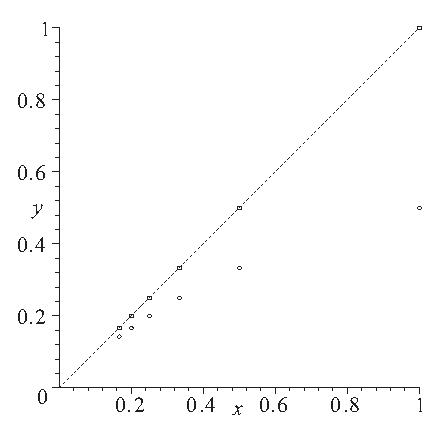
\includegraphics{figps-sec93-1.eps}
\end{center}
%
\item From the graph, we see that function $f$ is an injection.  We also see that the range of 
$f$ is the interval $\left[ 0, 1 \right)$, and hence, $f$ is a surjection.  

\item Since $f$ is a bijection, we conclude that $\left[0, 1 \right] \approx \left[ 0, 1 \right)$.
\end{enumerate}

\item Let $g: \left[ 0, 1 \right) \to \left( 0, 1 \right)$ by
\begin{equation} \notag
g \left( x \right) = 
\begin{cases}
\dfrac{1}{2}           &\text{if $x=0$} \\
%                      &                      \\
\dfrac{1}{n+1}         &\text{if $x=\dfrac{1}{n}$ for some $n \in \mathbb{N}$} \\
%                      &                      \\
x        &\text{otherwise}
\end{cases}
\end{equation}
%
\begin{enumerate}
\item The following graph shows some of the graph of the function $g$.  The points marked with a small square on the line $y = x$ indicate the points that have been removed from this line.  They have been replaced by the points marked with a small circle.  The graph shows 6 points that have been removed and the 6 points that have replaced them.  The process continues, but this is not shown on the graph.  Notice that the point $\left( 0, \dfrac{1}{2} \right)$ has been added, and there is no point on the graph with $x = 1$ since 1 is not in the domain of $g$.

\begin{center}
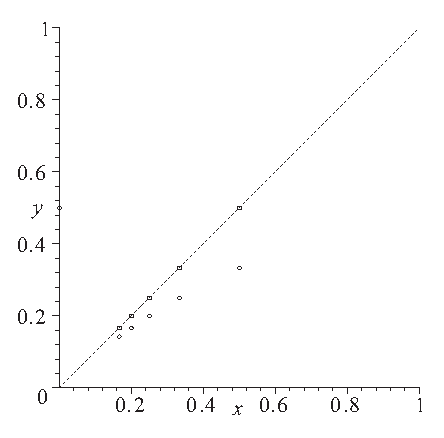
\includegraphics{figps-sec93-2.eps}
\end{center}
%
\item From the graph, we see that function $g$ is an injection.  We also see that the range of 
$g$ is the open interval $\left( 0, 1 \right)$, and hence, $g$ is a surjection.  

\item Since $g$ is a bijection, we conclude that $\left[0, 1 \right) \approx \left( 0, 1 \right)$.
\end{enumerate}

\item Part~(1) and Part~(2) show that the intervals $\left[0, 1 \right]$, $\left[0, 1 \right)$, and $\left(0, 1 \right)$ are all equivalent.  Therefore, each of the intervals is uncountable and has cardinality $\boldsymbol{c}$.


\end{enumerate}


\end{enumerate}

\hbreak
\endinput



\end{document}
